%!TEX encoding = UTF-8 Unicode
% $Id: onlisp-cn.tex 11 2011-06-09 06:09:31Z binghe $

%% On Lisp (Chinese Translation)
%% Translator: Chun Tian (binghe), Kov Chai, and others.
%% Compiling on TeXlive 2007

%\documentclass[fancyhdr]{ctexbookutf8}
\documentclass[a4paper,10pt,fleqn]{book}
\usepackage[hmargin={3cm,2cm}, vmargin={2.5cm,2cm}]{geometry}
\usepackage{graphics}
\usepackage{tikz}
\usetikzlibrary{arrows}
\usepackage{graphicx}
\usepackage{subfigure}
\graphicspath{{./figures/}}
\usepackage[pdfusetitle=false,
            pdftitle={On Lisp: Common Lisp 高级编程技术},
            hyperindex,
            bookmarksnumbered=true,
            bookmarksopen=true,
            breaklinks=true,
            colorlinks=true]{hyperref}
\usepackage{onlisp-cn}
\XeTeXlinebreaklocale "zh"
\XeTeXlinebreakskip = 0pt plus 1pt minus 0.1pt
\usepackage{makeidx}
\makeindex

\begin{document}
\pagestyle{empty}
%!TEX encoding = UTF-8 Unicode
% $Id: terms.tex 3 2009-08-07 06:58:03Z binghe $

%% 自定义符号
\newcommand{\onlisp}{\href{http://www.paulgraham.com/onlisp.html}{《\emph{On Lisp}》}}
\newcommand{\lexpr}{$\lambda$--表达式}
\newcommand{\sq}{\texttt{\#'}}
\newcommand{\bq}{反引用}
\newcommand{\comma}{逗号}
\newcommand{\commaat}{逗号--at}
\newcommand{\abbrev}{缩略语}

% intern & unintern appears on \ref{sec:avoiding_caption_with_gensyms}, chap 9
\newcommand{\gensym}{生成符号}
\newcommand{\intern}{约束}
\newcommand{\unintern}{未约束}


%% 内部词典 (多次出现或者不确定应如何翻译的词汇, 以便快速修改)
\newcommand{\utility}{实用工具} %% 1333 页, 英汉信息技术词典 (ISBN 7-111-09649-5)
\newcommand{\bup}{自底向上程序设计} %% 157 页, 同上
\newcommand{\cons}{点对}
\newcommand{\anaphoric}{首语重复}
\newcommand{\anaphor}{首语重复}

%% unknown
\newcommand{\inversion}{逆} %% 倒置物
\newcommand{\gv}{广义变量} %% generalized variable

\newcommand{\continuation}{续延}

%%% Local Variables:
%%% coding: utf-8
%%% mode: latex
%%% TeX-master: "onlisp-cn"
%%% End:


\frontmatter
%!TEX encoding = UTF-8 Unicode
% $Id: title.tex 3 2009-08-07 06:58:03Z binghe $

%% TITLE PAGE

\title{On Lisp}
\subtitle{Common Lisp 高级编程技术}
\author{Paul Graham}

\maketitle

\vfill
Copyright \copyright\ 2007 Paul Graham

原书站点: \href{http://www.paulgraham.com/onlisp.html}%
{\texttt{http://www.paulgraham.com/onlisp.html}}


\clearpage

~
\vfill
\begin{center}
  谨以此书献给我的家人和~Jackie。
\end{center}
\vfill

\newpage

~
\vfill
\begin{center}
  $\lambda$
\end{center}
\vfill

%%% Local Variables:
%%% coding: utf-8
%%% mode: latex
%%% TeX-master: "onlisp-cn"
%%% End:


\pagenumbering{roman}
%!TEX encoding = UTF-8 Unicode
% $Id: 00-preface-cn.tex 3 2009-08-07 06:58:03Z binghe $

\chapter*{译者序}
\label{chap:preface-cn}

《On Lisp》不是一本~Lisp 的入门教材,它更适合读过%
\href{http://www.paulgraham.com/acl.html}{《ANSI Common Lisp》}%
或者\href{http://gigamonkeys.com/book/}{《Practical Common Lisp》}%
的~Lisp 学习者。它对~Lisp 宏本身及其使用做了非常全面的说明,同时自底向
上的编程思想贯穿全书,这也是本书得名的原因,即,基于~Lisp,扩展~Lisp。

原作者~\href{http://www.paulgraham.com/}{Paul Graham} 同时也
是《ANSI Common Lisp》一书的作者。

《On Lisp》成书早在~1994 年~ANSI Common Lisp 标准发布以前,书中使用了许多古
老的~Lisp 操作符,其中一些代码已经无法在最新的~Common Lisp 平台上执行了。
所以译文里所有的源代码都被改成了符合现行~Common Lisp 标准的形式,凡译者
修改过的地方都会以脚注的形式注明。

我要特别感谢来自~AMD/ATI 的~Kov Chai\footnote{
\href{mailto:tchaikov@gmail.com}{\texttt{tchaikov@gmail.com}}}
同学,他独立翻译了第~\ref{chap:returning_functions},
\ref{chap:functions_as_representation},
\ref{chap:nondeterminism},
\ref{chap:parsing_with_atns},
\ref{chap:object-oriented_lisp} 章及附录,并对全书进行了细致的校对。
另外~Kov Chai 还主导了本书的~\LaTeX~排版工作。

感谢~Yufei Chen\footnote{
\href{mailto:cyfdecyf@gmail.com}{\texttt{cyfdecyf@gmail.com}}}
同学提供改进排版的补丁。他还参与了第~\ref{chap:multiple_processes}
章的翻译工作。

Mathematical Systems, Inc. 的~Lisp 程序员~Jianshi Huang\footnote{
\href{mailto:jianshi.huang@gmail.com}{\texttt{jianshi.huang@gmail.com}}}
同学是我最初翻译本书时的合作者,他翻译了第~\ref{chap:prolog} 章,并
初步校对了本书前三章。

\vfill
\hfill \emph{Chun TIAN (binghe)}\footnote{
  \href{mailto:binghe.lisp@gmail.com}{\texttt{binghe.lisp@gmail.com}}}

\hfill \emph{NetEase.com, Inc.}
\vfill


%%% Local Variables:
%%% coding: utf-8
%%% mode: latex
%%% TeX-master: "onlisp-cn"
%%% End:

\renewcommand{\chaptermark}[1]{%
              \markboth{#1}{}}%
\renewcommand{\sectionmark}[1]{\markright{#1}}%
\pagestyle{preface}
%!TEX encoding = UTF-8 Unicode
% $Id: 0-preface.tex 5 2009-08-07 08:40:43Z binghe $

\chapter*{前言}
\label{chap:preface}

本书适用于那些想更上一层楼的~Lisp 程序员。书中假设读者已经初步了解~Lisp,但不要求有丰富的
编程经验。最初几章里会重温很多基础知识。我希望这些章节也会让有经验的~Lisp 程序员感兴趣,
因为它们以崭新的视角展示了熟知的主题。

通常很难一语道清一门编程语言的精髓,但~John
Foderato\index{Foderaro, John K.}\note{v} 的话已经很贴切了:

\begin{quote}
  Lisp 是一门可编程的编程语言。
  (Lisp is a programmable programming language.)
\end{quote}

这难免以偏概全,但这种让~Lisp 随心而变的能力,在很大程度上正是~Lisp 专
家和新手的不同之处。在自上而下,把程序逐渐具体化,用编程语言实现设计的
同时,资深的~Lisp 程序员也实践着自底向上的方法,他们通过创建语言来描
述程序的行为。本书教授自底向上编写程序的方法,因为这是~Lisp 与
生俱来的强项。

\section*{自底向上的设计~(Bottom-up Design)}
\label{sec:bottom-up_design}
\index{bottom-up design 自底向上的设计}

随着软件复杂度的增长,自底向上设计的重要性也日益提高。今天的程序可能不得不面对极其复杂
甚至开放式的需求。在这种情况下,传统的自上而下方法有时会失效。一种新的编程风格应运而生,
它和当前大部分计算机科学课程的思路截然不同:
一个自底向上的程序由一系列的层写成,每一层都作为更高一层的编程语言。
X Window\index{X Window} 和~\TeX\index{TeX@\TeX} 就是这种程序设计风格的典范。

本书有两层主题: 首先,对以自底向上的方法编制的程序来说,Lisp 语言是不二之选,
反过来,编写~Lisp 程序的话,采用自底向上的编程风格也是理所当然的。因此《On Lisp》将吸引两类读者。
对于那些有兴趣编写可扩展程序的人,本书将告诉你如果有了合适的语言,你能做些什么。对于~Lisp
程序员来说,本书提供了第一手的实践指南,指引他们把~Lisp 的优势发挥到极致。

本书选用现在的这个书名是为了强调自底向上编程对于~Lisp 的重要性。你不再仅仅是用
~Lisp 编写程序,\emph{在~Lisp 之上~(On Lisp)},你可以构造自己的语言,然后再用
这个语言来写程序。

尽管用任何语言都可以写出自底向上风格的程序,但~Lisp 对于这种编程风格来
说是最自然的载体。在~Lisp 里,自底向上的设计并不是那种仅为少见的大型程
序或者高难程序服务的专门技术。任何规模的程序都可以在一定程度上以这种方
式编写。Lisp 从一开始就被设计成可扩展的语言。这种语言本身基本上就是一
个~Lisp 函数的集合,这些函数和你自己定义的没有本质区别。更进一步,Lisp
函数可以表达成列表,而列表同时也是~Lisp 的数据结构。这就意味着你可以写
出能生成~Lisp 代码的~Lisp 函数。

一个好的~Lisp 程序员必须懂得如何利用上述这种可能性。通常的途径是定义
一种称为\emph{宏}的操作符。驾驭宏是从编写正确的~Lisp 程序走向编写漂亮
的程序过程中最重要的一步。入门级~Lisp 书籍给宏留下的篇幅仅限于一个宏的简
短的概述: 解释一下宏是什么,加上几个例子蜻蜓点水地提一下,说能用它实
现一些奇妙的东西。不过本书会给予这些奇妙的东西特别的重视。这里的
目标之一就是把所有关于宏的知识作一次总结,在以往,人们只能从使用宏的
经验和教训中来吸取这些知识。

一般来说,Lisp 的入门读物都不会强调~Lisp 和其他语言的区别,这情有可原。
它们必须想办法把知识传授给那些被教育成只会用~Pascal 术语来构思程序的
学生。如果非要细究这些区别的话,只会把问题复杂化: 例如~\texttt{defun}
虽然\emph{看起来}像一个过程定义,但实际上,它是一个编写程序的程序,这个程
序生成了一段代码,而这段代码新建了一个函数对象,然后用函数定义时给出的
第一个参数作为这个函数对象的索引。

本书的目的之一就是解释究竟是什么使~Lisp 不同于其他语言。刚落笔时,
我心里明白,同等条件下自己会更倾向于用~Lisp 而不
是~C、Pascal 或~Fortran 来写程序。我也知道这不只是个人好恶的问题。但当
意识到就要郑重其事地告诉大家~Lisp 语言在某些方面更优秀时,我发
现应该做好准备,说说到底为什么。

曾有人问~Louis Armstrong\index{Armstrong,Louis} 什么是爵士乐\index{jazz 爵士乐},
他答道~``如果你问爵士乐是什么,那你永远不会知道。''
但他确实以一种方式回答了这个问题:他向世人\emph{展示}了什么是爵士乐。同样也只有一种方式
来解释~Lisp 的威力\index{programming languages 编程语言!expressive power of 的表达能力},就是演示那些对于其他语言来说极其困难甚至不可能实现的技术。多数关于编
程的书籍,包括~Lisp 编程书籍,采用的都是那些你可以用任何其它语言编写的程序。
《On Lisp》 涉及的多是那些只能用~Lisp 写的程序。可扩展性,\bup,
交互式开发,源代码转换,嵌入式语言\pozhehao{}这些都是~Lisp 展示其高级特性的舞台。

当然从理论上讲,任意图灵等价的编程语言能做的事,其它任何语言都可以做
到。但这种能力和编程语言的能力却完全是两码事。理论上,任何你能用编程语言
做到的事,也可以用图灵机\index{Turing Machines 图灵机}来做,但实际上在图
灵机上编程得不偿失。

所以,当我说这本书是关于如何做那些其他语言力所不及的事情的时候,我并非指数学意义上的~
``不可能'',而是从编程语言的角度出发的。这就是说,如果你不得不用~C 来写本书中的一些程序,
你可能需要先用~C 写一个~Lisp 编译器。举个例子,在~C 语言里嵌入~Prolog\pozhehao{}你能想象
这需要多少工作量吗?
第~\ref{chap:prolog} 章将说明如何用~180 行~Lisp 做到这一点。

尽管我希望能比单单演示~Lisp 的强大之处做得更多。我也想解释\emph{为何}~Lisp 与众不同。
这是一个更微妙的问题,这个问题是那么难回答,它无法使用诸如~``符号计算'' 这样的术语来搪塞。
我将尽我所学,尽可能清楚明白地解释这些问题。

\section*{本书规划}
\label{sec:plan_of_the_book}

由于函数是~Lisp 程序的基础,所以本书开始的几章是有关函数的。
第~\ref{chap:functions} 章解释~Lisp 函数究竟是什么,以及它们带来了何种可能。
第~\ref{chap:functional_programming} 章讨论函数型编程的优点,这是~Lisp 程序最主要的
风格。
第~\ref{chap:utility_functions} 章展示如何用函数来扩展~Lisp。
第~\ref{chap:returning_functions} 章建议了一种新的抽象方式,即返回其他函数的函数。
最后,第~\ref{chap:functions_as_representation} 章显示了怎样使用函数来取代传统的数据
结构。

本书剩下的篇幅则更加关注宏。一部分原因是因为宏本身的内容就更多些,
一部分是因为至今尚无著作完整地介绍过宏的方方面面。
第~\ref{chap:macros}--\ref{chap:other_macro_pitfalls} 章构成了一套关于宏技术的完整教程。
学完这个教程后,你将了解一个有经验的~Lisp 程序员所知的关于宏的大多数内容: 它们如何工作;怎样定义,
测试,以及调试它们;
何时应该使用以及何时不应该使用宏;宏的主要类型;怎样写生成宏展开代码的程序;
宏风格一般如何区别于~Lisp 风格;
以及怎样甄别和改正每一种宏特有的问题。

在这套宏教程之后,第~\ref{chap:classic_macros}--\ref{chap:destructuring}
章展示了一些可以用宏来构造的强有力的抽象机制。
第~\ref{chap:classic_macros} 章展示如何写典型的宏\pozhehao{}那些创造上下文,
或者实现循环或条件判断的宏。
第~\ref{chap:generalized_variables} 章解释宏在操作普通变量中的角色。
第~\ref{chap:computation_at_compile-time}
章展示宏如何通过将计算转移到编译期来使程序运行得更快。第~\ref{chap:anaphoric_macros}
章介绍了指代~(anaphoric) 宏,它允许你在程序里使用代词。
第~\ref{chap:macro_returning_functions}
章展示了宏如何为第~\ref{chap:returning_functions} 
章里定义的函数生成器提供一个更便利的接口。第~\ref{chap:macro-defining_macros}
章展示了如何使用定义宏的宏来让~Lisp 为你写程序。
第~\ref{chap:read-macros} 章讨论读取宏~(read-macro),
以及第~\ref{chap:destructuring} 章,解构宏。

第~\ref{chap:a_query_compiler} 章开始了本书的第四部分,这一部分的重点是嵌入式语言。
第~\ref{chap:a_query_compiler} 章通过展示同一个程序,一个回答数据库查询的程序,
先是用解释器,然后用真正的嵌入式语言,来介绍这一主题。
第~\ref{chap:continuations} 章展示了如何将续延~(continuation) 的概念引入~Common Lisp
程序,这是一种描述延续性计算的对象。续延是一个强有力的工具,
可以用来实现多进程和非确定性选择。至于如何把这些控制结构嵌入到~Lisp 中,
第~\ref{chap:multiple_processes} 和
~\ref{chap:nondeterminism} 章将对此进一步展开讨论。
非确定性听上去好像是一种具有非同寻常能力的抽象机制,它让你的程序似乎能未卜先知。
第~\ref{chap:parsing_with_atns} 和~\ref{chap:prolog} 章展示了两种嵌入式语言,
它们证明了非确定性绝非浪得虚名: 一个完整的~ATN 解析器,以及一个嵌入式~Prolog,总共才~200
行代码\note{viii}。

这些程序的长短本身并没有什么意义。如果你喜欢写像天书一样的程序,没人知道
你用~200 行代码能写出什么。
关键在于,这些程序并非靠编程技巧才变得短小\index{brevity 简洁},而是由于它们
是以~Lisp 所固有的,自然的方式写成的。
第~\ref{chap:parsing_with_atns} 和~\ref{chap:prolog} 章的用意并不是教授如何用一页
代码实现~ATN 解析器或者用两页实现~Prolog,
而是想说明这些程序,当给出它们最自然的~Lisp 实现的时候是如此的简洁。后面这两个章节的嵌入式
语言用实例证明了我开始时的两个观点:
Lisp 对于以自底向上的编程风格来说是一种自然的语言,同时自底向上的编程风格也是编写~Lisp
程序理所当然的方式。

本书以关于面向对象编程的讨论做结,其中特别讨论了~\textsc{clos},Common Lisp 对象系统。
把这一主题留到最后,
我们可以更加清楚地看到,面向对象的编程方式是一种扩展,这种扩展植根于一些早已存在于~Lisp
的思想之上。它是多种可以建立\emph{在~Lisp 上}的抽象之一。

自成一章的附注始于第~\pageref{chap:notes} 页。这些注释里包括参考文献,补充或者替换的
代码,
或者是有关~Lisp,但和当前主题没有直接联系的一些文字。注释是用页面留白上的小圆圈标注出来的,就像这样
\bubblenote。另外还有一个关于包~(package) 的附录,在第~\pageref{chap:packages} 页。

去纽约逛一圈或许对世界上的多数文化会有走马观花的了解,同样,在把~Lisp 作为一门可扩展编程语言来学习
也能接触到大部分的~Lisp 技术。这里描述的大多数技术通常都已为~Lisp 社区所熟知,
但很多内容至今也没有在任何地方有记载。而有些问题,例如宏的作用或变量捕捉的本质,
甚至对于许多很有经验的~Lisp 程序员来说也只是一知半解。

\section*{示例}
\label{sec:examples}

Lisp 是个语言家族。由于~Common Lisp 仍然是广泛使用的方言,本书的大部
分示例都是使用~Common Lisp 编写的。在~1984 年,Guy Steele\index{Steele, Guy Lewis Jr.} 
的~\emph{Common Lisp: the Language}%
\index{Common Lisp: the Language@\emph{Common Lisp: the Language}}
(\textsc{cltl}1\index{CLTL@\textsc{cltl}|see{\emph{Common Lisp: the Language}}}) 首
次定义了这门语言\index{Common Lisp!definition of 的定义}。1990 年,该书
第二版~(\textsc{cltl}2) \note{ix} 出版以后,这一定义被取而代之,
\textsc{cltl}2 可能会让位于将来的~\textsc{ansi} 标准\index{ANSI Common
  Lisp@\textsc{Ansi} Common Lisp}。

本书包含数百个示例,小到简单的表达式,大至可运行的~Prolog 实现。书中代码的编写,
尽量照顾到了各个细节,使得它们可以在任何版本的~Common Lisp 上运行。
有极少数例子需要用到~\textsc{cltl}1 规范之外的特性,这些示例将会在正文中加以明确的标识。
最后几个章节里包括了一些~Scheme 的示例代码,这些代码也会有清楚的标记。

所有代码可以通过匿名~\textsc{FTP} 从~\texttt{endor.harvard.edu} 下载,
在~\texttt{pub/onlisp} 目录里。问题和评论可以发到~\texttt{onlisp@das.harvard.edu}。

\section*{致谢}
\label{sec:acknowledgements}

写此书时,我要特别感谢~Robert Morris 的帮助。我经常去向他寻求建议,每次都会满载而归。
本书的一些示例代码就来自他,包
括~\pageref{fig:avoiding_capture_with_closure}
页上的一个~\texttt{for} 版本,
\pageref{fig:anaphoric_variants_of_common_lisp_operators} 页上
的~\verb|aand| 版本,\pageref{fig:matching_function} 页
的~\texttt{match},\pageref{fig:correct_choose_in_scheme} 页的广度优
先~\texttt{true-choose},以及第~\ref{sec:prolog:an_interpreter} 节
的~Prolog 解释器。事实上,整本书都反映~(有时基本是抄录) 了过去七年来我
跟~Robert 之间的对话。(谢谢你,rtm!)

我还要特别感谢~David Moon,他仔细阅读了大部分手稿并且给出许多非常有用的评论。
第~\ref{chap:generalized_variables}
章是按照他的建议完全重写了的,\pageref{example:capture} 页关于变量捕捉
的示例代码也是他提供的。

我很幸运地拥有~David Touretzky 和~Skoma Brittain 两位技术审稿人。有些章节就
是在他们的建议下追加或者重写的。
第~\pageref{func:true-choice} 页给出的另一个非确定性选择操作符就出自~David Toureztky 的一个建议。

还有一些人欣然阅读了部分或全部手稿,他们是~Tom Cheatham,Richard Draves
(他在~1985 年也帮助重写了~\texttt{alambda} 和~\texttt{propmacro}),
John Foderaro,David Hendler,George Luger,Robert Muller,Mark
Nitzberg\index{Nitzberg, Mark|see {joke, pratical}}\index{joke, pratical|see {Nitzberg, Mark}},以及~Guy Steele。 

我感谢~Cheatham 教授以及整个哈佛,他们为我提供了撰写此书的条件。也感谢~Aiken
实验室的全体成员,包括~Tony Hartman,Janusz Juda,Harry Bochner,以及~Joanne
Klys。

Prentice Hall 的工作人员干得非常出色。我为与~Alan Apt 这位优秀的编辑和好伙伴一
起共事感到幸运。同时也感谢~Mona Pompili,Shirley Michaels,以及~Shirley
McGuire 的组织工作和他们的幽默。

剑桥~Bow and Arrow 出版社的无与伦比的~Gino Lee 制作了封面。封面上的那棵树暗示了第~\pageref{sec:functions_from_lists} 页上
的观点。

本书使用~\LaTeX{} 排版,这是一种由~Leslie Lamport 在~Donald Knuth 的~\TeX{}
基础上设计的语言,
另外使用了来自~L. A. Carr,Van Jacobson 和~Guy Steele 的宏。插图由~John
Vlissides 和~Scott Stanton 设计的~idraw 完成。
整本书用~L. Peter Deutsch 的~Ghostscript 生成之后,在~Tim Theisen
的~Ghostview 里预览。Chiron Inc. 公司的~Gary Bisbee 制作了能用来进行照相制版的拷贝。

我要感谢其他许多人,包括~Paul Becker,Phil Chapnick,Alice Hartley,
Glenn Holloway,Meichun Hsu,Krzysztof Lenk,Arman Maghbouleh,Howard
Mullings,Nancy Parmet,Robert Penny,Gary Sabot,Patrick Slaney,Steve
Strassman,Dave Watkins,Weickers\index{Weicker,Jacqueline J.} 一家,
还有~Bill Woods。

最后,我要感谢我的父母,谢谢他们为我树立的榜样还有对我的鼓励;还有~Jackie,要是我听得进他说的话,
或许能学到点什么。

\vspace{5ex}

我希望阅读此书是件乐事。在所有我知道的语言中,Lisp 是我的最爱,只因它是最优美
的。本书着眼于最~Lisp 化的~Lisp。写作这本书的过程充满了乐趣\index{fun 乐趣},
愿你在阅读此书时能感同身受。

\vspace{1in}

\hfill\emph{Paul Graham}

\vfill

%%% Local Variables:
%%% coding: utf-8
%%% mode: latex
%%% TeX-master: "onlisp-cn"
%%% End:

\tableofcontents
\mainmatter
\pagestyle{main}
\renewcommand{\chaptermark}[1]{%
              \markboth{\CJKprechaptername~\thechapter~\CJKchaptername\quad#1}{}}
\renewcommand{\sectionmark}[1]{\markright{#1}}
%!TEX encoding = UTF-8 Unicode
% $Id: 1-the_extensible_language.tex 17 2014-03-09 13:05:41Z binghe $

\chapter{可扩展语言}
\label{chap:the_extensible_language}

不久前,如果你问~Lisp 是用来干什么的,很多人会回答说~``人工智能\index{artificial
  intelligence 人工智能}~(artificial intelligence)''。事实上,Lisp 和人工智能之间的联系只是历史的偶然。Lisp 由
~John McCarthy\index{McCarthy, John} 发明,同样是他首次提出了~``人工智能'' 这一名词。
那时他的学生和同事用~Lisp 写程序,于是它就被称作一种~\textsc{AI} 语言。这个典故在
~1980 年代~\textsc{AI} 短暂升温时又被多次提起,到现在已经差不多成了习惯。

幸运的是,``\textsc{AI} 并非~Lisp 的全部''的观点已经开始为人们所了解。近年来软硬件
的长足发展已经让~Lisp 走出了象牙塔:
它目前用于~GNU Emacs\index{GNU Emacs}\index{Emacs|see{GNU Emacs}},Unix 下最好的文本编辑器;AutoCAD\index{AutoCAD},
工业标准的桌面~\textsc{CAD} 程序;还有~Interleaf\index{Interleaf},
领先的高端出版系统。Lisp 在这些程序里的应用跟~\textsc{AI} 已经没有了任何关系。

如果~Lisp 不是一种~\textsc{AI} 语言,那它是什么?与其根据那些使用它的公司来判断~Lisp,
我们不如直接看看语言本身。有什么是你可以用~Lisp 做到,而其他语言没法做到的呢?
Lisp 的一个最显著的优点是可以对其量身定制,让它与用它写的程序相配合。Lisp 本身就是一个
~Lisp 程序,Lisp 程序可以表达成列表,
那也是~Lisp 的数据结构。总之,这两个原则意味着任何用户都可以为~Lisp 增加新的操作符,
而这些新成员和那些内置的操作符是没有区别的。

\section{渐进式设计}
\label{sec:design_by_evolution}
\index{evolution!design by}
\index{exploratory programming 探索式的编程}

由于~Lisp 赋予了你自定义操作符的自由,因而你得以随心所欲地将它塑造成你所需要的语言。\index{Lisp!defining features of}如果
你在写一个文本编辑器,那么可以把~Lisp 转换成专门写文本编辑器的语言。
如果你在编写~\textsc{CAD} 程序,那么可以把~Lisp 转换成专用于写~\textsc{CAD} 程序的语言。
并且如果你还不太清楚你要写哪种程序,那么用~Lisp 来写会比较安全。因为无论你想写哪种程序,
在你写的时候,Lisp 都可以演变成用于写\emph{那}种程序的语言。

你还没想好要写哪种程序?一样可以。对有些人来说,这种说法有点不对劲。
这和某种行事方式很不一样,这种方式有两步:(1) 仔细计划你打算做的事情,接下来~(2)
去执行它。按照这个逻辑,如果~Lisp 鼓励你在决定程序应该如何工作之前就开始写程序,
它只不过是怂恿你匆忙上马,草率决定而已。

事实并非如此。先计划再实施的方法可能是建造水坝或者发起战役的方式,但经验并未表明
这种方法也适用于写程序。
为什么?也许是因为计算机的要求太苛刻了。也许是因为程序中的变数比水坝或者战役更多。
或许老方法不再奏效的原因,是因为旧式的冗余观念不适用于软件开发:如果一座大坝浇铸了额外的~$30\%$
的混凝土,那是为以后的误操作留下的裕量,但如果一个程序多做了额外~$30\%$ 的工作,
那\emph{就是}一个错误。

很难说清原来的办法为什么会失效,但所有人都心知肚明老办法不再行之有效。究竟有几次软件按时
交付过?有经验的程序员知道无论你多小心地计划一个程序,当你着手写它的时候,之前制定的计划在
某些地方就会变得不够完美。
有时计划甚至会错得无可救药。却很少有~``先策划再实施'' 这一方法的受害者站出来质疑它的有效性。
相反,他们把这都归咎于人为过失:
只要计划做的更周详,所有的问题就都可以避免。就算是最杰出的程序员,在进行具体实现的
时候也难免陷入麻烦,因此要人们必须具备\emph{那种}程度的前瞻性可能过于苛求了。
也许这种先策划再实施的方法可以用另外一种更适合我们自身限制的方法取而代之。

如果有合适的工具,我们完全可以换一种角度看待编程。为什么我们要在具体实现之前计
划好一切呢?盲目启动一个项目的最大危险是我们可能不小心就使自己陷入困境。但如果
存在一种更加灵活的语言,是否能为我们分忧呢?我们可以,而且确实如此。
Lisp 的灵活性带来了全新的编程方式。在~Lisp 中,可以边写程序边做计划
\index{planning 计划}。

为什么要等事后诸葛亮呢?正如~Montaigne\index{Montaigne@{de Montaigne Michel}}\footnote{译者注:
Montaigne,即~Michel Ryquem de Montaigne。国内一般译作~``蒙田''。他是
法国文艺复兴后期重要的人文主义学者,他曾说过~``我本人就是作品的内容''。}
所发现的那样,
如果要理清自己的思路,试着把它写下来会是最好的办法。一旦你能把自己从陷入困境的危险中
解脱出来,那你就可以完全驾驭这种可能性。边设计边施工有两个重要的后果:
程序可以花更少的时间去写,因为当你把计划和实际动手写放在一起的时候,你总可以把精力集中在一个
实际的程序上;然后让它变得\emph{日益完善},因为最终的设计必定是进化的成果。
只要在把握你程序的命运时坚持一个原则:
一旦定位错误的地方,就立即重写它,
那么最终的产品将会比事先你花几个星期的时间精心设计的结果更加优雅。

Lisp 的适应能力使这种编程思想成为可能。确实,Lisp 的最大危险是它可能会把你宠坏了。
使用~Lisp 一段时间后,你会开始对语言和应用程序之间的结合变得敏感,
当你回过头去使用另一种语言时,总会有这样的感觉:它无法提供你所需要的灵活性。

\section{\bup}
\label{sec:programming_bottom-up}

有一条编程原则由来已久:作为程序的功能性单元不宜过于臃肿。如果程序里某些组件的规模增长超过了它可读的程度,它就会成为一团乱麻,藏匿其中的错误就好像巨型城市里的逃犯那样难以捉摸。这样的软件将难以阅读,难以测试,调试起来也会痛苦不堪。

按照这个原则,大型程序必须细分成小块,并且程序的规模越大就应该分得越细。
但你怎样划分一个程序呢?
传统的观点被称为\emph{自顶向下的设计}\index{top-down design 自顶向下的设计}:
你说~``这个程序的目的是完成这七件事,那么我就把它分成七个主要的子例程。
第一个子例程要做这四件事,所以它将进一步细分成它自己的四个子例程'',如此这般。
这一过程持续到整个程序被细分到合适的粒度\pozhehao{}每一部分都足够大可以做一些实际的事情,
但也足够小到可以作为一个基本单元来理解。

有经验的~Lisp 程序员用另一种不同的方式来细化他们的程序。和自顶向下的设计方法类似,
他们遵循一种叫做\emph{自底向上的设计}\index{bottom-up design 自底向上的设计}
原则\pozhehao{}即通过改变语言来适应程序。在~Lisp 中,你不仅是根据语言向下编写程序,
也可以根据程序向上构造语言。在编程的时候你可能会想
~``Lisp 要是有这样或者那样的操作符就好了。''
那你就可以直接去实现它。之后,你会意识到使用新的操作符也可以简化程序中另一部分的设计,如此种种。
语言和程序一同演进。
就像交战两国的边界一样,语言和程序的界限不断地移动,直到最终沿着山脉和河流确定下来,
这也就是你要解决的问题本身的自然边界。最后你的程序看起来就好像语言就是为解决它而设计的。
并且当语言和程序彼此都配合得非常完美时,你得到的将是清晰、简短和高效的代码。

需要强调的是,自底向上的设计并不意味着只是换个次序写程序。当以自底向上的方式工作时,
你通常写出来的程序会彻底改观。你将得到一个带有更多抽象操作符的更大的语言,
和一个用它写的更精练的程序,
而不是单个的整块的程序。你得到将是拱\index{arch 拱!bottom-up program as 自底向上
编程作为}而非梁\index{bottom-up design 自底向上的设计!and shape of programs}。

在典型的程序中,一旦把那些仅仅是做非逻辑工作的部分抽象掉,剩下的代码就短小多了;
你构造的语言越高阶,程序从上层逻辑到下层语言的距离就越近。这有几个好处:
\begin{enumerate}
\item
  通过让语言担当更多的工作,自底向上设计产生的程序会更加短小轻快。一个更短小的程序就不必
  划分成那么多的组件了,
  并且更少的组件意味着程序会更易于阅读和修改。更少的组件也使得着组件之间的连接会更少,
  因而错误发生的机会也会相应减少。
  一个机械设计师往往努力去减少机器上运动部件\index{moving parts 运动部件}的数量,
  同样有经验的~Lisp 程序员使用自底向上的设计方法来减小他们程序的规模和复杂度。
\item
  自底向上的设计促进了代码重用\index{re-use of software 代码重用}。当你
  写两个或更多程序时,许多你为第一个程序写的工具也会对之后的程序开发有
  帮助。一旦积累下了雄厚的工具基础,写一个新程序所耗费的精力和从原
  始~(raw) Lisp 环境白手起家相比,前者可能只是后者的几分之一。
\item
  自底向上的设计提高了程序的可读性。一个这种类型的抽象要求读者理解一个通用操作符,
  而一个具体的函数抽象要求读者去理解的则是一个专用的子例程。\footnote{~``但是没人能读懂你的
    程序,除非理解了所有新的实用函数''。要想知道为什么这种认识是一种误解,
    请参考第~\ref{sec:density} 节。}
\item
  由于自底向上的设计驱使你总是去关注代码中的模式,这种工作方式有助于理清设计程序时的思路。
  如果一个程序中两个关系很远的组件在形式上很相似,你就会因此注意到这种相似性,然后也许会以
  更简单的方式重新设计程序。
\end{enumerate}
% from 88:CrazyCube and others,2007-12-07
对于其他非~Lisp 的语言来说,自底向上的设计在某种程度上也是可能的。
大家熟悉的库函数就是自底向上设计的一种体现。
然而在这方面,Lisp 还能提供比其他语言更强大的威力,而且在以~Lisp 风格编程时,
扩展这门语言的重要性也相应提高了,
所以~Lisp 不仅是一门不同的编程语言,而且是一种完全不一样的编程方式。

确实,这种开发风格更适合那种可以小规模开发的程序。不过,与此同
时,它却让一个小组所能做更多的事情。在《人月神话》\index{Mythical
  Man--Month, The@\emph{Mythical Man--Month, The} 人月神话}一书
中,Frederick Brooks\index{Brooks, Frederik P.} 提出~``一组程序员的生产力并不随人员的数量
呈线性增长''。\note{5}
随着组内人数的增加,个体程序员的生产力\index{productivity 生产力}将有所下降。Lisp
编程经验以一种更加令人振奋的方式重申这个定律:随着组内人数的减少,个体
程序员的生产力将会提高。一个小组取得成功的原因,仅仅是因为它的规模相对较小。
如果一个小组能利用~Lisp 带来的技术优势,它必定会走向成功。

\section{可扩展软件}
\label{sec:extensible_software}

随着软件复杂度的提高,编程的~Lisp 风格也变得愈加重要。专业用户现在对软件的要求如此之多以致
于我们几乎无法预见到他们的所有需求。就算用户自己也没办法预测到他们所有的需求。但如果我们不
能给他们一个现成的软件,让它能完成用户想要的每个功能,那么我们也可以交付一个可扩展的软件。
我们把自己的软件从单单一个程序变成了一门编程语言,然后高级用户就可以在此基础上构造他们需要
的额外特性。

自底向上的设计很自然地产生了可扩展的程序。最简单的自底向上程序包括两层:语言和程序。复杂
的程序可以被写成多个层次,每一层作为其上层的编程语言。如果这一哲学被一直沿用到最上面的那层,
那最上面的这一层对于用户来说就变成了一门编程语言。
这样一个可扩展性\index{extensibility 可扩展性}体现在每一层次的程序,与那些先按照传统
黑盒方法写成,事后才加上可扩展性的那些系统相比,更有可能成为一门好得多的编程语言。

X--Window\index{X Window} 和~\TeX{}\index{TeX@\TeX} 就是遵循这一设计原则编写而成的
早期典范。在~1980 年代,更强大的硬件使得新一代的程序能使用~Lisp 
作为它们的扩展语言。首先是~GNU Emacs\index{GNU Emacs},流行的~Unix 文本编辑器。
紧接着是~AutoCAD\index{AutoCAD},
第一个把~Lisp 作为扩展语言的大型商业软件。1991 年~Interleaf\index{Interleaf} 发布了他们软件的新版本
,它不仅采用~Lisp 作为扩展语言,甚至该软件大部分就是用~Lisp 实现的。

Lisp 这门语言特别适合编写可扩展程序,主要原因是因为它本身就是一个可扩展的程序。
如果你用~Lisp 写你的程序以便将这种可扩展性转移到用户那里,你事实上已经毫不费力地得到了一个
可扩展语言\index{programming languages 编程语言!extensible 可扩展的}。并且用~Lisp
扩展~Lisp 程序,和用一个传统语言做同样的事情相比,
它们的区别就好比面对面交谈和使用书信联系的区别。
如果一个程序只是简单提供了一些供外部程序访问的方式,以期获得可扩展性,那么我们最乐观的估计也无非是两个
黑箱之间彼此通过预先定义好的渠道进行通信。在~Lisp 里,这些扩展有权限直接访问整个底层程序。
这并不是说你必须授予用户你程序中每一个部分的访问权限\pozhehao{}只是说你现在有\emph{机会}决定
是否赋给他们这样的权限。\index{open systems 开放式系统}

当权限的取舍和交互式环境结合在一起,你就拥有了处于最佳状态的可扩展
性。任何软件,如果你想以它为基础,在其上进行扩展,为己所用,在你心中就好比有
了一张非常大,可能过于巨大的完整的蓝图。要是其中的有些东西不敢确定,该怎么
办?如果原始程序是用~Lisp 开发的,那就可以交互式地试探它:你可以检查它的
数据结构;你可以调用它的函数;你甚至可能去看它最初的源代码。这种反
馈信息让你能信心百倍地写程序\pozhehao{}去写更加雄心勃勃的扩展,并且会写得
更快。一般而言,交互式环境可以让编程更轻松,但它对写扩展的人来说尤其有用。

可扩展的程序是一柄双刃剑,但近来的经验表明,和钝剑相比,用户更喜欢双刃剑。可扩展的程序
看起来正在流行,无论它们是否暗藏危机。

\section{扩展~Lisp}
\label{sec:extending_lisp}

有两种方式可以为~Lisp 增加新的操作符:函数和宏。在~Lisp 里,你定义的函数和那些内置函数具有
相同的地位。如果想要一个新的改版的~\verb|mapcar|,那你就可以先自己定义,然后就像使用
~\texttt{mapcar} 那样来使用它。
例如,如果有一个函数,你想把从~1 到~10 之间的所有整数分别传给它,然后把函数的返回值组成的
列表留下,你可以创建一个新列表然后把它传给~\texttt{mapcar}:
\begin{lstlisting}
(mapcar fn
        (do* ((x 1 (1+ x))
              (result (list x) (push x result)))
            ((= x 10) (nreverse result))))
\end{lstlisting}
但这样做既不美观又没效率。\footnote{你也可以使用~Common Lisp 的~series 宏把代码
写得更简洁,但那也只能证明同样的观点,因为这些宏就是~Lisp 本身的扩展。}
换种办法,你也可以
定义一个新的映射函数~\texttt{map1-n} (见~\pageref{fig:mapping_functions} 页),
然后像下面那样调用它:
\begin{lstlisting}
(map1-n fn 10)
\end{lstlisting}
定义函数相对而言比较直截了当。而用宏来定义新操作符,虽然更通用,但不太容易理解。
宏是用来写程序的程序。这句话意味深长,深入地探究这个问题正是本书的主要目的之一。

深思熟虑地使用宏,可以让程序惊人的清晰简洁。这些好处绝非唾手可得。尽管到最后,宏将被
视为世上最自然的东西,但最初理解它的时候却会举步维艰。部分原因是因为宏比函数更加一般化,
所以编写的时候要考虑的事情更多。
但宏难于理解,最主要的原因是它\emph{太另类了}。
没有任何一门语言有像~Lisp 宏那样的东西。
所以学习宏,可能先要从头脑中清除从其他语言那里潜移默化接受的先入为主的观念。
这些观念中,首当其冲就是为那些陈词滥调所累的程序。
凭什么数据结构可以变化,并且其中的数据可以修改,而程序却不能呢?
在~Lisp 里,程序\emph{就是}数据,但其中深意需要假以时日才能体会到。

如果你需要花些时间才能习惯宏,那么这些时间绝对是值得的。即使像迭代这样平淡无奇的用法中,
宏也可以使程序明显变得更短小精悍。假设一个程序需要在某个程序体上从~\verb|a| 到
~\verb|b| 来迭代~\verb|x|。Lisp 内置的~\verb|do| 可以用于更加一般的场合。
而对于简单的迭代来说,用它并不能写出可读性最好的代码:
\begin{lstlisting}
(do ((x a (+ 1 x)))
    ((> x b))
  (print x))
\end{lstlisting}
另一方面,假如我们可以只写成这样:
\begin{lstlisting}
(for (x a b)
  (print x))
\end{lstlisting}
宏使这成为可能。用六行代码~(见第~\pageref{fig:simple_iteration_macros} 页),我们就能把~\verb|for| 加入到语言中,就好像原装的一样。并且正如后面的章节所展示的,写个~\verb|for| 对宏的广阔天地来说,不过是小试牛刀。

没有人对你横加限制,说每次只能为~Lisp 扩展一个函数或是宏。如果需要,你可以在~Lisp 之上构造一个完整
的语言,然后用它来编写程序。Lisp 对于写编译器和解释器来说是极为优秀的语言,但它定义新语言的方式和以往完全不同,
这种方式通常更加简洁,而且自然,也更省力:即在原有的~Lisp 基础上加以修改,成为一门新的语言。这样,
~Lisp 中保持不变部分可以在新语言里~(例如数学计算或者~I/O 操作) 得以继续沿用,你只需要实现有变
化的那部分~(例如控制结构)。以这种方式实现的语言被称为
\emph{嵌入式语言}\index{embedded languages}。

嵌入式语言是自底向上程序设计的自然产物。Common Lisp 里已经有了好几种这样的语言。其中最著名的
~\textsc{clos} 将在最后一章里讨论。但你也可以定义自己的嵌入式语言。然后就能得到一个完全
为你程序度身定制的语言,甚至它们最后看起来跟~Lisp 已经截然不同。

\section{为什么~(或说何时) 用~Lisp}
\label{sec:why_lisp}

这些新的可能性并非来自某一个神奇的源头。这样说吧,Lisp 就像一个拱顶
\index{arch 拱!Lisp as 好似}。究竟哪一块楔形石头~(拱石\index{voussoirs 拱石})
托起了整个拱呢?这个问题本身就是错误的;每一块都是。和拱一样,Lisp 是一组相互契合的特性的集合。
我们可以列出这些特性中的一部分:动态存储分配和垃圾收集\index{garbage 垃圾!collection 回收}、运行时类型系统、
函数对象、
生成列表的内置解析器、一个接受列表形式的程序的编译器、交互式环境\index{interactive environment}\index{environment!interactive}等等\index{Lisp!defining features of},
但~Lisp 的威力不能单单归功于它们中的任何一个。
是上述这些特性一同造就了~Lisp 编程现在的模样。

在过去的二十年间,人们的编程方式发生了变化。其中许多变化\pozhehao{}交互式环境、动态链接,
甚至面向对象的程序设计\pozhehao{}就是一次又一次的尝试,它们把~Lisp 的一些灵活性带给其它
编程语言。关于拱顶的那个比喻说明了这些尝试是怎样的成功。

众所周知,Lisp 和~Fortran\index{Fortran} 是目前仍在使用中的两门最古老的编程语言。可能更有意思的
是,它们在语言设计的哲学上代表了截然相反的两个极端。Fortran 被发明出来
以替代汇编语言。Lisp 被发明出来表述算法。如此截然不同的意图产生了迥异的两门语言,
Fortran 使编译器作者的生活更轻松;而~Lisp 则让程序员的生活更舒服。自从那时起,
大多数编程语言都落在了两极之间。Fortran 和~Lisp 它们自己也逐渐在向中间地带靠拢
。Fortran 现在看起来更像~Algol\index{Algol} 了,而~Lisp 也改掉了它年幼时一些
很低效的语言习惯。\index{evolution!of programming languages}

最初的~Fortran 和~Lisp 在某种程度上定义了一个战场
\index{programming languages 编程语言!battlefield of 的战场}。战场\index{battlefield 战场}的一边的口号
是~``效率!(并且,还有几乎不可能实现。)'' 在战场的另一边,口号是~``抽象!(并且
不管怎么说,这不是产品级软件。)'' 就好像诸神\index{gods 诸神}在冥冥之中决定古希腊战争的
胜败那样,编程语言这场战争的结局取决于硬件。每一年都在往~Lisp 更有利的方向发展。现在对
~Lisp 的争议听起来已经有点儿像~1970 年代早期汇编语言程序员对于高级语言\index{programming languages 编程语言!high-level 高级}
\index{programming languages 编程语言!high-level 高级}的论点。
问题不再是\emph{为什么用~Lisp?},而是\emph{何时用~Lisp?}

%%% Local Variables:
%%% coding: utf-8
%%% mode: latex
%%% TeX-master: "onlisp-cn"
%%% End:

%!TEX encoding = UTF-8 Unicode
% $Id: 2-functions.tex 18 2014-03-12 22:35:24Z binghe $

\chapter{函数}
\label{chap:functions}

函数不仅是~Lisp 程序的根基,它同时也是~Lisp 语言的基石。在多数语言里,\verb|+| (加法)
操作符都和用户自定义的函数多少有些不一样。但~Lisp 采用了函数应用作为其统一模型,
来描述程序能完成的所有计算。
在~Lisp 里,\verb|+| 和你自己定义的函数一样,也是个函数。

事实上,除了少数称为\emph{特殊形式~(special form)}\index{special forms}
的操作符之外,Lisp 的核心就是一个函数的集合。有什么可以阻止你给这个集合添砖加瓦呢?
答案是没有:如果你觉得某件事~Lisp 应该能做,那你完全可以把它写出来,
然后你的新函数可以享有和内置函数同等的待遇。

这对程序员产生了深远的影响。它意味着,或可以把任何一个新加入的函数都看作是对~Lisp
语言的扩充,也可以把它当成特定应用的一部分。典型情况是,有经验的~Lisp 程序员两边都写
一些,并不断调整语言和应用之间的界限,直到它们彼此完美地配合在一起。
本书要讲述的正是如何在语言和应用之间达到最佳的结合点。
由于我们向这一最终目标迈进的每一步都依赖于函数,所以自然应该先从函数开始。

\section{作为数据的函数}
\label{sec:functions_as_data}
\index{functions 函数!as a data type 作为数据类型}

有两点让~Lisp 函数与众不同。一是前面提到的,Lisp 本身就是函数的集合。这意味
着我们可以自己给~Lisp 增加新的操作符。另一个关于函数的重要问题,
是要了解:函数也是~Lisp 的对象。

Lisp 提供了其他语言拥有的大多数数据类型。我们有整数和浮点数、字符
串、数组、结构体等等。但~Lisp 还支持一种乍看之下让人奇怪的数据类
型:函数。几乎所有编程语言都提供某种形式的函数或过程。那么,说``Lisp 把函数作
为一种数据类型提供出来''又是什么意思呢?这意味着在~Lisp 里我们可以像对待其他熟悉的数据类型
那样来对待函数,就像整数那样:在运行期创建一个新函数,把函数保存在变量和结
构体里面,把它作为参数传给其他函数,还有把它作为函数的返回值。

这种在运行期创建和返回函数的能力特别有用。这个优点可能初看起来还让人心存疑虑,
就好像那些可以在某些计算机上运行的可以修改自身的机器语言程序一样。但对于~Lisp 来说,
在运行期创建新函数的技术简直就是家常便饭。

\section{定义函数}
\label{sec:defining_functions}
\index{functions 函数!defining}

多数人的学习会从``用~\texttt{defun}\index{defun@\texttt{defun}} 创建函数''开始。
下面的表达式定义了一个叫~\verb|double| 的函数,其返回值是传入参数的两倍。
\begin{lstlisting}
> (defun double (x) (* x 2))
DOUBLE
\end{lstlisting}
如果把上述定义送入~Lisp,我们就可以在其他函数里调用~\verb|double|,或
者从最顶层~(toplevel) 调用:
\begin{lstlisting}
> (double 1)
2
\end{lstlisting}
Lisp 的源代码文件通常主要由类似这样的函数定义组成,这有几分类似~C 或者~Pascal 这些语言中的
过程定义。但接下来就大不一样了。这些~\verb|defun| 并不只是过程定义,它们还是~Lisp
调用。在我们了解了~\verb|defun| 背后的运作机制后,这种区别会更明显。

同时,函数本身也是对象。\verb|defun| 实际所做的就是构造这样的对象,
然后把它保存在第一个参数名下。
因此我们既可以调用~\verb|double|,也可以持有这个名字对应的函数对象。
要得到这个对象,通常的做法是使用
~\sq\index{\#'@\texttt{\#'}}~(井号--单引号) 操作符。这个操作符的作用可以理解成:
它能将名字映射到实际的函数对象。把它放到~\verb|double| 的前面:
\begin{lstlisting}
> #'double
#<Interpreted-Function C66ACE>
\end{lstlisting}
我们就有了上面定义所创建的实际对象。尽管它的输出形式在不同的~Lisp 实现中各不相同,
但~Common Lisp 的函数是第一类~(first-class) 对象,
它和整数和字符串这些更熟悉的对象享有完全相同的权利。
所以,我们既可以把这个函数作为参数传递,也可以把它作为返回值返回,还能把它存在数据结构里,等等:
\begin{lstlisting}
> (eq #'double (car (list #'double)))
T
\end{lstlisting}

甚至可以不用~\verb|defun| 来定义函数。和大多数~Lisp 对象一样,
我们也可以通过其文字表达的形式\index{functions 函数!literal}来引用它。
就像当我们提到一个整数时,只要使用这个数字本身那样。而表示字符串时,用括在两个
双引号之间的一系列字符。如果要表达的是一个函数,
我们可以使用一种称为~\emph{\lexpr~(lambda-expression)}\index{lambda-expressions} 的东西。
\lexpr 是一个由三个部分组成的列表:
\verb|lambda|\index{lambda@\texttt{lambda}} 符号、参数列表,
以及包含零个以上表达式的主体。下面这个~\lexpr 相当于一个和~\verb|double|
等价的函数:
\begin{lstlisting}
(lambda (x) (* x 2))
\end{lstlisting}
它描述了一个函数,函数的参数是~$x$,并且返回~$2x$。

\lexpr 也可以看作是函数的名字\index{functions 函数!names of}。如果说~\verb|double| 是个正规的名字,就像
``米开朗琪罗''\index{Michelangelo 米开朗琪罗},那么~\verb|(lambda (x) (* x 2))|
就相当于具体的描述,比如~``完成西斯庭大教堂\index{Sistine Chapel 西斯庭大教堂}穹顶壁画的人''。
通过把一个井号--引号放在~\lexpr 的前面,我们就得到了相应的函数:
\begin{lstlisting}
> #'(lambda (x) (* x 2))
#<Interpreted-Function C674CE>
\end{lstlisting}
这个函数和~\verb|double| 的表现相同,但它们是两个不同的对象。

在函数调用中,函数名出现在前面,接下来是参数:
\begin{lstlisting}
> (double 3)
6
\end{lstlisting}
由于~\lexpr 同时也是函数的名字,因而它也可以出现在函数调用的最前面:
\begin{lstlisting}
> ((lambda (x) (* x 2)) 3)
6
\end{lstlisting}

在~Common Lisp 里,我们可以同时拥有名为~\verb|double| 的函数和变量。
\begin{lstlisting}
> (setq double 2)
2
> (double double)
4
\end{lstlisting}
当名字出现在函数调用的首位,或者前置~\sq~的时候,它被认为是函数。
其他场合下它被当成变量名。

因此我们说~Common Lisp 拥有独立的函数和变量\emph{名字空间~(name-space)}\index{name-spaces}。
我们可以同时有一个叫~\verb|foo| 的变量以及一个叫~\verb|foo| 的函数,而且它们不必相同。
这种情形可能会让人不解,
并且可能在一定程度上影响代码的可读性,但这是~Common Lisp 程序员必须面对的问题。\footnote{
译者注:拥有分开的变量和函数命名空间的~Lisp 称为~Lisp--2,在另一类~Lisp--1 下,
变量和函数定义在同一命名空间里,最著名的这种~Lisp 方言是~Scheme。关于~Lisp--1 vs.
Lisp--2 在网上有很多讨论,一般观点认为~Lisp--1 对于编译器来说更难实现。}

Common Lisp 还提供了两个函数用于将符号映射到它所代表的函数或者变量,以备不时之需。
\verb|symbol-value|\index{symbol-value@\texttt{symbol-value}} 函数以一个符号为参数,返回对应变量的值:
\begin{lstlisting}
> (symbol-value 'double)
2
\end{lstlisting}
而~\verb|symbol-function|\index{symbol-function@\texttt{symbol-function}}
则用来得到一个全局定义的函数:
\begin{lstlisting}
> (symbol-function 'double)
#<Interpreted-Function C66ACE>
\end{lstlisting}
注意到,由于函数也是普通的对象,所以变量也可以把函数作为它的值:
\begin{lstlisting}
> (setq x #'append)
#<Compiled-Function 46B4BE>
> (eq (symbol-value 'x) (symbol-function 'append))
T
\end{lstlisting}

深入分析的话,\verb|defun| 实际上是把它第一个参数的~\verb|symbol-function|
设置成了用它其余部分构造的函数。下面两个表达式完成的功能基本相同:
\begin{lstlisting}
(defun double (x) (* x 2))

(setf (symbol-function 'double)
      #'(lambda (x) (* x 2)))
\end{lstlisting}
所以,\texttt{defun} 和其它语言的过程定义的效果相同\pozhehao{}把一个名字和一段代码
关联起来。但是内部机制完全不一样。我们可以不用~\texttt{defun} 来创建函数,
函数也不一定要保存在某个符号的值里面。
和任何语言里定义过程的方法一样,\texttt{defun} 的内部实现使用的也是一种更通用的机制:
构造一个函数,然后把它和某个名字关联起来,这两步其实是两个独立的操作。
当我们不需要利用~Lisp 中所谓函数所有的通用性时,
用~\texttt{defun} 来生成函数就和在其他限制更多的语言里定义函数一样的简单。

\section{函数型参数}
\label{sec:functional-arguments}
\index{functions 函数!as arguments}

函数同为数据对象,就意味着我们可以像对待其他对象那样把它传递给其他函数。
这种性质对于~Lisp 这种\bup{}至关重要。

如果一门语言把函数作为数据对象,那么它必然也会提供某种方式让我们能调用它们。在~Lisp 里,
这个函数就是~\verb|apply|\index{apply@\texttt{apply}}。
一般而言,我们用两个参数来调用~\verb|apply|:函数和它的参数列表。
下列四个表达式的效果是一样的:
\begin{lstlisting}
(+ 1 2)

(apply #'+ '(1 2))

(apply (symbol-function '+) '(1 2))

(apply #'(lambda (x y) (+ x y)) '(1 2))
\end{lstlisting}
在~Common Lisp 里,\texttt{apply} 可以带任意数量的参数。其中,最前面给出的函数将被应用到
一个列表,该列表由其余参数~cons 到最后一个参数产生,而最后的参数也是个列表。所以表达式
\begin{lstlisting}
(apply #'+ 1 '(2))
\end{lstlisting}
和前面四个表达式等价。如果不方便以列表的形式提供参数,可以使用~\texttt{funcall}
\index{funcall@\texttt{funcall}},它和~\texttt{apply} 唯一的区别也在于此。表达式
\begin{lstlisting}
(funcall #'+ 1 2)
\end{lstlisting}
和上面的那些表达式效果相同。

很多内置的~Common Lisp 函数都可以把函数作为参数。这些内置函数中,最常用的是映射类的函数。
例如~\texttt{mapcar}\index{mapcar@\texttt{mapcar}}
带有两个以上参数\pozhehao{} 一个函数加上一个以上的列表~(每个列表都分别是函数的参数),
然后它可以将参数里的函数依次作用在每个列表的元素上:
\begin{lstlisting}
> (mapcar #'(lambda (x) (+ x 10))
          '(1 2 3))
(11 12 13)
> (mapcar #'+
          '(1 2 3)
          '(10 100 1000))
(11 102 1003)
\end{lstlisting}
Lisp 程序经常需要对列表中的每一项都做一些操作,然后再把结果同样以列表的形式返回。
上面的第一个例子介绍的步骤,就是用来完成这个工作的常用办法:生成一个你所需功能的函数,然后用~mapcar
把它映射到列表上。

我们已经了解到,``把函数当作数据来使用''的能力给编程带来了极大的便利。在许多语言里,即便我们可以像
~\texttt{mapcar} 那样把函数作为参数传递进去,那也只能是事先在代码中定义好的函数。
如果只有一小段代码需要把列表中的每项都加上~10,我们就只得专门定义一个叫~\verb|plus_ten| 或者类似名字的函数,
而这个函数只是在这段代码中才会用到。有了~\lexpr,就可以直接表达函数了。

Common Lisp 和它以前方言之间一个最大的区别就是它拥有大量使用函数型参数的内置函数。
其中,除了随处可见的~\texttt{mapcar},还有两个最常用的函数就是~\texttt{sort}\index{sort@\texttt{sort}} 和
~\texttt{remove-if}。前者是通用的排序函数。它接受一个列表和一个谓词,然后使用这个谓词,
对原列表中的元素两两进行比较,并返回所得排序后的列表。
\begin{lstlisting}
> (sort '(1 4 2 5 6 7 3) #'<)
(1 2 3 4 5 6 7)
\end{lstlisting}
有种办法可以帮助记忆~\texttt{sort} 函数工作方式,如果你用~$<$ 排序一个没有重复元素的列表,
那么当你把~$<$ 应用到结果列表的时候,它将会返回真。\footnote{译者注:
  即~\texttt{(apply \#'< '(1 2 3 4 5 6 7)) $\Rightarrow$ T}。}

假使~Common Lisp 里没有~\verb|remove-if|\index{remove-if@\texttt{remove-if}} 函数的话,
那它就应该是你写的第一个工具。它接受一个函数和列表,并且返回这个列表中所有
调用那个函数返回假的元素。
\begin{lstlisting}
> (remove-if #'evenp '(1 2 3 4 5 6 7))
(1 3 5 7)
\end{lstlisting}
\index{evenp@\texttt{evenp}}

作为把函数作为参数的函数示例,这里给出一个~\texttt{remove-if} 的受限版本:
\begin{lstlisting}
(defun our-remove-if (fn lst)
  (if (null lst)
      nil
      (if (funcall fn (car lst))
          (our-remove-if fn (cdr lst))
          (cons (car lst) (our-remove-if fn (cdr lst))))))
\end{lstlisting}
注意到在这个定义里~\texttt{fn} 并没有前缀~\sq。因为函数就是数据对象,变量可以将一个函数
作为它的正规值。这就是事情的来龙去脉。
\sq~仅用来引用那些以符号命名的函数\pozhehao{}通常是用~\texttt{defun} 全局定义的。

正如第~\ref{chap:utility_functions} 章将要展示的那样,编写那种接受函数作为参数的新工具
是自下而上程序设计的重要环节。Common Lisp 自带了大量的工具函数,
很多你想要的可能已经有了。
但无论是使用内置的工具,比如~\texttt{sort},还是编写你的\utility,
基本原则是一样的:与其把功能写死,不如传进去一个函数参数。

\section{作为属性的函数}
\label{sec:functions_as_properties}
\index{functions 函数!as properties 作为属性}

函数作为~Lisp 对象这一事实也创造了条件,让我们能够编写出那种可以随时扩展以满足新需求
的程序。假设我们需要写一个以动物种类作为参数并产生相应行为的函数。在大多数语言中,
会使用~\texttt{case}\index{case@\texttt{case}} 
语句达到这个目的,Lisp 里也可以用同样的办法:
\begin{lstlisting}
(defun behave (animal)
  (case animal
    (dog (wag-tail)
         (bark))
    (rat (scurry)
         (squeak))
    (cat (rub-legs)
         (scratch-carpet))))
\end{lstlisting}

如果要增加一种新动物该怎么办呢?如果计划增加新的动物,那么把~\texttt{behave}
定义成下面的样子可能会更好一些:
\begin{lstlisting}
(defun behave (animal)
  (funcall (get animal 'behavior)))
\end{lstlisting}
同时把每种个体动物的行为以单独的函数形式保存,例如,存放在以它们名字命名的属性列表\index{property lists 属性列表}里:
\begin{lstlisting}
(setf (get 'dog 'behavior)
      #'(lambda ()
          (wag-tail)
          (bark)))
\end{lstlisting}
用这种方式处理的话,要增加一种新动物,所有你需要做的事情就是定义一个新的属性。一个函数都不用重写。

上述第二种方法尽管更灵活,但看上去要慢些。实际上也是如此。如果速度很关键,
我们可以把属性表换成结构体,而且特别要用编译过的函数代替解释性的函数。
(第~\ref{sec:compilation} 节解释了怎样做到这些。)
使用了结构体和编译函数,上面的代码就会灵活,
而且其速度可以达到甚至超过那些使用~\verb|case| 语句的实现。

这样使用函数相当于面向对象编程中的\emph{方法}概念。总的来说,方法是作为对象属性的
一种函数,这也正是我们手里有的。如果把继承引入这个模型,你就得到了面向对象编程的全部要素。
第~\ref{chap:object-oriented_lisp} 章将用少得惊人的代码来说明这一点。

面向对象编程\index{object-oriented programming!{}|seealso {C++; classes; CLOS; generic functions; inheritance; methods; message-passing; slots; Smalltalk}}的一大亮点是它能让程序可扩展\index{object-oriented programming!and extensibility}\index{extensibility!of object-oriented programs}。这一点在~Lisp 界激起的反响要小很多,
因为在这里,人们早已把可扩展性当成理所当然的事情了。
如果我们要的可扩展性不是很依赖继承,那么纯~Lisp 可能就已经足够应付了。

\section{作用域}
\label{sec:scope}
\index{scope 作用域}
Common Lisp 是一种词法作用域~(lexically scope)\index{lexical scope 词法作用域}
的~Lisp。Scheme 是最早的有词法作用域的方言;
在它之前,动态作用域~(dynamic scope)\index{dynamic scope 动态作用域}
被视为~Lisp 的本质属性之一。

词法作用域和动态作用域的区别在于语言处理自由变量的方式不同。当一个符号被用来表达变量时,
我们称这个符号在
表达式中是\emph{被绑定的}~(bound)\index{variables 变量!bound 被绑定的},
这里的变量可以是参数,也可以是来自像~\texttt{let} 和~\texttt{do}
这样的变量绑定操作符。如果符号不受到约束,
就认为它是\emph{自由}\index{variables 变量!free 自由}的。下面的例子具体说明了作用域:
\begin{lstlisting}
(let ((y 7))
  (defun scope-test (x)
    (list x y)))
\end{lstlisting}
在函数表达式里,\verb|x| 是受约束的,而~\verb|y| 是自由的。自由变量有意思的地方就在于,这种变量应有的值并不那么显而易见。
一个约束变量的值是确信无疑的\pozhehao{}当调用~\verb|scope-test| 时,\verb|x| 的值就是通过参数传给它的值。
但~\verb|y| 的值应该是什么呢?这要看具体方言的作用域规则。

在动态作用域的~Lisp 里,要想找出当~\texttt{scope-test} 执行时自由变量
的值,我们要往回逐个检查函数的调用链。
当发现~\verb|y| 被绑定时,这个被绑定的值即被用在~\texttt{scope-test} 中。如果没有发现,
那就取~\verb|y| 的全局值。这样,在用动态作用域的~Lisp 里,在调用的时候~\verb|y| 将会产生这样的值:
\begin{lstlisting}
> (let ((y 5))
    (scope-test 3))
(3 5)
\end{lstlisting}
如果是动态作用域,那么在定义~\texttt{scope-test} 时,把~\verb|y| 绑定到~\verb|7| 就没有任何意义了。
调用~\texttt{scope-test} 时,\verb|y| 只有一个值,就是~\verb|5|。

在词法作用域的~Lisp 里,我们不再往回逐个检查函数的调用链,而是逐层检查\emph{定义}这个函数时,它
所处的各层外部环境。在一个词法作用域~Lisp 里,
我们的示例将捕捉到定义~\texttt{scope-test} 时,变量~\verb|y| 的绑定。
所以可以在~Common Lisp 里观察到下面的现象:
\begin{lstlisting}
> (let ((y 5))
    (scope-test 3))
(3 7)
\end{lstlisting}
这里将~\verb|y| 绑定到~\verb|5|。这样做对函数调用的返回值不会有丝毫影响。

尽管你仍然可以通过将变量声明为~\emph{special}\index{special@\texttt{special}}
来得到动态作用域,但是词法作用域是~Common Lisp 的默认行为。总的来说,Lisp 社区对昨日黄花的动态作用域几乎没什么留恋。因为它经常会导致痛苦而又难以捉摸的~bug。而词法作用域不仅仅是一种避免
错误的手段。在下一章我们会看到,它同时也带来了一些崭新的编程技术。

\section{闭包}
\label{sec:closures}
\index{closures 闭包}
\index{functions 函数!closures of}
\index{functions 函数!as return values}

由于~Common Lisp 是词法作用域的,所以如果定义含有自由变量的函数,
系统就必须在函数定义时保存那些变量的绑定。
这种函数和一组变量绑定的组合称为\emph{闭包}。我们发现,闭包在各种场合都能大显身手。

闭包在~Common Lisp 程序中如此无所不在,以至于你可能已经用了它却浑然不知。每当你传给
~\texttt{mapcar}一个包含自由变量的前缀~\sq~的~\lexpr 时,你就在使用闭包。例如,
假设我们想写一个函数,
它接受一个数列并且给每个数加上相同的数字。这个~\texttt{list+} 函数
\begin{lstlisting}
(defun list+ (lst n)
  (mapcar #'(lambda (x) (+ x n))
          lst))
\end{lstlisting}
将做到我们想要的:
\begin{lstlisting}
> (list+ '(1 2 3) 10)
(11 12 13)
\end{lstlisting}
如果仔细观察~\texttt{list+} 里传给~\texttt{mapcar} 的那个函数,就可以发现它实际上是个闭包。
那个~\verb|n| 是自由的,
其绑定来自周围的环境。在词法作用域下,每一次这样使用映射函数都将导致一个闭包的创建。
\footnote{在动态作用域~(作为默认作用域) 的情况下,这种表达方式也会一样
  工作,虽然其原理不同\pozhehao{}前提是~\texttt{mapcar} 没有一个参数的名字是``\texttt{n}''。}

闭包在~Abelson\index{Abelson,Harold}
和~Sussman\index{Sussman,Julie}\index{Sussman,Gerald} 的经典教材
《计算机程序的构造和解释》
\index{Structure and Interpretation of Computer Programs@\emph{Structure
    and Interpretation of Computer Programs} 计算机程序的构造和解释}\note{18}
一书中扮演了更加重要的角色。闭包是带有局部状态的函数\index{functions 函数!with state}。使用这种状态最简单的方式是如下的情况:
\begin{lstlisting}
(let ((counter 0))
  (defun new-id ()   (incf counter))
  (defun reset-id () (setq counter 0)))
\end{lstlisting}
这两个函数共享一个计数器变量。前者返回计数器的下一个值,后者把计数器重置到~\verb|0|。
这种方式避免了对计数器变量非预期的引用,尽管同样的功能也可以用一个全局的计数器变量完成。

如果返回的函数能带有局部状态,那么也会很有帮助。例如这个~\verb|make-adder| 函数
\begin{lstlisting}
(defun make-adder (n)
  #'(lambda (x) (+ x n)))
\end{lstlisting}
\label{fun:make-adder} 接受一个数值参数,然后返回一个闭包,当调用后者时,能够把之前
那个数加到它的参数上。我们可以根据需要生成任意数量的这种加法器:
\begin{lstlisting}
> (setq add2 (make-adder 2)
        add10 (make-adder 10))
#<Interpreted-Function BF162E>
> (funcall add2 5)
7
> (funcall add10 3)
13
\end{lstlisting}
在~\verb|make-adder| 返回的那些闭包里,内部状态都是固定的,
但其实也可以生成那种能应要求改变自己状态的闭包。
\begin{lstlisting}
(defun make-adderb (n)
  #'(lambda (x &optional change)
      (if change
          (setq n x)
          (+ x n))))
\end{lstlisting}
这个新版本的~\verb|make-adder| 函数返回一个闭包,如果调用它时只传入一个参数,
那么其行为和旧版本是一样的。
\begin{lstlisting}
> (setq addx (make-adderb 1))
#<Interpreted-Function BF1C66>
> (funcall addx 3)
4
\end{lstlisting}
但是,如果这个新加法器的第二个参数不为空的话,在它内部,\verb|n| 的拷
贝将被设置成第一个参数的值:
\begin{lstlisting}
> (funcall addx 100 t)
100
> (funcall addx 3)
103
\end{lstlisting}

甚至有可能返回共享同一数据对象的一组闭包。图~\ref{fig:make-dbms} 中的函数被用来创建原始
数据库。它接受一个关联表~(\verb|db|),并相应返回一个由查询、追加和删除这三个
闭包所组成的列表。

\begin{figure}
\begin{lstlisting}
(defun make-dbms (db)
  (list
    #'(lambda (key)
        (cdr (assoc key db)))
    #'(lambda (key val)
        (push (cons key val) db)
        key)
    #'(lambda (key)
        (setf db (delete key db :key #'car))
        key)))
\end{lstlisting}
  \caption{一个列表里的三个闭包}
  \label{fig:make-dbms}
\end{figure}

每次调用~\texttt{make-dbms} 都会创建新的数据库\pozhehao{}
这个新数据库就是一组新函数,它们把自己的共享拷贝封存在一张关联表~(assoc-list) 里面。
\begin{lstlisting}
> (setq cities (make-dbms '((boston . us) (paris .france))))
(#<Interpreted-Function 8022E7>
 #<Interpreted-Function 802317>
 #<Interpreted-Function 802347>)
\end{lstlisting}
数据库里实际的关联表是对外界不可见的,我们甚至不知道它是个关联表\pozhehao{}但是可以通过
构成~\texttt{cities} 的那些函数访问到它:
\begin{lstlisting}
> (funcall (car cities) 'boston)
US
> (funcall (second cities) 'london 'england)
LONDON
> (funcall (car cities) 'london)
ENGLAND
\end{lstlisting}
调用列表的~\texttt{car} 多少有些难看。实际的程序中,函数访问的入口可能隐藏在结构体里。
当然也可以设法更简洁地使用它们\pozhehao{}数据库可以通过这样的函数间接访问:
\begin{lstlisting}
(defun lookup (key db)
  (funcall (car db) key))
\end{lstlisting}
无论怎样,这种改进都不会影响到闭包的基本行为。

实际程序中的闭包和数据结构往往比我们在~\texttt{make-adder} 和~\texttt{make-dbms}
里看到的更加精巧。
这里用到的单个共享变量也可以发展成任意数量的变量,每个都可以约束到任意的数据结构上。

闭包是~Lisp 的众多独特和实实在在的优势之一。如果下些工夫的话,还可能把有的~Lisp 程序
翻译成能力稍弱的语言,但只要试着去翻译上面那些使用了闭包的程序,
你就会明白这种抽象帮我们省去了多少工作。后续章节将进一步探讨闭包的更多细节。
第~\ref{chap:returning_functions} 章展示了如何用它们构造复合函数,
接着在第~\ref{chap:functions_as_representation} 章里会继续介绍如何用它们替代
传统的数据结构。

\section{局部函数}
\label{sec:local_functions}
\index{functions 函数!local}

在用~\lexpr\index{lambda-expressions} 定义函数时,我们就会面对一个使用~\texttt{defun}
时所没有的限制:使用~\lexpr 定义的函数由于它没有名字,因此也就没有办法引用自己。
这意味着在~Common Lisp 里,不能用~\texttt{lambda} 定义递归函数。\index{functions 函数!literal!recursive}\note{21}

如果我们想要应用某些函数到一个列表的所有元素上,可以使用最熟悉的~Lisp 语句:
\begin{lstlisting}
> (mapcar #'(lambda (x) (+ 2 x))
          '(2 5 7 3))
(4 7 9 5)
\end{lstlisting}
要是想把递归函数作为第一个参数送给~\texttt{mapcar} 呢?
如果函数已经用~\texttt{defun} 定义了,我们就可以通过名字简单地引用它:
\begin{lstlisting}
> (mapcar #'copy-tree '((a b) (c d e)))
((A B) (C D E))
\end{lstlisting}
但现在假设这个函数必须是一个闭包,它从~\texttt{mapcar} 所处的环境获得绑定。
在我们的~\texttt{list+} 例子里,
\begin{lstlisting}
(defun list+ (lst n)
  (mapcar #'(lambda (x) (+ x n))
          lst))
\end{lstlisting}
\texttt{mapcar} 的第一个参数是~\texttt{\sq(lambda (x) (+ x n))},它
必须要在~\texttt{list+} 里定义,原因是它需要捕捉~\texttt{n} 的绑定。到目前为止都还一切正常,
但如果要给~\texttt{mapcar} 传递一个函数,而这个函数在需要局部绑定的\emph{同时}%
也是递归的呢?我们不能使用一个在其他地方通过~\texttt{defun} 定义的函数,因为这需要
局部环境的绑定。并且我们也不能使用~\texttt{lambda} 来定义一个递归函数,
因为这个函数将无法引用其自身。

Common Lisp 提供了~\texttt{labels}\index{labels@\texttt{labels}} 帮助我们跳出这个两难的困境。
除了在一个重要方面有所保留外,\texttt{labels} 基本可以看作是~\texttt{let} 的函
数版本。\texttt{labels} 表达式里的每个绑定规范都必须符合如下形式:
\begin{lstlisting}
($\langle$name$\rangle$ $\langle$parameters$\rangle$ . $\langle$body$\rangle$)
\end{lstlisting}
在~\texttt{labels} 表达式里,\texttt{$\langle$name$\rangle$}
将指向与下面表达式等价的函数:
\begin{lstlisting}
#'(lambda $\langle$parameters$\rangle$ . $\langle$body$\rangle$)
\end{lstlisting}
例如,
\begin{lstlisting}
> (labels ((inc (x) (1+ x)))
    (inc 3))
> 4
\end{lstlisting}
尽管如此,在~\texttt{let} 与~\texttt{labels} 之间有一个重要的区别。
在~\texttt{let} 表达式里,变量的值不能依赖于同一个~\texttt{let} 里生成的另一个变量\pozhehao{}就是说,你不能说
\begin{lstlisting}
(let ((x 10) (y x))
  y)
\end{lstlisting}
然后认为这个新的~$y$ 能反映出那个新~$x$ 的值。相反,在~\texttt{labels} 里定义的函数
~$f$ 的函数体里就可以引用那里定义的其他函数,包括~$f$ 本身,这就使定义递归函数成为可能。

使用~\texttt{labels},我们就可以写出类似~\texttt{list+} 这样的函数了,但这里
~\texttt{mapcar} 的第一个参数是递归函数:\label{fun:count-instances}
\begin{lstlisting}
(defun count-instances (obj lsts)
  (labels ((instances-in (lst)
             (if (consp lst)
                 (+ (if (eq (car lst) obj) 1 0)
                    (instances-in (cdr lst)))
                 0)))
    (mapcar #'instances-in lsts)))
\end{lstlisting}
该函数接受一个对象和一个列表,然后分别统计出该对象在列表的每个元素~(作为列表) 中出现
的次数,把这些次数组成列表,并返回它:
\begin{lstlisting}
> (count-instances 'a '((a b c) (d a r p a) (d a r) (a a)))
(1 2 1 2)
\end{lstlisting}

\section{尾递归}
\label{sec:tail-recursion}

递归函数自己调用自己。如果函数调用自己之后不做其他工作,这种调用就称为
\emph{尾递归~(tail-recursive)}。
下面这个函数不是尾递归的\label{func:our-length_native}
\begin{lstlisting}
(defun our-length (lst)
  (if (null lst)
      0
      (1+ (out-length (cdr lst)))))
\end{lstlisting}
因为在从递归调用返回之后,我们又把结果传给了~\texttt{1+}。
而下面这个函数就是尾递归的\footnote{原书勘误:如果没有找到期望的元素,
  \texttt{our-find-if} 函数将无限递归下去。}
\begin{lstlisting}
(defun our-find-if (fn lst)
  (if (funcall fn (car lst))
      (car lst)
      (our-find-if fn (cdr lst))))
\end{lstlisting}
因为通过递归调用得到的值被立即返回了。

尾递归\index{recursion 递归!tail-}\index{functions 函数!tail-recursive}是一种令人青睐的特性,因为许多~Common Lisp
编译器都可以把尾递归转化成循环。若使用这种编译器,
你就可以在源代码里书写优雅的递归,而不必担心函数调用在运行期产生的系统开销。\index{function calls, avoiding!by tail recursion}

如果一个函数不是尾递归的话,常常可以把一个使用\emph{累积
  器}~(accumulator)\index{accumulators 累积器} 的局部函数嵌入到其中,用这种方法把它转换成尾递归的形式。
在这里,累积器指的是一个参数,它代表着到目前为止计算得到的值。例如~\texttt{our-length}
可以转换成
\begin{lstlisting}
(defun our-length (lst)
  (labels ((rec (lst acc)
             (if (null lst)
                 acc
                 (rec (cdr lst) (1+ acc)))))
    (rec lst 0)))
\end{lstlisting}
上面定义的函数里,到现在为止,所有见到的列表元素的总数都被放在了另一个参数~\texttt{acc}
里。当递归运行到达列表的结尾,\texttt{acc}
的值就是总的长度,只要直接返回它就可以了。通过在调用树从上往下走的过程中累计这个值,而不是
从下往上地在返回的时候再计算它,我们就可以将~\texttt{rec} 尾递归化。

许多~Common Lisp 编译器都能做尾递归优化\index{tail-recursion optimization 尾递归优化},
但这并不是所有编译器的默认行为。所以在编写尾递归函数时,你应该把
\begin{lstlisting}
(proclaim '(optimize speed))
\end{lstlisting}
\index{speed@\texttt{speed}}
写在文件的最前面,确保编译器不会辜负你的苦心,进行期望的优化。
\footnote{\texttt{(optimize speed)} 的声明应该是~\texttt{(optimize (speed 3))}
  的简写。但是有一种~Common Lisp 实现,若使用前一种声明,则会进行尾递归优化,
  而后一种声明则不会产生这种优化。}

如果提供尾递归和类型声明\index{types 类型!declaration 声明},现有的~Common
Lisp 编译器就能生成运行速度能与~C 程序相媲美,甚至超过它的代码。
Richard Gabriel\index{Gabriel,Richard P.}\note{23}
以下面的函数作为例证,它从~\texttt{1} 累加到~\texttt{n}:
\begin{lstlisting}
(defun triangle (n)
  (labels ((tri (c n)
             (declare (type fixnum n c))
             (if (zerop n)
                 c
                 (tri (the fixnum (+ n c))
                      (the fixnum (- n 1))))))
    (tri 0 n)))
\end{lstlisting}
这就是快速的~Common Lisp 代码的典范。一开始就用这样写程序可能会觉得不太自然。
可能更好的办法是先用自己最习惯的方式编写函数,然后在必要时把它转化成尾递归的
等价形式。

\section{编译}
\label{sec:compilation}
\index{compilation 编译}

Lisp 函数可以单独编译或者按文件编译。如果你只是在~toplevel 下输入一个~\texttt{defun}
表达式,
\begin{lstlisting}
> (defun foo (x) (1+ x))
FOO
\end{lstlisting}
多数实现会创建相应的解释函数~(interpreted function)\index{functions 函数!interpreted}。你可以使用~\texttt{compiled-function-p}\index{compiled-function-p@\texttt{compiled-function-p}}\index{functions!compiled} 来检查函数是否
被编译过:
\begin{lstlisting}
> (compiled-function-p #'foo)
NIL
\end{lstlisting}
我们可以把函数名传给~\texttt{compile}\index{compile@\texttt{compile}},用这种办法来编译~\texttt{foo}
\begin{lstlisting}
> (compile 'foo)
FOO
\end{lstlisting}
这样可以编译~\texttt{foo} 的定义,并把之前的解释版本换成编译版本。\note{24}
\begin{lstlisting}
> (compiled-function-p #'foo)
T
\end{lstlisting}
编译和解释函数都是~Lisp 对象,两者的行为表现是相同的,只是对
~\texttt{compiled-function-p} 的反应不一样。
直接给出的函数也可以编译:\texttt{compile} 希望它的第一个参数是个名字,
但如果你给它的是~\texttt{nil},它就会编译第二个参数给出的~\lexpr。
\begin{lstlisting}
> (compile nil '(lambda (x) (+ x 2)))
#<Compiled-Function BF55BE>
\end{lstlisting}
\index{compilation of closures 对闭包进行编译}
\label{page:compiled_function}
如果你同时给出名字和函数参数,\texttt{compile} 的效果就相当于编译一个~\texttt{defun}
:
\begin{lstlisting}
> (progn (compile 'bar '(lambda (x) (* x 3)))
         (compiled-function-p #'bar))
T
\end{lstlisting}
把~\texttt{compile} 集成进语言里意味着程序可以随时构造和编译新函数。
不过,显式调用~\texttt{compile}
和调用~\texttt{eval} 一样,都属于非常规的手段,同样要多加小心。
\footnote{第~\pageref{why-eval-is-bad} 页解释了显式调用~\texttt{eval} 有害的理由。}
当第~\ref{sec:functions_as_data} 节里说在运行时创建新函数属常用编程技术时,
它指的是从类似
~\texttt{make-adder} 那样的函数中生成的闭包,并非指从原始列表里调用~\texttt{compile} 得到的新函数。调用
~\texttt{compile} 并不属于常用的编程技术,相反,它极少会用到。
所以要注意,若非必要,尽量避免使用它。
除非你在~Lisp 之上实现另一种语言,但即使如此,用宏也有可能达到同样的目的。
\label{page:compile}

有两类函数不能被作为参数送给~\texttt{compile}。根据~\textsc{cltl}2
(~667 页),你不能编译~``在非空词法环境中解释性地定义出的'' 函数。那就是说,在
~toplevel 下,如果你定义一个带有~\texttt{let} 的~\texttt{foo}
\begin{lstlisting}
> (let ((y 2))
    (defun foo (x) (+ x y)))
\end{lstlisting}
那么,\texttt{(compile 'foo)} 是不能保证正常工作的。
\footnote{把这段代码写在文件里然后再编译是没问题的。
  这一限制\index{compilation 编译!restrictions on 的限制}是由于具体实现的原因,
  被强加在了解释型函数上,而绝不是因为在清楚明白的词法环境中定义函数有什么不对。}
你也不能对已经编译过的函数调用~\texttt{compile},\textsc{cltl}2
隐晦地暗示~``结果……是不确定的''。

通常编译~Lisp 代码的方法,不是用~\texttt{compile} 逐个地编译函数,
而是用~\texttt{compile-file}\index{compile-file@\texttt{compile-file}} 编译整个文件。该函数接受一个文件名,然后创建源代码的
编译版本\pozhehao{}一般情况下,编译出的文件和源文件有相同的基本文件名,但扩展名不一样。
编译过的文件被加载后,\texttt{compiled-function-p} 对文件里定义的所有函数,
返回值都是真。

后面的章节还有赖编译带来的另一种效果:如果当某个函数出现在另一函数中,并且外面的函数
已经编译的话,那么里面的函数也会随之被编译。\textsc{cltl}2 里并没有明确这一行为,但所有
正规的实现都支持它。

对于那些返回函数的函数来说,内层函数的编译行为是很清楚的。当~\verb|make-adder|
(第~\pageref{fun:make-adder} 页) 被编译时,它将返回一个编译过的函数:
\begin{lstlisting}
> (compile 'make-adder)
MAKE-ADDER
> (compiled-function-p (make-adder 2))
T
\end{lstlisting}
后面的章节将说明,这一事实对于实现嵌入式语言来说尤为重要。如果一种新语言是通过转换
实现的,而且转换出来的代码是编译过的,那么它也会产生编译后的输出\pozhehao{}这个转换过程也就
成为了新语言事实上的编译器。
(在第~\pageref{page:new-language-compiler} 页有一个简单的例子。)

要是有特别小的函数,就可能会有内联编译\index{compilation!inline}它的需要。否则调用这个函数的开销可能会超出执行函数
本身的开销。如果我们定义了一个函数:
\begin{lstlisting}
(defun 50th (lst) (nth 49 lst))
\end{lstlisting}
并且声明:\label{page:inline_50th}
\begin{lstlisting}
(proclaim '(inline 50th))
\end{lstlisting}
\index{proclaim@\texttt{proclaim}}
所以只要函数一编译过,它在引用~\texttt{50th} 的时候就无需进行真正的函数调用了。
如果我们定义并且编译一个调用了
~\texttt{50th} 的函数,
\begin{lstlisting}
(defun foo (lst)
  (+ (50th lst) 1))
\end{lstlisting}
那么编译~\texttt{foo} 的同时,\texttt{50th} 的代码应该被编译进它里面。
就好像我们原来写的就是
\begin{lstlisting}
(defun foo (lst)
  (+ (nth 49 lst) 1))
\end{lstlisting}
一样。缺点是,如果我们改动了~\texttt{50th} 的定义的话,
那么就必须重新编译~\texttt{foo},否则它用的还是原来的定义。
内联函数的限制基本上和宏差不多~(见第~\ref{sec:dependence_on_macros} 节)。\note{26}

\section{来自列表的函数}
\label{sec:functions_from_lists}
\index{functions 函数!as lists}

一些早期的~Lisp 方言用列表来表示函数。
这赋予了程序员非同一般的编写和执行其~Lisp 程序的能力。
在~Common Lisp 中,函数不再由列表构词\pozhehao{}优良的实现把它们编译成本地代码。
但你仍然可以写出那种编写程序的程序,因为列表是编译器的输入。

再怎么强调~``Lisp 程序可以编写~Lisp 程序'' 都不为过,尤其是当这一事实经常
被忽视时。即使有经验的~Lisp
程序员也很少意识到他们因这种语言特性而得到的种种好处。
例如,正是\texttt{这个}特性使得~Lisp 宏如此强大。
本书里描述的大部分技术都依赖于这个能力,即编写处理~Lisp 表达式的程序的能力。

%%% Local Variables:
%%% coding: utf-8
%%% mode: latex
%%% TeX-master: "onlisp-cn"
%%% End:

%!TEX encoding = UTF-8 Unicode
% $Id: 3-functional_programming.tex 17 2014-03-09 13:05:41Z binghe $

\chapter{函数式编程}
\label{chap:functional_programming}

前一章解释了~Lisp 和~Lisp 程序两者是如何由单一的原材料\pozhehao{}函数\pozhehao{}建造起来
的。和任何建筑材料一样,它的特质既影响了我们所建造事物的种类,也影响
着我们建造它们的方式。

本章描述~Lisp 世界里较常用的一类编程方法。这些方法十分精妙,让我们能够尝试编写更
有挑战的程序。下一章将介绍一种尤其重要的编程方法,是~Lisp 让我们得以运用这
种方法:即通过进化的方式开发程序,而非遵循先计划再实现的老办法。

\section{函数式设计}
\label{sec:functional_design}

事物的特征会受其原材料的影响。例如,一座木结构建筑和石结构建筑看起来
就会感觉不一样。甚至当离得很远,看不清原材料究竟是木头还是石头,你也可以
大体说出它是用什么造的。与之相似,Lisp 函数的特征也影响着~Lisp 程序的结构。

\verb|函数式编程|\index{functional programs}意味着利用返回值而不是副作用来写程序。副作
用\index{side-effects 副作用}包括破坏性修改对象~(例如通
过~\verb|rplaca|) 以及变量赋值~(例如通过~\verb|setq|)。如果副作用很
少并且局部化,程序就会容易阅读,测试和调试。Lisp 并非从一开始就是这种风格
的,但随着时间的推移,Lisp 和函数式编程之间的关系变得越来越密不可分。

这里有个例子,它可以说明函数式编程和你在用其他语言编程时的做法到底有什么不一样。假设由于某
种原因我们想把列表里的元素顺序颠倒一下。这次的函数不再颠倒参数列表中的元素顺序,而是
接受一个列表作为参数,返回列表中的元素与之相同但是排列次序相反。

图~\ref{fig:bad-reverse} 中的函数能对列表求逆。它把列表看作数组,按
位置取反; 其返回值是无意义的:
\begin{lstlisting}
> (setq lst '(a b c))
(A B C)
> (bad-reverse lst)
NIL
> lst
(C B A)
\end{lstlisting}
函数如其名,\verb|bad-reverse| 与好的~Lisp 风格相去甚远。更糟糕的是,
它还有其它丑陋之处:因为其正常工作有赖于副作用,所以它使调用者离函
数式编程的理想渐行渐远。

\begin{figure}
\begin{lstlisting}
(defun bad-reverse (lst)
  (let* ((len (length lst))
         (ilimit (truncate (/ len 2))))
    (do ((i 0 (1+ i))
         (j (1- len) (1- j)))
        ((>= i ilimit))
      (rotatef (nth i lst) (nth j lst)))))
\end{lstlisting}
\caption{\label{fig:bad-reverse}一个对列表求逆的函数}
\index{bad-reverse@\texttt{bad-reverse}}
\end{figure}

尽管是个反派角色,\verb|bad-reverse| 仍有其可取之处:它展示了
~Common Lisp 交换两个值\index{swapping values 交换变量的值} 的习惯用法。
\texttt{rotatef}\index{rotatef@\texttt{rotatef}} 
宏可以轮转任何普通变量的值\pozhehao{}所谓普通变量是指那些可以作为~\texttt{setf} 
第一个参数的变量。当它只应用于两个参数时,效果就是交换它们。

与之相对,图~\ref{fig:good-reverse} 中的函数能返回顺序相反的列表。通过使
用~\texttt{good-reverse},我们得到的返回值是颠倒顺序后的列表,而原始列表原封不动:
\begin{lstlisting}
> (setq lst '(a b c)
(A B C)
> (good-reverse lst)
(C B A)
> lst
(A B C)
\end{lstlisting}

\begin{figure}
\begin{lstlisting}
(defun good-reverse (lst)
  (labels ((rev (lst acc)
             (if (null lst)
                 acc
                 (rev (cdr lst) (cons (car lst) acc)))))
    (rev lst nil)))
\end{lstlisting}
\caption{\label{fig:good-reverse}一个返回相反顺序列表的函数}
\index{good-reverse@\texttt{good-reverse}}
\end{figure}

过去常认为可以根据外貌来判断一个人的性格\index{phrenology 相面}。
不管这个说法对于人来说是否灵验,但
是对于~Lisp 来说,这一般是可行的。函数式程序有着和命令式程序不同的外
形。\index{functional programs!shape of}函数式程序的结构完全是由表达式里参数的组合表现出来的,并且由于参数是缩进
的,函数式代码看起来在缩进方面显得更为灵动。函数式代码看起来如同纸面上的行云流水
\footnote{第~\pageref{fig:fast_matching_operator} 页有一个很典型的例子。}; 命令式代码则看起来坚固驽钝,
Basic\index{Basic} 语言就是一例。\index{visual aspects of source code 源代码在视觉感受上的一面}

即使远远的看上去,从~\texttt{bad-} 和~\texttt{good-reverse} 两个函数的
形状也能分清孰优孰劣。另外,\texttt{good-reverse} 不仅短些,也更加高效:
$O(n)$ 而不是~$O(n^2)$。

因为~Common Lisp 已经有了内置的~\texttt{reverse},所以我们可以不用自己实现它。
不过还是有必要简单了解一下这个函数,因为它经常能暴露出一些函数式编程中的错误
观念。和~\texttt{good-reverse} 一样,内置的~\texttt{reverse} 通过返回值
工作,而没有修改它的参数。但学习~Lisp 的人们可能会误以为它
像~\texttt{bad-reverse} 那样依赖于副作用。如果这些学习者想在程序里的某个
地方颠倒一个列表的顺序,他们可能会写
\begin{lstlisting}
(reverse lst)
\end{lstlisting}
\index{reverse@\texttt{reverse}}
结果还很奇怪为什么函数调用没有效果。事实上,如果我们希望利用那种函
数提供的\emph{效果},就必须在调用代码里自己处理。也就是需要把程序改成这样
\begin{lstlisting}
(setq lst (reverse lst))
\end{lstlisting}
调用~\texttt{reverse} 这类操作符的本意就是取返回值,而非利用其副作
用。你自己的程序也应该用这种风格编写\pozhehao{}不仅因为它固有的好处,而是因为,如
果你不这样写,就等于在跟语言过不去。

在比较~\texttt{bad-} 和~\texttt{good-reverse} 时我们还忽略了一点,那就
是~\texttt{bad-reverse} 里没有 cons。它对原始列表进行操作,但却不构造
新的列表。这样是比较危险的,因为有可能在程序的其他地方还会用到原始列表,但为了
效率,有时可能必须这样做。为满足这种需要,Common Lisp 还提供了一
个~$O(n)$ 的称为~\texttt{nreverse}\index{nreverse@\texttt{nreverse}} 的求逆函数的破坏性版本。\note{31}

所谓破坏性函数\index{destructive operations},是指那类能改变传给它的参数的函数。即便如此,破坏性函数
通常也通过取返回值的方式工作:你必须假定~\texttt{nreverse} 将会回收利用
你作为参数传给它的列表,但不能认为它帮你在原地把原来的列表掉了个。和以前一样,逆
序后的列表只能通过返回值拿到。你仍然不能把
\begin{lstlisting}
(nreverse lst)
\end{lstlisting}
写在函数中间,然后假定从那以后~\texttt{lst} 的顺序就是相反的了。在大多数实现里可以看到
下面的现象:
\begin{lstlisting}
> (setq lst '(a b c))
(A B C)
> (nreverse lst)
(C B A)
> lst
(A)
\end{lstlisting}
要想真正求逆一个列表,你就不得不把~\texttt{lst} 赋给返回值,这和使
用原来的~\texttt{reverse} 是一样的。

如果我们知道某个函数有破坏性,这并不是说:调用它就是为了利用其副作用。
危险之处在于,有的破坏性函数给人留下了破坏性的印象。例如,
\begin{lstlisting}
(nconc x y)
\end{lstlisting}
\index{nconc@\texttt{nconc}}
几乎总是和
\begin{lstlisting}
(setq x (nconc x y))
\end{lstlisting}
效果相同。如果你写的代码依赖于前一个用法,有时它可以正常工作。然而当
~\verb|x| 为~\verb|nil| 时,结果就会出人意料。

只有少数~Lisp 操作符的本意就是为了副作用。一般而言,内置操作符本来是为了
调用后取返回值的。不要被~\verb|sort|、\verb|remove| 或
者~\verb|substitute| 这样的名字所误导。如果你需要副作用,那就对返回值使
用~\verb|setq|。

这个规则主张某些副作用其实是难免的。坚持函数式的编程思想并没有提倡杜绝副作用。
而是说除非必要最好不要有。

养成这个习惯可能要花些时间。不妨开始时先尽量少用下列的操作符:

\begin{quote}
\texttt{set setq setf psetf psetq incf decf push pop pushnew
rplaca rplacd rotatef shiftf remf remprop remhash}
\end{quote}

还包括~\verb|let*|,命令式程序经常藏匿其中。在这里要求有节制地使用这些操作符
\index{taxable operators 需节制使用的操作符}%
的目的只是希望倡导良好的~Lisp 风格,而不是想制定清规戒律。然而,仅此一项就可让
你受益匪浅了。

在其他语言里,导致副作用的最普遍原因就是让一个函数返回多个值
\index{multiple values 多值}的需求。如果函数只能返回
一个值,那它就不得不通过改变参数来``返回'' 其余的值。幸运的是,在~Common
Lisp 里不必这样做\index{multiple values 多值!to avoid side-effects 以避免副作用},
因为任何函数都可以返回多值。

举例来说,内置函数~\verb|truncate|\index{truncate@\texttt{truncate}} 
返回两个值,被截断的整数,以及原来数字的小数部分。在典型的实现中,
在最外层调用这个函数时两个值都会返回:
\begin{lstlisting}
> (truncate 26.21875)
26
0.21875
\end{lstlisting}
当调用方只需要一个值时,被使用的就是第一个值:
\begin{lstlisting}
> (= (truncate 26.21875) 26)
T
\end{lstlisting}
通过使用~\texttt{multiple-value-bind}%
\index{multiple-value-bind@\texttt{multiple-value-bind}},
调用方代码可以捕捉到两个值。该操作符
接受一个变量列表、一个调用,以及一段程序体。变量将被绑定到函数调用的对应返回值,
而这段程序体会依照绑定后的变量求值:
\begin{lstlisting}
> (multiple-value-bind (int frac) (truncate 26.21875)
    (list int frac))
(26 0.21875)
\end{lstlisting}
最后,为了返回多值,我们使用~\texttt{values}\index{values@\texttt{values}} 操作符:
\begin{lstlisting}
> (defun powers (x)
    (values x (sqrt x) (expt x 2)))
POWERS
> (multiple-value-bind (base root square) (powers 4)
    (list base root square))
(4 2.0 16)
\end{lstlisting}
\index{sqrt@\texttt{sqrt}}
\index{expt@\texttt{expt}}

一般来说,函数式编程不失为上策。对于~Lisp 来说尤其如此,因为~Lisp 在演
化过程中已经支持了这种编程方式。诸如~\texttt{reverse} 
和~\texttt{nreverse} 这样的内置操作符的本意就是以这种方式被使用的。其他
操作符,例如~\texttt{values} 和~\texttt{multiple-value-bind},是为了便
于进行函数式编程而专门提供的。

\section{内外颠倒的命令式}
\label{sec:imperative_outside-in}
\index{functional programs!from imperative ones}

函数式程序代码的用意和那些更常见的方法,
即命令式程序\index{imperative programming 命令式程序}相比可能显得更加明确一些。
函数式程序告诉你它想要什么; 而命令式程序告诉你它要做什么。函数式程序说~``返回
一个由~\texttt{a} 和~\texttt{x} 的第一个元素的平方所组成的列表:''
\begin{lstlisting}
(defun fun (x)
  (list 'a (expt (car x) 2)))
\end{lstlisting}
而命令式程序则会说~``取得~\texttt{x} 的第一个元素,把它平方,然后返回由
~\texttt{a} 及其平方组成的列表'':
\begin{lstlisting}
(defun imp (x)
  (let (y sqr)
    (setq y (car x))
    (setq sqr (expt y 2))
    (list 'a sqr)))
\end{lstlisting}
Lisp 程序员有幸可以同时用这两种方式来写程序。某些语言只适合于命令式编程
\pozhehao{}尤其
是~Basic\index{Basic},以及大多数机器语言。事实上,\texttt{imp} 的定义和多数~Lisp
编译器从~\texttt{fun} 生成的机器语言代码在形式上很相似。

既然编译器能为你做,为什么还要自己写这样的代码呢?对于许多程序员来
说,他们甚至从没想过这个问题。语言给我们的思想打上烙印:一些习惯于命令
式语言编程的人或许已经开始用命令式的术语思考问题,而且会觉得写命令式程
序比写函数式程序更容易。如果有一种语言可以助你一臂之力,这种思维定势是
值得克服的。

对于其他语言的同行来说,刚开始使用~Lisp 可能像初次踏入溜冰场那样。事实上在
冰上比在干地面上更容易行走\pozhehao{}\emph{如果}使用溜冰鞋的话\index{ice-skating 滑冰}。
然后你对这项运动的看法就会彻底改观。

溜冰鞋对于冰的意义,和函数式编程对~Lisp 的意义是一样的。这两样东西在一起让
你更优雅地移动,事半功倍。但如果你已经习惯于另一种行走模式,那么开始的时候
你就无法体会到这一点。把~Lisp 作为第二语言学习的一个障碍就是学会如何用函数式的
风格来编程。

幸运的是,有一种把命令式程序转换成函数式程序的诀窍。开始时你可以把这一诀窍
用到写好的代码里。不久以后你就可以预想到这个过程,一边写代码,一边做转换了。
而在这之后一段时间,你就有能力从一开始就用函数式的思想构思你的程序。

这个诀窍就是认识到命令式程序其实是一个从里到外翻过来的函数式程序。要想找出藏在命
令式程序中的函数式程序,也只要把它从外到里翻一下。让我们在~\texttt{imp} 上
实践一下这个技术。

我们首先注意到的是初始~\texttt{let} 里~\texttt{y} 和~\texttt{sqr} 的创建。
这预示着接下来会出问题。就像运行期的~\texttt{eval}\index{eval@\texttt{eval}!explicit},需要未初始化变量的
情况很罕见,它们因而被看作程序染病的症状。这些变量就像插在程序上,用来固定的图钉,
它们被用来防止程序自己卷回到原形。

不过我们暂时先不考虑它们,直接看函数的结尾。命令式程序里最后发生的事情,
也就是函数式程序在最外层发生的事情。所以第一步是抓住最后对~\texttt{list}
的调用,然后把程序的其余部分塞进去\pozhehao{}就好像把一件衬衫从里到外翻过来。
我们继续重复做相同的转换,就好像我们先翻衬衫的袖子,然后再翻袖口那样。

从结尾处开始,我们将~\texttt{sqr} 替换成~\texttt{(expt y 2)},得到:
\begin{lstlisting}
(list 'a (expt y 2))
\end{lstlisting}
然后我们将~\texttt{y} 替换成~\texttt{(car x)}:
\begin{lstlisting}
(list 'a (expt (car x) 2))
\end{lstlisting}
现在我们可以把其余代码扔掉了,因为之前已经把所有内容都填到了最后一个表达式里。在这个
过程中我们摆脱了对变量~\texttt{y} 和~\texttt{sqr} 的依赖,因而也得以把
~\texttt{let} 一起扔进垃圾堆。

最终的结果比开始的时候要短小,而且更好懂。在原先的代码里,我们面对最终
的表达式~\texttt{(list 'a sqr)},却无法一眼看出~\texttt{sqr} 的值的出处。
现在,返回值的来历则像交通指示图一样一览无余。

本章的这个例子很短,但这里的技术是可以推广的。事实上,它对于大型函数应该更有
价值。即使存在一些有副作用的函数,也可以把其中没有副作用的那部分清理得干净一些。

\section{函数式接口}
\label{sec:functional_interface}
\index{functional interfaces}

某些副作用比其他的更糟糕。例如,尽管下面的函数调用了
~\texttt{nconc}\index{nconc@\texttt{nconc}}
\begin{lstlisting}
(defun qualify (expr)
  (nconc (copy-list expr) (list 'maybe)))
\end{lstlisting}
但它没有破坏引用透明。\footnote{关于引用透明的定义见~\pageref{sec:referential_transparency} 页。} 如果你每次都传给它一个确定的
参数,那它的返回值将总是相同~(\texttt{equal}) 的。从调用者的角度来看,
\texttt{qualify} 就和纯函数型代码一样。但我们不能对~\texttt{bad-reverse}
(第~\pageref{fig:bad-reverse} 页) 下同样的评语,这个函数事实上修改了它的
参数。

如果不把所有副作用的有害程度都划上等号,而是有方法能把这些情况分出个高下,
那样将会对我们有很大的帮助。\index{side-effects 副作用!mitigating 作用较轻者} 
可以非正式地说,如果一个函数修改的是其他函数都不拥有的东西,
那么它就是无害的。\index{functional programs!almost}例如,\texttt{qualify} 里的~\texttt{nconc} 就是无害的,
因为作为第一个参数的列表是新生成的。它不属于任何其他函数。

通常,在我们提到拥有者关系时,不能说变量的拥有者是某某函数,而应该
说其拥有者是函数的某个调用。尽管这里并没有其他函数拥有变量~\verb|x|,
\begin{lstlisting}
(let ((x 0))
  (defun total (y)
    (incf x y)))
\end{lstlisting}
但一次调用的效果会在接下来的调用中看到。所以规则应当是:一个给定的调用
~(invocation) 可以安全地修改它唯一拥有的东西。

究竟谁是参数和返回值的拥有者? 依照~Lisp 的习惯,是函数的调用拥有那些作
为返回值得到的对象,但它并不拥有那些作为参数传给它的对象。凡是修改
参数的函数都应该打上~``破坏性'' 的标签,以示区别,但如果函数修改的只是返
回给它们的对象,那我们没有准备什么特别的称号给这些函数。

譬如,下面的函数就听从了这个提议:
\begin{lstlisting}
(defun ok (x)
  (nconc (list 'a x) (list 'c)))
\end{lstlisting}
但它调用的~\texttt{nconc} 却置若罔闻。由于~\texttt{nconc} 拼出来的列表总是重新生成的,而没有使用
原来传给~\texttt{ok} 作为参数的那个列表,所以~\texttt{ok} 总的来说是~ok 的。

如果稍微改一点儿,例如:
\begin{lstlisting}
(defun not-ok (x)
  (nconc (list 'a) x (list 'c)))
\end{lstlisting}
那么对~\texttt{nconc} 的调用就会修改传给~\texttt{not-ok} 的参数了。

许多~Lisp 程序没有遵守这个惯例,至少在局部上是这样。尽管如此,正如我们从
~\verb|ok| 那里看到的,局部的违背并不会让主调函数变质。而且那些与
上述情况相符的函数仍会保留很多纯函数式代码的优点。

要想写出真正意义上的函数式代码,还要再加个条件。函数不能和
不遵守这些规则的代码共享对象。例如,尽管这个函数没有副作用,
\begin{lstlisting}
(defun anything (x)
  (+ x *anything*))
\end{lstlisting}
但它的返回值依赖于全局变量\index{variables 变量!global 全局}~\texttt{*anything*}。
因此,如果任何其他函数可以改变这个变量的值,那么~\texttt{anything} 就可能返回任意值。

要是把代码写成让每次调用都只修改它自己拥有的东西的话,那这样的代
码就基本上就可以和纯函数式代码媲美了。从外界看来,一个满足上述所有条件的函数至少会拥有有函数式的接口:
如果用同一参数调用它两次,你应当会得到同样
的结果。正如下一章所展示的那样,这也是\bup{}最重要的组成部分。

破坏性的操作符还有个问题,就是它和全局变量一样会破
坏\index{side-effects 副作用!destroy locality 破坏局部性}程序的局部
性\index{locality 局部性}。当你写函数式代码时,可以集中精力:只要考
虑调用正在编写的函数的调用方,或者被调用方就行了。要是你想要破坏性地修改
某些数据,这个好处就不复存在了。你修改的数据可能在任何一个地方用到。

上面的条件不能保证你能得到和纯粹的函数式代码一样的局部性,尽管它们确实在某种程
度上有所改进。例如,假设~\texttt{f} 调用了~\texttt{g},如下:
\begin{lstlisting}
(defun f (x)
  (let ((val (g x)))
    ; safe to modify val here?
    ))
\end{lstlisting}
在~\texttt{f} 里把某些东西~nconc 到~\texttt{val} 上面安全吗? 如果~\texttt{g}
是~\texttt{identity} 的话就不安全:这样我们就修改了某些原本作为参数传给
~\texttt{f} 本身的东西。

所以,就算要修改那些按照这个规定写就的程序,还是不得不看看~\texttt{f} 之
外的东西。虽然要多操心一些,但也用不着看得太多:现在我们不用复查程序的所有代码,
只消考虑从~\texttt{f} 开始的那棵子树就行了。

推论之一是函数不该返回任何不能安全修改的东西。如此说来,就应当避免写
那些返回包含引用对象\index{side-effects 副作用!on quoted 在引用对象
  上}的函数。如果我们这样定义~\texttt{exclaim},让它的返回值包含一个引用列表\index{lists!quoted}\index{quoted lists, returning},

\begin{lstlisting}
(defun exclaim (expression)
  (append expression '(oh my)))
\end{lstlisting}
\label{fun:exclaim:error}
那么任何后续的对返回值的破坏性修改
\begin{lstlisting}
> (exclaim '(lions and tigers and bears))
(LIONS AND TIGERS AND BEARS OH MY)
> (nconc * '(goodness))
(LIONS AND TIGERS AND BEARS OH MY GOODNESS)
\end{lstlisting}
\index{lions}
将替换函数里的列表:
\begin{lstlisting}
> (exclaim '(fixnums and bignums and floats))
(FIXNUMS AND BIGNUMS AND FLOATS OH MY GOODNESS)
\end{lstlisting}
为了避免~\texttt{exclaim} 的这个问题,它应该写成:
\begin{lstlisting}
(defun exclaim (expression)
  (append expression (list 'oh 'my)))
\end{lstlisting}

虽说函数不应返回引用列表,但是这个常理也有例外,即生成宏展开的函数。
宏展开器可以安全地在它们的展开式里包含引用列表,只要这些展开式是直接
送到编译器那里的。

其他时候,还是应该审慎地对待引用列表。除了上面的例外情况,如果发现用到
了引用列表,很多情况,这些代码是完全可以用类似~\texttt{in}
(\pageref{fig:macros_for_conditional_evaluation_2} 页) 这样的宏来完成
的。

\section{交互式编程}
\label{sec:interactive_programming}
\index{interactive development}

前一章说明了函数式的编程风格是一种组织程序的好办法。但它的好处
还不止于此。Lisp 程序员并非完全是从美感出发才采纳函数式风格的。他们采用这
种风格是因为它让工作更轻松。在~Lisp 的动态环境里,函数式程序能以
非同寻常的速度写就,与此同时,写出的程序也非同寻常的可靠。\index{functional programs!and bottom-up programming}

在~Lisp 里调试程序相对简单。很多信息在运行期是可见的,可以帮助追查错误的根源。
但更重要的是你可以轻易地\emph{测试}程序。你不需要编译一个程序然后一次性
测试所有东西。你可以在~toplevel 循环里通过逐个地调用每个函数来测试它们\index{incremental testing 增量测试}。

增量测试\index{testing 测试!incremental 增量}非常有用,为了更好地利用
它,Lisp 风格也随之改进。用函数式风格写出的程序可以逐个函数地
理解它,从读者的观点来看,这是它的主要优点。此外,函数式风格也极其适合
增量测试:以这种风格写出的程序可以逐个函数地进行\emph{测试}。当一
个函数既不检查也不改变外部状态时,任何~bug 都会立即现形。这样,函数
影响外面世界的唯一渠道是它的返回值。只要返回值是你期望的,你就完全可
以信任返回它的代码。

事实上有经验的~Lisp 程序员会尽量让他们的程序易于测试:
\begin{enumerate}
\item 他们试图把副作用分离到个别函数里,以便程序中更多的部分可以写成纯函数式风格。
\item 如果一个函数必须产生副作用,他们至少会想办法给它设计一个函数式的接口。
\item 他们给每个函数赋予一个单一的,定义良好的功能。
\end{enumerate}
一旦函数按照这种办法写成,程序员们就可以用一组有代表性的情况对它测试,测试
好了,就使用另一组情况测试。如果每一块砖都各司其职,那么围墙就会屹立不倒。

在~Lisp 里,一样可以更好地设计围墙。先假想一下,如果谈话的时候,和对方
距离很远,声音的延迟甚至有一分钟,会有什么样的一番感受。要是换成和隔壁
房间的人说话,会有怎样的改观。这样,将进行的对话不仅仅是速度比原来
快,而是一个完全不同的对话。在~Lisp 中,开发软件就像是面对面的交流。你
可以边写代码边做测试。和对话相似,即时的回应对于开发来说一样有戏剧化的
效果。你不只是把原先的程序写得更快,而是会写出另一种程序。

这是什么道理? 当测试更便捷时,你就可以更频繁地进行测试。对于~Lisp,和其他
语言一样,开发是由编码和测试构成的循环往复的周期性过程。但在~Lisp 的周期
更短:单个函数,甚至函数的一部分都可以成为一个开发周期。并且如果一边写
代码一边测试的话,当错误发生时你就知道该检查哪里:应该看看最后写的那部
分。正如听起来那样简单,这一原则极大地提高了自底向上编程的可行性\index{bottom-up design 自底向上的设计!and incremental testing 和增量测试}。它带
来了额外的信赖感,使得~Lisp 程序员至少在一定程度上从旧式的计划--实现的
软件开发风格中解脱了出来。

第~\ref{sec:design_by_evolution} 节强调了自底向上的设计是一个进化的过程。
在这个过程中,你在写程序的同时也就是在构造一门语言。这一方法只有当
你\emph{信赖}底层代码时才可行。如果你真的想把这一层作为语言使用,你
就必须假设,如同使用其他语言时那样,任何遇到的~bug 都是你程序里
的~bug,而不是语言本身的。

难道你的新抽象有能力承担这一重任,同时还能按照新的需求随机应
变?没错,在~Lisp 里你可以两不误。当以函数式风格编写程序,并且进行增量
测试时,你可以得到随心所欲的灵活性,加上人们认为只有仔细计划才能确保的
可靠性。

%%% Local Variables:
%%% coding: utf-8
%%% mode: latex
%%% TeX-master: "onlisp-cn"
%%% End:

%!TEX encoding = UTF-8 Unicode
% $Id: 4-utility_functions.tex 17 2014-03-09 13:05:41Z binghe $

\chapter{实用函数}
\label{chap:utility_functions}
\index{utilities 实用函数}

Common Lisp 操作符分为三类: 可自定义的函数和宏,以及不能自定义的特殊形式
~(special form)。本章将讲述用函数来扩展~Lisp 的技术。但这里的~``技术'' 和通常的
含义不太一样。关于这些函数,重要的不是知道怎样写,而是要知道它们从何而来。
编写~Lisp 扩展所使用的技术和你编写其他任何~Lisp 函数所使用的技术大同小异。
编写~Lisp 扩展的难点并不在于代码怎么写,而在于决定写什么。

\section{\utility{}的诞生}
\label{sec:birth_of_a_utility}

\bup{},简单说,就是程序员满腹牢骚,``到底是谁把我的~Lisp 设计成这个模
样''。你一边在编写程序,同时也在为~Lisp 增加那些可以让你程序更容易编写的
新操作符。这些新操作符被称为\emph{\utility{}}。

``\utility{}'' 这一术语并无明确的定义。有那么一段代码,如果把它看成独立的程序,
感觉小了点,要是把它作为特定程序的一部分的话,这段代码又太通用了,这时就可以称之为
\utility{}。举例来说,数据库不能称为\utility{},但是对列表进行单一操作的函数就可以。
大多数\utility{}和~Lisp 已有的函数和宏很相似。事实上,许多~Common Lisp 内置的操作符就源自
\utility{}。用于收集列表中所有满足条件元素的~\texttt{remove-if-not}\index{remove-if-not@\texttt{remove-if-not}} 函数,
在它成为~Common Lisp 的一部分以前,就被程序员们私下里各自定义了多年。

学习编写\utility{}与其说是学习编写的技术,不如说是养成编写\utility{}的习惯。
\bup{}意味着在编写程序的同时,也在设计一门编程语言。
为了做好这一点,你必须培养出一种能看出程序中缺少何种操作符的洞察力。你必须能够在看到一个程序时说,
``啊,其实你真正的意思是\emph{这个}。''

\index{find2@\texttt{find2}!evolution of}
举个例子\label{page:nicknames},假设~\texttt{nicknames} 是这样一个函数,
它接受一个名字,然后构造出一个列表,列表由
这个名字的所有昵称组成。有了这个函数,我们怎样收集一个名字列表对应的所有昵称呢?
Lisp 的初学者可能会写出类似的函数:
\begin{lstlisting}
(defun all-nicknames (names)
  (if (null names)
      nil
      (nconc (nicknames (car names))
             (all-nicknames (cdr names)))))
\end{lstlisting}
而更有经验的~Lisp 程序员可能一看到这样的函数就会说``啊,其实你真正想要的是~\texttt{mapcan}\index{mapcan@\texttt{mapcan}}。''
然后,不再被迫定义并调用一个新函数来找出一组人的所有昵称,现在只要一个表达式就够了:
\begin{lstlisting}
(mapcan #'nicknames people)
\end{lstlisting}
定义~\texttt{all-nicknames} 完全是在重复地发明轮子。它的问题还不只于此: 它同时也葬送了
一个机会: 本可以用通用操作符来直接完成某件事,却使用了专用的函数来实现它。

对这个例子来说,操作符~\texttt{mapcan} 是现成的。任何知道~\texttt{mapcan} 的人在看到
~\texttt{all-nicknames} 时都会觉得有点不太舒服。要想在\bup{}方面做得好,就要在缺少的操作符
还没有写出来的时候,同样觉得不舒服。你必须能够在说出``你真正想要的是~\verb|x|''的同时,知道~\verb|x| 应该是什么。

Lisp 编程的要求之一,就是一旦有需要,就应该构思出新的\utility{}。本章的目的就是揭示这些工具是如何从无到有的。
假设~\texttt{towns} 是一个附近城镇的列表,按从近到远排序,\texttt{bookshops}
\label{page:bookshops} 函数返回一个城市中所有书店的列表\index{bookshops}。如果想要查找最
近的一个有书店的城市,以及该城市里的书店,我们可能一开始会这样做:
\begin{lstlisting}
(let ((town (find-if #'bookshops towns)))
  (values town (bookshops town)))
\end{lstlisting}
但是这样有点不大合适: 当~\texttt{find-if}\index{find-if@\texttt{find-if}} 找到一个~\texttt{bookshops},返回非空元素时,
这个值被直接丢掉了,然后马上又要重新算一次。如果~\texttt{bookshops} 是一个耗时的函数调用,
那么这个用法将是既丑陋又低效的。为了避免做无用功,我们用下面的函数代替它:
\begin{lstlisting}
(defun find-books (towns)
  (if (null towns)
      nil
      (let ((shops (bookshops (car towns))))
        (if shops
            (values (car towns) shops)
            (find-books (cdr towns))))))
\end{lstlisting}
\label{func:find-books}
这样,调用~\texttt{(find-books towns)} 至少能得到我们想要的结果,并且免去了不必要的计算。
但是别急,我们会不会在以后再做一次类似的搜索呢? 这里我们真正想要的是一个\utility{},
它集成了~\texttt{find-if} 和~\texttt{some} 的功能, 并且能返回符合要求的元素和判断函数的返回值。
这样的一个\utility{}可能被定义成:
\begin{lstlisting}
(defun find2 (fn lst)
  (if (null lst)
      nil
      (let ((val (funcall fn (car lst))))
        (if val
            (values (car lst) val)
            (find2 fn (cdr lst))))))
\end{lstlisting}
注意到~\texttt{find-books} 和~\texttt{find2} 之间的相似程度。的确,
后者可以看作前者提炼后的结果。现在,借助这个新的\utility{},我们就可以用
单个表达式达到最初的目标了:
\begin{lstlisting}
(find2 #'bookshops towns)
\end{lstlisting}

Lisp 编程有一个独一无二的特征,就是函数在作为参数\index{functions 函数!as arguments}\index{bottom-up design 自底向上的设计!and functional arguments 和函数型的参数}时扮演了一个重要的角色。
这也是~Lisp 被广泛采纳用于\bup{}的部分原因。当你能把一个函数的形骸作为函数型参数传进函数时,
你就可以更轻易地从这个函数中抽象出它的神髓。

程序设计的入门课程从一开始就教授如何通过这种抽象来减少重复劳动。前几课的内容之一就是: 
切忌把程序的行为写死在代码里面。
与其定义两个函数,它们几乎完成相同的工作,但其中只有一两个常量不一样,不如定义成一个函数然后
把那些常量以参数的形式传给它。
在~Lisp 里可以走得更远一些,因为我们可以把整个函数都作为参数传递。
在前两个例子里,我们都从一个专用的函数走向了带有函数型参数的更为通用的函数。虽然在第一个例子里我们用的是
预定义的~\texttt{mapcan},第二个例子里则写了一个新的\utility{} \texttt{find2},
但它们遵循的基本原则是一样的: 与其将通用的和专用的混在一起,不如定义一个通用的然后把专用的部分作为参数。

如果慎重使用这个原则,就会得到显然更优雅的程序。它不是驱动\bup{}的唯一方法,但却是主要的一个。
本章定义的~32 个\utility{}里,有~18 个带有函数型参数。

\section{投资抽象}
\label{sec:invest_in_abstraction}
\index{utilities 实用函数!as an investment 作为一种投资}

如果说简洁\index{brevity 简洁}是智慧的灵魂,那么它和效率也同是优秀软件的本质特征。编写和维护一个程序的开销与其长度成正比。\note{43}
同等条件下,程序越短越好。

从这一角度来看,编写\utility{}可以被视为一种投资。通过把~\texttt{find-books} 替换成~\texttt{find2} 这个\utility{},
最后得到的程序行数仍然是那么多。但从某种角度来看我们确实缩短了程序,
因为\utility{}的长度可以不用算在当前这个程序的帐上。

把对~Lisp 的扩展看作资本支出\index{capital expenditures 资本支出}并不只是会计上的手段。\utility{}可以放在单独的文件里;
它们既不会在我们编写程序时分散我们的精力,也不会在事后我们修改遗留代码时被牵连进去。

然而,作为一项投资,\utility{}还是需要额外的关照。尤其要紧的是它们的质量必须过关。
由于它们要被多次使用,所以任何不正确或者低效率之处都将会成倍地偿还。除此之外,还要注意它们的设计:
一个新的\utility{}必须为通用场合而作,而不是仅仅着眼于手头的问题。最后,和任何其他资本支出一样,
我们不能急于求成。如果你考虑创造一些新操作符作为程序开发的副产品,但又不敢确定以后在其他场合还能用到它们,
那就先做出来,但只是把它和使用到它的特定程序放在一起。等以后如果在其他程序里也用到这些操作符的时候,
就可以把它们从子程序提升到\utility{}的层面,然后将它们通用化。

\texttt{find2} 这个\utility{}看来是一次不错的投资。投入~7 行代码的本钱,我们立即得到了~7 行收益。
这一\utility{}在首次使用时就已收回成本了。Guy Steele\index{Steele, Guy Lewis Jr.} 写道,编程语言应该
``顺应我们追求简洁的自然倾向:''
\label{guy_steele_rule}
\begin{quote}
  ……我们倾向于相信一种编程构造产生的开销与它所导致的编程者的不适程度
  \index{writer's cramp 编程者的不适程度}成正比
  ~(我这里所说的``相信''指的是下意识的倾向而非有意的好恶)。
  确实,对于语言设计者来说,理应把这个心理学原则熟记于心。\note{44}
  我们认为加法的成本较低,部分原因是由于我们只要用一个字符~``\texttt{+}''
  就可以表示它。即使一种编程构造开销较大,如果我们写
  代码\index{typing 输入}的时候能比其他更便宜的方法省一半力气的话,也会更喜欢用它。
\end{quote}
在任何语言里,除非允许用新的
\utility{}来表达语言本身,否则这种``对简洁代码的倾向性''将引起麻烦。最简短的表达方式很少是最高效的。如果我们想知道
一个列表是否比另一个列表更长,原始的~Lisp 将诱使我们写出
\begin{lstlisting}
(> (length x) (length y))
\end{lstlisting}
如果我们想把一个函数映射到几个列表上,可能同样会有将这些列表先连接起来的想法:
\begin{lstlisting}
(mapcar fn (append x y z))
\end{lstlisting}
这些例子说明编写\utility{}对于某些情形尤为重要,否则,稍不注意就会误入低效率的
歧途。一门语言,一旦装备了趁手好用的\utility{},它将会引领我们写出更抽象的程序。如果这
些\utility{}的实现精巧合理,它们更会促使我们写出更加高效的\utility{}。

一组\utility{}集无疑会使整个编程工作更容易。但它们还有更重要的作用:
让你写出更好的程序。
厨师看到对味的食材会忍不住动手烹饪,文人骚客也一样,他们有了合适的题材就会文思如泉涌。
这就是为何艺术家们喜欢在他们的工作室里放很多工具和材料。他们知道如果
手头有了需要的东西,创作冲动就会更强。同样的现象也出现在
自底向上编写的程序中。一旦写好了一个新的\utility{},你可能发现对它的使
用往往超乎预想。

接下来的章节将介绍几类实用函数。它们远不能涵盖你可以加入到~Lisp
的全部函数类型。然而,这里作为示例给出的所有\utility{}都已经在实践中充
分地证明了它们的存在价值。

\section{列表上的操作}
\label{sec:operations_on_lists}

列表最初曾是~Lisp 主要的数据结构。事实上,``Lisp'' 这个名字就来自
``LISt Processing (列表处理)''\index{list processing}。不过,请不要被这
个故事误导了。Lisp 跟列表处理之间的关系并不比~Polo 衬衣和马球~(polo) 
之间的关系更亲近。一个高度优化的~Common Lisp 程序里可能根本就没有列表的
踪影。

尽管如此,至少在编译期它们还\emph{是}列表。最专业的程序,在运行期很少使用列表,
相反可能会在编译期生成宏展开式时大量使用列表。所以尽管列表的角色在现代
~Lisp 方言里被淡化了\index{lists!decreased role of},但是针对列表的各种操作仍然是~Lisp 程序的重要组成部分。

\begin{figure}
\begin{lstlisting}
(proclaim '(inline last1 single append1 conc1 mklist))

(defun last1 (lst)
  (car (last lst)))

(defun single (lst)
  (and (consp lst) (not (cdr lst))))

(defun append1 (lst obj)
  (append lst (list obj)))

(defun conc1 (lst obj)
  (nconc lst (list obj)))

(defun mklist (obj)
  (if (listp obj) obj (list obj)))
\end{lstlisting}
\index{proclaim@\texttt{proclaim}}
\index{last1@\texttt{last1}}
\index{single@\texttt{single}}
\index{append1@\texttt{append1}}
\index{conc1@\texttt{conc1}}
\index{mklist@\texttt{mklist}}
\caption{\label{fig:small_functions_which_operate_on_lists}
  操作列表的一些小函数}
\end{figure}

\begin{figure}
\begin{lstlisting}
(defun longer (x y)
  (labels ((compare (x y)
             (and (consp x)
                  (or (null y)
                      (compare (cdr x) (cdr y))))))
    (if (and (listp x) (listp y))
        (compare x y)
        (> (length x) (length y)))))

(defun filter (fn lst)
  (let ((acc nil))
    (dolist (x lst)
      (let ((val (funcall fn x)))
        (if val (push val acc))))
    (nreverse acc)))

(defun group (source n)
  (if (zerop n) (error "zero length"))
  (labels ((rec (source acc)
             (let ((rest (nthcdr n source)))
               (if (consp rest)
                   (rec rest (cons (subseq source 0 n) acc))
                   (nreverse (cons source acc))))))
    (if source (rec source nil) nil)))
\end{lstlisting}
\caption{操作列表的一些较大函数}
\index{longer@\texttt{longer}}
\index{filter@\texttt{filter}}
\index{group@\texttt{group}}
\label{fig:larger_functions_that_operate_on_lists}
\label{fun:group}
\end{figure}

图~\ref{fig:small_functions_which_operate_on_lists} 和
~\ref{fig:larger_functions_that_operate_on_lists} 里包括了一些构造和检查
列表的函数。那些在 图~\ref{fig:small_functions_which_operate_on_lists}
中给出的都是些值得定义的最小\utility{}。为了满足效率的需要,应该把它们全部
声明成~inline。(见~\pageref{page:inline_50th} 页)

第一个函数是~\texttt{last1},它返回列表的最后一个元素。内置的
~\texttt{last}\index{last@\texttt{last}} 函数其实返回的是列表的最后一个\emph{cons},而非最后一
个元素。多数时候,人们都是通过~\texttt{(car (last ...))} 的方式来得到其
最后一个元素的。是否有必要为这种情况写一个新的\utility{}呢? 是的,
如果它可以有效地替代一个内置操作符,那么答案就是肯定的。

注意到~\texttt{last1} 没有任何错误检查\index{error-checking 错误检查}。一般而言,本书中定义的代码都将
不做任何错误检查。部分原因只是为了使这些示例代码更加清晰。但是在相对短小的
\utility{}里不做任何错误检查也合情合理。如果我们试一下这个:
\begin{lstlisting}
> (last1 "blub")
>>Error: "blub" is not a list.
Broken at LAST...
\end{lstlisting}
这一错误将被~\texttt{last} 本身捕捉到。当\utility{}规模很小时,它们从开
始传递的位置开始形成的抽象层很薄。正如可以看透的薄冰那样,人们可以
一眼看清像~\texttt{last1} 这种\utility{},从而理解从它们底层抛出的错误。

\texttt{single} 函数判断某个东西是否为单元素的列表。Lisp 程序经常需要做
这种测试。在一开始实现的时候,可能会把英语直接翻译过来:
\begin{lstlisting}
(= (length lst) 1)
\end{lstlisting}
如果写成这个样子,测试操作将会极其低效。其实只要一看完列表的第一个元素,就知道
所有我们想知道的事情了。

接下来是~\texttt{append1} 和~\texttt{nconc1}。两个都是在列表结尾处追加
一个新元素,只不过后者是破坏性的。这些函数虽然小,但是很常用,所以还是应该定义的。
而且在过去的~Lisp 方言里,确实也预定义了~\verb|append1|。

然后是~\texttt{mklist}\label{fun:mklist},它~(至少) 在~Interlisp 里是已经
预定义了的。其目的是确保某个东西是列表。很多~Lisp 函数被写成要么返回一个
单一的值,要么返回一个由多个值组成的列表。假设~\texttt{lookup} 就是这样
的函数,同时,\texttt{data} 是一个列表,我们把这个函数依次应用
于~\texttt{data} 中的所有元素,每次函数都会返回相应的结果,最后要把得到
的结果收集在一起。可以这样写:
\begin{lstlisting}
(mapcan #'(lambda (d) (mklist (lookup d)))
        data)
\end{lstlisting}
\index{mapcan@\texttt{mapcan}}
图~\ref{fig:larger_functions_that_operate_on_lists} 有一些更大的列
表\utility{}的例子。第一个是~\texttt{longer},不管是从效率,还是从抽象程度上来看,
它都可圈可点。它比较两个列表,只有在前一个列
表更长的时候才返回真。当比较两个列表的长度时,很容易就直接这样写:
\begin{lstlisting}
(> (length x) (length y))
\end{lstlisting}
这样的做法之所以低效,是因为它让程序从头到尾遍历两个列表。如果一个列表的长度远远
超过另一个,那么在超出较短列表长度上的进行的所有遍历操作都将是徒劳。
像~\texttt{longer} 那样做并且并行地遍历两个列表会快一些。

嵌在~\texttt{longer} 里面的是个递归函数,它用于比较两个列表长度。
因为~\texttt{longer} 是用来比较长度的,
所以只要能用~\texttt{length} 判断长度的对象,它都能处理。
但是并行比较长度的办法只适用于列表,所以这个内部函数只有当两个参数都是列表时才可以调用。

下一个函数是~\texttt{filter},它和~\texttt{some} 的关系类似
于~\texttt{remove-if-not} 和~\texttt{find-if} 之间的关系。内置
的~\texttt{remove-if-not} 的返回值和这样操作的结果一样: 即把给定列表的
所有~cdr 依次传给~\texttt{find-if},同时另一个参数一直用同一个函数,这
样得到的所有返回值串起来就是~\texttt{remove-if-not} 的返回值。与之相应,
\texttt{filter} 返回的列表由~\texttt{some} 依次作用在列表~cdr 上的返回
值构成:

\begin{lstlisting}
> (filter #'(lambda (x) (if (numberp x) (1+ x)))
          '(a 1 2 b 3 c d 4))
(2 3 4 5)
\end{lstlisting}

你传给~\texttt{filter} 一个函数和一个列表,如果这个函数作用在列表元素上返回的值不为空,
就把这样的返回值收集起来,构成列表,把它作为~\texttt{filter} 自己的返回值。

注意到~\texttt{filter} 使用了一个累加器,它的工作方式和第
~\ref{sec:tail-recursion} 节描述的尾递归函数一样。实际上,编写尾递归
函数的目的就是让编译器能够生成形如~\texttt{filter} 那样的代码。
对于~\texttt{filter} 来说,这种直接的迭代定义比尾递归的形式来得简单。
对于列表的聚积操作\index{lists!accumulating}来说,~\texttt{filter} 定义中的~\texttt{push} 和
~\texttt{nreverse} 组合\index{push-nreverse idiom@\texttt{push-nreverse} idiom 惯用法}是标准的~Lisp 用法。

图~\ref{fig:larger_functions_that_operate_on_lists} 中的最后一个函数用
来将列表分组成子列表。你给~\texttt{group} 一个列表~$l$ 和一个数
字~$n$,那它将返回一个新列表,由列表~$l$ 的元素按长度为
~$n$ 的子列表组成。最后剩余的元素放在最后一个子列表里。
这样如果我们给出~2 作为第二个参数,我们就得到一个关联表~(assoc--list):
\begin{lstlisting}
> (group '(a b c d e f g) 2)
((A B) (C D) (E F) (G))
\end{lstlisting}

为了把~\texttt{group} 写成尾递归的~(见第~\ref{sec:tail-recursion} 节),这个函数编得有些拐弯抹角。
快速原型开发的基本原理可以用在整个程序的开发上,但它对于单个函数的编写也一样适用\index{rapid prototyping 快速原型开发!of individual functions 单个函数的}。
在写像~\texttt{flatten}\index{flatten@\texttt{flatten}} 这样的函数时,从最简单的可能实现方式开始
也许不失为上策。然后,一旦这个最简版本可用了,如果有必要的话,你就可以用更有效率
的迭代或者尾递归版本来代替它。如果最早的版本足够短小,可以把它以注释的形
式留下来用于表述它的复杂替代者的行为。(\texttt{group} 和图
~\ref{fig:small_functions_which_operate_on_lists},
\ref{fig:doubly-recursive_list_utilities} 中其他函数的简化版本可参见
书后第~\pageref{notes:simplified-implementation} 页的附注。)\note{48}

\texttt{group} 定义的与众不同之处在于它至少检查了一种错误: 如果第二个参数
为~\verb|0|,那么这个函数就会陷入无休止的递归。

从某种意义上说,本书的示例也遵循了通常的~Lisp 实践经验:
使章节之间彼此不相互依赖,示例代码尽可能用原始~Lisp 编写。
但考虑到在定义宏的时候,\texttt{group} 函数会非常有用,因而它会是个例外,
这个函数将再次出现在后续章节的某些地方。

\begin{figure}
\begin{lstlisting}
(defun flatten (x)
  (labels ((rec (x acc)
             (cond ((null x) acc)
                   ((atom x) (cons x acc))
                   (t (rec (car x) (rec (cdr x) acc))))))
    (rec x nil)))

(defun prune (test tree)
  (labels ((rec (tree acc)
             (cond ((null tree) (nreverse acc))
                   ((consp (car tree))
                    (rec (cdr tree)
                         (cons (rec (car tree) nil) acc)))
                   (t (rec (cdr tree)
                           (if (funcall test (car tree))
                               acc
                               (cons (car tree) acc)))))))
    (rec tree nil)))
\end{lstlisting}
\index{prune@\texttt{prune}}
\caption{\label{fig:doubly-recursive_list_utilities}
  使用双递归的列表\utility{}}
\end{figure}

图~\ref{fig:larger_functions_that_operate_on_lists}
中的所有函数都是作用在列表的最上层~(top--level) 结构上。图
~\ref{fig:doubly-recursive_list_utilities} 给出了两个下降到嵌套列表里的
函数示例。前一个~\texttt{flatten},也是~Interlisp 预定义的。它返回由
一个列表中的所有原子~(atom),或者说是元素的元素所组成的列表,即:
\begin{lstlisting}
> (flatten '(a (b c) ((d e) f)))
(A B C D E F)
\end{lstlisting}

图~\ref{fig:doubly-recursive_list_utilities} 中的另一个函数是
~\texttt{prune},它对~\texttt{remove-if} 的意义就相当于
\texttt{copy-tree} 之于~\texttt{copy-list}。也就是说,它会向下递归
到子列表里:
\begin{lstlisting}
> (prune #'evenp '(1 2 (3 (4 5) 6) 7 8 (9)))
(1 (3 (5)) 7 (9))
\end{lstlisting}
所有函数返回值为真的叶子都被删掉了。

\section{搜索}
\label{sec:search}

本节给出一些用于搜索列表的函数示例。尽管~Common Lisp 已经提供了丰富的内置函数可以完成同样的功能,
但对于某些任务来说光靠这些函数仍然有些捉襟见肘\pozhehao{}或者说它们至少无法高效地完成功能。我们在第
~\pageref{page:nicknames} 页里虚构的案例说明了这一点。
图~\ref{fig:functions_which_search_lists} 中定义的第一个\utility{}
\texttt{find2}\note{49},就是我们为了解决这个问题而做的尝试。

\begin{figure}
\begin{lstlisting}
(defun find2 (fn lst)
  (if (null lst)
      nil
      (let ((val (funcall fn (car lst))))
        (if val
            (values (car lst) val)
            (find2 fn (cdr lst))))))

(defun before (x y lst &key (test #'eql))
  (and lst
       (let ((first (car lst)))
         (cond ((funcall test y first) nil)
               ((funcall test x first) lst)
               (t (before x y (cdr lst) :test test))))))

(defun after (x y lst &key (test #'eql))
  (let ((rest (before y x lst :test test)))
    (and rest (member x rest :test test))))

(defun duplicate (obj lst &key (test #'eql))
  (member obj (cdr (member obj lst :test test))
          :test test))

(defun split-if (fn lst)
  (let ((acc nil))
    (do ((src lst (cdr src)))
        ((or (null src) (funcall fn (car src)))
         (values (nreverse acc) src))
      (push (car src) acc))))
\end{lstlisting}
\index{find2@\texttt{find2}}
\index{before@\texttt{before}}
\index{duplicate@\texttt{duplicate}}
\index{after@\texttt{after}}
\index{split-if@\texttt{split-if}}
\caption{\label{fig:functions_which_search_lists}
  搜索列表的函数}
\end{figure}

下个\utility{} 是~\texttt{before},其目的和~\verb|find2| 类似。
它告诉你在一个列表中的对象是否在另一个对象的前面:
\begin{lstlisting}
> (before 'b 'd '(a b c d))
(B C D)
\end{lstlisting}
这个问题非常容易,用原始~Lisp 可以草草写成:
\begin{lstlisting}
(< (position 'b '(a b c d)) (position 'd '(a b c d)))
\end{lstlisting}
\index{position@\texttt{position}}
但是后面这句话既低效又容易错: 效率低是因为我们不需要把两个对象都找到,
只需找到前一个对象即可; 而容易出错是因为,如果两个对象中的任何一个
不在列表里,那么~\texttt{position} 将会返回~\texttt{nil},而后者会成为~\texttt{<} 的参数。
使用~\texttt{before} 可以同时解决这两个问题。

%% xxx, in spirit
由于~\texttt{before} 和测试成员关系的本质很相像,
所以在定义它的时候,有意模仿了内置的~\texttt{member} 函数。就像~\texttt{member},
它带有一个可选的~\texttt{test} 参数,其缺省值为~\texttt{eql}。
同时,它不再简单地返回一个~\texttt{t},而是试图返回可能有用的信息:
以作为第一个参数给出的对象为首的~cdr\index{member@\texttt{member}!returns a cdr 返回一个~cdr}。

注意到,如果~\texttt{before} 在碰到第二个参数之前,就遇到了第一个参数,
那么这个函数会直接返回真。这样的话,倘若列表中根本就不存在第二个参数,
它同样也会返回真:
\begin{lstlisting}
> (before 'a 'b '(a))
(A)
\end{lstlisting}

通过调用~\texttt{after} 我们可以做更为细致的测试,要求两个参数都出
现在列表里:
\begin{lstlisting}
> (after 'a 'b '(b a d))
(A D)
> (after 'a 'b '(a))
NIL
\end{lstlisting}

如果~\texttt{(member $o$ $l$)} 在列表~$l$ 里找到了~$o$,它会同时返回列表~$l$
中以~$o$ 开头的那个~cdr。这一返回值可以被用来,例如,找出列表中的重复元素。
如果~$o$ 在列表~$l$ 中重复出现,那么用~\texttt{member} 就能在返回列表的~cdr
中找到它。这一句法被包含在下一个\utility{}中,\texttt{duplicate}:
\begin{lstlisting}
> (duplicate 'a '(a b c a d))
(A D)
\end{lstlisting}
以相同的思路,可以依法炮制其他用来判断是否重复的\utility{}。

很多挑剔的语言设计者为~Common Lisp 使用~\texttt{nil}\index{nil@\texttt{nil}!multiple roles of} 同时代表逻辑假和空
列表感到不可思议。这有时确实会带来麻烦~(见~\pageref{sec:failure} 页),
但对于像~\texttt{duplicate} 这样的函数来说则非常方便。至于判断元素是否属
于一个序列~(sequence) 的那些函数,用空序列来表示否定的结果还是比较合理的。

图~\ref{fig:functions_which_search_lists} 的最后一个函数也
是~\texttt{member} 的某种泛化。不同之处在于~\texttt{member} 先搜索
想要找的元素,然后返回从找到元素开始的列表的~cdr,而~\texttt{split-if} 把原
列表的两个部分都返回了。该\utility{}主要用于已经按照某种规则排好序的列表:
\begin{lstlisting}
> (split-if #'(lambda (x) (> x 4))
            '(1 2 3 4 5 6 7 8 9 10))
(1 2 3 4)
(5 6 7 8 9 10)
\end{lstlisting}

\begin{figure}
\begin{lstlisting}
(defun most (fn lst)
  (if (null lst)
      (values nil nil)
      (let* ((wins (car lst))
             (max (funcall fn wins)))
        (dolist (obj (cdr lst))
          (let ((score (funcall fn obj)))
            (when (> score max)
              (setq wins obj
                    max score))))
        (values wins max))))

(defun best (fn lst)
  (if (null lst)
      nil
      (let ((wins (car lst)))
        (dolist (obj (cdr lst))
          (if (funcall fn obj wins)
              (setq wins obj)))
        wins)))

(defun mostn (fn lst)
  (if (null lst)
      (values nil nil)
      (let ((result (list (car lst)))
            (max (funcall fn (car lst))))
        (dolist (obj (cdr lst))
          (let ((score (funcall fn obj)))
            (cond ((> score max)
                   (setq max score
                         result (list obj)))
                  ((= score max)
                   (push obj result)))))
        (values (nreverse result) max))))
\end{lstlisting}
\index{most@\texttt{most}}
\index{best@\texttt{best}}
\index{mostn@\texttt{mostn}}
\caption{\label{fig:search_functions_which_compare_elements}
  带有元素比较的搜索函数}
\end{figure}

图~\ref{fig:search_functions_which_compare_elements} 中是另一种类型的
搜索函数: 它们在列表元素之间进行比较。第一个函数是~\texttt{most},它每
次查看一个元素。\texttt{most} 接受一个列表和一个用来打分的函数,其返回
值是列表中分数最高的元素。分数相等的时候,排在前面的元素优先。
\begin{lstlisting}
> (most #'length '((a b) (a b c) (a) (e f g)))
(A B C)
3
\end{lstlisting}
为了方便调用方,\texttt{most} 也返回了获胜元素的分数。

\texttt{best} 提供了一种更通用的搜索方式。该\utility{}接受一个
函数和一个列表,但这里的函数必须是个两参数谓词。它返回的元素在该
谓词下胜过所有其他元素。
\begin{lstlisting}
> (best #'> '(1 2 3 4 5))
5
\end{lstlisting}
我们可以认为~\texttt{best} 等价于~\texttt{sort} 的~\texttt{car},
但前者的效率更高些。函数的调用者有责任提供一个能在列表所有元素上定义
全序的谓词。否则列表中元素的顺序将影响结果; 和之前一样,
在平手的情况下,先出场的元素获胜。

最后,\texttt{mostn} 接受一个函数和一个列表,并返回一个由获得最高分
的所有元素组成的列表~(以及这个最高分本身):
\begin{lstlisting}
> (mostn #'length '((a b) (a b c) (a) (e f g)))
((A B C) (E F G))
3
\end{lstlisting}

\section{映射}
\label{sec:mapping}

\begin{figure}
\begin{lstlisting}
(defun map0-n (fn n)
  (mapa-b fn 0 n))

(defun map1-n (fn n)
  (mapa-b fn 1 n))

(defun mapa-b (fn a b &optional (step 1))
  (do ((i a (+ i step))
       (result nil))
      ((> i b) (nreverse result))
    (push (funcall fn i) result)))

(defun map-> (fn start test-fn succ-fn)
  (do ((i start (funcall succ-fn i))
       (result nil))
      ((funcall test-fn i) (nreverse result))
    (push (funcall fn i) result)))

(defun mappend (fn &rest lsts)
  (apply #'append (apply #'mapcar fn lsts)))

(defun mapcars (fn &rest lsts)
  (let ((result nil))
    (dolist (lst lsts)
      (dolist (obj lst)
        (push (funcall fn obj) result)))
    (nreverse result)))

(defun rmapcar (fn &rest args)
  (if (some #'atom args)
      (apply fn args)
      (apply #'mapcar
             #'(lambda (&rest args)
                 (apply #'rmapcar fn args))
             args)))
\end{lstlisting}
\index{map->@\texttt{map->}}
\index{mappend@\texttt{mappend}}
\index{mapcars@\texttt{mapcars}}
\index{rmapcar@\texttt{rmapcar}}
\caption{\label{fig:mapping_functions}
  映射函数}
\end{figure}

还有一类广泛使用的~Lisp 函数是映射函数\index{mapping functions 映射函数},它们将一个函数应用到一个参数
的序列上。图~\ref{fig:mapping_functions} 展示了一些新的映射函数示例。
开始的三个函数用来将一个函数应用到一系列整数,而无需~cons 出含有这些数字的列表。
前两个是~\texttt{map0-n}\index{map0-n@\texttt{map0-n}} 和~\texttt{map1-n}\index{map1-n@\texttt{map1-n}},它们工作在正整数区间上:
\begin{lstlisting}
> (map0-n #'1+ 5)
(1 2 3 4 5 6)
\end{lstlisting}
它们都是用~\texttt{mapa-b}\index{mapa-b@\texttt{mapa-b}} 实现的,而~\texttt{mapa-b} 更为通用,它能对任意的等差数列操作:
\begin{lstlisting}
> (mapa-b #'1+ -2 0 .5)
(-1 -0.5 0.0 0.5 1.0)
\end{lstlisting}

\texttt{mapa-b} 之后是更通用的~\texttt{map->}\index{map->@\texttt{map->}},它可以用于任意类型的对
象序列。序列始于第二个参数给出的对象,序列的结束条件由第三
个参数给出的函数规定,而序列的后继元素则由第四个参数给出的函数生成。
借助~\texttt{map->},不仅能遍历整数序列,还可以遍历任何一种数据结构。
我们能用~\texttt{map->} 定义~\texttt{mapa-b},如下:
\begin{lstlisting}
(defun mapa-b (fn a b &optional (step 1))
  (map-> fn
         a
         #'(lambda (x) (> x b))
         #'(lambda (x) (+ x step))))
\end{lstlisting}

出于效率考虑,内置的~\texttt{mapcan} 是破坏性的,它也可用下列代码表达:
\begin{lstlisting}
(defun our-mapcan (fn &rest lsts)
  (apply #'nconc (apply #'mapcar fn lsts)))
\end{lstlisting}
\index{mapcan@\texttt{mapcan}!sketch of 草就而成的}
由于~\texttt{mapcan} 用~\texttt{nconc} 把列表拼接在一起,第一个参数返回的
列表最好是新创建的,否则等下次看的时候它可能就变样了。这也是为什么
~\texttt{nicknames} (第~\pageref{page:nicknames} 页) 被定义成一个根据昵称
``生成列表'' 的函数。如果它直接返回一个存放在其他地方的列表,那么使用
~\texttt{mapcan} 会很不安全。替代方案是我们只能用~\texttt{append} 把返回的
列表拼接在一起。对于这类情况,\texttt{mappend} 提供了一个~\texttt{mapcan}
的非破坏性版本\index{mapcan@\texttt{mapcan}!nondestructive version 非破坏性的版本}。

下一个\utility{}是~\texttt{mapcars},
如果你想对多个列表~mapcar 某个函数,那么就可以用上它。
\index{mapcar@\texttt{mapcar}!version for multiple lists 用于多个列表的版本}
假设有两个数列,我们希望得到它们的平方根列表,可以用原始
~Lisp 这样实现:
\begin{lstlisting}
(mapcar #'sqrt (append list1 list2))
\end{lstlisting}
但这里的~cons 是没有必要的。我们把~\texttt{list1} 和~\texttt{list2} 串在
一起后,立即丢弃了结果。借助~\texttt{mapcars},可以殊途同归:
\begin{lstlisting}
(mapcars #'sqrt list1 list2)
\end{lstlisting}
而且还避免了多余的~cons。

图~\ref{fig:mapping_functions} 中最后一个函数是
适用于树的~\texttt{mapcar}\index{rmapcar@\texttt{rmapcar}} 版本。
\index{mapcar@\texttt{mapcar}!version for trees 用于树的版本}
它的名字 \texttt{rmapcar} 是``recursive \texttt{mapcar}'' 的缩写,
并且所有~\texttt{mapcar} 在扁平列表上能完成的功能,它都可以在树上做到:
\begin{lstlisting}
> (rmapcar #'princ '(1 2 (3 4 (5) 6) 7 (8 9)))
123456789
(1 2 (3 4 (5) 6) 7 (8 9))
\end{lstlisting}
和~\texttt{mapcar} 一样,它可以接受一个以上的列表作为参数:
\begin{lstlisting}
> (rmapcar #'+ '(1 (2 (3) 4)) '(10 (20 (30) 40)))
(11 (22 (33) 44))
\end{lstlisting}
后面出现的某些函数会调用~\texttt{rmapcar},包括第~\pageref{fig:prolog:toplevel_macro} 页的~\verb|rep_|。

在某种程度上,传统的列表映射函数可能会被~\textsc{cltl}2 中新引入的串行
宏~(series macro)\index{series 串行} 所取代。例如,
\begin{lstlisting}
(mapa-b #'fn a b c)
\end{lstlisting}
可以被改写成\footnote{译者注:原书的写法是
~\texttt{(collect (\#Mfn (scan-range :from a :upto b :by c)))},两种写法是等价的。
CLTL 提到:The \texttt{\#} macro character syntax \texttt{\#M} makes it easy to
specify uses of \texttt{map-fn} where type is \texttt{t} and the function is
a named function。The notation \texttt{(\#Mfunction ...)} is an abbreviation
for \texttt{(map-fn t \#'function ...)}。由于目前~series 宏的标准实现~cl-series 包
在加载以后的缺省情况下并不定义~\texttt{\#M} 这个宏,所以这里采用了通俗写法。}:
\begin{lstlisting}
(collect (map-fn t #'fn (scan-range :from a :upto b :by c)))
\end{lstlisting}

尽管如此,映射函数仍然是有市场的。在某些场合,采用映射函数可能会更清
晰优雅。一些~\texttt{map->} 表达的结构,改用~series 来表达也许就不
那么方便。最后,映射函数和其他函数一样,也可以作为参数传递。

\section{I/O}
\label{sec:i/o}

\begin{figure}
\begin{lstlisting}
(defun readlist (&rest args)
  (values (read-from-string
            (concatenate 'string "("
                                 (apply #'read-line args)
                                 ")"))))
(defun prompt (&rest args)
  (apply #'format *query-io* args)
  (read *query-io*))

(defun break-loop (fn quit &rest args)
  (format *query-io* "Entering break-loop.'~%")
  (loop
    (let ((in (apply #'prompt args)))
      (if (funcall quit in)
          (return)
          (format *query-io* "~A~%" (funcall fn in))))))
\end{lstlisting}
\index{readlist@\texttt{readlist}}
\index{read-line@\texttt{read-line}}
\index{prompt@\texttt{prompt}}
\index{read@\texttt{read}}
\index{break-loop@\texttt{break-loop}}
\caption{\label{fig:i/o_functions}
  I/O 函数}
\end{figure}
图~\ref{fig:i/o_functions} 给出了三个~I/O \utility{}的例子。不同程序对这类\utility{}
的需要各有不同。图~\ref{fig:i/o_functions} 中的不过是些例子。要是你希望用
户在输入表达式时可以略去括号,那么可以用第一个函数。它读入一行并以列表形式返回:
\begin{lstlisting}
> (readlist)
Call me "Ed"
(CALL ME "Ed")
\end{lstlisting}
函数定义中调用~\texttt{values} 是为了只得到一个返回值~(\texttt{read-from-string}\index{read-from-string@\texttt{read-from-string}}
本身会返回第二个值,但这个值在这种情况下没有意义)。

函数~\texttt{prompt} 把打印问题和读取答案结合了起来。
\index{read-eval-print loop @\texttt{read-eval-print}}
它带有跟~\texttt{format} 函数类似的参数表,除了一开始的流参数。
\begin{lstlisting}
> (prompt "Enter a number between ~A and ~A.~%>> " 1 10)
Enter a number between 1 and 10.
>> 3
3
\end{lstlisting}
最后,如果你希望模拟~Lisp 的~toplevel 环境,那么~\texttt{break-loop} 可以帮上忙。
它接受两个函数和一个~\verb|&rest| 参数,后者一次又一次地作为参数传给~\texttt{prompt}。
当输入使得第二个函数返回逻辑假的时候,那第一个参数将会应用在这个输入上。所以我们可以
像这样来模仿真正的~Lisp toplevel 环境:
\begin{lstlisting}
> (break-loop #'eval #'(lambda (x) (eq x :q)) ">> ")
Enter break-loop.
>> (+ 2 3)
5
>> :q
:Q
\end{lstlisting}

随便提一下,这也是~Common Lisp 厂商主张对运行期进行授权的原因。如果能在
运行期调用~\texttt{eval},那么任何~Lisp 程序都可以包含~Lisp 环境。

\section{符号和字符串}
\label{sec:symbols_and_strings}

\begin{figure}
\begin{lstlisting}
(defun mkstr (&rest args)
  (with-output-to-string (s)
    (dolist (a args) (princ a s))))

(defun symb (&rest args)
  (values (intern (apply #'mkstr args))))

(defun reread (&rest args)
  (values (read-from-string (apply #'mkstr args))))

(defun explode (sym)
  (map 'list #'(lambda (c)
                 (intern (make-string 1
                                      :initial-element c)))
             (symbol-name sym)))
\end{lstlisting}
\index{mkstr@\texttt{mkstr}}
\index{with-output-to-string@\texttt{with-output-to-string}}
\index{symb@\texttt{symb}}
\index{reread@\texttt{reread}}
\index{explode@\texttt{explode}}
\index{symbol-name@\texttt{symbol-name}}
\index{make-string@\texttt{make-string}}
\caption{\label{fig:functions_which_operate_on_symbols_and_strings}
  操作符号和字符串的函数}
\end{figure}

符号和字符串两者紧密相关。通过打印和读取函数,我们可以在这两种表示方式之间相互
转换。图~\ref{fig:functions_which_operate_on_symbols_and_strings} 举了几个\utility{}例子,
它们都是用来做这种转换工作的。其中,第一个是~\texttt{mkstr}\index{strings 字符串!building 创建},
它接受任意数量的参数,并将它们的打印形式连起来,形成一个字符串:
\begin{lstlisting}
> (mkstr pi " pieces of " 'pi)
"3.141592653589793 pieces of PI"
\end{lstlisting}

我们在~\verb|mkstr| 的基础上编写了~\verb|symb|,
大多数情况下,它被用来构造符号\index{symbols 符号!building 构造}。它接受一个或多个参数,并返回一
个符号~(若需要的话,则会新建一个),使其打印名称\index{print-names}\index{symbols 符号!names of}等于所有参数连接在一起的字符串。它可以接受任何支持可打印表示的对象作为参数: 符号、字符串、数字,甚至列表。
\begin{lstlisting}
> (symb 'ar "Madi" #\L #\L 0)
|ARMadiLL0|
\end{lstlisting}
\texttt{symb} 首先调用~\texttt{mkstr},把所有参数连成一个字符串,然后把这个
字符串发给~\texttt{intern}。这个函数是~Lisp 传统上的符号构造器: 它接受一个字符串,
然后,如果无法找到一个打印输出和该字符串相同的符号,就创建一个满足此条件的新符号。

任何字符串都可以作为符号的打印名称,甚至是含有小写字母或者类似括号这样的
宏字符的字符串也不例外。当符号名称含有这些奇怪的字符时,它将被原样打印在两条竖线中间。
在源代码中,这样的符号应该被放在两条竖线之间,否则就必须用反斜线转义:
\begin{lstlisting}
> (let ((s (symb '(a b))))
    (and (eq s '|(A B)|) (eq s '\(A\ B\))))
T
\end{lstlisting}

下一个函数~\texttt{reread},是~\texttt{symb} 的通用化版本。它接受一系列对象,然后
打印并重读它们。它可以像~\texttt{symb} 那样返回符号,但也可以返回其他任何
~\texttt{read} 能返回的东西。其间,读取宏将会被调用,而不是被当成函数的一部分,这样~
\texttt{a:b} 将被认作包~(package)~\texttt{a} 中的符号~\texttt{b},而不是当前包
中的符号~\texttt{|a:b|}。\footnote{有关包的介绍,可以参见~\pageref{chap:packages}
  页开始的附录。} 这个
更通用的函数同时也更加挑剔: 如果~\texttt{reread} 的参数不合~Lisp 语法,它将生
成一个错误。

图~\ref{fig:functions_which_operate_on_symbols_and_strings} 中的最后一个函数在几
种早期方言是预定义了的: \texttt{explode} 接受一个符号,然后返回一个由该符号名称里
的字符所组成的列表。
\begin{lstlisting}
> (explode 'bomb)
(B O M B)
\end{lstlisting}

毫无疑问,Common Lisp 不会包含这个函数。如果你发现自己需要处理符号本身,那
你很可能在做某件低效率的事情。尽管如此,在开发原型的时候,这类\utility{}还是有用武之地的,
如果是产品级软件,就另当别论了。

\section{紧凑性}
\label{sec:density}

如果你在代码里用了大量\utility{},有的读者可能会抱怨这种程序晦涩难懂。那些
还没能自如使用~Lisp 的人只能习惯阅读原始的~Lisp。事实上,他们可能一直
就无法认同可扩展语言的理念。当读到一个严重依赖\utility{}的程序时,在他们
看来,作者可能是完全出于怪癖而决定用某种私人语言来写程序。

会有人提出,所有这些新操作符让程序更难读了。\index{utilities 实用函数!mistaken arguments against 一些误解} 他认为必须首先理解所有
的这些新操作符,才能读懂程序。要想知道为什么这类说法是错误的,不妨想想第~\pageref{page:bookshops} 
页的那个例子,在那里我们想要找到最近的书店。如果用~\texttt{find2} 来写程序,
有人可能会抱怨说,在他能够读懂这个程序之前,必须先
理解这个\utility{}的定义。好吧,假设你没有用~\texttt{find2}。那么现在可以不用先理解
~\texttt{find2} 了,但是读者将不得不去理解~\texttt{find-books} 的定义,该函数相当于
把 ~\texttt{find2} 和查找书店的特定任务混在了一起。理解~\texttt{find2} 并不比
理解~\texttt{find-books} 更难。另一方面,在这里我们只用了一次这个新的\utility{}。
\utility{}意味着重复使用。在实际的程序里,它意味着在下列两种情况中做出选择,理解
~\texttt{find2},或者不得不去理解三到四种特定的搜索例程。显然前者更容易些。

所以,阅读自底向上的程序确实需要理解作者定义的所有新操作符。
但它的工作量几乎总是比理解在没有这些操作符的情况下的所有代码要少很多。

如果人们抱怨说使用\utility{}使得你的代码难于阅读了,他们很可能根本没有意识到,如果
你不使用这些\utility{}的话代码看起来将是什么样子。\bup{}让本来规模很大的程序看
起来短小简单。给人的感觉就是,这程序并没有做很多事,所以应该很好懂。
当缺乏经验的读者们更仔细地阅读程序,结果发现事情并没有想象的那么简单,他们就会灰心丧气。

我们在其他领域观察到了相同的现象: 设计合理的机器可能部件数量更少,但是看起来会
感觉更复杂,因为这些部件被安置在了更小的空间里。自底向上的程序有种感官上的紧密性。
阅读这种程序可能需要花一些力气,但如果不是这样写的话,你会需要花更多的精力
来读懂它们。

有一种情况下,你应该有意地避免使用\utility{},即: 如果你需要写一个小程序,它将独立于其余部分的代码发布。
一个\utility{}通常至少要被使用两到三次才值得引入,但在小程序里,
如果一个\utility{}用得太少的话,可能就没有必要包含它了。

%%% Local Variables:
%%% coding: utf-8
%%% mode: latex
%%% TeX-master: "onlisp-cn"
%%% End:

%!TEX encoding = UTF-8 Unicode
% $Id: 5-returning_functions.tex 17 2014-03-09 13:05:41Z binghe $

\chapter{函数作为返回值}
\label{chap:returning_functions}
\index{functions 函数!as return values}

上一章展示了~Lisp~``把函数作为参数传递''的能力,它开阔了我们进行抽象的思路。我们对函数能做的事情越多,
就越能充分利用这些思想方法。如果能定义一种函数,让它产生并返回新的函数,
那就可以成倍放大那些以函数作为参数的\utility{}的威力。

这一章要介绍的\utility{}就被用来操作函数。要是把它们中的多数写成宏,让这些宏来操纵表达式
会显得更自然一些,
至少在~Common Lisp 里是这样的。在第~\ref{chap:macro_returning_functions}
章会把一层宏加到这些操作符之上。
不管怎样,就算最终这些函数仅仅被宏调用,``了解哪些工作能由函数来完成'' 这一点也至关重要。

\section{Common Lisp 的演化}
\label{sec:common_lisp_evolves}

Common Lisp 最初提供了几组互补的函数。\texttt{remove-if} 和~\texttt{remove-if-not}
就是这样的一对。倘若~\texttt{pred} 是一个参数的谓词,那么
\begin{lstlisting}
(remove-if-not #'pred lst)
\end{lstlisting}
就和下面语句等价
\begin{lstlisting}
(remove-if #'(lambda (x) (not (pred x))) lst)
\end{lstlisting}

只要把其中一个语句的函数参数换一下,就能获得和另一语句完全相同的效果。
既然如此,为什么要同时保留两个语句呢? \textsc{Cltl}2 里提供了一个新的函数,
它就是为了解决上述问题而生的: \texttt{complement}
\index{complement@\texttt{complement}}\index{Common Lisp!differences between versions!complement@\texttt{complement}} 需要一个谓词~\emph{p}
作为参数,它返回一个函数,这个函数的返回值总是和谓词得到的返回值相反。当~\emph{p} 
返回真的时候,它的补~(complement) 就返回假,反之亦然。现在我们可以把
\begin{lstlisting}
(remove-if-not #'pred lst)
\end{lstlisting}
换成与之等价的
\begin{lstlisting}
(remove-if (complement #'pred) lst)
\end{lstlisting}
有了~\texttt{complement},就没有什么理由再用那些~\verb|-if-not|\index{Common Lisp!differences between versions!-if-not@\texttt{-if-not} deprecated} 函数了。
\footnote{\texttt{remove-if-not} 可能是个例外,它比~\texttt{remove-if}
  更常用一些。} 
事实上,\textsc{cltl}2 (391 页) 提到那些函数现在已经淘汰了。如果它们还在~
Common Lisp 里面,那只是为了照顾兼容性。

新的~\texttt{complement} 操作符仅是冰山一角: 即一种返回函数的函数。这在很早就是~
Scheme 的习惯用法中重要的一部分了。Scheme 是~Lisp 家族中第一个能把函数作为
词法闭包~(lexical closures)\index{functions 函数!closures of}\index{closures 闭包} 的语言,而且正是这一点让~``函数作为返回值'' 变得
有趣起来\index{Scheme!returning functions in}。

这并不意味着我们不能在动态作用域\index{scope 作用域}的~Lisp 里返回函数。
下面的函数能同时在动态作用域和词法作用域下工作:
\begin{lstlisting}
(defun joiner (obj)
  (typecase obj
    (cons   #'append)
    (number #'+)))
\end{lstlisting}
\index{typecase@\texttt{typecase}}
上面的函数以一个对象作为参数,按照参数的类型,返回相应的函数把这种对象累加起来。
通过它,我们可以定义一个多态~(polymorphic) 的~\verb|join|\index{joiner@\texttt{joiner}} 函数,这个函数
可以用于一组数字或者列表。
\begin{lstlisting}
(defun join (&rest args)
  (apply (joiner (car args)) args))
\end{lstlisting}
然而,``只能返回一个常量函数'' 是动态作用域的限制之一。由于这个限制,
我们所无法做到~(或者说无法做得好) 的是在运行期构造函数: 尽管~\verb|joiner| 
可以返回两个函数之一,但是这两个选择是事先给定的,无法变更。

在第~\pageref{fun:make-adder} 页,我们见到了另一个用来返回函数的函数,
它就依赖于词法作用域:
\begin{lstlisting}
(defun make-adder (n)
  #'(lambda (x) (+ x n)))
\end{lstlisting}
调用~\verb|make-adder| 后,会得到一个闭包,闭包的行为视当初传入函数的
参数值而定:
\begin{lstlisting}
> (setq add3 (make-adder 3))
#<Interpreted-Function BF1356>
> (funcall add3 2)
5
\end{lstlisting}
在词法作用域下,我们不再仅仅是从一组预先确定的函数中选一个,而是在运行时创造新的闭包。
但要是动态作用域的话,这个技术就行不通了。\footnote{或许在动态作用域里可以写出类似
~\texttt{make-adder} 的代码,但是它基本上不会正常工作。由于~$n$ 的绑定将取决于函数最终被调用时所处的
环境,因此我们对这个过程很难有什么控制。}
如果想一想~\verb|complement| 是怎么写的,也可以推知它返回的必定也是一个闭包:
\begin{lstlisting}
(defun complement (fn)
  #'(lambda (&rest args) (not (apply fn args))))
\end{lstlisting}
\texttt{complement} 返回的函数使用了之前调用~\texttt{complement} 
时传入的参数值~\texttt{fn}。因此,\texttt{complement} 不再只是从几个常量函数里
挑一个返回,而是定制了一个函数,让它返回任何函数的反:
\begin{lstlisting}
> (remove-if (complement #'oddp) '(1 2 3 4 5 6))
(1 3 5)
\end{lstlisting}

在进行抽象时,把函数作为参数的能力不啻为一个强有力的工具。而能够编写返回函数的函数,
让我们可以把这个能力发挥到极致。接下来的几个小节将会展示几个\utility{}的例子,
它们都是能返回函数的函数。

\section{正交性}
\index{orthogonality 正交性}

\emph{正交}的语言让我们只需运用多种方式对数量有限的操作符加以组合,
就能获得强大的表达能力。玩具积木是非常正交的,而套装塑料模型就很难说它是正交的。
\texttt{complement} 的主要优点就是它让语言更正交化。在~\texttt{complement} 
出现之前,Common Lisp 曾有成对的函数,如~\texttt{remove-if} 和~\texttt{remove-if-not}、
\texttt{subst-if} 和~\texttt{subst-if-not},等等。自从有了~\texttt{complement},
我们可以只用一半数量的函数就完成全部的功能。

同样,\verb|setf| 宏也增强了~Lisp 的正交性。Lisp 的早期方言常会用成对的
函数分别实现读数据和写数据的功能。举例来说,对于属性列表~(property-list)\index{property lists 属性列表},就用
一个函数设置属性,而用另一个函数来查询属性。在~Common Lisp 里面,
我们只有后者,即~\texttt{get}\index{get@\texttt{get}}。为了加入一个属性,我们把~\texttt{get} 和
~\texttt{setf} 一同使用:
\begin{lstlisting}
(setf (get 'ball 'color) 'red)
\end{lstlisting}

我们或许无法让~Common Lisp 变得更精简,但是可以作些努力达到差不多的效果,即: 
使用这门语言的一个较小的子集。可以定义一些新的操作符,让它们像~\verb|complement| 
和~\verb|setf| 那样帮助我们更接近这个目标吗? 至少另外还有一种
方式让函数成对出现。许多函数都有其破坏性~(destructive) 的版本\index{destructive operations}: 像~\verb|remove-if|  
和~\verb|delete-if|、\verb|reverse| 和~\verb|nreverse|、\verb|append| 
和~\verb|nconc|。定义一个操作符,让它返回一个函数的破坏性版本,
这样就可以不直接使用那些破坏性的函数了。

\begin{figure}
\begin{lstlisting}
(defvar *!equivs* (make-hash-table))

(defun ! (fn)
  (or (gethash fn *!equivs*) fn))

(defun def! (fn fn!)
  (setf (gethash fn *!equivs*) fn!))
\end{lstlisting}
\caption{\label{fig:returning-destructive-equivalents}返回破坏性的等价物}
\index{def"!@\texttt{def"!}}
\end{figure}

图~\ref{fig:returning-destructive-equivalents} 中的代码实现了破坏性版本的标记。
全局的哈希表~\verb|*!equivs*| 把函数映射到其对应的破坏性版本;~\verb|!| 
返回函数的破坏性版本; 最后,\verb|def!| 更新和设置它们。之所以用~\verb|!| (惊叹号) 
的原因,是源于~Scheme 的一个命名习惯。在~Scheme 里面,有副作用的函数名后面都会加上
~\texttt{!}。现在,我们一旦定义了
\begin{lstlisting}
(def! #'remove-if #'delete-if)
\end{lstlisting}
就可以把
\begin{lstlisting}
(delete-if #'oddp lst)
\end{lstlisting}
取而代之,换成
\begin{lstlisting}
(funcall (! #'remove-if) #'oddp lst)
\end{lstlisting}
上面的代码中,Common Lisp 有些许尴尬,它模糊了这个思路的良好初衷,
要是用~Scheme 就明了多了:
\begin{lstlisting}
((! remove-if) oddp lst)
\end{lstlisting}

除了更强的正交性,\verb|!| 操作符还带来了一系列其它的好处。
它让程序更清晰明了,因为我们可以一下子就看出来~\verb|(! #'foo)|
是与~\verb|foo| 对应的破坏性版本。另外,它还让破坏性操作在源代码里
总是一目了然。这样的好处在于当我们在找~bug 时,会更小心
这些地方。

由于函数及其对应的破坏性版本的取舍经常在运行期之前就能确定下来,
因此把~\verb|!| 定义成一个宏会是最高效的选择,或者也可以为它提供一个读取宏~(read macro)。

\section{记住过去}
\label{sec:memoizing}
\index{memoizing 记忆化}
\index{functions 函数!with state}

如果某些函数的计算量非常大,而且我们有时会对它们执行相同的调用,
这时 ``记住过去'' 就有用了: 就是让函数把所有以往调用的返回值都缓存下来,
以后每次调用时,都先在缓存里找一下,看看返回值是不是以前算过。

\begin{figure}
\begin{lstlisting}
(defun memoize (fn)
  (let ((cache (make-hash-table :test #'equal))))
    #'(lambda (&rest args)
        (multiple-value-bind (val win) (gethash args cache)
          (if win
              val
              (setf (gethash args cache)
                    (apply fn args))))))
\end{lstlisting}
  \index{make-hash-table@\texttt{make-hash-table}}
  \caption{记忆性的\utility{}}
  \label{fig:memoizing_utility}
\end{figure}

图~\ref{fig:memoizing_utility} 中展示了一个通用化了的记忆性\utility{}。
我们传给~\verb|memoize| 一个函数,它就能返回对应的有记忆的版本\pozhehao{}
即一个闭包,该闭包含有存储以往调用结果的哈希表\index{hash tables 哈希表}。

\begin{lstlisting}
> (setq slowid (memoize #'(lambda (x) (sleep 5) x)))
#<Interpreted-Function C38346>
> (time (funcall slowid 1))
Elapsed Time = 5.15 seconds
1
> (time (funcall slowid 1))
Elapsed Time = 0.00 seconds
1
\end{lstlisting}
\index{sleep@\texttt{sleep}}
\index{time@\texttt{time}}
有了具有记忆的函数,重复的调用就变成哈希表的查找操作。
当然,这也带来了每次调用开始时进行查找导致的额外开销,
但是既然我们只会把那些计算开销足够大的函数进行记忆化的处理,
那么就可以认为付出这个代价是值得的。

尽管对绝大多数情况来说,这个~\verb|memoize| 实现已经够好了,
不过它还是有些局限。它认为只有参数列表~\verb|equal| 的调用
才是等同的,这个要求可能对那些有关键字参数的函数过于严格了。
而且这个函数仅适用于那些返回单值的函数,因而无法保存多值,更不用说
返回了。

\section{复合函数}
\label{sec:composing_functions}
\index{functions 函数!composition of}

函数~$f$ 的补被记为~$\sim f$。第~\ref{sec:common_lisp_evolves} 节展示了使用闭
包可以将~$\sim$ 定义为一个~Lisp 函数的可能性。
另一个常见的函数操作是复合,它被记作~$\circ$。如果~$f$ 和~$g$ 是两个函数,
那么~$f \circ g$ 也是函数,并且~$f \circ g(x) = f(g(x))$。
同样的,通过使用闭包的方式,也可以把~$\circ$ 定义为一个~Lisp 函数。

\begin{figure}
\begin{lstlisting}
(defun compose (&rest fns)
  (if fns
      (let ((fn1 (car (last fns)))
            (fns (butlast fns)))
        #'(lambda (&rest args)
            (reduce #'funcall fns
                    :from-end t
                    :initial-value (apply fn1 args))))
      #'identity))
\end{lstlisting}
\index{compose@\texttt{compose}}
\caption{\label{fig:an_operator_for_functional_composition}复合函数的操作符}
\end{figure}
 
图~\ref{fig:an_operator_for_functional_composition} 定义了一个名为
~\texttt{compose} 的函数,它接受任意数量的函数,并返回它们的复合。比如说
\begin{lstlisting}
(compose #'list #'1+)
\end{lstlisting}
会返回一个函数,该函数等价于
\begin{lstlisting}
#'(lambda (x) (list (1+ x)))
\end{lstlisting}

所有传给~\texttt{compose} 作为参数的函数都必须只接受一个参数,
不过最后一个函数参数可以例外。\note{66} 它没有这样的限制,
不管这个函数接受什么样的参数,都会返回复合后的函数:
\begin{lstlisting}
> (funcall (compose #'1+ #'find-if) #'oddp '(2 3 4))
4
\end{lstlisting}
由于~\texttt{not} 是一个~Lisp 函数,所以~\texttt{complement} 是
~\texttt{compose} 的特例。它可以这样定义:
\begin{lstlisting}
(defun complement (pred)
  (compose #'not pred))
\end{lstlisting}

把函数结合在一起使用的方法并不止复合一种。举例来说,我们经常会看到下面这样的表达式
\begin{lstlisting}
(mapcar #'(lambda (x)
            (if (slave x)
                (owner x)
                (employer x)))
        people)
\end{lstlisting}
也可以定义操作符,借助它来自动地构造这种函数。\index{functions 函数!set operations on}
用图~\ref{fig:more_function_builders} 中定义的~\texttt{fif},
下面的语句一样可以达到这种效果:
\begin{lstlisting}
(mapcar (fif #'slave #'owner #'employer)
        people)
\end{lstlisting}

\begin{figure}
\begin{lstlisting}
(defun fif (if then &optional else)
  #'(lambda (x)
      (if (funcall if x)
          (funcall then x)
          (if else (funcall else x)))))

(defun fint (fn &rest fns)
  (if (null fns)
      fn
      (let ((chain (apply #'fint fns)))
        #'(lambda (x)
            (and (funcall fn x) (funcall chain x))))))

(defun fun (fn &rest fns)
  (if (null fns)
      fn
      (let ((chain (apply #'fun fns)))
        #'(lambda (x)
            (or (funcall fn x) (funcall chain x))))))
\end{lstlisting}
\index{fif@\texttt{fif}}
\index{fint@\texttt{fint}}
\index{fun@\texttt{fun}}
\caption{\label{fig:more_function_builders}更多的函数构造操作符}
\end{figure}

图~\ref{fig:an_operator_for_functional_composition} 中给出的几种构造函数
被用来生成常见的函数类型。其中第二个构造函数是为下面的情形预备的:
\begin{lstlisting}
(find-if #'(lambda (x)
             (and (signed x) (sealed x) (delivered x)))
         docs)
\end{lstlisting}
作为第二个参数传给~\texttt{find-if} 的谓词函数定义了一个由三个谓词确定的交集,
这三个谓词将会在这个谓词函数里被调用。\texttt{fint} 的名字取意``function intersection'',
借助它,可以把代码写成这样:
\begin{lstlisting}
(find-if (fint #'signed #'sealed #'delivered) docs)
\end{lstlisting}
另外,我们还可以定义类似的操作符,让它返回一组谓词操作的并集。
\texttt{fun} 与~\texttt{fint} 类似,不过前者用的是~\texttt{or} 而非~\texttt{and}。

\section{在~cdr 上递归}
\label{sec:function:recursion_on_cdrs}
\index{recursion 递归!on cdrs}

由于递归函数对于~Lisp 程序非常之重要,因此有必要设计一些\utility{}{}来构造它。\index{functions 函数!generating recursive}
本节和下一节将会介绍一些函数,它们能构造两种最常用的递归函数。在~Common Lisp
里使用这些函数会显得有些不自然。一旦我们接触到宏的内容,就可以了解如何把这个机制
包装得更优雅一些。第~\ref{sec:macro:recursion_on_cdrs} 节和~
\ref{sec:macro:recursion_on_subtrees} 节将会介绍那些用来生成递归函数的宏。

如果同一个模式在程序里频频出现,这就是一个标志,它意味着这个程序应该用更高层次的抽象改写。
在~Lisp 程序里,有什么模式比下面这个函数更常见的呢:
\begin{lstlisting}
(defun our-length (lst)
  (if (null lst)
      0
      (1+ (our-length (cdr lst)))))
\end{lstlisting}
或者比这个函数更眼熟:
\begin{lstlisting}
(defun our-every (fn lst)
  (if (null lst)
      t
      (and (funcall fn (car lst))
           (our-every fn (cdr lst)))))
\end{lstlisting}
这两个函数在结构上有颇多共同点。它们两个都递归地在一个列表的~cdr 上依
次操作\index{lists!recursers on},每一步对同一个表达式求值,不过初始条件下除外,初始条件下两个函
数都会返回一个特定的值。这种模式在~Lisp 程序中屡次出现,使得有经
验的程序员能够不假思索地读懂或写出这样的代码。事实上,我们可以从这
个例子中迅速吸取教训,即为什么把一个模式封装成新的抽象层的需求迟迟没有出
现,其原因就在于习惯成自然。

不管怎么样,它仍然还是一个模式。我们不应再直接手写这些函数,而该转而设计一个新的函数,
由它代劳生成函数的工作。图~\ref{fig:function_to_define_flat_list_recursers} 
中的函数构造器名叫~\texttt{lrec} (``list recurser''),
它可以满足那些在列表上对其~cdr 进行递归操作的绝大多数需要。
\begin{figure}
\begin{lstlisting}
(defun lrec (rec &optional base)
  (labels ((self (lst)
             (if (null lst)
                 (if (functionp base)
                     (funcall base)
                     base)
               (funcall rec (car lst)
                            #'(lambda ()
                                (self (cdr lst)))))))
    #'self))
\end{lstlisting}
\caption{\label{fig:function_to_define_flat_list_recursers}用来定义线性列表的递归函数的函数}
\index{lrec@\texttt{lrec}}
\end{figure}

\texttt{lrec} 的第一个参数必须是一个接受两个参数的函数,一个参数是列表的当前~car,
另一个参数是个函数,通过调用这个函数,递归得以进行。有了~\texttt{lrec},
可以把~\texttt{our-length} 写成:
\begin{lstlisting}
(lrec #'(lambda (x f) (1+ (funcall f))) 0)
\end{lstlisting}
为了得到列表的长度,我们不需要关心列表中的元素到底是什么,也不会中途停止,
因此对象~\texttt{x} 的值总是被忽略不用,而函数~\texttt{f} 却总是被调用。
不过我们需要同时利用这两个可能性才能重写~\texttt{our-every}。举例来说,
可以用~\texttt{oddp}:\footnote{在一个使用较广的~Common Lisp 实现中,
\texttt{functionp} 在碰到~\texttt{t} 和~\texttt{nil} 时都会返回真。
在这个实现下,不管把这两个值中哪一个作为第二个参数传给~\texttt{lrec} 都无法使程序正常工作。}
\begin{lstlisting}
(lrec #'(lambda (x f) (and (oddp x) (funcall f))) t)
\end{lstlisting}

在~\texttt{lrec} 的定义里使用了~\texttt{labels} 来生成一个局部的递归函数,函数名叫
~\texttt{self}。如果要执行递归,会传两个参数给~\texttt{rec} 函数,两个参数分别是
当前列表的~car,和一个含有递归调用的函数。以~\texttt{our-every} 为例,是否继续递归
由~\texttt{and} 决定。如果~\texttt{and} 的第一个参数返回的是假,那么就此中止。
换句话说,传到递归结构里面的不能是个值,而只能是函数。这样才能获得返回值~
(如果有需要的话)。

\begin{figure}
\begin{lstlisting}
; copy-list
(lrec #'(lambda (x f) (cons x (funcall f))))

; remove-duplicates
(lrec #'(lambda (x f) (adjoin x (funcall f))))

; find-if,for some function fn
(lrec #'(lambda (x f) (if (fn x) x (funcall f))))

; some,for some function fn
(lrec #'(lambda (x f) (or (fn x) (funcall f))))
\end{lstlisting}
\caption{\label{fig:functions_expressed_lrec}用~\texttt{lrec} 生成的函数}
\end{figure}

图~\ref{fig:functions_expressed_lrec} 展示了一些用~\texttt{lrec} 定义的
~Common Lisp 的内建函数。\footnote{在一些实现里,如果要显示这些函数,你必须事先把
~\texttt{*print-circle*}\index{print-circle@\texttt{*print-circle*}} 设置成~\texttt{t}。} 用~\texttt{lrec} 定义的函数
,其效率并不一定会最理想。事实上,用~\texttt{lrec} 和其它本章将要定义的其它递归函数\index{trees 树!recursers on 递归函数}%
生成器的方法来实现函数的办法,是与尾递归的思想背道而驰的。鉴于这个原因,这些生成器最适合
在程序的最初版本里使用,或者用在那些速度不太关键的地方。

\section{在子树上递归}
\label{sec:function:recursion_on_subtrees}
\index{recursion 递归!on subtrees 在子树上}

在~Lisp 程序里还有另外一种常用的递归形式: 即在子树上进行递归。
当你开始使用嵌套列表,而且希望递归地访问列表的~car 和~cdr 之时,
这种递归形式就出现了。
\begin{figure}
\centering
  \subfigure[\texttt{(a b)}]{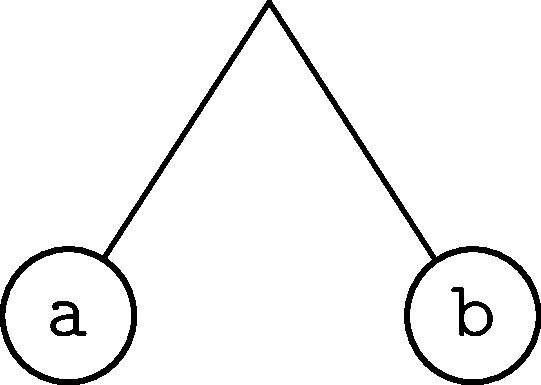
\includegraphics[width=0.135\textwidth]{lists-as-trees-1.pdf}}
  \hspace{0.1\textwidth}
  \subfigure[\texttt{(a b c)}]{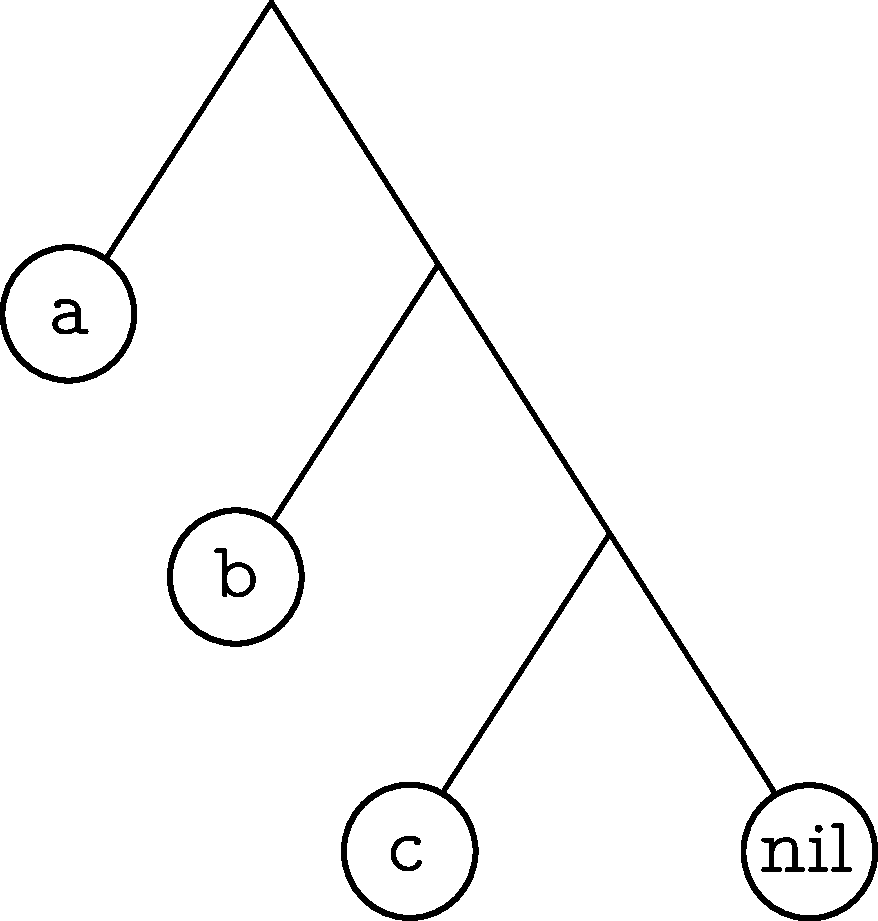
\includegraphics[width=0.21\textwidth]{lists-as-trees-2.pdf}}
  \hspace{0.1\textwidth}
  \subfigure[\texttt{(a b (c d))}]{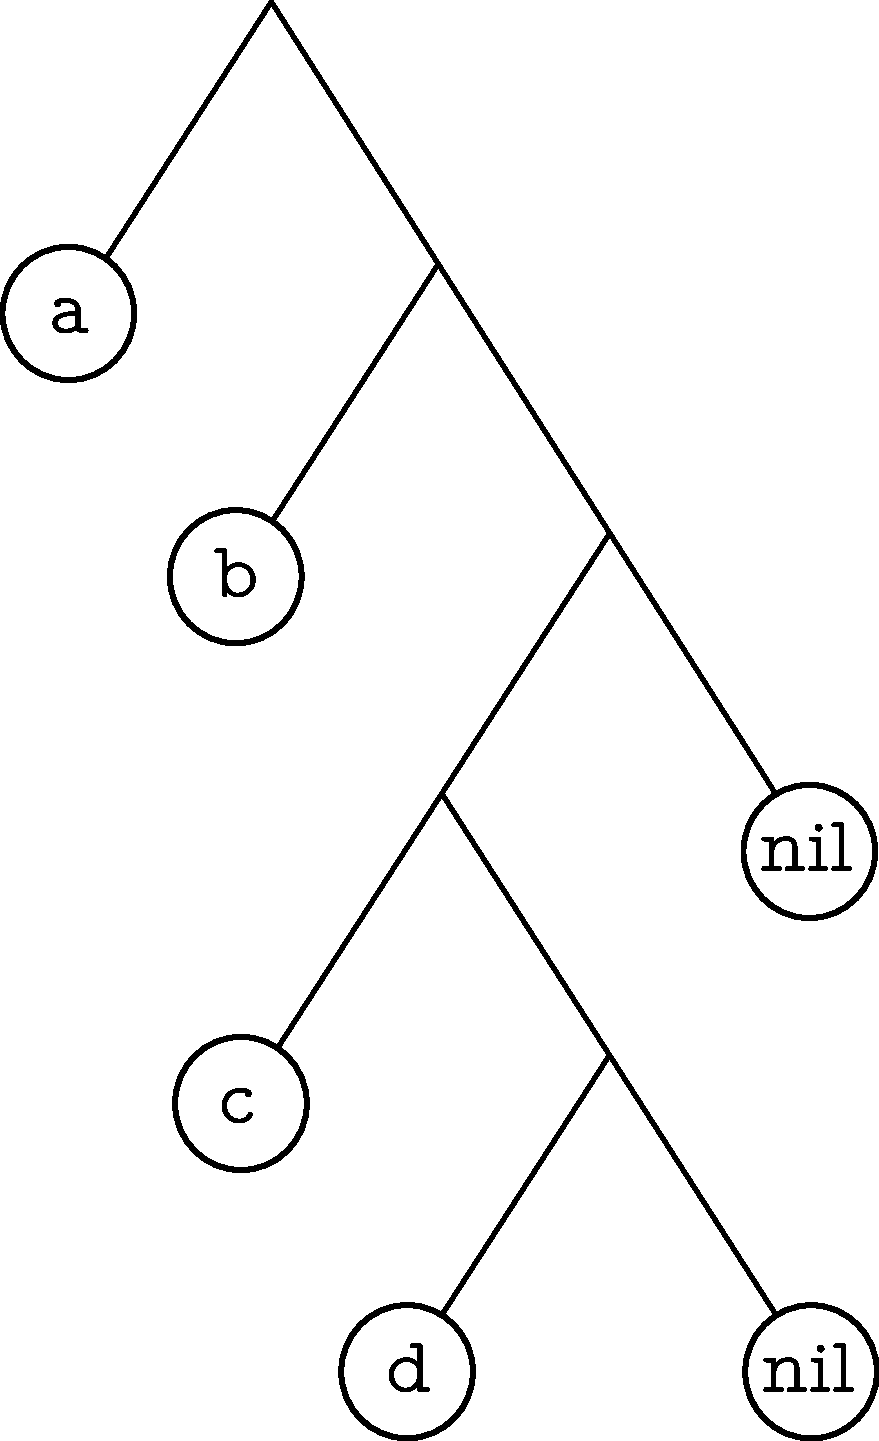
\includegraphics[width=0.21\textwidth]{lists-as-trees-3.pdf}}
  \caption{用列表表示的树}
  \label{fig:lists_as_trees}
\end{figure}

Lisp 的列表是一种全能型的数据结构\index{lists!uses for}。举例来说,列表能表示序列,集合,映射,数组,
以及树\index{trees 树}。目前有几种不同的方法来用列表表示树。
最常用的一种是把列表看作二叉树\index{lists!as binary trees},二叉树的左子树是~car,右子树则是~cdr。
(实际上,这往往就是列表的内部实现。) 图~\ref{fig:lists_as_trees}
中有三个例子,分别展示了列表以及它们所表示的树。其中,树上的每个内部节点
都对应着相应列表\index{dotted list}的\cons{}表示中的一个点,因而把列表看成下面的形式能更容易
理解这种的树型结构:
\begin{lstlisting}
    (a b c)     = (a . (b . (c . nil)))
    (a b (c d)) = (a . (b . ((c . (d . nil)) . nil)))
\end{lstlisting}
任意列表都可以看成一颗二叉树。同样的,Common Lisp 里也有其它一些成对的函数,它们之间的区别与~\texttt{copy-list}\index{copy-list@\texttt{copy-list}} 
和~\texttt{copy-tree}\index{copy-tree@\texttt{copy-tree}} 两者的区别类似。
前者把列表当作一个序列来处理,即如果碰到列表中含有子列表的情况,
那么子列表作为序列里的元素,是不会被复制的:
\begin{lstlisting}
> (setq x     '(a b)
        listx (list x 1))
((A B) 1)
> (eq x (car (copy-list listx)))
T
\end{lstlisting}
与之相对,\texttt{copy-tree} 会把列表当成树来拷贝,即把子列表视为子树,
所以子列表也一样会被复制:
\begin{lstlisting}
> (eq x (car (copy-tree listx)))
NIL
\end{lstlisting}
我们可以自己定义一个~\texttt{copy-tree},见下面的代码:
\begin{lstlisting}
(defun our-copy-tree (tree)
  (if (atom tree)
      tree
      (cons (our-copy-tree (car tree))
            (if (cdr tree) (our-copy-tree (cdr tree))))))
\end{lstlisting}
可以看出,上面的定义是一种常用模式的特例。(接下来,有些函数的写法会稍显
不自然,这是为了让这个模式变得更明显一些。) 不妨看看下面的例子,它能够
统计出一棵树里叶子节点\index{trees 树!leaves of 叶子}的数量:
\begin{lstlisting}
(defun count-leaves (tree)
  (if (atom tree)
      1
      (1+ (count-leaves (car tree))
          (or (if (cdr tree) (count-leaves (cdr tree)))
              1))))
\end{lstlisting}
一棵树上的叶子数会多于当它被表示成列表的形式时列表中原子的数量。
\begin{lstlisting}
> (count-leaves '((a b (c d)) (e) f))
10
\end{lstlisting}
而树用~\emph{\cons{}} 的形式来表示时,你可以注意到树上每个叶子都对应一个原子。
在\cons{}表示中,\texttt{((a b (c d)) (e) f)} 中有四个~\texttt{nil} 是在
列表表示中看不到的~(每对括弧都有一个),所以~\texttt{count-leaves} 的返回值是~10。

在上一章中,我们定义了几个用来操作树的\utility{}。比如说,\texttt{flatten}\index{flatten@\texttt{flatten}} 
(第~\pageref{fig:doubly-recursive_list_utilities} 页) 接受一颗树,
并返回一个含有树上所有原子的列表。换句话说,如果你传给~\texttt{flatten} 一个
嵌套列表,你所得到的返回列表和前面的列表形式相同,不过除了最外面那对之外,
其它的括弧都不见了:
\begin{lstlisting}
> (flatten '((a b (c d)) (e) f ()))
(A B C D E F)
\end{lstlisting}
这个函数也可以像下面那样定义~(尽管效率有点低):
\begin{lstlisting}
(defun flatten (tree)
  (if (atom tree)
      (mklist tree)
      (nconc (flatten (car tree))
             (if (cdr tree) (flatten (cdr tree))))))
\end{lstlisting}

最后,看一下~\texttt{rfind-if}\index{rfind-if@\texttt{rfind-if}},它是~\texttt{find-if}\index{find-if@\texttt{find-if}!version for trees} 的递归版本。
\texttt{rfind-if} 不仅能用在线性的列表上,而且对树也一样适用:
\begin{lstlisting}
(defun rfind-if (fn tree)
  (if (atom tree)
      (and (funcall fn tree) tree)
      (or (rfind-if fn (car tree))
          (if (cdr tree) (rfind-if fn (cdr tree))))))
\end{lstlisting}
为了让~\texttt{find-if} 的应用范围更广,使之能用于树结构,必须
在两者中择一: 让它仅仅搜索叶子节点,或是搜索整个子树。
我们的~\texttt{rfind-if}\note{73} 选择了前者,因而调用方就可以认为:
作为第一个参数传入的函数只会用在原子上:
\begin{lstlisting}
> (rfind-if (fint #'numberp #'oddp) '(2 (3 4) 5))
3
\end{lstlisting}

\texttt{copy-tree},\texttt{count-leaves},\texttt{flatten} 和~
\texttt{rfind-if},这四个函数的形式竟然如此相似。实际上,它们都是
某个原型函数的特例,这个原型函数被用来进行子树上的递归操作。和之前
对待~cdr 上递归的态度一样,我们不希望让这个原型默默无闻地埋没在代码当中,
相反,我们要写一个函数来产生这种原型函数的实例。

要得到原型本身,让我们先研究一下这些函数,找出哪些部分是不属于模式的。
从根本上来说,\texttt{our-copy-tree} 有两种情形:
\begin{enumerate}
\item 基本的情况下,函数直接把参数作为返回值返回
\item 在递归的时候,函数对左子树~(car) 的递归结果和右子树~(cdr) 
      的递归结果使用~\texttt{cons}
\end{enumerate}
因此,我们肯定可以通过调用一个有两个参数的构造函数,来表示~\texttt{our-copy-tree}:
\begin{lstlisting}
(ttrav #'cons #'identity)
\end{lstlisting}

图~\ref{fig:function_for_recursion_on_trees:ttrav} 中为~\texttt{ttrav} (``tree traverser'') 
的一种实现。在递归的情况下,我们传入的不是一个值,而是两个,一个对应左子树,
一个对应右子树。如果~\verb|base| 参数是个函数,那么将把当前叶子节点作为参数传给它。
在对线性列表进行递归操作时,基本情况的返回值总是~\verb|nil|,
不过在树结构的递归操作中,基本情况的值有可能是个更有意思的值,而且我们也许会需要用到它。

在~\verb|ttrav| 的帮助下,我们可以重新定义除~\verb|rfind-if| 之外前面提到的所有函数。
(这些函数在图~\ref{fig:functions_expressed_with_ttrav} 中可以找到。)
要定义~\verb|rfind-if|,需要更通用的树结构递归操作函数的生成器,
这种函数生成器能让我们控制递归调用发生的时机,以及是否继续递归。我们把一个函数作为传给~\verb|ttrav| 
的第一个参数,这个函数的参数将是递归调用的\emph{返回值}。对于通常的情形,
我们会改用另一个函数,让它接受两个闭包,闭包分别自行表示调用操作。这样,
就可以编写那些能自主控制递归过程的递归函数了。

\begin{figure}
\begin{lstlisting}
(defun ttrav (rec &optional (base #'identity))
  (labels ((self (tree)
                 (if (atom tree)
                     (if (functionp base)
                         (funcall base tree)
                         base)
                     (funcall rec (self (car tree))
                                  (if (cdr tree)
                                      (self (cdr tree)))))))
    #'self))
\end{lstlisting}
\caption{\label{fig:function_for_recursion_on_trees:ttrav}为在树上进行递归操作而设计的函数}
\index{ttrav@\texttt{ttrav}}
\end{figure}

\begin{figure}
\begin{lstlisting}
; our-copy-tree
(ttrav #'cons)

; count-leaves
(ttrav #'(lambda (l r) (+ l (or r 1))) 1)

; flatten
(ttrav #'nconc #'mklist)
\end{lstlisting}
\caption{\label{fig:functions_expressed_with_ttrav}用~\texttt{ttrav} 表示的函数}
\end{figure}

\begin{figure}
\begin{lstlisting}
(defun trec (rec &optional (base #'identiy))
  (labels
      ((self (tree)
             (if (atom tree)
                 (if (functionp base)
                     (funcall base tree)
                     base)
                 (funcall rec tree
                              #'(lambda ()
                                  (self (car tree)))
                              #'(lambda ()
                                  (if (cdr tree)
                                      (self (cdr tree))))))))
    #'self))
\end{lstlisting}
  \caption{\label{fig:function_for_recursion_on_trees:trec}为在树上进行递归操作而设计的函数}
  \index{trec@\texttt{trec}}
\end{figure}

用~\texttt{ttrav} 实现的函数通常会遍历整颗树。这样做对于像
~\texttt{count-leaves} 或者~\texttt{flatten} 这样的函数是没有问题的,
它们不管如何都会遍历全树。然而,我们需要~\texttt{rfind-if} 一发现
它所要找的元素就停止遍历。这个函数必须交给更通用的~\texttt{trec} 来生成,
见图~\ref{fig:function_for_recursion_on_trees:trec}。
\verb|trec| 的第二个参数应当是一个具有三个参数的函数,三个参数分别是:
当前的对象,以及两个递归调用。后两个参数将是用来表示对左子树和右子树进行
递归的两个闭包。使用~\verb|trec| 我们可以这样定义~\verb|flatten|:
\begin{lstlisting}
(trec #'(lambda (o l r) (nconc (funcall l) (funcall r)))
\end{lstlisting}
现在,我们同样可以把~\verb|rfind-if| 写成这样~(下面的例子用了~\verb|oddp|):
\begin{lstlisting}
(trec #'(lambda (o l r) (or (funcall l) (funcall r)))
      #'(lambda (tree) (and (oddp tree) tree)))
\end{lstlisting}

\section{何时构造函数}
\label{sec:when_to_build_functions}

很不幸,如果用构造函数,而非~sharp-quoted 的~lambda 表达式来表示
函数会在运行时让程序做一些不必要的工作。虽然~sharp-quoted 的~\lexpr
是一个常量,但是对构造函数的调用将会在运行时求值。如果你真的必须在运行
时执行这个调用,可能使用构造函数并非上策。不过,至少有的时候我们可以在事前就
调用这个构造函数。通过使用~\verb|#.|\index{\#.@\texttt{\#.}},即
~sharp-dot 读取宏,我们可以让
函数在读取期~(read-time) 就被构造出来。假设~\verb|compose| 和它的参数
在下面的表达式被读取时已经被定义了,那么我们可以这样写,举例如下:
\begin{lstlisting}
(find-if #.(compose #'oddp #'truncate) lst)
\end{lstlisting}
这样做的话,reader 就会对~\verb|compose| 的调用进行求值,求值得到的函
数则被作为常量安插在我们的代码之中。由于~\verb|oddp| 和~\verb|truncate| 
两者都是内置函数,所以在读取时对~\verb|compose| 进行估值可以被认为是
安全可行的,当然,前提是那个时候~\verb|compose| 自己已经加载了。

一般而言,由宏来完成函数复合或者合并,既简单容易,又提高了程序的性能。
这一点对函数拥有具有单独名字空间的~Common Lisp 来说尤其如此。
在介绍了宏的相关知识后,我们会在第~\ref{chap:macro_returning_functions} 章
故地重游,再次回到这一章中曾走到过的大多数山山水水,所不同的是,到那时
候你会骑上更纯种的宝马,配上更奢华的鞍具。

%%% Local Variables:
%%% coding: utf-8
%%% mode: latex
%%% TeX-master: "onlisp-cn"
%%% End:

%!TEX encoding = UTF-8 Unicode
% $Id: 6-functions_as_representation.tex 17 2014-03-09 13:05:41Z binghe $

\chapter{函数作为表达方式}
\label{chap:functions_as_representation}

通常说来,数据结构被用来\emph{描述事物}。可以用数组描述坐标变换,用树结
构表示命令的层次结构,而用图来表示铁路网。
在~Lisp 里,我们常会使用闭包\index{functions 函数!closures of}\index{functions 函数!as return values}\index{closures 闭包}作为表现形式。在闭包里,变量绑定可以
保存信息,也能扮演在复杂数据结构中指针\index{pointers 指针}的角色。
如果让一组闭包之间
共享绑定,或者让它们之间能相互引用\index{chains of closures},那么我们就可以创建混合型的对象类型,它同
时继承了数据结构和程序逻辑两者的优点。

其实在表象之下,共享绑定\emph{就是}指针。闭包只是让我们能在更高的抽象
层面上操作指针。通过用闭包来表示我们以往用静态数据结构表示的对
象,就往往可能得到更为优雅,效率更好的程序。

\section{网络}
\label{sec:networks}

闭包有三个有用的特性:它是动态的,拥有局部状态,而且我们可以创建
闭包的多个实例。那么带有局部状态的动态对象的多个拷贝能在什么地方一展身
手呢?答案是:和网络有关的程序。许多情况下,我们可以把网络中的节点表示
成闭包。闭包在拥有其局部状态的同时,它还能引用其它闭包。因而,一个表示
网络中节点的闭包是能够知道作为它发送数据目的地的其他几个节点~(闭包) 的。
换句话说,我们有能力把网络结构直接翻译成代码。

在本节和下一节里,我们会分别了解两种遍历网络的方法。首先我们会按照传统
的办法,即把节点定义成结构体\index{networks!representing},并用与之分离
的代码来遍历网络。接着,在下一节我们将会用一个统一的抽象模型来构造通用
功能的程序。

\begin{figure}
\begin{lstlisting}
> (run-node 'people)
Is the person a man?
>> yes
Is he living?
>> no
Was he American?
>> yes
Is he on a coin?
>> yes
Is the coin a penny?
>> yes
LINCOLN
\end{lstlisting}
\caption{\label{fig:session_of_20_questions}一轮~twenty questions 游戏}
\end{figure}

我们将选择一个最简单的应用作为例子:一个能运行~twenty questions\index{twenty questions}
\footnote{译者注:twenty questions 曾是一档国外很流行的电视智力节目,同
  时也是人工智能的重要题材。} 的程序。我们的网络将会是一棵二叉树。
每个非叶子节点都会含有一个是非题,并且根据对这个问题的回答,遍历过程
会在左子树或者右子树两者中择一,继续往下进行。叶子节点将会含有所有的返
回值。当遍历过程遇到叶子节点时,叶子节点的值会被作为遍历过程的返回值返
回。如图~\ref{fig:session_of_20_questions} 所示,是程序运行一轮~twenty
questions 的样子。

\begin{figure}
\begin{lstlisting}
(defstruct node  contents yes no)

(defvar *nodes* (make-hash-table))

(defun defnode (name conts &optional yes no)
  (setf (gethash name *nodes*)
        (make-node :contents conts
                   :yes      yes
                   :no       no)))
\end{lstlisting}
\caption{\label{fig:representation_and_definition_of_nodes}节点的表示方法及其定义
}
\end{figure}

从习惯的办法着手,可能就是先定义某种数据结构来表示节点。节点应该包含这
几样信息:它是否是叶子节点;如果是的话,那返回值是什么,倘若不是,要问
什么问题;还有与答案对应的下个节点是什么样的。
图~\ref{fig:representation_and_definition_of_nodes} 里定义了一个信息足
够详尽的数据结构。它的设计目标是让数据所占的空间最小化。\texttt{contents} 字
段中要么是问题要么是返回值。如果该节点不是叶子节点,那么~\texttt{yes}
和~\texttt{no} 字段会告诉我们与问题的答案对应的去向;如果节点是个叶子节
点,我们自然会知道这一点,因为这些字段会是空的。全局
的~\texttt{*nodes*} 是一个哈希表,在表中,我们会用节点的名字来索引节点。
最后,\texttt{defnode} 会新建一个节点~(两种节点都可以),并把它保存
到~\texttt{*nodes*} 中。有了这些原材料,我们就可以定义树的第一个节点了:
\begin{lstlisting}
(defnode 'people "Is the person a man?"
         'male 'female)
\end{lstlisting}
图~\ref{fig:sample_network} 中所示的网络正好足够我们运
行~\ref{fig:session_of_20_questions} 中所示的一轮游戏。

\begin{figure}
\begin{lstlisting}
(defnode 'people "Is the person a man?" 'male 'female)

(defnode 'male "Is he living?" 'liveman 'deadman)

(defnode 'deadman "Was he American?" 'us 'them)

(defnode 'us "Is he on a coin?" 'coin 'cidence)

(defnode 'coin "Is the coin a penny?" 'penny 'coins)

(defnode 'penny 'lincoln)
\end{lstlisting}
\caption{\label{fig:sample_network}作为样例的网络}
\end{figure}

\begin{figure}
\begin{lstlisting}
(defun run-node (name)
  (let ((n (gethash name *nodes*)))
    (cond ((node-yes n)
           (format t "~A~%>> " (node-contents n))
           (case (read)
             (yes (run-node (node-yes n)))
             (t   (run-node (node-no n)))))
          (t (node-contents n)))))
\end{lstlisting}
  \caption{\label{fig:function_for_traversing_networks}用来遍历网络的函数}
\end{figure}

现在,我们要做的就是写一个能遍历这个网络的函数了,这个函数应该打印出问
题,并顺着答案所指示的路径走下去。函数的名字是~\texttt{run-node},如
图~\ref{fig:function_for_traversing_networks} 所示。给出一个名字,
我们就根据名字找到对应的节点。如果该节点不是叶子节点,
就把~\texttt{contents} 作为问题打印出来,按照答案不同,我们继续顺着
两条可能的途径之一继续遍历。如果该节点是叶子节点,\texttt{run-node} 
会径直返回~\texttt{contents}。使用图~\ref{fig:sample_network} 中
定义的网络,这个函数就能生成图~\ref{fig:session_of_20_questions} 
中的输出信息。


\section{编译后的网络}
\label{sec:compiling_networks}
\index{compilation 编译!of networks 网络}

在上一节,我们编写了一个使用网络的程序,也许使用任何一种语言都能写出
这样的程序。的确,这个程序太简单了,看上去似乎很难把它写成另一个模样。
但是事实上,我们可以把程序打理得更简洁一些。

\begin{figure}
\begin{lstlisting}
(defvar *nodes* (make-hash-table))

(defun defnode (name conts &optional yes no)
  (setf (gethash name *nodes*)
        (if yes
            #'(lambda ()
                (format t "~A~%>> " conts)
                (case (read)
                  (yes (funcall (gethash yes *nodes*)))
                  (t   (funcall (gethash no  *nodes*)))))
            #'(lambda () conts))))
\end{lstlisting}
  \caption{\label{fig:a_netwok_compiled_into_closures}编译成闭包形式的网络}
\end{figure}

图~\ref{fig:a_netwok_compiled_into_closures} 就是明证。这是让我们的网
络运行起来所需要的所有代码。在这里,不再把节点定义成一个结构,也没有用
一个单独的函数来遍历这些节点,而是把节点表示成闭包\index{networks!representing}。原来保存在数据结构里的数据现在栖身于闭包里的变量绑定中。没有必要运
行~\texttt{run-node} 了,它已经隐含在了节点自身里面。要启动遍历过程,
只消~funcall 一下起始的那个节点就行了:
\begin{lstlisting}
(funcall (gethash 'people *nodes*))
Is the person a man
>>
\end{lstlisting}
自此,接下来的人机对话就和上个版本的实现一样了。

借助把节点都表示成闭包的方式,我们得以将~twenty questions 网络完全转化
成代码~(而非数据)。正如我们所看到的,程序代码必须在运行时按照名字来查找
节点函数。然而,如果我们确信网络在运行的时候不会重新定义,那就可以
更进一步:让节点函数直接调用它们的下一站目标函数,而不必再动用
哈希表了。

\begin{figure}
\begin{lstlisting}
(defvar *nodes* nil)

(defun defnode (&rest args)
  (push args *nodes*)
  args)

(defun compile-net (root)
  (let ((node (assoc root *nodes*)))
    (if (null node)
        nil
      (let ((conts (second node))
            (yes (third node))
            (no (fourth node)))
        (if yes
            (let ((yes-fn (compile-net yes))
                  (no-fn  (compile-net no)))
              #'(lambda ()
                  (format t "~A~%>> " conts)
                  (funcall (if (eq (read) 'yes)
                               yes-fn
                               no-fn))))
            #'(lambda () conts))))))
\end{lstlisting}
  \caption{\label{fig:compilation_with_static_reference}使用静态引用的编译过程}
\end{figure}

如图~\ref{fig:compilation_with_static_reference} 所示,是新版的程序代码。
现在,\texttt{*node*} 从哈希表改成了一个列表。像以前一样,所有的节点还是
用~\texttt{defnode} 定义的,不过定义时并不会生成闭包。在定义好所有的节
点之后,我们就调用~\texttt{compile-net} 来一次性地编译整个网络。
这个函数递归地进行处理,一直往下,直至树的叶子节点,在递归过程层层返回
时,每一步都返回了两个目标函数对应的节点~(或称函数),而不仅仅是给出它们
的名字。\footnote{这个版本的程序假定程序中的网络是一种树结构,这个前提
  对这个应用来说肯定是成立的。} 当最外面的~\texttt{compile-net} 调用返
回时,它给出的函数将表示一个我们所需的那部分网络。
\begin{lstlisting}
> (setq n (compile-net 'people))
#<Compiled-Function BF3C06>
> (funcall n)
Is the person a man?
>>
\end{lstlisting}
注意到,\texttt{compile-net} 进行的编译有两层含义。按照通常编
译的含义,它把网络的抽象表示翻译成了代码。更进一层,如果~\texttt{compile-net} 
自身被编译的话,那它就会返回编译后的函数。(见第~\pageref{page:compiled_function} 页)
\label{page:new-language-compiler}

在编译好网络之后,由~\texttt{defnode} 构造的列表就没用了。
如果切断列表与程序的联系~(例如将~\texttt{*nodes*} 设为~\texttt{nil}),
垃圾收集器\index{garbage 垃圾!collection 回收}就会回收它。

\section{展望}
\label{sec:looking_forward}

有许多涉及网络的程序都能通过把节点编译成闭包的形式来实现。闭包作为数据
对象,和各种数据结构一样能用来表现事物的属性。这样做需要一些和习惯相
左的思考方式,但是作为回报的是更为迅速,更为优雅的程序。

宏在相当程度上将有助于我们把闭包用作一种表达方式。``用闭包来表示
'' 是~``编译'' 的另外一种说法。而且由于宏是在编译时完成它们的工作的,
因而它们理所应当地就是这种技术的最佳载体。在介绍了宏技术之后,
第~\ref{chap:parsing_with_atns} 章和第~\ref{chap:prolog} 章里会
呈上更大规模的程序,这些程序将会使用这里曾用过的方法写成。

%%% Local Variables:
%%% coding: utf-8
%%% mode: latex
%%% TeX-master: "onlisp-cn"
%%% End:

%!TEX encoding = UTF-8 Unicode
% $Id: 7-macros.tex 17 2014-03-09 13:05:41Z binghe $

\chapter{宏}
\label{chap:macros}
\index{macros 宏}
\index{macros 宏|seealso {backquote, read-macro, symbol-macros}}

Lisp 中,宏的特性让你能用变换的方式定义操作符。宏定义\index{macros 宏!defining}在本质上,是能
生成~Lisp 代码的函数\pozhehao{}一个能写程序的程序。这一小小开端引发了巨大 
的可能性,同时也伴随着难以预料的风险。
第~\ref{chap:macros}--\ref{chap:other_macro_pitfalls} 章将带你走入宏的
世界。本章会解释宏如何工作,介绍编写和调试它们的技术,然后分析一些宏风
格中存在的问题。

\section{宏是如何工作的}
\label{sec:how_macros_work}

由于我们可以调用宏并得到它的返回值,因此宏往往被人们和函数联系在一起。宏定义有时和
函数定义相似,而且不严谨地说,被人们称为~``内置函数'' 的~\texttt{do} 其实就是一
个宏。但如果把两者过于混为一谈,就会造成很多困惑。宏和常规函数的工作方式
截然不同,并且只有知道宏为何不同,以及怎样不同才是用好它们的关键。一个函数只产
生结果,而宏却产生\emph{表达式}\pozhehao{}当它被求值时,才会产生结果。

要入门,最好的办法就是直接看个例子。假设我们想要写一个
宏~\texttt{nil!},它把实参设置为~\verb|nil|。让~\verb|(nil! x)|
和~\texttt{(setq x nil)} 的效果一样。我们完成这个功能的方法
是:把~\texttt{nil!} 定义成宏,让它来把前一种形式的实例变成后一
种形式的实例。
\begin{lstlisting}
> (defmacro nil! (var)
    (list 'setq var nil))
NIL!
\end{lstlisting}
\index{defmacro@\texttt{defmacro}}
用汉语转述的话,这个定义相当于告诉~Lisp: ``无论何时,只要看到形
如~\texttt{(nil! $var$)} 的表达式,请在求值之前先把它转化
成~\texttt{(setq $var$ nil)} 的形式。''

宏产生的表达式将在调用宏的位置求值。宏调用是一个列表,列表的第一个元素是
宏的名称。当我们把宏调用~\texttt{(nil! x)} 输入到~toplevel 的时候发生了
什么? Lisp 首先会发觉~\texttt{nil!} 是个宏的名字,然后
\begin{enumerate}
 \item 按照上述定义的要求构造表达式,接着
 \item 在调用宏的地方求值该表达式。
\end{enumerate}

构造新表达式的那一步被称为\emph{宏展
  开~(macroexpansion)}\index{macros 宏!expansion of}。Lisp 查
找~\texttt{nil!} 的定义,其定义展示了如何为宏调用构建一个即将取代它的表
达式。和函数一样,\texttt{nil!} 的定义也应用到了宏调用传给它
的\emph{表达式}参数上。它返回一个三元素列表,这三个元素分别是:
\texttt{setq}、作为参数传递给宏的那个表达式,以及~\texttt{nil}。在本例
中,\texttt{nil!} 的参数是~\texttt{x},宏展开式是~\texttt{(setq x
  nil)}。

宏展开之后是第二步:\emph{求值~(evaluation)}。Lisp 求值宏展开
式~\texttt{(setq x nil)} 时就好像是你原本就写在那儿的一样。求值并不总是
立即发生在展开之后,不过在~toplevel 下的确是这样的。一个发生在函数定
义里的宏调用将在函数编译时展开\index{macros 宏!compiled}, 但展开式\pozhehao{}或者说它产生的对象代
码\pozhehao{}要等到函数被调用时才会求值。

如果把宏的展开和求值分清楚,你遇到的和宏有关的困难,或许有很多就能避免。
当编写宏的时候,要清楚哪些操作是在宏展开期进行的\index{macros 宏!expansion of!time of},而哪些操作是在求值期
进行的,通常,这两步操作的对象截然不同。宏展开步骤处理的是表达式,而求
值步骤处理的则是它们的值。

有些宏的展开过程比~\texttt{nil!} 的情况更复杂。\texttt{nil!} 的展开
式只是调用了一下内置的~special form,但往往一个宏的展开式可能会是另一个宏
调用,就好像是一层套一层的俄罗斯套娃。在这种情况下,宏展开就会继续抽丝剥
茧直到获得一个没有宏的表达式。这一步骤中可以经过任意多次的展开操作,一
直到最终停下来。

尽管有许多语言也提供了某种形式的宏,但~Lisp 宏却格外强大。在编译~Lisp
文件时,解析器先读取源代码,然后将其输出送给编译器。这里有个天才的手
笔:解析器的输出由\emph{~Lisp 对象的列表}组成。通过使用宏,我们可以操
作这种处于解析器和编译器之间的中间状态的程序。如果必要的话,这些操作可
以无所不包。一个生成展开式的宏拥有~Lisp 的全部威力,可任其驱驰。事实
上,宏是货真价实的~Lisp 函数\pozhehao{}那种能返回表达式的函数。虽
然~\texttt{nil!} 的定义中只是调用了一下~\texttt{list},但其他宏里可能会
驱动整个子程序来生成其展开式。

有能力改变编译器所看到的东西,差不多等同于能够对代码进行重写。所以我们就可以为语言
增加任何构造,只要用变换的方法把它定义成已有的构造。

\section{\bq{}~(backquote)}
\label{sec:backquote}

\bq{}~(backquote)\index{backquote@backquote (\texttt{`}) \bq{}} 是引用~(quote)\index{quote@\texttt{quote}} 的特别
版本,它可以用来创建~Lisp 表达式的模板。\bq{}最常见的用途之一是用在宏定义里。

\bq{}字符``\texttt{`}''得名的原因是:它和通常的引号``\texttt{'}''相似,只
不过方向相反。当单独把\bq{}作为表达式前缀的时候,它的行为和引号一样:
\begin{equation*}
  \mbox{\texttt{`(a b c)} 等价于~\texttt{'(a b c)}.}
\end{equation*}

%% xxx
只有在\bq{}和\comma{}``\texttt{,}''\index{,@\texttt{,}},以及~comma-at
``\texttt{,@}''一同出现时才变得有用。如果说\bq{}创建了一个模
板,那么\comma{}就在\bq{}中创建了一个~slot。一个\bq{}列表等价于将其元素
引用起来,调用一次~\texttt{list}。也就是,
\begin{equation*}
  \mbox{\texttt{`(a b c)} 等价于~\texttt{(list 'a 'b 'c)}.}
\end{equation*}
在\bq{}的作用域里,\comma{}要求~Lisp:“把引用关掉”。当\comma{}出现在列表
元素前面时,它的效果就相当于取消引用,让~Lisp 把那个元素按原样放在那里。所以
\begin{equation*}
  \mbox{\texttt{`(a ,b c ,d)} 等价于~\texttt{(list 'a b 'c d)}.}
\end{equation*}
插入到结果列表里的不再是符号~\texttt{b},取而代之的是它的值。无论\comma{}在嵌套列表里
的层次有多深,它都仍然有效,
\begin{lstlisting}
> (setq a 1 b 2 c 3)
3
> `(a ,b c)
(A 2 C)
> `(a (,b c))
(A (2 C))
\end{lstlisting}
而且它们也可以出现在引用的列表里,或者引用的子列表里:
\begin{lstlisting}
> `(a b ,c (',(+ a b c)) (+ a b) 'c '((,a 'b)))
(A B 3 ('6) (+ A B) 'C '((1 'B)))
\end{lstlisting}

一个\comma{}能抵消一个\bq{}的效果,所以\comma{}在数量上必须和\bq{}匹配。如果某个
操作符出现在\comma{}的外层,或者出现在包含\comma{}的那个表达式的外层,那么我们说
该操作符\emph{包围}了这个\comma{}。例如在~\texttt{`(,a ,(b `,c))} 中,
最后一个\comma{}就被
前一个\comma{}和两个反引号所包围。通行的规则是:一个被~$n$ 个\comma{}包围的\comma{}必须被至少
~$n+1$ 个反引号所包围。很明显,由此可知:\comma{}不能出现在\bq{}的表达式的外面
。只要遵守上述规则,就可以嵌套使用\bq{}和\comma{}。下面的任何一个表达式如果输入到
~toplevel 下都将造成错误:
\begin{center}
  \verb|,x|\qquad\verb|`(a ,,b c)|\qquad\verb|`(a ,(b ,c) d)|\qquad\verb|`(,,`a)|
\end{center}
嵌套的\bq{}只有在宏定义的宏里才可能会用到。
第~\ref{chap:macro-defining_macros} 章将讨论这两个主题。

\bq{}通常被用来创建列表。\footnote{\bq{}也可以用于创建向量~(vector)\index{vectors 向量!creating with backquote 用\bq{}来创建},不过这个
用法很少在宏定义里出现。}任何用\bq{}生成的列表也都可以用~\texttt{list} 和
普通的引用来实现。使用\bq{}的好处只是在于它改进了表达式的可读性,因为反
引用的表达式和它将生成的表达式很相似。在前一章里我们把~\texttt{nil!} 定义成:
\begin{lstlisting}
(defmacro nil! (var)
  (list 'setq var nil))
\end{lstlisting}
借助\bq{},这个宏可以定义成:
\begin{lstlisting}
(defmacro nil! (var)
  `(setq ,var nil))
\end{lstlisting}
在本例中,是否使用\bq{}的差别还不算太大。不过,随着宏定义长度的增加,\bq{}也会变得愈加重要。
图~\ref{fig:a_macro_defined_with_and_without_backquote} 包含了两个
~\texttt{nif}\label{mac:nif}
可能的定义,这个宏实现了三路数值条件选择。
\footnote{这个宏的定义稍微有些不自然,这是为了避免使用~gensym。
在第~\pageref{fig:macros_for_conditional_evaluation} 页上有一个更好的定义。}

\begin{figure}
使用\bq{}:
\begin{lstlisting}
(defmacro nif (expr pos zero neg)
  `(case (truncate (signum ,expr))
     (1 ,pos)
     (0 ,zero)
     (-1 ,neg)))
\end{lstlisting}
不使用\bq{}:
\begin{lstlisting}
(defmacro nif (expr pos zero neg)
  (list 'case
     (list 'truncate (list 'signum expr))
     (list 1 pos)
     (list 0 zero)
     (list -1 neg)))
\end{lstlisting}
\index{nif@\texttt{nif}}
\index{signum@\texttt{signum}}
\caption{\label{fig:a_macro_defined_with_and_without_backquote}一个使用和不使
用\bq{}的宏定义。}
\end{figure}

首先,第一个参数会被求值成数字。然后会根据这个数字的正负、是否为零,来决定第二、第
三和第四个参数中哪一个将被求值:

\begin{lstlisting}
> (mapcar #'(lambda (x)
              (nif x 'p 'z 'n))
          '(0 2.5 -8))
(Z P N)
\end{lstlisting}

图~\ref{fig:a_macro_defined_with_and_without_backquote} 中的两个定义分
别定义了同一个宏,但是前者使用的是\bq{},而后者则通过显式调
用~\texttt{list} 来构造它的展开式。以~\texttt{(nif x 'p 'z
  'n)} 为例,从第一个定义中很容易就能看出来,这个表达式会展开成
\begin{lstlisting}
(case (truncate (signum x))
  (1 'p)
  (0 'z)
  (-1 'n))
\end{lstlisting}
因为这个宏定义体的模样就和它生成的宏展开式差不多。要想理解不使用\bq{}的第
二个版本,你将不得不在脑海中重演一遍展开式的构造过程。

comma-at,即``\texttt{,@}\index{,"@@\texttt{,"@}}'',是\comma{}的变
形,其行为和\comma{}相似,但有一点不同: comma-at 不像\comma{}那样仅仅把
表达式的值插入到所在的位置,而是把表达式\emph{拼接}\index{splicing 拼接}进去。拼接这个操作
可以这样理解:在插入的同时,剥去被插入对象最外层的括号:
\begin{lstlisting}
> (setq b '(1 2 3))
(1 2 3)
> `(a ,b c)
(A (1 2 3) C)
> `(a ,@b c)
(A 1 2 3 C)
\end{lstlisting}

\comma{}导致列表~\texttt{(1 2 3)} 被插入到~\texttt{b} 所在的位置,而~comma-at~把列表中的元素
插入到那里。对于~comma-at~的使用,还另有限制:
\begin{enumerate}
\item 为了确保其参数可以被拼接,comma-at~必须出现在序列~(sequence)
\footnote{译者注:序列~(sequence) 是~Common Lisp 标准定义的数据类型,它的两个子
类型分别是列表~(list) 和向量~(vector)。}中。形如~\texttt{`,@b} 的说法是错误的,因为无处
可供~\texttt{b} 的值进行拼接。
\item 要进行拼接的对象必须是个列表,除非它出现在列表最后。
表达式~\texttt{`(a ,@1)} 将被求值成~\texttt{(a . 1)},但如果尝试将
原子\footnote{译者注:原子~(atom) 也是~Common Lisp 标准定义的数据类型,所
有不是列表的~Lisp 对象都是原子,包括向量~(vector) 在内。}~(atom) 拼接到列表
的中间位置,例如~\texttt{`(a ,@1 b)},将导致一个错误。
\end{enumerate}

comma-at~一般用在接受不确定数量参数的宏里,以及将这些参数传给同样接受不确定
数量参数的函数和宏里。这一情况通常广泛用于实现隐式的块~(block)。Common Lisp
提供几种将代码分组到块的操作符,包括~\texttt{block}、\texttt{tagbody}, 以及
~\texttt{progn}。这些操作符很少直接出现在源代码里;它们一般不显山露水\pozhehao{}
而是藏身在宏的背后。

隐式块出现在任何一个带有表达式\emph{体}\index{body (of expressions) 体~(表达式)}的内置宏里。例如~\texttt{let} 和
~\texttt{cond} 里都有隐式的~\texttt{progn} 存在。做这种事情的内建宏里,最简单的
一个可能要算~\texttt{when} 了:
\begin{lstlisting}
(when (eligible obj)
  (do-this)
  (do-that)
  obj)
\end{lstlisting}
如果~\texttt{(eligible obj)} 返回真,那么其余的表达式将会被求值,并且整个
~\texttt{when} 表达式会返回其中最后一个表达式的值。下面是一个使用~comma-at 的示例,
它是~\texttt{when} 的一种可能的实现:
\begin{lstlisting}
(defmacro our-when (test &body body)
  `(if ,test
       (progn
         ,@body)))
\end{lstlisting}
这一定义使用了一个~\texttt{\&body}\index{body@\texttt{\&body}} 参数~(它和~\texttt{\&rest}\index{rest@\texttt{\&rest} parameters} 功能相同,只有美观
输出的时候不太一样) 来接受可变数量的参数,然后一个~comma-at~将它们拼接到一个
~\texttt{progn} 表达式里。在上述调用的宏展开式里,宏调用体里面的三个表达式将
出现在单个~\texttt{progn} 中:
\begin{lstlisting}
(if (eligible obj)
    (progn (do-this)
           (do-that)
           obj))
\end{lstlisting}

多数需要迭代处理其参数的宏都采用类似方式拼接它们。

comma-at~的效果也可以不用\bq{}实现。例如,表达式~\verb|`(a ,@b c)| 就和
~\verb|(cons 'a (append b (list 'c)))| 等价。之所以用上~comma-at,
只是为了改进这种由表达式生成的表达式的可读性。

宏定义~(通常) 生成列表。尽管宏展开式可以用函数~\verb|list| 来生成,但\bq{}的
列表模板可以令这一任务更为简单。用~\verb|defmacro| 和\bq{}定义的宏,在形式
上和用~\verb|defun| 定义的函数非常相似。只要不被这种相似性误导,\bq{}
就能让宏定义既容易书写也方便阅读。

由于\bq{}经常出现在宏定义里,以致于人们有时误以为\bq{}是~\verb|defmacro| 的一部分。
关于\bq{}的最后一件要记住的事情,是它有自己存在的意义,这跟它在宏定义中的角色无关。
你可以在任何需要构造序列的场合使用\bq{}:
\begin{lstlisting}
(defun greet (name)
  `(hello ,name))
\end{lstlisting}

\section{定义简单的宏}
\label{sec:defining_simple_macros}
\index{macros 宏!simple}

在编程领域,最快的学习方式通常是尽快地开始实践。完全理论上的理解可以稍后再说。
因此本章介绍一种可以立即开始编写宏的方法。虽然该方法的适用范围很窄,但在这个
范围内却可以高度机械化地实现。(如果你以前写过宏,可以跳过本节。)

下面举个例子,让我们考虑一下如何写出~Common Lisp 内置函
数~\verb|member|\index{member@\texttt{member}} 的
变形。\verb|member| 缺省用~\verb|eql| 来判断等价与否。如果你想要
用~\verb|eq| 来判断是否等价,你就必须显式写成这样:
\begin{lstlisting}
(member x choices :test #'eq)
\end{lstlisting}

如果常常这样做,那我们可能会想要写一个~\verb|member| 的变形,让它总是
使用~\verb|eq|。有些早期的~Lisp 方言就有这样的一个函数,叫
做~\verb|memq|\index{memq@\texttt{memq}}:
\begin{lstlisting}
(memq x choices)
\end{lstlisting}
通常应该将~\texttt{memq} 定义为内联~(inline) 函数,但为了举例子,我们会
让它以宏的面目出现。

\begin{figure}
  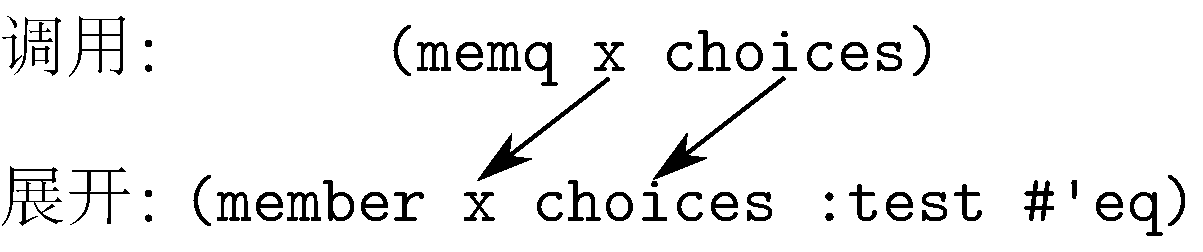
\includegraphics[width=.46\textwidth]{memq.pdf}
  \caption{\label{fig:diagram_used_in_writing_memq}用于写~\texttt{memq} 的图示}
\end{figure}

方法如下:从你想要定义的这个宏的一次典型调用开始。先把它写在纸上,然后下面写上
它应该展开成的表达式。图~\ref{fig:diagram_used_in_writing_memq} 给出了两个这样
的表达式。通过宏调用,构造出你这个宏的参数列表,同时给每个参数命名。
这个例子中有两个实参,所以我们将会有两个形参,把它们叫做~\verb|obj|
和~\verb|lst|:
\begin{lstlisting}
(defmacro memq (obj lst)
\end{lstlisting}
现在回到之前写下的两个表达式。对于宏调用中的每个参数,画一条线把它和它
在展开式里出现的位置连起来。图~\ref{fig:diagram_used_in_writing_memq} 中有
两条并行线。为了写出宏的实体,把你的注意力转移到展开式。让主体以\bq{}开头。
现在,开始逐个表达式地阅读展开式。每当发现一个括号,如果它不是宏调用中实参
的一部分,就把它放在宏定义里。所以紧接着\bq{}会有一个左括号。对于展开式里的每个
表达式
\begin{enumerate}
\item 如果没有线将它和宏调用相连,那么就把表达式本身写下来。
\item 如果存在一条跟宏调用中某个参数的连接,就把出现在宏参数列表的对应位置的那个
  符号写下来,前置一个\comma{}。
\end{enumerate}
由于第一个元素~\verb|member| 上没有连接,所以我们照原样使用~\verb|member|:
\begin{lstlisting}
(defmacro memq (obj lst)
  `(member
\end{lstlisting}
不过,\verb|x| 上有一条线指向源表达式中的第一个实参,所以我们在宏的主体
中使用第一个参数,带一个\comma{}:
\begin{lstlisting}
(defmacro memq (obj lst)
  `(member ,obj
\end{lstlisting}
以这种方式继续进行,最后完成的宏定义是:
\begin{lstlisting}
(defmacro memq (obj lst)
  `(member ,obj ,lst :test #'eq))
\end{lstlisting}

\begin{figure}
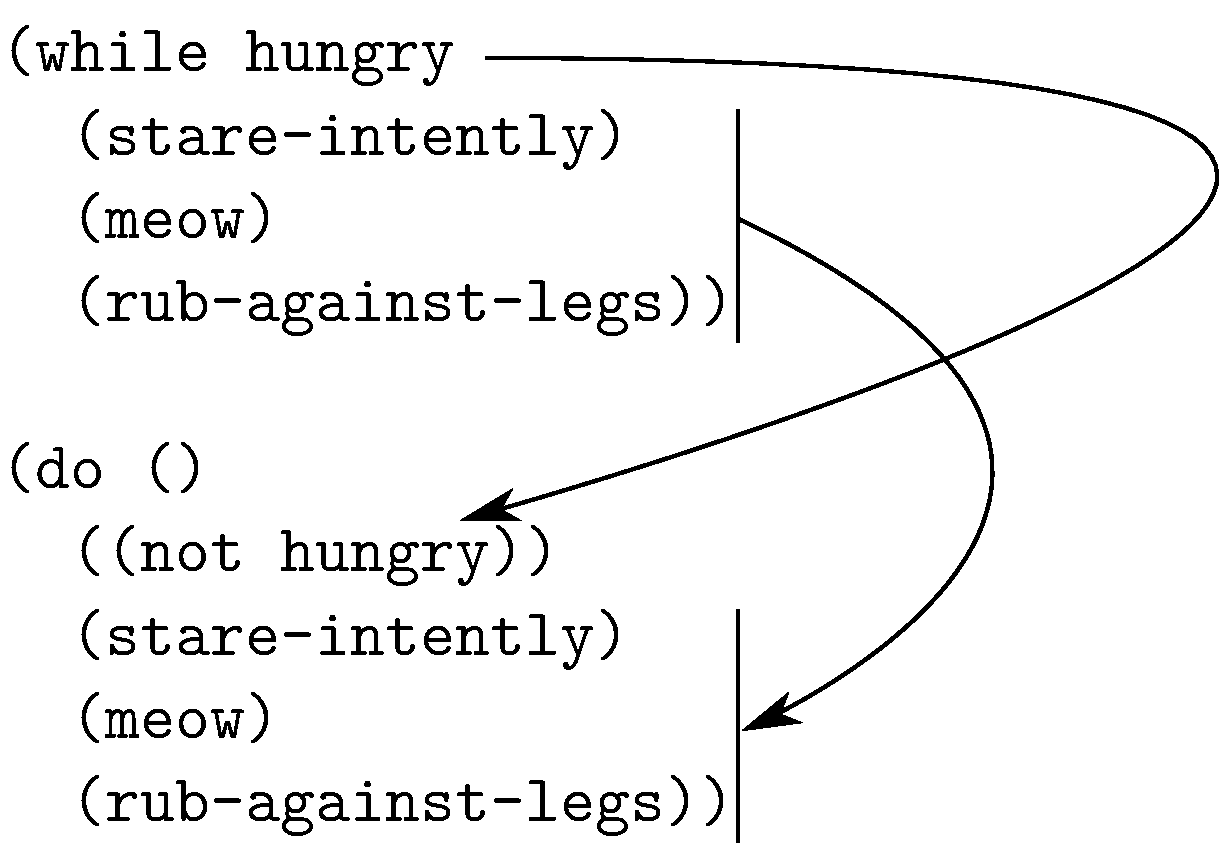
\includegraphics[width=.46\textwidth]{while.pdf}
\caption{\label{fig:diagram_used_in_writing_while}用于写~\texttt{while} 的图示}
\end{figure}

到目前为止,我们写出的宏,其参数个数只能是固定的。现在假设我们打算写一
个~\verb|while| 宏,它接受一个条件表达式和一个代码体,然后循环执行代
码直到条件表达式返回真。图~\ref{fig:diagram_used_in_writing_while} 含有
一个描述猫的行为的~\verb|while| 循环示例。

要写出这样的宏,我们需要对我们的技术稍加修改。和前面一样,先写一个宏
调用作为毛坯。然后,以它为基础,构造宏的形参列表,其中,在想要接受任意多
个参数的地方,以一个~\verb|&rest| 或~\verb|&body| 形参作结:
\begin{lstlisting}
(defmacro while (test &body body)
\end{lstlisting}
现在,在宏调用的下面写出目标展开式,并且和之前一样,画线把宏调用的形参和
它们在展开式中的位置连起来。然而,当你碰到一个系列形参,而且它们会
被~\verb|&rest| 或~\verb|&body| 实参吸收时,就要把它们当成一组
处理,并只用一条线来连接整个参数序列。
图~\ref{fig:diagram_used_in_writing_while} 给出了最后的图示。

为了写出宏定义的主体,按之前的步骤处理表达式。在前面给出的两条规则之外,
我们还要加上一条:
\begin{enumerate}
\setcounter{enumi}{2}
\item 如果在一系列展开式中的表达式和宏调用里的一系列形参之间存在联系,那么
  就把对应的~\verb|&rest| 或~\verb|&body| 实参记下来,在前面加上~comma-at。
\end{enumerate}
于是宏定义的结果将是:\label{macro:while}
\begin{lstlisting}
(defmacro while (test &body body)
  `(do ()
       ((not ,test))
     ,@body))
\end{lstlisting}
要想构造带有表达式\emph{体}\index{body (of expressions) 体~(表达式)}的宏,就必须有参数充当打包装箱的角色。这里宏调用中的
多个参数被串起来放到~\verb|body| 里,然后在~\verb|body| 被拼接进展开式时,再把它
拆散开。

用本章所述的这个方法,我们能写出最简单的宏\pozhehao{}这种宏只能在参数位置上做
文章。但是宏可以比这做的多得多。第~\ref{sec:macros_as_programs} 章将会举
一个例子,这个例子无法用简单的\bq{}列表表达,并且为了生成展开式,例子中的
宏成为了真正意义上的程序。

\section{测试宏展开}
\label{sec:testing333_macroexpansion}

宏写好了,那我们怎么测试它\index{macros 宏!testing 测
  试}呢?像~\verb|memq| 这样的宏,它的结构较简单,只消看看它的代码就
能弄清其行为方式。而当编写结构更复杂的宏时,我们必须有办法检查它们展开
之后正确与否。

\begin{figure}
\begin{lstlisting}
> (defmacro while (test &body body)
    `(do ()
         ((not ,test))
       ,@body))
WHILE

> (pprint (macroexpand '(while (able) (laugh))))

(BLOCK NIL
  (LET NIL
    (TAGBODY
      #:G61
      (IF (NOT (ABLE)) (RETURN NIL))
      (LAUGH)
      (GO #:G61))))
T
> (pprint (macroexpand-1 '(while (able) (laugh))))

(DO NIL
    ((NOT (ABLE)))
  (LAUGH))
T
\end{lstlisting}
\caption{\label{fig:a_macro_and_two_depths_of_expansion}一个宏和它的两级展开}
\end{figure}

图~\ref{fig:a_macro_and_two_depths_of_expansion} 给出了一个宏定义和用
来查看其展开式的两个方法。内置函
数~\verb|macroexpand|\index{macroexpand@\texttt{macroexpand}} 的参数
是个表达式,它返回这个表达式的宏展开式。把一个宏调用传
给~\verb|macroexpand|,就能看到宏调用在求值之前最终展开的样
子,但是当你测试宏的时候,并不是总想看到彻底展开后的展开式。如果有宏
依赖于其他宏,被依赖的宏也会一并展开,所以完全展开后的宏有时是不利于
阅读的。

从图~\ref{fig:a_macro_and_two_depths_of_expansion} 给出的第一个表
达式,很难看出~\texttt{while} 是否如愿展开,因为不仅内置的
宏~\texttt{do} 被展开了,而且它里面的~\texttt{prog} 宏也展开了。我们需
要一种方法,通过它能看到只展开过一层宏的展开结果。这就是内置函
数~\texttt{macroexpand-1}\index{macroexpand-1@\texttt{macroexpand-1}}
的目的,正如第二个例子所示。就算展开后,得到的结果仍然是宏调
用,\texttt{macroexpand-1} 也只做一次宏展开就停手。

\begin{figure}
\begin{lstlisting}
(defmacro mac (expr)
  `(pprint (macroexpand-1 ',expr)))
\end{lstlisting}
\caption{\label{fig:a_macro_for_testing_macroexpansion}一个用于测试宏展开的宏}
\index{mac@\texttt{mac}}
\end{figure}

如果每次查看宏调用的展开式都得输入如下的表达式,这会让人很头痛:
\begin{lstlisting}
(pprint (macroexpand-1 '(or x y)))
\end{lstlisting}
图~\ref{fig:a_macro_for_testing_macroexpansion} 定义了一个新的宏,它让我们有一个简单的替代方法:
\begin{lstlisting}
(mac (or x y))
\end{lstlisting}

调试函数的典型方法是调用它们,同样的道理,对于宏来说就是展开它们。不过由于宏调用
涉及了两次计算,所以它也就有两处可能会出问题。如果一个宏行为不正常,大多数时候你
只要检查它的展开式,就能找出有错的地方\index{macros 宏!expansion of!testing}。不过也有一些时候,展开式看起来是对的,
所以你想对它进行求值以便找出问题所在。如果展开式里含有自由变量,你可能需要先设
置一些变量。在某些系统里,你可以复制展开式,把它粘贴到~toplevel 环境里,或者
选择它然后在菜单里选~\texttt{eval}\index{eval@\texttt{eval}!on macroexpansions}。在最坏的情况下你也可以把
~\texttt{macroexpand-1} 返回的列表设置在一个变量里,然后对它调用
~\texttt{eval}:
\begin{lstlisting}
> (setq exp (macroexpand-1 '(memq 'a '(a b c))))
(MEMBER (QUOTE A) (QUOTE (A B C)) :TEST (FUNCTION EQ))
> (eval exp)
(A B C)
\end{lstlisting}

最后,宏展开不只是调试的辅助手段,它也是一种学习如何编写宏的方式。Common Lisp
带有超过一百个内置宏,其中一些还颇为复杂。通过查看这些宏的展开过程你经常能
了解它们是怎样写出来的。

\section{参数列表的解构}
\label{sec:destructuring_in_parameter_lists}

解构~(destructuring) 是用在处理函数调用中的一种赋值操作\footnote{
解构通常用在创建变量绑定,而非~\texttt{do} 那样的操作符里。尽管如此,概念上
来讲解构也是一种赋值的方式,如果你把列表解构到已有的变量而非新变量上是完全
可行的。就是说,没有什么可以阻止你用解构的方法来做类似~\texttt{setq} 这样的
事情。}的推广形式。如果你定义的函数带有多个形参
\begin{lstlisting}
(defun foo (x y z)
  (+ x y z))
\end{lstlisting}
当调用该函数时
\begin{lstlisting}
(foo 1 2 3)
\end{lstlisting}
函数调用中实参会按照参数位置的对应关系,赋值给函数的形参:\texttt{1} 赋给 \texttt{x},\texttt{2} 赋给 \texttt{y}
,\texttt{3} 赋给 \texttt{z}。和本例中扁平列表 \texttt{(x y z)} 的情形类似,\emph{解构~(destructuring)} 同样也指定了按位置赋值的方式,不过它能按照任意一种列表结构来进行赋值。

Common Lisp 的~\texttt{destructuring-bind}\index{Common Lisp!differences between versions!destructuring-bind@\texttt{destructuring-bind}} 宏~(\textsc{cltl}2 新增) 接受一个
匹配模式,一个求值到列表的实参,以及一个表达式体,然后在求值表达式时将模式中的参数
绑定到列表的对应元素上:
\begin{lstlisting}
> (destructuring-bind (x (y) . z) '(a (b) c d)
    (list x y z))
(A B (C D))
\end{lstlisting}
这一新操作符和其它类似的操作符构成了第~\ref{chap:destructuring} 章的主题。

在宏参数列表\index{macros 宏!parameter lists}里进行解构也是可能的\index{destructuring!in macros}。Common Lisp 的~\texttt{defmacro} 宏允许任意列表
结构作为参数列表。当宏调用被展开时,宏调用中的各部分将会以类似
~\texttt{destructuring-bind} 的方式被赋值到宏的参数上面。内置的~\texttt{dolist}\index{dolist@\texttt{dolist}}
宏就利用了这种参数列表的解构技术。在一个像这样的调用里:
\begin{lstlisting}
(dolist (x '(a b c))
  (print x))
\end{lstlisting}
展开函数必须把~\verb|x| 和~\verb|'(a b c)| 从作为第一个参数给出的列表里抽取出来。
这个任务可以通过给~\texttt{dolist} 适当的参数列表隐式地完成:
\footnote{该版本用一种奇怪的方式来写以避免使用~\texttt{gensym},这个操作符以后
会详细介绍。}
\begin{lstlisting}
(defmacro our-dolist ((var list &optional result) &body body)
  `(progn
     (mapc #'(lambda (,var) ,@body)
           ,list)
     (let ((,var nil))
       ,result)))
\end{lstlisting}
% xxx
在~Common Lisp 中,类似~\texttt{dolist} 这样的宏通常把参数包在一个列表里面,而后者不属于
宏体。由于~\texttt{dolist} 接受一个可选的~\texttt{result} 参数,所以它无论
如何都必须把它参数的第一部分塞进一个单独的列表。但就算这个多余的列表结构是画蛇添足,
它也可以让~\texttt{dolist} 调用更易于阅读。假设我们想要定义一个宏
~\texttt{when-bind}\label{mac:when_bind},它的功能和~\texttt{when} 差不多,
除此之外它还能绑定一些变量到测试表达式返回的值上。这个宏最好的实现办法可能会用到一个嵌套的参数表:
\begin{lstlisting}
(defmacro when-bind ((var expr) &body body)
  `(let ((,var ,expr))
     (when ,var
       ,@body)))
\end{lstlisting}
然后这样调用:
\begin{lstlisting}
(when-bind (input (get-user-input))
  (process input))
\end{lstlisting}
而不是原本这样调用:
\begin{lstlisting}
(let ((input (get-user-input)))
  (when input
    (process input)))
\end{lstlisting}
审慎地使用它,参数列表解构技术可以带来更加清晰的代码。最起码,它可以用在诸如
~\texttt{when-bind} 和~\texttt{dolist} 这样的宏里,它们接受两个或更多的实参,
和一个表达式体。

\section{宏的工作模式}
\label{sec:a_model_of_macros}

关于``宏究竟做了什么''的形式化描述将是既拖沓冗长,又让人不得要领的。就算有经验的
程序员也记不住这样让人头晕的描述。想象一
下~\texttt{defmacro}\index{defmacro@\texttt{defmacro}} 是怎样定义的,通
过这种方式来记忆它的行为会更容易些。

\begin{figure}
\begin{lstlisting}
(defmacro our-expander (name) `(get ,name 'expander))

(defmacro our-defmacro (name parms &body body)
  (let ((g (gensym)))
    `(progn
       (setf (our-expander ',name)
             #'(lambda (,g)
                 (block ,name
                   (destructuring-bind ,parms (cdr ,g)
                     ,@body))))
       ',name)))

(defun our-macroexpand-1 (expr)
  (if (and (consp expr) (our-expander (car expr)))
      (funcall (our-expander (car expr)) expr)
      expr))
\end{lstlisting}
\caption{\label{fig:a_sketch_of_defmacro}一个~\texttt{defmacro} 的草稿}
\end{figure}

在~Lisp 里用这种方法解释概念已由来已久。早在~1962 年首次出版
的~\emph{Lisp 1.5 Programmer's Manual}\index{Lisp!1.5}\note{95},
就在书中给出了一个用~Lisp 写的~\texttt{eval} 函数的定义作为参考。
由于~\texttt{defmacro} 自身也是宏,所以我们可以依法炮制,如
图~\ref{fig:a_sketch_of_defmacro} 所示。这个定义里使用了几种我们尚未提
及的技术,所以某些读者可能需要稍后再回过头来读懂它。

图~\ref{fig:a_sketch_of_defmacro} 中的定义相当准确地再现了宏的行为,但
就像任何草稿一样,它远非十全十美。它不能正确地处
理~\texttt{\&whole}\index{whole@\texttt{\&whole}} 关键字。而且,真正
的~\texttt{defmacro} 为它第一个参数的~\texttt{macro-function} 保存的是
一个有\emph{两个}参数的函数,两个参数分别为:宏\index{macros 宏!environment argument to}调用本身,和其发生时的
词法环境\index{environment!argument}。还好,只有最刁钻的宏才会用到这些
特性。就算你以为宏就是像图~\ref{fig:a_sketch_of_defmacro} 那样实现
的,在实际使用宏的时候,也基本上不会出错。例如,在这个实现下,本书定义
的每一个宏都能正常运行。

图~\ref{fig:a_sketch_of_defmacro} 的定义里产生的展开函数是个被井号引用过的
~\lexpr。那将使它成为一个闭包:宏定义中的任何自由符号应该指向~\texttt{defmacro}
发生时所在环境\index{macros 宏!environment of expander}里的变量。所以下列代码是可行的:
\begin{lstlisting}
(let ((op 'setq))
  (defmacro our-setq (var val)
    (list op var val)))
\end{lstlisting}
上述代码对~\textsc{cltl}2 来说没有问题。但
在~\textsc{cltl}1 里,宏展开器\index{environment!of macro expanders 宏
  展开器}是在空词法环境\index{environment!null 空}里定义的\footnote{关
  于这一区别实际有影响的例子,请参见
  第~\pageref{notes:difference-null-environment} 页的注释。},所以在一
些老的~Common Lisp 实现里,这个~\texttt{our-setq} 的定义将不会正常工作。

\section{作为程序的宏}
\label{sec:macros_as_programs}
\index{macros 宏!as programs 作为程序的}

宏定义并不一定非得是个\bq{}列表。宏的本质是函数,它把一个表达式转换成另一个表达式。这
个函数可以调用 \verb|list| 来生成结果,但是同样也可以调用一整个长达数百行代码
的子程序达到这个目的。

第 \ref{sec:defining_simple_macros} 节给出了一个编写宏的简易方案。借助这一技术,
我们可以写出这样的宏,让它的展开式包含的子表达式和宏调用中的相同。不幸的是,只有最简单
的宏才能满足这一条件。现在举个复杂一些的例子,让我们来看看内置的宏 \verb|do|。
要把 \verb|do| 实现成那种只是把参数重新排列一下的宏是不可能的。在展开过程中,必须构造
出一些在宏调用中没有出现过的复杂\index{macros 宏!complex 复杂}表达式。

关于编写宏,有个更通用的方法:先想想你想要使用的是哪种表达式,再设想一下
它应该展开成的模样,最后写出能把前者变换成后者的\emph{程序}。可以试着手工展开一个
例子,分析在表达式从一种形式变换到另一种形式的过程中,究竟发生了什么。从实例出发,你就可以大致明白在你将要写的宏里将需要做些什么工作。

\begin{figure}
\begin{lstlisting}
(do ((w 3)
     (x 1 (1+ x))
     (y 2 (1+ y))
     (z))
    ((> x 10) (princ z) y)
  (princ x)
  (princ y))
\end{lstlisting}
应该被展开成如下的样子:
\begin{lstlisting}
(prog ((w 3) (x 1) (y 2) (z nil))
   foo
    (if (> x 10)
        (return (progn (princ z) y)))
    (princ x)
    (princ y)
    (psetq x (1+ x) y (1+ y))
   (go foo))
\end{lstlisting}
\caption{\label{fig:desired_expansion_of_do} \texttt{do} 的预期展开过程}
\end{figure}

图 \ref{fig:desired_expansion_of_do} 显示了 \verb|do| 的一个实例,以及它应该
展开成的表达式。手工进行展开有助于理清你对于宏工作方式的认识。例如,在试着写
展开式时,你就不得不使用 \verb|psetq|\index{psetq@\texttt{psetq}} 来更新局部变量,如果没有手工写过展开式,说不定就会忽视这一点。

内置的宏 \verb|psetq|\label{desc:psetq} (因“parallel \verb|setq|”\index{assignment 赋值!parallel 并行}而得名) 在行为上和~\verb|setq| 相似,不同之处在于:在做任何赋值操作之前,它所有的~(第偶数个) 参数都会被求值。如果是普通的 \verb|setq|,而且在调用时有两个以上的参数,那么在求值第四个参数的时候,第一个参数的新值将是可见的。
\begin{lstlisting}
> (let ((a 1))
    (setq a 2 b a)
    (list a b))
(2 2)
\end{lstlisting}
这里,因为先设置的是~\verb|a|,所以 \verb|b| 得到了它的新值,即 \verb|2|。
而调用 \verb|psetq| 时,应该就好像参数的赋值操作是并行的一样:
\begin{lstlisting}
> (let ((a 1))
    (psetq a 2 b a)
    (list a b))
(2 1)
\end{lstlisting}
所以这里的 \verb|b| 得到的是 \verb|a| 原来的值。这个 \verb|psetq| 宏是特别为
支持类似 \verb|do| 这样的宏而提供的,后者需要并行地对它们的一些参数进行求值。
(如果这里使用的是 \verb|setq|,而非 \verb|psetq|,那么最后定义出来的就不是
 \verb|do| 而是 \verb|do*|\index{do*@\texttt{do*}} 了。)

仔细观察展开式,还可以看出另一个问题,我们不能真的把 \verb|foo| 作为循环标签使用。
如果 \verb|do| 宏里的循环标签也是 \verb|foo| 呢?
第 \ref{chap:variable_capture} 章将会具体解决这个问题;至于现在,只要在
宏展开里面,用 \verb|gensym| 生成一个专门的匿名符号,然后把 \verb|foo| 换成这个符号就行了。

\begin{figure}
\begin{lstlisting}
(defmacro our-do (bindforms (test &rest result) &body body)
  (let ((label (gensym)))
    `(prog ,(make-initforms bindforms)
       ,label
       (if ,test
           (return (progn ,@result)))
       ,@body
       (psetq ,@(make-stepforms bindforms))
       (go ,label))))

(defun make-initforms (bindforms)
  (mapcar #'(lambda (b)
              (if (consp b)
                  (list (car b) (cadr b))
                  (list b nil)))
          bindforms))

(defun make-stepforms (bindforms)
  (mapcan #'(lambda (b)
              (if (and (consp b) (third b))
                  (list (car b) (third b))
                  nil))
          bindforms))
\end{lstlisting}
\caption{\label{fig:implementing_do}实现~\texttt{do}}
\index{do@\texttt{do}}
\end{figure}

为了写出 \verb|do|,我们接下来考虑一下需要做哪些工作,才能把图~\ref{fig:desired_expansion_of_do} 中的第一个表达式变换成第二个。要完成这种变换,如果只是像以前那样,把宏的参数放在某个\bq{}列表中的适当位置,是不可能的了,我们要更进一步。紧跟着最开始的 \verb|prog| 应该是一个由符号和它们的初始绑定构成的列表,而这些信息需要从传给 \verb|do| 的第二个参数里拆解出来。图~\ref{fig:implementing_do} 中的函数 \verb|make-initforms| 将返回这样的一个列表。我们还需要为 \verb|psetq| 构造一个参数列表,但本例中的情况要复杂一些,因为并非所有的符号都需要更新。在图~\ref{fig:implementing_do} 中,\verb|make-stepforms| 会返回 \verb|psetq| 需要的参数。有了这两个函数,定义的其它部分就易如反掌了。

图~\ref{fig:implementing_do} 中的代码并不完全是 \verb|do| 在真正的实现里的写法。为了强调在宏展开过程中完成的计算,\verb|make-initforms| 和 \verb|make-stepforms| 被分离出来,成为了单独的函数。在将来,这样的代码通常会留在 \verb|defmacro| 表达式里。

通过这个宏的定义,我们开始领教到宏的能耐了。宏在构造表达式时,可以使用 Lisp 所有的功能。而用来生成展开式的代码,其自身就可以是一个程序。

\section{宏风格}
\label{sec:macro_style}
\index{macros 宏!style for 的风格}

对于宏来说,良好的风格有着不同的含义。风格既体现在阅读代码的时候,也体现在 Lisp 
求值代码的时候。宏的引入,使阅读和求值在稍有些不一样的场合下发生了。
%% xxx

一个宏定义牵涉到两类不同的代码,分别是:\emph{展开器代码}\index{expander code},宏用它来生成其展开式,
以及\emph{展开式代码}\index{expansion code},它出现在展开式本身的代码中。编写这两类代码所遵循的准则各不相同。
通常,好的编码风格要求程序清晰并且高效。两类宏代码在这两点上侧重的方面截然相反:
展开器代码更重视代码的结构清晰可读\index{macros 宏!clarity 清晰},
而展开式代码对效率的要求更高一些\index{macros 宏!efficiency 效率}。

效率,只有在编译了的代码里才是最重要的,而在编译了的代码里宏调用已经被展开了。
就算展开器代码很高效,它也只会使得代码的编译过程稍微快一些,但这对程序运行的效率
没有任何影响。
由于宏调用的展开只是编译器工作中很小的一部分,那些可以高效展开的宏通常
甚至不会在编译速度上产生明显的差异。所以大多数时候,你大可不必字句斟酌,只要像
写一个程序的快速初版那样,编写宏展开代码就可以了。如果展开器代码做了一些不必要的
工作或者做了很多~cons,那又能怎样呢?你的时间最好花在改进程序的其他部分上面。
如果在展开器代码里,要在可读性和速度两者之间作一个选择,可读性当然应该胜出。宏定义通常
比函数定义更难以阅读,因为宏定义里含有两种表达式的混合体,它们将在不同的时刻求值。
如果可以牺牲展开器代码的效率,让宏定义更容易读懂,那这笔买卖还是合算的。

\begin{figure}
\begin{lstlisting}
(defmacro our-and (&rest args)
  (case (length args)
    (0 t)
    (1 (car args))
    (t `(if ,(car args)
            (our-and ,@(cdr args))))))

(defmacro our-andb (&rest args)
  (if (null args)
      t
      (labels ((expander (rest)
                 (if (cdr rest)
                     `(if ,(car rest)
                          ,(expander (cdr rest)))
                     (car rest))))
        (expander args))))
\end{lstlisting}
\caption{\label{fig:two_macros_equivalent_to_and}两个等价于~\texttt{and} 的宏}
\end{figure}

举个例子,假设我们想要把一个版本的 \verb|and| 定义成宏。由于
 \verb|(and a b c)| 等价于 \verb|(if a (if b c))|,我们可以像图
~\ref{fig:two_macros_equivalent_to_and} 中的第一个定义那样,用 \verb|if| 来实现
 \verb|and|。根据我们评判普通代码的标准,\verb|our-and| 写得并不好。
因为它的展开器代码是递归的,而且在每次递归里都要需要计算同一个列表的每个后继~cdr
的长度。如果这个代码希望在运行期求值,最好像 \verb|our-andb| 那样定义这个宏,
它没有做任何多余的计算,就生成了同样的展开式。虽然如此,作为一个宏定义来说,
 \verb|our-and| 即使算不上好,至少还过得去。尽管每次递归都调用
 \verb|length|,这样可能会比较没效率,但是其代码的组织方式更加清晰地说明了其展开式跟
 \verb|and| 的连接词数量之间的依赖关系。

凡事都有例外。在~Lisp 里,对编译期和运行期的区分是人为的,所以任何依赖于此
的规则同样也是人为的。在某些程序里,编译期也就是运行期。如果你在编写一个程序,
它的主要目的就是进行代码变换,并且它使用宏来实现这个功能,那么一切就都变了:
展开器代码成为了你的程序,而展开式是程序的输出。很明显,在这种情况下,展开器代码
应该写得尽可能高效。尽管如此,还是可以说大多数展开器代码~(a) 只会影响编译速度,而且
~(b) 也不会影响太多\pozhehao{}换句话说,代码的可读性几乎总是应该放在第一位。

对于展开式代码来说,正好相反。对宏展开式来说,代码可读与否不太重要,因为很少有人
会去读它,而别人读这种代码的可能性更是微乎其微。平时严禁使用的~goto 在展开式里可以网开一面,备受冷眼的
 \verb|setq| 也可以稍微抬起头来\index{setq@\texttt{setq}!ok in expansions}。

结构化编程\index{structured programming}的拥护者不喜欢\emph{源}代码里的~goto。他们心目中的洪水猛兽并非机器语言里的跳转指令\pozhehao{}
前提是这些跳转指令是通过更抽象的控制结构隐藏在源代码里的。在~Lisp 里,goto
之所以备受责难,其实是因为很容易把它藏起来:你可以改用 \verb|do|,而且就算你没有
 \verb|do| 可用,还可以自己写一个。很明显,如果你打算在~goto 的基础上构建新
抽象,goto 一定会存在于某些地方。因而,在新的宏定义中使用 \verb|go|\index{go@\texttt{go}} 未必不好,前提是它不能用现成的宏来写。

类似地,不推荐使用 \verb|setq| 的理由是:它让我们很难弄清楚一个给定变量的值是在哪里获得
的。虽然这样,但是考虑到会去读宏展开式代码的人不是很多,所以对宏展开式里创建的变量使用
 \verb|setq| 也问题不大。如果你查看一些内置宏的展开式,你会看到许多 \verb|setq|。

在某些场合下,展开式代码的清晰性更重要一些。如果你在编写一个复杂的宏,你可能最
后还是得阅读它的展开式,至少在调试的时候。同样,在简单的宏里,只有一个\bq{}
用来把展开器代码和展开式代码分开,所以,如果这样的宏生成了难看的展开式,那么这种惨不忍睹的代码
在你的源代码里将会一览无余。尽管如此,就算对展开式代码的可读性有了要求,效率
仍然应该放在第一位。效率于大多数运行时代码都至关重要。而对宏展开来说尤为如此,这里有两个原因:宏的普遍性和不可见性。

宏通常用于实现通用的\utility{},这些工具会出现在程序的每个角落。如此频繁使用的代码
是无法忍受低效的。一个宏,虽然看上去小小的,安全无害,但是在所有对它的调用都展开之后,可
能会占据你程序的相当篇幅。这样的宏得到的重视应当比因为它们的长度所获得的重视更多才对。特别是要
避免~cons。一个\utility{},如果做了不必要的~cons,那就会毁掉一个原本高效的程序。

关注展开式代码效率的另一个原因就是它非常容易被忽视。倘若一个函数实现得不好,那么每次查看其定义时,它都会向你坦陈这一事实。宏就不是这样了。展开式代码的低效率在宏的定义里可能并不显而易见,这也就是需要更加关注它的全部原因。

\section{宏的依赖关系}
\label{sec:dependence_on_macros}

如果你重定义了一个函数,调用它的函数会自动用上新的版本。\footnote{
编译时内联~(inline) 的函数除外,它们和宏的重定义受到相同的约束。}
不过,这个说法对宏来说可就不一定成立了。当函数被编译时,函数定义中的宏调用就会
替换成它的展开式。如果我们在主调函数编译以后\index{macros 宏!compiled},重定义那个宏\index{macros 宏!redefining 重定义}会发生什么呢?
由于对最初的宏调用的无迹可寻,所以函数里的展开式无法更新。该函数的行为将继续
反映出宏的\emph{原来的}定义:
\begin{lstlisting}
> (defmacro mac (x) `(1+ ,x))
MAC
> (setq fn (compile nil '(lambda (y) (mac y))))
#<Compiled-Function BF7E7E>
> (defmacro mac (x) `(+ ,x 100))
MAC
> (funcall fn 1)
2
\end{lstlisting}

如果在定义宏之前,就已经编译了宏的调用代码,也会发生类似的问题。
\textsc{cltl}2 这样要求,“宏定义必须在其首次使用之前被编译器看到”。\index{macros 宏!position in source code}各家实现对
违反这个规则的反应各自不同。幸运的是,这两类问题都能很容易地避免。如果能满足下面两个
条件,你就永远不会因为过时或者不存在的宏定义而烦心:
\begin{enumerate}
 \item 在调用宏之前,先定义它。
 \item 一旦重定义一个宏,就重新编译所有直接~(或通过宏间接) 调用它的函数~(或宏)。
\end{enumerate}

有些人建议将程序中所有的宏都放在一个单独的文件里,以便保证宏定义被首先
编译。这样有点过头了。我们建议把类似 \verb|while| 的通用宏
放在单独的文件里,不过无论如何,通用的\utility{}都应该和程序其余的部分分开,
不论它们是函数还是宏。

某些宏只是为了用在程序的某个特定部分而写的,自然,这种宏应该跟使用它们的代码放在
一起。只要保证每个宏的定义都出现在任何对它们的调用之前,你的程序就可以正确无误地
编译。仅仅因为它们是宏,所以就把所有的宏集中写在一起,这样做不会有任何好处,
只会让你的代码更难以阅读。

\section{来自函数的宏}
\label{sec:macros_from_functions}
\index{macros 宏!from functions}
\index{functions 函数!transforming into macros}

本节将说明把函数转化成宏的方法。将函数转化为宏的第一步是问问你自己是否真的需要这么
做。难道,你就不能干脆把函数声明成~\verb|inline|~(第~\pageref{page:inline_50th} 页)
吗?

话又说回来,“如何将函数转化为宏”这个问题还是有其意义的。当你刚开始写宏的时候,
假想自己写的是个函数,希望有助于思考,这样做有时会有用\pozhehao{}而用这种办法编出来的宏一般多少会有些问题,但这至少可以帮助你起步。关注宏与函数之间关系的另一个原因是为了了解它们究竟有何\emph{不同}。最后,Lisp 程序员有时确实需要把函数改造成宏。

函数转化为宏的难度取决于该函数的一些特性。最容易转化的一类函数有下面几个特点:
\begin{enumerate}
 \item \label{itm:body-expression}其函数体只有一个表达式。
 \item \label{itm:param-name}其参数列表只由参数名组成。
 \item \label{itm:no-newvar}不创建任何新变量~(参数除外)。
 \item \label{itm:no-recursive}不是递归的~(也不属于任何相互递归的函数组)。
 \item \label{itm:param-1}每个参数在函数体里只出现一次。
 \item \label{itm:param-used}没有一个参数,它的值会在其参数列表之前的另一个参数出现之前被用到。
 \item \label{itm:no-freevar}无自由变量。
\end{enumerate}

有一个函数满足这些规定,它是~Common Lisp 的内置函数~\texttt{second},\texttt{second} 返回列表的第二个元素。它可以定义成:
\begin{lstlisting}
(defun second (x) (cadr x))
\end{lstlisting}
如此这般,可见它满足上述的所有条件,因而可以轻而易举地把它转化成等价的宏定义。只要把一个\bq{}
放在函数体的前面,再把\comma{}放在每一个出现在参数列表里的符号前面就大功告成了:
\begin{lstlisting}
(defmacro second (x) `(cadr ,x))
\end{lstlisting}
当然,这个宏也不是在所有相同条件下都可以使用。它不能作为~\texttt{apply} 或者
~\texttt{funcall} 的第一个参数,而且被它调用的函数不能拥有局部绑定。不过,
对于普通的内联调用,\texttt{second} 宏应该能胜任~\texttt{second} 函数的工作。

倘若函数体里的表达式不止一个,就要把这个技术稍加变通,因为宏必须展开成单独的
表达式。所以无法满足条件~\ref{itm:body-expression},你必须加上一个~\texttt{progn}。函数
~\texttt{noisy-second}:
\begin{lstlisting}
(defun noisy-second (x)
  (princ "Someone is taking a cadr!")
  (cadr x))
\end{lstlisting}
的功能也可以用下面的宏来完成:
\begin{lstlisting}
(defmacro noisy-second (x)
  `(progn
     (princ "Someone is taking a cadr!")
     (cadr ,x)))
\end{lstlisting}

如果函数没能满足条件~\ref{itm:param-name} 的原因是,因为它有~\texttt{\&rest} 或者~\texttt{\&body} 参数,那么道理是一样的,除了参数的处理有所不同,这次不能只是把\comma{}放在前面,而是必须把参数拼接
到一个~\texttt{list} 调用里。照此办理的话
\begin{lstlisting}
(defun sum (&rest args)
  (apply #'+ args))
\end{lstlisting}
就变成了
\begin{lstlisting}
(defmacro sum (&rest args)
  `(apply #'+ (list ,@args)))
\end{lstlisting}
不过上面的宏如果改成这样写会更好些:
\begin{lstlisting}
(defmacro sum (&rest args)
  `(+ ,@args))
\end{lstlisting}

当条件~\ref{itm:no-newvar} 无法满足,即在函数体里创建了新变量时,插入\comma{}的步骤必须改一下。这时不能在参数列表里的所有符号前面放\comma{}了,取而代之,我们只把\comma{}加在那些引用了参数的符号前面。例如,在:
\begin{lstlisting}
(defun foo (x y z)
  (list x (let ((x y))
            (list x z))))
\end{lstlisting}
最后两个~\texttt{x} 的实例都没有指向参数~\texttt{x}。第二个实例根本就不求值,
而第三个实例引用的是由~\texttt{let} 建立的新变量。所以只有第一个实例才会有\comma{}:
\begin{lstlisting}
(defmacro foo (x y z)
  `(list ,x (let ((x ,y))
              (list x ,z))))
\end{lstlisting}

有时无法满足条件~\ref{itm:no-recursive},\ref{itm:param-1} 和~\ref{itm:param-used} 的函数也能转化为宏。不过,这些话题将在以后的章节里分别讨论。其中,第~\ref{sec:recursion} 节会解决宏里递归引出的问题,而第~\ref{sec:number_of_evaluations} 节和~\ref{sec:order_of_evaluation} 节将会分别化解多重求值和求值顺序不一致造成的危险。

至于条件~\ref{itm:no-freevar},用宏模拟闭包并非痴人说梦,有种技术或许可以做到,
它类似~\pageref{fun:exclaim:error} 页中提到的错误。但是由于这个办法有些
取巧,和本书中名门正派的作风不大协调,因此我们就此点到为止。

\section{符号宏~(symbol-macro)}
\label{sec:symbol_macros}
\index{symbol-macros}

% xxxxxx
\textsc{Cltl}2 为~Common Lisp 引入了一种新型宏,即符号宏~(symbol-macro)。
普通的宏调用看起来好像函数调用,而符号宏“调用”看起来则像一个符号。

符号宏只能在局部定义。\texttt{symbol-macrolet}\index{symbol-macrolet@\texttt{symbol-macrolet}} 的~special form 可以在其体内,让一个孤立符号的行为表现和表达式相似:
\begin{lstlisting}
> (symbol-macrolet ((hi (progn (print "Howdy")
                               1)))
    (+ hi 2))
"Howdy"
3
\end{lstlisting}
\texttt{symbol-macrolet} 主体中的表达式在求值的时候,效果就像每一个参数位置的~\texttt{hi} 在之前都
替换成了~\texttt{(progn (print "Howdy") 1)}。

从理论上讲,符号宏就像不带参数的宏。在没有参数的时候,宏就成为了简单的字面上的缩写。
不过,这并非是说符号宏一无是处。它们在第
~\ref{chap:macro_returning_functions} 章~(第
~\pageref{chap:macro_returning_functions} 页) 和第~\ref{chap:destructuring} 章
~(第~\pageref{chap:destructuring} 页) 都用到了,而且在以后的例子中同样不可或缺。

%%% Local Variables:
%%% coding: utf-8
%%% mode: latex
%%% TeX-master: "onlisp-cn"
%%% End:

%!TEX encoding = UTF-8 Unicode
% $Id: 8-when_to_use_macros.tex 18 2014-03-12 22:35:24Z binghe $

\chapter{何时使用宏}
\label{chap:when_to_use_macros}
\index{macros 宏!when to use}

我们如何知道一个给定的函数是否真的应该是函数,而不是宏呢?多数时候,会很容易分清楚
在哪种情况下需要用到宏,哪种情况不需要。缺省情况下,我们应
该用函数,因为如果函数能解决问题,而偏要用上宏的话,会让程序变得不优雅。
我们应当只有在宏能带来特别的好处时才使用它们。

什么情况下,宏能给我们带来优势呢?这就是本章的主题。通常这不是锦上添花,而是一种必须。
大多数我们用宏可以做到的事情\index{macros 宏!unique powers of},函数都无法完成。第
~\ref{sec:when_nothing_else_will_do} 节列出了只能用宏来实现的几种操作符。\note{106}尽管如
此,也有一小类~(但很有意思的) 情况介于两者之间,对它们来说,不管把操作符实现成函数还是宏似乎都言之有理。对于这种情况,第~\ref{sec:macro_or_function} 节给出了关于宏的正反
两方面考量。最后,在充分考察了宏的能力后,我们在第
~\ref{sec:applications_for_macros} 节里转向一个相关问题:人们都用宏干什么?

\section{当别无他法时}
\label{sec:when_nothing_else_will_do}

优秀设计的一个通用原则就是:当你发现在程序中的几处都出现了相似的代码时,就应该写
一个子例程,并把那些相似的语句换成对这个子例程的调用。如果也把这条原则
用到~Lisp 程序上,就必须先决定这个``子例程''应该是函数还是宏。

有时,可以很容易确定应当写一个宏而不是函数,因为只有宏才能满足需求。一个像
~\texttt{1+} 这样的函数或许既可以写成函数也可以写成宏:
\begin{lstlisting}
(defun 1+ (x) (+ 1 x))

(defmacro 1+ (x) `(+ 1 ,x))
\end{lstlisting}
但是来自第~\ref{sec:defining_simple_macros} 节的~\texttt{while},则只能被定义成
宏:
\begin{lstlisting}
(defmacro while (test &body body)
  `(do ()
       ((not ,test))
     ,@body))
\end{lstlisting}
无法用函数来重现这个宏的行为。\texttt{while} 的定义里拼接了一个作为
~\texttt{body} 传入~\texttt{do} 的主体里的表达式,它只有当~\texttt{test} 表达式
返回~\texttt{nil} 时才会被求值。没有函数可以做到这一点;是因为在函数调用里,所有的
参数在函数调用开始之前就会被求值。

当你需要用宏时,你看中了它哪一点呢?宏有两点是函数无法做到的:宏可以
控制~(或阻止) 对其参数\index{macros 宏!arguments to 的参数}的求值,并且它可以展开进入到主调方的上下文中。任何
需要宏的应用,归根到底都是要用上述两个属性中的至少一个。

``宏不对其参数进行求值'',这个非正式的说法不太准确。更确切的说法应该是,``宏能
\emph{控制}宏调用中参数的求值''。取决于参数在宏展开式中的位置,它们可以被
求值一次,多次,或者根本不求值。宏的这种控制主要体现在四个方面:

\begin{enumerate}

\item \emph{变换。} \index{transformation!of macro
  arguments} Common Lisp 的~\texttt{setf} 宏就是这类宏中的一员,它们在
  求值前都会对传入的参数严加检查。内置的访问函数~(access function) 通常
  都有一个对应的逆操作,其作用是对该访问函数所获取的对象赋值。
  \texttt{car} 的逆操作是~\texttt{rplaca},对于~\texttt{cdr} 来说
  是~\texttt{rplacd},等等。有了~\verb|setf|,我们就可以把对这些访问函数的调用
  当成变量赋值。\texttt{(setf (car x) 'a)} 就是个例子,这个表达式可以展开
  成~\verb|(progn (rplaca x 'a) 'a)|.

  为了有这样的效果,\verb|setf| 必须非常了解它的第一个参数。如果要知
道上述的情况需要用到~\verb|rplaca|,\verb|setf| 就得清楚它的第一
个参数是个以~\verb|car| 开始的表达式。这样的话,\verb|setf| 以及其
他修改参数的操作符,就必须被写成宏。

\item \emph{绑定。}词法变量必须在源代码中直接出现。例如,由于
  ~\verb|setq| 的第一个参数是不求值的,所以,所有在~\verb|setq| 之上构建的东西
  都必须是展开到~\texttt{setq} 的宏,而不能是调用它的函数。对于
  ~\texttt{let} 这样的操作符也是如此,它的实参必须作为~\texttt{lambda} 表达式的
  形参出现,还有类似~\texttt{do} 这样展开到~\texttt{let} 的宏也是这样,等等。任何新
  操作符,只要它修改了参数的词法绑定\index{bindings, altering},那么它就必须写成宏。

\item \emph{条件求值。}函数的所有参数都会被求值。在
  像~\verb|when| 这样的结构里,我们希望一些参数仅在特定条件下才被求值。只有通过
  宏才可能获得这种灵活性\index{iteration!macros for}。

\item \emph{多重求值。}函数的所有参数不但都会被求值,而且
  求值的次数都正好是一次。我们需要用宏来定义像~\verb|do| 这样的结构,这样子,就可以
  对特定的参数多次求值。
\end{enumerate}
也有几种方式可以利用宏产生的内联展开式带来的优势。这里必须强调一点,
宏展开后生成的展开式将会出现在宏调用所在的词法环境\index{environment!of macro expansions}\index{macros 宏!environment of expansion}之中,因为下列三种
用法有两种都基于这个事实。它们是:
\begin{enumerate}
\setcounter{enumi}{4}
\item\label{itm:using-calling-env} \emph{利用调用方环境。}宏生成的展开式可以含有这样的变量,变量的绑定来自宏调用的上下文环境。下面这个宏:
\begin{lstlisting}
(defmacro foo (x)
  `(+ ,x y))
\end{lstlisting}
的行为将因~\verb|foo| 被调用时~\verb|y| 的绑定而不同。

这种词法交流\index{intercourse, lexical 词法交流}通常更多地被视为瘟疫的传染源,
而非快乐之源。一般来说,写这样的宏不是什么好习惯。
函数式编程的思想对于宏也同样适用:与一个宏交流的最佳方式就是通过它的参数。
事实上,需要用到调用方环境的情况极少,因此,如果出现了这样的用法,那十有八九就是
什么地方出了问题。(见第~\ref{chap:variable_capture} 章) 纵观本书中的所有宏,只有
续延传递~(continuation--passing) 宏~(第~\ref{chap:continuations} 章) 和
~\textsc{atn} 编译器~(第~\ref{chap:parsing_with_atns} 章) 的一部分以这种方式
利用了调用方环境。

\item\label{itm:wrapping-new-env} \emph{包装新环境。}宏也可以使其参数在
一个新的词法环境下被求值。最经典的例子就是~\verb|let|,它可以用~\verb|lambda|
实现成宏的形式~(见~\pageref{fig:macro_implementation_of_let} 页)。
在一个~\verb|(let ((y 2)) (+ x y))| 这样的表达式里,\verb|y| 将指向一个新的变量。

\item \emph{减少函数调用。}宏展开后,展开式内联地插入展开环境。这个设计的第三个结果是宏调用在编译后的代码中没有额外开销。\index{function calls, avoiding! with macros}到了运行期,宏调用已经替换成了它的展开式。(这个说法对于声明成~\verb|inline| 的函数也一样成立。)
\end{enumerate}
很明显,如果不是有意为之,情形~\ref{itm:using-calling-env} 和~\ref{itm:wrapping-new-env} 将产生变量捕捉上的问题,这可能是宏的编写者所有担心的事情里面最头疼的一件。变量捕捉将在第
~\ref{chap:variable_capture} 章讨论。

与其说有七种使用宏的方式,不如说有六个半。在理想的世界\index{world 世界, ideal 理想的}里,所有~Common Lisp
编译器都会遵守~\verb|inline| 声明,所以减少函数调用将是内联函数的职责,而不是
宏的。这个建立理想世界的重任就作为练习留给读者吧。

\section{宏还是函数?}
\label{sec:macro_or_function}
\index{functions 函数!vs. macros 宏}
\index{macros 宏!vs. functions 函数}

上一节解决了较简单的一类问题。一个操作符,倘若在参数被求值前就需要访问它,那么这个操作符就应该写成宏,因为别无他法。那么,如果有操作符用两种写法都能实现,那该怎么办呢?比如说操作符~\verb|avg|,它返回参数的平均值。它可以定义成函数
\begin{lstlisting}
(defun avg (&rest args)
  (/ (apply #'+ args) (length args)))
\end{lstlisting}
但把它定义成宏也不错:
\begin{lstlisting}
(defmacro avg (&rest args)
  `(/ (+ ,@args) ,(length args)))
\end{lstlisting}
因为每次调用~\verb|avg| 的函数版本时,都毫无必要地调用了一次~\verb|length|。在编译期我们可能不清楚这些参数的值,但却知道参数的个数,所以那是调用~\verb|length| 最佳的时机。当我们面临这样的选择时,可以考虑下列几点:

\begin{center}\large\textsl{利}\end{center}

\begin{enumerate}
\item \emph{编译期计算。}
  宏调用共有两次参与计算,分别是:宏展开的时候,以及展开式被求值的时候。一旦程序编译好,Lisp~程序中所有的宏展开也就完成了,而在编译期每进行一次计算,都帮助程序在运行的时候卸掉了一个包袱。如果在编写操作符时,可以让它在宏展开的阶段就完成一部分工作,那么把
  它写成宏将会让程序更加高效。因为只要是聪明的编译器无法自己完成的工作,
  函数就只能把这些事情拖到运行期做。第~\ref{chap:computation_at_compile-time} 章
  介绍一些类似~\texttt{avg} 的宏,这些宏能在宏展开的阶段就完成一部分工作。
\item \emph{和~Lisp 的集成。}\index{Lisp!integration with user programs}
  有时,用宏代替函数可以令程序和~Lisp 集成得更紧密。解决一个特定问题的方法,可以
  是专门写一个程序,你也可以用宏把这个问题变换成另一个~Lisp 已经知道解决办法的问题。
  如果可行的话,这种方法常常可以使程序变得更短小,也更高效:更小是因为~Lisp 代劳
  了一部分工作,更高效则是因为产品级~Lisp 系统通常比用户程序做了更多的优化。这一优势
  大多时候会出现在嵌入式语言里,而我们从第~\ref{chap:a_query_compiler} 章起会全面转向
  嵌入式语言。
\item \emph{免除函数调用。}
  宏调用在它出现的地方直接展开成代码。所以,如果你把常用的代码片段写成宏,
  那么就可以每次在使用它的时候免去一次函数调用。\index{function calls, avoiding!by inline compilation}在~Lisp 的早期方言中,程序员
  借助宏的这个属性在运行期避免函数调用。而在~Common Lisp 里,这个差事应该由声明成
  ~\texttt{inline} 类型的函数接手了。

  通过将函数声明成~\texttt{inline},你要求把这个函数就像宏一样,直接编译进调用方的代码。
  不过,理想和现实还是有距离的;\textsc{cltl}2 (229 页)~说
  ~``编译器可以随意地忽略该声明'',而且某些~Common Lisp 编译器确实也是这样做的。
\end{enumerate}

在某些情况下,效率因素和跟~Lisp 之间紧密集成的组合优势可以充分证实使用宏的必要性。
在第~\ref{chap:a_query_compiler} 章的查询编译器里,可以转移到编译期的计算量
相当可观,这使我们有理由把整个程序变成一个独立的巨型宏。尽管效率是初衷,这一
转移同时也让程序和~Lisp 走得更近:在新版本里,能更容易地使用~Lisp 表达式,比如说
可以在查询的时候用~Lisp 的算术表达式。

\begin{center}\large\textsl{弊}\end{center}
\begin{enumerate}
\setcounter{enumi}{3}
\item \emph{函数即数据}, 而宏在编译器看来,更像是一些
  指令。函数可以当成参数传递~(例如用~\texttt{apply}\index{macros 宏!and apply@and \texttt{apply}}),被函数返回,或者保存在
  数据结构里。但这些宏都做不到。\label{the_cons_4}

  有的情况下,你可以通过将宏调用封装在~lambda--表达式里来达到目的。
  如果你想用~\texttt{apply}\index{apply@\texttt{apply}!with macros 和宏一起用} 或~\texttt{funcall} 来调用某些
  的宏,这样是可行的,例如:
\begin{lstlisting}
> (funcall #'(lambda (x y) (avg x y)) 1 3)
2
\end{lstlisting}
不过这样做还是有些麻烦。而且它有时还无法正常工作:如果这个宏
带有~\verb|&rest| 形参,那么就无法给它传递可变数量的实参,\texttt{avg} 就是个例子。
\item \emph{源代码清晰。}宏定义和等价的函数定义相比
  更难阅读。所以如果将某个功能写成宏只能稍微改善程序,那么最好还是改成使用
  函数。
\item\label{itm:clarity-at-runtime} \emph{运行期清晰。}宏有时比函数更难调
  试。如果你在含有许多宏的代码里碰到运行期错误,那么你
  在~backtrace\index{backtraces} 里看到的代码将包含
  所有这些宏调用的展开式,而它们和你最初写的代码看起来可能会大相径庭。\par
  并且由于宏展开以后就消失了,所以它们在运行时是看不到的。你不是总能使
  用~\texttt{trace}\index{trace@\texttt{trace}} 来分析一个宏的调用过程。
  如果~\texttt{trace} 真的奏效的话,它展示给你的只是对宏展开函数的调
  用,而非宏调用本身的调用。
 
\item \emph{递归。}在宏里使用递归不像在函数里那么简单。尽管展开
  一个宏里的展开函数可能是递归的,但展开式本身可能不是。第~\ref{sec:recursion}
  节将处理跟宏里的递归有关的主题。
\end{enumerate}

在决定何时使用宏的时候需要权衡利弊,综合考虑所有这些因素。只有靠经验才能知道哪一个因素在起主导作用。
尽管如此,出现在后续章节里的宏的示例涵盖了大多数对宏有利的情形。如果一个潜在的
宏符合这里给出的条件,那么把它写成这样可能就是合适的。

最后,应该注意运行期清晰~(观点~\ref{itm:clarity-at-runtime}) 很少成为障碍。调试那种用很多宏写成的代码并不像你
想象的那样困难。如果一个宏的定义长达数百行,在运行期调试它的展开式的确是件苦差事。
但至少\utility{}往往出现在小而可靠的程序层次中。通常它们的定义长度不超过~15 行。
所以就算你最终只得仔细检查一系列的~backtrace,这种宏也不会让你云遮雾绕,摸不着头脑。

\section{宏的应用场合}
\label{sec:applications_for_macros}
\index{macros 宏!applications of}

在了解了宏的十八般武艺之后,下一个问题是:我们可以把宏用在哪一类程序里?
关于宏的用途,最正式的表述可能是:它们主要用于句法转换~(syntactic
transformations)。这并不是要严格限制宏的使用范围。由于~Lisp 程序从
列表中生成\footnote{\emph{从列表中生成},是指列表作为编译器的输入。函数不再
\emph{从列表中生成},虽然在一些早期的方言里的确是这样处理的。},而列表是
~Lisp 数据结构,``句法转换'' 的确有很大的发挥空间。
第~\ref{chap:a_query_compiler}--\ref{chap:prolog} 章展示的整个程序,其目的就可以
说成``句法转换'',而且从效果上看,所有宏莫不是如此。

% xxx
宏的种种应用一起织成了一条缎带,这些应用涵盖了从像~\texttt{while} 这样小型通用的宏,直到后面
章节定义的大型、特殊用途的宏。缎带的一端是\emph{\utility{}},它们和每个~Lisp 都内置的
那些宏是一样的。它们通常短小、通用,而且相互独立。尽管如此,你也可以为一些特别类型的
程序编写\utility{},然后当你有一组宏用于,比如说,图形程序的时候,它们看起来就像
是一种专门用于图形编程的语言。在缎带的远端,宏允许你用一种和~Lisp 截然不同的语言
来编写整个程序。以这种方式使用宏的做法被称为实现\emph{嵌入式语言}。

\utility{}是自底向上风格的首批成果。甚至当一个程序规模很小而不必分层构建时,它也
仍然能够对程序的最底层,即~Lisp 本身加以扩充,并从中获益。\verb|nil!| 将其参数设置为
~\texttt{nil},这个\utility{}只能定义成宏:
\begin{lstlisting}
(defmacro nil! (x)
  `(setf ,x nil))
\end{lstlisting}
看到~\texttt{nil!},可能有人会说它什么都\emph{做}不了,无非可以让我们少输入\index{typing 输入}几个字
罢了。是的,但是充其量,宏所能做的也就是让你少打些字而已。如果有人非要这样想的话,那么
其实编译器的工作也不过是让人们用机器语言编程的时候可以少些。不可低估\utility{}的价值,
因为它们的功用会积少成多:几层简单的宏拉开了一个优雅的程序和一个晦涩的程序之间的差距。

多数\utility{}都含有模式。当你注意到代码中存在模式时,不妨考虑把它写成
\utility{}。模式是计算机最擅长的。为什么有程序可以代劳,还要自己动手呢?
假设在写某个程序的时候,你发现自己以同样的通用形式在很多地方做循环操作:
\begin{lstlisting}
(do ()
    ((not $\langle$condition$\rangle$))
  . $\langle$body of code$\rangle$)
\end{lstlisting}
当你在自己的代码里发现一个重复的模式时,这个模式经常会有一个名字。这里,模式的名字
是~\emph{while}。如果我们想把它作为\utility{}提供出来,那么只能以宏的形式,因为
需要用到带条件判断的求值,和重复求值。倘若用第~\pageref{macro:while} 页的定义
实现~\texttt{while},如下:
\begin{lstlisting}
(defmacro while (test &body body)
  `(do ()
       ((not ,test))
     ,@body))
\end{lstlisting}
就可以将该模式的所有实例替换成:
\begin{lstlisting}
(while $\langle$condition$\rangle$
  . $\langle$body of code$\rangle$)
\end{lstlisting}
这样做使得代码更简短,同时也更清晰地表明了程序的意图。

宏的这种变换参数的能力使得它在编写接口时特别有用。适当的宏可以在本应需要输入冗长
复杂表达式的地方只输入简短的表达式。尽管图形界面减少了为最终用户编写这类宏的
需要,程序员却一直使用这种类型的宏。最普通的例子是~\texttt{defun}\index{defun@\texttt{defun}},在表面上,
它创建的函数绑定类似用~Pascal 或~C 这样的语言定义的函数。第
~\ref{chap:functions} 章提到下面两个表达式差不多具有相同的效果:
\begin{lstlisting}
(defun foo (x) (* x 2))

(setf (symbol-function 'foo)
      #'(lambda (x) (* x 2)))
\end{lstlisting}
这样~\texttt{defun} 就可以实现成一个将前者转换成后者的宏。我们可以想象它会这样
写:
\begin{lstlisting}
(defmacro our-defun (name parms &body body)
  `(progn
     (setf (symbol-function ',name)
           #'(lambda ,parms (block ,name ,@body)))
     ',name))
\end{lstlisting}

像~\texttt{while} 和~\texttt{nil!} 这样的宏可以被视为通用的\utility{}。任何~Lisp
程序都可以使用它们。但是特定的领域同样也可以有它们自己的\utility{}。没有理由认为扩展
编程语言的唯一平台只能是原始的~Lisp。举个例子,如果你正在编写一个~\textsc{cad} 程序,
有时,最佳的实现可能会把它写成两层:一门专用于~\textsc{cad} 程序的语言
~(或者如果你偏爱更现代的说法,一个工具箱~(toolkit)),以及在这层之上的,你的特定应用。

Lisp 模糊了许多对其他语言来说理所当然的差异。在其他语言里,在编译期和运行期,
程序和数据,以及语言和程序之间具有根本意义上的差异。而在~Lisp 里,这些差异就
退化成了口头约定。例如,在语言和程序之间就没有明确的界限。你可以根据手头程序
的情况自行界定。因而,是把底层代码称作工具箱,还是称之为语言,确实不过是个说法而已。
将其视为语言的一个好处是,它暗示着你可以扩展这门语言,
就像你通过\utility{}\index{utilities 实用函数!become languages 成为语言}来扩展~Lisp 一样。

\begin{figure}
\begin{lstlisting}
(defun move-objs (objs dx dy)
  (multiple-value-bind (x0 y0 x1 y1) (bounds objs)
    (dolist (o objs)
      (incf (obj-x o) dx)
      (incf (obj-y o) dy))
    (multiple-value-bind (xa ya xb yb) (bounds objs)
      (redraw (min x0 xa) (min y0 ya)
              (max x1 xb) (max y1 yb)))))

(defun scale-objs (objs factor)
  (multiple-value-bind (x0 y0 x1 y1) (bounds objs)
    (dolist (o objs)
      (setf (obj-dx o) (* (obj-dx o) factor)
            (obj-dy o) (* (obj-dy o) factor)))
    (multiple-value-bind (xa ya xb yb) (bounds objs)
      (redraw (min x0 xa) (min y0 ya)
              (max x1 xb) (max y1 yb)))))
\end{lstlisting}
\caption{\label{fig:original_move_and_scale}最初的平移和缩放}
\end{figure}

设想我们正在编写一个交互式的~2D 绘图程序。为了简单起见,我们将假定程序处理的对象
只有线段,每条线段都表示成一个起点~$\langle x,y \rangle$ 和一个向量~$\langle dx,dy \rangle$。
并且我们的绘图程序的任务之一
是平移一组对象。这正是图~\ref{fig:original_move_and_scale} 中函数
~\texttt{move-objs} 的任务。出于效率考虑,我们不想在每个操作结束后重绘整个屏幕
\pozhehao{}只画那些改变了的部分。因此两次调用了函数~\texttt{bounds},它返回表示
一组对象的矩形边界的四个坐标~(最小~x,最小~y,最大~x,最大~y)。
\texttt{move-objs} 的操作部分被夹在了两次对~\texttt{bounds} 调用的中间,它们
分别找到平移前后的矩形边界,然后重绘整个区域。

函数~\texttt{scale-objs} 被用来改变一组对象的大小。由于区域边界可能随缩放因子的
不同而放大或者缩小,这个函数也必须在两次~\texttt{bounds} 调用之间发生作用。随着我们
绘图程序开发进度的不断推进,这个模式一次又一次地出现在我们眼前:在旋转,翻转,转置等函数里。

\begin{figure}
\begin{lstlisting}
(defmacro with-redraw ((var objs) &body body)
  (let ((gob (gensym))
        (x0 (gensym)) (y0 (gensym))
        (x1 (gensym)) (y1 (gensym)))
    `(let ((,gob ,objs))
       (multiple-value-bind (,x0 ,y0 ,x1 ,y1) (bounds ,gob)
         (dolist (,var ,gob) ,@body)
         (multiple-value-bind (xa ya xb yb) (bounds ,gob)
           (redraw (min ,x0 xa) (min ,y0 ya)
                   (max ,x1 xb) (max ,y1 yb)))))))

(defun move-objs (objs dx dy)
  (with-redraw (o objs)
    (incf (obj-x o) dx)
    (incf (obj-y o) dy)))

(defun scale-objs (objs factor)
  (with-redraw (o objs)
    (setf (obj-dx o) (* (obj-dx o) factor)
          (obj-dy o) (* (obj-dy o) factor))))
\end{lstlisting}
\caption{\label{fig:move_and_scale_filleted}骨肉分离后的平移和缩放}
\index{functions 函数!filleting 骨肉分离}
\end{figure}

通过一个宏,我们可以把这些函数中相同的代码抽象出来。
图~\ref{fig:move_and_scale_filleted} 中的宏~\texttt{with-redraw} 给出了一个框架,
它是图~\ref{fig:original_move_and_scale} 中几个函数所共有的。\footnote{这个宏的定义
使用了下一章才出现的~\texttt{gensym}。它的作用接下来就会说明。} 这样的话,这些函数每一个
的定义都缩减到了四行代码,如图~\ref{fig:move_and_scale_filleted}
末尾所示。通过这两个函数,这个新写的宏在简洁性方面作出的贡献证明了它是物有所值的。
\note{115}并且,一旦把屏幕重绘的细节部分抽象出来,这两个函数就变得清爽多了。

对~\texttt{with-redraw}\label{mac:with-redraw},有一种看法是把它视为一种语言的控制结构,
这种语言专门用于编写交互式的绘图程序。随着我们开发出更多这样的宏,它们不管从名义上,
还是在实际上都会构成一门专用的编程语言,并且我们的程序也将开始表现出其不俗之处,
这正是我们用特制的语言撰写程序所期望的效果。

宏的另一主要用途就是实现嵌入式语言。Lisp 在编写编程语言方面是一种特别优秀的
语言,因为~Lisp 程序可以表达成列表\index{lists!as code},而且~Lisp 还有内置的解析器~(\texttt{read})
和编译器~(\texttt{compile}\index{compile@\texttt{compile}}) 可以用在以这种方式表达的程序中。多数时候甚至不用调用
~\texttt{compile};你可以通过编译那些用来做转换的代码~(第~\pageref{page:compile} 页)\index{transformation!embedded languages implemented by},让你的嵌入式语言在无形中完成编译。

与其说嵌入式语言是构建于~Lisp 之上的语言,不如说它是和~Lisp 融为一体的,
这使得其语法成为了一个~Lisp 和新语言中特有结构的混合体。
实现嵌入式语言的初级方式是用~Lisp 给它写一个解释器。
有可能的话,一个更好的方法是通过语法转换实现这种语言:将每个表达式转换成
~Lisp 代码,然后让解释器可以通过求值的方式来运行它。这就是宏大展身手的时候了。宏的工作恰
恰是将一种类型的表达式转换成另一种类型,所以在编写嵌入式语言时,宏是最佳人选。

一般而言,嵌入式语言可以通过转换实现的部分越多越好。主要原因是可以节省工作量。
举个例子,如果新语言里含有数值计算,那你就无需面对表示和处理数值量的所有细枝末节。
如果~Lisp 的计算功能可以满足你的需要,那么你可以简单地将你的算术表达式转换成
等价的~Lisp 表达式,然后将其余的留给~Lisp 处理。

代码转换通常都会提高你的嵌入式语言的效率。而解释器在速度方面却一直处于劣势。当代码里
出现循环时,通常每次迭代解释器都必须重新解释代码,而编译器却只需做一次编译。
因此,就算解释器本身是编译的,使用解释器的嵌入式语言也会很慢。但如果新语言里
的表达式被转换成了~Lisp,那么~Lisp 编译器就会编译这些转换出来的代码。
这样实现的语言不需要在运行期承受解释的开销。要是你还没有为你的语言编写
一个真正编译器,宏会帮助你获得最优的性能。事实上,转换新语言的宏可以看作该语言的编译器
\pozhehao{}只不过它的大部分工作是由已有的~Lisp 编译器完成的。

这里我们暂时不会考虑任何嵌入式语言的例子,第~\ref{chap:a_query_compiler}--%
\ref{chap:object-oriented_lisp} 章都是关于该主题的。
第~\ref{chap:a_query_compiler} 章专门讲述了解释与转换嵌入式语言之间的区别,
并且同时用这两种方法实现了同一种语言。

有一本~Common Lisp 的书断言宏的作用域是有限的,依据是:
在所有~\textsc{cltl}1 里定义的操作符中,只有少于~$10\%$ 的操作符是宏。这就好比
是说因为我们的房子是用砖砌成的,我们的家具也必须得是\index{bricks, furniture made of 用砖头砌的家具}。宏在一个~Common Lisp 程序
中所占的比例多少\index{macros 宏!proportion in a program}完全要看这个程序想干什么。有的程序里可能根本没有宏,而有的程序可能全是宏。

%%% Local Variables:
%%% coding: utf-8
%%% mode: latex
%%% TeX-master: "onlisp-cn"
%%% End:

%!TEX encoding = UTF-8 Unicode
% $Id: 9-variable_capture.tex 18 2014-03-12 22:35:24Z binghe $

\chapter{变量捕捉}
\label{chap:variable_capture}
\index{capture 捕捉}

宏很容易遇到一类被称为\emph{变量捕捉}\index{variable capture 变量捕捉|see {capture}}%
的问题。变量捕捉发生在宏展开导致名字冲突的时候,名字冲突指:某些符号结果出乎意料
地引用了来自另一个上下文中的变量。无意的变量捕捉可能会造成极难发觉的
~bug\index{macros 宏!errors in|see {capture}}。
本章将介绍预见和避免它们的办法。不过,有意的变量捕捉却也是一种有用的
编程技术,而且第~\ref{chap:anaphoric_macros} 章的宏都是靠这种技术实现的。

\section{宏参数捕捉}
\label{sec:macro_argument_capture}
\index{capture 捕捉!macro argument capture 宏参数捕捉}

如果一个宏对无意识的变量捕捉毫无防备,那么它就是有~bug 的宏。为了避免写出这样的宏,
我们必须确切地知道捕捉发生的时机。变量捕捉可以分为两类情况:
宏参数捕捉和自由符号捕捉。所谓参数捕捉,就是在宏调用中作为参数传递的符号无意地
引用到了宏展开式本身建立的变量。考虑下面这个~\texttt{for} 宏的定义,它像
~Pascal 的 \texttt{for} 在一系列表达式上循环操作:
\begin{lstlisting}
(defmacro for ((var start stop) &body body)
  `(do ((,var ,start (1+ ,var))
        (limit ,stop))
       ((> ,var limit))
     ,@body))
\end{lstlisting}
这个宏乍看之下没有问题。它甚至似乎也可以正常工作:
\begin{lstlisting}
> (for (x 1 5)
    (princ x))
12345
NIL
\end{lstlisting}
确实,这个错误如此隐蔽,可能用上这个版本的宏数百次,都毫无问题。
但如果我们这样调用它,问题就出来了:
\begin{lstlisting}
(for (limit 1 5)
  (princ limit))
\end{lstlisting}
我们可能会认为这个表达式和之前的结果相同。但它却没有任何输出:它产生了
一个错误。为了找到原因,我们仔细观察它的展开式:
\begin{lstlisting}
(do ((limit 1 (1+ limit))
     (limit 5))
    ((> limit limit))
  (print limit))
\end{lstlisting}
现在错误的地方就很明显了。在宏展开式本身的符号和作为参数传递给宏的符号之间出现
了名字冲突。宏展开\emph{捕捉}了~\texttt{limit}。这导致它在同一个~\texttt{do}
里出现了两次,而这是非法的。

由变量捕捉导致的错误比较罕见,但频率越低其性质就越恶劣。上个捕捉相对还比较温
和\pozhehao{}至少这次我们得到了一个错误。更普遍的情况是,捕捉了变量的宏
只是产生错误的结果,却没有给出任何迹象显示问题的源头。在下面的例子中,
\begin{lstlisting}
> (let ((limit 5))
    (for (i 1 10)
      (when (> i limit)
        (princ i))))
NIL
\end{lstlisting}
产生的代码静悄悄地什么也不做。\label{example:capture}

\section{自由符号捕捉}
\label{sec:free_symbol_capture}
\index{capture 捕捉!free symbol capture 自由符号捕捉}

偶尔会出现这样的情况,宏定义本身有这么一些符号,它们在宏展开时无意中却引用到了
其所在环境中的绑定。假设有个程序,它希望把运行中产生的警告信息保存在一个列表里
供事后检查,而不是在问题发生时直接打印输出给用户。于是有人写了一个宏
~\texttt{gripe}\label{macro:gripe},它接受一个警告信息,并把它加入全局列表
~\texttt{w}:
\begin{lstlisting}[escapechar=\~]
(defvar w nil)

(defmacro gripe (warning)       ~\hfill~; wrong
  `(progn (setq w (nconc w (list ,warning)))
          nil))
\end{lstlisting}
之后,另一个人希望写个函数~\texttt{sample-ratio},用来返回两个列表的长度比。如
果任何一个列表中的元素少于两个,函数就改为返回~\texttt{nil},同时产生一个警告说
明这个函数处理的是一个统计学上没有意义的样本。(实际的警告本可以带有更多的信
息,但它们的内容与本例无关。)
\begin{lstlisting}
(defun sample-ratio (v w)
  (let ((vn (length v)) (wn (length w)))
    (if (or (< vn 2) (< wn 2))
        (gripe "sample < 2")
        (/ vn wn))))
\end{lstlisting}
如果用~\texttt{w = (b)} 来调用~\texttt{sample-ratio},那么它将会警告说它有个
参数只含一个元素,因而得出的结果从统计上来讲是无意义的。但是当对~\texttt{gripe} 的调用被展开
时,\texttt{sample-ratio} 就好像被定义成:
\begin{lstlisting}
(defun sample-ratio (v w)
  (let ((vn (length v)) (wn (length w)))
    (if (or (< vn 2) (< wn 2))
        (progn (setq w (nconc w (list "sample < 2")))
               nil)
        (/ vn wn))))
\end{lstlisting}
这里的问题是,使用~\texttt{gripe} 时的上下文含有~\texttt{w} 自己的局部绑定。所以,
产生的警告没能保存到全局的警告列表里,而是被~\texttt{nconc} 连接到了
~\texttt{sample-ratio} 的一个参数的结尾。不但警告丢失了,而且列表~\texttt{(b)}
也加上了一个多余的字符串,而程序的其他地方可能还会把它作为数据继续使用:
\begin{lstlisting}
> (let ((lst '(b)))
    (sample-ratio nil lst)
    lst)
(B "sample < 2")
> w
NIL
\end{lstlisting}

\section{捕捉发生的时机}
\label{sec:when_capture_occurs}

许多宏的编写者都希望通过查看宏的定义,就可以预见到所有可能来自上述两种捕捉类型
的问题。变量捕捉有些难以捉摸,需要一些经验才能预料到那些被捕捉的变量在程序中
所有捣乱的伎俩。幸运的是,还是有办法在你的宏定义中找出那些可能被捕捉的符号\index{capture 捕捉!detecting potential},并排除它们的,
而无需操心这些符号捕捉\emph{如何}搞砸你的程序。本节将介绍一套直接了当的检测原则,
用它就可以找出可捕捉的符号。本章的其余部分则解释了避免出现变量捕捉的相关技术。

我们接下来提出的方法可以用来定义可捕捉的变量,但是它基于几个从属的概念,所以
在继续之前必须首先给这些概念下个定义:

\begin{defineit}{自由~(free)}\index{variables 变量!free 自由}
我们认为表达式中的符号~\emph{s} 是自由的,当且仅当它
被用作表达式中的变量,但表达式却没有为它创建一个绑定。
\end{defineit}

在下列表达式里,
\begin{lstlisting}
(let ((x y) (z 10))
  (list w x z))
\end{lstlisting}
\texttt{w}, \texttt{x} 和~\texttt{z} 在~\texttt{list} 表达式中看上去都是自由的,
因为这个表达式没有建立任何绑定。不过,外围的~\texttt{let} 表达式为~\texttt{x} 和
~\texttt{z} 创建了绑定,从整体上说,在~\texttt{let} 里面,只有~\texttt{y} 和
~\texttt{w} 是自由的。注意到在
\begin{lstlisting}
(let ((x x))
  x)
\end{lstlisting}
里~\texttt{x} 的第二个实例是自由的\pozhehao{}因为它并不在为~\texttt{x} 创建的新绑定
的作用域内。

\begin{defineit}{框架~(skeleton)}\index{macros 宏!skeletons of}
宏展开式的框架是整个展开式,并且去掉任何在宏调用中作为实参的部分。
\end{defineit}

如果~\texttt{foo} 的定义是:
\begin{lstlisting}
(defmacro foo (x y)
  `(/ (+ ,x 1) ,y))
\end{lstlisting}
并且被这样调用:
\begin{lstlisting}
(foo (- 5 2) 6)
\end{lstlisting}
那么它就会产生如下的展开式:
\begin{lstlisting}
(/ (+ (- 5 2) 1) 6)
\end{lstlisting}
这一展开式的框架就是上面这个表达式在把形参~\texttt{x} 和~\texttt{y} 拿走,留下空白
后的样子:
\begin{lstlisting}
(/ (+         1)  )
\end{lstlisting}

有了这两个概念,就可以把判断可捕捉符号的方法简单表述如下:

\begin{defineit}{可捕捉~(capturable)}
如果一个符号满足下面条件之一,那就可以认为它在某些宏展开里是可捕捉的:(a)
它作为自由符号出现在宏展开式的框架里,或者~(b) 它被绑定到框架的一部分,而该框架中
含有传递给宏的参数,这些参数被绑定或被求值。
\end{defineit}

用些例子可以明确这个标准的含义。在最简单的情况下:
\begin{lstlisting}
(defmacro cap1 ()
  '(+ x 1))
\end{lstlisting}
\texttt{x} 可被捕捉是因为它作为自由符号出现在框架里。 这就是导致~\texttt{gripe}
中~bug 的原因。在这个宏里:
\begin{lstlisting}
(defmacro cap2 (var)
  `(let ((x ...)
         (,var ...))
     ...))
\end{lstlisting}
\texttt{x} 可被捕捉是因为它被绑定在一个表达式里,而同时也有一个宏调用的参数被绑定了。
(这就是~\texttt{for} 中出现的错误。) 同样对于下面两个宏:
\begin{lstlisting}
(defmacro cap3 (var)
  `(let ((x ...))
     (let ((,var ...))
       ...)))

(defmacro cap4 (var)
  `(let ((,var ...))
     (let ((x ...))
       ...)))
\end{lstlisting}
\texttt{x} 在两个宏里都是可捕捉的。然而,如果~\texttt{x} 的绑定和作为参数传递的变量
没有这样一个上下文,在这个上下文中,两者是同时可见的,就像在这个宏里:
\begin{lstlisting}
(defmacro safe1 (var)
  `(progn (let ((x 1))
            (print x))
          (let ((,var 1))
            (print ,var))))
\end{lstlisting}
那么~\texttt{x} 将不会被捕捉到。并非所有绑定在框架里的变量都是有风险的。尽管如此,如果宏
调用的参数在一个由框架建立的绑定里被求值,
\begin{lstlisting}
(defmacro cap5 (&body body)
  `(let ((x ...))
     ,@body))
\end{lstlisting}
那么,这样绑定的变量就有被捕捉的风险:在~\verb|cap5| 中,\verb|x| 是可捕捉的。不过
对于下面这种情况,
\begin{lstlisting}
(defmacro safe2 (expr)
  `(let ((x ,expr))
     (cons x 1)))
\end{lstlisting}
\texttt{x} 是不可捕捉的,因为当传给~\verb|expr| 的参数被求值时,\verb|x| 的新绑定
将是不可见的。同时,请注意我们只需关心那些框架变量的绑定。在这个宏里
\begin{lstlisting}
(defmacro safe3 (var &body body)
  `(let ((,var ...))
     ,@body))
\end{lstlisting}
没有符号会因没有防备而被捕捉~(假设第一个参数的绑定是用户有意为之)。

现在让我们来检查一下~\texttt{for} 最初的定义,看看使用新的规则是否能发现可捕捉的符号:
\begin{lstlisting}[escapechar=\~]
(defmacro for ((var start stop) &body body)             ~\hfill~; wrong
  `(do ((,var ,start (1+ ,var))
        (limit ,stop))
       ((> ,var limit))
     ,@body))
\end{lstlisting}
现在可以看出~\texttt{for} 的这一定义可能遭受\emph{两种}方式的捕捉:\texttt{limit}
可能会被作为第一个参数传给~\texttt{for},就像在最早的例子里那样:
\begin{lstlisting}
(for (limit 1 5)
  (princ limit))
\end{lstlisting}
但是,如果~\texttt{limit} 出现在循环体里,也同样危险:
\begin{lstlisting}
(let ((limit 0))
  (for (x 1 10)
    (incf limit x))
  limit)
\end{lstlisting}
这样用~\texttt{for} 的人,可能会期望他自己的~\texttt{limit} 绑定就是在循环里
递增的那个,最后整个表达式返回~55;事实上,只有那个由展开式框架生成的~\texttt{limit}
绑定会递增:
\begin{lstlisting}
(do ((x 1 (1+ x))
     (limit 10))
    ((> x limit))
  (incf limit x))
\end{lstlisting}
并且,由于迭代过程是由这个变量控制的,所以循环甚至将无法终止。

本节中介绍的这些规则不过是个参考,在实际编程中仅仅具有指导意义。它们甚至不是形式化定义的,
更不能完全保证其正确性。捕捉是一个不能明确定义的问题,它依赖于你期望的行为。例如,在下面的表达式里,
\begin{lstlisting}
(let ((x 1)) (list x))
\end{lstlisting}
\texttt{x} 在 \texttt{(list x)} 被求值时,会指向新的变量,不过我们不会把它视为错误。这正是
~\texttt{let} 要做的事。检测捕捉的规则也含混不清。你可以写出通过这些测试的宏,而这样的宏
却仍然有可能会遭受意料之外的捕捉。例如,
\begin{lstlisting}[escapechar=\~]
(defmacro pathological (&body body)                     ~\hfill~; wrong
  (let* ((syms (remove-if (complement #'symbolp)
                          (flatten body)))
         (var (nth (random (length syms))
                   syms)))
    `(let ((,var 99))
       ,@body)))
\end{lstlisting}
当调用这个宏的时候,宏主体中的表达式就像是在一个~\texttt{progn} 中被求值\pozhehao{}
但是主体中有一个随机选出的变量将带有一个不同的值。这很明显是一个捕捉,但它通过了我们的测试,
因为这个变量并没有出现在框架里。然而,实践表明该规则在绝大多数时候都是正确的:很少有人
~(如果真有的话) 会想写出类似上面那个例子的宏。

\section{取更好的名字避免捕捉}
\label{sec:avoiding_capture_with_better_names}

前两节将变量捕捉分为两类:参数捕捉,在这种情况下,由宏框架建立的绑定会捕捉参数中用到的符号;
和自由符号捕捉,而在这里,宏展开处的绑定会捕捉到宏展开式中的自由符号。
常常可以通过给全局变量取个明显的名字来解决后一类问题\index{capture 捕捉!free symbol capture 自由符号捕捉!avoiding 避免}。在~Common Lisp 中,习惯上会给全局变量\index{variables 变量!global 全局}取一个两头都是星号的名字。例如,定义当前包的变量叫做~\texttt{package}\index{package@\texttt{*package*}}。(这样的名字可以发音为~``star--package--star'' 来强调它不是普通的变量。)

所以~\texttt{gripe} 的作者的的确确有责任把那些警告保存在一个名字类似~\texttt{*warnings*} 而非~\texttt{w} 的变量中。
如果~\texttt{sample-ratio} 的作者执意要用~\texttt{*warnings*} 做函数参数,那他碰到的每个~bug 都是咎由自取,但如果他觉得用
~\texttt{w} 作为参数的名字应该比较保险,就不应该再怪他了。

\section{通过预先求值避免捕捉}
\label{sec:avoiding_capture_by_prior_evaluation}
\index{capture 捕捉!avoiding by prior evaluation}

\begin{figure}
易于被捕捉的:
\begin{lstlisting}
(defmacro before (x y seq)
  `(let ((seq ,seq))
     (< (position ,x seq)
        (position ,y seq))))
\end{lstlisting}
一个正确的版本:
\begin{lstlisting}
(defmacro before (x y seq)
  `(let ((xval ,x) (yval ,y) (seq ,seq))
     (< (position xval seq)
        (position yval seq))))
\end{lstlisting}
\caption{\label{fig:avoiding_capture_with_let}用~\texttt{let} 避免捕捉}
\end{figure}

有时,如果不在任何宏展开创建的绑定里求值那些有危险的参数,就可以轻松消除参数捕捉。
最简单的情况可以这样处理:让宏以~\texttt{let} 表达式开头。图
~\ref{fig:avoiding_capture_with_let} 包含宏~\texttt{before} 的两个版本,该宏接受
两个对象和一个序列,当且仅当第一个对象在序列中出现于第二个对象之前时返回真。\footnote{%
这个宏只是个例子。实际编程中,它既不应当实现成宏,也不该用这种低效的算法。若需要正确的定义,可见
第~\pageref{fig:functions_which_search_lists} 页。}
第一个定义是不正确的。它开始的~\texttt{let} 确保了作为~\texttt{seq} 传递的~form
只求值一次,但是它不能有效地避免下面这个问题:
\begin{lstlisting}
> (before (progn (setq seq '(b a)) 'a)
          'b
          '(a b))
NIL
\end{lstlisting}
这相当于问“\texttt{(a b)} 中的~\verb|a| 是否在~\verb|b| 前面?”如果
~\verb|before| 是正确的,它将返回真。宏展开式揭示了真相:对~\verb|<| 的
第一个参数的求值重新排列了那个将在第二个参数里被搜索的列表。
\begin{lstlisting}
(let ((seq '(a b)))
  (< (position (progn (setq seq '(b a)) 'a)
               seq)
     (position 'b seq)))
\end{lstlisting}
要想避免这个问题,只要在一个巨大的~\texttt{let} 里求值所有参数就行了。这样图
~\ref{fig:avoiding_capture_with_let} 中的第二个定义对于捕捉就是安全的了。

不幸的是,这种~\texttt{let} 技术只能在很有限的一类情况下才可行:
\begin{enumerate}
\item 所有可能被捕捉的参数都只求值一次,并且
\item 没有一个参数需要在宏框架建立的绑定下被求值。
\end{enumerate}
这个规则排除了相当多的宏。我们比较赞成的~\texttt{for} 宏就同时违反了这两个限制。然而,
我们可以把这个技术加以变化,使类似~\texttt{for} 的宏免于发生捕捉,即将其~\texttt{body} forms 
包装在一个\lexpr{}里,同时让这个\lexpr{}位于任何局部创建的绑定之外。

有些宏~(其中包括用于迭代的宏),如果宏调用里面有表达式出现,那么在宏展开
后,这些表达式将会在一个新建的绑定中求值。例如在~\texttt{for} 的定义
中,循环体必须在一个由宏创建的~\texttt{do} 中进行求值。因
此,\texttt{do} 创建的变量绑定会很容易就捕捉到循环里的变量。我们可以把
循环体包在一个闭包里,同时在循环里,不再把直接插入表达式,而只是简单
地~funcall 这个闭包。通过这种办法来保护循环中的变量不被捕捉。

\begin{figure}
易于被捕捉的:
\begin{lstlisting}
(defmacro for ((var start stop) &body body)
  `(do ((,var ,start (1+ ,var))
        (limit ,stop))
       ((> ,var limit))
     ,@body))
\end{lstlisting}
正确的版本:
\begin{lstlisting}
(defmacro for ((var start stop) &body body)
  `(do ((b #'(lambda (,var) ,@body))
        (count ,start (1+ count))
        (limit ,stop))
       ((> count limit))
     (funcall b count)))
\end{lstlisting}
  \caption{用闭包避免捕捉}
  \label{fig:avoiding_capture_with_closure}
\end{figure}

图~\ref{fig:avoiding_capture_with_closure} 给出了一个~\texttt{for} 的实现,它使用的就是这种技术\note{126}。
由于闭包是~\texttt{for} 展开时生成的第一个东西,因此,所有出现在宏体内的自由符号将全部指向
宏调用环境中的变量。现在~\texttt{do} 通过闭包的参数跟宏体通信。闭包需要从~\texttt{do}
知道的全部就是当前迭代的数字,所以它只有一个参数,也就是宏调用中作为索引指定的那个符号。

这种将表达式包装进~lambda 的方法也不是万金油。虽然你可以用它来保护代码体,但闭包有时也
起不到任何作用,例如,当存在同一变量在同一个~\texttt{let} 或~\texttt{do} 里被绑定两次
的风险时~(就像开始的那个有缺陷的~\texttt{for} 那样)。幸运的是,在这种情况下,通过重写
~\texttt{for} 将其主体包装在一个闭包里,我们同时也消除了~\texttt{do} 为~\texttt{var}
参数建立绑定的需要。原先那个~\texttt{for} 中的~\texttt{var} 参数变成了闭包的参数并且在
~\texttt{do} 里面可以被一个实际的符号~\texttt{count} 替换掉。所以这个~\texttt{for}
的新定义对于捕捉是完全免疫的,就像~\ref{sec:when_capture_occurs} 节里的测试所显示的那
样。

闭包的缺点在于,它们的效率可能不大理想。我们可能会因此造成又一次函数调用。更糟糕的是,如果
编译器没有给闭包分配动态作用域~(dynamic extent)\index{dynamic extent 动态作用域}\index{extent, dynamic},
那么一等到运行期,闭包所需的空间将不得不从堆里分配。
\footnote{译者注:dynamic extent 是一种~Lisp 编译器优化技术,详情请见
~\href{http://www.lisp.org/HyperSpec/Body/dec_dynamic-extent.html\#dynamic-extent}{Common Lisp HyperSpec} 的有关内容。}

\section{通过~gensym 避免捕捉}
\label{sec:avoiding_capture_with_gensyms}
\index{capture 捕捉!avoiding with gensyms}

这里有一种切实可行的方法可供避免宏参数捕捉:把可捕捉的符号换成~gensym。在
~\texttt{for} 的最初版本中,当两个符号意外地重名时,就会出问题。如果我们想要避免这种情况:宏框架里
含有的符号也同时出现在了调用方代码里,我们也许会给宏定义里的符号取个怪异的名字,寄希望以此来摆
脱参数捕捉的魔爪:
\begin{lstlisting}[escapechar=\~]
(defmacro for ((var start stop) &body body)             ~\hfill~; wrong
  `(do ((,var ,start (1+ ,var))
        (xsf2jsh ,stop))
       ((> ,var xsf2jsh))
     ,@body))
\end{lstlisting}
但是这治标不治本。它并没有消除~bug,只是降低了出问题的可能性。并且还有一个可能性不那么小的问题悬而未决
\pozhehao{}不难想象,如果把同一个宏嵌套使用的话,仍会出现名字冲突。

我们需要一个办法来\emph{确保}符号都是唯一的。Common Lisp 函数~\texttt{gensym}\index{gensym@\texttt{gensym}}
的意义正是在于此。\note{128}它返回的符号称为~\emph{gensym},这个符号可以保证不和任何手工
输入或者由程序生成的符号相等(\texttt{eq})。

那 Lisp 是如何保证这一点的呢?在~Common Lisp 中,每个包都维护着一个列表,用于保存这个包知道的所有符号。
(关于包~(package) 的介绍,可见~\pageref{chap:packages} 页。) 一个符号,只要出现在这个列表上,
我们就说它被\emph{\intern~(intern)}\index{intern@\texttt{intern}} 在这个包里。每次调用~\texttt{gensym} 都会
返回唯一,\unintern{}的符号。而~\texttt{read}\index{read@\texttt{read}} 每见到一个符号,都会把它\intern{}\index{interning},
所以没人能输入和~gensym 相同的东西。也就是说,如果你有个表达式是这样开头的
\begin{lstlisting}
(eq (gensym) ...
\end{lstlisting}
那么将无法让这个表达式返回真。

让~\texttt{gensym} 为你构造符号,这个办法其实和``选个怪名字''的方法异曲同工,而且更进一步
\pozhehao{}\texttt{gensym} 给你的名字甚至在电话薄里也找不到。如果~Lisp 不得不显示~gensym,
\begin{lstlisting}
> (gensym)
#:G47
\end{lstlisting}
它打印出来的东西基本上就相当于~Lisp 的“张三”,即为那种名字无关紧要的东西
编造出来的毫无意义的名字。并且为了确保我们不会对此有任何误会,gensym 在显示时候,前面加了一个井号--%
冒号\index{\#:@\texttt{\#:}},这是一种特殊的读取宏~(read--macro),其目的是为了让我们在试图第二次读取该~gensym 时报错。

在~\textsc{cltl}2 Common Lisp 里,gensym 的打印形式\index{print-names}\index{symbols 符号!names of}中的数字来自
~\texttt{*gensym-counter*}\index{gensym-counter@\texttt{*gensym-counter*}}\index{Common Lisp!differences between versions!*gensym-counter*@\texttt{*gensym-counter*}},这个全局变量总是绑定到某个整数。如果重置这个计数器,我们就可以让两个~gensym 的打印输出一模一样
\begin{lstlisting}
> (setq x (gensym))
#:G48
> (setq *gensym-counter* 48 y (gensym))
#:G48
> (eq x y)
NIL
\end{lstlisting}
但它们不是一回事。

\begin{figure}
易于被捕捉的:
\begin{lstlisting}
(defmacro for ((var start stop) &body body)
  `(do ((,var ,start (1+ ,var))
        (limit ,stop))
       ((> ,var limit))
     ,@body))
\end{lstlisting}
一个正确的版本:
\begin{lstlisting}
(defmacro for ((var start stop) &body body)
  (let ((gstop (gensym)))
    `(do ((,var ,start (1+ ,var))
          (,gstop ,stop))
         ((> ,var ,gstop))
       ,@body)))
\end{lstlisting}
\caption{\label{fig:avoiding_capture_with_gensym}用~gensym 避免捕捉}
\end{figure}

图~\ref{fig:avoiding_capture_with_gensym} 中有一个使用~gensym 的~\verb|for|
的正确定义。现在就没有~\verb|limit| 可以和传进宏的~form 里的符号有冲突了。它已经被
换成一个在现场生成的符号。宏每次展开的时候,\verb|limit| 都会被一个在展开期
创建的唯一符号取代。

初次就把~\verb|for|\label{macro:for} 定义得完美无缺,还是很难的。
完成后的代码,如同一个完成了的定理,精巧漂亮的证明的背后是一次次的尝试和失败。
所以不要担心你可能会对一个宏写好几个版本。在开始写类似
~\texttt{for} 这样的宏时,你可以在不考虑变量捕捉问题的情况下,先把第一个版本写出来,然后再回过头来
为那些可能卷入捕捉的符号制作~gensym。

\section{通过包避免捕捉}
\label{sec:avoiding_capture_with_packages}
\index{capture 捕捉!avoiding with packages}
\index{packages!avoiding capture with}

从某种程度上说,如果把宏定义在它们自己的包里,就有可能避免捕捉。倘若你创建一个
~\texttt{macros} 包,并且在其中定义~\texttt{for},那么你甚至可以使用最初给出的定义
\begin{lstlisting}
(defmacro for ((var start stop) &body body)
  `(do ((,var ,start (1+ ,var))
        (limit ,stop))
       ((> ,var limit))
     ,@body))
\end{lstlisting}
这样,就可以毫无顾虑地从其他任何包调用它。如果你从另一个包,比方说~\texttt{mycode},里调用
~\texttt{for},就算把~\texttt{limit} 作为第一个参数,它也是
\texttt{mycode::limit}\pozhehao{}
这和~\texttt{macros::limit} 是两回事,后者才是出现在宏框架中的符号。

然而,包还是没能为捕捉问题提供面面俱到的通用解决方案。首先,宏是某些程序不可或缺
的组成部分,将它们从自己的包里分离出来会很不方便。其次,这种方法无法为~\texttt{macros}
包里的其他代码提供任何捕捉保护。

\section{其他名字空间里的捕捉}
\label{sec:capture_in_other_name-spaces}

前面几节都把捕捉说成是一种仅影响变量的问题。尽管多数捕捉都是变量捕捉,但是
~\texttt{Common Lisp} 的其他名字空间里也同样会有这种问题。

函数也可能在局部被绑定,因而,函数绑定也会因无意的捕捉而导致问题。例如,
\begin{lstlisting}
> (defun fn (x) (+ x 1))
FN
> (defmacro mac (x) `(fn ,x))
MAC
> (mac 10)
11
> (labels ((fn (y) (- y 1)))
    (mac 10))
9
\end{lstlisting}
正如捕捉规则预料的那样,以自由之身出现在~\verb|mac| 框架中的~\verb|fn| 带来了被捕捉的风险。如果
~\verb|fn| 在局部被重新绑定的话,那么~\verb|mac| 的返回值将和平时不一样。

对于这种情况,该如何应对呢?当有捕捉风险的符号与内置函数或宏重名时,那么听之任之应该是上策。
\note{131}\textsc{cltl}2 (260 页) 说,如果任何内置的名字被用作局部函数或宏绑定,``后果
是未定义的。''\index{Common Lisp!differences between versions!redefining built-in operators} 所以你的宏无论做了什么都没关系\pozhehao{}任何人,如果重新绑定内置函数,那么他将来碰到的问题会比
你的这个宏更多\index{functions 函数!redefining built-in}。

另一方面,保护变量名的方法同样可以用来帮助函数名\index{capture 捕捉!of function names}免于宏参数捕捉:通过使用~gensym 作为
宏框架局部定义的任何函数的名字。但是,如果要避免像上面这种情况中的自由符号捕捉,就会稍微麻烦一点。要让变量免受
自由符号捕捉,采用的保护方法是使用一目了然的全局名称:例如把~\verb|w| 换成~\verb|*warnings*|
。然而,这个解决方案对函数有些不切实际,因为没有把全局函数的名字区分出来的习惯\pozhehao{}大多数函数都是全局
的。如果你担心发生这种情况,一个宏使用了另一个函数,而调用这个宏的环境可能会重定义这个函数,那么最佳的解决方案或许就是
把你的代码放在一个单独的包里。\index{packages!avoiding capture with}\index{packages!using distinct}

代码块名字~(block-name)\index{block-names 代码块名字} 同样可以被捕捉\index{capture 捕捉!of block names},比如说那些被~\texttt{go} 和~\texttt{throw}
使用的标签~(tag)\index{capture 捕捉!of tags}。当你的宏需要这些符号时,你应该像
~\pageref{fig:implementing_do} 页上~\texttt{our-do} 的定义那样,使用~gensym。

还需要注意的是像~\texttt{do} 这样的操作符隐式封装在一个名为~\texttt{nil}\index{nil@\texttt{nil}!default block name} 的块\index{do@\texttt{do}!implicit block@\texttt{block} in}里。这样在
~\texttt{do} 里面的一个~\texttt{return}\index{return@\texttt{return}} 或~\texttt{return-from nil}\index{return-from@\texttt{return-from}} 将从
~\texttt{do} 本身而非包含这个~\texttt{do} 的表达式里返回:\label{block_and_capture}
\begin{lstlisting}
> (block nil
    (list 'a
          (do ((x 1 (1+ x)))
              (nil)
            (if (> x 5)
                (return-from nil x)
                (princ x)))))
12345
(A 6)
\end{lstlisting}
如果~\texttt{do} 没有创建一个名为~\texttt{nil} 的块,这个例子将只返回~\texttt{6},而
不是~\texttt{(A 6)}。

\texttt{do} 里面的隐式块\index{block@\texttt{block}!implicit 隐式}不是问题,因为~\texttt{do} 的这种工作方式广为人知。尽管如此,如果
你写一个展开到~\texttt{do} 的宏,它将捕捉~\texttt{nil} 这个块名称。在一个类似
~\texttt{for} 的宏里,\texttt{return} 或~\texttt{return-from nil} 将从
~\texttt{for} 表达式而非封装这个~\texttt{for} 表达式的块中返回。

\section{为何要庸人自扰?}
\label{sec:why_bother}

前面举的例子中有些非常牵强做作。看着它们,有人可能会说,“变量捕捉既然这么少见\pozhehao{}
为什么还要操心它呢?”回答这个问题有两个方法。一个是用另一个问题反诘道:要是你写得出没有
~bug 的程序,为什么还要写有小~bug 的程序呢?

更长的答案是指出在现实应用程序中,对你代码的使用方式做任何假设都是危险的。任何~Lisp 程序都具备现在被称之为“开放式架构”的特征。如果你正在写的代码以后会为他人所用,很可能他们调用你代码的方式是出乎你预料的。而且你要担心的不光是人。程序也能编写程序。可能没人会写这样的代码
\begin{lstlisting}
(before (progn (setq seq '(b a)) 'a)
        'b
        '(a b))
\end{lstlisting}
但是程序生成的代码看起来经常就像这样。即使单个的宏生成的是简单合理的展开式,
一旦你开始把宏嵌套着调用,展开式就可能变成巨大的,而且看上去没人能写得出来的程序。在这个前提下,就有必要去预防那些可能使你的宏不正确地展开的情况,就算这种情况像是有意设计出来的。

最后,避免变量捕捉不管怎么说,并非难于上青天。它很快会成为你的第二直觉。Common Lisp 
中经典的~\verb|defmacro| 好比厨子手中的菜刀:美妙的想法看上去会有些危险,
但是这件利器一到了专家那里,就如入庖丁之手,游刃有余。

%%% Local Variables:
%%% coding: utf-8
%%% mode: latex
%%% TeX-master: "onlisp-cn"
%%% End:

%!TEX encoding = UTF-8 Unicode
% $Id: 10-other_macro_pitfalls.tex 18 2014-03-12 22:35:24Z binghe $

\chapter{其他的宏陷阱}
\label{chap:other_macro_pitfalls}

编写宏需要格外小心。函数被隔离在它自己的词法世界中,但是宏就另当别论了,因为它要被展开进调用方
的代码,所以除非仔细编写,否则它将会给用户带来意料之外的不便。第~\ref{chap:variable_capture} 章
详细说明了变量捕捉,它是这些不速之客中最常见的一个。本章将讨论在编写宏时需要避免的另外四个问题。

\section{求值的次数}
\label{sec:number_of_evaluations}
\index{macros 宏!errors in!number of evaluations}

\begin{figure}
正确的版本:
\begin{lstlisting}
(defmacro for ((var start stop) &body body)
  (let ((gstop (gensym)))
    `(do ((,var ,start (1+ ,var))
          (,gstop ,stop))
         ((> ,var ,gstop))
       ,@body)))
\end{lstlisting}
导致多重求值:
\begin{lstlisting}
(defmacro for ((var start stop) &body body)
  `(do ((,var ,start (1+ ,var)))
       ((> ,var ,stop))
     ,@body))
\end{lstlisting}
错误的求值顺序:
\begin{lstlisting}
(defmacro for ((var start stop) &body body)
  (let ((gstop (gensym)))
    `(do ((,gstop ,stop)
          (,var ,start (1+ ,var)))
         ((> ,var ,gstop))
       ,@body)))
\end{lstlisting}
\caption{\label{fig:controlling_argument_evaluation}控制参数求值}
\end{figure}

在上一章中出现了几种错误的~\texttt{for} 版本。
图~\ref{fig:controlling_argument_evaluation} 给出了另外两个,同时还带有一个正确的版本方便
对比。

尽管第二个~\texttt{for} 并不那么容易发生变量捕捉,但是它还是有个~bug。它将生成一个展开式,在这个展开式里,作为
~\texttt{stop} 传递的~form 在每次迭代时都会被求值。在最理想的情况下,这只会让宏变得低
效,重复做一些它本来可以只做一次的操作。如果~\texttt{stop} 有副作用,那么宏可能就会出人意料地
产生错误的结果。例如,这个循环将永不终止,因为目标在每次迭代时都会倒退:
\begin{lstlisting}
> (let ((x 2))
    (for (i 1 (incf x))
      (princ i)))
12345678910111213...
\end{lstlisting}

在编写类似~\texttt{for} 的宏的时候,必须牢记:宏的参数是~form,而非值。取决于它们
出现在表达式中位置的不同,它们可能会被求值多次。在这种情况下,解决的办法是把变量绑定到
~\texttt{stop} form 的返回值上,并在循环过程中引用这个变量。

除非是为了迭代而有意为之,否则编写宏的时候,应该确保表达式在宏调用里出现的次数和表达式求值的次数一致。
很明显,这个规则对有些情况并不适用:倘若参数总会被求值的话,Common Lisp 的~\verb|or| 的用处就会大打折扣
~(那就成~Pascal 的~\verb|or| 了)。但是在这种情况下用户知道
他们期望的求值次数。对于第二个版本的~\verb|for| 来说就不是这样了:用户没有理由会想要
~\verb|stop| form 被求值一次以上,而且事实上也不应该这样做。一个宏要是写成
第二个版本的~\verb|for| 那样,十有八九就是弄错了。

对基于~\verb|setf| 的宏来说,无意的多重求值尤其难以处理。Common Lisp 提供了
几个\utility{}以便编写这样的宏。具体的问题,以及解决方案,将在第~%
\ref{chap:generalized_variables} 章里讨论。

\section{求值的顺序}
\label{sec:order_of_evaluation}
\index{macros 宏!errors in!order of evaluations}

表达式求值的顺序,虽然不像它们的求值次数那样重要,但有时先后次序也会成为问题。在~Common Lisp
的函数调用中,参数是从左到右求值的\index{evaluation!order of!in Common Lisp}:
\begin{lstlisting}
> (setq x 10)
10
> (+ (setq x 3) x)
6
\end{lstlisting}
对于宏来说,最好也这样处理。宏通常应该确保表达式求值的顺序和它们在宏调用中出现的顺序一致。

在图~\ref{fig:controlling_argument_evaluation} 中,第三个版本的~\texttt{for} 
同样有个难以觉察的~bug。参数~\texttt{stop} 将会在~\texttt{start} 前被求值,尽管它们
在宏调用中出现的顺序和求值的顺序是相反的:
\begin{lstlisting}
> (let ((x 1))
    (for (i x (setq x 13))
      (princ i)))
13
NIL
\end{lstlisting}
这个宏给人一种莫名其妙的错觉,就好像时间会倒退一样。尽管~\verb|start| form 在代码里面出现在先,
但~\verb|stop| form 的求值操作却能影响~\verb|start| form 的返回值。

正确版本的~\verb|for| 会确保其参数以它们出现的顺序被求值:
\begin{lstlisting}
> (let ((x 1))
    (for (i x (setq x 13))
      (princ i)))
12345678910111213
NIL
\end{lstlisting}
这里,在~\texttt{stop} form 里设置~\texttt{x} 的值就不会影响到前一个参数的返回值了。

尽管上面的例子是杜撰的,但是这类问题确实还会时有发生,而且这种~bug
很难找出来。或许很少有人会写出这样的代码,让宏一个参数的求值影响到另一个参数的返回值,
但是人们在无意中做的事情,有可能并非出自本心。尽管在有意这样用时,应当正常工作,
但是这不是让~bug 藏身于\utility{}的理由。如果有人写出的代码和前例相似,它很可能是误写成的,但~\texttt{for}
的正确版本将使错误更容易检测出来。

\section{非函数式的展开器}
\label{sec:non-functional_expanders}

Lisp 期望那些生成宏展开式的代码都是纯函数式的,就像第%
~\ref{chap:functional_programming} 章里说的那样。展开器代码除了作为参数传给它的
~form 之外不应该有其他依赖,并且它影响外界的唯一渠道只能是它的返回值。

如~\textsc{cltl}2 (685 页) 所述,可以确信,在编译代码中的宏调用\index{macros 宏!compiled}将不会在运行期重新
展开\index{macros 宏!expansion of!in compiled code}。另一方面,Common Lisp 对宏调用展开的时机,和展开的次数\index{macros 宏!expansion of!multiple}并没有作出保证。如果一个宏
的展开式会因上面的两个因素而不同的话,那么就可以认为这个宏是有问题的\index{macros 宏!errors in!non-functional expanders}。例如,假设我们想要统计某个宏的使用次数。我们不能直接对源文件搜索一遍了事,因为在由程序生成的代码里也可能会调用这个宏。所以,我们
可能会这样定义这个宏:
\begin{lstlisting}[escapechar=\@]
(defmacro nil! (x)@\hfill@; wrong
  (incf *nil!s*)
  `(setf ,x nil))
\end{lstlisting}
使用这个定义,使得每次展开~\verb|nil!| 的调用时,全局的~\verb|*nil!s*| 的值都会递增。
然而,如果我们认为这个变量的值能告诉我们~\verb|nil!| 被调用的次数,那就大错特错了。
一个宏调用可以,并且经常会被展开不只一次。例如,一个对你代码进行变换的预处理器在它
决定是否变换代码之前,可能不得不展开表达式中的宏调用。

这是一条普适的规则,即:展开器代码除其参数外不应依赖其他任何东西。所以任何宏,比如说通过
字符串来构造展开式的那种,应当小心不要对宏展开时所在的包作任何假设。下面的这个例子虽说简单,
但相当有代表性:
\begin{lstlisting}[escapechar=\~]
(defmacro string-call (opstring &rest args)~\hfill~; wrong
  `(,(intern opstring) ,@args))
\end{lstlisting}
它定义了一个宏,这个宏接受一个操作符的打印名称,并把它展开成对该操作符的调用:
\begin{lstlisting}
> (defun our+ (x y) (+ x y))
OUR+
> (string-call "OUR+" 2 3)
5
\end{lstlisting}
% xxxxxx
对~\verb|intern|\index{intern@\texttt{intern}}\index{interning} 的调用接受一个字符串,并返回对应的符号。尽管如此,如果我们省略了可选的包参数,它将在当前包里寻找符号。该展开式将因此依赖于展开式生成时所在的包,并且除非~\texttt{our+} 在那个包里可见,否则展开式将是一个对未知符号的调用。

展开式代码中的副作用\index{side-effects 副作用!on \texttt{\&rest}
  parameters 在~\texttt{\&rest} 参数上的}有时会带来一些问题,
Miller\index{Miller, Molly M.} 和~Benson\index{Benson,
  Eric} 在~\emph{Lisp Style and Design}\note{137} 一书中就为之举了一个非常丑陋的例
子。\textsc{cltl}2 (78 页) 提到,Common Lisp 并不保证绑定
在~\texttt{\&rest} 形参上的列表是新生成的\index{rest@\texttt{\&rest} parameters!not guaranteed fresh}\index{Common Lisp!differences between versions!rest parameters not fresh@\texttt{\&rest} parameters not fresh}。它们可能会和程序其
他地方的列表共享数据结构。后果就是,你不能破坏性地修
改~\texttt{\&rest} 形参,因为你不知道你将会改掉其他什么东西。

这种可能性对于函数和宏都有影响。对于函数来说,问题出在使用~\texttt{apply}\index{apply@\texttt{apply}!on rest parameters@on \texttt{\&rest} parameters} 的时候。在合格的~Common Lisp 实现中,将发生下面的事情。假设我们定义一个函数~\texttt{et-al},它
会在它的参数列表末尾加上~\texttt{et al},再返回它:
\begin{lstlisting}
(defun et-al (&rest args)
  (nconc args (list 'et 'al)))
\end{lstlisting}
如果我们像平时那样调用这个函数,它看起来工作正常:
\begin{lstlisting}
> (et-al 'smith 'jones)
(SMITH JONES ET AL)
\end{lstlisting}
然而,要是我们通过~\texttt{apply} 调用它,就会改动已有的数据:
\begin{lstlisting}
> (setq greats '(leonardo michelangelo))
(LEONARDO MICHELANGELO)
> (apply #'et-al greats)
(LEONARDO MICHELANGELO ET AL)
> greats
(LEONARDO MICHELANGELO ET AL)
\end{lstlisting}
至少~Common Lisp 的正确实现应该会这样反应,虽然到目前为止没有一个是这样做的。

对宏来说就更危险了。如果一个宏会修改它的~\texttt{\&rest} 形参\index{macros 宏!errors in!modifying arguments},那它可能会因此改掉整个宏调用。这就是说,最终你可能写出一个难以察觉的自我重写的程序。这种危险也更有现实意义\pozhehao{}它实实在在地
发生在现有的实现中。如果我们定义一个宏,它将某些东西~nconc\index{nconc@\texttt{nconc}} 到它的~\texttt{\&rest} 参数
里\footnote{\texttt{`',(foo)} 和~\texttt{`(quote ,(foo))} 等价。}
\begin{lstlisting}
(defmacro echo (&rest args)
  `',(nconc args (list 'amen)))
\end{lstlisting}
然后定义一个函数来调用它:
\begin{lstlisting}
(defun foo () (echo x))
\end{lstlisting}
在一个广泛使用的~Common Lisp 中,则会观察到下面的现象:
\begin{lstlisting}
> (foo)
(X AMEN AMEN)
> (foo)
(X AMEN AMEN AMEN)
\end{lstlisting}
不只是~\texttt{foo} 返回了错误的结果,它甚至每次返回的结果都不一样,因为每一次宏展开都替换了
~\texttt{foo} 的定义。

这个例子同时也阐述了之前提到的一个观点:一个宏可能会被展开多次\index{macros 宏!expansion of!multiple}\index{expansion of!multiple}。在这个实现里,第一次
调用~\texttt{foo} 返回的是含有\emph{两个}~\texttt{amen} 的列表。出于某种原因,
该实现在~\texttt{foo} 被定义时就做了一次宏展开,然后接下来每次调用时都会再展开一次。

将~\texttt{foo} 定义成这样会更安全一些:
\begin{lstlisting}
(defmacro echo (&rest args)
  `'(,@args amen))
\end{lstlisting}
因为~comma-at\index{,"@@\texttt{,"@}}~等价于~\texttt{append} 而非~\texttt{nconc}。在重定义这个宏之后\index{macros 宏!redefining 重定义},
\texttt{foo} 也需要重新定义一下,就算它没有编译也是一样,因为~\texttt{echo} 的前一个
版本导致它把自己重写了。

对宏来说,受到这种危险威胁的不单单是~\texttt{\&rest} 参数。任何宏参数只要是列表就应该单独对待。
如果我们定义了一个会修改其参数的宏,以及一个调用该宏的函数,
\begin{lstlisting}
(defmacro crazy (expr) (nconc expr (list t)))

(defun foo () (crazy (list)))
\end{lstlisting}
那么主调函数的源代码就有可能被修改,正如在一个实现里,我们首次调用时所看到的:
\begin{lstlisting}
> (foo)
(T T)
\end{lstlisting}
和解释代码一样,这种情况在编译的代码里也会发生。

结论是,不要试图通过破坏性修改参数列表结构,来避免构造~consing。这样得到的程序就算
可以工作也将是不可移植的。如果你真想在接受变长参数的函数中避免~consing,一种解决方案是
使用宏,由此将~consing 切换到编译期。对于宏的这种应用,可见第~\ref{chap:computation_at_compile-time} 章。

宏展开器返回的表达式含有引用列表\index{quoted lists, returning}的话,就应该避免对它进行破坏性的操作\index{macros 宏!errors in!modifying expansions}。
\emph{就其本身而言},这不只是对于宏的限制,而是第~\ref{sec:functional_interface}
节中提出原则的一个实例。

\section{递归}
\label{sec:recursion}
\index{macros 宏!recursion in}
\index{recursion 递归!in macros}

有时会自然而然地把一个函数定义成递归的。而有些函数天生就是递归的,如下:
\begin{lstlisting}
(defun our-length (x)
  (if (null x)
      0
      (1+ (our-length (cdr x)))))
\end{lstlisting}
这样定义从某种程度来说,比等价的迭代形式看起来更自然一些~(尽管可能也更慢一些):
\begin{lstlisting}
(defun our-length (x)
  (do ((len 0 (1+ len))
       (y x (cdr y)))
      ((null y) len)))
\end{lstlisting}

一个既不递归,也不属于某个多重递归函数集合的函数,可以通过第%
~\ref{sec:macros_from_functions} 节描述的简单技术被转换为一个宏。然而,仅是插入
\bq{}和\comma{}对递归函数是无效的。让我们以内置的~\texttt{nth} 为例。(为简单起见,
这个版本的~\texttt{nth} 将不做错误检查。) 图%
~\ref{fig:mistaken_analogy_to_a_recursive_function} 给出了一个将~\texttt{nth}
定义成宏的错误尝试。表面上看~\texttt{nthb} 似乎和~\texttt{ntha} 等价,但是一个包含对
~\texttt{nthb} 调用的程序将不能编译,因为对该调用的展开过程无法终止。\index{macros 宏!expansion of!non-terminating 永不终止}\index{macros 宏!errors in!nonterminating expansion}

\begin{figure}
  这个可以工作:
\begin{lstlisting}
(defun ntha (n lst)
  (if (= n 0)
      (car lst)
      (ntha (- n 1) (cdr lst))))
\end{lstlisting}
  这个不能编译:
\begin{lstlisting}
(defmacro nthb (n lst)
  `(if (= ,n 0)
       (car ,lst)
       (nthb (- ,n 1) (cdr ,lst))))
\end{lstlisting}
  \caption{对递归函数的错误类比}
  \label{fig:mistaken_analogy_to_a_recursive_function}
\end{figure}

一般而言,是允许宏里含有对另一个宏的引用的,只要展开过程会最终停止就可以。\texttt{nthb}
的麻烦之处在于每次的展开都含有一个对其本身的引用。函数版本,\texttt{ntha},之所以会终止因为它
在~\texttt{n} 的\emph{值}上递归,这个值在每次递归中减小。但是宏展开式只能访问到
~form,而不是它们的值。当编译器试图宏展开,比如说,\texttt{(nthb x y)} 时,第一次展开
将得到
\begin{lstlisting}
(if (= x 0)
    (car y)
    (nthb (- x 1) (cdr y)))
\end{lstlisting}
然后又会被展开成
\begin{lstlisting}
(if (= x 0)
    (car y)
    (if (= (- x 1) 0)
        (car (cdr y))
        (nthb (- (- x 1) 1) (cdr (cdr y)))))
\end{lstlisting}
如此这般地进入无限循环。一个宏展开成对自身的调用是可以的,但不是这么用的。

像~\texttt{nthb} 这样的递归宏,其真正危险之处在于它们通常在解释器里工作正常。而当你最终
将程序跑起来,接着想编译它的时候,它甚至无法通过编译。非但如此,常常还没有提示,告诉我们问题
出自一个递归的宏;相反,编译器只会陷入无限循环,让你来找出究竟哪里搞错了。

在本例中,\texttt{ntha} 是尾递归的\index{recursion 递归!tail-}。尾递归函数可以轻易转换成与之等价的迭代形式,
\emph{然后}用作宏的模型。一个像~\texttt{nthb} 的宏可以写成
\begin{lstlisting}
(defmacro nthc (n lst)
  `(do ((n2 ,n (1- n2))
        (lst2 ,lst (cdr lst2)))
       ((= n2 0) (car lst2))))
\end{lstlisting}
所以从理论上说,把递归函数改造成宏也并非不可能。但是,要转换更复杂的递归函数可能会比较困难,
甚至无法做到。

\begin{figure}
\begin{lstlisting}
(defmacro nthd (n lst)
  `(nth-fn ,n ,lst))

(defun nth-fn (n lst)
  (if (= n 0)
      (car lst)
      (nth-fn (- n 1) (cdr lst))))

(defmacro nthe (n lst)
  `(labels ((nth-fn (n lst)
              (if (= n 0)
                  (car lst)
                  (nth-fn (- n 1) (cdr lst)))))
     (nth-fn ,n ,lst)))
\end{lstlisting}
  \caption{解决问题的两个办法}
  \label{fig:two_ways_to_fix_the_problem}
\end{figure}

这取决于你要宏做什么,有时候你可能会发现改成宏和函数的组合就够用了。\index{functions 函数!combined with macros}\index{macros 宏!and referential transparency}
图~\ref{fig:two_ways_to_fix_the_problem} 给出了两种方式,可用来生成表面上似乎递归的宏。
第一种策略就在~\texttt{nthd} 里面,它直接让宏展开成为一个对递归函数的调用。
举个例子,如果你使用宏的目的,仅仅是希望帮助用户避免引用参数的麻烦,那么这种方法就可以胜任了。

如果你使用宏的目的,是想要将其展开式嵌入到宏调用的词法环境中,那么你更可能会采用
~\texttt{nthe} 一例中的方案。其中,内置的~\texttt{labels} special form
~(见~\ref{sec:local_functions} 节) 会创建一个局部函数定义。
和~\texttt{nthd}\footnote{译者注:这里改掉一个原书错误,\texttt{nthc} 应为~\texttt{nthd}。} 每次展开都
会调用全局定义的函数~\texttt{nth-fn} 不同,\texttt{nthe} 每个展开式里的函数都用的是该展开式自己定制的版本。

尽管你无法将递归函数直接转化成宏,你却可以写出一个宏,让它的展开式是递归生成的。宏的展开
函数就是普通的~Lisp 函数,理所当然也是可以递归的。例如,如果我们想自己定义内置~\texttt{or},
那么就会用到一个递归展开的函数。

\begin{figure}
\begin{lstlisting}
(defmacro ora (&rest args)
  (or-expand args))

(defun or-expand (args)
  (if (null args)
      nil
      (let ((sym (gensym)))
        `(let ((,sym ,(car args)))
           (if ,sym
               ,sym
               ,(or-expand (cdr args)))))))

(defmacro orb (&rest args)
  (if (null args)
      nil
      (let ((sym (gensym)))
        `(let ((,sym ,(car args)))
           (if ,sym
               ,sym
               (orb ,@(cdr args)))))))
\end{lstlisting}
  \caption{递归的展开函数}
  \label{fig:recursive_expansion_functions}
\end{figure}

图~\ref{fig:recursive_expansion_functions} 给出的两个~\texttt{or} 定义,它们的内部实现都是递归地展开函数。
宏~\texttt{ora} 调用递归函数~\texttt{or-expand} 来生成展开式。这个宏能
正常工作,并且与之等价的~\texttt{orb} 也一样可以完成任务。尽管~\texttt{orb} 是递归的,但它是在宏的参数
个数上做递归~(这在宏展开期可以得到),而不依赖于它们的值~(这在宏展开期无法得到)。也许,初看之下
它的展开式里应该有一个对~\texttt{orb} 自己的引用,其实不然,\texttt{orb} 宏的展开,将会需要多步才能完成,
每一步宏展开都会生成一个对~\texttt{orb} 的调用,这个调用将在下一步展开时替换成一个~\texttt{let},
最后表达式里得到的则是一层套一层的~\texttt{let};\verb|(orb x y)| 展开成的代码和下式等价:
\begin{lstlisting}
(let ((g2 x))
  (if g2
      g2
      (let ((g3 y))
        (if g3 g3 nil))))
\end{lstlisting}
事实上,\texttt{ora} 和~\texttt{orb} 是等价的,具体使用哪种风格不过是个人的喜好。

%%% Local Variables:
%%% coding: utf-8
%%% mode: latex
%%% TeX-master: "onlisp-cn"
%%% End:

%!TEX encoding = UTF-8 Unicode
% $Id: 11-classic_macros.tex 17 2014-03-09 13:05:41Z binghe $

\chapter{经典宏}
\label{chap:classic_macros}

本章介绍如何定义几种最常用的宏。它们可以大致归为三类\pozhehao{}带有一定重叠。第一组宏
创建上下文~(context)\index{macros 宏!context-creating}。任何令其参数在一个新的上下文环境里求值的操作符都必须被定义成宏。
本章的前两节描述两种基本类型的上下文,并且展示如何定义它们。

接下来的三个小节将描述带有条件和重复求值的宏。一个操作符,如果其参数求值的次数少于一次或者多于一次,那么
也同样必须被定义成宏。在做条件求值和重复求值的操作符之间没有明显区别:在本章中,有些例子兼具这两项功能~(绑定操作也是如此)。最后一节解释了条件求值和重复求值之间的另一种相似性:在某些
场合,它们都可以用函数来完成。
%% xxx, as well as binding
\section{创建上下文}
\label{sec:creating_context}

这里的上下文有两层意思。一类上下文指的是词法环境。special form~\texttt{let} 创建一个新的词法环境;
\texttt{let} 主体中的表达式将在一个可能包含新变量的环境中被求值。如果在
~toplevel 下,把~\texttt{x} 设置成~\texttt{a},那么
\begin{lstlisting}
(let ((x 'b)) (list x))
\end{lstlisting}
将必定返回~\verb|(b)|,因为对~\verb|list| 的调用被放在一个新环境里,它包含一个新
的~\verb|x|,其值为~\verb|b|。

通常会把带有表达式体的操作符定义成宏。除了类似~\verb|prog1| 和
~\verb|progn| 的情况外,这类操作符的目地通常都是让它的主体在某个新的上下文环境中
被求值。如果要用创建上下文的代码把主体包裹起来,就需要用到宏,即使这个上下文环境里不包含新的词法
变量。

\begin{figure}
\begin{lstlisting}
(defmacro our-let (binds &body body)
  `((lambda ,(mapcar #'(lambda (x)
                         (if (consp x) (car x) x))
                     binds)
      ,@body)
    ,@(mapcar #'(lambda (x)
                  (if (consp x) (cadr x) nil))
              binds)))
\end{lstlisting}
  \caption{\texttt{let} 的宏实现}
  \label{fig:macro_implementation_of_let}
\end{figure}

图~\ref{fig:macro_implementation_of_let} 显示了如何通过~\texttt{lambda} 将
~\texttt{let}\index{let@\texttt{let}} 定义为一个宏。一个~\texttt{our-let} 展开到一个函数应用\pozhehao{}
\begin{lstlisting}
(our-let ((x 1) (y 2))
  (+ x y))
\end{lstlisting}
展开成
\begin{lstlisting}
((lambda (x y) (+ x y)) 1 2)
\end{lstlisting}

\begin{figure}
\begin{lstlisting}
(defmacro when-bind ((var expr) &body body)
  `(let ((,var ,expr))
     (when ,var
       ,@body)))

(defmacro when-bind* (binds &body body)
  (if (null binds)
      `(progn ,@body)
      `(let (,(car binds))
         (if ,(caar binds)
             (when-bind* ,(cdr binds) ,@body)))))

(defmacro with-gensyms (syms &body body)
  `(let ,(mapcar #'(lambda (s)
                     `(,s (gensym)))
                   syms)
     ,@body))
\end{lstlisting}
\index{when-bind@\texttt{when-bind}}
\index{when-bind*@\texttt{when-bind*}}
\index{with-gensyms@\texttt{with-gensyms}}
  \caption{绑定变量的宏}
  \label{fig:macros_which_bind_variables}
\end{figure}

图~\ref{fig:macros_which_bind_variables} 包含三个新的创建词法环境的宏。第
~\ref{sec:destructuring_in_parameter_lists} 节使用了~\texttt{when-bind} 作为参数
列表解构的示例,所以这个宏已经在第~\pageref{mac:when_bind} 页介绍过了。更一般的
~\texttt{when-bind*} 接受一个由成对的~\texttt{(\emph{symbol}
\emph{expression})} form 所组成的列表\pozhehao{}就和~\texttt{let} 的第一个参数的形式相同。如果任何
~\texttt{\emph{expression}}
返回~\texttt{nil},那么整个~\texttt{when-bind*} 表达式就返回~\texttt{nil}。同样,
它的主体在每个\emph{符号}像在~\texttt{let*} 里那样被绑定的情况下求值:
\begin{lstlisting}
> (when-bind* ((x (find-if #'consp '(a (1 2) b)))
               (y (find-if #'oddp x)))
    (+ y 10))
11
\end{lstlisting}

最后,宏~\texttt{with-gensyms} 本身就是用来编写宏的。许多宏在定义的开头就会用~gensym 生成一些符号,有时需要生成符号的数量还比较多。宏~\texttt{with-redraw} (第~\pageref{mac:with-redraw} 页) 就必须生成五个:
\begin{lstlisting}
(defmacro with-redraw ((var objs) &body body)
  (let ((gob (gensym))
        (x0 (gensym)) (y0 (gensym))
        (x1 (gensym)) (y1 (gensym)))
    ...))
\end{lstlisting}
这样的定义可以通过使用~\texttt{with-gensyms} 得以简化,后者将整个变量列表绑定到~gensym 上。借助这个新的宏,我们只需写成:
\begin{lstlisting}
(defmacro with-redraw ((var objs) &body body)
  (with-gensyms (gob x0 y0 x1 y1)
    ...))
\end{lstlisting}
这个新的宏将被广泛用于后续的章节中。

如果我们需要绑定某些变量,然后依据某些条件,来求值一组表达式中的一个,我们只需在
~\texttt{let} 里使用一个条件判断:
\begin{lstlisting}
(let ((sun-place 'park) (rain-place 'library))
  (if (sunny)
      (visit sun-place)
      (visit rain-place)))
\end{lstlisting}
不幸的是,对于相反的情形没有简便的写法,就是说我们总是想要求值相同的代码,但在
\emph{绑定}的那里必须随某些条件而变。

\begin{figure}
\begin{lstlisting}
(defmacro condlet (clauses &body body)
  (let ((bodfn (gensym))
        (vars (mapcar #'(lambda (v) (cons v (gensym)))
                      (remove-duplicates
                        (mapcar #'car
                                (mappend #'cdr clauses))))))
    `(labels ((,bodfn ,(mapcar #'car vars)
                 ,@body))
       (cond ,@(mapcar #'(lambda (cl)
                           (condlet-clause vars cl bodfn))
                       clauses)))))

(defun condlet-clause (vars cl bodfn)
  `(,(car cl) (let ,(mapcar #'cdr vars)
                (let ,(condlet-binds vars cl)
                  (,bodfn ,@(mapcar #'cdr vars))))))

(defun condlet-binds (vars cl)
  (mapcar #'(lambda (bindform)
              (if (consp bindform)
                  (cons (cdr (assoc (car bindform) vars))
                        (cdr bindform))))
          (cdr cl)))
\end{lstlisting}
  \caption{\texttt{cond} 与~\texttt{let} 的组合}
  \label{fig:combination_of_cond_and_let}
\end{figure}

图~\ref{fig:combination_of_cond_and_let} 包含一个处理类似情况的宏。从它
的名字就能看出,\texttt{condlet} 行为就好像它
是~\texttt{cond} 和~\texttt{let} 的后代一样。它接受一个绑定语句的列表,接
着是一个代码主体。每个绑定语句是否生效都要视其对应的测试表达式而定;第
一个测试表达式为真的绑定语句所构造的绑定环境将会胜出,代码主体将在这个
绑定环境中被求值。有的变量只出现在某些语句中,却在其它语句里没有出
现,如果最后被选中的语句里没有为它们指定绑定的话,它们将会被绑定
到~\texttt{nil} 上:
\begin{lstlisting}
> (condlet (((= 1 2) (x (princ 'a)) (y (princ 'b)))
            ((= 1 1) (y (princ 'c)) (x (princ 'd)))
            (t       (x (princ 'e)) (z (princ 'f))))
    (list x y z))
CD
(D C NIL)
\end{lstlisting}

可以把~\texttt{condlet} 的定义理解成为~\texttt{our-let} 定义的一般化。后者将其主体
做成一个函数,然后被应用到初值~(initial value) 形式的求值结果上。\texttt{condlet}
展开后的代码用~\texttt{labels} 定义了一个本地函数,然后一个~\texttt{cond} 语句来决定
哪一组初值将被求值并传给该函数。

注意到展开器使用~\texttt{mappend} 代替~\texttt{mapcan} 来从绑定语句中解出变量名。
这是因为~\texttt{mapcan} 是破坏性的,根据第~\ref{sec:non-functional_expanders}
节里的警告,它比较危险,会修改参数列表结构。

\section{\texttt{with-} 宏}
\label{sec:the_with_macro}

除了词法环境以外还有另一种上下文。广义上来讲,上下文是世界的状态,包括特殊变量的值,数据结构
的内容,以及~Lisp 之外事物的状态。构造这种类型上下文的操作符也必须被定义成宏,除非它们的
代码主体要被打包进闭包里。

构造上下文的宏的名字经常以~\texttt{with-} 开始。这类宏中,用得最多恐怕要算
~\texttt{with-open-file}\index{with-open-file@\texttt{with-open-file}} 了。
它的主体和一个新打开的文件一起求值,其时,该文件已经绑定到了用户给定的变量:
\begin{lstlisting}
(with-open-file (s "dump" :direction :output)
  (princ 99 s))
\end{lstlisting}
该表达式求值完毕以后,文件~\texttt{"dump"} 将自动关闭,它的内容将是两个字符
~\texttt{"99"}。

很明显,这个操作符应该定义成宏,因为它绑定了~\texttt{s}。其实,只要一个操作符需要让~form 在新的上下文中进行求值,
那就应当把它定义为宏。在~\textsc{cltl}2 中新加入的~\texttt{ignore-errors}\index{ignore-errors@\texttt{ignore-errors}}\index{Common Lisp!differences between versions!ignore-errors@\texttt{ignore-errors}} 宏,
使它的参数就像在一个~\texttt{progn} 里求值一样。不管什么地方出了错,
整个~\texttt{ignore-errors} form 会直接返回~\texttt{nil}。(在读取用户的输入时,可能就有这种需要。所以这还是有点用的。) 
尽管~\texttt{ignore-errors} 没有创建任何变量,但它还是必须定义成宏,因为它的参数是在一个新的上下文里求值的。

一般而言,创建上下文的宏将被展开成一个代码块;附加的表达式可能被放在主体之前、之后,或者前后
都有。如果是出现在主体之后,其目的可能是为了在结束时,让系统的状态保持一致\pozhehao{}去做某些清理工作。
例如,\texttt{with-open-file} 必须关闭它打开的文件。在这种情况下,典型的方法是将上下文
创建的宏展开进一个~\texttt{unwind-protect}\index{unwind-protect@\texttt{unwind-protect}} 里。

\texttt{unwind-protect} 的目的是确保特定表达式被求值,甚至当执行被中断时。它接受一个或
更多参数,这些参数按顺序执行。如果一切正常的话它将返回第一个参数的值,就像
~\texttt{prog1}。区别在于,即使当出现错误,或者抛出的异常中断了第一个参数的求值,其余的参数
也一样会被求值。
\begin{lstlisting}
> (setq x 'a)
A
> (unwind-protect
    (progn (princ "What error?")
           (error "This error."))
    (setq x 'b))
What error?
>>Error: This error.
\end{lstlisting}
\index{error@\texttt{error}}

作为整体,\texttt{unwind-protect} form 产生了一个错误。但是在返回到~toplevel 之后
,我们注意到它的第二个参数仍然被求值了:
\begin{lstlisting}
> x
B
\end{lstlisting}
因为~\texttt{with-open-file} 展开成了一个~\texttt{unwind-protect},所以即使
对~\texttt{with-open-file} 的~body 求值时发生了错误,它打开的文件还是会一如既往
地被关闭,

上下文创建宏多数是为特定应用而写的。举个例子,假设我们在写一个程序,它会和多个远程数据库打交道。
程序在同一时刻只和一个数据库通信,这个数据库由全局变量~\verb|*db*| 指定。在使用数据库之前,我们
必须对它加锁\index{databases 数据库!locks on 加锁},以确保没有其他程序能同时使用它。完成操作后需要对其解锁。如果想
对数据库~\texttt{db} 查询~\texttt{q} 的值,或许会这样说:
\begin{lstlisting}
(let ((temp *db*))
  (setq *db* db)
  (lock *db*)
  (prog1 (eval-query q)
         (release *db*)
         (setq *db* temp)))
\end{lstlisting}

\begin{figure}
完全使用宏:
\begin{lstlisting}
(defmacro with-db (db &body body)
  (let ((temp (gensym)))
    `(let ((,temp *db*))
       (unwind-protect
         (progn
           (setq *db* ,db)
           (lock *db*)
           ,@body)
         (progn
           (release *db*)
           (setq *db* ,temp))))))
\end{lstlisting}
宏和函数结合使用\index{macros 宏!combined with functions}\index{functions 函数!combined with macros}:
\begin{lstlisting}
(defmacro with-db (db &body body)
  (let ((gbod (gensym)))
    `(let ((,gbod #'(lambda () ,@body)))
       (declare (dynamic-extent ,gbod))
       (with-db-fn *db* ,db ,gbod))))

(defun with-db-fn (old-db new-db body)
  (unwind-protect
    (progn
      (setq *db* new-db)
      (lock *db*)
      (funcall body))
    (progn
      (release *db*)
      (setq *db* old-db))))
\end{lstlisting}
  \caption{一个典型的~\texttt{with-} 宏}
  \label{fig:a_typical_with_macro}
\end{figure}
我们可以通过宏把所有这些维护操作都藏起来。图~\ref{fig:a_typical_with_macro} 定义了一个
宏,它让我们在更高的抽象层面上管理数据库。使用~\texttt{with-db},我们只需说:
\begin{lstlisting}
(with-db db
  (eval-query q))
\end{lstlisting}
而且调用~\texttt{with-db} 也更安全,因为它会展开成~\texttt{unwind-protect} 而不是
简单的~\texttt{prog1}。

图~\ref{fig:a_typical_with_macro} 中的两个定义阐述了编写此类宏的两种可能方式。第一种
是完全用宏,第二种把函数和宏结合起来。当~\texttt{with-} 宏变得愈发复杂时,第二种方法更有
实践意义。

%% xxx
在~\textsc{cltl}2 Common Lisp 中,\texttt{dynamic-extent}\index{dynamic
  extent 动态作用域}\index{extent, dynamic}\index{Common Lisp!differences between versions!dynamic-extent@\texttt{dynamic-extent}} 声明使得在为含主体的闭包分配空间时,可以更高效
一些~(\textsc{cltl}1 实现会忽略该声明)。我们只有在~\texttt{with-db-fn}
调用期间才需要这个闭包,该声明也正合乎这个要求,它允许编译器从栈上为其分配
空间\index{functions 函数!closures of!stack allocation of}\index{stacks 栈!allocation on 从中分配}。这些空间将
在~\texttt{let} 表达式退出时自动回收,而不是之后由垃圾收集器回收。

\section{条件求值}
\label{sec:conditional_evaluation}

有时我们需要让宏调用中的某个参数仅在特定条件下才被求值。这超出了函数的能力,因为函数总是
会对它所有的参数进行求值。不过诸如~\texttt{if}、\texttt{and} 和~\texttt{cond} 这样内置的操作符
能够使某些参数免于求值,除非其它参数返回某些特定的值。例如在下式中
\begin{lstlisting}
(if t
    'phew
    (/ x 0))
\end{lstlisting}
第三个参数如果被求值的话将导致一个除零错误。但由于只有前两个参数将被求值,\texttt{if} 从
整体上将总是安全地返回~\texttt{phew}。

\begin{figure}
\begin{lstlisting}
(defmacro if3 (test t-case nil-case ?-case)
  `(case ,test
     ((nil) ,nil-case)
     (?     ,?-case)
     (t     ,t-case)))

(defmacro nif (expr pos zero neg)
  (let ((g (gensym)))
    `(let ((,g ,expr))
       (cond ((plusp ,g) ,pos)
             ((zerop ,g) ,zero)
             (t ,neg)))))
\end{lstlisting}
\index{if3@\texttt{if3}}
\index{nif@\texttt{nif}}
  \caption{做条件求值的宏}
  \label{fig:macros_for_conditional_evaluation}
\end{figure}

我们可以通过编写宏,将调用展开到已有的操作符上来创造这类新操作符。图
~\ref{fig:macros_for_conditional_evaluation} 中的两个宏是许多可能的~\texttt{if}
变形中的两个。\texttt{if3} 的定义显示了应如何定义一个三值逻辑\index{three-valued logic 三值逻辑}的条件选择。这个宏不再
将~\texttt{nil} 当成假,把除此之外的都作为真,而是考虑了三种真值类型:真,假,
以及\emph{不确定},表示为~\verb|?|。它可能用于下面关于五岁小孩的描述:
\begin{lstlisting}
(while (not sick)
  (if3 (cake-permitted)
       (eat-cake)
       (throw 'tantrum nil)
       (plead-insistently)))
\end{lstlisting}

这个新的条件选择展开成一个~\texttt{case}。(那个~\texttt{nil} 键必须封装在列表里,
原因是单独的~\texttt{nil} 键会有歧义。) 最后三个参数中只有一个会被求值,至于是哪一个,
这取决于第一个参数的值。

\texttt{nif} 的意思是~``numeric if''。该宏的另一种实现出现在~\pageref{mac:nif} 页
上。它接受数值表达式作为第一个参数,并根据这个表达式的符号来求值接下来三个参数中的一个。
\begin{lstlisting}
> (mapcar #'(lambda (x)
              (nif x 'p 'z 'n))
          '(0 1 -1))
(Z P N)
\end{lstlisting}
\begin{figure}
\begin{lstlisting}
(defmacro in (obj &rest choices)
  (let ((insym (gensym)))
    `(let ((,insym ,obj))
       (or ,@(mapcar #'(lambda (c) `(eql ,insym ,c))
                     choices)))))

(defmacro inq (obj &rest args)
  `(in ,obj ,@(mapcar #'(lambda (a)
                          `',a)
                      args)))

(defmacro in-if (fn &rest choices)
  (let ((fnsym (gensym)))
    `(let ((,fnsym ,fn))
       (or ,@(mapcar #'(lambda (c)
                         `(funcall ,fnsym ,c))
                     choices)))))

(defmacro >case (expr &rest clauses)
  (let ((g (gensym)))
    `(let ((,g ,expr))
       (cond ,@(mapcar #'(lambda (cl) (>casex g cl))
                       clauses)))))

(defmacro >casex (g cl)
  (let ((key (car cl)) (rest (cdr cl)))
    (cond ((consp key) `((in ,g ,@key) ,@rest))
          ((inq key t otherwise) `(t ,@rest))
          (t (error "bad >case clause")))))
\end{lstlisting}
\index{in@\texttt{in}}
\index{inq@\texttt{inq}}
\index{in-if@\texttt{in-if}}
\index{case@\texttt{>case}}
  \caption{使用条件求值的宏}
  \label{fig:macros_for_conditional_evaluation_2}
\end{figure}

图~\ref{fig:macros_for_conditional_evaluation_2} 包含了另外几个使用条件求值的
宏。宏~\texttt{in} 用来高效地测试集合的成员关系。要是你想要测试一个对象是否属于某备选对象
的集合,可以把这个查询表达式表示成逻辑或:
\begin{lstlisting}
(let ((x (foo)))
  (or (eql x (bar)) (eql x (baz))))
\end{lstlisting}
或者你也可以用集合的成员关系来表达:
\begin{lstlisting}
(member (foo) (list (bar) (baz)))
\end{lstlisting}
后者更抽象,但效率要差些。该~\texttt{member} 表达式在两个地方导致了毫无必要的开销
\index{member@\texttt{member}!misuse of 滥用}。它需要
构造点对,因为它必须将所有备选对象连结成一个列表以便~\texttt{member} 进行查找。并且为了
把备选项做成列表形式它们全都要被求值,尽管某些值可能根本不需要。如果~\verb|(foo)| 和
~\verb|(bar)| 的值相等,那么就不需要求值~\texttt{(baz)} 了。\index{evaluation 求值!avoiding 避免}
不管它在建模上多么抽象,使用~\texttt{member} 都不是好方法。我们可以通过宏来得到更有效率的抽象:\texttt{in} 把
~\texttt{member} 的抽象与~\texttt{or} 的效率结合在了一起。等价的~\texttt{in} 表达式
\begin{lstlisting}
(in (foo) (bar) (baz))
\end{lstlisting}
跟~\texttt{member} 表达式的形态相同,但却可以展开成
\begin{lstlisting}
(let ((#:g25 (foo)))
  (or (eql #:g25 (bar))
      (eql #:g25 (baz))))
\end{lstlisting}
情况经常是这样,当需要在简洁和高效两种习惯用法之间择一而从时,我们取中庸之道,方法是编写宏将
前者变换成为后者。

发音为``in queue''的~\texttt{inq} 是~\texttt{in} 的引用变形,类似~\texttt{setq}
之于~\texttt{set}。表达式
\begin{lstlisting}
(inq operator + - *)
\end{lstlisting}
展开成
\begin{lstlisting}
(in operator '+ '- '*)
\end{lstlisting}

和~\texttt{member} 的缺省行为一样,\texttt{in} 和~\texttt{inq} 用~\texttt{eql}
来测试等价性。如果你想要使用其他的测试条件,或者某个一元函数来进行测试,那么可以
改用更一般的~\texttt{in-if}。\texttt{in-if} 之于~\texttt{same} 好比是~\texttt{in}
对~\texttt{member} 的关系。表达式
\begin{lstlisting}
(member x (list a b) :test #'equal)
\end{lstlisting}
也可以写作
\begin{lstlisting}
(in-if #'(lambda (y) (equal x y)) a b)
\end{lstlisting}
而
\begin{lstlisting}
(some #'oddp (list a b))
\end{lstlisting}
就变成
\begin{lstlisting}
(in-if #'oddp a b)
\end{lstlisting}

把~\verb|cond| 和~\verb|in| 一起用的话,我们还能定义出一个有用的~\verb|case| 
变形。Common Lisp 的~\verb|case| 宏假定它的键值都是常量。但有时可能需要
~\texttt{case} 的行为,同时又希望求值其中的键。针对这类情况我们定义了~\texttt{>case},
除了它会在比较之前先对每个子句里的键进行求值以外,其行为和~\texttt{case} 相同。(名字中的
~\texttt{>} 意指通常用来表示求值过程的那个箭头符号。) 因为~\texttt{>case} 使用了
~\texttt{in},只有它需要的那个键才会被求值。

由于键可以是~Lisp 表达式,无法判断~\verb|(x y)| 到底是个函数调用还是由两个键组成的
列表。为了避免这种二义性,键~(除了~\texttt{t} 和~\texttt{otherwise}) 必须总是放在列表
里给出,哪怕是只有一个。在~\texttt{case} 表达式里,由于会产生歧义,\texttt{nil} 不能作为
子句的~car 出现\index{nil@\texttt{nil}!forbidden in \texttt{case} clauses}。在~\texttt{>case} 表达式里,\texttt{nil} 作为子句的~car 就不再有
歧义了,但它的含义是该子句的其余部分将不会被求值。

为清晰起见,生成每一个~\texttt{>case} 子句展开式的代码被定义在一个单独的函数
~\texttt{>casex} 里。注意到~\texttt{>casex} 本身还用到了~\texttt{inq}。

\section{迭代}
\label{sec:iteration}

有时,函数的麻烦之处并非在于它们的参数总是被求值,而是它们只能求值一次。因为函数的每个
参数都将被求值刚好一次,如果我们想要定义一个操作符,它接受一些表达式体,并且在这些表达式上进行迭代操作,
那唯一的办法就是把它定义成宏\index{iteration!macros for}。

最简单的例子就是一个能够按顺序永无休止地求值其参数的宏:
\begin{lstlisting}
(defmacro forever (&body body)
  `(do ()
       (nil)
     ,@body))
\end{lstlisting}
这不过是当你不给它任何循环关键字时,\texttt{loop}\index{loop@\texttt{loop}} 宏的本分。
你可能认为无限循环毫无用处~(或者说用处不大)。但当它和~\texttt{block}\index{block@\texttt{block}} 和~\texttt{return-from}\index{return-from@\texttt{return-from}}
组合起来使用时, 这类宏就变成了表达某种循环最自然的方式。这种循环只会在一些突发情况下才停下来\index{loops!interrupting 终止}。

\begin{figure}
\begin{lstlisting}
(defmacro while (test &body body)
  `(do ()
       ((not ,test))
     ,@body))

(defmacro till (test &body body)
  `(do ()
       (,test)
     ,@body))

(defmacro for ((var start stop) &body body)
  (let ((gstop (gensym)))
    `(do ((,var ,start (1+ ,var))
          (,gstop ,stop))
         ((> ,var ,gstop))
       ,@body)))
\end{lstlisting}
\index{while@\texttt{while}}
\index{till@\texttt{till}}
\index{for@\texttt{for}}
  \caption{简单的迭代宏}
  \label{fig:simple_iteration_macros} 
\end{figure}

图~\ref{fig:simple_iteration_macros} 中给出了一些最简单的迭代宏。其中,\texttt{while} 我们之前已经见过了
~(\pageref{macro:while} 页),其主体将在测试表达式返回真时求值。
与之对应的是~\texttt{till},它是在测试表达式返回假时求值。最后是~\texttt{for},
同样,在前面也有过一面之缘~(\pageref{macro:for} 页),它在给定的数字区间上做迭代操作。

我们定义这些宏,让它们展开成~\texttt{do},用这个办法,使得在宏的主体里能使用~\texttt{go}\index{go@\texttt{go}} 和
~\texttt{return}\index{return@\texttt{return}}。正如~\texttt{do} 从~\texttt{block} 和~\texttt{tagbody}\index{tagbody@\texttt{tagbody}} 那里继承
了这些权力,\verb|do| 也把这种权利传给了~\verb|while|、\verb|till| 和~\verb|for|。
正如~\pageref{block_and_capture} 页上解释的,\texttt{do} 内部隐含
~\texttt{block}\index{block@\texttt{block}!implicit 隐式} 里的~\texttt{nil} 标签将被图~\ref{fig:simple_iteration_macros}
中的宏所捕捉。虽然与其说这是个~bug,不如说它是个特性,但至少应该明确提出来。

\begin{figure}
\begin{lstlisting}
(defmacro do-tuples/o (parms source &body body)
  (if parms
      (let ((src (gensym)))
        `(prog ((,src ,source))
           (mapc #'(lambda ,parms ,@body)
                 ,@(map0-n #'(lambda (n)
                               `(nthcdr ,n ,src))
                           (- (length source)
                              (length parms))))))))

(defmacro do-tuples/c (parms source &body body)
  (if parms
      (with-gensyms (src rest bodfn)
        (let ((len (length parms)))
          `(let ((,src ,source))
             (when (nthcdr ,(1- len) ,src)
               (labels ((,bodfn ,parms ,@body))
                 (do ((,rest ,src (cdr ,rest)))
                     ((not (nthcdr ,(1- len) ,rest))
                      ,@(mapcar #'(lambda (args)
                                    `(,bodfn ,@args))
                                (dt-args len rest src))
                     nil)
                   (,bodfn ,@(map1-n #'(lambda (n)
                                         `(nth ,(1- n)
                                               ,rest))
                                     len))))))))))

(defun dt-args (len rest src)
  (map0-n #'(lambda (m)
              (map1-n #'(lambda (n)
                          (let ((x (+ m n)))
                            (if (>= x len)
                                `(nth ,(- x len) ,src)
                                `(nth ,(1- x) ,rest))))
                      len))
          (- len 2)))
\end{lstlisting}
  \caption{迭代子序列的宏}
  \label{fig:macros_for_interation_by_subsequences}
  \index{do-tuples/o@\texttt{do-tuples/o}}
  \index{do-tuples/c@\texttt{do-tuples/c}}
\end{figure}

当你需要定义更强大的迭代结构时,宏是必不可少的。
图~\ref{fig:macros_for_interation_by_subsequences} 里包括了两个~\texttt{dolist}
的一般化;两者都在求值主体时绑定一组变量到一个列表中相继的子序列上。例如,给定两个参数,
\texttt{do-tuples/o} 将成对迭代:
\begin{lstlisting}
> (do-tuples/o (x y) '(a b c d)
    (princ (list x y)))
(A B)(B C)(C D)
NIL
\end{lstlisting}
给定相同的参数,\verb|do-tuples/c| 将会做同样的事,然后折回到列表的开头:
\begin{lstlisting}
> (do-tuples/c (x y) '(a b c d)
    (princ (list x y)))
(A B)(B C)(C D)(D A)
NIL
\end{lstlisting}
两个宏都返回~\texttt{nil},除非在主体中有显式的~\texttt{return}。

在需要处理某种路径表示的程序里,会经常用到这类迭代结构。后缀~\texttt{/o} 和~\texttt{/c} 被用来
表明这两个版本的迭代控制结构是分别用于遍历开放和封闭的路径的\index{paths, traversing}。举个例子,如果~\texttt{points} 是一个点的
列表而~\texttt{(drawline $x$ $y$)} 在~$x$ 和~$y$ 之间画线,那么画一条从起点到终点的
路径我们写成
\begin{lstlisting}
(do-tuples/o (x y) points (drawline x y))
\end{lstlisting}
假如~\texttt{points} 是一个多边形的节点列表,为了画出它的轮廓,我们这样写
\begin{lstlisting}
(do-tuples/c (x y) points (drawline x y))
\end{lstlisting}

作为第一个实参给出的形参列表的长度是任意的,相应的迭代就会按照那个长度的组合进行。如果只给
一个参数,两者都会退化成~\texttt{dolist}:
\begin{lstlisting}
> (do-tuples/o (x) '(a b c) (princ x))
ABC
NIL
> (do-tuples/c (x) '(a b c) (princ x))
ABC
NIL
\end{lstlisting}

\verb|do-tuples/c| 的定义比~\texttt{do-tuples/o} 更复杂一些,因为它要在搜索到列表
结尾时折返回来。如果有~$n$ 个参数,\texttt{do-tuples/c} 必须在返回之前多做~$n-1$ 次
迭代:
\begin{lstlisting}
> (do-tuples/c (x y z) '(a b c d)
    (princ (list x y z)))
(A B C)(B C D)(C D A)(D A B)
NIL
> (do-tuples/c (w x y z) '(a b c d)
    (princ (list w x y z)))
(A B C D)(B C D A)(C D A B)(D A B C)
NIL
\end{lstlisting}
前一个对~\texttt{do-tuples/c} 调用的展开式显示在图
~\ref{fig:expansion_of_a_call_to_do-tuples_c} 中。生成过程的困难之处是
那些展示折返到列表开头的调用序列。这些调用~(在本例中有两个) 由~\texttt{dt-args} 生成。

\begin{figure}
\begin{lstlisting}
(do-tuples/c (x y z) '(a b c d)
  (princ (list x y z)))
\end{lstlisting}
展开成:
\begin{lstlisting}
(let ((#:g2 '(a b c d)))
  (when (nthcdr 2 #:g2)
    (labels ((#:g4 (x y z)
               (princ (list x y z))))
      (do ((#:g3 #:g2 (cdr #:g3)))
          ((not (nthcdr 2 #:g3))
           (#:g4 (nth 0 #:g3)
                 (nth 1 #:g3)
                 (nth 0 #:g2))
           (#:g4 (nth 1 #:g3)
                 (nth 0 #:g2)
                 (nth 1 #:g2))
           nil)
        (#:g4 (nth 0 #:g3)
              (nth 1 #:g3)
              (nth 2 #:g3))))))
\end{lstlisting}
  \caption{一个~\texttt{do-tuples/c} 调用的展开}
  \label{fig:expansion_of_a_call_to_do-tuples_c}
\end{figure}

\section{多值迭代}
\label{sec:iteration_with_multiple_values}
\index{multiple values 多值!iteration with 迭代}

内置~\verb|do| 宏早在多重返回值之前就已经有了。幸运的是,
\texttt{do} 可以继续进化以适应新的形势,因为~Lisp 的进化\index{evolution!of Lisp}掌握在程序员的手中。图
~\ref{fig:multiple_value_binding_version_of_dostar} 包含一个支持多值的
~\texttt{do*} 版本。在~\texttt{mvdo*} 里,每个初值语句可绑定多个变量:
\begin{lstlisting}
> (mvdo* ((x 1 (1+ x))
          ((y z) (values 0 0) (values z x)))
         ((> x 5) (list x y z))
    (princ (list x y z)))
(1 0 0)(2 0 2)(3 2 3)(4 3 4)(5 4 5)
(6 5 6)
\end{lstlisting}
这类迭代非常有用,例如,在交互式图形程序里经常需要处理诸如坐标和区域这样的多值数据。

\begin{figure}
\begin{lstlisting}
(defmacro mvdo* (parm-cl test-cl &body body)
  (mvdo-gen parm-cl parm-cl test-cl body))

(defun mvdo-gen (binds rebinds test body)
  (if (null binds)
      (let ((label (gensym)))
        `(prog nil
           ,label
           (if ,(car test)
               (return (progn ,@(cdr test))))
           ,@body
           ,@(mvdo-rebind-gen rebinds)
           (go ,label)))
      (let ((rec (mvdo-gen (cdr binds) rebinds test body)))
        (let ((var/s (caar binds)) (expr (cadar binds)))
          (if (atom var/s)
              `(let ((,var/s ,expr)) ,rec)
              `(multiple-value-bind ,var/s ,expr ,rec))))))

(defun mvdo-rebind-gen (rebinds)
  (cond ((null rebinds) nil)
        ((< (length (car rebinds)) 3)
         (mvdo-rebind-gen (cdr rebinds)))
        (t
         (cons (list (if (atom (caar rebinds))
                         'setq
                         'multiple-value-setq)
                     (caar rebinds)
                     (third (car rebinds)))
               (mvdo-rebind-gen (cdr rebinds))))))
\end{lstlisting}
\index{mvdo*@\texttt{mvdo*}}
  \caption{\texttt{do*} 的多值绑定版本}
  \label{fig:multiple_value_binding_version_of_dostar}
  \index{do*@\texttt{do*}!multiple-valued version}
\end{figure}

假设我们想要写一个简单的交互式游戏,游戏的目标是避免被两个追踪者挤成碎片。如果两个追踪者同时
碰到你,那么你就输了;如果它们自己撞到一起,你就是赢家。图~\ref{fig:a_game_of_squash}
显示了该游戏的主循环是如何用~\texttt{mvdo*} 写成的。

\begin{figure}
\begin{lstlisting}
(mvdo* (((px py) (pos player)   (move player mx my))
        ((x1 y1) (pos obj1)     (move obj1 (- px x1)
                                           (- py y1)))
        ((x2 y2) (pos obj2)     (move obj2 (- px x2)
                                           (- py y2)))
        ((mx my) (mouse-vector) (mouse-vector))
        (win     nil            (touch obj1 obj2))
        (lose    nil            (and (touch obj1 player)
                                     (touch obj2 player))))
       ((or win lose) (if win 'win 'lose))
  (clear)
  (draw obj1)
  (draw obj2)
  (draw player))
\end{lstlisting}
  \texttt{(pos $obj$)} 返回代表~\emph{obj} 位置的两个值~\texttt{x},
  \texttt{y}。开始的时候三个对象的位置是随机的。

  \texttt{(move $obj$ $dx$ $dy$)} 根据类型和向量~$\langle dx,dy \rangle$
  来移动对象~\emph{obj}。返回的两个值~\texttt{x},\texttt{y} 代表其新位置。

  \texttt{(mouse-vector)} 返回代表当前鼠标移动位置的两个值~\texttt{mx},\texttt{my}。

  \texttt{(touch $obj1$ $obj2$)} 返回真,如果~\emph{obj1} 碰上了
  ~\emph{obj2}。

  \texttt{(clear)} 清空游戏区域。

  \texttt{(draw $obj$)} 在当前位置绘制~\emph{obj}。
  \caption{一个碰撞游戏}
  \label{fig:a_game_of_squash}
\end{figure}
\index{squash 碰撞游戏}

也有可能写出一个~\texttt{mvdo},并行绑定其局部变量:
\begin{lstlisting}
> (mvdo ((x 1 (1+ x))
         ((y z) (values 0 0) (values z x)))
        ((> x 5) (list x y z))
    (princ (list x y z)))
(1 0 0)(2 0 1)(3 1 2)(4 2 3)(5 3 4)
(6 4 5)
\end{lstlisting}

\verb|do| 的定义中需要用到~\verb|psetq| 的原因在第~\pageref{desc:psetq} 页里曾解释过。
为了定义~\texttt{mvdo},需要一个多值版本的~\texttt{psetq}。\note{158}由于~Common Lisp 没有
提供这种操作符,所以我们必须自己写一个,如图~\ref{fig:multiple_value_version_of_psetq} 所示。
新的宏的工作方式如下:
\begin{lstlisting}
> (let ((w 0) (x 1) (y 2) (z 3))
    (mvpsetq (w x) (values 'a 'b) (y z) (values w x))
    (list w x y z))
(A B 0 1)
\end{lstlisting}
\texttt{mvpsetq} 的定义依赖于三个工具函数:\texttt{mklist} (\pageref{fun:mklist}
页),\texttt{group} (\pageref{fun:group} 页),以及在这里定义的~\texttt{shuffle},
用来交错两个列表\index{lists!interleaving}:
\begin{lstlisting}
> (shuffle '(a b c) '(1 2 3 4))
(A 1 B 2 C 3 4)
\end{lstlisting}

\begin{figure}
\begin{lstlisting}
(defmacro mvpsetq (&rest args)
  (let* ((pairs (group args 2))
         (syms  (mapcar #'(lambda (p)
                            (mapcar #'(lambda (x) (gensym))
                                    (mklist (car p))))
                        pairs)))
    (labels ((rec (ps ss)
               (if (null ps)
                   `(setq
                     ,@(mapcan #'(lambda (p s)
                                   (shuffle (mklist (car p))
                                            s))
                               pairs syms))
                   (let ((body (rec (cdr ps) (cdr ss))))
                     (let ((var/s (caar ps))
                           (expr (cadar ps)))
                       (if (consp var/s)
                           `(multiple-value-bind ,(car ss)
                                                 ,expr
                              ,body)
                           `(let ((,@(car ss) ,expr))
                              ,body)))))))
      (rec pairs syms))))

(defun shuffle (x y)
  (cond ((null x) y)
        ((null y) x)
        (t (list* (car x) (car y)
                  (shuffle (cdr x) (cdr y))))))
\end{lstlisting}
\index{mvpsetq@\texttt{mvpsetq}}
\index{shuffle@\texttt{shuffle}}
  \caption{\texttt{psetq} 的多值版本}
  \label{fig:multiple_value_version_of_psetq}
  \index{psetq@\texttt{psetq}!multiple-valued version}
\end{figure}

\begin{figure}
\begin{lstlisting}
(defmacro mvdo (binds (test &rest result) &body body)
  (let ((label (gensym))
        (temps (mapcar #'(lambda (b)
                           (if (listp (car b))
                               (mapcar #'(lambda (x)
                                           (gensym))
                                       (car b))
                               (gensym)))
                       binds)))
    `(let ,(mappend #'mklist temps)
       (mvpsetq ,@(mapcan #'(lambda (b var)
                              (list var (cadr b)))
                          binds
                          temps))
       (prog ,(mapcar #'(lambda (b var) (list b var))
                      (mappend #'mklist (mapcar #'car binds))
                      (mappend #'mklist temps))
         ,label
         (if ,test
             (return (progn ,@result)))
         ,@body
         (mvpsetq ,@(mapcan #'(lambda (b)
                                (if (third b)
                                    (list (car b)
                                          (third b))))
                            binds))
         (go ,label)))))
\end{lstlisting}
\index{mvdo@\texttt{mvdo}}
  \caption{\texttt{do} 的多值绑定版本}
  \label{fig:multiple_value_binding_version_of_do}
  \index{do@\texttt{do}!multiple-valued version}
\end{figure}

借助~\verb|mvpsetq|,我们就可以定义~\verb|mvdo| 了,如图
~\ref{fig:multiple_value_binding_version_of_do} 所示。和~\verb|condlet| 一样,
这个宏使用了~\verb|mappend| 来代替~\verb|mapcan|\footnote{译者注:原文为
~mapcar,按照~\texttt{condlet} 来看应该是一个错误。} 以避免修改最初的宏调用。这种
~\verb|mappend|-\verb|mklist| 写法\index{mappend-mklist@\texttt{mappend}-\texttt{mklist} idiom}可以把一棵树压扁一层:
\begin{lstlisting}
> (mappend #'mklist '((a b c) d (e (f g) h) ((i)) j))
(A B C D E (F G) H (I) J)
\end{lstlisting}
为了有助于理解这个相当长的宏,图~\ref{fig:expansion_of_a_call_to_mvdo} 中含有一个展开
示例。

\begin{figure}
\begin{lstlisting}
(mvdo ((x 1 (1+ x))
       ((y z) (values 0 0) (values z x)))
      ((> x 5) (list x y z))
  (princ (list x y z)))
\end{lstlisting}
展开成:
\begin{lstlisting}
(let (#:g2 #:g3 #:g4)
  (mvpsetq #:g2 1
           (#:g3 #:g4) (values 0 0))
  (prog ((x #:g2) (y #:g3) (z #:g4))
     #:g1
     (if (> x 5)
         (return (progn (list x y z))))
     (princ (list x y z))
     (mvpsetq x (1+ x)
              (y z) (values z x))
     (go #:g1)))
\end{lstlisting}
  \caption{\texttt{mvdo} 调用的展开}
  \label{fig:expansion_of_a_call_to_mvdo}
\end{figure}

\section{需要宏的原因}
\label{sec:need_for_macros}

宏并不是保护参数免于求值的唯一方式。另一种方法
是把它封装在闭包里。条件求值和重复求值的相似之处
在于这两个问题在本质上都不需要宏。例如,我们可以将~\texttt{if} 写成函数:
\begin{lstlisting}
(defun fnif (test then &optional else)
  (if test
      (funcall then)
      (if else (funcall else))))
\end{lstlisting}
我们可以把~\texttt{then} 和~\texttt{else} 参数表达成闭包,通过这种方式来保护它们,所以下面的表达式
\begin{lstlisting}
(if (rich) (go-sailing) (rob-bank))
\end{lstlisting}
可以改成
\begin{lstlisting}
(fnif (rich)
      #'(lambda () (go-sailing))
      #'(lambda () (rob-bank)))
\end{lstlisting}
如果我们要的只是条件求值,那么不用宏也一样可以。它们只是让程序更清晰罢了。不过,当我们
需要拆开参数~form,或者为作为参数传入的变量绑定值时,就只能靠宏了。

同样的道理也适用于那些用于迭代的宏。尽管只有宏才提供唯一的手段,可以用来定义带有表达式体的迭代控制结构,
其实用函数来做迭代也是可能的,只要循环体被包装在那个函数里。\footnote{
写一个不需要其参数封装在函数里的迭代函数也并非\emph{不可能}。我们可以写一个函数在作为
其参数传递的表达式上调用~\texttt{eval}\index{eval@\texttt{eval}!explicit}。对于“为什么调用~\texttt{eval} 通常是有问题的”
,可参见~\pageref{bad-eval} 页的解释。}%
例如内置函数~\texttt{mapc}\index{mapc@\texttt{mapc}} 就是与~\texttt{dolist} 对应的函数式版本。表达式
\begin{lstlisting}
(dolist (b bananas)
  (peel b)
  (eat b))
\end{lstlisting}
和
\begin{lstlisting}
(mapc #'(lambda (b)
          (peel b)
          (eat b))
      bananas)
\end{lstlisting}
有相同的副作用。(尽管前者返回~\verb|nil|,而后者返回~\verb|bananas| 列表)。
或者,我们也可以把~\verb|forever| 实现成函数,
\begin{lstlisting}
(defun forever (fn)
  (do ()
      (nil)
    (funcall fn)))
\end{lstlisting}
不过,前提是我们愿意传给它闭包而非表达式体。

然而,迭代控制结构通常要做的工作会比简单的迭代更多,也就是比~\verb|forever| 更复杂:
它们通常会把绑定和迭代合二为一。使用函数的话,绑定操作会很有局限。如果想把变量绑定到列表的后继元素上,
那么用某种映射函数就可以。但如果需求比这个更复杂,你就不得不写一个宏了。

%%% Local Variables:
%%% coding: utf-8
%%% mode: latex
%%% TeX-master: "onlisp-cn"
%%% End:

%!TEX encoding = UTF-8 Unicode
% $Id: 12-generalized_variables.tex 18 2014-03-12 22:35:24Z binghe $

\chapter{\gv{}}
\label{chap:generalized_variables}
\index{generalized variables \gv{}}

第~\ref{chap:when_to_use_macros} 章曾提到,宏的长处之一是其变换参数的能力。\verb|setf|\index{setf@\texttt{setf}} 就是
这类宏中的一员。本章将着重分析~\verb|setf| 的内涵,然后以几个宏为例,它们
将建立在~\verb|setf| 的基础之上。

要在~\verb|setf| 上编写正确无误的宏并非易事,其难度让人咋舌。为了介绍这个主题,第一节会先给出一个有点
小问题的简单例子。接下来的小节将解释该宏的错误之处,然后展示如何改正它。第三和第四节会介绍一些基于
~\verb|setf| 的\utility{}的例子,而最后一节则会说明如何定义你自己的~\verb|setf|
\inversion。

\section{概念}
\label{sec:gv:the_concept}

内置宏~\verb|setf| 是~\verb|setq| 的推广形式。\verb|setf| 的第一个参数可以
是个函数调用而非简单的变量:
\begin{lstlisting}
> (setq lst '(a b c))
(A B C)
> (setf (car lst) 480)
480
> lst
(480 B C)
\end{lstlisting}

一般而言,\texttt{(setf $x$ $y$)} 可以理解成~``务必让~$x$ 的求值结果为~$y$''。
作为一个宏,\verb|setf| 得以深入到参数内部,弄清需要做哪些工作,才能满足这个要求。
如果第一个参数~(在宏展开以后) 是个符号,那么~\verb|setf| 就只会展开成
~\verb|setq|。但如果第一个参数是个查询语句,那么~\verb|setf| 则会展开到对应的断言上。
由于第二个参数是常量,所以前面的例子可以展开成:
\begin{lstlisting}
(progn (rplaca lst 480) 480)
\end{lstlisting}
\index{rplaca@\texttt{rplaca}}
这种从查询到断言的变换被称为\emph{\inversion}。Common Lisp 中所有最常用的访问函数都有
预定义的\inversion,包括~\verb|car|、\verb|cdr|、\verb|nth|、
\verb|aref|、\verb|get|、\verb|gethash|,以及那些由~\verb|defstruct| 创建的访问函数。(
完整的名单见~\textsc{cltl}2 的第~125 页。)

能充当~\verb|setf| 第一个参数的表达式被称为\emph{\gv{}}。\gv{}已经成为了一种强有力的
抽象机制。宏调用和\gv{}的相似之处在于:一个宏调用,只要能展开成可逆引用,那么其本身就一定是可逆的\index{macros 宏!calls invertible 可逆调用}。

当我们也加入这个行列,基于~\verb|setf| 编写自己的宏时,这种组合可以产生显而易见更清爽的程序。
我们可以在~\verb|setf| 上面定义的宏有很多,其中一个是~\verb|toggle|\footnote{这个定义是
错误的,下一节将给出解释。},
\begin{lstlisting}
(defmacro toggle (obj)
  `(setf ,obj (not ,obj)))
\end{lstlisting}
它可以反转一个\gv{}的值:
\begin{lstlisting}
> (let ((lst '(a b c)))
    (toggle (car lst))
    lst)
(NIL B C)
\end{lstlisting}

现在考虑下面的应用。假设有个人,他可能是个肥皂剧作者、精力充沛的好事者,或是居委会大妈,
想要维护一个数据库。其中记录着小镇上所有居民之间的种种恩怨情仇。在数据库里的表里,
其中有一张便是用来保存朋友关系的:
\begin{lstlisting}
(defvar *friends* (make-hash-table))
\end{lstlisting}
这个哈希表的表项本身也是哈希表,其中,潜在的朋友被映射到~\texttt{t} 或者~\texttt{nil}:
\begin{lstlisting}
(setf (gethash 'mary *friends*) (make-hash-table))
\end{lstlisting}
为了使~John 成为~Mary 的朋友,我们可以说:
\begin{lstlisting}
(setf (gethash 'john (gethash 'mary *friends*)) t)
\end{lstlisting}

这个镇被分为两派\index{factions 派系}。正如帮派的传统,每个人都声称~``凡人非友即敌'',所以镇上
所有人都被迫加入一方或者另一方。这样当某人转变立场时,他所有的朋友都变成敌人,而所有的敌人则
变成朋友。

如果只用内置的操作符来切换~\verb|x| 和~\verb|y| 的敌友关系,我们必须这样说:
\begin{lstlisting}
(setf (gethash x (gethash y *friends*))
      (not (gethash x (gethash y *friends*))))
\end{lstlisting}
尽管去掉~\verb|setf| 后要简单许多,这个表达式还是相当复杂。倘若我们为数据库定义了
一个访问宏\index{macros 宏!access},如下:
\begin{lstlisting}
(defmacro friend-of (p q)
  `(gethash ,p (gethash ,q *friends*)))
\end{lstlisting}
那么在这个宏和~\verb|toggle| 的协助下,我们就得以更方便地修改数据库的数据。
前面那个更新数据库的语句可以简化成:
\begin{lstlisting}
(toggle (friend-of x y))
\end{lstlisting}

\gv{}就像是美味的健康食品。它们能让你的程序良好地模块化\index{modularity 模块化},同时变得更为优雅。
如果你给出宏或者可逆函数,用来访问你的数据结构,那么其他模块就可以使用~\verb|setf| 来修改你的数据结构而无需
了解其内部细节。

\section{多重求值问题}
\label{sec:the_multiple_evaluation_problem}

上一节曾警告说,我们最初的~\verb|toggle| 定义是不正确的:
\begin{lstlisting}[escapechar=\@]
(defmacro toggle (obj)                  @\hfill@; wrong
  `(setf ,obj (not ,obj)))
\end{lstlisting}
它会碰到第~\ref{sec:number_of_evaluations} 节里提到的多重求值问题。如果它的
参数有副作用,那麻烦就来了。比如说,若~\verb|lst| 是一个对象列表,我们这样写:
\begin{lstlisting}
(toggle (nth (incf i) lst))
\end{lstlisting}
\index{incf@\texttt{incf}}
并期待它能反转第~\verb|(i+1)| 个元素。事与愿违,如果使用~\verb|toggle| 现在的定义,
这个调用将展开成:
\begin{lstlisting}
(setf (nth (incf i) lst)
      (not (nth (incf i) lst)))
\end{lstlisting}
这会使~\verb|i| 递增两次,并且将第~\verb|(i+1)| 个元素设置成第~\verb|(i+2)|
个元素的反。所以在本例中
\begin{lstlisting}
> (let ((lst '(t nil t))
        (i -1))
    (toggle (nth (incf i) lst))
    lst)
(T NIL T)
\end{lstlisting}
调用~\verb|toggle| 毫无效果。

仅仅把作为~\verb|toggle| 参数给出的表达式插入到~\verb|setf| 的第一个参数的位置上
还不够。我们必须深入到表达式内部,看看它到底做了什么:如果它含有~subform,而且这些~subform 有副作用的话,
我们就需要把它们分开,并单独求值。一般而言,这件事情并不那么简单。

为了让问题容易些,Common Lisp 提供了一个宏,它可以帮助我们自动定义一些基于~\verb|setf| 的宏,不过适用范围有限。宏的
名字叫~\verb|define-modify-macro|\index{define-modify-macro@\texttt{define-modify-macro}},它接受三个参数:被定义宏的宏名,它的附加参数(出现在\gv{}之后),以及一个函数名,这个函数将为\gv{}产生新值。
\footnote{一般意义上的函数名:\texttt{1+} 或者~\texttt{(lambda (x) (+ x 1))} 都可以。}\footnote{译者注:现行~Common Lisp 标准~(\textsc{CLHS}) 事实上要求~\texttt{define-modify-macro} 和~\texttt{define-compiler-macro} 的第三个参数的类型必须是符号。}

使用~\verb|define-modify-macro|,我们可以像下面这样定义~\verb|toggle|:
\begin{lstlisting}
(define-modify-macro toggle () not)
\end{lstlisting}
具体说,就是~``若要求值形如~\texttt{(toggle \emph{place})} 的表达式,
应该先找到~\emph{place} 指定的位置,并且,如果保存在那里的值是~\emph{val},将其替换成
~\texttt{(not \emph{val})} 的值''。下面把这个新宏用在原来的例子里:
\begin{lstlisting}
> (let ((lst '(t nil t))
        (i -1))
    (toggle (nth (incf i) lst))
    lst)
(NIL NIL T)
\end{lstlisting}

虽然这个版本正确无误地给出了结果,但它本可以写得更通用些。由于~\verb|setf| 和~\verb|setq| 两者
对其参数数量都没有限制,\verb|toggle| 也应如此。我们可以通过在修改宏~(modify-macro)
的基础上定义另一个宏,来赋予它这种能力,如图~\ref{fig:macros_which_operate_on_generalized_variables} 所示。

\begin{figure}
\begin{lstlisting}
(defmacro allf (val &rest args)
  (with-gensyms (gval)
    `(let ((,gval ,val))
       (setf ,@(mapcan #'(lambda (a) (list a gval))
                       args)))))

(defmacro nilf (&rest args) `(allf nil ,@args))

(defmacro tf (&rest args) `(allf t ,@args))

(defmacro toggle (&rest args)
  `(progn
     ,@(mapcar #'(lambda (a) `(toggle2 ,a))
               args)))

(define-modify-macro toggle2 () not)
\end{lstlisting}
\index{allf@\texttt{allf}}
\index{nilf@\texttt{nilf}}
\index{tf@\texttt{tf}}
\index{toggle@\texttt{toggle}}
  \caption{操作在\gv{}上的宏}
  \label{fig:macros_which_operate_on_generalized_variables}
\end{figure}

\section{新的\utility{}}
\label{sec:new_utilities}

本节将给出一些新的\utility{}为例,我们用它们对\gv{}进行操作。这些\utility{}必须是宏,
以便将参数原封不动地传给~\verb|setf|。

图~\ref{fig:macros_which_operate_on_generalized_variables} 中有四个基于
~\verb|setf| 的新宏。第一个是~\verb|allf|,它被用来将同一值赋给多个\gv{}。
\verb|nilf| 和~\verb|tf| 就是基于它实现的,它们分别将参数设置为~\verb|nil|
和~\verb|t|。虽然这些宏很简单,但是方便实用。

和~\verb|setq| 一样,\verb|setf| 也可以接受多个参数\pozhehao{}即交替出现的变量和对应的值:
\begin{lstlisting}
(setf x 1 y 2)
\end{lstlisting}
这些新的\utility{}同样有这个能力,而且只用传原来一半的参数就可以了。如果你想要把多个变量初始化为
~\verb|nil|,那么可以不再使用
\begin{lstlisting}
(setf x nil y nil z nil)
\end{lstlisting}
而改成说
\begin{lstlisting}
(nilf x y z)
\end{lstlisting}
就行了。最后一个宏是前一节曾介绍过的~\verb|toggle|:它和~\verb|nilf| 差不多,但
给每个参数设置的是真值的反。

这四个宏说明了关于赋值操作符的一个要点\index{assignment 赋值!macros for}。就算我们只需要对普通变量使用一个操作符,
而把这个操作符号展开成~\verb|setf| 而非~\verb|setq|,这样做,有百利而无一害。如果第一个参数是符号,
\verb|setf| 将直接展开到~\verb|setq|。由于不费吹灰之力,就能拥有
~\verb|setf| 的一般性,所以很少有必要在展开式里使用~\verb|setq|\index{setq@\texttt{setq}!now redundant}。

\begin{figure}
\begin{lstlisting}
(define-modify-macro concf (obj) nconc)

(defun conc1f/function (place obj)
  (nconc place (list obj)))

(define-modify-macro conc1f (obj) conc1f/function)

(defun concnew/function (place obj &rest args)
  (unless (apply #'member obj place args)
    (nconc place (list obj))))

(define-modify-macro concnew (obj &rest args)
  concnew/function)
\end{lstlisting}
  \caption{\gv{}上的列表操作}
  \label{fig:list_operations_on_generalized_variables}
  \index{concf@\texttt{concf}}
  \index{concnew@\texttt{conc1f}}
  \index{concnew@\texttt{concnew}}
\end{figure}

图~\ref{fig:list_operations_on_generalized_variables}\footnote{
译者注:这里根据现行~Common Lisp 标准对源代码加以修改,我们额外定义了两个辅助函数以确保
~\texttt{define-modify-macro} 的第三个参数只能是符号。} 包含三个破坏性修改列表结尾\index{lists!operating on end of}的
宏。第~\ref{sec:functional_design} 节提到依赖
\begin{lstlisting}
(nconc x y)
\end{lstlisting}
的副作用是不可靠的,并且必须改成\footnote{译者注:当作为~\texttt{nconc} 第一个参数的
变量为空列表,也就是~\texttt{nil} 时,该变量在~\texttt{nconc} 执行之后将仍是
~\texttt{nil},而不是整个~\texttt{nconc} 表达式的那个相当于其第二个参数的值。}
\begin{lstlisting}
(setq x (nconc x y))
\end{lstlisting}
这一习惯用法被嵌入在~\verb|concf| 中了。更特殊的~\verb|conc1f| 和
~\verb|concnew| 就像是用于列表另一端的~\verb|push| 和~\verb|pushnew|:
\verb|conc1f| 在列表结尾追加一个元素,而~\verb|concnew| 的功能相同,但只有当
这个元素不在列表中时才会动作。

第~\ref{sec:defining_functions} 节曾提到,函数的名字既可以是符号,也可以是~\lexpr。
因此,把整个~\lexpr 作为第三个参数传给~\verb|define-modify-macro| 也是可行的,正如
~\verb|conc1f| 的定义。\footnote{译者注:正如前面两个脚注里提到的那样,Common
Lisp 标准并没有定义~\texttt{define-modify-macro} 的第三个参数可以是符号之外的其他东西
,尽管~\lexpr 出现在一个函数调用形式的函数位置上确实是合法的。原书作者试图通过类比来说明
~\lexpr 用在~\texttt{define-modify-macro} 中的合法性,这是不恰当的,请读者注意。}
如果用~\pageref{fig:small_functions_which_operate_on_lists} 页上的~\verb|conc1| 的话
,这个宏也可以写成:
\begin{lstlisting}
(define-modify-macro conc1f (obj) conc1)
\end{lstlisting}

在一种情况下,图~\ref{fig:list_operations_on_generalized_variables} 中的宏应该限制使用。
如果你正准备通过在结尾处追加元素的方式来构造列表,那么最好用~\verb|push|,最后
再~\verb|nreverse| 这个列表。在列表的开头处理数据比在结尾要方便些,因为
在结尾处处理数据的话,你首先得到那里。Common Lisp 有许多用于前者的操作符,而适用于后者的操作符则屈指可数,
这很可能是为了鼓励程序员设计更高效率的程序。

\section{更复杂的\utility{}}
\label{sec:more_complex_utilities}

并非所有基于~\verb|setf| 的宏都可以用~\verb|define-modify-macro| 定义。
比如说,假设我们想要定义一个宏~\verb|_f|,让它破坏性把函数应用于一个\gv{}。内置宏
~\verb|incf| 就相当于使用了~\verb|+| 的~\verb|setf| 的缩写。把
\begin{lstlisting}
(setf x (+ x y))
\end{lstlisting}
取而代之,我们只需说
\begin{lstlisting}
(incf x y)
\end{lstlisting}
新的宏~\verb|_f| 就是上述思路的推广:\verb|incf| 能展开成对~\verb|+| 的
调用,而~\verb|_f| 则会展开成对由第一个参数给出操作符的调用。例如,在
第~\pageref{fig:original_move_and_scale} 页~\verb|scale-objs| 的定义里,我们
必须这样写
\begin{lstlisting}
(setf (obj-dx o) (* (obj-dx o) factor))
\end{lstlisting}
改用~\verb|_f| 的话,将变成
\begin{lstlisting}
(_f * (obj-dx o) factor)
\end{lstlisting}
\verb|_f| 可能会被错写成:
\begin{lstlisting}[escapechar=\@]
(defmacro _f (op place &rest args)       @\hfill@; wrong
  `(setf ,place (,op ,place ,@args)))
\end{lstlisting}
不幸的是,我们无法用~\verb|define-modify-macro| 正确无误地定义~\verb|_f|,因为
应用到\gv{}上的操作符是由参数给定的。

这类更复杂的宏必须由手工编写。为了让这种宏的编写方便些,Common Lisp 提供了函数
~\verb|get-setf-expansion|\index{get-setf-expansion@\texttt{get-setf-expansion}}
\footnote{译者注:原书中给出的函数实际上
  是~\texttt{get-setf-method}\index{get-setf-method@\texttt{get-setf-method}},
  但这个函数已经不在现行~Common Lisp 标准中了,参见~\href{www.lisp.org/HyperSpec/Issues/iss308_w.html}{X3J13 Issue 308:
  \texttt{SETF-METHOD-VS-SETF-METHOD}}。取代它的是
  ~\texttt{get-setf-expansion},这个函数接受两个参数,\emph{place} 以及
  可选的~\emph{environment} 环境参数。本书后面对于所有采
  用~\texttt{get-setf-method} 的地方一律直接改
  用~\texttt{get-setf-expansion},不再另行说明。},它接受一个\gv{}并返回所
有用于获取和设置其值的必要信息。通过为下面表达式手工生成展开
式,我们将了解如何使用这些信息:
\begin{lstlisting}
(incf (aref a (incf i)))
\end{lstlisting}

当我们对\gv{}调用~\verb|get-setf-expansion| 时,可以得到五个值用作宏展开式
的原材料:
\begin{lstlisting}
> (get-setf-expansion '(aref a (incf i)))
(#:G4 #:G5)
(A (INCF I))
(#:G6)
(SYSTEM:SET-AREF #:G6 #:G4 #:G5)
(AREF #:G4 #:G5)
\end{lstlisting}
最开始的两个值分别是临时变量列表,以及应该给它们赋的值。因此,我们可以这样开始展开式:
\begin{lstlisting}
(let* ((#:g4 a)
       (#:g5 (incf i)))
  ...)
\end{lstlisting}
这些绑定应该在~\verb|let*|\index{let*@\texttt{let*}} 里创建。因为一般来说,这些值~form 可能会引用到前面的变量。
第三\footnote{第三个值当前总是一个单元素列表。它被返回成一个列表来提供(目前为止
还不可能)
在\gv{}中保存多值的可能性。}和第五个值是另一个临时变量和将返回\gv{}初值的~form。
由于我们想要在这个值上加~1,所以把后者包在对~\verb|1+| 的调用里:
\begin{lstlisting}
(let* ((#:g4 a)
       (#:g5 (incf i))
       (#:g6 (1+ (aref #:g4 #:g5))))
  ...)
\end{lstlisting}
最后,\texttt{get-setf-expansion} 返回的第四个值是一个赋值的表达式,该赋值必须在新绑定环境下进行:
\begin{lstlisting}
(let* ((#:g4 a)
       (#:g5 (incf i))
       (#:g6 (1+ (aref #:g4 #:g5))))
  (system:set-aref #:g6 #:g4 #:g5))
\end{lstlisting}
不过,这个~form 多半会引用一些内部函数\index{functions 函数!internal 内部},而这些内部函数不属于~Common Lisp 标准。
通常~\verb|setf| 掩盖了这些函数的存在,但它们必须存在于某处。因为关于它们的所有东西都依赖于具体的实现,所以
注重可移植性的代码应该使用由~\verb|get-setf-expansion| 返回的这些~form,而不是直接引用诸如
~\verb|system:set-aref| 这样的函数。

现在为实现~\verb|_f| 而编写的宏,所要完成的工作,几乎和我们刚才手工展开~\verb|incf| 时做的事情完全一样。
唯一的区别就是,不再把~\verb|let*| 里的最后一个~form 包装在~\verb|1+|
调用里,而是将它包装在来自~\verb|_f| 参数的一个表达式里。图
~\ref{fig:more_complex_macros_on_setf} 给出了~\verb|_f| 的定义。

\begin{figure}
\begin{lstlisting}
(defmacro _f (op place &rest args)
  (multiple-value-bind (vars forms var set access)
                       (get-setf-expansion place)
    `(let* (,@(mapcar #'list vars forms)
            (,(car var) (,op ,access ,@args)))
       ,set)))

(defmethod pull (obj place &rest args)
  (multiple-value-bind (vars forms var set access)
                       (get-setf-expansion place)
    (let ((g (gensym)))
      `(let* ((,g ,obj)
              ,@(mapcar #'list vars forms)
              (,(car var) (delete ,g ,access ,@args)))
         ,set))))

(defmacro pull-if (test place &rest args)
  (multiple-value-bind (vars forms var set access)
                       (get-setf-expansion place)
    (let ((g (gensym)))
      `(let* ((,g ,test)
              ,@(mapcar #'list vars forms)
              (,(car var) (delete-if ,g ,access ,@args)))
         ,set))))

(defmacro popn (n place)
  (multiple-value-bind (vars forms var set access)
                       (get-setf-expansion place)
    (with-gensyms (gn glst)
      `(let* ((,gn ,n)
              ,@(mapcar #'list vars forms)
              (,glst ,access)
              (,(car var) (nthcdr ,gn ,glst)))
         (prog1 (subseq ,glst 0 ,gn)
                ,set)))))
\end{lstlisting}
  \caption{\texttt{setf} 上更复杂的宏}
  \label{fig:more_complex_macros_on_setf}
  \index{f@\texttt{\_f}}
  \index{pull@\texttt{pull}}
  \index{pull-if@\texttt{pull-if}}
  \index{popn@\texttt{popn}}
  \index{incf@\texttt{incf}!generalization of 的泛化}
\end{figure}

这是个很有用的\utility{}。举个例子,现在在它的帮助下,我们就可以轻易地将任意有名函数替换成
其记忆化(第~\ref{sec:memoizing} 节)\index{memoizing 记忆化} 的等价函数。\footnote{
然而,内置函数是个例外,它们不应该以这种方式被记忆化。Common Lisp 禁止重定义内置函数。\index{functions 函数!redefining built-in}}
要对~\verb|foo| 进行记忆化的处理,可以用:
\begin{lstlisting}
(_f memoize (symbol-function 'foo))
\end{lstlisting}

使用~\verb|_f|,也有助于简化其他基于~\verb|setf| 的宏的定义。例如,我们现在可以把
~\verb|conc1f|(图~\ref{fig:list_operations_on_generalized_variables})
定义成:
\begin{lstlisting}
(defmacro conc1f (lst obj)
  `(_f nconc ,lst (list ,obj)))
\end{lstlisting}

图~\ref{fig:more_complex_macros_on_setf} 中还有其他一些有用的宏,它们同样基于~\verb|setf|。
下一个是~\verb|pull|,它是内置的~\verb|pushnew| 的逆操作。这对操作符,就像是给~\verb|push|
和~\verb|pop| 赋予了一定的鉴别能力。如果给定的新元素不是列表的成员,\verb|pushnew|\index{pushnew@\texttt{pushnew}} 就把它加入到这个列表里面,而~\verb|pull| 则是破坏性地从列表里删除给定的元素。\verb|pull|
定义中的~\verb|&rest|\index{rest@\texttt{\&rest} parameters!in utilities} 参数使~\verb|pull| 可以接受和~\verb|delete| 相同的关键字参数:
\begin{lstlisting}
> (setq x '(1 2 (a b) 3))
(1 2 (A B) 3)
> (pull 2 x)
(1 (A B) 3)
> (pull '(a b) x :test #'equal)
(1 3)
> x
(1 3)
\end{lstlisting}
你几乎可以把这个宏当成这样定义的:
\begin{lstlisting}[escapechar=\@]
(defmacro pull (obj seq &rest args)      @\hfill@; wrong
  `(setf ,seq (delete ,obj ,seq ,@args)))
\end{lstlisting}
不过,如果它真的这样定义,它将同时碰到求值顺序和求值次数方面的问题。我们也可以把
~\verb|pull| 定义成简单的修改宏:
\begin{lstlisting}
(define-modify-macro pull (obj &rest args)
  (lambda (seq obj &rest args)
    (apply #'delete obj seq args)))
\end{lstlisting}
但由于修改宏必须将\gv{}作为第一个参数,所以我们只得以相反的次序给出前两个参数,这样显得
有些不自然。

更通用的~\verb|pull-if| 接受一个初始的函数参数,并且会展开成
~\verb|delete-if| 而非~\verb|delete|:
\begin{lstlisting}
> (let ((lst '(1 2 3 4 5 6)))
    (pull-if #'oddp lst)
    lst)
(2 4 6)
\end{lstlisting}

这两个宏说明了另一个有普遍意义的要点。如果下层函数接受可选参数,建立在其上的宏也应该这样做。
\verb|pull| 和~\verb|pull-if| 都把可选参数传给了它们的~\verb|delete|。

图~\ref{fig:more_complex_macros_on_setf} 中最后一个
宏是~\verb|popn|,它是~\verb|pop| 的推广形式。其功能不再是仅仅从列表里弹
出一个元素,而是能弹出并返回任意长度的子序列:
\begin{lstlisting}
> (setq x '(a b c d e f))
(A B C D E F)
> (popn 3 x)
(A B C)
> x
(D E F)
\end{lstlisting}

\begin{figure}
\begin{lstlisting}
(defmacro sortf (op &rest places)
  (let* ((meths (mapcar #'(lambda (p)
                            (multiple-value-list
                              (get-setf-expansion p)))
                        places))
         (temps (apply #'append (mapcar #'third meths))))
    `(let* ,(mapcar #'list
                    (mapcan #'(lambda (m)
                                (append (first m)
                                        (third m)))
                            meths)
                    (mapcan #'(lambda (m)
                                (append (second m)
                                        (list (fifth m))))
                            meths))
       ,@(mapcon #'(lambda (rest)
                     (mapcar
                       #'(lambda (arg)
                           `(unless (,op ,(car rest) ,arg)
                              (rotated ,(car rest) ,arg)))
                       (cdr rest)))
                 temps)
       ,@(mapcar #'fourth meths))))
\end{lstlisting}
  \caption{一个排序其参数的宏}
  \label{fig:a_macro_which_sorts_its_arguments}
  \index{sortf@\texttt{sortf}}
  \index{sorting!of arguments}
\end{figure}

图~\ref{fig:a_macro_which_sorts_its_arguments} 中的宏能对它
的参数排序。如果~\verb|x| 和~\verb|y| 是变量,而且我们想要确
保~\verb|x| 的值不是两个值中较小的那个,那么我们可以写:
\begin{lstlisting}
(if (> y x) (rotatef x y))
\end{lstlisting}
但如果我们想对三个或者数量更多的变量做这个操作,所需的代码量就会迅速膨胀。与其手工编写这样的代码,不妨让~\verb|sortf| 来为我们代劳。这个宏接受一个比较操作符,还有任意数量的\gv{},然后不断交换它们
的值,直到这些\gv{}的顺序符合操作符的要求。在最简单的情形,参数可以是普通变量:
\begin{lstlisting}
> (setq x 1 y 2 z 3)
3
> (sortf > x y z)
3
> (list x y z)
(3 2 1)
\end{lstlisting}
一般情况下,它们可以是任何可逆的表达式。假设~\verb|cake| 是一个可逆函
数,它能返回某人的蛋糕,而~\verb|bigger| 是个针对蛋糕的比较函数。如
果我们想要推行一个规定,要求~\verb|moe| 的~\verb|cake| 不得小
于~\verb|larry| 的~\verb|cake|,而后者的~\verb|cake| 也不得小
于~\verb|curly| 的,我们写成:
\begin{lstlisting}
(sortf bigger (cake 'moe) (cake 'larry) (cake 'curly))
\end{lstlisting}

\verb|sortf| 的定义的大致结构和~\verb|_f| 差不多。它以一
个~\verb|let*| 开始,在这个~\verb|let*| 表达式中,由~\verb|get-setf-expansion| 返回的临时变量被绑
定到~\gv{} 的初始值上。\verb|sortf| 的核心是中间
的~\verb|mapcon|\index{mapcon@\texttt{mapcon}} 表达式,该表达式生成的代
码将被用来对这些临时变量进行排序。宏的这部分生成的代码量会随着参数个数以指数
速度增长。在排序之后,\gv{}会被用那些由~\verb|get-setf-expansion|返回的~form 
重新赋值。这里使用的算法是~$O(n^2)$ 的冒泡排序,但如果调用的时候参数非常多的话,
这个宏就不适用了。

\begin{figure}
\begin{lstlisting}
(sortf > x (aref ar (incf i)) (car lst))
\end{lstlisting}
展开~(在某个可能的实现里) 成:
\begin{lstlisting}
(let* ((#:g1 x)
       (#:g4 ar)
       (#:g3 (incf i))
       (#:g2 (aref #:g4 #:g3))
       (#:g6 lst)
       (#:g5 (car #:g6)))
  (unless (> #:g1 #:g2)
    (rotatef #:g1 #:g2))
  (unless (> #:g1 #:g5)
    (rotatef #:g1 #:g5))
  (unless (> #:g2 #:g5)
    (rotatef #:g2 #:g5))
  (setq x #:g1)
  (system:set-aref #:g2 #:g4 #:g3)
  (system:set-car #:g6 #:g5))
\end{lstlisting}
  \caption{一个~\texttt{sortf} 调用的展开式}
  \label{fig:expansion_of_a_call_to_sortf}
\end{figure}

图~\ref{fig:expansion_of_a_call_to_sortf} 给出的是对~\verb|sortf| 调用的
展开式。在最前面的~\verb|let*| 中,参数和它们的~subform 按照从左到右的顺
序小心地求值。之后出现的三个表达式分别比较几个临时变量的值,有可能还会
交换它们:先是比较第一个和第二个,接着是第一个和第三个,然后第二个和第
三个。最后\gv{}从左到右被重新赋值。尽管很少需要注意这个问题,但还是提一
下:通常,宏参数应该按从左到右的顺序进行赋值\index{assignment 赋值!order
  of 的顺序} ,这和它们求值的顺序是一致的。

有些操作符,如~\verb|_f| 和~\verb|sortf|,它们与接受函数型参数的函数之间确实有相似之处\index{functions 函数!as arguments}。
不过也应该认识到它们是完全不同的东西。类似~\verb|find-if| 的函数接受一个函数并调用它;
而类似~\verb|_f| 的宏接受的则是一个\emph{名字},这些宏会让它成为一个表达式的~car。
让~\verb|_f| 和~\verb|sortf| 都接受函数型参数也不无可能。例如,\verb|_f| 可以
这样实现:
\begin{lstlisting}
(defmacro _f (op place &rest args)
  (let ((g (gensym)))
    (multiple-value-bind (vars forms var set access)
                         (get-setf-expansion place)
      `(let* ((,g ,op)
              ,@(mapcar #'list vars forms)
              (,(car var) (funcall ,g ,access ,@args)))
         ,set))))
\end{lstlisting}
然后调用~\verb|(_f #'+ x 1)|。但是~\verb|_f| 原来的版本不但拥有这个版本
的所有功能,而且由于它处理的是名字,所以它还可以接受宏或者~special form 的名字。就像
~\verb|+| 那样,比如说,你还可以调用~\verb|nif|
(\pageref{fig:macros_for_conditional_evaluation} 页):
\begin{lstlisting}
> (let ((x 2))
    (_f nif x 'p 'z 'n)
    x)
P
\end{lstlisting}

\section{定义\inversion}
\label{sec:defining_inversions}
\index{inversions!defining}

\ref{sec:gv:the_concept} 节说明了一个道理:如果一个宏调用能展开成可逆引用,那么它本身应该也是可逆的。
不过,你也用不着只是为了可逆,就把操作符定义成宏。通过使用~\verb|defsetf|\index{defsetf@\texttt{defsetf}},你可以告诉~Lisp
如何对任意的函数或宏调用求逆。

使用这个宏的方法有两种。在最简单的情况下,它的参数是两个符号:
\begin{lstlisting}
(defsetf symbol-value set)
\end{lstlisting}
\index{set@\texttt{set}}
\index{symbol-value@\texttt{symbol-value}}
如果用更复杂的方法,那么~\verb|defsetf| 的调用和~\verb|defmacro| 调用会有几分相似,
它另外带有一个参数用于更新值~form。例如,下式可以为~\verb|car| 定义一种可能的\inversion:
\begin{lstlisting}
(defsetf car (lst) (new-car)
  `(progn (rplaca ,lst ,new-car)
          ,new-car))
\end{lstlisting}
\verb|defmacro| 和~\verb|defsetf| 之间有一个重要的区别:后者会自动为其参数创建
生成符号~(gensym)。通过上面给出的定义,\verb|(setf (car x) y)| 将展开成:
\begin{lstlisting}
(let* ((#:g2 x)
       (#:g1 y))
  (progn (rplaca #:g2 #:g1)
         #:g1))
\end{lstlisting}
这样,我们写~\verb|defsetf| 展开器时就没有后顾之忧,
不用担心诸如变量捕捉,或者求值的次数和顺序之类的问题了。

在~\textsc{cltl}2 的~Common Lisp 中,也可以直接用~\verb|defun| 定义
~\verb|setf| 的逆\index{defun@\texttt{defun}!defining inversions with}。因而前面的示例也可以写成:
\begin{lstlisting}
(defun (setf car) (new-car lst)
  (rplaca lst new-car)
  new-car)
\end{lstlisting}
新的值应该作为这个函数的第一个参数。同样按照习惯,也应该把这个值作为函数的返回值。

目前为止的示例都认为,\gv{}应该指向数据结构中的某个位置。\index{generalized variables 广义变量!meaning of}不法之徒把人质带进地牢,而见义勇为之士则让她重见天日;
他们移动的路径相同,但方向相反。所以,如果人们觉得~\verb|setf| 的工作方式也
只能是这样,那不足为奇,因为所有预定义的逆看上去都是如此;确实,习惯上,将被求逆的参数
也常会使用~\verb|place| 作为其参数名。

从理论上说,\verb|setf| 可以更一般化:access form 和它的逆的操作对象甚至可以不是同种数据结构。
假设在某个应用里,我们想要把数据库的更新缓存起来\index{databases 数据库!caching updates to 缓存更新}。
这可能是迫不得已的,举例来说,倘若每次修改数据,都即时完成真正的更新操作,就有可能会降低效率,或者,如果要求所有的更新都必须在提交之前验证一致性,那就必须引入缓存的机制。

\begin{figure}
\begin{lstlisting}
(defvar *cache* (make-hash-table))

(defun retrieve (key)
  (multiple-value-bind (x y) (gethash key *cache*)
    (if y
        (values x y)
        (cdr (assoc key *world*)))))

(defsetf retrieve (key) (val)
  `(setf (gethash ,key *cache*) ,val))
\end{lstlisting}
  \caption{一个非对称的逆}
  \label{fig:an_asymmetric_inversion}
  \index{inversions!asymmetric}
\end{figure}

假设~\texttt{*world*} 是实际的数据库。为简单起见,我们将它做成一个元素为~\texttt{
(\emph{key} . \emph{val})} 形式的关联表~(assoc--list)。图
~\ref{fig:an_asymmetric_inversion} 显示了一个称为~\texttt{retrieve} 的查询函数。
如果~\texttt{*world*} 是
\begin{lstlisting}
((a . 2) (b . 16) (c . 50) (d . 20) (f . 12))
\end{lstlisting}
那么
\begin{lstlisting}
> (retrieve 'c)
50
\end{lstlisting}
和~\verb|car| 的调用不同,\verb|retrieve| 调用并不指向一个数据结构中的特定
位置。返回值可能来自两个位置里的一个。而~\verb|retrieve| 的逆,同样定义在
图~\ref{fig:an_asymmetric_inversion} 中,仅指向它们中的一个:
\begin{lstlisting}
> (setf (retrieve 'n) 77)
77
> (retrieve 'n)
77
T
\end{lstlisting}
该查询返回第二个值~\verb|t|,以表明在缓存中找到了答案。

就像宏一样,\gv{} 是一种威力非凡的抽象机制。这里肯定还有更多的东西有待发掘。当然,有的用户很可能已经发现了
一些使用\gv{}的方法,使用这些方法能得到更优雅和强大的程序。但也不排除以全新的方式使用
~\verb|setf| 逆的可能性,或者发现其它类似的有用的变换技术\note{180}。

%%% Local Variables: 
%%% coding: utf-8
%%% mode: latex
%%% TeX-master: "onlisp-cn"
%%% End: 

%!TEX encoding = UTF-8 Unicode
% $Id: 13-computation_at_compile-time.tex 17 2014-03-09 13:05:41Z binghe $

\chapter{编译期计算}
\label{chap:computation_at_compile-time}

前面的章节描述了几类只能用宏实现的操作符。本章将介绍用函数可以解决,但用宏\index{macros 宏!for computation at compile-time 编译器计算}能更高效的一类问题。第~\ref{sec:macro_or_function} 节列出了在给定情形下使用宏的利弊。
有利的一面包括~``在编译期完成计算''。有时,如果把操作符实现成宏,就可以在展开时完成部分工作。
本章会着眼于那些充分利用这种可能性的宏。

\section{新的\utility{}}
\label{sec:new_utility_13}

\begin{figure}
\begin{lstlisting}
(defun avg (&rest args)
  (/ (apply #'+ args) (length args)))

(defmacro avg (&rest args)
  `(/ (+ ,@args) ,(length args)))
\end{lstlisting}
\index{avg@\texttt{avg}}
  \caption{求平均值时转移计算}
  \label{fig:shifting_computation_when_finding_averages}
\end{figure}

第~\ref{sec:macro_or_function} 节里提出,通过宏就可能把计算转移到编译期完成。在那里,我们
曾经把宏~\verb|avg| 作为例子,它会返回其参数的平均值:
\begin{lstlisting}
> (avg pi 4 5)
4.047...
\end{lstlisting}
在图~\ref{fig:shifting_computation_when_finding_averages} 中先把~\verb|avg|
定义成函数,然后又用宏实现它。当把~\verb|avg| 定义成宏时,对~\verb|length| 的调用
可以在编译期完成。在宏版本里我们也避免了在运行期处理~\verb|&rest| 参数的开销。
所以在许多实现里,写成宏的~\verb|avg| 会更快。

\begin{figure}
\begin{lstlisting}
(defun most-of (&rest args)
  (let ((all 0)
        (hits 0))
    (dolist (a args)
      (incf all)
      (if a (incf hits)))
    (> hits (/ all 2))))

(defmacro most-of (&rest args)
  (let ((need (floor (/ (length args) 2)))
        (hits (gensym)))
    `(let ((,hits 0))
       (or ,@(mapcar #'(lambda (a)
                         `(and ,a (> (incf ,hits) ,need)))
                     args)))))
\end{lstlisting}
\index{most-of@\texttt{most-of}}
  \caption{转移和避开计算}
  \label{fig:shifting_and_avoiding_computation}
\end{figure}

这种优化省去了不必要的计算,它的实现归功于在展开期就知道参数的数量。它还可以和我们在~\verb|in|
(\pageref{fig:macros_for_conditional_evaluation} 页) 中进行的另一类优化
结合起来,后者甚至可以避免求值一些参数。
图~\ref{fig:shifting_and_avoiding_computation} 中有两个版本
的~\verb|most-of|,它在多数参数都为真的时候返回真:
\begin{lstlisting}
> (most-of t t t nil)
T
\end{lstlisting}
和~\verb|in| 一样,宏版本展开成的代码只求值它需要数量的参数。例如,
\verb|(most-of (a) (b) (c))| 展开的等价代码:
\begin{lstlisting}
(let ((count 0))
  (or (and (a) (> (incf count) 1))
      (and (b) (> (incf count) 1))
      (and (c) (> (incf count) 1))))
\end{lstlisting}
在最理想的情况下,只对刚过半的参数求值。

\begin{figure}
\begin{lstlisting}
(defun nthmost (n lst)
  (nth n (sort (copy-list lst) #'>)))

(defmacro nthmost (n lst)
  (if (and (integerp n) (< n 20))
      (with-gensyms (glst gi)
        (let ((syms (map0-n #'(lambda (x) (gensym)) n)))
          `(let ((,glst ,lst))
             (unless (< (length ,glst) ,(1+ n))
               ,@(gen-start glst syms)
               (dolist (,gi ,glst)
                 ,(nthmost-gen gi syms t))
               ,(car (last syms))))))
      `(nth ,n (sort (copy-list ,lst) #'>))))

(defun gen-start (glst syms)
  (reverse
    (maplist #'(lambda (syms)
                 (let ((var (gensym)))
                   `(let ((,var (pop ,glst)))
                      ,(nthmost-gen var (reverse syms)))))
             (reverse syms))))

(defun nthmost-gen (var vars &optional long?)
  (if (null vars)
      nil
      (let ((else (nthmost-gen var (cdr vars) long?)))
        (if (and (not long?) (null else))
            `(setq ,(car vars) ,var)
            `(if (> ,var ,(car vars))
                 (setq ,@(mapcan #'list
                                 (reverse vars)
                                 (cdr (reverse vars)))
                       ,(car vars) ,var)
                 ,else)))))
\end{lstlisting}
\index{nthmost@\texttt{nthmost}}
  \caption{使用编译期知道的参数}
  \label{fig:use_of_arguments_known_at_compile-time}
\end{figure}

如果仅仅知道宏的部分参数值,也一样有可能把计算工作转移到编译期进行。图
~\ref{fig:use_of_arguments_known_at_compile-time} 就给出了这样的一个宏。
函数~\verb|nthmost| 接受一个数~$n$ 以及一个数列,并返回数列中第~$n$ 大的数;
和其他序列函数一样,它是从零开始索引的:
\begin{lstlisting}
> (nthmost 2 '(2 6 1 5 3 4))
4
\end{lstlisting}
函数版本写得非常简单。它对列表排序,然后对排序的结果调用~\verb|nth|。由于~\verb|sort| 是
破坏性的,\verb|nthmost| 在排序之前先复制列表。这样实现,使得~\verb|nthmost| 在两方面
影响效率:它构造新的点对,而且对整个参数列表排序,尽管我们只关心前~$n$ 个。

如果我们在编译期知道~$n$ 的值,就可以从另一个角度分析这个问题了。
图~\ref{fig:use_of_arguments_known_at_compile-time} 中的其余代码定义了一个宏版本的
~\verb|nthmost|。这个宏做的第一件事是去检查它的第一个参数。如果第一个参数字面上不是
一个数,它就被展开成和我们上面看到的相同的代码。如果第一个参数是一个数的话,我们可以采用
另一个办法。比方说,如果你想要找到一个盘子里第三大的那块饼干\index{cookies 饼干},那么你可以依次查看每一块
饼干同时保持手里总是拿着已知最大的三块,用这个办法达到目的。当你检查完所有的饼干之后,你手里最小
的那块饼干就是你要找的了。如果~$n$ 是一个小常数,并且这个数字远小于饼干的总数,那么和``先对它们的全部进行排序''
的方法相比,用这种技术可以让你更方便地得到想找的那块饼干。\index{sorting!partial}

\begin{figure}
\begin{lstlisting}
(nthmost 2 nums)
\end{lstlisting}
展开成:
\begin{lstlisting}
(let ((#:g7 nums))
  (unless (< (length #:g7) 3)
    (let ((#:g6 (pop #:g7)))
      (setq #:g1 #:g6))
    (let ((#:g5 (pop #:g7)))
      (if (> #:g5 #:g1)
          (setq #:g2 #:g1 #:g1 #:g5)
          (setq #:g2 #:g5)))
    (let ((#:g4 (pop #:g7)))
      (if (> #:g4 #:g1)
          (setq #:g3 #:g2 #:g2 #:g1 #:g1 #:g4)
          (if (> #:g4 #:g2)
              (setq #:g3 #:g2 #:g2 #:g4)
              (setq #:g3 #:g4))))
    (dolist (#:g8 #:g7)
      (if (> #:g8 #:g1)
          (setq #:g3 #:g2 #:g2 #:g1 #:g1 #:g8)
          (if (> #:g8 #:g2)
              (setq #:g3 #:g2 #:g2 #:g8)
              (if (> #:g8 #:g3)
                  (setq #:g3 #:g8)
                  nil))))
    #:g3))
\end{lstlisting}
  \caption{\texttt{nthmost} 的展开式}
  \label{fig:expansion_of_nthmost}
\end{figure}

这是一种当~$n$ 在编译期已知时采取的策略。在它的展开式里,宏创建了~$n$ 个变量,然后调用
~\verb|nthmost-gen| 来生成那些求值成查看每一块饼干的代码。图
~\ref{fig:expansion_of_nthmost} 给出了一个示例的宏展开。除了不能作为~\verb|apply| 的参数传递以外,
宏~\verb|nthmost| 在行为上和原来的函数一样。这里使用宏的理由完全
是出于效率:宏版本不在运行期构造新点对,并且如果~$n$ 是一个小的常数,那么比较的次数可以更少。

难道为了写出高效的程序,就必须兴师动众,编这么长的宏么?对于本例来说,答案可能是否定的。这里之所以给出两个版本
的~\verb|nthmost|,主要的原因是想举个例子,它揭示了一个普遍的原则:当某些参数在编译期已知时,你可以用宏
来生成更高效的代码。是否利用这种可能性取决于你想获得多少好处,以及你可以另外付出多少努力
来编写一个高效的宏版本。由于~\verb|nthmost| 的宏版本既长又繁,它可能只有在极端场合
才值得去写。尽管如此,就算你宁愿不利用它,编译期已知的信息总还是一个值得考虑的因素。

\section{举例:贝塞尔曲线}
\label{sec:example_bezier_curves}

就像~\verb|with-| 宏~(第~\ref{sec:the_with_macro} 节),用于编译期计算的宏更
像是为特定应用而写的,而不是为通用目的设计的\utility{}。通用的\utility{}在编译期能了解多少信息?
它的参数个数,可能还有某些参数的值。但如果我们想要利用其他的约束条件,这些条件也许就只能是程序自己
才懂得使用的信息了。

本节将作为一个实例,展示宏是如何加速贝塞尔曲线\index{Bezier curves 贝塞尔曲线}的生成的。如果对曲线的操作是交互式的话,那么它们的生成速度必须得非常快才行。
可以看出,如果曲线的分段数是已知的,那么大多数计算就可以在编译期完成。把
曲线生成器写成一个宏,我们就可以将预先算好的值嵌入到代码中。这应该比把它们保存在数组
里,这种更常规的优化方式甚至还要快。

一条贝塞尔曲线由四个点确定\pozhehao{}两个端点和两个控制点。在两维平面上,这些点定义了
曲线上所有点的~$x$ 和~$y$ 坐标的参数方程。如果两个端点是~$(x_0,y_0)$ 和~$(x_3,y_3)$,
以及两个控制点~$(x_1,y_1)$ 和~$(x_2,y_2)$,那么曲线上点的方程就是:
\begin{align*}
  x &= (x_3-3x_2+3x_1-x_0) u^3 + (3x_2-6x_1+3x_0) u^2 + (3x_1-3x_0) u + x_0\\
  y &= (y_3-3y_2+3y_1-y_0) u^3 + (3y_2-6y_1+3y_0) u^2 + (3y_1-3y_0) u + y_0
\end{align*}
如果我们用~$u$ 在~0 和~1 之间的~$n$ 个值来求值这个方程,我们就得到曲线上的~$n$ 个点。
举个例子,如果我们想把曲线画成~20 条线段,那么我们将用~$u=.05,.1,\ldots,.95$ 来求值
方程。对于~$u$ 在~0 或~1 上的求值是不需要的,因为如果~$u=0$ 它们将生成第一个端点
~$(x_0,y_0)$,而当~$u=1$ 时它们将生成第二个端点~$(x_3,y_3)$。

有个显而易见的优化方法是令~$n$ 为定值,并提前计算~$n$ 的指数,然后将它们存在一个~$(n-1)\times 3$
的数组里。通过把曲线生成器定义成一个宏,我们甚至可以做得更好。如果~$n$ 在展开时已知,程序
可以简单地展开成~$n$ 条画线指令。那些预先计算好的~$n$ 的指数,可以直接作为字面上的值插入
到宏展开式里,而不必再保存在数组里了。

\begin{figure}
\begin{lstlisting}
(defconstant *segs* 20)
(defconstant *du* (/ 1.0 *segs*))
(defconstant *pts* (make-array (list (1+ *segs*) 2)))

(defmacro genbez (x0 y0 x1 y1 x2 y2 x3 y3)
  (with-gensyms (gx0 gx1 gy0 gy1 gx3 gy3)
    `(let ((,gx0 ,x0) (,gy0 ,y0)
           (,gx1 ,x1) (,gy1 ,y1)
           (,gx3 ,x3) (,gy3 ,y3))
       (let ((cx (* (- ,gx1 ,gx0) 3))
             (cy (* (- ,gy1 ,gy0) 3))
             (px (* (- ,x2 ,gx1) 3))
             (py (* (- ,y2 ,gy1) 3)))
         (let ((bx (- px cx))
               (by (- py cy))
               (ax (- ,gx3 px ,gx0))
               (ay (- ,gy3 py ,gy0)))
           (setf (aref *pts* 0 0) ,gx0
                 (aref *pts* 0 1) ,gy0)
           ,@(map1-n #'(lambda (n)
                         (let* ((u (* n *du*))
                                (u2 (* u u))
                                (u3 (expt u 3)))
                           `(setf (aref *pts* ,n 0)
                                  (+ (* ax ,u3)
                                     (* bx ,u2)
                                     (* cx ,u)
                                     ,gx0)
                                  (aref *pts* ,n 1)
                                  (+ (* ay ,u3)
                                     (* by ,u2)
                                     (* cy ,u)
                                     ,gy0))))
                     (1- *segs*))
           (setf (aref *pts* *segs* 0) ,gx3
                 (aref *pts* *segs* 1) ,gy3))))))
\end{lstlisting}
  \caption{生成贝塞尔曲线的宏}
  \label{fig:macro_for_generating_bezier_curves}
\end{figure}

图~\ref{fig:macro_for_generating_bezier_curves} 中有一个实现了这一策略的曲线生成
宏。它抛弃了立即画线的策略,而是将生成的点保存在数组里。当交互式地移动一条曲线时,每一个实例
必须画两次:一次显示它,还有一次是在画下一个实例之前清除它。在两次画线之间,这些点必须保存在某个地方。

当~$n=20$ 时,\verb|genbez| 展开成~21 个~\verb|setf|。由于~$u$ 的指数直接出现在
代码里,我们省下了在运行期查找它们的开销,以及在启动时计算它们的开销。和~$u$ 的指数一样,
数组的索引以常量的形式出现在展开式中,所以对那些~\verb|(setf aref)| 的边界检查
\index{compilation 编译!bounds-checking during 期的边界检查}也可以在编译期完成。

\section{应用}
\label{sec:compile-time:applications}

后面的章节将会提到其它一些宏,它们也使用了编译期的已知信息。其中一个很好的例子是~\verb|if-match|
(\pageref{macro:if-match} 页)。在这个例子里,模式匹配器\index{pattern-matching}会比较两个序列,序列中可能含有变量,在比较的过程中,模式匹配器会分析是否
存在某种给这些变量赋值的方式,可以让两个序列相等。\verb|if-match| 的设计显示:如果序列
中的一个在编译期已知,并且只有这个序列里含有变量,那么匹配可以做得更高效。一个办法是在运行期
比较两个序列,并构造列表来保存这个过程中建立的变量绑定,不过我们可以改成用宏,让宏生成的代码
严格按照已知的序列来一一对照比较,同时可以在真正的~Lisp 变量里保存绑定。

第~\ref{chap:a_query_compiler}--\ref{chap:prolog} 章里描述的嵌入式语言\index{embedded languages},也在很大程度
上利用了这些可在编译期获得的信息。由于嵌入式语言就是编译器,利用这些信息是其唯一自然的工作
方式。这是一个普遍规律:越是精心设计的宏,它对其参数的约束也就越多,并且你利用
这些约束来产生高效的代码的机会也就越好。

%%% Local Variables:
%%% coding: utf-8
%%% mode: latex
%%% TeX-master: "onlisp-cn"
%%% End:

%!TEX encoding = UTF-8 Unicode
% $Id: 14-anaphoric_macros.tex 18 2014-03-12 22:35:24Z binghe $

\chapter{指代宏}
\label{chap:anaphoric_macros}
\index{macros 宏!anaphoric 指代}

第~\ref{chap:variable_capture} 章只是把变量捕捉视为一种问题\pozhehao{}某种
意料之外,并且只会捣乱的负面因素。本章将显示变量捕捉也可以被有建设性地使用。
如果没有这个特性,一些有用的宏就无法写出来。

在~Lisp 程序里,下面这种需求并不鲜见:希望检查一个表达式的返回值是否为非空,如果是的话,使用这个值做某些事。倘若求值表达式的代价比较大,那么通常必须这样做:
\begin{lstlisting}
(let ((result (big-long-calculation)))
  (if result
      (foo result)))
\end{lstlisting}
难道就不能简单一些,让我们像英语里那样,只要说:
\begin{lstlisting}
(if (big-long-calculation)
    (foo it))
\end{lstlisting}
通过利用变量捕捉,我们可以写一个~\texttt{if},让它以这种方式工作。

\section{指代的种种变形}
\label{sec:anaphoric_variants}

在自然语言里,\emph{指代}~(anaphor)\index{anaphor 指代|see{macros!anaphoric}} 是一种引用对话中曾提及事物的表达方式。英语中最常用的
代词可能要算~``it'' 了,就像在~``Get the wrench and put it on the table (拿个
扳手,然后把它放在桌上)'' 里那样。指代给日常语言带来了极大的便利\pozhehao{}试想一下没有它会发生什么\pozhehao{}但它在编程语言里却很少见。这在很大程度上是为了语言着想。指代表达式常会产生歧义,而当今的编程语言从设计上就无法处理这种二义性。

尽管如此,在~Lisp 程序中引入一种形式非常有限的代词,同时避免歧义,还是有可能的。代词,实际上是一种可捕捉的符号。我们可以通过指定某些符号,让它们充当代词,然后再编写宏有意地捕捉\index{capture 捕捉!intentional}这些符号,用这种方式来使用代词。

在新版的~\verb|if| 里,符号~\verb|it| 就是那个我们想要捕捉的对象。Anaphoric
if,简称~\texttt{aif},其定义如下:
\begin{lstlisting}
(defmacro aif (test-form then-form &optional else-form)
  `(let ((it ,test-form))
     (if it ,then-form ,else-form)))
\end{lstlisting}
并如前例中那样使用它:
\begin{lstlisting}
(aif (big-long-calculation)
     (foo it))
\end{lstlisting}
当你使用~\verb|aif| 时,符号~\verb|it| 会被绑定到测试表达式返回的结果。在宏
调用中,\verb|it| 看起来是自由的,但事实上,在~\verb|aif| 展开时,表达式~\verb|(foo it)| 
会被插入到一个上下文中,而~\verb|it| 的绑定就位于该上下文:
\begin{lstlisting}
(let ((it (big-long-calculation)))
  (if it (foo it) nil))
\end{lstlisting}
这样一个在源代码中貌似自由的符号就被宏展开绑定了。本章里所有的指代宏都使用了
这种技术,并加以变化。

\begin{figure}
\begin{lstlisting}
(defmacro aif (test-form then-form &optional else-form)
  `(let ((it ,test-form))
     (if it ,then-form ,else-form)))

(defmacro awhen (test-form &body body)
  `(aif ,test-form
        (progn ,@body)))

(defmacro awhile (expr &body body)
  `(do ((it ,expr ,expr))
       ((not it))
     ,@body))

(defmacro aand (&rest args)
  (cond ((null args) t)
        ((null (cdr args)) (car args))
        (t `(aif ,(car args) (aand ,@(cdr args))))))

(defmacro acond (&rest clauses)
  (if (null clauses)
      nil
      (let ((cl1 (car clauses))
            (sym (gensym)))
        `(let ((,sym ,(car cl1)))
           (if ,sym
               (let ((it ,sym)) ,@(cdr cl1))
               (acond ,@(cdr clauses)))))))
\end{lstlisting}
  \caption{Common Lisp 操作符的指代变形}
  \label{fig:anaphoric_variants_of_common_lisp_operators}
  \index{aif@\texttt{aif}}
  \index{awhen@\texttt{awhen}}
  \index{awhile@\texttt{awhile}}
  \index{aand@\texttt{aand}}
  \index{acond@\texttt{acond}}
\end{figure}

图~\ref{fig:anaphoric_variants_of_common_lisp_operators}\footnote{原书勘误:
  \texttt{(acond (3))} 将返回~\texttt{nil} 而不是~3。
  后面的~\texttt{acond2} 也有同样的问题。} 包含了一些~Common Lisp
操作符的指代变形。\texttt{aif} 下面是~\texttt{awhen},很明显它是~\texttt{when} 的
指代版本:
\begin{lstlisting}
(awhen (big-long-calculation)
  (foo it)
  (bar it))
\end{lstlisting}

\verb|aif| 和~\verb|awhen| 都是经常会用到的,但~\verb|awhile| 可
能是这些指代宏中的唯一一个,被用到的机会比它的正常版的同胞兄
弟~\verb|while| (定义于~\pageref{macro:while} 页) 更多的宏。一般来
说,如果一个程序需要等待~(poll) 某个外部数据源的话,类似~\verb|while|
和~\verb|awhile| 这样的宏就可以派上用场了。而且,如果你在等待一个数据
源,除非你想做的仅是静待它改变状态,否则你肯定会想用从数据源那里
获得的数据做些什么:
\begin{lstlisting}
(awhile (poll *fridge*)
  (eat it))
\end{lstlisting}

% xxxxxxxxxxxxxxxx
\verb|aand| 的定义和前面的几个宏相比之下更复杂一些。它提供了一个~\verb|and| 的指代
版本;每次求值它的实参,\verb|it| 都将被绑定到前一个参数返回的值上。\footnote{
尽管人们喜欢把~\texttt{and} 和~\texttt{or} 相提并论,但实现指代版本的
~\texttt{or} 没有什么意义。一个~\texttt{or} 表达式中的实参只有当它前面的实参求值到
~\texttt{nil} 才会被求值,所以~\texttt{aor} 中的代词将毫无用处。}
在实践中,\texttt{aand} 倾向于在那些做条件查询\index{queries 查询!conditional 条件}的程序中使用,例如这里:
\begin{lstlisting}
(aand (owner x) (address it) (town it))
\end{lstlisting}
它返回~\texttt{x} 的拥有者~(如果有的话) 的地址~(如果有的话) 所属的城镇~(如果有的话)。
如果不使用~\texttt{aand},该表达式就只能写成
\begin{lstlisting}
(let ((own (owner x)))
  (if own
      (let ((adr (address own)))
        (if adr (town adr)))))
\end{lstlisting}

从~\verb|aand| 的定义可以看出,它的展开式将随宏调用中的实参的数量而变。如果没有实参,那么
~\verb|aand|,将像正常的~\verb|and| 那样,应该直接返回~\verb|t|。否则会递归地\index{recursion 递归!in macros}生成
展开式,每一步都会在嵌套的~\verb|aif| 链中产生一层:
\begin{lstlisting}
(aif $\langle\mathrm{first argument}\rangle$
     $\langle\mathrm{expansion for rest of arguments}\rangle$)
\end{lstlisting}
\verb|aand| 的展开必须在只剩下一个实参时终止,而不是像大多数递归函数那样继续展开,直到
~\verb|nil| 才停下来。倘若递归过程一直进行下去,直到消去所有的合取式,那么最终的展开式将总是下面的模样:
\begin{lstlisting}
(aif $\langle{}c_1\rangle$
     $\vdots$
     (aif $\langle{}c_n\rangle$
          t)...)
\end{lstlisting}
这样的表达式会一直返回~\verb|t| 或者~\verb|nil|,因而上面的示例将无法正常工作。

第~\ref{sec:recursion} 节曾警告过:如果一个宏总是产生包含对其自身调用的展开式,那么展开
过程将永不终止。虽然~\verb|aand| 是递归的,但是它却没有这个问题,因为在基本情形里它的展开式没有引用
~\texttt{aand}。

最后一个例子是~\verb|acond|,它用于~\verb|cond| 子句的其余部分想使用测试表达式的返回值
的场合。(这种需求非常普遍,以至于~Scheme 专门提供了一种方式来使用~\verb|cond|\index{Scheme!cond@\texttt{cond}}
子句中测试表达式的返回值。)

在~\verb|acond| 子句的展开式里,测试结果一开始时将被保存在一个由~gensym 生成的变量
里,目的是为了让符号~\verb|it| 的绑定只在子句的其余部分有效。当宏创建这些绑定时,它们应该
总是在尽可能小的作用域里完成这些工作。这里,要是我们省掉了这个~gensym,同时直接把~\verb|it| 绑定到测试表达式
的结果上,就像这样:
\begin{lstlisting}[escapechar=\~]
(defmacro acond (&rest clauses)~\hfill~; wrong
  (if (null clauses)
      nil
      (let ((cl1 (car clauses)))
        `(let ((it ,(car cl1)))
           (if it
               (progn ,@(cdr cl1))
               (acond ,@(cdr clauses)))))))
\end{lstlisting}
那么~\texttt{it} 绑定的作用域也将包括\emph{后续}的测试表达式。

\begin{figure}
\begin{lstlisting}
(defmacro alambda (parms &body body)
  `(labels ((self ,parms ,@body))
     #'self))

(defmacro ablock (tag &rest args)
  `(block ,tag
     ,(funcall (alambda (args)
                 (case (length args)
                   (0 nil)
                   (1 (car args))
                   (t `(let ((it ,(car args)))
                         ,(self (cdr args))))))
               args)))
\end{lstlisting}
  \caption{更多的指代变形}
  \label{fig:more_anaphoric_variants}
  \index{alambda@\texttt{alambda}}
  \index{ablock@\texttt{ablock}}
\end{figure}

图~\ref{fig:more_anaphoric_variants} 有一些更复杂的指代变形。宏
~\texttt{alambda} 是用来字面引用递归函数的\index{functions 函数!literal!recursive}。不过什么时候会需要字面引用递归函数
呢?我们可以通过带~\sq 的~\lexpr 来字面引用一个函数:
\begin{lstlisting}
#'(lambda (x) (* x 2))
\end{lstlisting}
但正如第~\ref{chap:functions} 章里解释的那样,你不能直接用~\lexpr 来表达递归函数。
代替的方法是,你必须借助~\texttt{labels} 定义一个局部函数。下面这个函数~(来自
~\pageref{fun:count-instances} 页)
\begin{lstlisting}
(defun count-instances (obj lsts)
  (labels ((instances-in (lst)
             (if (consp lst)
                 (+ (if (eq (car lst) obj) 1 0)
                    (instances-in (cdr lst)))
                 0)))
    (mapcar #'instances-in lsts)))
\end{lstlisting}
接受一个对象和列表,并返回一个由列表中每个元素里含有的对象个数所组成的数列:
\begin{lstlisting}
> (count-instances 'a '((a b c) (d a r p a) (d a r) (a a)))
(1 2 1 2)
\end{lstlisting}
通过代词,我们可以将这些代码变成字面递归函数。\verb|alambda| 宏使用
~\verb|labels| 来创建函数,例如,这样就可以用它来表达阶乘函数:
\begin{lstlisting}
(alambda (x) (if (= x 0) 1 (* x (self (1- x)))))
\end{lstlisting}
使用~\verb|alambda| 我们可以定义一个等价版本的~\verb|count-instances|,如下:
\begin{lstlisting}
(defun count-instances (obj lists)
  (mapcar (alambda (list)
            (if list
                (+ (if (eq (car list) obj) 1 0)
                   (self (cdr list)))
                0))
          lists))
\end{lstlisting}

\verb|alambda| 与图~\ref{fig:anaphoric_variants_of_common_lisp_operators} 和
~\ref{fig:more_anaphoric_variants} 里的其他宏不一样,后者捕捉的是~\verb|it|,
而~\verb|alambda| 则捕捉~\verb|self|。\verb|alambda| 实例会展开进一个
~\verb|labels| 表达式,在这个表达式中,\verb|self| 被绑定到正在定义的函数上。\verb|alambda|
表达式不但更短小,而且看起来很像我们熟悉的~\verb|lambda| 表达式,这让使用~\verb|alambda| 表达式的代码
更容易阅读。

这个新宏被用了在~\verb|ablock| 的定义里,它是内置的~\verb|block| special form 的一个
指代版本。在~\verb|block| 里面,参数从左到右求值。在~\verb|ablock|
里也是一样,只是在这里,每次求值时变量~\verb|it| 都会被绑定到前一个表达式的值上。

这个宏应谨慎使用。尽管很多时候~\verb|ablock| 用起来很方便,但是它很可
能会把本可以被写得优雅漂亮的函数式程序弄成命令式程序的样子。下面就是一
个很不幸的反面教材:
\begin{lstlisting}
> (ablock north-pole
    (princ "ho ")
    (princ it)
    (princ it)
    (return-from north-pole))
ho ho ho
NIL
\end{lstlisting}

如果一个宏,它有意地使用了变量捕捉,那么无论何时这个宏被导出到另一个包的时候,都必须同时导出那些被捕捉了的符号。
例如,无论~\verb|aif| 被导出到哪里,\verb|it| 也应该同样被导出到同样的地方。否则出现在宏定义里
的~\verb|it| 和宏调用里使用的~\verb|it| 将会是不同的符号。

\section{失败}
\label{sec:failure}
\index{failure}

在~Common Lisp 中符号~\texttt{nil} 身兼三职\index{nil@\texttt{nil}!multiple roles of}。它首先是一个空列表,也就是
\begin{lstlisting}
> (cdr '(a))
NIL
\end{lstlisting}
除了空列表以外,\texttt{nil} 被用来表示逻辑假,例如这里
\begin{lstlisting}
> (= 1 0)
NIL
\end{lstlisting}
最后,函数返回~\texttt{nil} 以示失败。例如,内置~\texttt{find-if}\index{find-if@\texttt{find-if}} 的任务是返回
列表中第一个满足给定测试条件的元素。如果没有发现这样的元素,\texttt{find-if} 将返回
~\texttt{nil}:
\begin{lstlisting}
> (find-if #'oddp '(2 4 6))
NIL
\end{lstlisting}
不幸的是,我们无法分辨出这种情形:即~\texttt{find-if} 成功返回,而成功的原因是它发现了~\texttt{nil}:
\begin{lstlisting}
> (find-if #'null '(2 nil 6))
NIL
\end{lstlisting}

在实践中,用~\texttt{nil} 来同时表示假和空列表并没有招致太多的麻烦。事实上,这样可能相当方便。
然而,用~\texttt{nil} 来表示失败却是一个痛处。因为它意味着一个像
~\texttt{find-if} 这样的函数,其返回的结果可能是有歧义的\index{macros 宏!anaphoric 指代!for distinguishing failure from falsity 为了区别失败和逻辑假}。

对于所有进行查找操作的函数,都会遇到如何区分失败和~\texttt{nil} 返回值的问题。为了解决这个问
题,Common Lisp 至少提供了三种方案。在多重返回值出现之前,最常用的方法是专门
返回一个列表结构。例如,区分~\texttt{assoc}\index{assoc@\texttt{assoc}} 的失败就没有任何麻烦;当执行成功时它返回
成对的问题和答案:
\begin{lstlisting}
> (setq synonyms '((yes . t) (no . nil)))
((YES . T) (NO))
> (assoc 'no synonyms)
(NO)
\end{lstlisting}
按照这个思路,如果担心~\texttt{find-if} 带来的歧义\index{lists!disambiguating return values with},我们可以用~\texttt{member-if}\index{member-if@\texttt{member-if}}
,它不单单返回满足测试的元素,而是返回以该元素开始的整个~cdr:
\begin{lstlisting}
> (member-if #'null '(2 nil 6))
(NIL 6)
\end{lstlisting}

自从多重返回值\index{multiple values 多值!to distinguish failure from falsity 区别失败和逻辑假}诞生之后,这个问题就有了另一个解决方案:用一个值代表数据,而用第二个值指出成功还是失败。内置的~\texttt{gethash}\index{gethash@\texttt{gethash}} 就以这种方式工作。它总是返回两个值,第二个值代表是否找到了什么东西:
\begin{lstlisting}
> (setf edible                      (make-hash-table)
        (gethash 'olive-oil edible) t
        (gethash 'motor-oil edible) nil)
NIL
> (gethash 'motor-oil edible)
NIL
T
\end{lstlisting}
如果你想要检测所有三种可能的情况,可以用类似下面的写法:
\begin{lstlisting}
(defun edible? (x)
  (multiple-value-bind (val found?) (gethash x edible)
    (if found?
        (if val 'yes 'no)
        'maybe)))
\end{lstlisting}
这样就可以把失败和逻辑假区分开了:
\begin{lstlisting}
> (mapcar #'edible? '(motor-oil olive-oil iguana))
(NO YES MAYBE)
\end{lstlisting}

Common Lisp 还支持第三种表示失败的方法:让访问函数接受一个特殊对象作为参数,一般是用个~gensym,
然后在失败的时候返回这个对象\index{gensym@\texttt{gensym}!to indicate failure 表示失败}。这种方法被用于~\texttt{get},它接受一个可选参数来表示当特定属性没有找到时返回的东西:
\begin{lstlisting}
> (get 'life 'meaning (gensym))
#:G618
\end{lstlisting}
\index{life, meaning of}

如果可以用多重返回值,那么~\texttt{gethash} 用的方法是最清楚的。我们不愿意
像调用~\texttt{get} 那样,为每个访问函数都再传入一个参数。并且和另外两种替代方法相比,
使用多重返回值更通用;可以让~\texttt{find-if} 返回两个值,而~\texttt{gethash}
却不可能在不做~consing 的情况下被重写成返回无歧义的列表。这样在编写新的用于查询的函数,
或者对于其他可能失败的任务时,通常采用~\texttt{gethash} 的方式会更好一些。

\begin{figure}
\begin{lstlisting}
(defmacro aif2 (test &optional then else)
  (let ((win (gensym)))
    `(multiple-value-bind (it ,win) ,test
       (if (or it ,win) ,then ,else))))

(defmacro awhen2 (test &body body)
  `(aif2 ,test
         (progn ,@body)))

(defmacro awhile2 (test &body body)
  (let ((flag (gensym)))
    `(let ((,flag t))
       (while ,flag
         (aif2 ,test
               (progn ,@body)
               (setq ,flag nil))))))

(defmacro acond2 (&rest clauses)
  (if (null clauses)
      nil
      (let ((cl1 (car clauses))
            (val (gensym))
            (win (gensym)))
        `(multiple-value-bind (,val ,win) ,(car cl1)
           (if (or ,val ,win)
               (let ((it ,val)) ,@(cdr cl1))
               (acond2 ,@(cdr clauses)))))))
\end{lstlisting}
  \caption{多值指代宏}
  \label{fig:multiple-value_anaphoric_macros}
  \index{aif2@\texttt{aif2}}
  \index{awhen2@\texttt{awhen2}}
  \index{awhile2@\texttt{awhile2}}
  \index{acond2@\texttt{acond2}}
  \index{macros 宏!anaphoric 指代!mutiple-valued 多值}
\end{figure}

在~\texttt{edible?} 里的写法不过相当于一种记帐的操作,它被宏很好地隐藏了起来。对于类似
~\texttt{gethash} 这样的访问函数,我们会需要一个新版本的~\texttt{aif},它绑定和
测试的对象不再是同一个值,而是绑定第一个值,并测试第二个值。这个新版本的~\texttt{aif},称为
~\texttt{aif2},由图~\ref{fig:multiple-value_anaphoric_macros} 给出。使用它,我们
可以将~\texttt{edible?} 写成:
\begin{lstlisting}
(defun edible? (x)
  (aif2 (gethash x edible)
        (if it 'yes 'no)
        'maybe))
\end{lstlisting}

图~\ref{fig:multiple-value_anaphoric_macros} 还包含有~\texttt{awhen},
\texttt{awhile},和~\texttt{acond} 的类似替代版本。作为一个使用~\texttt{acond2}
的例子,见~\pageref{fig:matching_function} 页上~\texttt{match} 的定义。通过使用
这个宏,我们可以用一个~\texttt{cond} 的形式来表达,否则函数将变得更长并且缺少对称性。

\begin{figure}
\begin{lstlisting}
(let ((g (gensym)))
  (defun read2 (&optional (str *standard-input*))
    (let ((val (read str nil g)))
      (unless (equal val g) (values val t)))))

(defmacro do-file (filename &body body)
  (let ((str (gensym)))
    `(with-open-file (,str ,filename)
       (awhile2 (read2 ,str)
         ,@body))))
\end{lstlisting}
  \caption{文件\utility}
  \label{fig:file_utilities}
  \index{do-file@\texttt{do-file}}
\end{figure}

内置的~\texttt{read}\index{read@\texttt{read}} 指示错误的方式和~\texttt{get} 同出一辙。
它接受一个可选参数来说明在遇到~eof 时是否报错,如果不报错的话,将返回何值。图
~\ref{fig:file_utilities} 中给出了另一个版本的~\texttt{read},它用第二个返回值指示失败。
\texttt{read2} 返回两个值,分别是输入表达式和一个标志,如果碰到~eof 的话,这个标志就是~\texttt{nil}。
它把一个~gensym 传给~\texttt{read},万一遇到~eof\index{end-of-file (eof)} 就返回它,这免去了每次调用
~\texttt{read2} 时构造~gensym 的麻烦,这个函数被定义成一个闭包,闭包中带有一个编译期生成的~gensym 的私有拷贝。

图~\ref{fig:file_utilities} 中还有一个宏,它可以方便地遍历一个文件里的所有表达式,
这个宏是用~\texttt{awhile2} 和~\texttt{read2} 写成的。举个例子,借助~\texttt{do-file},我们
可以这样实现~\texttt{load}:
\begin{lstlisting}
(defun our-load (filename)
  (do-file filename (eval it)))
\end{lstlisting}
\index{eval@\texttt{eval}!explicit}

\section{引用透明~(Referential Transparency)}
\label{sec:referential_transparency}
\index{referential transparency 引用透明}

有时认为是指代宏破坏了引用透明\index{macros 宏!anaphoric 指代!and referential transparency 和引用透明},Gelernter\index{Gelernter, David H.}和~Jagannathan\index{Jagannathan, Suresh}是这样定义引用透明的:
\begin{quote}
  一个语言是\emph{引用透明}的,如果~(a) 任意一个子表达式都可以替换成
  另一个子表达式,只要后者和前者的值相等,并且\note{198}~(b) 在给定的
  上下文中,出现不同地方的同一表达式其取值都相同。
\end{quote}

注意到这个标准针对的是语言,而不是程序。没有一个带赋值的语言是引
用透明的\index{assignment 赋值!and referential transparency 和引用透明}。在下面的表达式中
\begin{lstlisting}
(list x
      (setq x (not x))
      x)
\end{lstlisting}
第一个和最后一个~\texttt{x} 带有不同的值,因为被一个~\texttt{setq} 干预了\index{setq@\texttt{setq}!destroys referential transparency}。必须承认,这是丑陋的代码。这一事实意味着~Lisp 不是引用透明的。

Norvig\index{Norvig, Peter} 提到,倘若把~\texttt{if} 重新定义成下面这样将会很方便\note{199}:
\begin{lstlisting}
(defmacro if (test then &optional else)
  `(let ((that ,test))
     (if that ,then ,else)))
\end{lstlisting}
但~Norvig 否定它的理由,也正是因为这个宏破坏了引用透明。

尽管如此,这里的问题在于:上面的宏重定义了内置操作符\index{macros 宏!redefining 重定义!built-in},而不是因为它使用了代词。上面定义中的
~(b) 条款要求一个表达式~``在给定的上下文中'' 必须总是返回相同的值。如果是在这个
~\texttt{let}\index{let@\texttt{let}} 表达式中就没问题了,
\begin{lstlisting}
(let ((that 'which))
  ...)
\end{lstlisting}
符号~\texttt{that} 表示一个新变量,因为~\texttt{let} 就是被用于创建一个新的上下文。

上面那个宏的错误在于,它重定义了~\texttt{if},而~\texttt{if} 的本意\emph{并非}是被用来创建
新的上下文的。如果我们给指代宏取个自己的名字,问题就迎刃而解。(根据~\textsc{cltl}2,
重定义~\texttt{if} 总是非法的。\index{Common Lisp!differences between versions!redefining built-in operators}) 由于~\texttt{aif} 定义的一部分就是建立一个新的上下文,
并且在这个上下文中,\texttt{it} 是一个新变量,所以这样一个宏并没有破坏引用透明。

%% xxx
现在,\texttt{aif} 确实违背了另一个原则,它和引用透明无关:即,不管用什么办法,
新建立的变量都应该在源代码里能很容易地分辨出来。前面的那个
~\texttt{let} 表达式就清楚地表明~\texttt{that} 将指向一个新变量。可能会有反对意见,说:
一个~\texttt{aif} 里面的~\texttt{it} 绑定就没有那么明显。尽管如此,这里有一个不大
站得住脚的理由:\texttt{aif} 只创建了一个变量,并且创建这个变量是我们使用~\texttt{aif} 的唯一
理由。

Common Lisp 自己并没有把这个原则奉为不可违背的金科玉律。\textsc{clos} 函数
~\texttt{call-next-method}\index{call-next-method@\texttt{call-next-method}} 的绑定依赖上下文的方式和~\texttt{aif} 函数体中符号
~\texttt{it} 的绑定方式是一样的。(关于~\texttt{call-next-method} 应如何实现的一个
建议方案,可见~\pageref{fig:defining_methods} 页上的~\texttt{defmeth} 宏。) 在任何
情况下,这类原则的最终目的只有一个:提高程序的可读性。并且代词确实让程序更容易阅读,
正如它们让英语更容易阅读那样。

%%% Local Variables:
%%% coding: utf-8
%%% mode: latex
%%% TeX-master: "onlisp-cn"
%%% End:

%!TEX encoding = UTF-8 Unicode
% $Id: 15-macro_returning_functions.tex 17 2014-03-09 13:05:41Z binghe $

\chapter{返回函数的宏}
\label{chap:macro_returning_functions}

第~\ref{chap:returning_functions} 章已经介绍了如何编写返回函数的函数\index{functions 函数!as return values}。宏的应用使得组合操作符这项工作的难度大幅降低。本章将说明如何用宏来构造抽象结构,这些结构和第~\ref{chap:returning_functions}
章里定义的那些抽象是等价的,但是用宏会更清晰和高效。

\section{函数的构造}
\label{sec:building_functions}
\index{macros 宏!for building functions}

若~$f$ 和~$g$ 均为函数,则~$f \circ g(x) = f(g(x))$\index{functions 函数!composition of}。
第~\ref{sec:composing_functions} 节曾介绍过把~$\circ$ 实现为~Lisp 函数的方法,
这个函数名叫~\texttt{compose}:
\begin{lstlisting}
> (funcall (compose #'list #'1+) 2)
(3)
\end{lstlisting}

\begin{figure}
\begin{lstlisting}
(defmacro fn (expr) `#',(rbuild expr))

(defun rbuild (expr)
  (if (or (atom expr) (eq (car expr) 'lambda))
      expr
      (if (eq (car expr) 'compose)
          (build-compose (cdr expr))
          (build-call (car expr) (cdr expr)))))

(defun build-call (op fns)
  (let ((g (gensym)))
    `(lambda (,g)
       (,op ,@(mapcar #'(lambda (f)
                          `(,(rbuild f) ,g))
                      fns)))))

(defun build-compose (fns)
  (let ((g (gensym)))
    `(lambda (,g)
       ,(labels ((rec (fns)
                   (if fns
                       `(,(rbuild (car fns))
                         ,(rec (cdr fns)))
                       g)))
          (rec fns)))))
\end{lstlisting}
  \caption{通用的用于构造函数的宏}
  \label{fig:general_function-building_macro}
  \index{fn@\texttt{fn}}
\end{figure}

在本节中,我们将思考如何用宏来定义更好的函数构造器。\index{functions 函数!set operations on}
图~\ref{fig:general_function-building_macro} 中是一个名为~\texttt{fn} 的通用
函数构造器,它能够根据复合函数的描述来构造它们。它的参数应该是一个形如~\texttt{(\emph{operator} .
\emph{arguments})} 的表达式。\emph{operator} 可以是一个函数或宏的名字
,也可以是会被区别对待的~\texttt{compose}。\emph{Arguments} 可以是接受一个参数的函数
或宏的名字,或者是可作为~\texttt{fn} 参数的表达式。例如,
\begin{lstlisting}
(fn (and integerp oddp))
\end{lstlisting}
产生一个等价于
\begin{lstlisting}
#'(lambda (x) (and (integerp x) (oddp x)))
\end{lstlisting}
的函数。

如果把~\texttt{compose} 用作操作符~(operator),我们就得到一个所有参数复合后得到的
函数,但不需要像~\texttt{compose} 被定义为函数时那样的显式~\texttt{funcall} 调用。
例如,
\begin{lstlisting}
(fn (compose list 1+ truncate))
\end{lstlisting}
展开成:
\begin{lstlisting}
#'(lambda (#:g1) (list (1+ (truncate #:g1))))
\end{lstlisting}
后者允许对~\texttt{list} 和~\texttt{1+} 这种简单函数进行内联编译。\texttt{fn} 宏
接受一般意义上的操作符名称;\lexpr 也是允许的,就像
\begin{lstlisting}
(fn (compose (lambda (x) (+ x 3)) truncate))
\end{lstlisting}
可以展开成
\begin{lstlisting}
#'(lambda (#:g2) ((lambda (x) (+ x 3)) (truncate #:g2)))
\end{lstlisting}
毫无疑问,这里由~\lexpr 表示的函数会被内联编译,要是换成用~sharp-quoted 的~\lexpr 作为参数,
传给~\texttt{compose}, 那就只得通过~funcall 调用了。

第~\ref{sec:composing_functions} 节还展示了另外三个函数构造器的定义:\texttt{fif},
\texttt{fint},以及~\texttt{fun}。这些函数现在被统一到了通用的~\texttt{fn} 宏。
使用~\texttt{and} 操作符将产生一个参数操作符的交集:
\begin{lstlisting}
> (mapcar (fn (and integerp oddp))
          '(c 3 p 0))
(NIL T NIL NIL)
\end{lstlisting}
而~\texttt{or} 操作符则产生并集:
\begin{lstlisting}
> (mapcar (fn (or integerp symbolp))
          '(c 3 p 0.2))
(T T T NIL)
\end{lstlisting}
并且~\texttt{if} 产生的函数,其函数体是条件执行的:
\begin{lstlisting}
> (map1-n (fn (if oddp 1+ identity)) 6)
(2 2 4 4 6 6)
\end{lstlisting}
不过,我们可用的函数不仅仅限于上面三个:
\begin{lstlisting}
> (mapcar (fn (list 1- identity 1+))
          '(1 2 3))
((0 1 2) (1 2 3) (2 3 4))
\end{lstlisting}
并且~\texttt{fn} 表达式里的参数本身也可以是表达式:
\begin{lstlisting}
> (remove-if (fn (or (and integerp oddp)
                     (and consp cdr)))
             '(1 (a b) c (d) 2 3.4 (e f g)))
(C (D) 2 3.4)
\end{lstlisting}

这里虽然~\texttt{fn} 把~\texttt{compose} 作为一种特殊情况单独处理,但是这样做并没有增加这个宏的功能。如果你把嵌套的
参数传给~\texttt{fn},那就可以得到函数的复合。例如,
\begin{lstlisting}
(fn (list (1+ truncate)))
\end{lstlisting}
展开成:
\begin{lstlisting}
#'(lambda (#:g1)
    (list ((lambda (#:g2) (1+ (truncate #:g2))) #:g1)))
\end{lstlisting}
这相当于
\begin{lstlisting}
(compose #'list #'1+ #'truncate)
\end{lstlisting}
\texttt{fn} 宏把~\texttt{compose} 单独处理的目的,只是为了提高这种调用的可读性。

\section{在~cdr 上做递归}
\label{sec:macro:recursion_on_cdrs}
\index{recursion 递归!on cdrs}

第~\ref{sec:function:recursion_on_cdrs} 和
~\ref{sec:function:recursion_on_subtrees} 节显示了如何编写构造递归函数的函数。
接下来两节将介绍指代宏是如何给我们在那里定义的函数提供一个更清晰的接口的\index{functions 函数!generating recursive}\index{macros 宏!anaphoric 指代!for generating recursive functions 为了生成递归函数}。

第~\ref{sec:function:recursion_on_cdrs} 节显示了如何定义一个称为~\texttt{lrec} 的
扁平列表递归器。通过~\texttt{lrec},我们可以将下面这个函数:
\begin{lstlisting}
(defun our-every (fn lst)
  (if (null lst)
      t
      (and (funcall fn (car lst))
           (our-every fn (cdr lst)))))
\end{lstlisting}
而把~\texttt{oddp} 的调用表示成:
\begin{lstlisting}
(lrec #'(lambda (x f) (and (oddp x) (funcall f)))
      t)
\end{lstlisting}

在这里,宏可以让我们事半功倍。为了表达一个递归函数\index{lists!recursers on},最起码应该说清楚哪几件事情呢?如果用~\verb|it| 来指代当前列表的~car,并用~\verb|rec| 指代递归调用,
那么我们就可以把它表示成:
\begin{lstlisting}
(alrec (and (oddp it) rec) t)
\end{lstlisting}
图~\ref{fig:macros_for_list_recursion} 中定义的宏,就允许我们这样做。
\begin{lstlisting}
> (funcall (alrec (and (oddp it) rec) t)
           '(1 3 5))
T
\end{lstlisting}

\begin{figure}
\begin{lstlisting}
(defmacro alrec (rec &optional base)
  "cltl2 version"
  (let ((gfn (gensym)))
    `(lrec #'(lambda (it ,gfn)
               (symbol-macrolet ((rec (funcall ,gfn)))
                 ,rec))
           ,base)))

(defmacro alrec (rec &optional base)
  "cltl1 version"
  (let ((gfn (gensym)))
    `(lrec #'(lambda (it ,gfn)
               (labels ((rec () (funcall ,gfn)))
                 ,rec))
           ,base)))

(defmacro on-cdrs (rec base &rest lsts)
  `(funcall (alrec ,rec #'(lambda () ,base)) ,@lsts))
\end{lstlisting}
  \caption{递归列表的宏}
  \label{fig:macros_for_list_recursion}
  \index{alrec@\texttt{alrec}}
  \index{on-cdrs@\texttt{on-cdrs}}
  \index{symbol-macrolet@\texttt{symbol-macrolet}}
\end{figure}

这个新宏把第二个参数给出的表达式转化成传递给~\texttt{lrec} 的函数,用这种方式实现其功能。
由于第二个参数可能会通过指代引用~\texttt{it} 或~\texttt{rec},因此,在宏展开式里,函数的主体
所处的作用域必须含有为这些符号建立的绑定。

事实上,图~\ref{fig:macros_for_list_recursion} 中有两个不同版本的~\texttt{alrec}。
前例中使用的版本需要用到符号宏~(symbol macro,见第~\ref{sec:symbol_macros} 节)\index{symbol-macros}\index{Common Lisp!differences between versions!symbol-macros}。
由于只有较新的~Common Lisp 版本才支持符号宏\footnote{译者注:这些问题现在已经不复存在,
几乎所有的现行~Common Lisp 实现~(除了~GCL, GNU Common Lisp) 都支持~ANSI Common
Lisp 标准\pozhehao{}和~\textsc{cltl}2 相比,几乎没有变化。},所以
图~\ref{fig:macros_for_list_recursion} 里也提供了一个相形之下不那么方便的~\texttt{alrec}
版本,其中~\texttt{rec} 被定义成一个局部函数。代价是,\texttt{rec} 作为函数将不得不
被包在括号里:
\begin{lstlisting}
(alrec (and (oddp it) (rec)) t)
\end{lstlisting}
在支持~\texttt{symbol-macrolet} 的~Common Lisp 实现里,推荐用最初的版本。

Common Lisp 有独立的函数名字空间\index{name-spaces},这使得通过这些递归构造器定义有名函数略有不便:
\begin{lstlisting}
(setf (symbol-function 'our-length)
      (alrec (1+ rec) 0))
\end{lstlisting}
图~\ref{fig:macros_for_list_recursion} 中最后一个宏的目的就是为了把这一过程变得更抽象一些。
借助~\texttt{on-cdrs},我们可以只需这样写:
\begin{lstlisting}
(defun our-length (lst)
  (on-cdrs (1+ rec) 0 lst))

(defun our-every (fn lst)
  (on-cdrs (and (funcall fn it) rec) t lst))
\end{lstlisting}

\begin{figure}
\begin{lstlisting}
(defun our-copy-list (lst)
  (on-cdrs (cons it rec) nil lst))

(defun our-remove-duplicates (lst)
  (on-cdrs (adjoin it rec) nil lst))

(defun our-find-if (fn lst)
  (on-cdrs (if (funcall fn it) it rec) nil lst))

(defun our-some (fn lst)
  (on-cdrs (or (funcall fn it) rec) nil lst))
\end{lstlisting}
  \caption{用~\texttt{on-cdrs} 定义的~Common Lisp 函数}
  \label{fig:common_lisp_functions_defined_with_on-cdrs}
  \index{copy-list@\texttt{copy-list}!sketch of}
  \index{remove-duplicates@\texttt{remove-duplicates}!sketch of}
  \index{find-if@\texttt{find-if}!sketch of}
  \index{some@\texttt{some}!sketch of}
\end{figure}

图~\ref{fig:common_lisp_functions_defined_with_on-cdrs} 用这个新宏定义了
几个已有的~Common Lisp 函数。通过使用~\texttt{on-cdrs} 的表达方式,这些函数化简成了它们最
根本的形式,同时,若非这样处理,我们恐怕很难注意到它们间的共同点。

\begin{figure}
\begin{lstlisting}
(defun unions (&rest sets)
  (on-cdrs (union it rec) (car sets) (cdr sets)))

(defun intersections (&rest sets)
  (unless (some #'null sets)
    (on-cdrs (intersection it rec) (car sets) (cdr sets))))

(defun differences (set &rest outs)
  (on-cdrs (set-difference rec it) set outs))

(defun maxmin (args)
  (when args
    (on-cdrs (multiple-value-bind (mx mn) rec
               (values (max mx it) (min mn it)))
             (values (car args) (car args))
             (cdr args))))
\end{lstlisting}
\index{unions@\texttt{unions}}
\index{intersections@\texttt{intersections}}
\index{differences@\texttt{differences}}
\index{maxmin@\texttt{maxmin}}
  \caption{用~\texttt{on-cdrs} 定义的新\utility}
  \label{fig:new_utilities_defined_with_on-cdrs}
\end{figure}

图~\ref{fig:new_utilities_defined_with_on-cdrs} 中有一些新的\utility,
我们可以很方便地用~\texttt{on-cdrs} 来定义它们。前三个分别是:\texttt{unions},
\texttt{intersections},和~\texttt{differences},它们分别实现了集合的并、交、以及差的操作。
虽然~Common Lisp 的内置函数已经实现了这些操作,但它们每次只能用于两个列表。这样的话,如果我们想要找到三个
列表的并集就必须这样写:
\begin{lstlisting}
> (union '(a b) (union '(b c) '(c d)))
(A B C D)
\end{lstlisting}
新的~\texttt{unions} 的行为和~\texttt{union} 相似,但前者能接受任意数量的参数,这样我们
只需说:
\begin{lstlisting}
> (unions '(a b) '(b c) '(c d))
(D C A B)
\end{lstlisting}

%% xxx, the generated entry in idx file always looks like 
%% \indexentry{union@\texttt  {uni on}!unspecified order of result 结果的顺序不确定|hyperpage}
%% so be it
和~\texttt{union}\index{union@\texttt  {union}} 一样,\texttt{unions} 并不保持初始列表中的元素顺
序\index{union@\texttt  {union}!unspecified order of result 结果的顺序不确定}。

在~Common Lisp 的~\texttt{intersection}\index{intersection@\texttt{intersection}} 和更通用的
~\texttt{intersections} 之间也有着同样的关系。在这个函数的定义里,为了改善效率,在最开始的地方加入了对于宏参数的~null 测试;
如果集合中存在空集,它将短路掉整个计算过程。

Common Lisp 也有一个称为~\verb|set-difference|\index{set-difference@\texttt{set-difference}} 的函数,它接受两个列表,并返回属于第一个集合但不属于第二个集合的元素:
\begin{lstlisting}
> (set-difference '(a b c d) '(a c))
(D B)
\end{lstlisting}

我们的新版本处理多重参数的方式和~\texttt{-} 同出一辙。例如,\texttt{(differences x y z)} 就等价
于~\texttt{(set-difference x (unions y z))},只是不像后者那样需要做~cons。
\begin{lstlisting}
> (differences '(a b c d e) '(a f) '(d))
(B C E)
\end{lstlisting}

这些集合操作符仅仅是作为例子。对于它们没有实际的需要,因为内置
的~\texttt{reduce}\index{reduce@\texttt{reduce}} 已经能处理上面这些例子所示的列表递归的简单情况。例
如,不用
\begin{lstlisting}
(unions ...)
\end{lstlisting}
的话,你也可以说
\begin{lstlisting}
((lambda (&rest args) (reduce #'union args)) ...)
\end{lstlisting}

虽然如此,在一般情况下~\verb|on-cdrs| 比~\verb|reduce| 的功能更强。

因为~\texttt{rec} 指向的是一个调用而非一个值,所以我们可以用~\texttt{on-cdrs} 来创建
返回多值的函数。图~\ref{fig:new_utilities_defined_with_on-cdrs} 中最后一个函数,
\texttt{maxmin},利用这种可能性在一次列表遍历中同时找出最大和最小的元素:
\begin{lstlisting}
> (maxmin '(3 4 2 8 5 1 6 7))
8
1
\end{lstlisting}

后面章节中的代码也可以用上~\texttt{on-cdrs}。例如,\texttt{compile-cmds}
(第~\pageref{fig:compilation_of_nodes_and_arcs} 页)
\begin{lstlisting}
(defun compile-cmds (cmds)
  (if (null cmds)
      'regs
      `(,@(car cmds) ,(compile-cmds (cdr cmds)))))
\end{lstlisting}
可以简单地定义成:
\begin{lstlisting}
(defun compile-cmds (cmds)
  (on-cdrs `(,@it ,rec) 'regs cmds))
\end{lstlisting}

\section{在子树上递归}
\label{sec:macro:recursion_on_subtrees}
\index{recursion 递归!on subtrees 在子树上}

宏在列表上进行的递归操作,在子树上也一样可以用递归的方式完成。本节里,我们用宏来给
~\ref{sec:function:recursion_on_subtrees} 节里定义的树递归器定义更加清晰的接口。

在~\ref{sec:function:recursion_on_subtrees} 节里我们定义了两个树递归构造器,分别名为~\texttt{ttrav} 和~\texttt{trec}。
前者总是遍历完整棵树;后者功能更为复杂,但它允许你控制递归停止的时机。借助
这些函数,我们可以把~\texttt{our-copy-tree}
\begin{lstlisting}
(defun our-copy-tree (tree)
  (if (atom tree)
      tree
      (cons (our-copy-tree (car tree))
            (if (cdr tree) (our-copy-tree (cdr tree))))))
\end{lstlisting}
表达成
\begin{lstlisting}
(ttrav #'cons)
\end{lstlisting}
而一个对~\texttt{rfind-if}
\begin{lstlisting}
(defun rfind-if (fn tree)
  (if (atom tree)
      (and (funcall fn tree) tree)
      (or (rfind-if fn (car tree))
          (and (cdr tree) (rfind-if fn (cdr tree))))))
\end{lstlisting}
的调用,例如~\texttt{oddp},可以表达成:
\begin{lstlisting}
(trec #'(lambda (o l r) (or (funcall l) (funcall r)))
      #'(lambda (tree) (and (oddp tree) tree)))
\end{lstlisting}

Anaphoric 宏可以为~\texttt{trec} 做出一个更好的接口,就像前一节中它们对~\texttt{lrec}
所做的那样。要满足一般的需求,这个宏将必须能够同时指代引用到三个东西:当前所在树,我们称之为
~\texttt{it};递归下降左子树,我们称之为~\texttt{left};以及递归下降右子树,我们称之为
~\texttt{right}。有了这些约定以后,我们就应该可以像下面这样,用新宏来表达前面的函数:
\begin{lstlisting}
(atrec (cons left right))

(atrec (or left right) (and (oddp it) it))
\end{lstlisting}
图~\ref{fig:macros_for_recursion_on_trees} 包含有这个宏的定义。

\begin{figure}
\begin{lstlisting}
(defmacro atrec (rec &optional (base 'it))
  "cltl2 version"
  (let ((lfn (gensym)) (rfn (gensym)))
    `(trec #'(lambda (it ,lfn ,rfn)
               (symbol-macrolet ((left (funcall ,lfn))
                                 (right (funcall ,rfn)))
                 ,rec))
           #'(lambda (it) ,base))))

(defmacro atrec (rec &optional (base 'it))
  "cltl1 version"
  (let ((lfn (gensym)) (rfn (gensym)))
    `(trec #'(lambda (it ,lfn ,rfn)
               (labels ((left () (funcall ,lfn))
                        (right () (funcall ,rfn)))
                 ,rec))
           #'(lambda (it) ,base))))

(defmacro on-trees (rec base &rest trees)
  `(funcall (atrec ,rec ,base) ,@trees))
\end{lstlisting}
  \caption{在树上做递归的宏}
  \label{fig:macros_for_recursion_on_trees}
  \index{atrec@\texttt{atrec}}
  \index{on-trees@\texttt{on-trees}}
  \index{symbol-macrolet@\texttt{symbol-macrolet}}
\end{figure}

在没有~\texttt{symbol-macrolet} 的~Lisp 版本中,我们可以用图
~\ref{fig:macros_for_recursion_on_trees} 中的第二个定义来定义~\texttt{atrec}。
这个版本将~\texttt{left} 和~\texttt{right} 定义成局部函数,所以
~\texttt{our-copy-tree} 就必须写成:
\begin{lstlisting}
(atrec (cons (left) (right)))
\end{lstlisting}

\begin{figure}
\begin{lstlisting}
(defun our-copy-tree (tree)
  (on-trees (cons left right) it tree))

(defun count-leaves (tree)
  (on-trees (+ left (or right 1)) 1 tree))

(defun flatten (tree)
  (on-trees (nconc left right) (mklist it) tree))

(defun rfind-if (fn tree)
  (on-trees (or left right)
            (and (funcall fn it) it)
            tree))
\end{lstlisting}
  \caption{用~\texttt{on-trees} 定义的函数}
  \label{fig:functions_defined_using_on-trees}
  \index{copy-tree@\texttt{copy-tree}}
  \index{rfind-if@\texttt{rfind-if}}
  \index{flatten@\texttt{flatten}}
\end{figure}

出于便利,我们也定义了一个~\texttt{on-trees} 宏,跟前一节里的~\texttt{on-cdrs} 相似。
图~\ref{fig:functions_defined_using_on-trees} 显示了用~\texttt{on-trees} 定义的
四个在~\ref{sec:function:recursion_on_subtrees} 节里定义的函数。

正如第~\ref{chap:returning_functions} 章里提到的,那一章里的递归生成器构造的函数
将不是尾递归的。用~\texttt{on-cdrs} 或~\texttt{on-trees} 定义出的函数不一定是
最高效的实现。和底层的~\texttt{trec} 和~\texttt{lrec} 一样,这些宏主要用于原型设计以及
效率不是关键的那部分程序里面。尽管如此,本章和第~\ref{chap:returning_functions} 章的核心
思路是:我们可以先编写函数生成器,然后为它们设计出简洁清爽的宏接口。同样的技术也一样可以用在
构造那些能够产生特别高效代码的函数生成器上。

\section{惰性求值}
\label{sec:lazy_evaluation}
\index{evaluation 求值!lazy 惰性}

\emph{惰性求值} 就是说,只有当你需要表达式值的时候,才去求值它。使用惰性求值的方式之一是
构造一种叫~\emph{delay} 的对象。Delay 是某个表达式的值的替代物。它代表着一个承诺\index{promises 承诺},即:
如果今后需要的话,就要给出表达式的值。同时,由于这个承诺本身是个~Lisp 对象,因而它代表的值所有的功用,
它都责无旁贷,一肩挑起。所以,一旦有需要,delay 就能返回表达式的值。

\begin{figure}
\begin{lstlisting}
(defconstant unforced (gensym))

(defstruct delay forced closure)

(defmacro delay (expr)
  (let ((self (gensym)))
    `(let ((,self (make-delay :forced unforced)))
       (setf (delay-closure ,self)
             #'(lambda ()
                 (setf (delay-forced ,self) ,expr)))
       ,self)))

(defun force (x)
  (if (delay-p x)
      (if (eq (delay-forced x) unforced)
          (funcall (delay-closure x))
          (delay-forced x))
      x))
\end{lstlisting}
  \caption{\texttt{force} 和~\texttt{delay} 的实现}
  \label{fig:implementation_of_force_and_delay}
  \index{delay@\texttt{delay}}
  \index{force@\texttt{force}}
\end{figure}

Scheme 内置了对~delay 的支持。Scheme 的操作符~\texttt{force} 和~\texttt{delay} 就是为此服务的。
用~Common Lisp 的话,可以用图~\ref{fig:implementation_of_force_and_delay} 中的方法来实现这两个操作符。
其中,把~delay 表示成了一个由两部分构成的结构体。第一个字段代表~delay 是否已经被求值了,
如果是的话就被赋予这个值。第二个字段则是一个闭包,调用它就能得到该~delay 所代表的值。
宏~\texttt{delay} 接受一个表达式,并返回一个代表该表达式值的~delay:
\begin{lstlisting}
> (let ((x 2))
    (setq d (delay (1+ x))))
#S(DELAY ...)
\end{lstlisting}

若要调用~delay 里的闭包,就得~\texttt{force} 这个~delay。函数~\texttt{force} 接受
任意对象:对于普通对象它就是~\texttt{identity} 函数,但对于~delay,它是对~delay
所代表的值的请求。
\begin{lstlisting}
> (force 'a)
A
> (force d)
3
\end{lstlisting}
无论何时,只要需要处理的对象有可能是~delay,就应该用~\texttt{force} 对付它。例如,如果我们正在排序的列表
可能含有~delay,那么就要用:
\begin{lstlisting}
(sort lst #'(lambda (x y) (> (force x) (force y))))
\end{lstlisting}

像这样直接用~delay 显得有些笨拙。要是在实际应用中,它们可能会藏身于另一个抽象层之下。

%%% Local Variables:
%%% coding: utf-8
%%% mode: latex
%%% TeX-master: "onlisp-cn"
%%% End:

%!TEX encoding = UTF-8 Unicode
% $Id: 16-macro-defining_macros.tex 17 2014-03-09 13:05:41Z binghe $

\chapter{定义宏的宏}
\label{chap:macro-defining_macros}
\index{macros 宏!macro-defining}

代码中的模式通常预示着需要新的抽象。这一规则对于宏代码本身也一样适用。如果几个宏的定义在形式上比较相似,
我们就可能写一个编写宏的宏来产生它们。本章展示三个宏定义宏的例子:一个用来定义
\abbrev{},另一个用来定义访问宏,第三个则用来定义在~\ref{sec:anaphoric_variants} 节中
介绍的那种指代宏。

\section{\abbrev{}}
\label{sec:abbreviations}

宏最简单的用法就是作为\abbrev{}\index{macros 宏!as abbreviations}\index{abbreviations \abbrev{}}。一些~Common Lisp 操作符的名字相当之长\index{functions 函数!names of}。它们中最典型的
~(尽管不是最长的) 是~\texttt{destructuring-bind},长达~18 个字符。\note{213}
Steele\index{Steele, Guy Lewis Jr.} 原则~(\pageref{guy_steele_rule} 页) 的一个直接推论是,常用的操作符应该取个简短
的名字。(``我们认为加法的成本较低,部分原因是由于我们只要用一个字符~`\texttt{+}' 就可以表示它。'')
内置的~\texttt{destructuring-bind} 宏引入了一个新的抽象层,但它在简洁上作出的贡献
被它的长名字抹杀了:
\begin{lstlisting}
(let ((a (car x)) (b (cdr x))) ...)

(destructuring-bind (a . b) x ...)
\end{lstlisting}

和打印出来的文本相似,程序在每行的字符数不超过~70 的时候,是最容易阅读的。当单个名字的长度达到这个长度的四分之一时,我们就开始觉得不便了。\index{visual aspects of source code 源代码在视觉感受上的一面}

幸运的是,在像~Lisp 这样的语言里你完全没有必要逆来顺受设计者的每个决定。只要定义了
\begin{lstlisting}
(defmacro dbind (&rest args)
  `(destructuring-bind ,@args))
\end{lstlisting}
你就再也不没必要用那个长长的名字了。对于名字更长也更常用的~\texttt{multiple-value-bind} 也是
一样的道理。
\begin{lstlisting}
(defmacro mvbind (&rest args)
  `(multiple-value-bind ,@args))
\end{lstlisting}
注意到~\texttt{dbind} 和~\texttt{mvbind} 的定义是何等的相似。确实,使用这种~\texttt{rest}
和\commaat~的惯用法,就已经能为任意一个函数\footnote{尽管这种\abbrev{}不能传递给
~\texttt{apply} 或者~\texttt{funcall}。}、宏,或者~special form 定义其\abbrev{}了。
既然我们可以让一个宏帮我们代劳,为什么还老是照着~\texttt{mvbind} 的模样写出一个又一个
的定义呢?

为了定义一个定义宏的宏,我们通常会要用到嵌套的\bq{}\index{backquote@backquote (\texttt{`}) \bq{}!nested 嵌套}。嵌套\bq{}的难以理解是出了名的。尽管最终我们会对那些常见的情况了如指掌,但你不能指望随便挑一个\bq{}表达式,都能看一眼,就能立即说出它可以产生什么。
这不能归罪于~Lisp。就像一个复杂的积分,没人能看一眼就得出积分的结果,但是我们不能因为这个就把问题归咎于积分的表示方法。道理是一样的。难点在于问题本身,而非表示问题的方法。

\begin{figure}
\begin{lstlisting}
(defmacro abbrev (short long)
  `(defmacro ,short (&rest args)
     `(,',long ,@args)))

(defmacro abbrevs (&rest names)
  `(progn
     ,@(mapcar #'(lambda (pair)
                   `(abbrev ,@pair))
               (group names 2))))
\end{lstlisting}
  \caption{自动定义\abbrev{}}
  \label{fig:automatic_definition_of_abbreviations}
  \index{abbrev@\texttt{abbrev}}
  \index{abbrevs@\texttt{abbrevs}}
\end{figure}

尽管如此,正如在我们在做积分的时候,我们同样也可以把对\bq{}的分析拆成多个小一些的步骤,让每一步都可以很容易地完成。
假设我们想要写一个~\texttt{abbrev} 宏,它允许我们仅用
\begin{lstlisting}
(abbrev mvbind multiple-value-bind)
\end{lstlisting}
来定义~\texttt{mvbind}。图~\ref{fig:automatic_definition_of_abbreviations} 给出了一个
这个宏的定义。它是怎样写出来的呢?这个宏的定义可以从一个示例展开式开始。一个展开式
是:
\begin{lstlisting}
(defmacro mvbind (&rest args)
  `(multiple-value-bind ,@args))
\end{lstlisting}
如果我们把~\texttt{multiple-value-bind} 从\bq{}里拉出来的话,就会让推导变得更容易些,因为我们知道
它将成为最终要得到的那个宏的参数。这样就得到了等价的定义
\begin{lstlisting}
(defmacro mvbind (&rest args)
  (let ((name 'multiple-value-bind))
    `(,name ,@args)))
\end{lstlisting}
现在我们将这个展开式转化成一个模板。我们先把\bq{}放在前面,然后把可变的表达式替换成变量。
\begin{lstlisting}
`(defmacro ,short (&rest args)
  (let ((name ',long))
    `(,name ,@args)))
\end{lstlisting}
最后一步是通过把代表~\texttt{name} 的~\texttt{',long} 从内层\bq{}中消去,来简化表达式:
\begin{lstlisting}
`(defmacro ,short (&rest args)
   `(,',long ,@args))
\end{lstlisting}
这就得到了图~\ref{fig:automatic_definition_of_abbreviations} 中定义的宏的主体。

图~\ref{fig:automatic_definition_of_abbreviations} 中还有一个~\texttt{abbrevs}
,它用于我们想要一次性定义多个\abbrev{}的场合.
\begin{lstlisting}
(abbrevs dbind  destructuring-bind
         mvbind multiple-value-bind
         mvsetq multiple-value-setq)
\end{lstlisting}
\texttt{abbrevs} 的用户无需插入多余的括号,因为~\texttt{abbrevs} 通过调用~\texttt{group}
(\pageref{fun:group} 页) 来将其参数两两分组。对于宏来说,为用户节省逻辑上不必要的括号是件
好事,而~\texttt{group} 对于多数这样的宏来说都是有用的。

\section{属性}
\label{sec:properties}

Lisp 提供多种方式将属性和对象关联在一起。如果问题中的对象可以表示成符号,那么最便利~(尽管
可能最低效) 的方式之一是使用符号的属性表\index{property lists 属性列表}。为了描述对象~$o$ 具有值为~$v$ 的属性~$p$
的这一事实,我们修改~$o$ 的属性表:
\begin{lstlisting}
(setf (get $o$ $p$) $v$)
\end{lstlisting}
所以如果说~\texttt{ball1} 的~\texttt{color} 为~\texttt{red},我们用:
\begin{lstlisting}
(setf (get 'ball1 'color) 'red)
\end{lstlisting}
如果我们打算经常引用对象的某些属性,我们可以定义一个宏来得到它:
\begin{lstlisting}
(defmacro color (obj)
  `(get ,obj 'color))
\end{lstlisting}
然后在~\texttt{get} 的位置上使用~\texttt{color} 就可以了:
\begin{lstlisting}
> (color 'ball1)
RED
\end{lstlisting}
由于宏调用对~\texttt{setf} 是透明的~(见第~\ref{chap:generalized_variables} 章),
我们也可以用:
\begin{lstlisting}
> (setf (color 'ball1) 'green)
GREEN
\end{lstlisting}

这种宏会有如下优势:它能把程序表示对象颜色的方式隐藏起来\index{hiding implementation details}。属性表的访问速度比较慢;程序在将来的版本里,可能会出于速度考虑,将颜色表示成结构体的一个字段,或者哈希表中的一个表项。如果通过类似
~\texttt{color} 宏这样的外部接口访问数据,我们可以很轻易地对底层代码做翻天覆地的改动,
就算是已经成形的程序也不在话下。如果一个程序从属性表改成用结构体,那么在访问宏的外部接口以上的程序可以原封不动;甚至使用这个接口的代码可以根本就对背后的重构过程毫无察觉。

对于重量这个属性,我们可以定义一个宏,它和为~\texttt{color} 写的那个宏差不多:
\begin{lstlisting}
(defmacro weight (obj)
  `(get ,obj 'weight))
\end{lstlisting}
和上节的情况相似,\texttt{color} 和~\texttt{weight} 的定义几乎一模一样。在这里
~\texttt{propmacro} (图~\ref{fig:automatic_definition_of_access_macros}) 扮演了
和~\texttt{abbrev} 相同的角色。

\begin{figure}
\begin{lstlisting}
(defmacro propmacro (propname)
  `(defmacro ,propname (obj)
     `(get ,obj ',',propname)))

(defmacro propmacros (&rest props)
  `(progn
     ,@(mapcar #'(lambda (p) `(propmacro ,p)
               props))))
\end{lstlisting}
  \caption{自动定义访问宏}
  \label{fig:automatic_definition_of_access_macros}
  \index{propmacro@\texttt{propmacro}}
  \index{propmacros@\texttt{propmacros}}
  \index{macros 宏!access}
\end{figure}

一个用来定义宏的宏可以采用和任何其他宏相同的设计过程:先理解宏调用,然后分析预期的展开式,
再想出来如何将前者转化成后者。我们想要
\begin{lstlisting}
(propmacro color)
\end{lstlisting}
被展开成
\begin{lstlisting}
(defmacro color (obj)
  `(get ,obj 'color))
\end{lstlisting}
尽管这个展开式本身也是一个~\texttt{defmacro},我们仍然能够为它做一个模
板,先把它放到\bq{}里,然后把加了逗号的参数名放在~\texttt{color} 的实例的位置上。
如同前一节那样,我们首先通过转化,让展开式已有的\bq{}里面没
有~\texttt{color} 实例:
\begin{lstlisting}
(defmacro color (obj)
  (let ((p 'color))
    `(get ,obj ',p)))
\end{lstlisting}
然后我们接下来构造这个模板\index{backquote@backquote (\texttt{`}) \bq{}!nested 嵌套}:
\begin{lstlisting}
`(defmacro ,propname (obj)
   (let ((p ',propname))
     `(get ,obj ',p)))
\end{lstlisting}
再简化成:\note{217}
\begin{lstlisting}
`(defmacro ,propname (obj)
   `(get ,obj ',',propname))
\end{lstlisting}

对于需要把一组属性名全部定义成宏的场合,还有~\texttt{propmacros}
(图~\ref{fig:automatic_definition_of_access_macros}),它展开到一系列单独的对
~\texttt{propmacro} 的调用。就像~\texttt{abbrevs},这段不长的代码事实上是一个
定义\emph{定义宏的宏}的宏。

虽然本章针对的是属性表,但这里的技术是通用的。对于以任何形式保存的
数据,我们都可以用它定义适用的数据访问宏。

\section{指代宏}
\label{sec:anaphoric_macros}

第~\ref{sec:anaphoric_variants} 节已经给出了几种指代宏的定义。当你使用类似
~\texttt{aif} 或者~\texttt{aand} 这样的宏时,在一些参数求值的过程中,符号~\texttt{it}
将被绑定到其他参数返回的值上。所以,无需再用
\begin{lstlisting}
(let ((res (complicated-query)))
  (if res
      (foo res)))
\end{lstlisting}
只要说
\begin{lstlisting}
(aif (complicated-query)
     (foo it))
\end{lstlisting}
就可以了,而
\begin{lstlisting}
(let ((o (owner x)))
  (and o (let ((a (address o)))
           (and a (city a)))))
\end{lstlisting}
则可以简化成
\begin{lstlisting}
(aand (owner x) (address it) (city it))
\end{lstlisting}
第~\ref{sec:anaphoric_variants} 节给出了七个指代宏:\texttt{aif},
\texttt{awhen},\texttt{awhile},\texttt{acond},\texttt{alambda},
\texttt{ablock} 和~\texttt{aand}。这七个绝不是唯一有用的这种类型的指代宏。
事实上,我们可以为任何~Common Lisp 函数或宏定义出对应的指代变形。
这些宏中有许多的情况会和~\texttt{mapcon}\index{mapcon@\texttt{mapcon}} 很像:很少用到,可一旦需要就是不可替代的。

例如,我们可以定义~\texttt{a+},让它和~\texttt{aand} 一样,使~\texttt{it} 总是绑定到
上个参数返回的值上。下面的函数用来计算在~Massachusetts 的晚餐开销:
\begin{lstlisting}
(defun mass-cost (menu-price)
  (a+ menu-price (* it .05) (* it 3)))
\end{lstlisting}
Massachusetts 的餐饮税是~$5\%$,而顾客经常按照这个税的三倍来计算小费。按照这个公式计算的话,
在~Dolphin 海鲜餐厅\index{Dolphin Seafood 海鲜餐厅}吃烤鳕鱼\index{scrod 鳕鱼}的费用共计:
\begin{lstlisting}
> (mass-cost 7.95)
9.54
\end{lstlisting}
不过这里还包括了沙拉和一份烤土豆。

\begin{figure}
\begin{lstlisting}
(defmacro a+ (&rest args)
  (a+expand args nil))

(defun a+expand (args syms)
  (if args
      (let ((sym (gensym)))
        `(let* ((,sym ,(car args))
                (it ,sym))
           ,(a+expand (cdr args)
                      (append syms (list sym)))))
      `(+ ,@syms)))

(defmacro alist (&rest args)
  (alist-expand args nil))

(defun alist-expand (args syms)
  (if args
      (let ((sym (gensym)))
        `(let* ((,sym ,(car args))
                (it ,sym))
           ,(alist-expand (cdr args)
                          (append syms (list sym)))))
      `(list ,@syms)))
\end{lstlisting}
  \caption{\texttt{a+} 和~\texttt{alist} 的定义}
  \label{fig:definitions_of_aplus_and_alist}
\end{figure}

图~\ref{fig:definitions_of_aplus_and_alist} 中定义的~\verb|a+|,依赖于一个递归
函数~\verb|a+expand|,来生成其展开式。\verb|a+expand| 的一般策略是对宏调用中的
参数列表不断地求~cdr,同时生成一系列嵌套的~\verb|let| 表达式;每一个~\verb|let|
都将~\verb|it| 绑定到不同的参数上,但同时也把每个参数绑定到一个不同的生成符号上。展开
函数聚集出一个这些生成符号的列表,并且当到达参数列表的结尾时,它就返回一个以这些生成符号
作为参数的~\verb|+| 表达式。所以表达式
\begin{lstlisting}
(a+ menu-price (* it .05) (* it 3))
\end{lstlisting}
得到了展开式:
\begin{lstlisting}
(let* ((#:g2 menu-price) (it #:g2))
  (let* ((#:g3 (* it 0.05)) (it #:g3))
    (let* ((#:g4 (* it 3)) (it #:g4))
      (+ #:g2 #:g3 #:g4))))
\end{lstlisting}

图~\ref{fig:definitions_of_aplus_and_alist} 中还定义了一个类似的~\texttt{alist}:
\begin{lstlisting}
> (alist 1 (+ 2 it) (+ 2 it))
(1 3 5)
\end{lstlisting}

\begin{figure}
\begin{lstlisting}
(defmacro defanaph (name &optional calls)
  (let ((calls (or calls (pop-symbol name))))
    `(defmacro ,name (&rest args)
       (anaphex args (list ',calls)))))

(defun anaphex (args expr)
  (if args
      (let ((sym (gensym)))
        `(let* ((,sym ,(car args))
                (it ,sym))
           ,(anaphex (cdr args)
                     (append expr (list sym)))))
      expr))

(defun pop-symbol (sym)
  (intern (subseq (symbol-name sym) 1)))
\end{lstlisting}
  \caption{自动定义指代宏}
  \label{fig:automatic_definition_of_anaphoric_macros}
  \index{defanaph@\texttt{defanaph}}
  \index{pop-symbol@\texttt{pop-symbol}}
\end{figure}

历史重演了,\texttt{a+} 和~\texttt{alist} 的定义几乎完全一样。如果我们想要定义更多像它们那样
的宏,这些宏也将在很大程度上大同小异。为什么不写一个程序,让它帮助我们产生这些宏呢?
图~\ref{fig:automatic_definition_of_anaphoric_macros} 中的~\texttt{defanaph}
将达到这个目的。借助~\texttt{defanaph},宏~\texttt{a+} 和~\texttt{alist} 的定义过程
可以简化成
\begin{lstlisting}
(defanaph a+)
(defanaph alist)
\end{lstlisting}
这样定义出的~\texttt{a+} 和~\texttt{alist} 展开式将和
图~\ref{fig:definitions_of_aplus_and_alist} 中的代码产生的展开式相同。这个用来定义
宏的~\texttt{defanaph} 宏将为任何其参数按照正常函数求值规则来求值的东西创建出指代
变形来。这就是说,\texttt{defanaph} 将适用于任何参数全部被求值,并且是从左到右求值的东西上。
所以你不能用这个版本的~\texttt{defanaph} 来定义~\texttt{aand} 或~\texttt{awhile},
但你可以用它给任何函数定义出其指代版本。

正如~\texttt{a+} 调用~\texttt{a+expand} 来生成其展开式,\texttt{defanaph} 所定义的
宏也调用~\texttt{anaphex} 来做这个事情。通用展开器~\texttt{anaphex}
跟~\texttt{a+expand} 的唯一不同之处在于其接受作为参数的函数名使其出现在最终的展开式里。
事实上,\texttt{a+} 现在可以定义成:
\begin{lstlisting}
(defmacro a+ (&rest args)
  (anaphex args '(+)))
\end{lstlisting}
无论~\texttt{anaphex} 还是~\texttt{a+expand} 都不需要被定义成单独的函数:
\texttt{anaphex} 可以用~\texttt{labels} 或~\texttt{alambda} 定义在
~\texttt{defanaph} 里面。这里把展开式生成器拆成分开的函数只是出于澄清的理由。

默认情况下,\texttt{defanaph} 通过将其参数前面的第一个字母~(假设是一个~\texttt{a})
拉出来以决定在最后的展开式里调用什么。(这个操作是由~\texttt{pop-symbol} 完成的。)
如果用户更喜欢另外指定一个名字,它可以作为一个可选参数。尽管~\texttt{defanaph} 可以为
所有函数和某些宏定义出其~anaphoric 变形,但它有一些令人讨厌的局限:
\begin{enumerate}
\item 它只能工作在其参数全部求值的操作符上。
\item 在宏展开中,\texttt{it} 总被绑定在前一个参数上。在某些场合\pozhehao{}例如
  ~\texttt{awhen}\pozhehao{}我们想要~\texttt{it} 始终绑在\emph{第一个}参数的值上。
\item 它无法工作在像~\texttt{setf} 这种期望其第一个参数是\gv{}的宏上。
\end{enumerate}

让我们考虑一下如何在一定程度上打破这些局限。第一个问题的一部分可以通过解决第二个问题来解决。
为了给类似~\texttt{aif} 的宏生成展开式,我们需要对~\texttt{anaphex} 加以修改,
让它在宏调用中只替换第一个参数:
\begin{lstlisting}
(defun anaphex2 (op args)
  `(let ((it ,(car args)))
     (,op it ,@(cdr args))))
\end{lstlisting}

这个非递归版本的~\texttt{anaphex} 不需要确保宏展开式将~\texttt{it} 绑定到当前参数前面
的那个参数上,所以它可以生成的展开式没有必要对宏调用中的所有参数求值。只有第一个参数是必须被求值
的,以便将~\texttt{it} 绑定到它的值上。所以~\texttt{aif} 可以被定义成:
\begin{lstlisting}
(defmacro aif (&rest args)
  (anaphex2 'if args))
\end{lstlisting}
这个定义和~\pageref{fig:anaphoric_variants_of_common_lisp_operators} 页上原来的
定义相比,唯一的区别在于:之前那个版本里,如果你传给~\texttt{aif} 参数的个数不对的话,那程序会
报错;如果调用宏的方法是正确的话,这两个版本将生成相同的展开式。

至于第三个问题,也就是~\texttt{defanaph} 无法工作在\gv{}上的问题,可以通过在展开式中
使用~\texttt{\_f} (\pageref{fig:more_complex_macros_on_setf} 页) 来解决。
像~\texttt{setf} 这样的操作符可以被下面定义的~\texttt{anaphex2} 的变种来处理:
\begin{lstlisting}
(defun anaphex3 (op args)
  `(_f (lambda (it) (,op it ,@(cdr args))) ,(car args)))
\end{lstlisting}
这个展开器假设宏调用必须带有一个以上的参数,其中第一个参数将是一个\gv{}。使用它我们可以这样
定义~\texttt{asetf}\footnote{译者注:这里给出的~\texttt{asetf} 采用了原书勘误中
  给出的形式。未勘误的版本里用
  ~\texttt{'setf} 代替了~\texttt{'(lambda (x y) (declare (ignore x) y))}。
  这个版本也是有效的,但其中的~\texttt{setf} 是不必要的,真正的\gv{}赋值操作是由背后的
  ~\texttt{\_f} 宏完成的。比较一下后面给出~\texttt{incf} 宏在一个普通调用
  ~\texttt{(incf a 1)} 下两种~\texttt{asetf} 产生的展开式就可以了解这点了。}
  \footnote{译者注:本书中所有忽略了某些形参的函数定义都由译者添加了类似~\texttt{(declare (ignore char))} 
  的声明以免编译器报警。}:
\begin{lstlisting}
(defmacro asetf (&rest args)
  (anaphex3 '(lambda (x y) (declare (ignore x)) y) args))
\end{lstlisting}

\begin{figure}
\begin{lstlisting}
(defmacro defanaph (name &key calls (rule :all))
  (let* ((opname (or calls (pop-symbol name)))
         (body (case rule
                 (:all   `(anaphex1 args '(,opname)))
                 (:first `(anaphex2 ',opname args))
                 (:place `(anaphex3 ',opname args)))))
    `(defmacro ,name (&rest args)
       ,body)))

(defun anaphex1 (args call)
  (if args
      (let ((sym (gensym)))
        `(let* ((,sym ,(car args))
                (it ,sym))
           ,(anaphex1 (cdr args)
                      (append call (list sym)))))
      call))

(defun anaphex2 (op args)
  `(let ((it ,(car args))) (,op it ,@(cdr args))))

(defun anaphex3 (op args)
  `(_f (lambda (it) (,op it ,@(cdr args))) ,(car args)))
\end{lstlisting}
  \caption{更一般的~\texttt{defanaph}}
  \label{fig:more_general_defanaph}
  \label{macro:defanaph}
\end{figure}

图~\ref{fig:more_general_defanaph} 显示了所有三个展开器函数在单独一个宏
~\texttt{defanaph} 的控制下拼接在一起的结果。用户可以通过可选的~\texttt{rule} 关键字
参数来设置目标宏展开的类型,这个参数指定了在宏调用中参数所采用的求值规则。如果这个参数是:
\begin{description}
\item[\texttt{:all}]
  (默认值) 宏展开将采用~\texttt{alist} 模型。宏调用中所有参数都将被求值,
  同时~\texttt{it} 总是被绑定在前一个参数的值上。
\item[\texttt{:first}]
  宏展开将采用~\texttt{aif} 模型。只有第一个参数是必须求值的,并且~\texttt{it}
  将被绑定在这个值上。
\item[\texttt{:place}]
  宏展开将采用~\texttt{asetf} 模型。第一个参数被按照\gv{}来对待,而~\texttt{it}
  将被绑定在它的初始值上。
\end{description}
使用新的~\texttt{defanaph},前面的一些例子将被定义成下面这样:
\begin{lstlisting}
(defanaph alist)
(defanaph aif :rule first)
(defanaph asetf :rule :place)
\end{lstlisting}

\texttt{asetf}\index{asetf@\texttt{asetf}} 的一大优势是它可以定义出一大类基于\gv{}而不必担心多重求值问题的宏。例如,
我们可以将~\texttt{incf} 定义成:
\begin{lstlisting}
(defmacro incf (place &optional (val 1))
  `(asetf ,place (+ it ,val)))
\end{lstlisting}
再比如说~\texttt{pull} (\pageref{fig:more_complex_macros_on_setf} 页):
\begin{lstlisting}
(defmacro pull (obj place &rest args)
  `(asetf ,place (delete ,obj it ,@args)))
\end{lstlisting}

%%% Local Variables:
%%% coding: utf-8
%%% mode: latex
%%% TeX-master: "onlisp-cn"
%%% End:

%!TEX encoding = UTF-8 Unicode
% $Id: 17-read_macros.tex 17 2014-03-09 13:05:41Z binghe $

\chapter{读取宏~(read-macro)}
\label{chap:read-macros}
\index{read-macros}

在~Lisp 表达式的一生中,有三个最重要的时刻,分别是读取期~(read-time),编译期~(compile-time)
和运行期~(runtime)。运行期由函数左右。\index{times of evaluation}宏给了我们在编译期对程序做转换的机会。
本章讨论读取宏~(read-macro),它们在读取期发挥作用。

\section{宏字符}
\label{sec:macro_characters}

按照~Lisp 的一般哲学,你可以在很大程度上控制~reader。它的行为是由那些可随时
改变的属性和变量控制的。Reader 可以在几个层面上编程。若要改变其行为,最简单的方式就是定义新的
宏字符。

\emph{宏字符} (macro character) 是一种被~Lisp reader 特殊对待的字符。举个例子,小写字母~\texttt{a}
的处理方式和小写字母~\texttt{b} 是一样的,它们都由常规的处理方式处理。
但左括号就有些不同:它告诉~Lisp 开始读取一
个列表。每个这样的字符都有一个与之关联的函数告诉~Lisp reader 当遇到该字符的时候做什么。
你可以改变一个已有的宏字符的关联函数,或者定义你自己的新的宏字符。

内置函数
~\texttt{set-macro-character}\index{set-macro-character@\texttt{set-macro-character}}
提供了一种定义读取宏的方式。它接受一个字符和一个函数,以后
当~\texttt{read}\index{read@\texttt{read}} 遇到这个字符时,它就返回调用该函数的结果。

\begin{figure}
\begin{lstlisting}
(set-macro-character #\'
  #'(lambda (stream char)
      (declare (ignore char))
      (list 'quote (read stream t nil t))))
\end{lstlisting}
  \caption{\texttt{'} 的可能定义}
  \label{fig:possible_definition_of_quote}
\end{figure}

Lisp 中最古老的读取宏之一是~\texttt{'},即引用。你也可以不用~\texttt{'} 而总是将
~\texttt{'a} 写成~\texttt{(quote a)},但这将会非常烦人而且会降低代码的可读性。
引用读取宏使~\texttt{(quote a)} 可以简写成~\texttt{'a}。我们可以用图
~\ref{fig:possible_definition_of_quote} 中的方法实现它。当~\texttt{read} 在一个
普通的上下文中~(例如,不在~\texttt{"a'b"} 或~\texttt{|a'b|} 中) 遇到
~\texttt{'}\index{'@\texttt{'}} 时,它将返回在当前流和字符上调用这个函数的结果。(该函数忽略
了它的第二个形参,因为它总是那个引用字符。) 所以当~\texttt{read} 看到~\texttt{'a} 时,它将返回~\texttt{(quote a)}。

\texttt{read} 的最后三个参数分别控制:是否在碰到~end-of-file\index{end-of-file (eof)} 时报错,
如果不报错的话返回什么值,以及这个~\texttt{read} 调用是否是发生在~\texttt{read} 调用中的
\footnote{译者注:关于~\texttt{read} 的最后一个参
  数~(\texttt{recursive-p}),详见~\textsc{clhs} 中对~\texttt{read} 的解
  释。}。在几乎所有的读取宏里,第二和第四个参数都应该是~\texttt{t},所
以第三个参数也就无关紧要了。

读取宏和常规宏一样,其实质都是函数。
和生成宏展开的函数一样,和宏字符相关的函数,除了作用于它读取的流以外,不应该再有其他副作用。
Common Lisp 明确声明:一个与宏字符相关联的函数何时被执行,或者被执行几次 \pozhehao{} Common Lisp 对其将不给予保证。
(见~\textsc{cltl}2 的~543 页。)

宏和读取宏在不同的阶段分析和观察你的程序。
宏在程序中发生作用时,它已经被~reader 解析成了~Lisp 对象,而读取宏在程序还是文本的阶段时,就对它施加影响了。
尽管如此,通过在这些文本上调用~\verb|read|,一个读取宏,如果它愿意的话,
同样可以得到解析后的~Lisp 对象。这样说来,读取宏至少和常规宏一样强有力。

事实上,读取宏至少在两方面比常规宏更为强大。读取宏可以影响~Lisp 读取的每一样东西,而
宏只是在代码里被展开。并且,由于读取宏通常递归地调用~\verb|read|,一个类似
\begin{lstlisting}
''a
\end{lstlisting}
的表达式将变成
\begin{lstlisting}
(quote (quote a))
\end{lstlisting}
而如果我们试图用一个普通的宏来为~\verb|quote| 定义\abbrev{}的话,
\begin{lstlisting}
(defmacro q (obj)
  `(quote ,obj))
\end{lstlisting}
它在某些情况下可以正常工作,
\begin{lstlisting}
> (eq 'a (q a))
T
\end{lstlisting}
但在被嵌套使用时就不行了\footnote{译者注:解决这个问题的正确方法是定义一个编译器宏
  ~(compiler-macro)。Common Lisp 内置的~\texttt{define-compiler-macro} 用于定义
  编译器宏,详见~\textsc{clhs} 中关于此操作符的说明。}。例如,
\begin{lstlisting}
(q (q a))
\end{lstlisting}
将展开成
\begin{lstlisting}
(quote (q a))
\end{lstlisting}

\section{dispatching 宏字符}
\label{sec:dispatching_macro_characters}

\sq 和其他~\verb|#|\index{sharp(\texttt{\#})} 开头的读取宏一样,是一种称为\emph{dispatching}
读取宏的实例。这些读取宏以两个字符出现,其中第一个字符称为~dispatch 字符。
这类宏的目的,简单说就是尽可能地充分利用~\textsc{ascii} 字符集;如果只有单字符读取宏
的话,那么读取宏的数量就会受限于字符集的大小。

你可以~(通过使用~\verb|make-dispatch-macro-character|\index{make-dispatch-macro-character@\texttt{make-dispatch-macro-character}}) 来定义你自己的~dispatching 宏字符,
但由于~\verb|#| 已经定义了,所以你也可以直接用它。一些~\verb|#|
打头的组合就是特意为你保留的;其他的那些,如果~Common Lisp 还没有给它们赋予含义的话,也可以拿来用。
完整的列表可见~\textsc{cltl}2 的第~531 页。

\begin{figure}
\begin{lstlisting}
(set-dispatch-macro-character #\# #\?
  #'(lambda (stream char1 char2)
      (declare (ignore char1 char2))
        `#'(lambda (&rest ,(gensym))
             ,(read stream t nil t))))
\end{lstlisting}
  \caption{一个用于常数函数的读取宏}
  \label{fig:a_read-macro_for_constant_functions}
\end{figure}

新的~dispatching 宏字符组合可以通过调用~\verb|set-dispatch-macro-character| 函数定义,
除了接受两个字符参数以外和~\verb|set-macro-character| 的用法差不多。一个预留给程序员
的组合是~\verb|#?|\index{\#?@\texttt{\#?}}。图~\ref{fig:a_read-macro_for_constant_functions} 显示了
如何将这个组合定义成一个用于常数函数\index{functions 函数!constant}的读取宏。现在~\verb|#?2| 将被读取为一个函数,其
接受任意数量的参数并且返回~2。例如:
\begin{lstlisting}
> (mapcar #?2 '(a b c))
(2 2 2)
\end{lstlisting}
这个例子里定义的新操作符看起来相当无聊,但在使用了很多函数型参数的程序里,常常会用到常数函数。
事实上,有些方言提供了一个名叫~\verb|always|\index{always@\texttt{always}} 的内置函数,专门用来定义它们。

注意到在这个宏字符的定义中使用宏字符是完全没有问题的:和任何~Lisp 表达式一样,当这个定义
被读取以后这些宏字符就都消失了。在~\verb|#?| 的后面使用宏字符也是可以的。
因为~\verb|#?| 的定义调用了~\verb|read|,所以诸如~\verb|'| 和~\verb|#'|
此类宏字符也可以正常使用:
\begin{lstlisting}
> (eq (funcall #?'a) 'a)
T
> (eq (funcall #?#'oddp) (symbol-function 'oddp))
T
\end{lstlisting}

\section{定界符}
\label{sec:delimiters}

\begin{figure}
\begin{lstlisting}
(set-macro-character #\] (get-macro-character #\)))

(set-dispatch-macro-character #\# #\[
  #'(lambda (stream char1 char2)
      (declare (ignore char1 char2))
      (let ((accum nil)
            (pair (read-delimited-list #\] stream t)))
        (do ((i (ceiling (car pair)) (1+ i)))
            ((> i (floor (cadr pair)))
             (list 'quote (nreverse accum)))
          (push i accum)))))
\end{lstlisting}
  \caption{一个定义定界符的读取宏}
  \label{fig:a_read-macro_defining_delimiters}
\end{figure}

除了简单的宏字符,定义得最多的宏字符要算列表定界符了。另一个为用户
预留的组合字符是~\verb|#[|\index{\#[@\texttt{\#[}}。
图~\ref{fig:a_read-macro_defining_delimiters} 给出的例子,显示了把
这个字符定义成一个更复杂的左括号的方法。它定义形如~\verb|#[x y]| 的
表达式,使得这样的表达式被读取为在~\verb|x| 到~\verb|y| 的闭区间上所有整数的列表:
\begin{lstlisting}
> #[2 7]
(2 3 4 5 6 7)
\end{lstlisting}
这个读取宏里,唯一的新东西是对
~\texttt{read-delimited-list}\index{read-delimited-list@\texttt{read-delimited-list}}
的调用,这个函数是一个完全为这种情况度身定制的内置函数。它的第一个参数是
那个被当作列表结尾的字符。有其名才能行其实,为了把~\verb|]| 识别成定界符,
程序在开始的地方调用了~\verb|set-macro-character|。

\begin{figure}
\begin{lstlisting}
(defmacro defdelim (left right parms &body body)
  `(ddfn ,left ,right #'(lambda ,parms ,@body)))

(let ((rpar (get-macro-character #\))))
  (defun ddfn (left right fn)
    (set-macro-character right rpar)
    (set-dispatch-macro-character #\# left
      #'(lambda (stream char1 char2)
          (declare (ignore char1 char2))
          (apply fn
                 (read-delimited-list right stream t))))))
\end{lstlisting}
  \caption{一个用于定义定界符读取宏的宏}
  \label{fig:a_macro_for_defining_delimiter_read-macros}
  \index{defdelim@\texttt{defdelim}}
\end{figure}

多数潜在的定界符读取宏都将在很大程度上重复图~\ref{fig:a_read-macro_defining_delimiters} 中的代码。
或许可以写个宏,让它从这些机制中提炼出更抽象的接口,以简化代码。
图~\ref{fig:a_macro_for_defining_delimiter_read-macros} 就是一个实现,我们可以像它那样定义
一个\utility{},用其定义定界符读取宏。宏~\verb|defdelim| 接受两个字符,一个参数列表,以及
一个代码主体。参数列表和代码主体隐式地定义了一个函数。一个对~\verb|defdelim| 的调用
将首个字符定义为~dispatching 读取宏,它读取到第二个字符为止,然后将这个函数应用到它读到的
东西,并返回其结果。

无独有偶,图~\ref{fig:a_read-macro_defining_delimiters} 中的函数体也迫切需要一个\utility{},
事实上,这个\utility{}已经定义过了:见~\pageref{fig:mapping_functions} 页的~\verb|mapa-b|。
使用~\verb|defdelim| 和~\verb|mapa-b|,
图~\ref{fig:a_read-macro_defining_delimiters} 中定义的读取宏现在只需写成:
\begin{lstlisting}
(defdelim #\[ #\] (x y)
  (list 'quote (mapa-b #'identity (ceiling x) (floor y))))
\end{lstlisting}

定界符读取宏也可以用来做函数复合\index{functions 函数!composition of}。第~\ref{sec:composing_functions}
节定义了一个用于函数复合的操作符:
\begin{lstlisting}
> (let ((f1 (compose #'list #'1+))
        (f2 #'(lambda (x) (list (1+ x)))))
    (equal (funcall f1 7) (funcall f2 7)))
T
\end{lstlisting}
当我们复合像~\verb|list| 和~\verb|1+| 这样的内置函数时,没有理由等到运行期才去
对~\verb|compose| 的调用求值。第~\ref{sec:when_to_build_functions} 节建议一个
替代方案;通过给一个~\verb|compose| 表达式前缀~sharp-dot 读取宏,
\begin{lstlisting}
#.(compose #'list #'1+)
\end{lstlisting}
我们可以令其在读取期就被求值\index{times of evaluation}。

\begin{figure}
\begin{lisp}
(defdelim #\{ #\} (&rest args)
  `(fn (compose ,@args)))
\end{lisp}
  \caption{一个用于函数型复合的读取宏}
  \label{fig:a_read-macro_for_functional_composition}
  \index{\#@\texttt{\#}}
  % xxx failed to put `{' in index
\end{figure}

这里我们给出一个与之类似但更清晰的解决方案。
图~\ref{fig:a_read-macro_for_functional_composition} 中定义的读取宏定义了一个
~\texttt{\#\{$f_1f_2\ldots f_n$\}} 形式的表达式,这个表达式将被读取成~$f_1,f_2,\ldots,f_n$ 的复合。
这样:
\begin{lisp}
> (funcall #{list 1+} 7)
(8)
\end{lisp}

它生成一个对~\verb|fn|\index{fn@\texttt{fn}} (\pageref{fig:general_function-building_macro} 页)
的调用,该调用在编译期创建函数。

\section{这些发生于何时}
\label{sec:when_what_happens}

最后,澄清一个可能造成困惑的问题应该会有所帮助。如果读取宏是在常规宏之前作用的话,那么
宏是怎样展开成含有读取宏的表达式的呢?例如,这个宏:
\begin{lstlisting}
(defmacro quotable ()
  '(list 'able))
\end{lstlisting}
会生成一个带有引用的展开式。还是说它没有生成?事实上,真相是:这个宏定义中的两个引用在这个
~\texttt{defmacro} 表达式被读取时,就都被展开了,展开结果如下
\begin{lstlisting}
(defmacro quotable ()
  (quote (list (quote able))))
\end{lstlisting}
通常,在宏展开式里包含读取宏是没有什么问题的。因为一个读取宏的定义在读取期和
编译期之间将不会~(或者说不应该) 发生变化。

%%% Local Variables:
%%% coding: utf-8
%%% mode: latex
%%% TeX-master: "onlisp-cn"
%%% End:

%!TEX encoding = UTF-8 Unicode
% $Id: 18-destructuring.tex 18 2014-03-12 22:35:24Z binghe $

\chapter{解构}
\label{chap:destructuring}

解构~(destructuring) 是赋值的一般形式。操作符~\texttt{setq} 和~\texttt{setf} 的赋值对象只是
独立的变量。而解构把赋值和访问操作合二为一:在这里,我们不再只是把单个变量作为第一个参数,而是给出一个关于变量的模式,
在这个模式中,赋给每个变量的值将来自某个结构中对应的位置。

\section{列表上的解构}
\label{destructuring_on_lists}
\index{destructuring!on lists}

从~\textsc{cltl}2 开始,Common Lisp 包括了一个名为~\texttt{destructuring-bind}
的新宏。这个宏在第~\ref{chap:macros} 章里简单介绍过。
这里将更仔细地了解它。假设~\texttt{lst} 是一个三元素列表,而我们想要绑定~\texttt{x}
到第一个元素,\texttt{y} 到第二个,\texttt{z} 到第三个。在原始~\textsc{cltl}1
的~Common Lisp 里,只能这样表达:
\begin{lstlisting}
(let ((x (first lst))
      (y (second lst))
      (z (third lst)))
  ...)
\end{lstlisting}
借助新宏我们只需说:
\begin{lstlisting}
(destructuring-bind (x y z) lst
  ...)
\end{lstlisting}
这样处理,既短小,又清楚。
读者对于视觉形象的感受力比单纯的文字要敏锐很多\index{visual aspects of source code 源代码在视觉感受上的一面}。
使用后一种形式,\texttt{x},\texttt{y} 和~\texttt{z} 之间的关系可以一览无余;
而在前一种形式下,我们必须稍作思考才看得出来。

如果这样简单的情形都能通过使用解构而变得更清晰,试想一下它在更复杂情况下会带来什么样的改观吧。
\texttt{destrucuring-bind} 的第一个参数可以是任意复杂的一棵树。想象
\begin{lstlisting}
(destructuring-bind ((first last) (month day year) . notes)
                    birthday
  ...)
\end{lstlisting}
如果用~\texttt{let} 和列表访问函数来写将会是什么样子。这引出了另一个要点:
解构使得程序更容易写也更容易读。

解构在~\textsc{cltl}1 的~Common Lisp 里确实也有过。如果上例中的模式看起来眼熟
的话,那是因为它们和宏的参数列表具有相同的形式。事实上,\texttt{destructuring}
\emph{就是} 就是用来处理宏参数列表的代码,只不过现在拿出来单卖了。任何可以放进
宏参数列表里的东西,你都可以把它置于这个匹配模式中,不过有个无关紧要的例外~(那个~\texttt{\&environment}
关键字)。 

建立各种绑定\emph{总的来说}是一个很有吸引力的想法。接下来的几个小节会介绍这个主题的几个变化。

\section{其他结构}
\label{sec:other_structures}

没有理由把解构仅限于列表。解构同样适用于各种复杂对象。本节展示如何编写用于其他类型对象的
类似~\texttt{destructuring-bind} 的宏。

\begin{figure}
\begin{lstlisting}
(defmacro dbind (pat seq &body body)
  (let ((gseq (gensym)))
    `(let ((,gseq ,seq))
       ,(dbind-ex (destruc pat gseq #'atom) body))))

(defun destruc (pat seq &optional (atom? #'atom) (n 0))
  (if (null pat)
      nil
      (let ((rest (cond ((funcall atom? pat) pat)
                        ((eq (car pat) '&rest) (cadr pat))
                        ((eq (car pat) '&body) (cadr pat))
                        (t nil))))
        (if rest
            `((,rest (subseq ,seq ,n)))
            (let ((p (car pat))
                  (rec (destruc (cdr pat) seq atom? (1+ n))))
              (if (funcall atom? p)
                  (cons `(,p (elt ,seq ,n))
                        rec)
                  (let ((var (gensym)))
                    (cons (cons `(,var (elt ,seq ,n))
                                (destruc p var atom?))
                          rec))))))))

(defun dbind-ex (binds body)
  (if (null binds)
      `(progn ,@body)
      `(let ,(mapcar #'(lambda (b)
                         (if (consp (car b))
                             (car b)
                             b))
                     binds)
         ,(dbind-ex (mapcan #'(lambda (b)
                                (if (consp (car b))
                                    (cdr b)))
                            binds)
                    body))))
\end{lstlisting}
  \caption{通用序列解构操作符}
  \label{fig:general_sequence_destructuring_operator}
  \index{dbind@\texttt{dbind}}
  \index{destruc@\texttt{destruc}}
\end{figure}

下一步,自然是去处理一般性的序列\index{destructuring!on sequences}。
图~\ref{fig:general_sequence_destructuring_operator} 中定义了一个名为~\texttt{dbind}
的宏,它和~\texttt{destrucuring-bind} 类似,不过可以用在任何种类的序列上。第二个参数可以是
列表,向量\index{vectors 向量!matching}或者它们的任意组合:
\begin{lstlisting}
> (dbind (a b c) #(1 2 3)
    (list a b c))
(1 2 3)
> (dbind (a (b c) d) '(1 #(2 3) 4)
    (list a b c d))
(1 2 3 4)
> (dbind (a (b . c) &rest d) '(1 "fribble" 2 3 4)
    (list a b c d))
(1 #\f "ribble" (2 3 4))
\end{lstlisting}
\verb|#(|\index{\#(@\texttt{\#(}} 读取宏用于表示向量,而~\verb|#\|\index{\#\textbacksplash\@\texttt{\#\textbackslash}} 则用于表示字符。由于
~\verb|"abc" = #(#\a #\b #\c)|,所以
~\texttt{"fribble"} 的第一个元素是字符~\verb|#f|\index{strings 字符串!as vectors}。为了简单起见,
\texttt{dbind} 只支持~\verb|&rest| 和~\verb|&body| 关键字。

和迄今为止见过的大多数宏相比,\texttt{dbind} 俨然是个庞然大物。这个宏的实现之所以值得好好研究一番,原因不仅仅是为了
理解它的工作方式,更是为了它能给我们上一课,课的内容对于~Lisp 编程是通用的。
正如第~\ref{sec:interactive_programming} 节提到的,我们在编写~Lisp 程序时,可以有意识地让它们更易于测试。\index{macros 宏!clarity 清晰}
在多数代码里,我们必须要权衡这一诉求和代码速度上的需求。
幸运的是,如第~\ref{sec:macro_style} 节所述,速度对于展开器代码来说不是那么要紧。
当编写用来生成宏展开式的代码时,我们可以让自己放轻松一些。\texttt{dbind} 的展开式由两个
函数生成,\texttt{destruc} 和~\texttt{dbind-ex}。也许它们两个可以被合并成一个函数,
一步到位。但是何苦呢?作为两个独立的函数,它们将更容易测试。为什么要牺牲这个优势,
换来我们并不需要的速度呢?

第一个函数是~\texttt{destruc},它遍历匹配模式,将每个变量和运行期对应对象的位置关联在一起:
\begin{lstlisting}
> (destruc '(a b c) 'seq #'atom)
((A (ELT SEQ 0)) (B (ELT SEQ 1)) (C (ELT SEQ 2)))
\end{lstlisting}
可选的第三个参数是个谓词,它用来把模式的结构和模式的内容区分开。

为了使访问更有效率,一个新的变量~(生成符号) 将被绑定到每个子序列上:
\begin{lstlisting}
> (destruc '(a (b . c) &rest d) 'seq)
((A (ELT SEQ 0))
 ((#:G2 (ELT SEQ 1)) (B (ELT #:G2 0)) (C (SUBSEQ #:G2 1)))
 (D (SUBSEQ SEQ 2)))
\end{lstlisting}

\texttt{destruc} 的输出被发送给~\texttt{dbind-ex},后者被用来生成宏展开
代码。它将~\texttt{destruc} 产生的树转化成一系列嵌套的~\texttt{let}:
\begin{lstlisting}
> (dbind-ex (destruc '(a (b . c) &rest d) 'seq) '(body))
(LET ((A (ELT SEQ 0))
      (#:G4 (ELT SEQ 1))
      (D (SUBSEQ SEQ 2)))
  (LET ((B (ELT #:G4 0))
        (C (SUBSEQ #:G4 1)))
    (PROGN BODY)))
\end{lstlisting}

注意到~\texttt{dbind},和~\texttt{destructuring-bind} 一样,假设它将发现所有它寻找
的列表结构。最后剩下的变量并不是简单地绑定到~\texttt{nil}\index{multiple-value-bind@\texttt{multiple-value-bind}!leftover parameters \texttt{nil}},
就像~\texttt{multiple-value-bind} 那样。如果运行期给出的序列里没有包含所有期待的元素,
解构操作符将产生一个错误:
\begin{lstlisting}
> (dbind (a b c) (list 1 2))
>>Error: 2 is not a valid index for the sequence (1 2)
\end{lstlisting}

\begin{figure}
\begin{lstlisting}
(defmacro with-matrix (pats ar &body body)
  (let ((gar (gensym)))
    `(let ((,gar ,ar))
       (let ,(let ((row -1))
               (mapcan
                 #'(lambda (pat)
                     (incf row)
                     (let ((col -1))
                       (mapcar #'(lambda (p)
                                   `(,p (aref ,gar
                                              ,row
                                              ,(incf col))))
                               pat)))
                 pats))
         ,@body))))

(defmacro with-array (pat ar &body body)
  (let ((gar (gensym)))
    `(let ((,gar ,ar))
       (let ,(mapcar #'(lambda (p)
                         `(,(car p) (aref ,gar ,@(cdr p))))
                     pat)
         ,@body))))
\end{lstlisting}
  \caption{数组上的解构}
  \label{fig:destructuring_on_arrays}
  \index{with-matrix@\texttt{with-matrix}}
  \index{with-array@\texttt{with-array}}
\end{figure}

其他有内部结构的对象该怎么处理呢?通常还有数组,它和向量的区别在于其维数可以大于一。
如果我们为数组定义解构宏\index{destructuring!on arrays},我们怎样表达匹配模式呢?对于两维数组,用列表还是比较实际的。
图~\ref{fig:destructuring_on_arrays}\footnote{译者注:这里稍微修改了一下原书的代码,
  原书中没有定义~\texttt{col} 变量就直接使用了~\texttt{(setq col -1)},
  这里仿照~\texttt{row} 的处理方法用~\texttt{let} 建立了一个~\texttt{col}
  的局部绑定。} 含有一个宏,\texttt{with-matrix},用于解构两维数组。
\begin{lstlisting}
> (setq ar (make-array '(3 3)))
#<Simple-Array T (3 3) C2D39E>
> (for (r 0 2)
    (for (c 0 2)
      (setf (aref ar r c) (+ (* r 10) c))))
NIL
> (with-matrix ((a b c)
                (d e f)
                (g h i)) ar
    (list a b c d e f g h i))
(0 1 2 10 11 12 20 21 22)
\end{lstlisting}

对于大型数组,或者维数是~3 或更高的数组来说,我们就需要另辟奚径。我们不大可能把
一个大数组里的每一个元素都绑定到变量上。将匹配模式做成数组的稀疏表达将会更实际一些\pozhehao{}只包含用于少数
元素的变量,加上用来标识它们的坐标。图~\ref{fig:destructuring_on_arrays} 中的第二个
宏就采用了这个思路。这里我们用它来得到前一个数组在对角线上的元素:
\begin{lstlisting}
> (with-array ((a 0 0) (d 1 1) (i 2 2)) ar
    (values a d i))
0
11
22
\end{lstlisting}

\begin{figure}
\begin{lstlisting}
(defmacro with-struct ((name . fields) struct &body body)
  (let ((gs (gensym)))
    `(let ((,gs ,struct))
       (let ,(mapcar #'(lambda (f)
                         `(,f (,(symb name f) ,gs)))
                     fields)
         ,@body))))
\end{lstlisting}
  \caption{结构体上的解构}
  \label{fig:destructuring_on_structures}
  \index{with-struct@\texttt{with-struct}}
\end{figure}

通过这个新宏,我们开始逐渐跳出那些认为元素必须以固定顺序出现的思维模式。我们可以做出一个类似形式的宏,
用它来绑定变量到~\texttt{defstruct} 所建立的结构体\index{destructuring!on structures}字段上。图
~\ref{fig:destructuring_on_structures} 中就这样定义一个宏。模式中的第一个参数被接受为与结构体相关联的
前缀,其余的都是字段名。为了建立访问调用,这个宏使用了~\texttt{symb}
(第~\pageref{fig:functions_which_operate_on_symbols_and_strings} 页)。
\begin{lstlisting}
> (defstruct visitor name title firm)
VISITOR
> (setq theo (make-visitor :name "Theodebert"
                           :title 'king
                           :firm 'franks))
#S(VISITOR NAME "Theodebert" TITLE KING FIRM FRANKS)
> (with-struct (visitor- name firm title) theo
    (list name firm title))
("Theodebert" FRANKS KING)
\end{lstlisting}
\index{Theodebert}

\section{引用}
\label{sec:destructuring:reference}
\index{destructuring!and reference}

\textsc{Clos} 自带了一个用于解构实例\index{destructuring!on instances}的宏。假设~\texttt{tree} 是一个带有三个~slot
的类:\texttt{species}、\texttt{age} 和~\texttt{height},而~\texttt{my-tree}
是一个~\texttt{tree} 的实例。在
\begin{lstlisting}
(with-slots (species age height) my-tree
  ...)
\end{lstlisting}
的里面我们可以像常规变量那样引用~\texttt{my-tree} 的这些~slot。在~\texttt{with-slots}\index{with-slots@\texttt{with-slots}}\index{Common Lisp!differences between versions!with-slots@\texttt{with-slots}}
的主体中,符号~\texttt{height} 指向~\texttt{height} slot。\texttt{height} 并不是简单地绑定到了对应~slot 里的变量,而是直接\emph{引用}到那个~slot 上。所以,如果我们写:
\begin{lstlisting}
(setq height 72)
\end{lstlisting}
那么也将给~\texttt{my-tree} 的~\texttt{height} 这个~slot 一个~72 的值。
这个宏的工作原理是
将~\texttt{height} 定义为一个展开到~slot 引用的符号宏~(第~\ref{sec:symbol_macros}
节)\index{symbol-macros}。
事实上,\texttt{symbol-macrolet} 就是为了支持像~\texttt{with-slots} 这样的宏才被
加入到~Common Lisp 中的。

无论~\texttt{with-slots} 事实上是不是一个解构宏,它在实际编程中所起的作用和~\texttt{destructuring-bind} 是一样的。
虽然通常的解构都是按值调用~(call-by-value),这种新型解构却是按名调用~(call-by-name)。
无论我们如何调用它,它对我们都是有用的。还有其他什么宏,我们可以依法炮制呢?

\begin{figure}
\begin{lstlisting}
(defmacro with-places (pat seq &body body)
  (let ((gseq (gensym)))
    `(let ((,gseq ,seq))
       ,(wplac-ex (destruc pat gseq #'atom) body))))

(defun wplac-ex (binds body)
  (if (null binds)
      `(progn ,@body)
      `(symbol-macrolet ,(mapcar #'(lambda (b)
                                     (if (consp (car b))
                                         (car b)
                                         b))
                                 binds)
         ,(wplac-ex (mapcan #'(lambda (b)
                                (if (consp (car b))
                                    (cdr b)))
                            binds)
                    body))))
\end{lstlisting}
  \caption{序列上的引用解构}
  \label{fig:reference_destructuring_on_sequences}
  \index{with-places@\texttt{with-places}}
\end{figure}

我们可以这样做:将解构宏展开成~\texttt{symbol-macrolet} 而不是~\texttt{let},这样,
就可以为任何解构宏创建出与之对应的按名调用版本。图~\ref{fig:reference_destructuring_on_sequences} 给出了
一个被修改成与~\texttt{with-slots} 行为类似的~\texttt{dbind} 版本。我们可以像使用
~\texttt{dbind} 一样来使用~\texttt{with-places}:
\begin{lstlisting}
> (with-places (a b c) #(1 2 3)
    (list a b c))
(1 2 3)
\end{lstlisting}
但这个新宏还给我们~\texttt{setf} 序列位置的选项,就像我们在~\texttt{with-slots} 里
所做的那样:
\begin{lstlisting}
> (let ((lst '(1 (2 3) 4)))
    (with-places (a (b . c) d) lst
      (setf a 'uno)
      (setf c '(tre)))
    lst)
(UNO (2 TRE) 4)
\end{lstlisting}
就像在~\texttt{with-slots} 里那样,这些变量现在都指向了序列中的对应位置。尽管如此,
这里还有一个重要的区别:你必须使用~\texttt{setf} 而不是~\texttt{setq} 来设置这些
伪变量。\texttt{with-slots} 宏必须引入一个~code-walker\index{code-walkers}
(第~\pageref{expl:code-walker}
页) 来将其体内的~\texttt{setq} 转化成~\texttt{setf}。这里,写一个~code-walker 将需要
写很多代码,但是带来的好处却不大。

如果~\texttt{with-places} 比~\texttt{dbind} 更通用,为什么不干脆只用它呢?
\texttt{dbind} 将一个变量关联一个值上,而~\texttt{with-places} 却是将变量关联到一组
用来找到一个值的指令集合上。每一个引用都需要进行一次查询。当~\texttt{dbind} 把
~\texttt{c} 绑定到~\texttt{(elt x 2)} 的值上时,\texttt{with-places} 将使
~\texttt{c} 成为一个展开成~\texttt{(elt x 2)} 的符号宏\index{symbol-macros}。所以如果~\texttt{c} 在宏体
中被求值了~$n$ 次,那将会产生~$n$ 次对~\texttt{elt} 的调用。除非你真的想要
~\texttt{setf} 那些由解构创建的变量,否则~\texttt{dbind} 将会更快一些。

\texttt{with-places} 的定义和~\texttt{dbind}
(图~\ref{fig:general_sequence_destructuring_operator}) 相比仅有轻微的变化。
在~\texttt{wplac-ex} (之前的~\texttt{dbind-ex}) 中那些~\texttt{let} 变成了
~\texttt{symbol-macrolet}。通过类似的改动,我们也可以为任何正常的解构宏做出一个按名调用
的版本。

\section{匹配}
\label{sec:destructuring:matching}

正如解构是赋值的泛化,\emph{模式匹配}是解构的泛化。“模式匹配”\index{pattern-matching}这个术语有许多含义。
在这里的语境中,它指的是这样的操作:比较两个结构,结构中可能含有变量,判断是否存在某种给变量赋值的
方式使得它们俩相等。例如,如果~\texttt{?x} 和~\texttt{?y} 是变量,那么这两个列表
\begin{lstlisting}
(p ?x ?y c ?x)
(p  a  b c  a)
\end{lstlisting}
当~\texttt{?x = a} 并且~\texttt{?y = b} 时匹配。而列表
\begin{lstlisting}
(p ?x b ?y a)
(p ?y b  c a)
\end{lstlisting}
当~\texttt{?x = ?y = c} 时匹配。

假设一个程序通过跟外部数据源交换信息的方式工作。为了回复一个消息,程序必须首先知道消息的类型
,并且还要取出它的特定内容。通过一个匹配操作符我们可以将这两步并成一步。

% xxx
要写出这种操作符,必须先想出一种区分变量的办法。我们不能直接把所有符号都当成
变量,因为需要让符号在模式中以参数的形式出现。这里我们规定:模式变量\index{pattern variables}是以问号开始的符号。
如果将来觉得不方便了,只要重定义谓词~\texttt{var?} 就可以改变这个约定。

\begin{figure}
\begin{lstlisting}
(defun match (x y &optional binds)
  (acond2
    ((or (eql x y) (eql x '_) (eql y '_)) (values binds t))
    ((binding x binds) (match it y binds))
    ((binding y binds) (match x it binds))
    ((varsym? x) (values (cons (cons x y) binds) t))
    ((varsym? y) (values (cons (cons y x) binds) t))
    ((and (consp x) (consp y) (match (car x) (car y) binds))
     (match (cdr x) (cdr y) it))
    (t (values nil nil))))

(defun varsym? (x)
  (and (symbolp x) (eq (char (symbol-name x) 0) #\?)))

(defun binding (x binds)
  (labels ((recbind (x binds)
             (aif (assoc x binds)
                  (or (recbind (cdr it) binds)
                      it))))
    (let ((b (recbind x binds)))
      (values (cdr b) b))))
\end{lstlisting}
  \caption{匹配函数}
  \label{fig:matching_function}
  \index{match@\texttt{match}}
  \index{varsym?@\texttt{varsym?}}
  \index{binding@\texttt{binding}}
\end{figure}

图~\ref{fig:matching_function} 包含一个模式匹配的函数,它跟一些~Lisp 入门读物里的匹配函数样子
差不多\note{238}。我们传给~\texttt{match} 两个列表,如果它们可以匹配,将得到另一个列表,该列表
会显示它们是如何匹配的:
\begin{lstlisting}
> (match '(p a b c a) '(p ?x ?y c ?x))
((?Y . B) (?X . A))
T
> (match '(p ?x b ?y a) '(p ?y b c a))
((?Y . C) (?X . ?Y))
T
> (match '(a b c) '(a a a))
NIL
NIL
\end{lstlisting}

% xxx
在~\texttt{match} 逐个元素地比较它的参数时,它建立起来了一系列值和变量
之间的赋值关系\index{binding list 绑定列表},这种关系被称为\emph{绑定}。这些变量是由参数~\texttt{binds} 给出的。
若匹配成功,\texttt{match} 返回其生成的绑定,
否则返回~\texttt{nil}。由于并非所有成功的匹配都能生成绑
定,所以和~\texttt{gethash} 一样,\texttt{match}用第二个返回值来表示
匹配成功与否:
\begin{lstlisting}
> (match '(p ?x) '(p ?x))
NIL
T
\end{lstlisting}
当~\texttt{match} 像上面那样返回~\texttt{nil} 和~\texttt{t} 时,它表示一个没有产生
任何绑定的成功的匹配。

和~Prolog 一样,\texttt{match} 也把~\texttt{\_} (下划线)\index{\_@\texttt{\_}} 用作通配符。它可以匹配任何
东西,并且对绑定没有任何影响:
\begin{lstlisting}
> (match '(a ?x b) '(_ 1 _))
((?X . 1))
T
\end{lstlisting}

\begin{figure}
\begin{lstlisting}
(defmacro if-match (pat seq then &optional else)
  `(aif2 (match ',pat ,seq)
         (let ,(mapcar #'(lambda (v)
                           `(,v (binding ',v it)))
                       (vars-in then #'atom))
           ,then)
         ,else))

(defun vars-in (expr &optional (atom? #'atom))
  (if (funcall atom? expr)
      (if (var? expr) (list expr))
      (union (vars-in (car expr) atom?)
             (vars-in (cdr expr) atom?))))

(defun var? (x)
  (and (symbolp x) (eq (char (symbol-name x) 0) #\?)))
\end{lstlisting}
  \caption{慢的匹配操作符}
  \label{fig:slow_matching_operator}
  \index{if-match@\texttt{if-match}}
  \index{var@\texttt{var?}}
\end{figure}

有了~\texttt{match},可以很容易地写出一个模式匹配版本的~\texttt{dbind}。
图~\ref{fig:slow_matching_operator} 中含有一个称为~\texttt{if-match} 的宏。
像~\texttt{dbind} 那样,它的前两个参数是一个模式和一个序列,然后它通过比较模式跟序列来
建立绑定。不过,它用另外两个参数取代了代码主体:一个~\texttt{then} 子句,在
新绑定下被求值,如果匹配成功的话;以及一个~\texttt{else} 子句在匹配失败时被求值。这里
有一个简单的使用~\texttt{if-match} 的函数:
\begin{lstlisting}
(defun abab (seq)
  (if-match (?x ?y ?x ?y) seq
    (values ?x ?y)
    nil))
\end{lstlisting}
如果匹配成功了,它将建立~\texttt{?x} 和~\texttt{?y} 的值,然后返回它们:
\begin{lstlisting}
> (abab '(hi ho hi ho)
HI
HO
\end{lstlisting}

函数~\texttt{vars-in} 返回一个表达式中的所有匹配变量。它调用~\texttt{var?} 来测试是否
某个东西是一个变量。目前,\texttt{var?} 和用来检测绑定列表中变量的~\texttt{varsym?}
(图~\ref{fig:matching_function}) 是相同的,之所以使用独立的两个函数是考虑到我们可能想要
给这两类变量采用不同的表示方法。

像在图~\ref{fig:slow_matching_operator} 里定义的那样,\texttt{if-match} 很短,
但并不是非常高效。它在运行期做的事情太多了。我们在运行期把两个序列都遍历了,尽管第一个
序列在编译期就是已知的。更糟糕的是,在进行匹配的过程中,我们构造列表来存放变量绑定。如果
充分利用编译期已知的信息,就能写出一个既不做任何不必要的比较,也不做任何~cons 的
~\texttt{if-match} 版本来。

如果其中一个序列在编译期已知,并且只有这个序列里含有变量,那么就要另做打算了。在一次
对~\texttt{match} 的调用中,两个参数都可能含有变量。通过将变量限制在~\texttt{if-match} 的
第一个参数上,就有可能在编译期知道哪些变量将会参与匹配。这里,我们不再创建变量绑定的列表,
而是将变量的值保存进这些变量本身。

\begin{figure}
\begin{lstlisting}
(defmacro if-match (pat seq then &optional else)
  `(let ,(mapcar #'(lambda (v) `(,v ',(gensym)))
                 (vars-in pat #'simple?))
     (pat-match ,pat ,seq ,then ,else)))

(defmacro pat-match (pat seq then else)
  (if (simple? pat)
      (match1 `((,pat ,seq)) then else)
      (with-gensyms (gseq gelse)
        `(labels ((,gelse () ,else))
           ,(gen-match (cons (list gseq seq)
                             (destruc pat gseq #'simple?))
                       then
                       `(,gelse))))))

(defun simple? (x) (or (atom x) (eq (car x) 'quote)))

(defun gen-match (refs then else)
  (if (null refs)
      then
      (let ((then (gen-match (cdr refs) then else)))
        (if (simple? (caar refs))
            (match1 refs then else)
            (gen-match (car refs) then else)))))
\end{lstlisting}
  \caption{快速匹配操作符}
  \label{fig:fast_matching_operator}
  \label{macro:if-match}
  \index{pat-match@\texttt{pat-match}}
\end{figure}

\begin{figure}
\begin{lstlisting}
(defun match1 (refs then else)
  (dbind ((pat expr) . rest) refs
    (cond ((gensym? pat)
           `(let ((,pat ,expr))
              (if (and (typep ,pat 'sequence)
                       ,(length-test pat rest))
                  ,then
                  ,else)))
          ((eq pat '_) then)
          ((var? pat)
           (let ((ge (gensym)))
             `(let ((,ge ,expr))
                (if (or (gensym? ,pat) (equal ,pat ,ge))
                    (let ((,pat ,ge)) ,then)
                         ,else))))
          (t `(if (equal ,pat ,expr) ,then ,else)))))

(defun gensym? (s)
  (and (symbolp s) (not (symbol-package s))))

(defun length-test (pat rest)
  (let ((fin (caadar (last rest))))
    (if (or (consp fin) (eq fin 'elt))
        `(= (length ,pat) ,(length rest))
        `(> (length ,pat) ,(- (length rest) 2)))))
\end{lstlisting}
  \caption{快速匹配操作符~(续)}
  \label{fig:fast_matching_operator_continued}
  \index{gensym?@\texttt{gensym?}}
  \index{typep@\texttt{typep}}
\end{figure}

在图~\ref{fig:fast_matching_operator} 和~\ref{fig:fast_matching_operator_continued} 中
是~\verb|if-match| 的新版本。如果能预见到哪部分代码会在运行期求值,
我们不妨就直接在编译期生成它。这里,我们生成的代码仅仅完成需要的那些比较操作,
而不是展开成对~\verb|match| 的调用。

如果我们打算使用变量~\texttt{?x} 来包含~\texttt{?x} 的绑定的话,怎样表达一个尚未被
匹配过程建立绑定的变量呢?这里,我们将通过将一个模式变量绑定到一个生成符号以表明其未绑定。
所以~\texttt{if-match} 一开始会生成代码将所有模式中的变量绑定到生成符号上。在这种情况下,
代替了展开成一个~\texttt{with-gensyms},在编译期做一次符号生成,然后将它们直接插入进展开式
是安全的。

其余的展开由~\texttt{pat-match} 完成。这个宏接受和~\texttt{if-match} 相同的参数;唯一
的区别是它不为模式变量建立任何新绑定。在某些情况下这是一个优点,
第~\ref{chap:a_query_compiler} 章将把~\texttt{pat-match} 作为一个独立的操作符来
使用。

在新的匹配操作符里,模式内容和模式结构之间的差别将用函数~\texttt{simple?} 定义。如果
我们想要在模式里使用字面引用,那么解构代码~(以及~\texttt{vars-in}) 必须被告知不要进入
那些第一个元素是~\texttt{quote} 的列表。在新的匹配操作符下,我们将可以使用列表作为
模式元素,只需简单地将它们引用起来。

与~\texttt{dbind} 相似,\texttt{pat-match} 调用~\texttt{destruc} 来得到一个
将要在运行期参与其参数调用的列表。这个列表被传给~\texttt{gen-match} 来为嵌套的模式递归
生成匹配代码,然后再传给~\texttt{match1},以生成模式树上每个叶子的匹配代码。

最后出现在一个~\texttt{if-match} 展开式中的多数代码都来自~\texttt{match1},如图
~\ref{fig:fast_matching_operator_continued}。这个函数分四种情况处理。
如果模式参数是一个生成符号,那么它是一个由~\texttt{destruc} 创建用于保存子列表的不可见
变量,并且所有我们需要在运行期做的就是测试它是否具有正确的长度。如果模式元素是一个通配符
~(\verb|_|),那么不需要生成任何代码。如果模式元素是一个变量,那么~\texttt{match1}
会生成代码去匹配,或者将其设置成,运行期给出的序列的对应部分。否则,模式元素被看作一个字面
上的值,而~\texttt{match1} 会生成代码去比较它和序列中的对应部分。

让我们通过例子来了解一下展开式中的某些部分的生成过程。假设我们从下面的表达式开始
\begin{lstlisting}
(if-match (?x 'a) seq
  (print ?x)
  nil)
\end{lstlisting}
这个模式将被传给~\texttt{destruc},同时带着一些生成符号~(不妨简称为~\texttt{g})
来代表那个序列:
\begin{lstlisting}
(destruc '(?x 'a) 'g #'simple?)
\end{lstlisting}
得到:
\begin{lstlisting}
((?x (elt g 0)) ((quote a) (elt g 1)))
\end{lstlisting}
在这个列表的开头我们接上~\texttt{(g seq)}:
\begin{lstlisting}
((g seq) (?x (elt g 0)) ((quote a) (elt g 1)))
\end{lstlisting}
然后把结果整个地发给~\texttt{gen-match}。就像~\texttt{length}
(第~\pageref{func:our-length_native} 页) 的原生实现那样,\texttt{gen-match} 首先
一路递归到列表的结尾,然后在回来的路上构造其返回值。当~\texttt{gen-match} 走完所有元素
时,它就返回其~\texttt{then} 参数,也就是~\texttt{(print ?x)}\footnote{译者注:
原文中说返回的~\texttt{then} 参数是~\texttt{?x},这应该是个笔误。}。
在递归回来的路上,这个返回值将作为~\texttt{then} 参数传给~\texttt{match1}。现在我们
将得到一个像这样的调用:
\begin{lstlisting}
(match1 '(((quote a) (elt g 1))) '(print ?x) '$\langle{}else function\rangle$)
\end{lstlisting}
得到:
\begin{lstlisting}
(if (equal (quote a) (elt g 1))
    (print ?x)
    $\langle{}else function\rangle$)
\end{lstlisting}
然后这些将成为另一个~\texttt{match1} 调用的~\texttt{then} 参数,得到的值将成为最后
的~\texttt{match1} 调用的~\texttt{then} 参数。这个~\texttt{if-match} 的完整展开式
显示在图~\ref{fig:expansion_of_an_if-match}
\footnote{译者注:原书里有一个笔误,展开式代码中的~\texttt{(gensym? x)}
  应为~\texttt{(gensym? ?x)}。} 中。

\begin{figure}
\begin{lstlisting}
(if-match (?x 'a) seq
  (print ?x))
\end{lstlisting}
展开成:
\begin{lstlisting}
(let ((?x '#:g1))
  (labels ((#:g3 nil nil))
    (let ((#:g2 seq))
      (if (and (typep #:g2 'sequence)
               (= (length #:g2) 2))
          (let ((#:g5 (elt #:g2 0)))
            (if (or (gensym? ?x) (equal ?x #:g5))
                (let ((?x #:g5))
                  (if (equal 'a (elt #:g2 1))
                      (print ?x)
                      (#:g3)))
                (#:g3)))
          (#:g3)))))
\end{lstlisting}
  \caption{一个~\texttt{if-match} 的展开式}
  \label{fig:expansion_of_an_if-match}
\end{figure}

在这个展开式里有两个地方用到了~gensym\index{gensym@\texttt{gensym}!as unbound} (生成符号),这两个地方的用意各不相同。在运行时,一些变量被用来保存树的一部分,
这些变量的名字是用~gensym 生成的,目的是为了避免捕捉。而变量~\texttt{?x} 在开始的时候被绑定到了
一个~gensym,以表明它尚未被匹配操作赋给一个值。\note{244-1}

在新的~\texttt{if-match} 中,模式元素现在是被求值而不再是被隐式引用了。\note{244-2}这意味着~Lisp
变量可以被用于模式中,和被引用的表达式一样:
\begin{lstlisting}
> (let ((n 3))
    (if-match (?x n 'n '(a b)) '(1 3 n (a b))
      ?x))
1
\end{lstlisting}
还有两个进一步的改进,是因为新版本调用了~\texttt{destruc}
(图~\ref{fig:general_sequence_destructuring_operator}) 而出现。现在模式中可以包含
~\texttt{\&rest} 或者~\texttt{\&body} 关键字~(\texttt{match} 是不管这一套的)。
并且因为~\texttt{destruc} 使用了一般的序列操作符\index{sequence operators}~\texttt{elt}\index{elt@\texttt{elt}} 和~\texttt{subseq}\index{subseq@\texttt{subseq}},
新的~\texttt{if-match} 将工作在任何类型的序列上。如果~\texttt{abab} 采用新版本来定义,
它也可以被用于向量\index{vectors 向量!matching}和字符串\index{strings 字符串!matching}:
\begin{lstlisting}
> (abab "abab")
#\a
#\b
> (abab #(1 2 1 2))
1
2
\end{lstlisting}
事实上,模式可以像~\texttt{dbind} 的模式那样复杂:
\begin{lstlisting}
> (if-match (?x (1 . ?y) . ?x) '((a b) #(1 2 3) a b)
    (values ?x ?y))
(A B)
#(2 3)
\end{lstlisting}
注意到,在第二个返回值里,向量的元素被显示出来了。要想使向量以这种方式被输出,需要将
~\texttt{*print-array*}\index{print-array@\texttt{*print-array*}} 设置为~\texttt{t}。

在本章,我们开始逐步走进一个崭新的编程领域。以一个简单的用于解构的宏作开端。
在~\texttt{if-match} 的最终版本中,我们有了某种看起来更像是它自己的语言的东西。
接下来的章节将要介绍一整类程序,它们秉承的都是相同的理念。

%%% Local Variables:
%%% coding: utf-8
%%% mode: latex
%%% TeX-master: "onlisp-cn"
%%% End:

%!TEX encoding = UTF-8 Unicode
% $Id: 19-a_query_compiler.tex 18 2014-03-12 22:35:24Z binghe $

\chapter{一个查询编译器}
\label{chap:a_query_compiler}

在前面章节里定义的有些宏很长。为了生成展开式,\texttt{if-match} 需要用到图
~\ref{fig:fast_matching_operator} 和~\ref{fig:fast_matching_operator_continued}
中的所有代码,以及图~\ref{fig:general_sequence_destructuring_operator} 中的
~\texttt{destruc}。如此之长的宏自然而然地将我们带入最后一个主题:嵌入式语言\index{embedded languages}。
如果说短小的宏是~Lisp 的扩展,那么大的宏就是在其中定义子语言\pozhehao{}可能带有它们自己的语法
或者控制结构。我们在~\texttt{if-match} 中看出了些端倪,在这个宏里,它有自己的一套表达变量的方式。

我们把实现在~Lisp 中的语言称为\emph{嵌入式语言}。和~``\utility'' 一样,这个术语并没有
严格的定义;\texttt{if-match} 可能仍算是\utility,但它已经开始有一点嵌入式语言的意思了\index{embedded languages!borderline of}。

嵌入式语言和那些用传统的编译器或解释器实现的语言截然不同。它是用某种现有的语言实现的,实现的方式
通常是采用转换。没有必要在基语言和它的扩展之间制造人为的隔阂:可以将两者自由地混用在一起。
对于实现者来说,这意味着可以省下大量精力。你可以让你想要的部分实现成嵌入的,而让其余的部分使用基语言。

转换,在~Lisp 里,意味着使用宏。在某种程度上,你可以用预处理器来实现嵌入式语言。但预处理器
通常只能操作文本,而宏却可以利用~Lisp 的一个独一无二的特性:在读取器和编译器之间,你的~Lisp 程序
被表达成~Lisp 对象的列表。在这个阶段进行转换要更自如一些。

最著名的嵌入式语言例子是~\textsc{clos},即~Common Lisp Object System。如果你想要把一个普通的
语言改造成面向对象的版本,那只能写一个新的编译器。在~Lisp 里就不是这样了。调整编译器
将使~\textsc{clos} 跑得更快,而在理论上,编译器不需要有丝毫改变。这一整套系统都可以用~Lisp 写出来。

接下来的章节会给出几个嵌入式语言的例子。本章将描述如何将一个回答数据库查询\index{databases 数据库!queries on 查询}的程序嵌入到~Lisp 中。(你将会注意到这个程序和~\texttt{if-match} 有一系列相通的地方。) 第一节将介绍如何写一个系统,
该系统用于解释查询语句。之后,这个程序被重新实现成一个查询编译器,实质上,是实现成了一个巨大的宏\pozhehao{}这既使程序更加高效,也让它能更好地与~Lisp 集成。

\section{数据库}
\label{sec:the_database}

鉴于当前的目的,数据库的形式并不是关键。所以,这里出于方便起见把信息保存在列表里\index{lists!as facts}。
例如,我们将~``Joshua Reynolds 是一位生活于~1723 至~1792 年的英国画家'' 这个事实表示\index{databases 数据库!representation of 的形式}成:
\begin{lstlisting}
(painter reynolds joshua english)
(dates reynolds 1723 1792)
\end{lstlisting}
把信息压缩表示成列表,并无标准办法可循。我们可以依法炮制,也干脆用一个大列表:
\begin{lstlisting}
(painter reynolds joshua 1723 1792 english)
\end{lstlisting}
组织数据库表项的方式由用户来决定。唯一的限制是这些项目~(\emph{事实}) 将用其第一个元素~(\emph{谓词}) 来
索引。在这些约束下,任何一致的形式都可以工作,尽管某些形式的查询速度更快些。

\begin{figure}
\begin{lstlisting}
(defun make-db (&optional (size 100))
  (make-hash-table :size size))

(defvar *default-db* (make-db))

(defun clear-db (&optional (db *default-db*))
  (clrhash db))

(defmacro db-query (key &optional (db '*default-db*))
  `(gethash ,key ,db))

(defun db-push (key val &optional (db *default-db*))
  (push val (db-query key db)))

(defmacro fact (pred &rest args)
  `(progn (db-push ',pred ',args)
          ',args))
\end{lstlisting}
  \caption{基本的数据库函数}
  \label{fig:basic_database_functions}
\end{figure}

任何数据库系统都至少要支持两种操作:修改数据库,和查询数据库。
图~\ref{fig:basic_database_functions} 中给出的代码以一个基本的形式提供了这些操作。
数据库由一张哈希表\index{hash tables 哈希表}表示,表项则是一个个事实,事实的谓词作为哈希表的键值。

尽管图~\ref{fig:basic_database_functions} 中定义的数据库函数支持多个数据库,
但它们默认的操作对象都是~\verb|*default-db*|。作为~Common Lisp 里的包,那些不需要操作
多个数据库的程序甚至不需要关心它们。在本章所有的例子将只用到~\texttt{*default-db*}。

我们调用~\texttt{clear-db},初始化系统,这个命令会清空当前数据库。
我们通过给~\texttt{db-query} 一个谓词来查询事实,并用~\texttt{db-push} 将新事实
插入到一个数据库项里。正如第~\ref{sec:gv:the_concept} 节里解释的那样,一个展开成可逆
引用的宏其自身也将是可逆的。由于~\texttt{db-query} 就是以这种方式定义的,所以我们可以
简单地在谓词的~\texttt{db-query} 上~push 新事实。在~Common Lisp 里,除非特别指定,
哈希表中的项被初始化为~\texttt{nil},这样任何~key 在初始时都会有一个空列表与之关联。
最后,\texttt{fact} 宏用来给数据库加入新事实。
\begin{lstlisting}
> (fact painter reynolds joshua english)
(REYNOLDS JOSHUA ENGLISH)
> (fact painter canale antonio venetian)
(CANALE ANTONIO VENETIAN)
> (db-query 'painter)
((CANALE ANTONIO VENETIAN)
 (REYNOLDS JOSHUA ENGLISH))
T
\end{lstlisting}
其中,\verb|t| 是~\texttt{db-query} 返回的第二个值。而~\verb|db-query| 会展开成~\texttt{gethash},
后者则把它返回的第二个值作为标记,以区别两种情况:即没有发现项目,和发现了一个值为~\texttt{nil} 的项目。

\section{模式匹配查询}
\label{sec:pattern-matching_queries}

之前用~\texttt{db-query} 来查询数据库中的数据,其实这种方式不是很灵活。通常用户会想要问的问题
不会单单依赖事实的第一个元素。所谓\emph{查询语言}\index{query languages 查询语言}就是一种用来表达更复杂查询的语言。
在一个典型的查询语言里,用户可以询问所有满足某些约束组合的值\pozhehao{}例如,所有生于~1697
年的画家的姓氏。

我们的程序将提供一种声明式的查询语言。在这种查询语言中,由用户指定答案必须满足的约束,
而把如何生成答案的麻烦事留给系统。这样表达查询和人们日常会话中的方式很类似。对于我们的
程序,我们可以要求系统找出所有这样的~$x$:存在一个~\texttt{(painter $x$ ...)} 形式的事实,
以及一个~\texttt{(dates $x$ 1697 ...)} 形式的事实,以此来表达这个例子查询。如此,就能通过
下面这个查询来引用所有生于~1697 年的画家:
\begin{lstlisting}
(and (painter ?x ?y ?z)
     (dates ?x 1697 ?w))
\end{lstlisting}
我们的程序不但接受由谓词和一些参数组成的简单查询,还将能够回答由~\texttt{and} 和
~\texttt{or} 这些逻辑操作符连接而成的任意复杂查询\index{queries 查询!complex 复杂的}。图
~\ref{fig:syntax_of_queries} 中给出了查询语言的语法。

\begin{figure}
  \begin{tabular}{ll}
    $\langle\mathrm{query}\rangle$ & \texttt{: ($\langle\mathrm{symbol}\rangle$ $\langle\mathrm{argument}\rangle$*)} \\
    & \texttt{: (not $\langle\mathrm{query}\rangle$)} \\
    & \texttt{: (and $\langle\mathrm{query}\rangle$*)} \\
    & \texttt{: (or $\langle\mathrm{query}\rangle$*)} \\
    $\langle\mathrm{argument}\rangle$ & \texttt{: ?$\langle\mathrm{symbol}\rangle$} \\
    & \texttt{: $\langle\mathrm{symbol}\rangle$} \\
    & \texttt{: $\langle\mathrm{number}\rangle$}
  \end{tabular}
  \caption{查询语法}
  \label{fig:syntax_of_queries}
\end{figure}

由于事实是用它们的谓词来索引的,所以变量不能出现在谓词的位置上。如果你愿意放弃索引\index{indexing}带来的
好处,你可以通过总是使用相同的谓词,并且使第一个参数成为\emph{事实上的标准}谓词来绕过
这个限制。

和许多类似的系统一样,这个程序对于真值采取怀疑论的观点\index{closed world assumption 封闭世界假定}:
除了已知的事实之外,其他所有陈述都是错误的\index{negation!of facts}。如果问题中的事实不在数据库里,
\texttt{not} 操作符就会成功。某种程度上,你可以使用~\emph{Wayne's World}
\footnote{译者注:Wayne's World 是上世纪~90 年代~NBC 拍摄的系列短剧,后被改编为电影,
中文名为《反斗智多星》。其中的角色经常用类似~``这是历史的巧合,才怪!'' 的方式表达否定和挖苦的情绪。
该剧让这种故意搞怪的表达方式在北美变得流行起来。} 的方式显式地表达逻辑假:
\begin{lstlisting}
(edible motor-oil not)
\end{lstlisting}
就算这样,\texttt{not} 操作符也不会对这些事实另眼相待。

在编程语言里,解释性和编译性的程序之间有着根本的区别。在本章实现查询的时候,我们也将体会到这一点。
查询解释器接受查询,并根据它从数据库里生成答案。而查询编译器接受查询,然后
生成一个\emph{程序},当这个程序运行时,会得出相同的结果。接下来几节里,会先描述一个查询解释器,
然后再实现一个查询编译器。

\section{一个查询解释器}
\label{sec:a_query_interpreter}

\begin{figure}
\begin{lstlisting}
(defmacro with-answer (query &body body)
  (let ((binds (gensym)))
    `(dolist (,binds (interpret-query ',query))
       (let ,(mapcar #'(lambda (v)
                         `(,v (binding ',v ,binds)))
                     (vars-in query #'atom))
         ,@body))))

(defun interpret-query (expr &optional binds)
  (case (car expr)
    (and (interpret-and (reverse (cdr expr)) binds))
    (or  (interpret-or (cdr expr) binds))
    (not (interpret-not (cadr expr) binds))
    (t   (lookup (car expr) (cdr expr) binds))))

(defun interpret-and (clauses binds)
  (if (null clauses)
      (list binds)
      (mapcan #'(lambda (b)
                  (interpret-query (car clauses) b))
              (interpret-and (cdr clauses) binds))))

(defun interpret-or (clauses binds)
  (mapcan #'(lambda (c)
              (interpret-query c binds))
          clauses))

(defun interpret-not (clause binds)
  (if (interpret-query clause binds)
      nil
      (list binds)))

(defun lookup (pred args &optional binds)
  (mapcan #'(lambda (x)
              (aif2 (match x args binds) (list it)))
          (db-query pred)))
\end{lstlisting}
  \caption{查询解释器}
  \label{fig:query_interpreter}
  \index{with-answer@\texttt{with-answer}}
\end{figure}

为了实现一个声明式的查询语言,我们将使用在第~\ref{sec:destructuring:matching}
节定义的模式匹配工具。图~\ref{fig:query_interpreter} 中的函数可
以解释图~\ref{fig:syntax_of_queries} 那种形式的查询。这段代码里的核心
函数是~\texttt{interpret-query},它递归地对复杂查询的数据结构进行处理,在这
个过程中生成绑定。复杂查询的求值按从左到右的顺序进行,就像~Common Lisp 本身那样。

当递归进行到代表事实的模式上时,\texttt{interpret-query} 调
用~\texttt{lookup}。这里正是模式匹配发生的地方。函数~\texttt{lookup}
接受一个由谓词及其参数列表所组成的模式,然后返回一个能够使模式匹配到数据库
中某个事实的所有绑定的列表。它首先获取所有该谓词的数据库表项,然后调
用~\texttt{match} (\ref{fig:matching_function} 页) 把它们和
模式逐一比较。每当匹配成功,就返回一个绑定列表,然后~\texttt{lookup} 返
回一个含有所有这些列表的列表。
\begin{lstlisting}
> (lookup 'painter '(?x ?y english))
(((?Y . JOSHUA) (?X . REYNOLDS)))
\end{lstlisting}

\begin{figure}
\begin{lstlisting}
(clear-db)
(fact painter hogarth william english)
(fact painter canale antonio venetian)
(fact painter reynolds joshua english)
(fact dates hogarth 1697 1772)
(fact dates canale 1697 1768)
(fact dates reynolds 1723 1792)
\end{lstlisting}
  \caption{一些作为示例的事实断言}
  \label{fig:assertion_of_sample_facts}
\end{figure}

然后,这些结果会根据旁边的逻辑操作符或被滤除,或被组合。最终的结果将以列表的形式返回,
其中,列表的元素是绑定的集合。如果用图~\ref{fig:assertion_of_sample_facts} 中所给出的断言,
那么下面是本章先前例子对应的结果:
\begin{lstlisting}
> (interpret-query '(and (painter ?x ?y ?z)
                         (dates ?x 1697 ?w)))
(((?W . 1768) (?Z . VENETIAN) (?Y . ANTONIO) (?X . CANALE))
 ((?W . 1772) (?Z . ENGLISH) (?Y . WILLIAM) (?X . HOGARTH)))
\end{lstlisting}
这是一个普适的原则,即查询可以无限制地组合和嵌套。在少数情况下,查询语法
会有一些细微的限制,但分析完一些例子,了解了这部分代码的用法之后,
我们就能很从容地处理这些问题了。

% XXX
宏~\texttt{with-answer} 提供了一个在~Lisp 程序里使用这个查询解释器的清爽简洁
的方法。它的第一个参数可以是任意合法的查询;其余参数被视为一个代码体。
\texttt{with-answer} 会展开成这样的代码,它收集由查询生成的所有绑
定的集合,然后用每个绑定集合所指定的变量来迭代整个代码体。出现在一
个~\texttt{with-answer} 的查询里的变量~(通常) 可以在其代码体里使用。当
查询成功但却不含有变量时,\texttt{with-answer} 只求值代码体一次。

\begin{figure}
  \emph{每一个名字叫~Hogarth 的画家的姓氏和国籍。}
\begin{lstlisting}
> (with-answer (painter hogarth ?x ?y)
    (princ (list ?x ?y)))
(WILLIAM ENGLISH)
NIL
\end{lstlisting}
  \emph{每一个生于~1697 年的画家的姓氏。(我们最初的例子)}
\begin{lstlisting}
> (with-answer (and (painter ?x _ _)
                    (dates ?x 1697 _))
    (princ (list ?x)))
(CANALE)(HOGARTH)
NIL
\end{lstlisting}
  \emph{每一个卒于~1772 年或者~1792 年的人的姓氏和出生年份。}
\begin{lstlisting}
> (with-answer (or (dates ?x ?y 1772)
                   (dates ?x ?y 1792))
    (princ (list ?x ?y)))
(HOGARTH 1697)(REYNOLDS 1723)
NIL
\end{lstlisting}
  \emph{每一个不和某个威尼斯画家生于同年的英国画家的姓氏。}
\begin{lstlisting}
> (with-answer (and (painter ?x _ english)
                    (dates ?x ?b _)
                    (not (and (painter ?x2 _ venetian)
                              (dates ?x2 ?b _))))
    (princ ?x))
REYNOLDS
NIL
\end{lstlisting}
  \caption{使用查询解释器}
  \label{fig:the_query_interpreter_in_use}
\end{figure}

根据定义在图~\ref{fig:assertion_of_sample_facts} 中的数据库,
图~\ref{fig:the_query_interpreter_in_use} 中罗列了一些带中文翻译的查询作例子。
因为模式匹配是由~\texttt{match} 完成的,因此在模式中可以使用下
划线\index{\_@\texttt{\_}}作为通配符。

为了让这些例子不至于太长,查询的代码体中的代码仅仅打印了查询结果。
一般而言,\texttt{with-answer} 的代码体中可以由任何~Lisp 表达式构成。

\section{绑定上的限制}
\label{sec:restrictions_on_binding}

对于哪些变量将会被一个查询所绑定这个问题上存在一些限制。例如,为什么下
列查询\index{negation!of queries}
\begin{lstlisting}
(not (painter ?x ?y ?z))
\end{lstlisting}
应该将任何绑定赋值给~\texttt{?x} 和~\texttt{?y} 呢?存在无限多
种\emph{不是}某个画家名字的~\texttt{?x} 和~\texttt{?y} 的组合。因此
我们加了一个限制:\texttt{not} 操作符将过滤掉那些已生成的绑定,例如
这里
\begin{lstlisting}
(and (painter ?x ?y ?z) (not (dates ?x 1772 ?d)))
\end{lstlisting}
但你不能指望它会全自动地生成绑定。我们在生成绑定集合的时候,必须先找出所有的
画家,然后再排除那些没有生于~1772 年的。要是我们写子句的顺序相反:
\begin{lstlisting}[escapechar=\@]
(and (not (dates ?x 1772 ?d)) (painter ?x ?y ?z))       @\hfill@; wrong
\end{lstlisting}
那么,只要存在\emph{任何}生于~1772 年的画家,结果将是~\texttt{nil}。
即使在第一个例子里,我们也不该认为可以在~\texttt{with-answer} 表达式的代码体里使用~\texttt{?d} 的值。

同样,形如~\texttt{(or $q_1$ $\ldots$ $q_n$)} 的表达式只保证可以实际生
成那些出现在所有~$q_i$ 里的变量的绑定。如果一个~\texttt{with-answer}
包含了查询
\begin{lstlisting}
(or (painter ?x ?y ?z) (dates ?x ?b ?d))
\end{lstlisting}
你可以预期~\verb|?x| 的绑定是可用的,因为无论哪一个子查询成功了,它都会
生成一个~\texttt{?x} 的绑定。但不管是~\texttt{?y} 还是~\texttt{?b}
都不保证可以从查询中得到绑定,尽管它其中一个子查询可以。没有被查
询绑定的模式变量在迭代时将是~\texttt{nil}。\note{254}

\section{一个查询编译器}
\label{sec:a_query_compiler}

图~\ref{fig:query_interpreter} 中的代码实现了我们想要的功能,但效率不彰。
首先,尽管查询结构在编译期就是已知的,程序还是把分析工作放在了运行期完成。其次,
程序通过构造列表来保存变量绑定,其实,本可以用变量来保存它们自己的值的。
我们不妨换一种方式定义~\texttt{with-answer},同时解决这两个问题。

\begin{figure}
\begin{lstlisting}
(defmacro with-answer (query &body body)
  `(with-gensyms ,(vars-in query #'simple?)
     ,(compile-query query `(progn ,@body))))

(defun compile-query (q body)
  (case (car q)
    (and  (compile-and (cdr q) body))
    (or   (compile-or  (cdr q) body))
    (not  (compile-not (cadr q) body))
    (lisp `(if ,(cadr q) ,body))
    (t    (compile-simple q body))))

(defun compile-simple (q body)
  (let ((fact (gensym)))
    `(dolist (,fact (db-query ',(car q)))
       (pat-match ,(cdr q) ,fact ,body nil))))

(defun compile-and (clauses body)
  (if (null clauses)
      body
      (compile-query (car clauses)
                     (compile-and (cdr clauses) body))))

(defun compile-or (clauses body)
  (if (null clauses)
      nil
      (let ((gbod (gensym))
            (vars (vars-in body #'simple?)))
        `(labels ((,gbod ,vars ,body))
           ,@(mapcar #'(lambda (cl)
                         (compile-query cl `(,gbod ,@vars)))
                     clauses)))))

(defun compile-not (q body)
  (let ((tag (gensym)))
    `(if (block ,tag
           ,(compile-query q `(return-from ,tag nil))
           t)
         ,body)))
\end{lstlisting}
  \caption{查询编译器}
  \label{fig:query_compiler}
  \index{with-answer@\texttt{with-answer}!redefined}
\end{figure}

% xxxxxx

图~\ref{fig:query_compiler} 定义了一个新版的~\texttt{with-answer}。这个新的实现秉承了一个传统,它始于~\texttt{avg} (\pageref{fig:shifting_computation_when_finding_averages} 页),在~\texttt{if-match} (\pageref{macro:if-match} 页) 继承了下来:新的实现在编译期完成了原来旧版本在运行期的大部分工作。图~\ref{fig:query_compiler} 和图~\ref{fig:query_interpreter} 中的代码貌似一模一样,但前者中的函数无一是在运行期调用的。这些函数不再生成绑定,它们直接生成代码,而这些生成的代码将成为~\texttt{with-answer} 展开式的一部分。在运行期,这些代码将根据当前数据库的状态,产生满足查询要求的绑定。

\begin{figure}
\begin{lstlisting}
(with-answer (painter ?x ?y ?z)
  (format t "~A ~A is a painter.~%" ?y ?x))
\end{lstlisting}
被解释器展开成:
\begin{lstlisting}
(dolist (#:g1 (interpret-query '(painter ?x ?y ?z)))
  (let ((?x (binding '?x #:g1))
        (?y (binding '?y #:g1))
        (?z (binding '?z #:g1)))
    (format t "~A ~A is a painter.~%" ?y ?x)))
\end{lstlisting}
而被编译器展开成:
\begin{lstlisting}
(with-gensyms (?x ?y ?z)
  (dolist (#:g1 (db-query 'painter))
    (pat-match (?x ?y ?z) #:g1
      (progn
        (format t "~A ~A is a painter.~%" ?y ?x))
      nil)))
\end{lstlisting}
  \caption{同一查询的两个展开式}
  \label{fig:two_expansions_of_the_same_query}
\end{figure}

从效果上来看,这个程序是一个巨大的宏。
图~\ref{fig:two_expansions_of_the_same_query} 中显示了~\texttt{with-answer} 宏展开后的模样。
大多数的工作是由~\texttt{pat-match}
(\pageref{fig:fast_matching_operator} 页) 完成的,它本身也是一个宏。现在,
运行期需要的新函数就只有图~\ref{fig:basic_database_functions} 中给出的
基本的数据库函数了。

虽然在~toplevel 下调用~\texttt{with-answer},对查询进行编译处理几乎没什么好处。
表示查询的代码被生成,求值,然后就被扔在一边。但是当~\texttt{with-answer} 表达式
出现在~Lisp 程序里的时候,表示查询的
代码就成为了其宏展开的一部分。这样,当编译包含查询的程序时,所有的查询代
码都将在这个过程中被内联~(inline) 编译。

尽管这个新方法的主要优势是性能,但它也让~\verb|with-answer| 表达式更
好地融入了它所在的代码。这具体表现在两个改进上。首先,查询中的参数
现在被求值了,所以我们可以说:
\begin{lstlisting}
> (setq my-favorite-year 1723)
1723
> (with-answer (dates ?x my-favorite-year ?d)
    (format t "~A was born in my favorite year.~%" ?x))
REYNOLDS was born in my favorite year.
NIL
\end{lstlisting}
虽然在查询解释器里同样可以做到这点,但代价是必须显式调用~\texttt{eval}。
而且即便如此,在查询参数中还是无法引用词法变量。

\begin{figure}
  \emph{每一个名字叫~Hogarth 的画家的姓氏和国籍。}
\begin{lstlisting}
> (with-answer (painter 'hogarth ?x ?y)
    (princ (list ?x ?y)))
(WILLIAM ENGLISH)
NIL
\end{lstlisting}
  \emph{每一个不跟某个威尼斯画家生于同年的英国画家的姓氏。}
\begin{lstlisting}
> (with-answer (and (painter ?x _ 'english)
                    (dates ?x ?b _)
                    (not (and (painter ?x2 _ 'venetian)
                              (dates ?x2 ?b _))))
    (princ ?x))
REYNOLDS
NIL
\end{lstlisting}
  \emph{每一个死于~1770 年到~1800 年开区间的画家的姓氏和死亡年份。}
\begin{lstlisting}
> (with-answer (and (painter ?x _ _)
                    (dates ?x _ ?d)
                    (lisp (< 1770 ?d 1800)))
    (princ (list ?x ?d)))
(REYNOLDS 1792)(HOGARTH 1772)
NIL
\end{lstlisting}
  \caption{使用查询编译器}
  \label{fig:the_query_compiler_in_use}
\end{figure}

由于现在查询中的参数都会被求值,所以任何不会求值到其自身的字面参数~(例
如~\texttt{english}) 都应该被引用起来。(见
图~\ref{fig:the_query_compiler_in_use})

新方法的第二个优点是:它现在可以更容易地在查询中包含普通的~Lisp 表达式。
查询编译器增加了一个~\texttt{lisp} 操作符,它可以跟任意~Lisp 表达
式。就像~\texttt{not} 操作符那样,它不会生成任何绑定,但它将排除那些
使表达式返回~\texttt{nil} 的绑定。在需要使用诸如~\texttt{>} 的内置谓词时,
\texttt{lisp} 操作符就能帮上忙:
\begin{lstlisting}
> (with-answer (and (dates ?x ?b ?d)
                    (lisp (> (- ?d ?b) 70)))
    (format t "~A lived over 70 years.~%" ?x))
CANALE lived over 70 years.
HOGARTH lived over 70 years.
\end{lstlisting}

一个实现良好的嵌入式语言可以跟基语言在这两方面都结合得天衣无缝。

除了这两个附加特性以外\pozhehao{}参数的求值以及新的~\texttt{lisp} 操作符
\pozhehao{}查询编译器和查询解释器支持的查询语言是完全相同的。
图~\ref{fig:the_query_compiler_in_use} 显示了有查询编译器用
图~\ref{fig:assertion_of_sample_facts} 中定义的数据库所生成的示例结果。

%% xxx 这里怀疑是作者笔误,给出两个编译理由的绝对不是 17.2 节。
我们曾提到,把表达式编译后再求值,比将其作为列表送给~\texttt{eval} 更胜一筹。
第~\ref{sec:dispatching_macro_characters} 节对个中原委解释了两点。前者更快,而且允许
表达式在外围的词法上下文中进行求值。对查询加以编译的优点与之非常相似。通常要
在运行期做的事现在在编译期就完成了。而且因为这些查询在编译后和周围
的~Lisp 代码成为了一体,所以它们得以利用词法上下文。

%%% Local Variables:
%%% coding: utf-8
%%% mode: latex
%%% TeX-master: "onlisp-cn"
%%% End:

%!TEX encoding = UTF-8 Unicode
% $Id: 20-continuations.tex 18 2014-03-12 22:35:24Z binghe $

\chapter{\continuation{}~(continuation)}
\label{chap:continuations}
\index{continuations \continuation{}s}

\continuation{}是在运行中被暂停了的程序:即含有计算状态的单个函数型对象。
当这个对象被求值时,就会在它上次停下来的地方重新启动之前保存下来的计算。对于求解特定类型的问
题,能够保存程序的状态并在之后重启是非常有用的。例如在多进程中,
\continuation{}可以很方便地表示挂起的进程。而在非确定性的搜索问题
里,\continuation{}可以用来表示搜索树中的节点。

要一下子理解\continuation{}或许会有些困难。本章分两步来探讨这个主题。本
章的第一部分会先分析\continuation{}在~Scheme\note{258} 中的应用,这门语言内置了对\continuation{}
的支持。一旦说清楚了\continuation{}的行为,第二部分将展示如
何使用宏在~Common Lisp 程序里实现\continuation{}。
第~\ref{chap:multiple_processes}--\ref{chap:prolog} 章都将用到这里定义
的宏。

\section{Scheme \continuation{}}
\label{sec:scheme_continuations}

Scheme 和~Common Lisp 在几个主要方面存在着不同,其中之一就是:前者拥有显式的
\continuation{}支持。本节展示的是\continuation{}在~Scheme 中的工作方式。
(图~\ref{fig:some_differences_between_scheme_and_common_lisp} 列出
了~Scheme 和~Common Lisp 间一些其他的区别。)

\begin{figure}
  \begin{enumerate}
  \item 在~Common Lisp 眼中,一个符号的~\texttt{symbol-value}
    和~\texttt{symbol-function} 是不一样的,而~Scheme 对两者不作区分。在~Scheme 里面,
    变量只有唯一对应的值,它可以是个函数,也可以是另一种对象。因此,在~Scheme 中就不
    需要~\sq~或者~\texttt{funcall} 了。Common Lisp 的:
\begin{lstlisting}
(let ((f #'(lambda (x) (1+ x))))
  (funcall f 2))
\end{lstlisting}
    在~Scheme 中将变成:
\begin{lstlisting}
(let ((f (lambda (x) (1+ x))))
  (f 2))
\end{lstlisting}
  \item 由于~Scheme 只有一个名字空间\index{name-spaces},因而它没有必要为各个名字空间专门设置对应的赋值
    操作符~(例如~\texttt{defun} 和~\texttt{setq})。取而代之,它使用~\texttt{define},
    \verb|define| 的作用和~\verb|defvar| 大致相当,同时用~\texttt{set!} 替代
    了~\texttt{setq}。在用~\texttt{set!} 为全局变量赋值前,必须先用~\texttt{define} 创建这个变量。
  \item 在~Scheme 中,通常用~\texttt{define} 定义有名函数,它行使着
    ~\texttt{defun} 和~\texttt{defvar} 在~Common Lisp 中的功能。Common Lisp 的:
\begin{lstlisting}
(defun foo (x) (1+ x))
\end{lstlisting}
    有两种可能的~Scheme 翻译:
\begin{lstlisting}
(define foo (lambda (x) (1+ x)))
(define (foo x) (1+ x))
\end{lstlisting}
  \item 在~Common Lisp 中,函数的参数按从左到右的顺序求值。而在~Scheme 中,
    有意地不对求值顺序加以规定。\index{evaluation!order of!in Scheme}(并且语言的实现者对于忘记这点的人幸灾乐祸。)
  \item Scheme 不用~\verb|t| 和~\verb|nil|,相应的,它有~\verb|#t|
    和~\verb|#f|。空列表,\verb|()|,在某些实现里为真,而在另一些实
    现里为假。
  \item \texttt{cond} 和~\texttt{case} 表达式里的默认子句在~Scheme 中
    带有~\texttt{else} 关键字,而不是~Common Lisp 中的~\texttt{t}。
  \item 某些内置操作符的名字被改掉了:\texttt{consp} 成了~\texttt{pair?},
    而~\texttt{null} 则是~\texttt{null?},\texttt{mapcar} (几乎)
    是~\texttt{map},等等。通常根据上下文,应该能看出这些操作符的意思。
  \end{enumerate}
  \caption{Scheme 和~Common Lisp 之间的一些区别}
  \label{fig:some_differences_between_scheme_and_common_lisp}
  \index{Scheme!vs. Common Lisp}
  \index{Common Lisp!vs. Scheme}
\end{figure}

\continuation{}是一个代表着计算的将来的函数。不管是哪一个表达式被求值,
总会有谁在翘首以待它将要返回的值。例如,在
\begin{lstlisting}
(/ (- x 1) 2)
\end{lstlisting}
中,当求值~\verb|(- x 1)| 时,外面的~\verb|/| 表达式就在等着这个
值,同时,还有另外一个式子也在等着\emph{它的}值,依此类推下去,最后总是回
到~toplevel 上\pozhehao{}\verb|print| 正等在那里。

无论何时,我们都可以把\continuation{}视为带一个参数的函数。如果上
面的表达式被输入到~toplevel,那么当子表达式~\verb|(- x 1)| 被求值时,
\continuation{} 将是:
\begin{lstlisting}
(lambda (val) (/ val 2))
\end{lstlisting}
也就是说,接下来的计算可以通过在返回值上调用这个函数来重现。如果该表达式
在下面的上下文中出现
\begin{lstlisting}
(define (f1 w)
  (let ((y (f2 w)))
    (if (integer? y) (list 'a y) 'b)))

(define (f2 x)
  (/ (- x 1) 2))
\end{lstlisting}
并且~\texttt{f1} 在~toplevel 下被调用,那么当~\texttt{(- x 1)} 被求值
时,\continuation{}将等价于
\begin{lstlisting}
(lambda (val)
  (let ((y (/ val 2)))
    (if (integer? y) (list 'a y) 'b)))
\end{lstlisting}

在~Scheme 中,\continuation{} 和函数同样是第一类对象。你可以要求~Scheme
返回当前的\continuation{},然后它将为你生成一个只有单个参数的函数,以表示未
来的计算。你可以任意长时间地保存这个对象,然后在你调用它时,它将重启当
它被创建时所发生的计算。

\continuation{}可以理解成是一种广义的闭包。闭包就是一个函数加上一些指向
闭包创建时可见的词法变量的指针。\continuation{}则是一个函数加上一个
指向其创建时所在的整个栈\index{stacks 栈!in continuations}的指针。当\continuation{}被求值时,它返回
的是使用自己的栈拷贝算出的结果,而没有用当前栈。如果某个\continuation{}是在~$T_1$
时刻创建的,而在~$T_2$ 时刻被求值,那么它求值时使用的将是~$T_1$ 时刻的栈。

Scheme 程序通过内置操作符~\verb|call-with-current-continuation| (缩写为
~\verb|call/cc|)
\index{call-with-current-continuation (call/cc)@\texttt{call-with-current-continuation} (\texttt{call/cc})} 
来访问当前\continuation{}。当一个程序在
一个单个参数的函数上调用~\texttt{call/cc} 时:
\begin{lstlisting}
(call-with-current-continuation
  (lambda (cc)
    ...))
\end{lstlisting}
这个函数将被传进另一个代表当前\continuation{}的函数。通过将~\texttt{cc}
的值存放在某个地方,我们就可以保存在~\texttt{call/cc} 那一点上的计算状
态。

在这个例子里,我们~\texttt{append} 出一个列表,列表的最后一个元素是一
个~\texttt{call/cc} 表达式的返回值:
\begin{lstlisting}
> (define frozen)
FROZEN
> (append '(the call/cc returned)
          (list (call-with-current-continuation
                  (lambda (cc)
                    (set! frozen cc)
                    'a))))
(THE CALL/CC RETURNED A)
\end{lstlisting}
这个~\texttt{call/cc} 返回了~\texttt{a},但它首先将\continuation{}保存在
了全局变量~\texttt{frozen} 中。

调用~\texttt{frozen} 会导致在~\texttt{call/cc} 那一点上的旧的计算重新开始。无
论我们传给~\texttt{frozen} 什么值,这个值都将作为~\texttt{call/cc} 的值返回:
\begin{lstlisting}
> (frozen 'again)
(THE CALL/CC RETURNED AGAIN)
\end{lstlisting}
\continuation{}不会因为被求值而用完。它们可以被重复调用,就像任何其他的
函数型对象一样:
\begin{lstlisting}
> (frozen 'thrice)
(THE CALL/CC RETURNED THRICE)
\end{lstlisting}

当我们在某些其他的计算里调用一个\continuation{}时,我们可以更清楚地看到
所谓返回到原先的栈\index{stacks 栈!in continuations}上是什么意思:
\begin{lstlisting}
> (+ 1 (frozen 'safely))
(THE CALL/CC RETURNED SAFELY)
\end{lstlisting}
这里,紧接着的~\texttt{+} 当~\texttt{frozen} 调用时被忽略掉了。后者返
回到了它首次被创建时的栈上:先经过~\texttt{list},然后
是~\texttt{append},直到~toplevel。如果~\texttt{frozen} 像正常函数调用
那样返回了一个值,那么上面的表达式将在试图给一个列表加~1 时产生一个错
误。

各\continuation{}并不会每人都分到自己的一份栈的拷贝\label{share-between-continuations}。它们可能跟其他\continuation{}或者当
前正在进行的计算共享一些变量。在下面这个例子里,两个\continuation{}共享
了同一个栈:
\begin{lstlisting}
> (define froz1)
FROZ1
> (define froz2)
FROZ2
> (let ((x 0))
    (call-with-current-continuation
      (lambda (cc)
        (set! froz1 cc)
        (set! froz2 cc)))
    (set! x (1+ x))
    x)
1
\end{lstlisting}
因此调用任何一个都将返回后继的整数:
\begin{lstlisting}
> (froz2 ())
2
> (froz1 ())
3
\end{lstlisting}
由于~\texttt{call/cc} 表达式的值将被丢弃,所以无论我们给~\texttt{froz1}
和~\texttt{froz2} 什么参数都无关紧要。

现在能保存计算的状态了,我们可以用它做什么呢?
第~\ref{chap:multiple_processes}--\ref{chap:prolog} 章致力于使用
\continuation{}的应用。这里将要考察一个比较简单的例子,它能够体现出使用保存状态编程的特色:
假设有一组树,我们想从每棵树都取出一个元素,组成一个列表,直到获得一个满足某种条件的组合。

\begin{figure}
\centering
  \subfigure[\texttt{t1}]{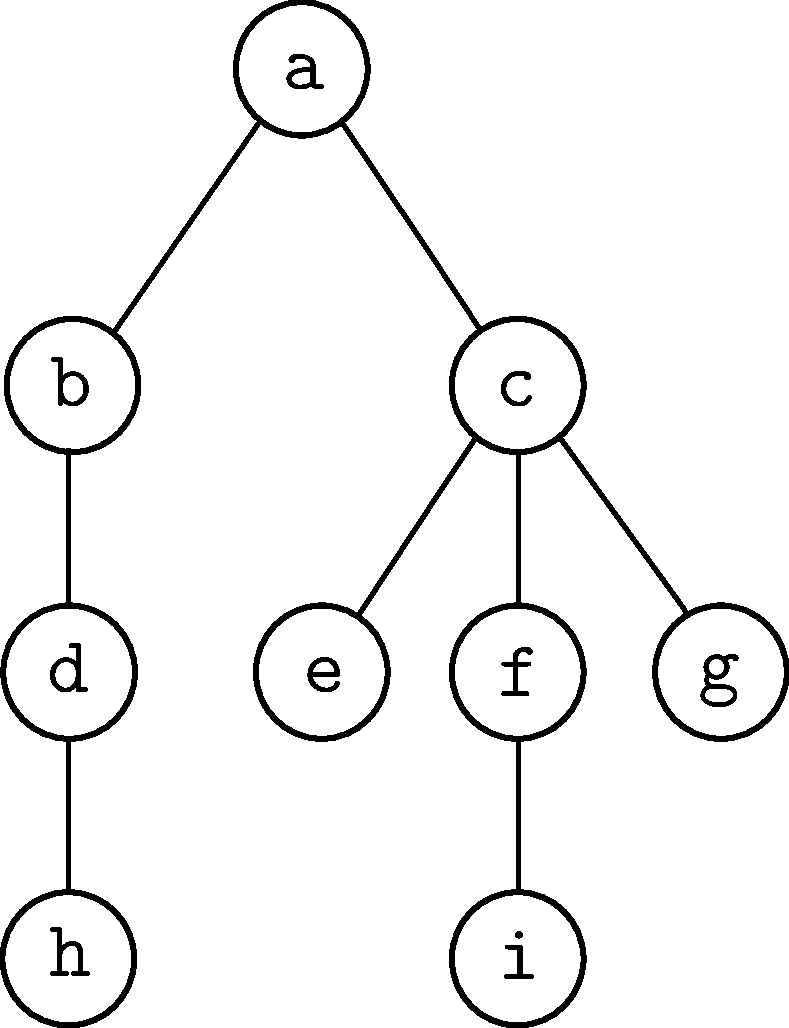
\includegraphics[width=0.25\textwidth]{two-trees-1.pdf}}
  \hspace{0.1\textwidth}
  \subfigure[\texttt{t2}]{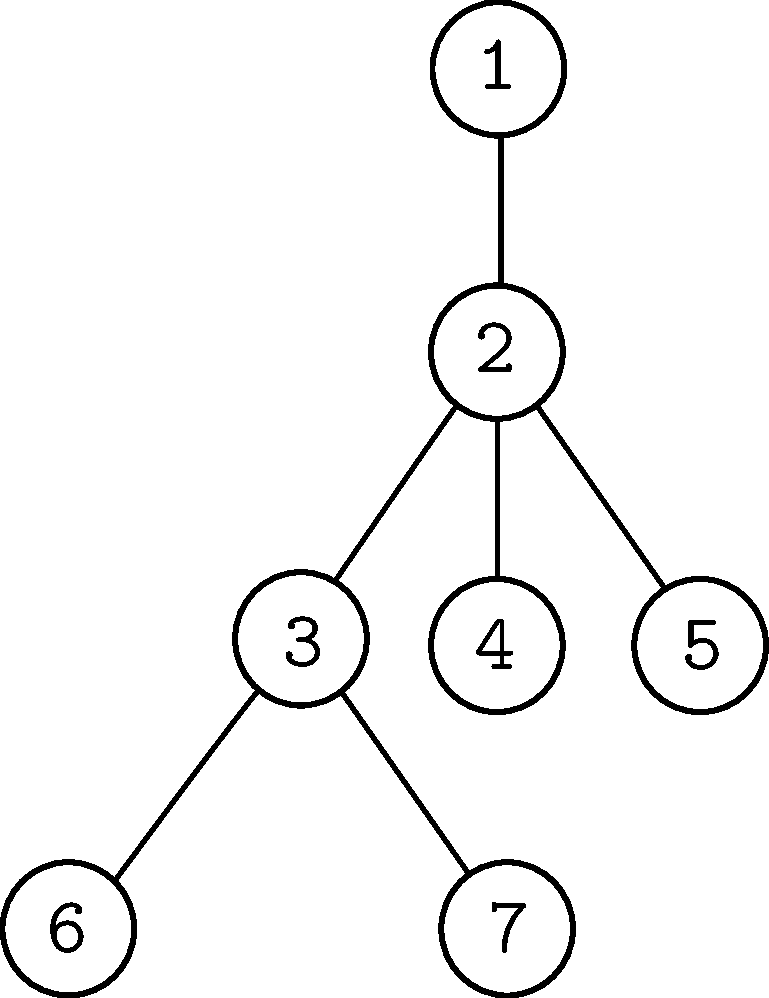
\includegraphics[width=0.25\textwidth]{two-trees-2.pdf}}
  \caption{两棵树}
  \label{fig:two_trees}
\end{figure}

树可以用嵌套列表来表示\index{lists!as trees}。第~\pageref{sec:function:recursion_on_subtrees}
页上描述了一种将一类树表示成列表的方法。这里我们采用另一种方法,允许内
部节点带有~(原子的) 值,以及任意数量的孩子。在这种表示方法里,内部节点
变成了一个列表;其~car 包含保存在这个节点上的值,其~cdr 包含该节点孩子
的表示。例如,图~\ref{fig:two_trees} 里显示的两棵树可以被表示成:
\begin{lstlisting}
(define t1 '(a (b (d h)) (c e (f i) g)))
(define t2 '(1 (2 (3 6 7) 4 5)))
\end{lstlisting}

\begin{figure}
\begin{lstlisting}
(define (dft tree)
  (cond ((null? tree) ())
        ((not (pair? tree)) (write tree))
        (else (dft (car tree))
              (dft (cdr tree)))))

(define *saved* ())

(define (dft-node tree)
  (cond ((null? tree) (restart))
        ((not (pair? tree)) tree)
        (else (call-with-current-continuation
                (lambda (cc)
                  (set! *saved*
                        (cons (lambda ()
                                (cc (dft-node (cdr tree))))
                              *saved*))
                  (dft-node (car tree)))))))

(define (restart)
  (if (null? *saved*)
      'done
      (let ((cont (car *saved*)))
        (set! *saved* (cdr *saved*))
        (cont))))

(define (dft2 tree)
  (set! *saved* ())
  (let ((node (dft-node tree)))
    (cond ((eq? node 'done) ())
          (else (write node)
                (restart)))))
\end{lstlisting}
  \caption{用\continuation{}来遍历树}
  \label{fig:tree_traversal_using_continuations}
  \index{stacks 栈!use for iteration}
\end{figure}

图~\ref{fig:tree_traversal_using_continuations} 中的函数能在这样的树上做深
度优先搜索。在实际的程序里,我们可能想要在遇到节点时用它们做一些事。
这里只是打印它们。为了便于比较,这里给出的函数~\texttt{dft} 
实现了通常的深度优先遍历:
\begin{lstlisting}
> (dft t1)
ABDHCEFIG()
\end{lstlisting}
函数~\texttt{dft-node} 按照同样的路径遍历这棵树,但每次只处理一个节点。
当~\texttt{dft-node} 到达一个节点时,它跟着节点的~car 走,并且
在~\texttt{*saved*} 里压入一个\continuation{}来浏览其~cdr 部分。
\begin{lstlisting}
> (dft-node t1)
A
\end{lstlisting}
调用~\texttt{restart} 可以继续遍历,作法是弹出最近保存的
\continuation{}并调用它。
\begin{lstlisting}
> (restart)
B
\end{lstlisting}
最后,所有之前保存的状态都用完了,\texttt{restart} 通过返回~\texttt{done}
来通告这一事实:
\begin{lstlisting}
$\vdots$
> (restart)
G
> (restart)
DONE
\end{lstlisting}

最后,函数~\texttt{dft2} 把我们刚刚手工完成的工作干净漂亮地一笔带过:
\begin{lstlisting}
> (dft2 t1)
ABDHCEFIG()
\end{lstlisting}
注意到在~\texttt{dft2} 的定义里没有显式的递归或迭代\index{iteration!without loops}:后继的节点被打印
出来,是因为由~\texttt{restart} 引入的\continuation{}总是返回
到~\texttt{dft-node} 中同样的~\texttt{cond} 子句那里。

这种程序的工作方式就跟采矿\index{mines 采矿}差不多。它先调用~\texttt{dft-node} 初步挖出一
个矿坑。一旦返回值不是~\texttt{done},\texttt{dft-node} 后面的代码
将调用~\texttt{restart} 将控制权发回到栈上。这个过程会一直持续,直到到返回值表明矿
被采空。这时,\texttt{dft2} 将不再打印返回值,而是返回~\verb|#f|。
使用\continuation{}的搜索方式带来了一种编写程序的新思路:将合适
的代码放在栈上,然后不断地返回到那里来获得结果。

如果我们只是想同时遍历一棵树,就像~\texttt{dft2} 里那样,那么实在没
有必要使用这种技术。\texttt{dft-node} 的优势在于,可以同时运行它的多个
实例。假设有\emph{两}棵树,并且我们想要以深度优先的顺序生成其中
元素的叉积\index{trees 树!cross-products of 叉积}。
\begin{lstlisting}
> (set! *saved* ())
()
> (let ((node1 (dft-node t1)))
    (if (eq? node1 'done)
        'done
        (list node1 (dft-node t2))))
(A 1)
> (restart)
(A 2)
$\vdots$
> (restart)
(B 1)
$\vdots$
\end{lstlisting}
借助常规技术,我们必须采取显式的措施来保存我们在两棵树中的位置。而通
过\continuation{},则能非常自然地维护两个正在进行的遍历操作的状态。对于诸如本例的
简单情形,要保存我们在树中的位置还不算太难。树是持久性的数据结构,所以我
们至少有办法找到~``我们在树中的位置''。\continuation{}的过人之处在于,
即使没有持久性的数据结构与之关联,它同样可以在\emph{任何}的计算过程中轻松保存我们的位置。
这一计算甚至也不需要具有有限数量的状态,只要重启它们有限次就行了。

正如第~\ref{chap:prolog} 章将要展示的,这两种考虑被证实在~Prolog 的
实现中至关重要。在~Prolog 程序里,“搜索树”\index{search trees}并非真正的数据结构,而
只是程序生成结果的一种隐式方式。而且这些树经常是无穷大的,这种情况下,我
们不能指望在搜索下一棵树之前把整棵树都搜完,所以只得想个办法保存我们的位置,
除此之外别无选择。

\section{\continuation{}传递宏}
\label{sec:continuation-passing_macros}
\index{continuation-passing macros}

虽然~Common Lisp 没有提供~\texttt{call/cc},但是再加把劲,我们就可以
像在~Scheme 里那样做到同样的事情了。本节展示如何用宏在~Common Lisp 程序
中构造\continuation{}。Scheme 的\continuation{}给了我们两样东西:
\begin{enumerate}
\item \continuation{}被创建时所有变量的绑定。
\item 计算的状态\pozhehao{}从那时起将要发生什么。
\end{enumerate}
在一个词法作用域的~Lisp 里,闭包给了我们前者。可以看出我
们也能使用闭包来获得后者,办法是把计算的状态同样也保存在变量绑定里。

%% Figure 20.4: change global value of *cont* according to errata
\begin{figure}
\begin{lstlisting}
(defvar *actual-cont* #'values)

(define-symbol-macro *cont*
  *actual-cont*)

(defmacro =lambda (parms &body body)
  `#'(lambda (*cont* ,@parms) ,@body))

(defmacro =defun (name parms &body body)
  (let ((f (intern (concatenate 'string
                                "=" (symbol-name name)))))
    `(progn
       (defmacro ,name ,parms
         `(,',f *cont* ,,@parms))
       (defun ,f (*cont* ,@parms) ,@body))))

(defmacro =bind (parms expr &body body)
  `(let ((*cont* #'(lambda ,parms ,@body))) ,expr))

(defmacro =values (&rest retvals)
  `(funcall *cont* ,@retvals))

(defmacro =funcall (fn &rest args)
  `(funcall ,fn *cont* ,@args))

(defmacro =apply (fn &rest args)
  `(apply ,fn *cont* ,@args))
\end{lstlisting}
  \caption{\continuation{}传递宏}
  \label{fig:continuation-passing_macros}
  \index{lambda@\texttt{=lambda}}
  \index{defun@\texttt{=defun}}
  \index{bind@\texttt{=bind}}
  \index{values@\texttt{=values}}
  \index{funcall@\texttt{=funcall}}
  \index{apply@\texttt{=apply}}
\end{figure}

图~\ref{fig:continuation-passing_macros} 给出的宏让我们能在保
留\continuation{}的情况下,进行函数调用。\index{functions 函数!combined with macros}这些宏取代了几个内置的~Common
Lisp form,它们被用来定义函数,进行函数调用,以及返回函数值。

如果有函数需要使用\continuation{},或者这个函数所调用的函数要用到\continuation{},那么该函数
就该用~\texttt{=defun} 而不是~\texttt{defun} 定义\note{266}。
\texttt{=defun} 的语法和~\texttt{defun} 相同,但其效果有些微妙的差别。
\texttt{=defun} 定义的并不是单单一个函数,它实际上定义了一个函数和一个宏,这个宏会展开
成对该函数的调用\index{macros 宏!macro-defining}\index{macros 宏!combined with functions}。
(宏定义必须在先\index{macros 宏!position in source code},原因是被定义的函数有可能会调用自己。)
函数的主体就是传给~\texttt{=defun} 的那个,但还另有一个形参,
即~\verb|*cont*|\index{*cont*@\texttt{*cont*}},它被连接在原有的形参列表上。在宏展开式里,\texttt{*cont*} 会和其他参数一同传给
这个函数。所以
\begin{lstlisting}
(=defun add1 (x) (=values (1+ x)))
\end{lstlisting}
宏展开成
\begin{lstlisting}
(progn (defmacro add1 (x)
         `(=add1 *cont* ,x))
       (defun =add1 (*cont* x)
         (=values (1+ x))))
\end{lstlisting}

当调用~\texttt{add1} 时,实际被调用的不是函数而是个宏。这个宏
会展开成一个函数调用%
\footnote{由~\texttt{=defun} 产生的函数被有意地赋予了~intern\index{intern@\texttt{intern}} 了的名字,好让这些函数能够被~
  \texttt{trace}\index{trace@\texttt{trace}}。如果没有必要做~trace 的话,用 gensym 来作为它们的名字应该会更安全些。}\label{trace}%
,但是另外带了一个参数:\texttt{*cont*}。所以,在调用~\texttt{=defun} 定义的操作符的时候,
\texttt{*cont*} 的当前值总是被默默地传递着。

那~\texttt{*cont*} 有什么用呢?它将被绑定到当前的\continuation{}。
\texttt{=values} 的定义显示了这个\continuation{}的用场。只要是用
~\texttt{=defun} 定义的函数,都必须通过~\texttt{=values} 来返回值,或者
调用另一个使用~\verb|=values| 的函数。\texttt{=values} 的语法与~Common Lisp
的~\texttt{values} 相同。如果有个带有相同数量参数的~\texttt{=bind}\label{page:bind} 等着它的话,
它可以返回多值,但它不能返回多值到~toplevel。\note{267}

参数~\texttt{*cont*} 告诉那个由~\texttt{=defun} 定义的函数对其返回值做
什么。当~\texttt{=values} 被宏展开时,它将捕捉~\texttt{*cont*}\index{capture 捕捉!intentional},并用
它模拟从函数返回值的过程。表达式
\begin{lstlisting}
(=values (1+ n))
\end{lstlisting}
会展开成
\begin{lstlisting}
(funcall *cont* (1+ n))
\end{lstlisting}
在~toplevel 下,\texttt{*cont*} 的值是~\verb|#'values|\footnote{译
  者注:原文是~``\texttt{*cont*} 的值是~\texttt{identity}'',这是错误
  的。并且原书勘误修正了图~\ref{fig:continuation-passing_macros}
  中对应的~\texttt{*cont*} 定义,这里译文也随之做了修改。},
这就相当于一个真正的~\texttt{values} 多值返回。当我们在~toplevel
下调用~\texttt{(add1 2)} 时,这个调用的宏展开式与下式等价
\begin{lstlisting}
(funcall #'(lambda (*cont* n) (=values (1+ n))) *cont* 2)
\end{lstlisting}
\texttt{*cont*} 的引用在这种情况下将得到全局绑定。因而,\texttt{=values} 表
达式在宏展开后将等价于下式
\begin{lstlisting}
(funcall #'values (1+ n))
\end{lstlisting}
即把在~\texttt{n} 上加~\texttt{1},并返回结果。

在类似~\texttt{add1} 的函数里,我们克服了重重困难,不过是
为了模拟~Lisp 进行函数调用和返回值的过程:
\begin{lstlisting}
> (=defun bar (x)
    (=values (list 'a (add1 x))))
BAR
> (bar 5)
(A 6)
\end{lstlisting}
关键在于,现在有了``函数调用''和``函数返回''可供差遣,而且如果
愿意的话,我们还可以把它们用在其他地方。

我们之所以能获得\continuation{}的效果,要归功于对~\texttt{*cont*} 的操控。虽
然~\texttt{*cont*} 的值是全局的,但这个全局变量很少用到:
\texttt{*cont*} 几乎总是一个形参,它被~\texttt{=values} 以及
用~\texttt{=defun} 定义的宏所捕捉。例如在~\texttt{add1} 的函数体里,
\texttt{*cont*} 就是一个形参而非全局变量\index{variables 变量!global 全局}。这个区别是很重要的,因为如
果~\texttt{*cont*} 不是一个局部变量的话这些宏将无法工作。\footnote{译
  者注:原书中在这里还有一句话:``That's why \texttt{*cont*} is given
  its initial value in a \texttt{setq} instead of a \texttt{defvar}:
  the latter would also proclaim it to be \texttt{special}.'' 
  原作者假设~\texttt{*cont*} 全局变量是词法作用域的,但这违
  反了~Common Lisp 标准。为了能在现代~Common Lisp 实现上运行这些代码,
  译文采纳了~\href{http://www.cliki.net/On\%20Lisp}{\textsc{Cliki}} 上
  给出的一个解决方案,使用符号宏来模拟词法变量。具体参见
  图~\ref{fig:continuation-passing_macros} 中修改过的代码。}
图~\ref{fig:continuation-passing_macros} 中的第三个宏,\texttt{=bind},
其用法和~\texttt{multiple-value-bind} 相同。它接受一个参
数列表,一个表达式,以及一个代码体:参数将被绑定到表达式返回的值上,而
代码体在这些绑定下被求值。倘若一个由~\texttt{=defun} 定义的函数,
在被调用之后,需要对另一个表达式进行求值,那么就应该使用~\texttt{=bind} 宏。
\begin{lstlisting}
> (=defun message ()
    (=values 'hello 'there))
MESSAGE
> (=defun baz ()
    (=bind (m n) (message)
      (=values (list m n))))
BAZ
> (baz)
(HELLO THERE)
\end{lstlisting}
注意到~\texttt{=bind} 的展开式会创建一个称为~\texttt{*cont*} 的新
变量。\texttt{baz} 的主体展开成:
\begin{lstlisting}
(let ((*cont* #'(lambda (m n)
                  (=values (list m n)))))
  (message))
\end{lstlisting}
然后会变成:
\begin{lstlisting}
(let ((*cont* #'(lambda (m n)
                  (funcall *cont* (list m n)))))
  (=message *cont*))
\end{lstlisting}
由于~\texttt{*cont*} 的新值是~\texttt{=bind} 表达式的代码体,所以
当~\texttt{message} 通过函数调用~\texttt{*cont*} 来~``返回'' 时,结果
将是去求值这个代码体。尽管如此~(并且这里是关键),在~\texttt{=bind} 的
主体里:
\begin{lstlisting}
#'(lambda (m n)
    (funcall *cont* (list m n)))
\end{lstlisting}
作为参数传递给~\texttt{=baz} 的~\texttt{*cont*} 仍然是可见的,所以当代
码的主体求值到一个~\texttt{=values} 时,\emph{它}将能够返回到最初的
主调函数那里。所有闭包环环相扣:每个~\texttt{*cont*} 的绑定
都包含了上一个~\texttt{*cont*} 绑定的闭包,它们串成一条锁链\index{chains of closures},锁链的尽头指向
那个全局的值。

在这里,我们也可以观察到更小规模的同样现象:
\begin{lstlisting}
> (let ((f #'values))
    (let ((g #'(lambda (x) (funcall f (list 'a x)))))
      #'(lambda (x) (funcall g (list 'b x)))))
#<Interpreted-Function BF6326>
> (funcall * 2)
(A (B 2))
\end{lstlisting}
本例创建了一个函数,它是含有指向~\texttt{g} 的引用的闭包,
而~\texttt{g} 本身也是一个含有到~\texttt{f} 的引用的闭包。第~\pageref{fig:compilation_with_static_reference} 页上的网络编
译器中曾构造过类似的闭包链。

剩下两个宏,分别是~\texttt{=apply} 和~\texttt{=funcall},它们适用于
由~\texttt{=lambda} 定义的函数。注意那些用~\texttt{=defun} 定义出来
的~``函数'',因为它们的真实身份是宏,所以不能作为参数传给~\texttt{apply}
或~\texttt{funcall}。解决这个问题的方法类似于第~\pageref{the_cons_4}
页上提到的技巧。也就是把调用包装在另一个~\texttt{=lambda} 里面:
\begin{lstlisting}
> (=defun add1 (x)
    (=values (1+ x)))
ADD1
> (let ((fn (=lambda (n) (add1 n))))
    (=bind (y) (=funcall fn 9)
      (format nil "9 + 1 = ~A" y)))
"9 + 1 = 10"
\end{lstlisting}

\begin{figure}
  \begin{enumerate}
  \item 一个用~\texttt{=defun} 定义的函数的参数列表必须完全由参数名组
    成。
  \item 使用\continuation{},或者调用其他做这件事的函数的函数,必须
    用~\texttt{=lambda} 或~\texttt{=defun} 来定义。
  \item 这些函数必须终结于用~\texttt{=values} 来返回值,或者调用其他遵守
    该约束的函数。
  \item\label{itm:tail-call} 如果一个~\texttt{=bind},\texttt{=values},或
    者~\texttt{=funcall} 表达式出现在一段代码里,它必须是一个尾调用。
    任何在~\texttt{=bind} 之后求值的代码必须放在其代码体里。所以如果我
    们想要依次有几个~\texttt{=bind},它们必须被嵌套:
\begin{lstlisting}
(=defun foo (x)
  (=bind (y) (bar x)
    (format t "Ho ")
    (=bind (z) (baz x)
      (format t "Hum.")
      (=values x y z))))
\end{lstlisting}
  \end{enumerate}
  \caption{\continuation{}传递宏的限制}
  \label{fig:restrictions_on_continuation-passing_macros}
  \index{continuation-passing macros!restrictions on}
\end{figure}

图~\ref{fig:restrictions_on_continuation-passing_macros} 总结了所有因
\continuation{}传递宏而引入的限制。如果有函数既不保存\continuation{},也不调用其他保存\continuation{}的函数,
那它就没有必要使用这些特殊的宏。比如像~\texttt{list} 这样的内置函数就没有这个需要。

\begin{figure}
\begin{lstlisting}
(defun dft (tree)
  (cond ((null tree) nil)
        ((atom tree) (princ tree))
        (t (dft (car tree))
           (dft (cdr tree)))))

(defvar *saved* nil)

(=defun re-start ()
  (if *saved*
      (funcall (pop *saved*))
      (=values 'done)))

(=defun dft-node (tree)
  (cond ((null tree) (re-start))
        ((atom tree) (=values tree))
        (t (push #'(lambda () (dft-node (cdr tree)))
                  *saved*)
                 (dft-node (car tree)))))

(=defun dft2 (tree)
  (setq *saved* nil)
  (=bind (node) (dft-node tree)
    (cond ((eq node 'done) (=values nil))
          (t (princ node)
             (re-start)))))
\end{lstlisting}
  \caption{使用\continuation{}传递宏的树遍历}
  \label{fig:tree_traversal_using_continuation-passing_macros}
\end{figure}

图~\ref{fig:tree_traversal_using_continuation-passing_macros} 中把来自
图~\ref{fig:tree_traversal_using_continuations} 的代码\footnote{译者
  注:这段代码与原书有一些出入:首先~\texttt{(setq *saved* nil)} 被
  改为~\texttt{(defvar *saved* nil)};其次
  将~\texttt{restart} 改为~\texttt{re-start} 以避免和~Common Lisp 已
  有的符号冲突,并且将~\texttt{re-start} 的定义放在~\texttt{dft-node}
  的定义之前以确保后者在编译时可以找到~\texttt{re-start} 的定义。}
从~Scheme 翻译成了~Common Lisp,并且用\continuation{}传递宏代替了~Scheme
\continuation{}。以同一棵树为例,\texttt{dft2} 和之前一样工作正常:
\begin{lstlisting}
> (setq t1 '(a (b (d h)) (c e (f i) g))
        t2 '(1 (2 (3 6 7) 4 5)))
(1 (2 (3 6 7) 4 5))
> (dft2 t1)
ABDHCEFIG
NIL
\end{lstlisting}

和~Scheme 里一样,我们仍然可以保存多路遍历的状态,尽管这个例子会显得有些冗长:
\begin{lstlisting}
> (=bind (node1) (dft-node t1)
    (if (eq node1 'done)
        'done
        (=bind (node2) (dft-node t2)
          (list node1 node2))))
(A 1)
> (re-start)
(A 2)
$\vdots$
> (re-start)
(B 1)
$\vdots$
\end{lstlisting}
通过把词法闭包编结成串,Common Lisp 程序得以构造自己的
\continuation{}。幸运的是,这些闭包是由
图~\ref{fig:continuation-passing_macros} 中血汗工厂给出的宏编织而成的,
用户可以不用关心它们的出处,而直接享用劳动成果。

第~\ref{chap:multiple_processes}--\ref{chap:prolog} 章都以某种方式依赖
于\continuation{}。这些章节将显示\continuation{}是一种能力非凡的抽象。
它可能不会很快,如果是在语言层面之上,用宏实现的话,其性能可能会更会
大打折扣。但是,我们基于\continuation{}构造的抽象层可以大大加快某些程序的编写
速度,而且提高编程效率也有着其实际意义。

\section{Code-Walker 和~CPS Conversion}
\label{sec:code-walkers_and_cps_conversion}

从前一节里描述的宏,我们看到了一种折衷。只有用特定的方式编写程序,
我们才能施展\continuation{}的威力。
图~\ref{fig:restrictions_on_continuation-passing_macros} 的第~\ref{itm:tail-call} 条规则
意味着我们必须把代码写成
\begin{lstlisting}
(=bind (x) (fn y)
  (list 'a x))
\end{lstlisting}
而不能是
\begin{lstlisting}[escapechar=\@]
(list 'a@\hfill@; wrong
      (=bind (x) (fn y) x))
\end{lstlisting}
真正的~\verb|call/cc| 就不会把这种限制强加于程序员。
\texttt{call/cc} 可以捕捉到所有程序中任意地方的
\continuation{}。尽管我们也能实现具有~\texttt{call/cc} 所有功能的操作符,
但那还要做很多工作。本节会大略提一下,如果真要这样做的话,还有哪些事有待完成。

Lisp 程序可以转换成一种称为~``continuation-passing style'' (\continuation{}传递风格) 的形式。
经过完全的~\textsc{cps}\index{continuation-passing style (CPS)@continuation-passing (\textsc{cps})} 转换的程序是不可读的,但我们可以通过观察被部分转换了的代码来体会这个过程的思想。下面这个用于求逆列表的函数\note{273-1}:
\begin{lstlisting}
(defun rev (x)
  (if (null x)
      nil
      (append (rev (cdr x)) (list (car x)))))
\end{lstlisting}
产生的等价\continuation{}传递版本:
\begin{lstlisting}
(defun rev2 (x)
  (revc x #'identity))

(defun revc (x k)
  (if (null x)
      (funcall k nil)
      (revc (cdr x)
            #'(lambda (w)
                (funcall k (append w (list (car x))))))))
\end{lstlisting}

在~continuation-passing style 里,函数得到了一个附加的形参~(这里是~\texttt{k}),
其值将是当前的\continuation{}。这个\continuation{}是个闭包,它代表了对函数
的当前值应该做些什么。在第一次递归时,\continuation{}是~\texttt{identity};
此时函数的任务就是返回其当前的值。在第二次递归时,\continuation{}
将等价于
\begin{lstlisting}
#'(lambda (w)
    (identity (append w (list (car x)))))
\end{lstlisting}
也就是说要做的事就是追加一个列表的~car 到当前的值上,然后返回它。

一旦可以进行~\textsc{cps} 转换,实现~\texttt{call/cc} 就易如反掌了。
在带有~\textsc{cps} 转换的程序里,当前的整个\continuation{}总是存在
的,这样~\texttt{call/cc} 就可以实现成一个简单的宏,将一些函数作为一个
参数来和它一起调用就好了。

为了做~\textsc{cps} 转换,我们需要~\emph{code-walker}\label{expl:code-walker}\index{code-walkers},
它是一种能够遍历程序源代码树的程序。为~Common Lisp 编写~code-walker 并非易事。
\note{273-2}
要真正能有用,code-walker 的功能不能仅限于简单地遍历表达式。它
还需要相当了解表达式的作用。例如,code-walker 不能只是在符号
的层面上思考。比如,符号至少可以代表,它本身,一个函数,变量,代码块
名称,或是一个~\texttt{go} 标签。code-walker 必须根据上下文,
分辨出符号的种类,并进行相应的操作。

由于编写~code-walker 超出了本书的范围,所以本章里描述的宏只是最现实
的替代品。本章中的宏将用户跟构建\continuation{}的工作分离开了。如果有用
户编写了相当接近于~\textsc{cps} 的程序,这些宏可以做其余的事情。第~\ref{itm:tail-call}
条规则实际上说的是:如果紧接着~\texttt{=bind} 表达式的每样东西都在其代
码体里,那么在~\texttt{*cont*} 的值和~\texttt{=bind} 主体中的代码之间,
程序有足够的信息用来构造当前的\continuation{}。

\texttt{=bind} 宏故意写成这样以使得这种编程风格看起来自然些。在实践中
由\continuation{}传递宏所引入的各种限制还是可以容忍的。

%%% Local Variables:
%%% coding: utf-8
%%% mode: latex
%%% TeX-master: "onlisp-cn"
%%% End:

%!TEX encoding = UTF-8 Unicode
% $Id: 21-multiple_processes.tex 17 2014-03-09 13:05:41Z binghe $

\chapter{多进程}
\label{chap:multiple_processes}

上一章展示了\continuation{}是如何使运行中的程序获知自己的状态,并且把它保存起来
以便之后重新执行的。这一章将讨论一种计算模型,在这种模型中,计算机运行的不是单个\emph{程序},
而是一组独立的\emph{进程}\index{processes 进程}。进程的概念和程序
状态这一概念相当接近。通过在前一章的宏的基础上再写一层宏,我们就可以把多进程的机
制\index{multiprocessing 多进程的机制}融入到~Common Lisp 程序中。

\section{进程抽象}
\label{sec:the_process_abstraction}

多进程这种表现形式,可以很方便地表示并行处理多个任务的程序。传统的处理器同时
只能执行一条指令。我们称多进程能同时处理多件事情,并不是说它通过某种方式克服了硬件的限
制,它真正的含义是:它使得我们可以在一个新的抽象层面上进行思考,在这个层面上我们不需
要明确地指定计算机在任何给定的时间在做什么。就像虚拟内存给我们制造了一个错觉,似乎
计算机的可用内存比它的物理内存还要大,同样的道理,多进程的概念使得我们可以假设计算
机可以一次运行多个程序。

从传统上说,对进程的研究属于操作系统领域的范畴。但进程抽象带来的进步并不局限于操
作系统。它们在其他实时的应用程序和计算机仿真中一样能大展身手。

有很多对于多进程的研究,它们的目的都是为了避免出现某些特定类型的问题。死锁是多进
程的一个经典问题:两个进程同时停下等待另一个做某些事情,就像两个人都拒绝在另一个
人之前跨过门槛。另一个问题是查询有可能碰到系统中数据不一致的状态\pozhehao{}例如,
一个余额查询正好在系统将资金从一个账户转移到另一个账户时发生。这一章只讨论进程抽
象本身;这里展示的代码可以用来测试避免死锁和不一致状态的算法,但代码本身没有对
这些问题提供任何保护。

%% 在本质上来说~(??In spirit)
这一章中的实现遵循了本书所有程序默默恪守的一条准则:尽可能少的扰乱~Lisp。在本质
上来说,程序应该尽可能多的让自己像是对语言的修改,而不是用语言写就的一个独立的应用程序
。使程序与~Lisp 协调一致可以使得程序更为健壮,好比部件配合良好的机器。这样做
也能事半功倍;有时你可以让~Lisp 为你代劳数量惊人的工作。

这一章的目标是构建一个支持多进程的的语言。我们的策略是通过添加一些操作符,将~Lisp 
变成这样的语言。我们语言的基本构成元素如下:

\begin{quote}
    \emph{函数} 由前一章的~\texttt{=defun} 或者~\texttt{=lambda} 宏定义。

    %% xxx 实例化~(??instantiate)
    \emph{进程} 由函数调用实例化。活动进程的数量和一个函数能够
    实例化的进程数量都没有限制。每个进程有一个优先级,初始值由创建时给出的参数指
    定。

    \emph{等待表达式~(Wait expressions)} 等待表达式接受一个变量,一个测试表达
    式和一段代码体。如果进程遇到等待表达式,进程将在这一点被挂起,直到测试表达式
    返回真。一旦进程重新开始执行,代码体会被求值,变量则被绑定到测试表达式的值。
    测试表达式通常不应该有副作用,因为它被求值的时间和频率没有任何保证。

    \emph{调度} 通过优先级来完成。在所有能够重新开始执行的进程中,系统会运行优
    先级最高的进程。

    \emph{默认进程} 在其他进程都不能执行时运行。它是一个~read-eval-print 循环
    。
    
    \emph{创建和删除} 绝大多数对象的操作可以即时进行。正在运行中的进
    程可以定义新的函数,实例化或者杀死进程。
\end{quote}

\continuation{}使得保存~Lisp 程序的状态成为可能。能够同时保存多个状态离实现多进程
也不太远了。有了前一章定义的宏做基础,我们只要不到~60 行的代码就可以实现多进程
。

\section{实现}

\begin{figure}
\begin{lstlisting}
(defstruct proc pri state wait)

(proclaim '(special *procs* *proc*))

(defvar *halt* (gensym))

(defvar *default-proc*
  (make-proc :state #'(lambda (x)
			(format t "~%>> ")
			(princ (eval (read)))
			(pick-process))))

(defmacro fork (expr pri)
  `(prog1 ',expr
     (push (make-proc
	    :state #'(lambda (,(gensym))
		       ,expr
		       (pick-process))
	    :pri ,pri)
	   *procs*)))

(defmacro program (name args &body body)
  `(=defun ,name ,args
	   (setq *procs* nil)
	   ,@body
	   (catch *halt* (loop (pick-process)))))
\end{lstlisting}
    \caption{进程结构及实例化}
    \label{fig:process_structure_and_instantiation}
\end{figure}

图~\ref{fig:process_structure_and_instantiation} 和图
~\ref{fig:process_scheduling} 包含了所有用来支持多进程的代码。图
~\ref{fig:process_structure_and_instantiation} 包含了基本数据结构、默认进程、初
始化、进程实例化的代码。进程,或者说~\texttt{proc}s,具有如下结构:

\begin{description}
  \item[\texttt{pri}] 进程的优先级,它应该是一个正数。

  \item[\texttt{state}] 是一个\continuation{},它用来表示一个挂起进程的状态
      \index{processes 进程!state of 的状态}。我们可以~funcall 一个进程的
      ~\texttt{state} 来重新启动它,

  \item[\texttt{wait}] 通常是一个函数,如果要让进程重新执行,它必须返回真,但
    刚创建的进程的~\texttt{wait} 为~\texttt{nil}。\texttt{wait}~为空
    的进程总是可以被重新执行。
\end{description}

程序使用三个全局变量:\texttt{*procs*},当前被挂起的进程列表;\texttt{*proc*},
正在运行的进程;还有~\texttt{*default-proc*},默认进程。

默认进程仅当没有其他进程可以运行时才会运行。它模拟~Lisp 的~toplevel 循环。在这个循环
中,用户可以终止程序,或者输入让挂起进程恢复执行的表达式。请注意,默认进程显式地调
用了~\texttt{eval}\index{eval@\texttt{eval}!explicit}。这是少数几个合理使用~\texttt{eval} 的情形之一。一般来说,我们不
赞成在运行时调用~\texttt{eval}\label{why-eval-is-bad},这有两个原因:\label{expl:eval}
\begin{enumerate}
    \item 效率低下:\texttt{eval}~直接处理原始列表,要么当场进行编译,要么在解释
        器中进行求值。不管哪种方式都比先编译再调用来得慢。
    \item 功能不够强大,因为表达式不在词法上下文中进行求值。举个例子,这就
        意味着你不能引用在被求值表达式之外可见的普通变量。
\end{enumerate}
\label{bad-eval}
通常来说,显式调用~\texttt{eval} 就像在机场礼品店\index{gift-shops, airport}买东西一样。已经是最后关头,你
只得高价购买选择有限的劣质商品。

像本例这样两条理由都不适用的情况是很少见的。我们没法提前将表达式编译好。直到读取
它们的时候才知道表达式是什么,所以没法事先知道。同样的,表达式无法引用它周遭的词
法环境,因为在~toplevel 输入的表达式处于空的词法环境\index{environment!null 空}中。事实上,这个函数的定义直
接反映了它的英语描述:它读取并求值用户的输入\footnote{译者注:即~\texttt{(eval
(read))}。}。

宏~\texttt{fork} 使用一个函数调用来实例化进程\index{processes 进程!instantiation
实例化}。函数像平时一样由~\texttt{=defun} 定义:

\begin{lstlisting}
(=defun foo (x)
  (format t "Foo was called with ~A.~%" x)
  (=values (1+ x)))
\end{lstlisting}

现在当我们以一个函数调用和优先级数值作为参数调用~fork 时:

\begin{lstlisting}
(fork (foo 2) 25)
\end{lstlisting}
一个新进程被加入到了~\texttt{*procs*} 里面。新进程的优先级为~25,
因为它还没有执行,所以~\texttt{proc-wait} 为~\texttt{nil},而
~\texttt{proc-state} 包含了以~\texttt{2} 为参数的对~\texttt{foo} 的调用。

宏~\texttt{program} 使我们可以创建一组进程并一起执行它们。下面的定义:

\begin{lstlisting}
(program two-foos (a b)
  (fork (foo a) 99)
  (fork (foo b) 99))
\end{lstlisting}
宏展开成了两个~\texttt{fork} 表达式,被夹在负责清除挂起进程的代码,以及不断选择
进程来运行的代码中间。%
% xxx Outside this loop, the macro establishes a tag to which control can
% be thrown to end the program. 知道意思,但不知道怎么说好
在这个循环外面,\texttt{program} 宏设置了一个~tag,把控制流抛~(throw) 到这
个~tag 的话,就会终止这个程序~(program)\footnote{译者
  注:\texttt{catch} 操作符的用法可见~\emph{CLHS} 中
  的~\href{http://www.lisp.org/HyperSpec/Body/speope_catch.html}{Special
    Operator CATCH} 一节。}。因为这个~tag 是个\gensym,所以它不会与用户
设置的~tag 冲突。定义成~\texttt{program}的一组进程不返回任何值,而且它
们只应该在~toplevel 被调用。

\begin{figure}
\begin{lstlisting}
(defun pick-process ()
  (multiple-value-bind (p val) (most-urgent-process)
    (setq *proc* p
	  *procs* (delete p *procs*))
    (funcall (proc-state p) val)))

(defun most-urgent-process ()
  (let ((proc1 *default-proc*) (max -1) (val1 t))
    (dolist (p *procs*)
      (let ((pri (proc-pri p)))
	(if (> pri max)
	    (let ((val (or (not (proc-wait p))
			   (funcall (proc-wait p)))))
	      (when val
		(setq proc1 p
		      max pri
		      val1 val))))))
    (values proc1 val1)))

(defun arbitrator (test cont)
  (setf (proc-state *proc*) cont
	(proc-wait *proc*) test)
  (push *proc* *procs*)
  (pick-process))

(defmacro wait (parm test &body body)
  `(arbitrator #'(lambda () ,test)
	       #'(lambda (,parm) ,@body)))

(defmacro yield (&body body)
  `(arbitrator nil #'(lambda (,(gensym)) ,@body)))

(defun setpri (n) (setf (proc-pri *proc*) n))

(defun halt (&optional val) (throw *halt* val))

(defun kill (&optional obj &rest args)
  (if obj
      (setq *procs* (apply #'delete obj *procs* args))
      (pick-process)))
\end{lstlisting}
    \caption{进程调度}
    \label{fig:process_scheduling}
    \index{wait@\texttt{wait}}
\end{figure}

进程实例化之后,进程调度\index{processes 进程!scheduling 调度}代码开始执行。它的
代码见图~\ref{fig:process_scheduling}。函数~\texttt{pick-process} 在可以继续执行
的进程中,选出优先级最高的一个,然后运行它。把这个进程找出来是
~\texttt{most-urgent-process} 的工作。如果一个挂起的进程没有~\texttt{wait} 函数
或者它的~\texttt{wait} 函数返回真,那么它就被允许运行。在所有被允许运行的进程中,具有
最高优先级的被选中。胜出的进程和它的~\texttt{wait} 函数~(如果有的话)返回的值被返
回给~\texttt{pick-process}。获胜进程总是存在,因为默认进程总是想要执行。

\begin{figure}
\begin{lstlisting}
(defvar *open-doors* nil)

(=defun pedestrian ()
  (wait d (car *open-doors*)
    (format t "Entering ~A~%" d)))

(program ped ()	 
  (fork (pedestrian) 1))
\end{lstlisting}
\caption{有一个等待的进程}
\label{fig:one_process_with_one_wait}
\end{figure}

图~\ref{fig:process_scheduling} 中其余的代码定义了用于在进程间切换控制权的操作符
。标准的等待表达式是~\texttt{wait},就像图~\ref{fig:one_process_with_one_wait}~
中函数~\texttt{pedestrian} 使用的那样。在这个例子中,进程一直等到列表
~\texttt{*open-doors*} 中有东西为止,然后打印一条消息:

\begin{lstlisting}
> (ped)
>> (push 'door2 *open-doors*)
Entering DOOR2
>> (halt)
NIL
\end{lstlisting}

一个~\texttt{wait} 在实质上来说与~\texttt{=bind}~(第~\pageref{page:bind} 页) 相
似,而且有着一样的限制,那就是它必须在最后被求值。任何我们希望在~\texttt{wait} 之
后执行的东西必须被放在它的代码体中。因此如果我们想要让一个进程等待多次,那等待表%
% xxx By asserting facts aimed at one another
达式必须被嵌套。通过声明互相针对的事实,进程可以相互配合以达到某个目标,就像
在图~\ref{fig:synchronization_with_a_blackboard} 中一样。

\begin{figure}
\begin{lstlisting}
(defvar *bboard* nil)

(defun claim (&rest f) (push f *bboard*))

(defun unclaim (&rest f) (pull f *bboard* :test #'equal))

(defun check (&rest f) (find f *bboard* :test #'equal))

(=defun visitor (door)
  (format t "Approach ~A. " door)
  (claim 'knock door)
  (wait d (check 'open door)
    (format t "Enter ~A. " door)
    (unclaim 'knock door)
    (claim 'inside door)))

(=defun host (door)
  (wait k (check 'knock door)
    (format t "Open ~A. " door)
    (claim 'open door)
    (wait g (check 'inside door)
      (format t "Close ~A.~%" door)
      (unclaim 'open door))))

(program ballet ()
  (fork (visitor 'door1) 1)
  (fork (host 'door1) 1)
  (fork (visitor 'door2) 1)
  (fork (host 'door2) 1))
\end{lstlisting}
\caption{利用黑板进行同步}
\label{fig:synchronization_with_a_blackboard}
\end{figure}

如果被给予相同的~\texttt{door},从~\texttt{visitor} 和~\texttt{host} 实例化的进
程会通过黑板\index{blackboards 黑板}上的消息互相交换控制权:

\begin{lstlisting}
> (ballet)
Approach DOOR2. Open DOOR2. Enter DOOR2. Close DOOR2.
Approach DOOR1. Open DOOR1. Enter DOOR1. Close DOOR1.
>>
\end{lstlisting}

还有另外一类更简单的等待表达式:\texttt{yield},它的唯一目的是让其他更高优先级
的进程有机会运行。\texttt{setpri}~重置当前进程的优先级,一个进程可能在执行
~\texttt{setpri} 表达式后想要让出控制权。就像~\texttt{wait} 一样,在
~\texttt{yield} 之后执行的代码都必须被放在它的代码体中。

\begin{figure}
\begin{lstlisting}
(=defun capture (city)
  (take city)
  (setpri 1)
  (yield
    (fortify city)))

(=defun plunder (city)
  (loot city)
  (ransom city))

(defun take (c) (format t "Liberating ~A.~%" c))

(defun fortify (c) (format t "Rebuilding ~A.~%" c))

(defun loot (c) (format t "Nationalizing ~A.~%" c))

(defun ransom (c) (format t "Refinancing ~A.~%" c))

(program barbarians ()
  (fork (capture ’rome) 100)
  (fork (plunder ’rome) 98))
\end{lstlisting}
\caption{改变进程优先级的效果}
\label{fig:effect_of_changing_priorities}
\index{Rome 罗马}
\end{figure}

图~\ref{fig:effect_of_changing_priorities} 中的程序说明了这两个操作符如何相互工
作。开始时,野蛮人\index{barbarians 野蛮人}有两个目的:占领罗马和掠夺它。占领城
市有着~(稍微) 高一些的优先级,因此会先执行。然而,在城市沦陷之后,
\texttt{capture}~进程的优先级减小到~1。之后会有一次投票,而~\texttt{plunder},作
为最高优先级的进程开始运行。
\begin{lstlisting}
> (barbarians)
Liberating ROME.
Nationalizing ROME.
Refinancing ROME.
Rebuilding ROME.
>>
\end{lstlisting}
只有在蛮族掠夺了罗马的宫殿,并勒索了贵族之后,\verb|capture| 进程才会恢复执
行,此时他们开始为其领地建筑防御工事。

等待表达式的背后是一个更通用的~\texttt{arbitrator}。这个函数保存当前进程,然后调用
~\texttt{pick-process} 来再次执行某个进程~(有可能与当前进程为同一个)。它有
两个参数:一个测试函数和一个\continuation{}。前者会被存储为挂起进程的
~\texttt{proc-wait},在以后被调用来检查它是否可以被重新执行。

宏~\texttt{wait} 和~\texttt{yield} 通过简单的把它们的代码体包在~\lexpr{}中来建立这
个\continuation{}函数。例如:

\begin{lstlisting}
(wait d (car *bboard*) (=values d))
\end{lstlisting}
被展开成:
\begin{lstlisting}
(arbitrator #'(lambda () (car *bboard*))
            #'(lambda (d) (=values d)))
\end{lstlisting}
如果代码遵循了图~\ref{fig:restrictions_on_continuation-passing_macros} 列出的限
制,构造一个~\texttt{wait} 代码体的闭包就可以保存当前的整个\continuation{}\index{continuation-passing macros!use in multiprocessing}。随着它
的~\texttt{=values} 被展开,第二个参数变成:
\begin{lstlisting}
#'(lambda (d) (funcall *cont* d))
\end{lstlisting}
由于这个闭包中有一个指向~\texttt{*cont*} 的引用,被这个等待函数挂起的进
程将会拥有一个句柄~(handle),通过它,这个进程就能回到它当初被挂起的那一
刻。

\texttt{halt}~操作符通过将控制权抛回~\texttt{program} 展开式建立的标签终止整个进
程组\footnote{译者注:可以认为宏~\texttt{program} 建立的由一组同时执行的进程组成
的程序,但为与“程序”相区别,这里把~program 翻译成“进程组”。}。它接受一个可选参数
,该参数的值会被作为这个进程组的值返回。因为默认进程始终想要执行,所以终止整个程
序的唯一的方法是显式的调用~\texttt{halt}。\texttt{halt}~后面是什么代码并没有关系,
因为这些代码不会被求值。

单个进程可以通过调用~\texttt{kill} 来杀死。如果没有参数,这个操作符杀死当前进程
。这种情况下,\texttt{kill}~就像是一个不保存当前进程的等待表达式。如果
~\texttt{kill} 给定了参数,它们将成为进程列表上的~\texttt{delete} 操作的参数。在
现在的代码中,\texttt{kill} 表达式没有什么好说的,因为进程没有许多的属性来被引用
。然而,更复杂的系统会为它的进程附加更多的信息\pozhehao{}时间戳、拥有者等等。默
认进程不能被杀死,因为它并没有被保存在~\texttt{*procs*} 中。

\section{不那么快速的原型}
\index{rapid prototyping 快速原型开发}

通过\continuation{}模拟的进程,其性能远不及真实操作系统的进程。那么,这一
章中的程序又有什么用处呢?

这些程序的用处类似于草图\index{sketches 草图}。不管在\emph{探索式编程}\index{exploratory
  programming 探索式的编程}还是\emph{快速原型开发}中,这些程序其自身
并不是最终目的,更多的是作为实现人们想法的手段。在许多其他领域,为这个
目的服务的东西被称为草图。在理论上,建筑师可以在他的脑海里构思出整栋大
楼。但多数建筑师似乎在手里握着笔的时候能想得更周详一些:一栋大楼的设计
通常在一系列草图中成型。

% xxx Like an architect’s first sketches, software prototypes tend to be drawn
% with a few sweeping strokes.
快速原型开发就是给软件作草图。就像建筑师的第一张草图,软件原型往往
也会由草草几笔一挥而就。在最初把想法付诸实现的时候,开销和效率的问题根本就没有纳入考量。
结果是,在这一阶段得到的往往就是无法施工的设计图,或是低效得不可救
药的软件。但无论如何,草图依然有它的价值,因为
\begin{enumerate}
    \item 它们简明的传达了信息
    \item 它们提供了试验的机会
\end{enumerate}
像后续章节中的程序一样,这一章描述的程序还只是初步的设计。它仅用寥寥几笔就勾勒出
了多进程大略的模样。而且,尽管它可能因为不够高效,不能使用在产品软件中,但是它
对于在多进程的其他方面作一些尝试还是很有用的,比如用来进行调度算法方面的试验。

第~\ref{chap:nondeterminism}--\ref{chap:prolog} 章展示了其他使用\continuation{}的
例子。它们都不够高效而不能使用在产品级的软件中。因为~Lisp 和快速原型开发一同演化
,Lisp~包含了很多专为原型开发打造的特性:低效但是方便的功能如属性列表,关键字参
数;推而广之,列表也是这类特性之一。\continuation{}可以说属于这一类特性。它们保存
了程序通常所需要的更多的状态。所以我们基于\continuation{}的~Prolog 实现就是一个例
子,通过这个实现我们能很好地理解这门语言,但是它的实现方式却是低效的。

本书更多的关注使用~Lisp 可以建立的抽象而不是效率问题。重要的是要意识
到,Lisp~既是一个适合写产品软件的语言也是一个适合写原型的语言。如
果~Lisp 有着低效的名声\index{Lisp!slowness of 低效},那大部分是因为程序员止步于原型。用~Lisp 写出快
速的程序很容易。不幸的是,用它写出低效的程序\emph{更是}容易。最初版本
的~Lisp 程序可以像钻石一样:娇小玲珑,清澈透明,而又笨重昂贵。也许有很大的诱
惑使人们就让它保留原状。

在其他的语言中,一旦你大功告成,程序能够运行\index{finished programs},那时程序
的效率可能就已经可以接受了。如果你用指甲盖大小的瓷砖来铺地板,自然是不会浪费多少
的。习惯用这种原则来开发软件的人可能会发现,克服“程序能工作就完工”这样的思维有些
困难。“虽然用~Lisp 你轻而易举就能把程序写出来,”他可能会想,“但哥们,这
些程序跑得太慢了。”事实上,两种看法都有问题。你可以写出快速的程序,但你得为此付
出努力。从这角度上说,使用~Lisp 就像生活在一个富裕而非贫穷的国度\index{rich countries 富裕的国度}:似乎人们不得不通
过工作来保持身材是种不幸,但这肯定比为了活下去而工作,自然只得消瘦下来要好。

在使用抽象能力较差的语言的时候,你想方设法实现的是功能。而在用~Lisp 的
时候,你努力改进的则是程序的运行速度。幸运的是,提升速度更容易一些;大
多数程序只在少数几个关键的地方才会关心速度。

%%% Local Variables:
%%% coding: utf-8
%%% mode: latex
%%% TeX-master: "onlisp-cn"
%%% End:

%!TEX encoding = UTF-8 Unicode
% $Id: 22-nondeterminism.tex 18 2014-03-12 22:35:24Z binghe $

\chapter{非确定性}
\label{chap:nondeterminism}

程序设计语言让我们得以从烦冗的细节中脱身而出。Lisp 是一门优秀的语言,其原因
在于它本身就帮我们处理如此之多的细枝末节,同时程序员对复杂问题的容忍
是有限度的,而~Lisp 让程序员能从他们有限的耐受度中发掘出最大的潜力。

本章将会解说宏是怎么样帮助~Lisp 解决另一类重要的细节问题的:即,将非确
定性算法转换为确定性算法的问题。

本章共分为五个部分。第一部分阐述了什么是非确定性。第二部分介绍了非确定
性~\emph{choose} 和~\emph{fail} 的一个~Scheme 实现,这个实现使用
了续延。第三部分呈现
了~\emph{choose} 和~\emph{fail} 的~Common Lisp 实现,这个版本的实现
基于第~\ref{chap:continuations} 章提到的~continuation-passing 宏。第四
部分展示了如何在脱离~Prolog 的情况下,来理解~cut 操作符。最后一部分提出
了一些改进最初版本的非确定性操作符的建议。

在本章定义的非确定性选择\index{nondeterministic choice 非确定性选择}操作符,将会在第~\ref{chap:parsing_with_atns}
章里,被用来编写一个~ATN 编译器,而在第~\ref{chap:prolog} 章里,这些操
作符会被用在一个嵌入式的~Prolog 实现里面。

\section{概念}
\label{sec:nondeterminism:the_concept}

非确定性算法的运行有赖于某种超自然的预见能力。那么,既然我们没有办
法用到那种有超能力的电脑,为什么还要讨论这种算法呢?因为非确定性算法可
以用确定性的算法来\emph{模拟}。对于纯函数式程序\index{nondeterministic choice 非确定性选择!in functional programs},即那种没有副作用的程
序,要模拟非确定性简直就是小菜一碟。在纯函数式程序里面,非确定性可以用
带回溯~(backtracking) 的搜索过程来实现。

本章会展示在函数式程序里模拟非确定性的方法。如果我们有了一个能模拟非确
定性的模拟器,那么只要是真正的非确定机器能够处理的问题,照理说这个模拟
器应该也能得出答案。很多时候,写一个有超自然的洞察力助阵的程序,
肯定会比写缺乏这种能力的程序要轻松。所以如果手里能有这样一个模拟器,
写起程序来一定会如虎添翼。

%% xxx
在本节中,我们将会界定非确定性将赋予我们什么样的能力。下一节里,会用一
些示例程序展示这些能力的用处。本章开始的这两节中的例子将会使用~Scheme
编写。(Scheme 和~Common Lisp 之间的区别已经在
第~\pageref{fig:some_differences_between_scheme_and_common_lisp} 页总结
过了。)

非确定性算法和确定性算法之所以不一样,其原因在于前者能使用两种特殊的操
作符~\emph{choose}\index{choose@\emph{choose}}
和~\emph{fail}\index{fail@\emph{fail}}。\emph{Choose} 是一个函
数,它能接受一个有限的集合,并返回其中一个元素。要解释清
楚~\emph{choose} 是如何做选择的,我们必须首先介绍一下计算过程中所谓的\emph{未来}的概念。

这里,我们令~\emph{choose} 为一个函数~\texttt{choose},它接受一个列
表,并返回一个元素。对每个元素来说,如果这个元素被选中,那么这个计算过
程就会因为它而导致有一组可能的未来情况与之对应。在下列表达式中
\begin{lstlisting}
(let ((x (choose '(1 2 3))))
  (if (odd? x)
      (+ x 1)
      x))
\end{lstlisting}
接下来,当这个运算过程运行到~\texttt{choose} 这里时,将会有三个可能的
结果:
\begin{enumerate}
\item 如果~\texttt{choose} 返回~\texttt{1},那么这个运算过程将会经
  过~\texttt{if} 的~then 语句,然后返回~\texttt{2}。
\item 如果~\texttt{choose} 返回~\texttt{2},那么这个运算过程将会经
  过~\texttt{if} 的~else 语句,然后返回~\texttt{2}。
\item 如果~\texttt{choose} 返回~\texttt{3},那么这个运算过程将会经
  过~\texttt{if} 的~then 语句,然后返回~\texttt{4}。
\end{enumerate}

本例中,一旦知道~\texttt{choose} 的返回值,我们就能非常清楚这个运算
过程下一步将会是什么样子。在普遍情况下,每个选择都会和一\emph{组}将来
的情形相关联,因为在未来的某些情况下,会出现更多的选择。举个例子,如下
\begin{lstlisting}
(let ((x (choose '(2 3))))
  (if (odd? x)
      (choose '(a b))
      x))
\end{lstlisting}
在这里,在运行到第一个~\texttt{choose} 的时候,接下来会有两个可能性:
\begin{enumerate}
\item 如果~\texttt{choose} 返回~\texttt{2},那么这个运算过程将会经
  过~\texttt{if} 的~else 语句,然后返回~\texttt{2}。
\item 如果~\texttt{choose} 返回~\texttt{3},那么这个运算过程将会经
  过~\texttt{if} 的~then 语句。走到这里,运算过程到了一个岔路口,面临着
  两种可能,一个是返回~\texttt{a},另一个则返回~\texttt{b}。
\end{enumerate}

第一个集合有一个可能性,而第二个集合有两个。因而这个计算过程总共有三个可能的去向。

这里要记住的是,如果~\emph{choose} 有几个选项可供选择,那么每个选项都
会牵涉到一组可能的去向~(可能性)。\emph{Choose} 会返回哪一项呢?我们可
以像下面那样假设~\emph{choose} 的工作方式:
\begin{enumerate}
\item 如果将来的可能性中存在有情况,在这种情况下没有调
  用~\emph{fail},那么~\emph{choose} 将只会返回一个选择,
\item 如果要在零个选项里作选择,那么这个~\emph{choose} 就等价
  于~\emph{fail}。
\end{enumerate}

下面用个例子来解释,
\begin{lstlisting}
(let ((x (choose '(1 2))))
  (if (odd? x)
      (fail)
      x))
\end{lstlisting}
在上面的例子里面,每个可能的选项都有其确定的将来。既然选择~\texttt{1}
的那个选项的将来调用了~\texttt{fail},那么只有~\texttt{2} 能被选择。
所以,总的来说,这个表达式是确定性的:它总是返回~\texttt{2}。

不过,接下来的表达式就不是确定性的了:
\begin{lstlisting}
(let ((x (choose '(1 2))))
  (if (odd? x)
      (let ((y (choose '(a b))))
        (if (eq? y 'a)
            (fail)
            y))
      x))
\end{lstlisting}
第一个~\texttt{choose} 那里,有两个可能的将来与~\texttt{1} 这个选择对
应,与~\texttt{2} 对应的有一个。对于前者,这个将来是确定的,因为如果
选~\texttt{a} 的话,会导致调用~\texttt{fail}。因此,这个表达式总的来
说,要么返回~\texttt{b},要么返回~\texttt{2}。

最后一个例子,下面的表达式只有一个可能的值
\begin{lstlisting}
(let ((x (choose '(1 2))))
  (if (odd? x)
      (choose '())
      x))
\end{lstlisting}
因为,如果被选择的是~\texttt{1},那么接下来会走到一个没有待选项
的~\texttt{choose}。这个例子因而也就和上个以及另一个例子等价。
%% xxx, 为什么说:this example is thus equivalent to the last but one?

也许从上面举的几个例子,我们还不是很清楚非确定性到底意味着什么,但是我
们已经开始感受到了这种动人心魄的力量。在非确定性算法中,我们得以这样表
述~``选择一个元素,使得无论我们接下来做什么决定,都不会导致
对~\emph{fail} 调用。'' 下面的例子是一个非常典型的非确
定性算法,它能弄清楚你祖上是不是有人名叫~Igor\index{Igor}:

\begin{lstlisting}
Function Ig(n)
  if name(n) = `Igor'
     then return n
  else if parents(n)
     then return Ig(\emph{choose}(parents(n)))
  else \emph{fail}
\end{lstlisting}

\emph{fail} 操作符被用来对~\texttt{choose} 的返回值施加影响。如果我们
碰到一个~\emph{fail},那么可以推断~\emph{choose} 在此之前肯定做了错
误的选择。按照定义,\emph{choose} 的猜测总是正确的。所以,如果我们希
望确保计算过程永远不会走到一条特定的路径,那么我们所要做的就是把一
个~\emph{fail} 放到这条路径上的某个地方,那样的话,我们就不会误入歧途。
所以,由于这个算法一代一代地递归检查,函数~Ig 就能够在路径上的每一步上
作出选择,或者顺着父亲这条线索,或者顺着母亲这条线索,最终让这条路通
向~Igor。

这个过程就好像,一个程序能够这样要求:它让~\texttt{choose} 从一组选项中
找出某个元素,只要需要的话,就使用~\texttt{choose} 的返回值作为判断的依
据,只要~\emph{fail} 出现,就一票否决,用这个机制倒推出程序希
望~\emph{choose} 在此之前作出的选择。接着,一眨眼功
夫,\emph{choose} 的返回值就是我们想要的结果。在这个模型
中,\emph{choose} 体现出了它预知未来的能力\index{nondeterministic choice 非确定性选择!appearance of foresight 预知未来的表象}。

实际上,\emph{choose} 并没有什么超自然的神力。\emph{choose} 的任意
一个实现都必须能通过在发现错误的时候进行回溯,来模拟准确无误的猜测,这
个过程就像小老鼠能在迷宫里找到出路一样。但是回溯可以不动声色地发生于
无形之间。一旦你有某种形式的~\emph{choose} 和~\emph{fail},就可以
写出像上面例子那样的算法了,感觉就像这个算法真的知道应该选择哪一个祖先一
样。借助~\emph{choose},只要写一个遍历问题空间的算法,就能搜索这个问
题空间了。

\section{搜索}
\label{sec:nondeterminism:search}
\index{nondeterministic choice 非确定性选择!and search}

有许多经典的问题都可以归结为搜索问题,对于这类问题,非确定性常常被证明
是一种行之有效的抽象方式。假设~\verb|nodes| 被绑定到一棵树上节点组成
的列表,而~\texttt{(kids $n$)} 是一个能返回节点~\emph{n} 的子节
点的函数,如果~\emph{n} 没有子节点的话,就返回~\texttt{\#f}。我们打算写一
个函数,即~\texttt{(descent $n_1$ $n_2$)},让它返回从节点~$n_1$ 到其子
孙节点~$n_2$~(如果有的话) 所经过的某条路径上所有节点构成的列表。
图~\ref{fig:deterministic_tree_search} 中就是这个函数的一个确定性版本。
\begin{figure}
\begin{lstlisting}
(define (descent n1 n2)
  (if (eq? n1 n2)
      (list n2)
      (let ((p (try-paths (kids n1) n2)))
         (if p (cons n1 p) #f))))

(define (try-paths ns n2)
  (if (null? ns)
      #f
      (or (descent (car ns) n2)
           (try-paths (cdr ns) n2))))
\end{lstlisting}
\caption{确定性的树搜索}
\label{fig:deterministic_tree_search}
\end{figure}

非确定性让程序员不用再操心路径寻找的细节。而只要告
诉~\texttt{choose},让它找到一个节点~$n$,使得从~$n$ 到我们的目标节点存
在一条路径。用非确定性的办法,我们可以写出更简单的~\texttt{descent} 版
本,如图~\ref{fig:nondeterministic_tree_search} 所示。

图~\ref{fig:nondeterministic_tree_search} 中的版本并没有显式地去搜索正
确的路径所在的节点。能这样写,是基于这样的假设:即~\texttt{choose} 已经
找到了一个具有期望特性的~\texttt{n}。如果我们习惯于阅读确定性的程序,可
能就很难认识到这一点,即:\texttt{choose} 毫无疑问是能完成工作的,就好
像它能\emph{猜出来}到底是哪个~\texttt{n} 能让自己指引整个计算过程一帆
风顺、正确无误~(fail) 地走到终点。

\begin{figure}
\begin{lstlisting}
(define (descent n1 n2)
  (cond ((eq? n1 n2) (list n2))
        ((null? (kids n1)) (fail))
        (else (cons n1 (descent (choose (kids n1)) n2)))))
\end{lstlisting}
\caption{非确定性的树搜索}
\label{fig:nondeterministic_tree_search}
\end{figure}

对于~\emph{choose} 的能力,大概更有说服力的实例要算:即使在函数调用的
时候,它的预见力也能奏效。图~\ref{fig:choice_in_a_subroutine} 里有一对
函数,它们能猜出两个数字,让两个数字之和等于调用者给出的数字。在第一个
函数~\texttt{two-numbers} 里面,非确定性帮助选择出两个数字,并把它们作
为一个列表返回。当我们调用~\texttt{parlor-trick} 的时候,它会通过调
用~\texttt{two-numbers} 来得到这两个数字。请注
意,在~\texttt{two-numbers} 在做决定的时候,它根本就无从得知用户给出的
那个数字到底是多少。

\begin{figure}
\begin{lstlisting}
(define (two-numbers)
  (list (choose '(0 1 2 3 4 5))
        (choose '(0 1 2 3 4 5))))

(define (parlor-trick sum)
  (let ((nums (two-numbers)))
    (if (= (apply + nums) sum)
        `(the sum of ,@nums)
        (fail))))
\end{lstlisting}
\caption{在子函数里的选择非确定性的树搜索}
\label{fig:choice_in_a_subroutine}
\end{figure}


要是~\texttt{choose} 猜的两个数字加起来不等于用户输入的数字,那么这个计
算过程会以失败告终。由于我们可以信赖~\texttt{choose},相信只要存在路径
不通向失败的话,\texttt{choose} 选择的路径上就不会有失败存在。因此我
们才能假定一旦调用方给出的数字在合适的区间内,\texttt{choose} 就肯定
会作出正确的猜测,实际上它就是能做到这一点:\footnote{由于~Scheme 没有
  指定参数求值的顺序~(正相反,Common Lisp 要求求值的顺序为从左至右),这
  次调用也可能会返回~\texttt{(THE SUM OF 5 2)}。}
\begin{lstlisting}
> (parlor-trick 7)
(THE SUM OF 2 5)
\end{lstlisting}

在简单的搜索问题中,Common Lisp 内置的~\texttt{find-if} 函数一样能完成
任务。那么非确定性选择到底有什么优越性呢?为什么不在待选项的列表里面一
个一个找过来,搜索那些具有期望特性的元素呢?\index{iteration!vs. nondeterministic choice}\index{nondeterministic choice 非确定性选择!vs. iteration}\emph{choose} 和传统的迭代
搜索最根本的区别在于:\emph{choose} 对于\emph{失败} 到底能看到多
远\index{choose@\emph{choose}!extend of 止境}是没有止境的。非确定
性~\emph{choose} 可以知道未来任意远的事情。如果将来在某一点会发生导
致~\emph{choose} 做出无效选择的事件,我们可以确信~\emph{choose} 自
己知道如何避免作出这样猜测。正如我们在~\texttt{parlor-trick} 一例中所见
到的,甚至在我们从~\emph{choose}发生的函数中返回之后,\emph{fail}
操作符仍然能正常工作。

举例来说,这种失败机制常发生在~Prolog 进行的搜索中,非确定性之所以
在~Prolog 里能大显神通的原因在于,这门语言的一个核心特性是它能每次只返回
所有查询结果中的一个。倘若使用非确定性的方法,而不是一次返回所有的有
效结果,Prolog 就有能力处理递归的规则和条件,否则它就会得出一个大小为无
穷大的结果集合。

看到~\texttt{descent} 的第一反应,可能就和看到归并排序算法的第一反应差
不多:它到底是在哪里完成的工作的呢?就像归并排序一样,工作是在不知不觉中
完成的,但是的确是完成了。第~\ref{sec:scheme_implementation} 节会介绍一
个~\emph{choose} 实现,迄今为止在这个实现里,所有的代码示例都是实际使
用的程序。

这些例子体现了非确定性作为一种抽象手段的价值所在。最优秀的编程语言抽象
手段不仅仅是让你省下了打字的时间,更重要的是让你更省心。在自动机理论
\index{automata theory 自动机理论}里面,要是没有非确定性的话,有些证明
简直就难以想象,无法完成。一门允许非确定性的语言也能给程序员创造类似的
有利条件。

\section{Scheme 实现}
\label{sec:scheme_implementation}
这一节将会解释续延~(continuation) 是如何模拟非确定性的。
图~\ref{fig:scheme_implementation_of_choose_and_fail} 
是~\emph{choose} 和~\emph{fail} 的~Scheme 实现\note{292}。在表象之
下,\texttt{choose} 和~\texttt{fail} 利用回溯\index{backtracking}来模拟非确定性。然
而,一个使用回溯的搜索程序必须保留足够的信息才能在先前选中的选择失
败后,继续使用其他的选项搜索。这些信息就以续延的形式保存在全局变
量~\texttt{*paths*} 里面。

\begin{figure}
\begin{lstlisting}
(define *paths* ())
(define failsym '@)

(define (choose choices)
  (if (null? choices)
      (fail)
      (call-with-current-continuation
        (lambda (cc)
          (set! *paths*
                (cons (lambda ()
                        (cc (choose (cdr choices))))
                      *paths*))
          (car choices)))))

(define fail)

(call-with-current-continuation
  (lambda (cc)
    (set! fail
          (lambda ()
            (if (null? *paths*)
                (cc failsym)
                (let ((p1 (car *paths*)))
                  (set! *paths* (cdr *paths*))
                  (p1)))))))
\end{lstlisting}
\caption{\emph{choose} 和~\emph{fail} 的~Scheme 实现}
\label{fig:scheme_implementation_of_choose_and_fail}
\index{nondeterministic choice 非确定性选择!Scheme implementation Scheme 实现}
\index{choose@\texttt{choose}!Scheme version}
\index{fail@\texttt{fail}!Scheme version}
\end{figure}

传给函数~\texttt{choose} 的是一个名为~\texttt{choices} 的列表,它由一系
列选项构成。如果~\texttt{choice} 是空的,那么~\texttt{choose} 就会调
用~\texttt{fail},后者会把计算过程打回之前的~\texttt{choose}。如
果~\texttt{choices} 是~\texttt{($first$ . $rest$)} 的形式,那
么~\texttt{choose} 会首先把它调用~$rest$ 时的续延压
入~\texttt{*paths*},然后再返回~$first$。

相比之下,函数~\texttt{fail} 就简单一些。它直接从~\texttt{*paths*} 弹出
一个续延,然后调用它。如果之前保存的路径都被用完了,\texttt{fail}就返回
符号~\texttt{@}。不过,它不会简简单单地像普通的函数返回值那样返回这个符
号,也不会把它作为最近的一次~\texttt{choose} 的返回值来返回。我们真正想
要做的是把~\texttt{@} 直接返回到~toplevel
\index{call-with-current-continuation (call/cc)@\texttt{call-with-current-continuation} (\texttt{call/cc})!at toplevel} 。这个目的是这样达到的:通过
把~\texttt{cc} 绑定到定义~\texttt{fail} 时所处的那个续延,而定
义~\texttt{fail} 的地方可以被认为是~toplevel。通过调用~\texttt{cc},
\texttt{fail} 可以直接返回到那里。


图~\ref{fig:scheme_implementation_of_choose_and_fail} 的实现
把~\texttt{*paths*} 当成栈来用。在这个实现里面,每当失败的时候就会转而
从最新近的抉择点重新开始。这种策略被称为\emph{按时间回
  溯~(chrnonological backtracking)}\index{chrnonological backtracking},
其结果就是在问题空间中的深度优先\index{nondeterministic choice 非确定性选择!depth-first 深度优先}
搜索。``非确定性''这个词常会被滥用,就
好像它是深度优先实现的代名词。Floyd\index{Floyd, Robert W.} 关
于非确定性算法的那篇经典的论文中提到的术语``非确定性'',取的就是这个意思
\note{293},而且我们看到的一些非确定性解析器~(parser) 和~Prolog 里面,
非确定性算法的实现都是用的深度优先搜索。\index{recursion 递归!in grammars}不过,也要注意到,
图~\ref{fig:scheme_implementation_of_choose_and_fail} 并非唯一的实现,
甚至算不上一个正确的实现。照道理来说,~\emph{choose} 应该能根据任意可
计算的指标来选择对象。但是,如果一个图里面有环的话,程序使用这些版本
的~\texttt{choose} 和~\texttt{fail} 来搜索这个图就无法终止了\index{nondeterministic choice 非确定性选择!depth-first 深度优先!nonterminating}。

在实际应用中,非确定性常常意味着使用和
图~\ref{fig:scheme_implementation_of_choose_and_fail} 中等价的的深度优
先实现,同时把避免在搜索空间里面绕圈子的问题留给用户去解决。不过,对这一主题
有兴趣的读者,在本章的最后一节将会解释如何实现真正的~\emph{choose}
和~\emph{fail}。

\section{Common Lisp 实现}
\label{sec:common_lisp_implementation}

这一节将阐述如何用~Common Lisp 来实现~\emph{choose} 和~\emph{fail}
一种表现形式。正如我们在上节所看到的,\texttt{call/cc} 使得在~Scheme 里
面能轻而易举地实现非确定性机制。之前,我们对计算过程的未来定义了一个理
论中的概念,续延把它给具体化了。在~Common Lisp 中,我们可以用在
第~\ref{chap:continuations} 章中给出的~continuation-passing 宏\index{continuation-passing macros!use in nondeterministic choice}来实现它。
借助这些宏,我们就能给出仅仅比上一节中的~Scheme 版本稍微难看一些
的~\emph{choose},但是它们在实际使用中的效果是一样的。

\begin{figure}
\begin{lstlisting}
(defparameter *paths* nil)
(defconstant failsym '@)

(defmacro choose (&rest choices)
  (if choices
      `(progn
         ,@(mapcar #'(lambda (c)
                       `(push #'(lambda () ,c) *paths*))
                   (reverse (cdr choices)))
         ,(car choices))
      '(fail)))

(defmacro choose-bind (var choices &body body)
  `(cb #'(lambda (,var) ,@body) ,choices))

(defun cb (fn choices)
  (if choices
     (progn
       (if (cdr choices)
           (push #'(lambda () (cb fn (cdr choices)))
                 *paths*))
       (funcall fn (car choices)))
     (fail)))

(defun fail ()
  (if *paths*
      (funcall (pop *paths*))
      failsym))
\end{lstlisting}
\caption{非确定性操作符的~Common Lisp 实现}
\label{fig:nondeterministic_operators_in_common_lisp}
\index{choose@\texttt{choose}!Common Lisp version}
\index{choose-bind@\texttt{choose-bind}}
\index{fail@\texttt{fail}!Common Lisp version}
\index{nondeterministic choice 非确定性选择!Common Lisp implementation Common Lisp 实现}
\end{figure}

图~\ref{fig:nondeterministic_operators_in_common_lisp} 中是一
个~\emph{fail} 的~Common Lisp 实现,以及两个版本的~\emph{choose}。
其中一个~\emph{choose} 的~Common Lisp 版本和它的~Scheme 版本有些微小
的区别。Scheme 的~\emph{choose} 接受一个参数,即:一个待选项的列
表,以备选择作为返回值。而~Common Lisp 版本采用了~\texttt{progn} 的语法。
它后面可以跟任意多个表达式,\emph{choose} 会从里面选出一个进行求值:
\begin{lstlisting}
> (defun do2 (x)
    (choose (+ x 2) (* x 2) (expt x 2)))
DO2
> (do2 3)
5
> (fail)
6
\end{lstlisting}

在~toplevel,我们可以把回溯算法看得更清楚一些,它运行在非确定性搜索的幕
后。变量~\texttt{*paths*} 被用来保存还没有走过的路径。当计算过程到达一
个有多个可选项的~\texttt{choose} 表达式的时候,第一个可选项会被求值,而
其它几个选项则会被保存在~\texttt{*paths*} 里。如果程序在这之后碰到
了~\texttt{fail},那么最后一个被保存的选项会从~\texttt{*paths*} 弹出来,
然后重新开始计算。要是没有更多的路径可供重启计算的话,\texttt{fail} 会
返回一个特殊的值\index{"@@\texttt{"@}}:
\begin{lstlisting}
> (fail)
9
> (fail)
@
\end{lstlisting}

在图~\ref{fig:nondeterministic_operators_in_common_lisp} 中,用来表示
失败的常量~\texttt{failsym},被定义成了符号~\texttt{@}。如果你希望
把~\texttt{@} 作为一个普通的返回值,那么可以把~\texttt{failsym} 改成
用~gensym。

另一个非确定性的选择操作符~\texttt{choose-bind} 的实现用了一个稍微不一
样的形式。它接受的是一个符号、一个待选项的列表,还有一个代码体。
\texttt{choose-bind} 会对这个待选项的列表运行~\emph{choose},然后把被
选中的值绑定到符号上,最后对代码体求值:
\begin{lstlisting}
> (choose-bind x '(marrakesh strasbourg vegas)
    (format nil "Let's go to ~A." x))
"Let's go to MARRAKESH."
> (fail)
"Let's go to STRASBOURG."
\end{lstlisting}

Common Lisp 的实现中提供两个选择操作符的原因只是为了方便。你可以
用~\texttt{choose-bind} 达到和~\texttt{choose} 一样的效果,只要把:
\begin{lstlisting}
(choose (foo) (bar))
\end{lstlisting}
翻译成
\begin{lstlisting}
(choose-bind x '(1 2)
 (case x
   (1 (foo))
   (2 (bar))))
\end{lstlisting}
就可以了。但是如果在这个情况下我们有一个单独的操作符的话,程序的可读性
就会更好些。\footnote{如果需要的话,对外的接口可以只提供单独一个操作
  符,因为~\texttt{(fail)} 和~\texttt{(choose)} 是等价的。}

Common Lisp 的选择操作符通过闭包\index{functions 函数!closures of!use in nondeterministic choice}和变量捕捉保存了几个相关变量的绑
定。\texttt{choose} 和~\texttt{choose-bind} 作为宏,在它们所在的表达式
的词法环境中展开。注意到,这两个宏加入~\texttt{*paths*} 的是一个闭
包,在这个闭包保存了将要用到的待选项,还有被引用到的词法变量的所有绑
定。举例来说,在下面的表达式里
\begin{lstlisting}
(let ((x 2))
  (choose
    (+ x 1)
    (+ x 100)))
\end{lstlisting}

当启用之前保存的选项重新开始计算时,就会用到~\texttt{x}。这就是为什么
让~\texttt{choose} 把它的参数包装在一个~lambda 表达式的原因所在。上面的
表达式展开后的结果如下:
\begin{lstlisting}
(let ((x 2))
  (progn
    (push #'(lambda () (+ x 100))
          *paths*)
    (+ x 1)))
\end{lstlisting}

保存在~\texttt{*path*} 上的对象是一个含有指向~\texttt{x} 指针的闭包。这
是由于要闭包里存放变量的需要使然,可以从这一点看出~Scheme 和~Common
Lisp 两者的选择操作符在语义上的不同之处。

倘若我们把~\texttt{choose} 和~\texttt{fail} 和
第~\ref{chap:continuations} 章的~continuation-passing 宏一起用,那么指
向我们的续延变量~\texttt{*cont*} 的一个指针也会一样被保存下来。如果
用~\texttt{=defun} 来定义函数,同时用~\texttt{=bind} 来调用它们,而且
用~\texttt{=values} 来获取函数的返回值,我们就可以在任意一个~Common
Lisp 程序里使用这套非确定性的机制了。
\index{nondeterministic choice 非确定性选择!Common Lisp implementation Common Lisp 实现!need for CPS macros CPS 宏的要求}

\begin{figure}
\begin{lstlisting}
(=defun two-numbers ()
  (choose-bind n1 '(0 1 2 3 4 5)
    (choose-bind n2 '(0 1 2 3 4 5)
      (=values n1 n2))))
(=defun parlor-trick (sum)
  (=bind (n1 n2) (two-numbers)
    (if (= (+ n1 n2) sum)
        `(the sum of ,n1 ,n2)
        (fail))))
\end{lstlisting}
\caption{Common Lisp 版的``在子函数里作选择''}
\label{fig:common_lisp_choice_in_a_subroutine}
\end{figure}

在这些宏的帮助下,我们可以毫无问题地运行那个非确定性的选择发生在子函数
里的那个例子了。图~\ref{fig:common_lisp_choice_in_a_subroutine} 中展示
了~Common Lisp 版本的~\texttt{parlor-trick},就像之前它在~Scheme 里一
样,它运行正常:
\begin{lstlisting}
> (parlor-trick 7)
(THE SUM OF 2 5)
\end{lstlisting}

这个函数之所以能正常工作,是因为表达式
\begin{lstlisting}
(=values n1 n2)
\end{lstlisting}

在两个~\texttt{choose-bind} 中被展开成了
\begin{lstlisting}
(funcall *cont* n1 n2)
\end{lstlisting}
而每个~\texttt{choose-bind} 则都被展开成了一个闭包,每个闭包都保存有指
向~body 中引用过的变量的指针,这些变量中包括~\texttt{*cont*}。

在使用~\texttt{choose}、\texttt{choose-bind} 和~\texttt{fail} 过程中存
在的种种限制和图~\ref{fig:restrictions_on_continuation-passing_macros} 中所
展示的限制是一样的\index{nondeterministic choice 非确定性选择!Common Lisp implementation Common Lisp 实现!restrictions on 其限制},后者代码中所使用的技术是~continuation-passing 宏。
只要是选择表达式,它就一定是最后一个被求值的。所以如果我们想要在~Common
Lisp 里做一系列的选择的话,这些选择就必须以嵌套的形式出现:

\begin{lstlisting}
> (choose-bind first-name '(henry william)
    (choose-bind last-name '(james higgins)
      (=values (list first-name last-name))))
(HENRY JAMES)
> (fail)
(HENRY HIGGINS)
> (fail)
(WILLIAM JAMES)
\end{lstlisting}
和平时一样,这样做的结果就是深度优先搜索。

在第~\ref{chap:continuations} 章定义的操作符能让表达式享有最后求值的权利。
这个权利由新的宏抽象层接管了,一个~\texttt{=values} 表达式必须出现在~\texttt{choose} 表达式里面,反过来就行不通。也就是说
\begin{lstlisting}
(choose (=values 1) (=values 2))
\end{lstlisting}
是可以的,但是
\begin{lstlisting}[escapechar=\@]
(=values (choose 1 2))        @\hfill@; wrong
\end{lstlisting}
却不行。(在后面的例子中,\texttt{choose} 的展开式是无法
在~\texttt{=values} 的展开式里捕获~\texttt{*cont*} 的变量实例的。)

只要我们注意不要超越这里列出的以及
图~\ref{fig:restrictions_on_continuation-passing_macros} 所示的那些限
制,Common Lisp 的非确定选择机制就将会和它在~Scheme 中一样,正常工作。
与图~\ref{fig:nondeterministic_tree_search} 中的~Scheme 版的非确定性树
搜索算法相对应,图~\ref{fig:nondeterministic_search_in_common_lisp} 中
所示的是它的~Common Lisp 版本。Common Lisp 版的~\texttt{descent} 是从它
的~Scheme 版本直译过来的,尽管它显得有点罗嗦,同时也没那么漂亮。

\begin{figure}
\begin{lstlisting}
> (=defun descent (n1 n2)
    (cond ((eq n1 n2) (=values (list n2)))
          ((kids n1) (choose-bind n (kids n1)
                       (=bind (p) (descent n n2)
                          (=values (cons n1 p)))))
          (t (fail))))
DESCENT
> (defun kids (n)
    (case n
      (a '(b c))
      (b '(d e))
      (c '(d f))
      (f '(g))))
KIDS
> (descent 'a 'g)
(A C F G)
> (fail)
@
> (descent 'a 'd)
(A B D)
> (fail)
(A C D)
> (fail)
@
> (descent 'a 'h)
@
\end{lstlisting}
\caption{在~Common Lisp 里做非确定性搜索}
\label{fig:nondeterministic_search_in_common_lisp}
\end{figure}

现在有了~Common Lisp 版的\utility,就能做非确定性的搜索,而不用显式
地去做回溯了。虽然劳心费力写了这些代码,但可以从此把本会写得冗长拖
沓、一团乱麻的代码用寥寥几行就说得清楚明白,这个回报还是值得的。在现有
的宏基础上再构造另一层宏,我们就能够用一页纸的篇幅写出一个~ATN 编译
器~(第~\ref{chap:parsing_with_atns} 章),或是在两页纸上初步实
现~Prolog~(第~\ref{chap:prolog} 章)。

使用了~\texttt{choose} 的~Common Lisp 程序在编译的时候必须打开尾递归优化
  \index{nondeterministic choice 非确定性选择!Common Lisp implementation Common Lisp 实现!and tail-recursion optimization 以及尾递归优化}
  \index{continuation-passing macros!and tail-recursion optimization}
  \index{tail-recursion optimization 尾递归优化!needed with CPS macros}
  \index{nondeterministic choice 非确定性选择!optimizing},
这不只是为了加快程序的运行速度,更重要的是为了避免
发生栈溢出。虽然程序是通过调用续延函数来``返回''值的,但是它真正的返回
却是等碰到了最后的~\texttt{fail} 才发生的。要是不进行尾递归优化,程序占
用的栈空间只会越来越大。\note{298}

\section{减枝}
\label{sec:cuts}
\index{cut!in Lisp}

本节将会告诉我们如何在进行非确定性选择的~Scheme 程序里使用减枝~(cut)。虽
然~cut 一词来自于~Prolog,但是对非确定性来说,它所代表的概念却是普适的。
你可以在任意一个作非确定性选择的程序里使用减枝技术。

如果不把~Prolog 牵扯进来,可以更容易地理解减枝。让我们先设想一个现实生
活中的例子。假设花生糖\index{Chocoblob 花生糖}\footnote{译者注:原文为~``Chocoblob'',
是一种巧克力糖。但为了更通顺,译者自作主张把它改为~``花生糖''。}
的生产厂商决定进行一次促销活动。出厂时,一小部分的花生糖盒子
里会装有可以用来领奖的兑奖币。为了确保公平,发货的时候不会同时把两个有
奖品的盒子送往一个城市。

促销开始后,糖厂发现由于兑奖币太小了,很容易被小孩误吞下去。这个发现
让糖厂的律师\index{lawyers 律师}预见到了由此导致的索赔和诉讼,别无他法,他们只得发起紧
急搜索,想要召回全部有奖的盒子。每个城市都有多家门店销售花生糖,而每个
店都会有不止一个盒子。但是律师们用不着打开每一个包装盒,因为
只要他们一旦在某个城市发现有硬币的盒子,就不用再在这个城市里检查其他盒
子了,因为每个城市最多只有一个有奖的盒子。要实现这个算法,可以做个减枝操作。

\emph{减枝} 指的是排除搜索树里的一部分。对于花生糖问题来说,搜索树是实
实在在存在的:根节点是公司的总部,这个节点的子节点是奖盒所发往的城
市,而这些子节点的子节点则是每个城市里面的门店,每个门店的子节点则代表
了相应门店里的包装盒。当律师们搜索这棵树时,如果找到了有硬币的盒子
时,他们会裁减掉当前城市下,还未检查过的分支。

减枝操作实际上含有两个步骤:当你知道那一部分的搜索树已经没有价值了,你
就可以进行一次减枝,但是首先你必须在树上你认为可以减枝的地方作上标记。
在花生糖的例子里,我们从常识可以推知,我们一搜索到城市的时候,这棵树
的标记就做好了。很难用抽象的术语说清楚~Prolog 的~cut 是干什么的,因为这
种标记是隐式的。不过用显式的标记操作符的话,减枝的意思就比较容易理解了。

\begin{figure}
\begin{lstlisting}
(define (find-boxes)
  (set! *paths* ())
  (let ((city (choose '(la ny bos))))
    (newline)
    (let* ((store (choose '(1 2)))
           (box (choose '(1 2))))
      (let ((triple (list city store box)))
        (display triple)
        (if (coin? triple)
            (display 'c))
        (fail)))))

(define (coin? x)
  (member x '((la 1 2) (ny 1 1) (bos 2 2))))
\end{lstlisting}
\caption{穷尽的花生糖搜索}
\label{fig:exhaustive_chocoblob_search}
\end{figure}

图~\ref{fig:exhaustive_chocoblob_search} 中的程序用非确定性的方法搜索了一
个规模更小的花生糖树。每当一个盒子被打开,程序就会显示一个~($city$
$store$ $box$) 的列表。如果盒子里面有硬币的话,在其后会再打印一个~\texttt{c}:
\begin{lstlisting}
> (find-boxes)
(LA 1 1)(LA 1 2)C(LA 2 1)(LA 2 2)
(NY 1 1)C(NY 1 2)(NY 2 1)(NY 2 2)
(BOS 1 1)(BOS 1 2)(BOS 2 1)(BOS 2 2)C
@
\end{lstlisting}

要实现花生糖的律师们想出的优化搜索算法,我们需要两个新的操作
符:\texttt{mark} 和~\texttt{cut}。
图~\ref{fig:marking_and_pruning_search_trees} 展示了一种定义它们
的方法。虽然非确定性本身和特定的实现没什么关系,我们可以通过任意一个实
现来理解它,但是搜索树的剪枝作为一种优化技术却高度依赖
~\texttt{choose} 的实现细节。
图~\ref{fig:marking_and_pruning_search_trees} 中所示
的~\texttt{mark} 和~\texttt{cut} 适用于深度优先搜索类
型~\texttt{choose} 实现~(图~\ref{fig:scheme_implementation_of_choose_and_fail})。

%% binghe: change equal? to eq? according to orignal errata
\begin{figure}
\begin{lstlisting}
(define (mark) (set! *paths* (cons fail *paths*)))

(define (cut)
  (cond ((null? *paths*))
        ((eq? (car *paths*) fail)
         (set! *paths* (cdr *paths*)))
        (else
         (set! *paths* (cdr *paths*))
         (cut))))
\end{lstlisting}
\caption{对搜索树进行标记和剪枝}
\label{fig:marking_and_pruning_search_trees}
\index{cut@\texttt{cut}}
\index{mark@\texttt{mark}}
\end{figure}

要做~\texttt{mark},通常的思路是把标记存到~\texttt{*paths*} 里,后者是
个列表,被用来保存还没有检查过的选择点。调用~\texttt{cut} 会
让~\texttt{*paths*} 一直退栈,直到弹出最新近压入的标记。但是,我们应该
把什么作为标记呢?我们有几个选择,比如说,也许我们可以用符
号~\texttt{m},但是这样的话,我们就需要重写~\texttt{fail},让它在碰
到~\texttt{m} 的时候忽略它。幸亏函数也是一种对象,至少还有一种标记让我
们能用~\texttt{fail},它就是:函数~\texttt{fail} 本身。这样的话,如
果在一个标记上发生了~\texttt{fail},让它调用自己就可以了。

\begin{figure}
\begin{lstlisting}[escapechar=\@]
(define (find-boxes)
  (set! *paths* ())
  (let ((city (choose '(la ny bos))))
    (mark)                                  @\hfill@;
    (newline)
    (let* ((store (choose '(1 2)))
           (box (choose '(1 2))))
      (let ((triple (list city store box)))
        (display triple)
        (if (coin? triple)
            (begin (cut) (display 'c)))     @\hfill@;
        (fail)))))
              Figure 22.10: 
\end{lstlisting}
\caption{剪枝的花生糖搜索}
\label{fig:pruned_chocoblob_search}
\end{figure}

图~\ref{fig:pruned_chocoblob_search} 中显示了如何使用这些操作符来对
花生糖的例子中的搜索树进行剪枝。(被修改过代码所在的行被用分号注明) 每当选
择一个城市的时候,我们都会调用~\texttt{mark} 。在那
时,\texttt{*paths*} 里有一个续延,它保存着对剩余城市的搜索状态。

如果我们找到一个有硬币的盒子,就调用~\texttt{cut},它会
让~\texttt{*path*} 恢复到之前做标记的状态。执行减枝的效果直到下次调
用~\texttt{fail} 的时候才能看出来。但是到了那个时
候,在~\texttt{display} 之后,下一个~\texttt{fail} 会把搜索过程直接带到
最外层的~\texttt{choose} 那里,就算在搜索树中更下层的地方还有一些没有碰
过的选择点,也是这样。结果就是:一旦找到了有硬币的盒子,我们就会从
下一个城市继续我们的搜索,如下:

\begin{lstlisting}
> (find-boxes)
(LA 1 1)(LA 1 2)C
(NY 1 1)C
(BOS 1 1)(BOS 1 2)(BOS 2 1)(BOS 2 2)C
@
\end{lstlisting}
在本例中,我们只检查了七个盒子,而不是十二个。

\section{真正的非确定性}
\label{sec:true_nondeterminism}

确定性的图搜索程序应该采取专门的措施,以免在循环路径上无法脱身。
图~\ref{fig:a_directed_graph_with_a_loop} 中所示是一个包含环路的有向图。
当程序在一条从节点~\texttt{a} 通向节点~\texttt{e} 的路径上搜索时,就有
可能陷入由~$\langle$\texttt{a}, \texttt{b}, \texttt{c}$\rangle$ 构成的
环状路径。除非这个确定性搜索使用了随机算法,广度优先搜索,或者显式地检
测循环路径,否则是无法避免死循环的。如
图~\ref{fig:deterministic_search} 所示,是~\texttt{path} 的实现,其中使
用了广度优先搜索,避免了环路。

\begin{figure}
\begin{center}
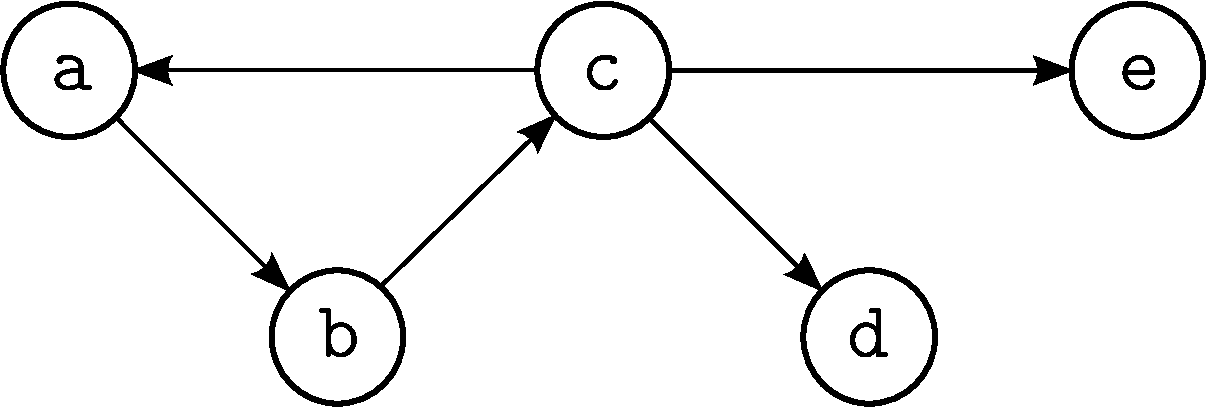
\includegraphics[width=0.5\textwidth]{cdg-loop.pdf}
\end{center}
\caption{带环的有向图}
\label{fig:a_directed_graph_with_a_loop}
\end{figure}

\begin{figure}
\begin{lstlisting}
(define (path node1 node2)
  (bf-path node2 (list (list node1))))

(define (bf-path dest queue)
  (if (null? queue)
      '@
      (let* ((path (car queue))
              (node (car path)))
         (if (eq? node dest)
             (cdr (reverse path))
             (bf-path dest
                      (append (cdr queue)
                              (map (lambda (n)
                                     (cons n path))
                                   (neighbors node))))))))
\end{lstlisting}
\caption{确定性搜索}
\label{fig:deterministic_search}
\end{figure}

从理论上说,非确定性应该可以让我们不用考虑环路带来的问题。
\ref{sec:scheme_implementation} 中给出
的~\emph{choose} 和~\emph{fail} 的深度优先实现是无法解决环路问题
的,但倘若我们当初要求更严格一些的话,那么应该会要求非确定性
的~\emph{choose} 能够依据任意可计算的指标来选择对象,所以这次的例子照
道理也应该不在话下。如果能用上正确版本的~\emph{choose}\index{nondeterministic choice 非确定性选择!correct 正确} 的话,我们就能像图~\ref{fig:nondeterministic_search} 中那样,写出更简短、更清晰的~\texttt{path}。


\begin{figure}
\begin{lstlisting}
(define (path node1 node2)
  (cond ((null? (neighbors node1)) (fail))
        ((memq node2 (neighbors node1)) (list node2))
        (else (let ((n (true-choose (neighbors node1))))
                (cons n (path n node2))))))
\end{lstlisting}
\caption{非确定性搜索}
\label{fig:nondeterministic_search}
\end{figure}

本节会给出一个环路安全的~\emph{choose} 和~\emph{fail} 的实现。
图~\ref{fig:correct_choose_in_scheme} 中真正\index{correct 真正的}的非
确定性~\emph{choose} 和~\emph{fail} 的~Scheme 实现对于环路也能正常
工作。\note{303}只要是等价的非确定性算法能处理的问题,使用了这个版本
的~\emph{choose} 和~\emph{fail} 的程序也一定能找到答案,不过这一点
还会受到硬件的限制。

\begin{figure}
\begin{lstlisting}
(define *paths* ())
(define failsym '@)

(define (true-choose choices)
  (call-with-current-continuation
    (lambda (cc)
      (set! *paths* (append *paths*
                            (map (lambda (choice)
                                   (lambda () (cc choice)))
                                 choices)))
      (fail))))

(define fail)

(call-with-current-continuation
  (lambda (cc)
    (set! fail
          (lambda ()
            (if (null? *paths*)
                (cc failsym)
                (let ((p1 (car *paths*)))
                  (set! *paths* (cdr *paths*))
                  (p1)))))))
\end{lstlisting}
\caption{\emph{choose} 的~Scheme 版正确实现}
\label{fig:correct_choose_in_scheme}
\index{true-choose@\texttt{true-choose}!breadth-first version}
\end{figure}

图~\ref{fig:correct_choose_in_scheme} 中定义的~\texttt{true-choose} 把
用来保存路径的列表当成一个队列来操作。因此,使用~\texttt{true-choose}
的程序对状态空间进行的搜索将是广度优先的\index{nondeterministic choice 非确定性选择!breath-first 广度优先}。每当程序到达选择点的时
候,与每一个选择相对应的续延都会被加入到用来保存路径的列表后
面。(Scheme 的~\texttt{map} 的返回值和~Common Lisp 的~\texttt{mapcar}
的返回值是一样的。) 然后,和之前一样,还是调用~\texttt{fail}。

如果用了这个版本
的~\emph{choose},图~\ref{fig:nondeterministic_search} 里定义
的~\texttt{path} 就能找到一条路径了,事实上,它找到的是最短路径,即
图~\ref{fig:a_directed_graph_with_a_loop} 中所示的
从~\texttt{a} 到~\texttt{e} 的那条路径。

虽然为了内容的完整性,本章给出了正确版本的~\emph{choose}
和~\emph{fail},其实最初的版本就够用了。我们不能仅仅因为其实现不是
形式上正确的,就低估编程语言所提供抽象机制的价值。在用一些语言编程的时
候,感觉上似乎我们能使用任意一个整数,其实能操作的最大一个整数可能只
是~32767。其实只要清楚幻象的限度,那么它所带来的危险就微不足道了,
至少我们的抽象是有保证的。下两章中程序的简洁明了,很大程度上就归功于它
们对非确定性~\emph{choose} 和~\emph{fail} 的善用。

%%% Local Variables:
%%% coding: utf-8
%%% mode: latex
%%% TeX-master: "onlisp-cn"
%%% End:

%!TEX encoding = UTF-8 Unicode
% $Id: 23-parsing_with_atns.tex 18 2014-03-12 22:35:24Z binghe $

\chapter{使用~ATN 分析句子}
\label{chap:parsing_with_atns}

这一章将介绍这样一种技术,它把非确定性分析器~(parser) \index{parsers,
  nondeterministic 分析器, 非确定性|see{ATNs}} 实现成一种嵌入式的语言。
其中,第一部分将会解释什么是~\textsc{ATN} 分析器,以及它们是如何表示语
法规则的。第二部分会给出一个~\textsc{ATN} 编译器,这个编译器将会使用在
前一章定义的非确定性操作符。最后的几个小节则会展示一个小型
的~\textsc{ATN} 语法,然后看看它在实际中是如何分析一段样本代码的。

\section{背景知识}
\label{sec:background}

扩充转移网络\index{augmented transition networks 扩充转移网
  络|see{ATNs}}~(\textsc{ATN})\index{ATNs},是~Bill Woods\index{Woods,
  William A.} 在~1970 年提出的一种分析器。在那之后,\textsc{ATN} 在自然语
言\index{natural language|see{\textsc{ATN}s}}\index{ATNs!for natural language 用于自然语言}分析领域中作为一种形式
化方法,被广为使用。\note{305} 只消一个小时,你就能写出一个能分析有意义
的英语句子的~\textsc{ATN} 语法。出于这个原因,人们常常在初次见识~\textsc{ATN} 之后,就
会为之着迷。

在~1970 年代,一部分研究者认为~\textsc{ATN} 有朝一日有可能会成为真正感觉有智能的
程序的一部分。尽管时至今日,还持有这一观点的人寥寥可数,不过~ATN 的地位
是不可磨灭的。它虽然没有你分析英语句子那么在行,但是它仍然能分析数量可
观的各种句子。

如果你恪守下面的四个限制条件,\textsc{ATN} 就能大显神通:

\begin{enumerate}
\item 仅限用于语义上有限制的领域,比如说作为某个特定的数据库前端。

\item 不能给它过于困难的输入。比如说,请不要认为它们能像人一样能理解非常
  没有语法的句子。

\item 它们仅仅适用于英语\index{English 英语},或者其他单词的顺序决定其语法结构的语言。比如
  说,\textsc{ATN} 就很可能无法被用来分析那种有屈折变化的语言\footnote{译者
    注:屈折语言~(inflected language),是语言学中的概念,指因为单词的变
    格造成语句本身结构和意思的变化。汉语和英语主要依靠单词的顺序来确定
    其语法结构,而屈折语言则主要根据单词的屈折变化~(inflection) 来表现
    句子中的语法关系,比如说拉丁语和德语。虽然英语不是屈折语言,但是它
    里面还是保留着一些形式的屈折变化。比如我们常见的人称代词的``格''的
    变化,主格的~he 和宾格的~him,属格的~his。它们的词根相同,但是词尾
    的变化导致了词性和意思的变化,但是其在句子中的位置仍是决定其意义的
    主要因素。},如拉丁语\index{Latin}。

\item 不要认为它们总是能正常工作。如果一个应用程序里,只要求它在~90\%的
  情况下正常工作就足够了,那么~\textsc{ATN} 是可以胜任的。倘若要求它不能出丝毫的
  差错,那么就不应该考虑用它。

\end{enumerate}
 
尽管有种种限制,\textsc{ATN} 还是能在很多地方派上用场。最典型的应用案例是用做数
据库的前端。如果你给这种数据库系统配备一个用~\textsc{ATN} 驱动的接口
\index{databases 数据库!natural language interfaces to 的自然语言接
  口},用户查询的时候就不用再构造特定格式的请求,只要用一种形式受限的英
语提问就可以了。

\section{形式化}
\label{sec:the_formalism}

要理解~\textsc{ATN} 的工作机制,我们首先要回忆一下它的全名:扩充转移网络~(Augmented Transition Network)\index{transition networks 转移网络}。所谓转
移网络,是指由有向弧连接起来的一组节点,从根本上可以把它看作一种流程图。
其中一个节点被指定为起始节点,而部分其他节点则被作为终结节点。每条弧上都
带有测试条件,只有对应的条件被满足的时候,状态才能经由这条弧转移到新
的节点。首先,输入是一个序列,并有一个指向当前单词的指针。根据弧进行状
态转移会使指针相应地前进。使用转移网络分析句子的过程,就是找到从起始节
点走到某个终止节点的路径的过程,在这个过程中,所有的转移条件都要满足。

\textsc{ATN} 在这个模型的基础上另加入了两个特性:

\begin{enumerate}

\item \textsc{ATN} 带有寄存器\index{ATNs!registers of 寄存器}。寄存器是有名字的~slot,它可以被用来保存分析过程中
  所需的有关信息。转移弧除了能进行条件判断之外,还会设置和修改寄存器中
  的内容。

\item \textsc{ATN} 的结构可以是递归的\index{ATNs!recursion in 递归}。转移弧可以这样要求:如果要通过这条弧,分
  析过程必须能通过某个子网络。

\end{enumerate}

而终结节点则使用寄存器中累积得到信息来建立列表结构并返回它,这种返回结
果的方式和函数返回值的方式非常像。实际上,除了它具有的非确定性之
外,\textsc{ATN} 的行为方式和函数式编程语言很相似。

图~\ref{fig:a_very_small_atn} 中定义的~\textsc{ATN} 几乎是最简单的~\textsc{ATN} 了。它
能分析形如``Spot runs''~(``电视广告插播中'') 的名词 -- 动词型句子。这
种~\textsc{ATN} 的网络表示如图~\ref{fig:graph_of_a_small_atn} 所示。

\begin{figure}
\begin{lstlisting}
(defnode s
  (cat noun s2
    (setr subj *)))

(defnode s2
  (cat verb s3
    (setr v *)))

(defnode s3
  (up '(sentence
         (subject ,(getr subj))
         (verb ,(getr v)))))
\end{lstlisting}
  \caption{一个微型~ATN}
  \label{fig:a_very_small_atn}
\end{figure}

\begin{figure}
\begin{center}
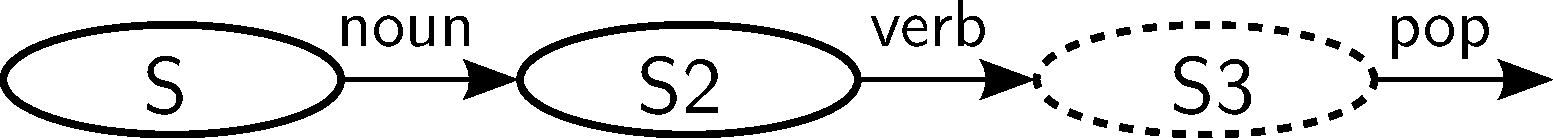
\includegraphics[width=.5\textwidth]{mini-atn.pdf}
\end{center}
  \caption{微型~ATN 的图示}
  \label{fig:graph_of_a_small_atn}
\end{figure}

当~\textsc{ATN} 分析输入序列~\texttt{(spot runs)} 时,它是如何工作的呢?第一个节
点有一条出弧~(outgoing arc),或者说一条类型弧~(cat),这条弧指向节
点~\texttt{s2}。这事实上是表示:如果当前单词是个名词的话,你就可以通过
我;如果你通过我的话,你必须把当前单词~(即~\texttt{*}) 保存
在~\texttt{subj} 寄存器中。因而,当离开这个节点时,
\verb|subj| 的内容就变成了~\verb|spot|。

总是有个指针指向当前的单词。在开始的时候,它指向句子的第一个单
词。在经过~cat 弧的时候,指针会往前移动一个单词。因此,在我们到
达~\texttt{s2} 节点的时候,当前节点会变成第二个单词,即~\texttt{runs}。
第二条弧线和第一条一样,不同之处在于它要求的是个动词。它发现
了~\texttt{runs},并把它保存在寄存器~\texttt{v} 里面,然后状态就走到
了~\texttt{s3}。

在最后一个节点~\texttt{s3} 上,只有一个~pop 弧~(或称为终止
弧)。(有~pop 弧的节点的外围线是虚线)。由于我们正好在把输入序列读完的时候
通过了~pop 弧,所以我们进行的句子分析是成功的。Pop 弧返回的是一个\bq\index{backquote@backquote (\texttt{`}) \bq!in ATNs}表达
式:

\begin{lstlisting}
(sentence (subject spot)
          (verb runs))
\end{lstlisting}

一个~\textsc{ATN} 是与它所要分析语言的语法相对应的。一个用来分析英语的~\textsc{ATN},如果
规模适中的话,那么它会有一个用来分析句子的主网络,以及用来分析名词短语、
介词短语,以及修饰词组等语法元素的多个子网络。让我们想一想含有介词短语
的名词短语,其中,介词短语也是有可能含有名词短语的,并且这种结构可能
会\emph{无穷无尽}地延续下去。显而易见,要处理下面这种结构的句子,必须
要能支持递归:

\begin{quote} 
  ``the key on the table in the hall of the house on the hill''
\end{quote}

\section{非确定性}
\label{sec:nondeterminism}

尽管我们在这个简单的例子里面没有看出来,但是~\textsc{ATN} 的确是非确定性的。一个
节点可以有多个出弧,而特定的输入可以同时满足一个以上的出弧的条件。举个
例子,一个像样的~\textsc{ATN} 应该既能分析祈使句也能分析陈述句。所以第一个节点要
有向外的~cat 弧,与名词~(用于陈述句) 和动词~(用于祈使句)。

要是句子开头的单词是``time''呢?``time''既是名词又是动词。分析器如何知
道该选哪条弧呢?如果~\textsc{ATN} 是以不确定的方式\index{ATNs!nondeterminism in}运行的,那就意味着用户可以认为
分析器总是会\emph{猜到正确的}那条弧线。如果有弧线会让分析过程走进死胡同,那么它们
是不会被选中的。

实际上,分析器是无法预见未来的。它只是在无路可走,或者读完了输入还没能
结束分析时,通过回溯的方式来表现出老是猜中的表象。不过所有这些回溯的机
制是自动嵌入在~\textsc{ATN} 编译器产生的代码里面的。所以,在编写~\textsc{ATN} 时,我们可
以认为分析器能够猜出来应该选择哪一条弧通过。

就像许多~(也许是绝大多数) 使用非确定性算法的程序所做的那样,\textsc{ATN} 一样,
使用的也是深度优先搜索\index{nondeterministic choice 非确定性选择!depth-first 深度优先!in ATNs@in \textsc{ATN}s}。如果曾有过分析英语的经验,就能很快了解到,任何
句子都有大把的合法分析结果,但是它们中的绝大多数都是没有意义的。在传统
的单处理器电脑上,一样可以迅速得到较好的分析结果。我们不是一下子算出所
有的分析结果,而只是得出最有可能的那个。如果分析结果是合理的,那么我们
就用不着再去搜索其他的分析方式了;否则我们还可以调用~\emph{fail} 继续
搜寻更多其它的方式。

为了控制生成分析结果的先后顺序,程序员需要借助某种办法来控
制~\emph{choose} 尝试各待选项的顺序。深度优先实现并不是唯一一种控制搜
索顺序的办法。除非选择是随机的,否则任意一种实现都会按照其特定的顺序进
行选择。不过,\textsc{ATN} 和~Prolog 一样,深度优先实现是其内化了的实现方式。
在~\textsc{ATN} 中,出弧被选中的顺序就是它们当初被定义的顺序\index{ATNs!order of arcs 转移弧的顺序}。使用这样的设计,程
序员就可以根据优先级来排列转换弧线的定义了。

\section{一个~\textsc{ATN} 编译器}
\label{sec:an_atn_compiler}
\index{embedded languages!ATNs as@\textsc{ATN}s as}
一般来说,一个基于~\textsc{ATN} 的分析器由三个部分组成:\textsc{ATN} 本身、用来遍历这个~\textsc{ATN}
的解释器,还有一个可以用于查询的词典。举个例子,借助词典我们就可以知道
``run''是个动词。说到词典,那是另一个话题了,我们在这里会使用一个比较初
级的手工编制的词典。我们也不用在网络解释器上费心,因为我们会把~\textsc{ATN} 直接
翻译成~Lisp 代码。在这里要介绍的程序被称为~\textsc{ATN} 编译器的原因是,这个程序
能把整个的~\textsc{ATN} 变成对应的代码。节点会成为函数,而转换弧则会变成函数里的
代码块。

第~\ref{chap:functions_as_representation} 章介绍了把函数作为表达方式的用法\index{ATNs!represented as functions 函数作为表达方式}。
这种编程习惯常常能让程序的运行速度更快。在这里,这意味着会免去在运行时
解析网络的开销。而这样处理的缺点在于,如果出了问题的话,分析原因的线索就会更少了,特别
是如果你用的~Common Lisp 实现没有提供~\texttt{function-lambda-expression} 
\footnote{译者注:见~\emph{CLHS} 中 ~\href{http://www.lisp.org/HyperSpec/Body/fun_function-_a-expression.html}{Function
    FUNCTION-LAMBDA-EXPRESSION} 一节。}的时候.

图~\ref{fig:compilation_of_nodes_and_arcs} 中包含了所有用来把~\textsc{ATN} 节点
转换为~Lisp 代码的源程序。其中~\texttt{defnode} 宏被用来定义节点。它本
身生成的代码很有限,就是一个~\texttt{choose},用来在每个转换弧产生的表
达式中进行选择。节点函数有两个参数,分别是~\texttt{pos} 和~\texttt{regs}:
\texttt{pos} 的值是当前的输入指针~(一个整数),而~\texttt{regs} 是当前的
寄存器组~(为一个关联表的列表)。

\begin{figure}
\begin{lstlisting}
(defmacro defnode (name &rest arcs)
  `(=defun ,name (pos regs) (choose ,@arcs)))

(defmacro down (sub next &rest cmds)
  `(=bind (* pos regs) (,sub pos (cons nil regs))
          (,next pos ,(compile-cmds cmds))))

(defmacro cat (cat next &rest cmds)
  `(if (= (length *sent*) pos)
       (fail)
       (let ((* (nth pos *sent*)))
         (if (member ',cat (types *))
             (,next (1+ pos) ,(compile-cmds cmds))
             (fail)))))

(defmacro jump (next &rest cmds)
  `(,next pos ,(compile-cmds cmds)))

(defun compile-cmds (cmds)
  (if (null cmds)
      'regs
      `(,@(car cmds) ,(compile-cmds (cdr cmds)))))

(defmacro up (expr)
  `(let ((* (nth pos *sent*)))
     (=values ,expr pos (cdr regs))))

(defmacro getr (key &optional (regs 'regs))
  `(let ((result (cdr (assoc ',key (car ,regs)))))
     (if (cdr result) result (car result))))

(defmacro set-register (key val regs)
  `(cons (cons (cons ,key ,val) (car ,regs))
	 (cdr ,regs)))

(defmacro setr (key val regs)
  `(set-register ',key (list ,val) ,regs))

(defmacro pushr (key val regs)
  `(set-register ',key
                 (cons ,val (cdr (assoc ',key (car ,regs))))
                 ,regs))
\end{lstlisting}
  \caption{节点和弧的编译}
  \label{fig:compilation_of_nodes_and_arcs}
\end{figure}

宏~\texttt{defnode} 定义了一个宏,这个宏的名字和对应的节点相同。节
点~\texttt{s} 将会被定义成宏~\texttt{s}。这种习惯做法让转换弧知道
如何引用它们的目标节点 \pozhehao{} 它们只要调用和节点同名的宏就可以了。这
同时也意味着,你在给节点取名的时候应该避免和已有的函数或者宏重名,否则
这些函数或宏会被重定义。

调试~\textsc{ATN} 时,需要借助某种~trace\index{ATNs!tracing} 工具。由于节点成为了
函数,所以就用不着自己实现~trace 了。我们可以利用内建的~Lisp 函
数~\verb|trace|\index{trace@\texttt{trace}}。如同第~\pageref{trace} 页
提到的,只要用~\verb|=defun| 定义节点,就意味着我们可以通过告诉~Lisp
\verb|(trace =mods)| 来对节点~\verb|mods| 的分析过程进行~trace。

节点函数体里面的转移弧就是宏调用,而宏调用返回的代码被嵌入
在~\texttt{defnode} 生成的节点函数中。因此,每个节点的出弧都被表示为对
应的代码,分析器每碰到一个节点,都会通过执行~\texttt{choose} 使用非确定
性的机制来对这些代码择一执行。比如下面这个有几条出弧的节点
\begin{lstlisting}
(defnode foo
  <arc 1>
  <arc 2>)
\end{lstlisting}
就会被变换成如下形式的函数定义:
\begin{lstlisting}
(=defun foo (pos regs)
  (choose
    <translation of arc 1>
    <translation of arc 2>))
\end{lstlisting}

\begin{figure}
\begin{lstlisting}
(defnode s
  (down np s/subj
    (setr mood 'decl)
    (setr subj *))
  (cat v v
    (setr mood 'imp)
    (setr subj '(np (pron you)))
    (setr aux nil)
    (setr v *)))
\end{lstlisting}
被宏展开成:
\begin{lstlisting}
(=defun s (pos regs)
  (choose
    (=bind (* pos regs) (np pos (cons nil regs))
      (s/subj pos
              (setr mood 'decl
                    (setr subj * regs))))
    (if (= (length *sent*) pos)
        (fail)
        (let ((* (nth pos *sent*)))
          (if (member 'v (types *))
              (v (1+ pos)
                 (setr mood 'imp
                       (setr subj '(np (pron you))
                             (setr aux nil
                                   (setr v * regs)))))
              (fail))))))
\end{lstlisting}
  \caption{节点函数的宏展开}
  \label{fig:macroexpansion_of_a_node_function}
\end{figure}

图~\ref{fig:macroexpansion_of_a_node_function} 显示了
图~\ref{fig:sentence_network} 中作为~\textsc{ATN} 例子里第一个节点的宏展开前后的
模样。当节点函数~(如~\texttt{s}) 在运行时被调用时,会非确定性地选择一条
转移弧通过。\texttt{pos} 参数将会是在输入句子中的当前位
置,而~\texttt{regs} 则是现有的寄存器数据。

\index{ATNs!arc types 转移弧的种类}
就像在我们最初的那个例子中见到的,cat 弧要求当前的输入单词在语法上属于
某个类型。在~cat 弧的函数体中,符号~\texttt{*} 将会被绑定到当前的输入单
词上。

%% xxx
由~\texttt{down} 定义的~push 弧,则要求对子网络的调用能成功返回。这些弧
函数接受两个目标节点作为参数,它们分别是:子网络目标节
点~\texttt{sub},和当前网络的下个节点,即~\texttt{next}。注意到,虽然
为~cat 弧生成的代码只是调用了网络中的下一个节点,但是为~push 弧生成的代
码使用的是~\texttt{=bind}。在继续转移到~push 弧指向的节点前,程序必须成
功地从子网络返回。 在~\texttt{regs} 被传入子网络前,一组新的空寄存
器~(\texttt{nil})\index{stacks 栈!of ATN registers} 被~cons 到它的前面。在其他类型的转移弧的函数体中,符
号~\texttt{*} 将会被绑定到输入的当前单词上,不过
在~push 弧中,\texttt{*} 则是被绑定到从子网络返回的表达式上。


jump 弧就像发生了短路一样。分析器直接跳到了目标节点,不需要进行条件测
试,同时输入指针没有向前移动。

最后一种转移弧是~pop 弧,这种转移弧由~\texttt{up} 定义。pop 弧是比较不
常见的,原因在于它们没有目标节点。就像~Lisp 的~\texttt{return} 类
似,\texttt{return} 把程序带到的不是一个子函数,而是主调函数,而~pop
弧指向的不是一个新节点,而是把程序带回``调用方''的~push 弧。pop 弧
的~\texttt{=values} ``返回''的是最近的一个~push 弧的~\texttt{=bind}。但
是如第~\ref{sec:the_formalism} 节所述,这产生的结果和一个普通的~Lisp
\texttt{return} 还不一样,\texttt{=bind} 的函数体已经被包在一
个\continuation{}里了,并且被作为参数顺着之后的转移弧一直传下
去,直到~pop 弧的~\texttt{=values} 把``返回''值作为参数调用这个\continuation{}。

第~\ref{chap:nondeterminism} 章描述的两个版本的非确定
性~\emph{choose},分别是:一个快速的~\texttt{choose}
(第~\pageref{fig:scheme_implementation_of_choose_and_fail} 页),虽然它
无法保证在搜索空间里有环的情况下能正常终止;以及一个较慢
的~\texttt{true-choose} (第~\pageref{fig:correct_choose_in_scheme} 页),它
能在有环的情况下仍然正常工作。当然,在一个~\textsc{ATN} 同样有可能存在环,不过只
要在每个环里至少有一个转移弧能推进输入指针,那么分析器迟早都会走到句子
末尾。问题是出在那种不会推进输入指针的那种环上。这里我们有两个方案:
\begin{enumerate}
\item 使用较慢的、真正的非确定性选择操作
  符~(第~\pageref{func:true-choice} 页给出了其深度优先版本)。
\item 使用快速的~\texttt{choose},同时指出:如果定义的网络含有只需要顺
  着~jump 弧就能遍历的环,那么这个定义是错误的\index{ATNs!correctness of 的正确性}。
\end{enumerate}
在图~\ref{fig:compilation_of_nodes_and_arcs} 采用的是第二个方案。

图~\ref{fig:compilation_of_nodes_and_arcs} 中的最后四个定义定义了用来读
取和设置转移弧函数体中寄存器的宏。在这个程序里,寄存器组是用关联表来表
示的。\textsc{ATN} 所使用的并不是寄存器组,而是一系列寄存器组。当分析器进入一个
子网络时,它获得了一组新的空寄存器,这组寄存器被压在了已有寄存器组的上
面。因此,无论何时,所有寄存器构成的集合都是作为一个关联表的列表存在的。

这些预先定义好的寄存器操作符的操作对象都是当前,或者说是最上面的那一组
寄存器: \texttt{getr} 读一个寄存器;\texttt{setr} 设置寄存
器;而~\texttt{pushr} 把一个值加入寄存器。\note{312}
\texttt{setr}\footnote{译者注:原文为~\texttt{getr},根据上下文应
为~\texttt{setr}。}和~\texttt{pushr} 都使用了更基本的寄存器操作
宏:\texttt{set-register}。注意到,寄存器不需要事先声明。不管传
给~\texttt{set-register} 的是什么名字,它都会用这个名字新建一个寄存器。

这些寄存器操作符都是完全非破坏性的。
``Cons,cons,cons'',\texttt{set-register} 念念有词。
这拖慢了操作符运行的速度,同时也产生了大量无用的垃圾。不过,正如
第~\pageref{share-between-continuations} 页解释的,如果程序某一部分构造了一个\continuation{},那
么就不应该破坏性地修改在这个部分用到的对象\index{ATNs!destructive operations in 破坏性的操作}。一个正在运行的线程中的对象
有可能被另一个正被挂起的线程共享。在本例中,在一个分析过程中发现的寄存
器会与许多其他分析过程共享数据结构。如果速度成了问题,我们可以把寄存器
保存在~vector\index{vectors 向量!for ATN registers 用于~ATN 的寄存器} 里面,而不是关联表里,并且把用过的~vector 回收到一个公用
的~vector 池\index{pools 池}中。

push、cat 和~jump 弧都可以包含表达式体。通常情况下,这些表达式只不过会
是一些~\texttt{setr} 罢了。通过对它们的表达式体调
用~\texttt{compile-cmds},这些几类转移弧的展开函数会把一系
列~\texttt{setr} 串在一起,成为一个单独的表达式:
\begin{lstlisting}
> (compile-cmds '((setr a b) (setr c d)))
(SETR A B (SETR C D REGS))
\end{lstlisting}
每个表达式把它后面的那个表达式作为它的最后一个参数安插到自己的参数列表
中,不过最后一个表达式除外,它就是~\texttt{regs}。因此转移弧的函数体中
的一系列表达式就会被转换成一个单独的表达式,这个表达式将会返回新的那些
寄存器。

这个办法让用户能在转移弧的函数体里安插任意的~Lisp 代码,只要把这
些~Lisp 代码用一个~\texttt{progn} 包起来就可以了。举例来说:

\begin{lstlisting}
> (compile-cmds '((setr a b)
                        (progn (princ "ek!"))
                        (setr c d)))
(SETR A B (PROGN (PRINC "ek!") (SETR C D REGS)))
\end{lstlisting}

我们有意让转移弧的函数体中的代码能访问到部分变量。被分析的句子将被放到
全局的~\texttt{*sent*} 里。还有两个词法变量也将是可见的,它们
是:\texttt{pos},它保存着当前的输入指针;以及~\texttt{regs},它被用来
存放当前的所有寄存器。这是又一个有意地利用变量捕捉\index{capture 捕捉!intentional}的实例。如果期望让用
户不能引用这些变量,可以考虑把它们换成\gensym。

宏~\texttt{with-parses} 是在图~\ref{fig:atn:toplevel_macro} 中定义的,它让
我们有个办法能调用~\textsc{ATN}。要调用它,我们应该传给它起始节点的名字、一个需
要分析的表达式,以及一个代码体。这段代码告诉~\texttt{with-parses} 应该
如何处理返回的分析结果。表面上,\texttt{with-parses} 的功能
和~\texttt{dolist} 这种操作符差不多。实际上,在它内部进行的并不是简单的
叠代操作,而是回溯搜索。每次成功的分析动作都会引起
对~\texttt{with-parses} 表达式中的代码体的一次求值。在代码体中,符
号~\texttt{parse} 将会绑定到当前的分析结果上。\texttt{with-parses} 表达
式会返回~\texttt{@},因为这正是~\texttt{fail}在穷途末路时的返回值。

\begin{figure}
\begin{lstlisting}
(defmacro with-parses (node sent &body body)
  (with-gensyms (pos regs)
    `(progn
       (setq *sent* ,sent)
       (setq *paths* nil)
       (=bind (parse ,pos ,regs) (,node 0 '(nil))
         (if (= ,pos (length *sent*))
             (progn ,@body (fail))
             (fail))))))
\end{lstlisting}
  \caption{toplevel 宏}
  \label{fig:atn:toplevel_macro}
\end{figure}

在进一步研究表达能力更强的~\textsc{ATN} 之前,让我们先看一下之前定义的一个微
型~\textsc{ATN} 产生的分析结果。\textsc{ATN} 编译
器~(图~\ref{fig:compilation_of_nodes_and_arcs}) 产生的代码会调
用~\texttt{types},通过它了解单词的在语法上所担当的角色,所以我们需要先
给它下个定义:
\begin{lstlisting}
(defun types (w)
  (cdr (assoc w '((spot noun) (runs verb)))))
\end{lstlisting}

现在我们只要把起始节点作为第一个参数传给~\texttt{with-parses},并调用它:
\begin{lstlisting}
> (with-parses s '(spot runs)
    (format t "Parsing: ~A~%" parse))
Parsing: (SENTENCE (SUBJECT SPOT) (VERB RUNS))
@
\end{lstlisting}

\section{一个~\textsc{ATN} 的例子}
\label{sec:a_sample_atn}

既然我们把~\textsc{ATN} 编译器从头到尾都说清楚了,接下来可以找个例子小试牛刀了。
为了让~\textsc{ATN} 的分析器能处理的句子的类型更多些,你需要把~\textsc{ATN} 网络,而不
是~\textsc{ATN} 编译器弄得更复杂一些。这里展示的编译器之所以还只是个玩具,其原因
是因为它的速度比较慢,而不是它在处理能力上的局限性。

分析器的处理能力~(与处理速度相区别) 源自于它的语法,由于这里篇幅的限
制,所以我们不得不用一个玩具版本来说明问题。从图~\ref{fig:sub-network_for_strings_of_modifiers} 到
图~\ref{fig:sentence_network} 定义了图~\ref{fig:graph_of_a_larger_atn} 中所示的~\textsc{ATN} (或者说一
组~\textsc{ATN})。这个网络的规模正好足够大,使得它能在分析那句经典的分析素
材``Time flies like an arrow''时,能够得出多种分析结果。

\begin{figure}
\begin{center}
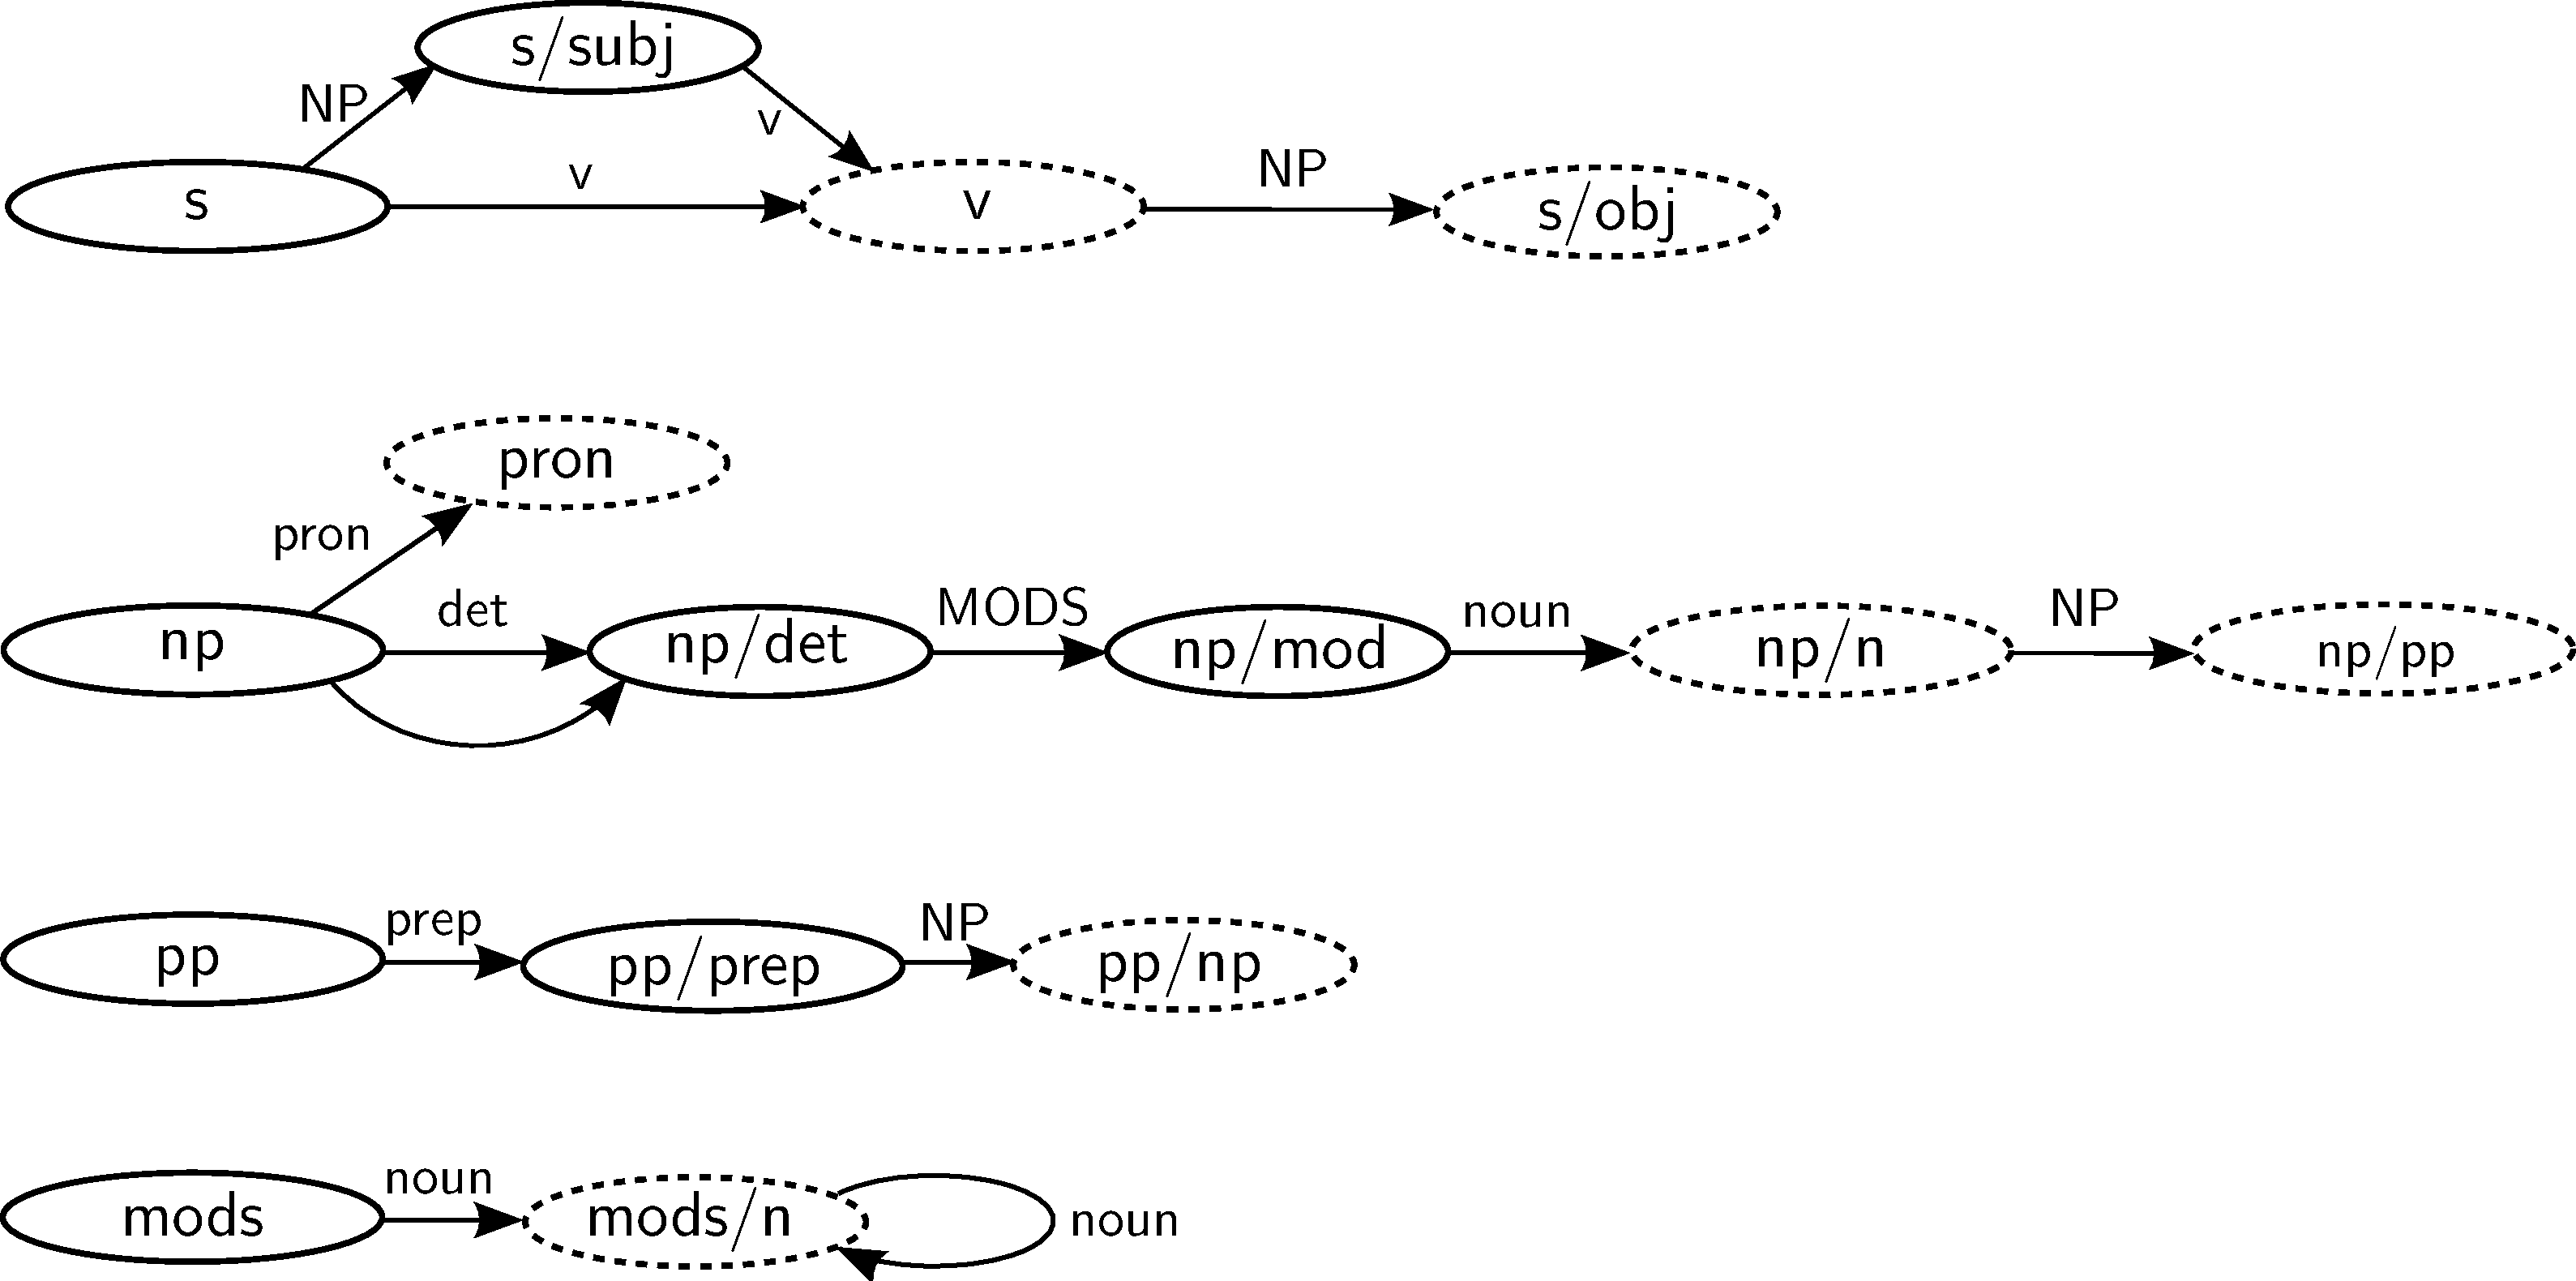
\includegraphics[width=\textwidth]{larger-atn.pdf}
\end{center}
  \caption{一个规模更大的~ATN}
  \label{fig:graph_of_a_larger_atn}
\end{figure}


\begin{figure}
\begin{lstlisting}
(defun types (word)
  (case word
    ((do does did) '(aux v))
    ((time times) '(n v))
    ((fly flies) '(n v))
    ((like) '(v prep))
    ((liked likes) '(v))
    ((a an the) '(det))
    ((arrow arrows) '(n))
    ((i you he she him her it) '(pron))))
\end{lstlisting}
  \caption{象征性的词典}
  \label{fig:nominal_dictionary}
\end{figure}

如果要分析更复杂的输入的话,我们就需要一个稍大的词典。函
数~\texttt{types} (图~\ref{fig:nominal_dictionary}) 提供了一个最基本的词典。它里面定义了
一个由~22 个词组成的词汇库,同时把每个词都和一个列表相关联,列表由一个
或多个单词对应的语法角色构成。


\begin{figure}
\begin{lstlisting}
(defnode mods
  (cat n mods/n
    (setr mods *)))

(defnode mods/n
  (cat n mods/n
    (pushr mods *))
  (up `(n-group ,(getr mods))))
\end{lstlisting}
  \caption{修饰词字符串的子网络}
  \label{fig:sub-network_for_strings_of_modifiers}
\end{figure}

\begin{figure}
\begin{lstlisting}
(defnode np
  (cat det np/det
    (setr det *))
  (jump np/det
    (setr det nil))
  (cat pron pron
    (setr n *)))

(defnode pron
  (up '(np (pronoun ,(getr n)))))

(defnode np/det
  (down mods np/mods
    (setr mods *))
  (jump np/mods
    (setr mods nil)))

(defnode np/mods
  (cat n np/n
    (setr n *)))

(defnode np/n
  (up '(np (det ,(getr det))
           (modifiers ,(getr mods))
           (noun ,(getr n))))
  (down pp np/pp
    (setr pp *)))

(defnode np/pp
  (up '(np (det ,(getr det))
           (modifiers ,(getr mods))
           (noun ,(getr n))
           ,(getr pp))))
\end{lstlisting}
  \caption{名词短语子网络}
  \label{fig:noun_phrase_sub-network}
\end{figure}

\textsc{ATN} 也是由~\textsc{ATN} 本身连接而成的。在本例中,我们的~\textsc{ATN} 部件中最小的一个是
图~\ref{fig:sub-network_for_strings_of_modifiers} 中的~\textsc{ATN}。它分析的是修饰语的字符串,在这里,指的就是名词
的字符串。\texttt{mods} 是第一个节点,它接受一个名词。第二个节点
是~\texttt{mods/n},它会去寻找更多的名词或者返回一个分析结果。

第~\ref{sec:functions_as_properties} 节介绍了把程序写成函数式风格能让程
序更易于测试的缘由:
\begin{enumerate}
\item 在函数式程序中,可以单独地测试程序的组成部件。
\item 在~Lisp 中,可以在~toplevel 的循环里交互地测试函数。
\end{enumerate}

这两条原因合在一起,成为了我们能进行\emph{交互式开发}\index{interactive development}的理由:当我们用~Lisp 写
函数式程序的时候,我们就可以每写一部分代码,就测试它们。

\textsc{ATN} 和函数式程序非常相像\index{ATNs!like functional programs 和函数式程序相像},从它的实现上看,\textsc{ATN} 宏展开\emph{成了}函数式的程序。
这个相似点使得交互式的开发方式也一样适用于~\textsc{ATN} 的开发。我们可以把任意一
个节点作为起点来测试~\textsc{ATN},只要把节点的名字作为~\texttt{with-parses} 的
第一个参数传入:

\begin{lstlisting}
> (with-parses mods '(time arrow)
        (format t "Parsing: ~A~%" parse))
Parsing: (N-GROUP (ARROW TIME))
\end{lstlisting}
接下来的两个网络需要放在一起讨论,因为它们之间是互相递归调用的。
图~\ref{fig:noun_phrase_sub-network} 中定义的网络被用来分析名词短语,它从节点~\texttt{np} 开始。
在图~\ref{fig:prepositional_phrase_sub-network} 中定义的网络则被用来分析介词短语。名词短语有可能含有介
词短语,反之亦然。所以它们两个各自有一个~push 弧,分别调用另一个网络。

名词短语网络中有六个节点。其中,第一个节点~\texttt{np} 有三个选择。如果
它读到了一个代词,那么它就可以转移到节点~\texttt{pron},这会让它弹出这
个网络:
\begin{lstlisting}
> (with-parses np '(it)
    (format t "Parsing: ~A~%" parse))
Parsing: (NP (PRONOUN IT))
@
\end{lstlisting}

另外两个转移弧都指向了节点~\texttt{np/det}:一条弧读入一个限定词~(比如
说~``the''),而另一条弧则直接跳转,不从输入读取任何词。在节
点~\texttt{np/det},两条出弧都通向~\texttt{np/mods};\texttt{np/det} 可
以选择~push 到子网络~\texttt{mods},以此来找出修饰词的字串,或者直
接~jump。节点~\texttt{np/mods} 读入一个名词,然后转移到~\texttt{np/n}。
这个节点要么弹出结果,要么进入介词短语网络,看看能不能碰到个介词短语。
最后的节点,即~\texttt{np/pp},弹出结果。

分析不同类型的名词短语所走过分析路径也各不相同。下面是两个名词短语网络
的分析结果:
\begin{lstlisting}
> (with-parses np '(arrows)
    (pprint parse))
(NP (DET NIL)
    (MODIFIERS NIL)
    (NOUN ARROWS))
@
> (with-parses np '(a time fly like him)
        (pprint parse))
(NP (DET A)
    (MODIFIERS (N-GROUP TIME))
    (NOUN FLY)
    (PP (PREP LIKE)
        (OBJ (NP (PRONOUN HIM)))))
@
\end{lstlisting}

第一次分析在最后~jump 到~\texttt{np/det},再~jump 到~\texttt{np/mods}
读入一个名词,然后~pop 到~\texttt{np/n},从而成功结束。第二次的尝试过程
中没有~jump 过,它首先为了匹配一个修饰词字符串~push 进一个子网络,然后
为了介词短语也进入了一个子网络。这应该是分析器的通病,我们的分析器也不
例外:有些在句法上没有问题的表述在语义上却毫无意义,以致于人都没有办法
看出它们的句法结构。这里,名词短语``a time fly like him''和``a Lisp
hacker like him''的形式就是一样的。

\begin{figure}
\begin{lstlisting}
(defnode pp
  (cat prep pp/prep
    (setr prep *)))
(defnode pp/prep
  (down np pp/np
    (setr op *)))
(defnode pp/np
  (up ‘(pp (prep ,(getr prep))
           (obj ,(getr op)))))
\end{lstlisting}
  \caption{介词短语子网络}
  \label{fig:prepositional_phrase_sub-network}
\end{figure}


\begin{figure}
\begin{lstlisting}
(defnode s
   (down np s/subj
       (setr mood 'decl)
       (setr subj *))
   (cat v v
       (setr mood 'imp)
       (setr subj '(np (pron you)))
       (setr aux nil)
       (setr v *)))

(defnode s/subj
  (cat v v
    (setr aux nil)
    (setr v *)))

(defnode v
  (up `(s (mood ,(getr mood))
          (subj ,(getr subj))
          (vcl (aux ,(getr aux))
               (v ,(getr v)))))
  (down np s/obj
    (setr obj *)))

(defnode s/obj
  (up `(s (mood ,(getr mood))
          (subj ,(getr subj))
          (vcl (aux ,(getr aux))
               (v ,(getr v)))
          (obj ,(getr obj)))))
\end{lstlisting}
  \caption{句子网络}
  \label{fig:sentence_network}
\end{figure}

万事俱备,只欠东风。现在我们缺的就是一个能识别整句结构的网络了。
图~\ref{fig:sentence_network} 中的网络同时能分析祈使句和陈述句。按照习
惯,起始节点被叫做~\texttt{s}。第一个节点首先从一个名词短语开始。第二条
出弧读入一个动词。当句子在句法结构上有歧义时,两条转移弧都可能被满
足,最终得到两个或更多的分析结果,如
图~\ref{fig:two_parsings_for_a_sentence} 所示。第一个分析结果
和``Island nations like a navy''类似,而第二个和``Find someone like a
policeman''是同一种。对于``Time flies like an arrow'',更复杂的~\textsc{ATN} 能找
出六种以上的分析结果。

\begin{figure}
\begin{lstlisting}
> (with-parses s '(time flies like an arrow)
    (pprint parse))
(S (MOOD DECL)
   (SUBJ (NP (DET NIL)
             (MODIFIERS (N-GROUP TIME))
             (NOUN FLIES)))
   (VCL (AUX NIL)
        (V LIKE))
   (OBJ (NP (DET AN)
            (MODIFIERS NIL)
            (NOUN ARROW))))
(MOOD IMP)
   (SUBJ (NP (PRON YOU)))
   (VCL (AUX NIL)
        (V TIME))
   (OBJ (NP (DET NIL)
            (MODIFIERS NIL)
            (NOUN FLIES)
            (PP (PREP LIKE)
                (OBJ (NP (DET AN)
                         (MODIFIERS NIL)
                         (NOUN ARROW)))))))
@
\end{lstlisting}
  \caption{一个句子的两种分析方式}
  \label{fig:two_parsings_for_a_sentence}
\end{figure}

在这一章给出~\textsc{ATN} 编译器的目的更多的在于展示如何提炼出一个~\textsc{ATN} 思路的精
髓,而不是实现一个产品级的软件。如果进行一些很明显的改进,代码的效率就
能显著提升。当速度很重要的时候,用闭包来模拟非确定性这个思路从整体上
说,也许就太慢了。但是如果速度不是关键问题,用本章介绍的这种编程技术可
以写出十分简洁明了的程序。


%%% Local Variables:
%%% coding: utf-8
%%% mode: latex
%%% TeX-master: "onlisp-cn"
%%% End:

%!TEX encoding = UTF-8 Unicode
% $Id: 24-prolog.tex 18 2014-03-12 22:35:24Z binghe $

\chapter{Prolog}
\label{chap:prolog}
\index{Prolog}

本章将介绍如何编写嵌入式的~Prolog 解释器。
第~\ref{chap:a_query_compiler} 章中已经展示了编写数据库查询语
句编译器的方法,这里我们再加入一个新的元素\index{Prolog!conceptual ingredients}:规则。有了规则,就可以根据已有的知识
通过推理得到新知。
一组规则定义了表明事实之间相互蕴含关系的一棵树。由于这棵树可能包含无限多的事实,所以我们必须使用非确定性的搜索。

Prolog 是嵌入式语言的一个极好的例子。它融合了三个元素:模式匹配,非确定性,
规则。其中,前两个元素在第~\ref{chap:destructuring} 章和
第~\ref{chap:nondeterminism} 章曾分别介绍过。把~Prolog 建立在
模式匹配和非确定性选择操作的基础之上,我们可以得到一个真正的,多层的,自底向
上的系统\index{bottom-up design 自底向上的设计!multilayer 多层的}。图~(\ref{fig:layers_of_abstraction}) 展示了有关几个抽象层的结构。

\begin{figure}
  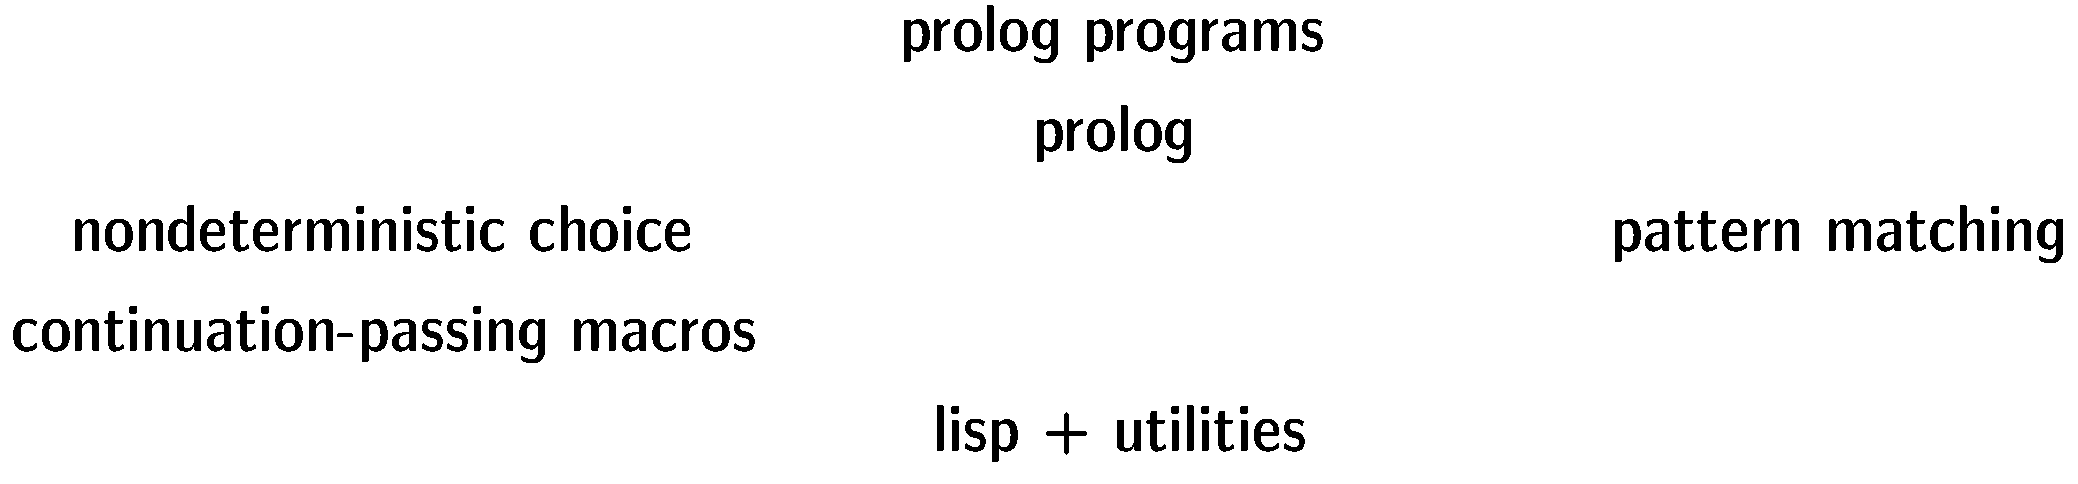
\includegraphics[width=.98\textwidth]{layers.pdf}
  \caption{抽象层}
  \label{fig:layers_of_abstraction}
\end{figure}

本章的第二个目标是学习~Prolog。对于经验丰富的程序员来说,简要地说明一
下其实现方式可能会更有助于讲解这门语言。而用~Lisp 实现~Prolog 非常有趣,因为
在这过程中能够发掘出这两者间的共同点。


\section{概念}
\label{sec:prolog:concepts}

第~\ref{chap:a_query_compiler} 章介绍了如何写一个能接受复杂查询语句的
数据库系统,这个系统能自动生成所有满足查询条件的绑定。在下例中,(调
用~\verb|clear-db| 之后),我们声明两个事实,然后对数据库进行查询:
\begin{lstlisting}
> (fact painter reynolds) 
(REYNOLDS) 
> (fact painter gainsborough) 
(GAINSBOROUGH) 
> (with-answer (painter ?x) 
    (print ?x)) 
GAINSBOROUGH 
REYNOLDS 
NIL 
\end{lstlisting}

从概念上说,Prolog~是一个~``附有规则的数据库程序''。它不仅仅能够直接从
数据库中查找匹配的数据来满足查询语句,还能够从已知的事实~(数据) 中推导
出匹配的数据。例如,若有如下的规则:

\prule
{\texttt{(hungry ?x)} and \texttt{(smells-of ?x turpentine)}}
{\texttt{(painter ?x)}}
则,只要数据库中存在~\texttt{(hungry raoul)} 和~\texttt{(smells-of raoul
  turpentine)} 这两个事实,那么~\texttt{?x = raoul} 就能满足查询语
句~\texttt{(painter ?x)},即使数据库中没有~\texttt{(painter raoul)}
这个事实。

在~Prolog 中,规则的~``if'' 部分被称作~\emph{body}\index{body (of a rule)},``then'' 部分被称
作~\emph{head}。(在逻辑中,它们分别叫做\emph{前提}~(\emph{antecedent})\index{antecedent 前提,前
件,先决条件} 和\emph{推论}~(\emph{consequent})\index{consequent 推论,结果},不过用不同的名字也好,
能强调~Prolog 的推导不同于逻辑的推导)。在我们试图生成查询的绑定
时\footnote{这章的许多概念,比如~binding 的含义,在
  第~\ref{sec:destructuring:matching} 节已经说明。},
程序首先检查规则的~head,如果~head 能满足查询,那么程序会做出
响应,为~body 建立各种绑定。根据定义,如果绑定满足~body,
那么它也满足~head。\index{rules!structure of}

在规则的~\emph{body} 中用到的各种事实可能会转而由其他规则中推演得出。例如:

\prule
{\texttt{(gaunt ?x)} or \texttt{(eats-ravenously ?x)}}
{\texttt{(hungry ?x)}}
规则也可以是递归的,例如:

\prule
{\texttt{(surname ?f ?n)} and \texttt{(father ?f ?c)}}
{\texttt{(surname ?c ?n)}}

如果~Prolog 能在种种规则中找到一条通往已知事实的路径,它便会为该查询建立各
种绑定。因而,它实质上是一个搜索引擎:它遍历由各种规则形成的逻辑蕴含树,
寻找一条通往事实的成功之路。

虽然规则和事实听上去像两回事,其实它们在概念上是可以互
换的\pozhehao{}规则可以被看作虚拟事实\index{rules!as virtual facts}。如果我们希望我们的数据库能够反映出
“凶猛的大型动物是稀有的”这个发现,我们可以寻找所有
的~\emph{x},令~\emph{x} 满足~\texttt{(species $x$)},\texttt{(big
  $x$)} 和~\texttt{(fierce $x$)} 这些事实,找到的话就加上一个新的事实~\texttt{(rare
  $x$)}。如果定义下面的规则:
\prule
{\texttt{(species ?x)} and \texttt{(big ?x)} and \texttt{(fierce ?x)}}
{\texttt{(rare ?x)}}
就会得到相同的效果,而无需在数据库中加入所有的~\texttt{(rare x)} 事实。
我们甚至可以定义能推出无穷个事实的规则。因此,在回应查询的时候,我们通过使用规则,
用额外的数据处理作为代价,缩小了数据库的规模。

另一方面,事实则是规则的一种退化形式。任一事实~\emph{F} 的效用,都可以用一个~\emph{body} 恒为真的规则来达到,
如下:
\prule
{true}
{\emph{F}}
为了简化实现,我们将利用这个性质,并用~bodyless rules\index{Prolog!rules!bodyless} 来表达事实。\note{323}

\section{解释器}
\label{sec:prolog:an_interpreter}
第~\ref{sec:destructuring:matching} 节展示了两种定义~\texttt{if-match}
的方式,前一种简洁但效率低下,后来者由于在编译期完成了大量工作,因而速度有很大的提高。这里,我们将沿用这个策略。
为了便于引出相关的几个话题,我们先从一个简单的解释器开始,然后再介绍如何把同一程序写得更加高效。

\begin{figure}
\begin{lstlisting}
(defmacro with-inference (query &body body)
 `(progn
    (setq *paths* nil)
    (=bind (binds) (prove-query ',(rep_ query) nil)
      (let ,(mapcar #'(lambda (v)
                         `(,v (fullbind ',v binds)))
                     (vars-in query #'atom))
        ,@body
        (fail)))))

(defun rep_ (x)
  (if (atom x)
      (if (eq x '_) (gensym "?") x)
      (cons (rep_ (car x)) (rep_ (cdr x)))))

(defun fullbind (x b)
  (cond ((varsym? x) (aif2 (binding x b)
                            (fullbind it b)
                            (gensym)))
        ((atom x) x)
        (t (cons (fullbind (car x) b)
                 (fullbind (cdr x) b)))))

(defun varsym? (x)
  (and (symbolp x) (eq (char (symbol-name x) 0) #\?)))

\end{lstlisting}
  \caption{Toplevel 宏}
  \label{fig:prolog:toplevel_macro}
  \index{rep\_@\texttt{rep\_}}
  \index{with-inference@\texttt{with-inference}}
  \index{fullbind@\texttt{fullbind}}
\end{figure}

图~\ref{fig:prolog:toplevel_macro}--\ref{fig:code_involving_rules} 包含了一个
简单的~Prolog 解释器。它能接受与第~\ref{sec:a_query_interpreter} 节查询
解释器相同的输入,但使用的是规则而非数据库来生成绑定。查询解释器是通过
宏~\texttt{with-answer} 来调用的,我们的~Prolog 解释器的接口也打算采用
一个类似的宏,称其为~\texttt{with-inference}。犹如~\texttt{with-answer},
\texttt{with-inference} 的输入是一个查询语句
和一组~Lisp 表达式。查询语句中的变量是以问号开头的符号,例如:
\begin{lstlisting}
(with-inference (painter ?x)
  (print ?x))
\end{lstlisting}
\texttt{with-inference} 的一个调用会展开成一段代码,该代码则将~Lisp 表
达式应用于生成的绑定并求值。比如上面那段代码,会把所有能导
出~\texttt{(painter $x$)} 的~\emph{x} 打印出来。\note{325}

图~\ref{fig:prolog:toplevel_macro} 给出了~\texttt{with-inference} 的定
义,及其生成绑定所需的函数。\texttt{with-answer} 和~\texttt{with-inference} 有个显著的区别:
前者只是简单地收集所有的有效绑定,而后者则进行非确定性的搜索。\index{iteration!vs. nondeterministic choice}我们可
以在~\texttt{with-inference} 的定义里注意到这一点:它没有展开成循环\index{iteration!without loops},而
是展开成了一段能返回一组绑定的代码,紧接着是一个~\texttt{fail} 用来重启下
个搜索。这无形中给我们带来了迭代结构。比如:
\begin{lstlisting}
> (choose-bind x '(0 1 2 3 4 5 6 7 8 9)
    (princ x)
    (if (= x 6) x (fail)))
0123456
6
\end{lstlisting}

函数~\texttt{fullbind} 则点出了~\texttt{with-answer} 和~\texttt{with-inference} 的又一不同之处,
沿着规则往回跟踪,我们可以建立一系列绑定\pozhehao{}变量的绑定是其他变量组成的列
表。要使用该查询语句的结果,我们需要一个递归函数来帮我们找到相应的绑定。
这就是~\texttt{fullbind} 的目的,例如:
\begin{lstlisting}
> (setq b '((?x . (?y . ?z)) (?y . foo) (?z . nil)))
((?X ?Y . ?Z) (?Y . FOO) (?Z))
> (values (binding '?x b))
(?Y . ?Z)
> (fullbind '?x b)
(FOO)
\end{lstlisting}

查询语句的绑定的是由~\texttt{with-inference} 展开式中的~\texttt{prove-query}
生成的。图~\ref{fig:interpretation_of_queries} 给出了这个函数的定义及其组成部分。
这段代码和第~\ref{sec:a_query_interpreter} 节中描述的
查询解释器结构相同。两者都用相同的函数用于匹配,只不过查询解释器
用~mapping 和迭代,而~Prolog 解释器则用等价的~\emph{choose}。

\begin{figure}
\begin{lstlisting}
(=defun prove-query (expr binds)
  (case (car expr)
    (and (prove-and (cdr expr) binds))
    (or  (prove-or (cdr expr) binds))
    (not (prove-not (cadr expr) binds))
    (t   (prove-simple expr binds))))

(=defun prove-and (clauses binds)
  (if (null clauses)
      (=values binds)
      (=bind (binds) (prove-query (car clauses) binds)
        (prove-and (cdr clauses) binds))))

(=defun prove-or (clauses binds)
  (choose-bind c clauses
    (prove-query c binds)))

(=defun prove-not (expr binds)
  (let ((save-paths *paths*))
    (setq *paths* nil)
    (choose (=bind (b) (prove-query expr binds)
              (setq *paths* save-paths)
              (fail))
            (progn
              (setq *paths* save-paths)
              (=values binds)))))

(=defun prove-simple (query binds)
  (choose-bind r *rlist*
    (implies r query binds)))

\end{lstlisting}
  \caption{查询语句的解释}
  \label{fig:interpretation_of_queries}
\end{figure}

不过,使用非确定性搜索替代迭代的方式确实让解释否定\index{negation!in Prolog}的查询语句变得更难了。例如下
面的查询语句:
\begin{lstlisting}
(not (painter ?x))
\end{lstlisting}
查询解释器只需要为~\verb|(painter ?x)| 建立绑定,如果找到任意的绑定则
返回~\texttt{nil}。而使用非确定性搜索的话,就必须更加小心,因为我们不希
望~\texttt{(painter ?x)} 在~\verb|not| 的作用域之外~fail,同时~(如
果~\texttt{(painter ?x)} 为真) 我们也不希望保留其剩下还未探索的路径。所
以,\texttt{(painter ?x)} 的判断被应用在一个临时的空的搜索路径的环境中。
当判断结束时,会恢复原先的路径。

它们之间的另一区别在于对简单模板的解释\pozhehao{}类似
于~\texttt{(painter ?x)} 的仅仅由一个谓词和几个参数组成的表达式。当查询
解释器对简单模板生成绑定时,它调
用~\texttt{lookup}~(第~\pageref{fig:query_interpreter} 页)。
在~Prolog 解释器中,我们必须找到所有规则所能推导出的绑定,因
此~\texttt{lookup} 已不适用。

\begin{figure}
\begin{lstlisting}
(defvar *rlist* nil)

(defmacro <- (con &rest ant)
  (let ((ant (if (= (length ant) 1)
                 (car ant)
                 `(and ,@ant))))
    `(length (conc1f *rlist* (rep_ (cons ',ant ',con))))))

(=defun implies (r query binds)
  (let ((r2 (change-vars r)))
    (aif2 (match query (cdr r2) binds)
          (prove-query (car r2) it)
          (fail))))

(defun change-vars (r)
  (sublis (mapcar #'(lambda (v)
                      (cons v (symb '? (gensym))))
                  (vars-in r #'atom))
          r))
\end{lstlisting}
  \caption{包含规则的代码}
  \label{fig:code_involving_rules}
\end{figure}

\begin{figure}
  \begin{tabular}{ll}
    $\langle\mathrm{rule}\rangle$     & \texttt{: (<- $\langle\mathrm{sentence}\rangle$ $\langle\mathrm{query}\rangle$)} \\
    $\langle\mathrm{query}\rangle$    & \texttt{: (not $\langle\mathrm{query}\rangle$)} \\
                                      & \texttt{: (and $\langle\mathrm{query}\rangle$*)} \\
                                      & \texttt{: (or $\langle\mathrm{query}\rangle$*)} \\
                                      & \texttt{: $\langle\mathrm{sentence}\rangle$} \\
    $\langle\mathrm{sentence}\rangle$ & \texttt{: ($\langle\mathrm{symbol}\rangle$ $\langle\mathrm{argument}\rangle$*)} \\
    $\langle\mathrm{argument}\rangle$ & \texttt{: $\langle\mathrm{variable}\rangle$} \\
                                      & \texttt{: $\langle\mathrm{symbol}\rangle$} \\
                                      & \texttt{: $\langle\mathrm{number}\rangle$} \\
    $\langle\mathrm{variable}\rangle$ & \texttt{: ?$\langle\mathrm{symbol}\rangle$}
  \end{tabular}
  \caption{规则的语法}
  \label{fig:syntax_of_rules}
\end{figure}

图~\ref{fig:code_involving_rules} 中给出了定义和使用规则的代码。
规则被放在全局列表~\verb|*rlist*| 中。每个规则由~body
和~head 所组成的点对~(dotted pair) 表达。当一个规则被定义后,任一下划线会被
替换为一个唯一的变量。

\verb|<-| 的定义遵循了三个惯例,一般来说,编写这类程序时通常都会采纳这些习惯做法:

\begin{enumerate}
\item 加入新规则的时候,应当把规则放到列表末尾,而不是最前面,这样应用
  规则时的顺序就和定义规则的顺序一致了。
\item 在表示规则的时候,要把~head 放在前面,因为程序查看规则的顺序就是如此。
\item 如果~body 里有多个表达式的话,它们事实上被放在了看不见的~\verb|and|\index{Prolog!rules!implicit conjunction in body} 里面。
\end{enumerate}

在~\verb|<-| 的展开式最外层调用了~\verb|length|,其目的是为了避免在~toplevel 
调用~\verb|<-| 时,打印出巨大的列表。

规则的语法如图~\ref{fig:syntax_of_rules} 所示。规则的~head 必须是一种事实的模式:
一个列表,列表的每个元素都由一个谓词,跟着任意数量的参数。body 可以是任何查询语句,
只要第~\ref{chap:a_query_compiler} 章的查询解释器能读懂它就行。下面是本章前面曾
用过的一个规则:
\begin{lstlisting}
(<- (painter ?x) (and (hungry ?x)
                      (smells-of ?x turpentine)))
\end{lstlisting}
或直接
\begin{lstlisting}
(<- (painter ?x) (hungry ?x)
                 (smells-of ?x turpentine))
\end{lstlisting}
和查询解释器一样,类似~\verb|turpentine| 的参数不会被求值,
所以它们没有必要被 quoted。

当我们让~\verb|prove-simple| 为某个查询生成绑定时,它的非确定地选择一条规则,并把该规则和查询一同送给
~\verb|implies|。下一个函数则试图把查询和规则的~head 匹配起来。一旦匹配成功,\verb|implies| 将会调用~\verb|prove-query|,
让它帮助为~body 建立绑定。用这种方法,我们递归搜索逻辑蕴含树。

\verb|change-vars| 函数把规则中所有的变量换成新生成的。
如果在某个规则里使用了~\verb|?x|,那么这个~\verb|?x| 是和其它规则里面的~\verb|?x| 是没有关系的。为了避免现有绑定之间发生冲突,
每应用一条规则,都会调用~\verb|change-vars|。

为了给用户提供方便,这里可以把~\verb|_|
(下划线)\index{\_@\texttt{\_}} 用作规则里的通配符变量。在定义规则的时候,
会调用函数~\verb|rep_|,它把每个下划线都替换成真正的变量。下划线也可以用在传给
~\verb|with-inference| 的查询里面。


\section{规则}
\label{sec:prolog:rules}

本节将介绍如何为我们的~Prolog 编制规则。先以第~\ref{sec:prolog:concepts} 节中的两条规则为例:
\begin{lstlisting}
(<- (painter ?x) (hungry ?x)
                 (smells-of ?x turpentine))

(<- (hungry ?x) (or (gaunt ?x) (eats-ravenously ?x)))
\end{lstlisting}
倘若我们同样也断言了~(assert) 下面几个事实:
\begin{lstlisting}
(<- (gaunt raoul))
(<- (smells-of raoul turpentine))
(<- (painter rubens))
\end{lstlisting}
它们将根据其定义的顺序\index{Prolog!rules!order of},来决定要生成的绑定:
\begin{lstlisting}
> (with-inference (painter ?x)
    (print ?x))
RAOUL
RUBENS
@
\end{lstlisting}
\verb|with-inference| 宏和~\verb|with-answer| 一样,对变量绑定有着相同限制~(见第~\ref{sec:the_database} 节)。

我们能写出这样一种规则,它意味着:对所有可能的绑定,都可以令给定形式的事实为真。
这并非不可能。比如说,如果有变量出现在规则的~head 里,但却在~body 里销声匿迹。这种规则就能满足要求。
下面的规则
\begin{lstlisting}
(<- (eats ?x ?f) (glutton ?x))
\end{lstlisting}
说道:如果~\verb|?x| 是个吃货~(glutton),那么~\verb|?x| 就来者不据,照单全收。因为~\verb|?f| 在~body 里没有出现,
所以,只消为~\verb|?x| 设立一个绑定,就能证明任意形如~\texttt{(eats ?x $y$)} 的事实。如果我们用一个字面值作为~\verb|eats| 的第二个参数,
进行查询,
\begin{lstlisting}
> (<- (glutton hubert))
7
> (with-inference (eats ?x spinach)
    (print ?x))
HUBERT
@
\end{lstlisting}
那么任何字面值都能满足要求。如果把一个变量作为第二个参数的话:

\begin{lstlisting}
> (with-inference (eats ?x ?y)
    (print (list ?x ?y)))
(HUBERT #:G229)
@
\end{lstlisting}
我们会得到一个~gensym。在查询中把~gensym 作为变量的绑定返回,这表示任意值都能令事实为真。
在编程序的时候,可以显式地利用这一惯例:
\begin{lstlisting}
> (progn
    (<- (eats monster bad-children))
    (<- (eats warhol candy)))
9
> (with-inference (eats ?x ?y)
    (format t "~A eats ~A.~%"
            ?x
            (if (gensym? ?y) 'everything ?y)))
HUBERT eats EVERYTHING.
MONSTER eats BAD-CHILDREN.
WARHOL eats CANDY.
@
\end{lstlisting}
最后,如果我们想要指定一个特定形式的事实对任意参数都为真,那么可以令其~body 为无参数的合取式。
\verb|(and)| 表达式和永真式的事实,其行为表现是一样的。由于在~\verb|<-| 宏中~(图~\ref{fig:code_involving_rules}),
body 的缺省设置就是~\verb|(and)|,所以对于这种规则,我们可以直接略去其~body:
\begin{lstlisting}
> (<- (identical ?x ?x))
10
> (with-inference (identical a ?x)
    (print ?x))
A
@
\end{lstlisting}

若是读者已经粗通~Prolog,就可以看出图~\ref{fig:prolog_syntax_equivalence} 展示了把~Prolog 语法转换
到我们程序语法的过程。照老习惯,第一个~Prolog 程序往往是~\verb|append|,它可以写成图~\ref{fig:prolog_syntax_equivalence} 结尾的那样。在一次~append 中,两个较短的列表被并成一个更长的列表。Lisp 的函数~\verb|append| 把两个短列表作为参数,而将长列表当成
返回值。Prolog 的~\verb|append| 更通用一些。图~\ref{fig:prolog_syntax_equivalence} 中的两条规则定义了一个程序,
只要传入任意两个相关的列表,这个程序就能找到第三个。

\begin{figure}
我们的语法和传统的~Prolog 语法间有如下几点区别:
\begin{enumerate}
\item 使用以问号开头的符号,而非大写字母来表示变量。因为~Common Lisp 缺省是不区分大小写的\index{case-sensitivity}\index{Common Lisp!case-sensitivity of}\index{Prolog!case-sensitivity of},所以用大写字母的话可能会得不偿失。
\item \verb|[ ]| 变成了~\verb|nil|。
\item 形如~\verb+[x | y]+ 的表达式成了~\verb|(x . y)|。
\item 形如~\verb|[x, y, ...]| 的表达式成了~\verb|(x y...)|。
\item 断言被挪到了括弧里面,而且用来分隔参数的逗号也被去掉了:\texttt{$pred$($x$, $y$, ...)} 成了~\texttt{($pred$ $x$ $y$ ...)}。
\end{enumerate}

于是乎,Prolog 对~\verb|append| 的定义:
\begin{lstlisting}
append([ ], Xs, Xs).
append([X | Xs], Ys, [X | Zs]) <- append(Xs, Ys, Zs).
\end{lstlisting}
就成了下面的模样:
\begin{lstlisting}
(<- (append nil ?xs ?xs))
(<- (append (?x . ?xs) ?ys (?x . ?zs))
    (append ?xs ?ys ?zs))
\end{lstlisting}
  \caption{和~Prolog 语法的对应关系}
  \label{fig:prolog_syntax_equivalence}
  \index{Prolog!syntax of}
  \index{append@\texttt{append}!Prolog implementation}
\end{figure}

\begin{lstlisting}
> (with-inference (append ?x (c d) (a b c d))
    (format t "Left: ~A~%" ?x))
Left: (A B)
@
> (with-inference (append (a b) ?x (a b c d))
    (format t "Right: ~A~%" ?x))
Right: (C D)
@
> (with-inference (append (a b) (c d) ?x)
    (format t "Whole: ~A~%" ?x))
Whole: (ABCD)
@
\end{lstlisting}
不仅如此,如果给出了最后一个列表,它还能找出前两个列表所有可能的组合:
\begin{lstlisting}
> (with-inference (append ?x ?y (a b c))
    (format t "Left: ~A Right: ~A~%" ?x ?y))
Left: NIL Right: (A B C)
Left: (A) Right: (B C)
Left: (A B) Right: (C)
Left: (A B C) Right: NIL
@
\end{lstlisting}
\verb|append| 这个例子揭示出了~Prolog 和其它语言之间的天差地别。一组~Prolog 规则不一定非要
推出某个特定的值。这些规则也可以给出一些\emph{约束}~(constraints),而
这些约束和由程序其他部分生成的约束一同,将能得出一个特定的值。举例来说,如果这样定义~\verb|member|:
\begin{lstlisting}
(<- (member ?x (?x . ?rest)))
(<- (member ?x (_ . ?rest)) (member ?x ?rest))
\end{lstlisting}
就能用它判断列表的成员关系,和~Lisp 的函数~\verb|member| 的用法一模一样:
\begin{lstlisting}
> (with-inference (member a (a b)) (print t))
T
@
\end{lstlisting}
不过,我们也可以用它新建一个成员关系的约束,这个约束和其他约束一起,同样可以得出
一个特定的列表。如果我们手里还有个谓词叫~\verb|cara|
\begin{lstlisting}
(<- (cara (a _)))
\end{lstlisting}
任意一个有两个元素的列表,只要其~car 为~\verb|a|,那么这个事实就为真。这样,有了这个谓词和~\verb|member|,
就有了充足的约束条件,可以让~Prolog 为我们想出一个确定的答案了:
\begin{lstlisting}
> (with-inference (and (cara ?lst) (member b ?lst))
    (print ?lst))
(A B)
@
\end{lstlisting}

例子很简单,但是其中的道理在编写更大规模的程序时也一样适用。
无论何时,只要我们想通过把部分结果组合到一起的方式来编写程序,那么就能用上~Prolog。
事实上借助这种方式可以表达很多类型的问题:比如说,图~\ref{fig:quicksort} 就展示了一个排序算法,
这个排序算法是由一组对计算结果的约束来表示的。

\section{对于非确定性的需求}
\label{sec:the_need_for_nodeterminism}
\index{Prolog!nondeterminism in}

第~\ref{chap:nondeterminism} 章解释了确定性和非确定性搜索的区别所在。
使用确定性搜索的程序能接受一个查询,并生成所有满足这个查询的结果。而用非确定性搜索
的程序则会借助~\emph{choose},每次生成一个结果,如果用户需要更多的结果,
那么它会调用~\emph{fail},来重新启动这个搜索过程。

如果我们手中的规则得出的都是有限大小的绑定集合,而且我们希望一次性的得到所有这些绑定,
那么就没有理由用非确定性搜索。倘若我们的查询会产生无穷多的绑定,而我们要的只是其中的一个
有限子集,那么这两种搜索策略的区别就一目了然了。比如说,下面的规则
\begin{lstlisting}
(<- (all-elements ?x nil))
(<- (all-elements ?x (?x . ?rest))
    (all-elements ?x ?rest))
\end{lstlisting}
蕴含所有形如~\verb|(all-elements x y)| 的事实,$y$ 的每一个成员都等于~$x$。
不用回溯的话,我们有能力处理类似下面的查询:
\begin{lstlisting}
(all-elements a  (a a a))
(all-elements a  (a a b))
(all-elements ?x (a a a))
\end{lstlisting}
然而,有无数多的~\verb|?x| 可以满足~\verb|(all-elements a ?x)| 这个查询,比如:\verb|nil|、
\verb|(a)|、\verb|(a a)|,等等。要是想用迭代的方式为这个查询生成答案,
那么这个迭代就会永不休止,一直运行下去。就算我们弱水三千只取一瓢饮,在这无穷多的答案中仅仅要一个,
如果算法的实现在走到下一个~Lisp 表达式之前,必须为查询准备好所有的绑定,那么我们永远等不到那一天,
更不用说得到答案了。

这就是为什么~\verb|with-inference| 把绑定的产生过程和其~body 的求值过程交错进行的原因。
由于查询可能会对应无穷多的答案,所以唯一的办法只能是每次产生一个答案,并通过重启前被暂停的
搜索来取得新的答案。因为我们的程序使用了~\emph{choose} 和~\emph{fail},所以它能够解决下面的问题:
\begin{lstlisting}
> (block nil
    (with-inference (all-elements a ?x)
      (if (= (length ?x) 3)
          (return ?x)
          (princ ?x))))
NIL(A)(A A)
(A A A)
\end{lstlisting}

和所有的~Prolog 实现一样,我们也是借助带回溯的深度优先搜索来模拟非确定性的。
从理论上而言,``逻辑程序'' 是由真正的非确定性驱动的。而实际上,各家~Prolog 实现却常常用的是深度优先搜索。
这个选择非但没有造成不便,相反,深度优先版的非确定性是标准的~Prolog 程序赖以正常工作的基础。
在使用真实非确定性的世界里,下面的查询
\begin{lstlisting}
(and (all-elements a ?x) (length ?x 3))
\end{lstlisting}
是有答案的,但是在得到这个答案之前,你必须先等到海枯石烂。

Prolog 使用深度优先搜索实现非确定性,不仅如此,它使用的深度优先还和第
~\pageref{fig:scheme_implementation_of_choose_and_fail} 页中
定义的版本等价。正如我们在那里提到的,这个实现是不能保证终止的。所以
~Prolog 程序员必须采取专门的措施,避免在搜索空间里面产生环。举例来说,
如果我们以相反的顺序定义~\verb|member|\index{Prolog!rules!left-recursive}
\begin{lstlisting}
(<- (member ?x (_ . ?rest)) (member ?x ?rest))
(<- (member ?x (?x . ?rest)))
\end{lstlisting}
那么照道理来说,其意义应该保持不变,但是作为~Prolog 程序的话,
效果就完全不同了。如果使用~\verb|member| 原来的定义,
那么查询~\verb|(member 'a ?x)|,会得到一系列连绵不绝,无穷多的答案。
但是如果把定义的顺序反过来,则会产生一个无穷递归,一个答案都得不到。

\section{新的实现}
\label{sec:new_implementation}

在这一节,我们会故友重逢,碰到一个熟悉模式的另一实例。在第~\ref{sec:destructuring:matching} 节,
在编完~\verb|if-match| 的最初版本之后,我们发现其实可以把它实现得更快。通过利用编译期的已知信息,
我们本可以写一个新的版本,让它在运行期做更少的事情。后来,在第~\ref{chap:a_query_compiler} 章,
我们经历了同样的问题,不过这一次程序的规模更大。我们把查询解释器换成了一个与之等价,但更高效的版本。
历史将会在我们的~Prolog 解释器上重演。

图~\ref{fig:new_toplevel_macro}, \ref{fig:compilation_of_queries}, \ref{fig:code_for_defining_rules} 一起以另一种方式定义了~Prolog。
宏~\verb|with-inference| 以前只是~Prolog 解释器的接口。它现在成了程序的主要的组成部分。
新程序的结构和原来基本一致,不过在图~\ref{fig:compilation_of_queries} 中定义的函数里面,
只有~\verb|prove| 是在运行期调用的。其他函数则由~\verb|with-inference| 调用,被用来
生成其展开式。

图~\ref{fig:new_toplevel_macro} 中是~\verb|with-inference| 的新定义。和~\verb|if-match| 以及
~\verb|with-answer| 中一样,模式匹配变量在开始的时候会被绑定到~gensym 上,表示它们还没有被匹配过程赋予真正的值。
因而,被~\verb|match| 和~\verb|fullbind| 用来辨别变量的函数~\verb|varsym?|,就需要修改一下,转而检查是否是~gensym。

\verb|with-inference| 调用~\verb|gen-query| (图~\ref{fig:compilation_of_queries}) 的目的是为了生成一部分代码,
这些代码将为查询建立绑定。\verb|gen-query| 要做的的一件事是检查它的第一个参数是不是那种以~\verb|and| 或者~\verb|or| 开头的复杂查询。
这个过程会递归地进行,直至遇到简单查询,这些简单查询会被展开成对~\verb|prove| 的调用。
在原来的实现中,这种逻辑结构是在运行期完成解析的。以前,每次使用规则时,都必须重新分析~body 中的复杂查询。
显然,这毫无必要。因为规则和查询的逻辑结构是事先已知的。针对这个问题,新版的实现把复杂表达式的解析工作移到了编译期。

和原来的实现一样,\verb|with-inference| 表达式展开出的代码会先进行一次查询,
查询中的模式变量所绑定到的值是由规则一一设定的,然后再迭代执行~Lisp 代码。
\verb|with-inference| 的展开式以一个~\verb|fail| 作结,后者会重启之前保存的状态。

图~\ref{fig:compilation_of_queries} 中其他函数会为复杂查询生成对应的展开式\pozhehao{}
即由诸如~\verb|and|、\verb|or| 和~\verb|not| 的操作符结合起来的查询。
倘若有如下的查询
\begin{lstlisting}
(and (big ?x) (red ?x))
\end{lstlisting}
并且,我们希望只有那些能同时~prove 两个合取式的~\verb|?x|,才被带入~Lisp 代码求值。
因此,为了生成~\verb|and| 的展开式,我们把第二个合取式的展开式嵌入到第一个合取式的展开式中。
要是~\verb|(big ?x)| 成功了,就继续尝试~\verb|(red ?x)|,如果后者也成功的话,则对这个~Lisp 表达式进行求值。
如此,整个表达式展开后如图~\ref{fig:expansion_of_a_conjunction} 所示。

\begin{figure}
\begin{lstlisting}
(defmacro with-inference (query &rest body)
  (let ((vars (vars-in query #'simple?)) (gb (gensym)))
    `(with-gensyms ,vars
       (setq *paths* nil)
       (=bind (,gb) ,(gen-query (rep_ query))
         (let ,(mapcar #'(lambda (v)
                           '(,v (fullbind ,v ,gb)))
                       vars)
           ,@body)
         (fail)))))

(defun varsym? (x)
  (and (symbolp x) (not (symbol-package x))))
\end{lstlisting}
\caption{新的~toplevel 宏}
\label{fig:new_toplevel_macro}
\index{varsym?@\texttt{varsym?}!redefined}
\index{with-inference@\texttt{with-inference}!redefined}
\end{figure}

\begin{figure}
\begin{lstlisting}
(defun gen-query (expr &optional binds)
  (case (car expr)
    (and (gen-and (cdr expr) binds))
    (or  (gen-or (cdr expr) binds))
    (not (gen-not (cadr expr) binds))
    (t   `(prove (list ',(car expr)
                      ,@(mapcar #'form (cdr expr)))
               ,binds))))

(defun gen-and (clauses binds)
  (if (null clauses)
      `(=values ,binds)
       (let ((gb (gensym)))
         '(=bind (,gb) ,(gen-query (car clauses) binds)
            ,(gen-and (cdr clauses) gb)))))

(defun gen-or (clauses binds)
  `(choose
    ,@(mapcar #'(lambda (c) (gen-query c binds))
              clauses)))

(defun gen-not (expr binds)
  (let ((gpaths (gensym)))
    `(let ((,gpaths *paths*))
       (setq *paths* nil)
       (choose (=bind (b) ,(gen-query expr binds)
                 (setq *paths* ,gpaths)
                 (fail))
               (progn
                 (setq *paths* ,gpaths)
                 (=values ,binds))))))

(=defun prove (query binds)
        (choose-bind r *rules* (=funcall r query binds)))

(defun form (pat)
  (if (simple? pat)
      pat
      `(cons ,(form (car pat)) ,(form (cdr pat)))))
\end{lstlisting}
\caption{对查询进行的编译处理}
\label{fig:compilation_of_queries}
\end{figure}

\begin{figure}
\begin{lstlisting}
(with-inference (and (big ?x) (red ?x))
  (print ?x))
\end{lstlisting}
  expands into:
\begin{lstlisting}
(with-gensyms (?x)
  (setq *paths* nil)
  (=bind (#:g1) (=bind (#:g2) (prove (list 'big ?x) nil)
                  (=bind (#:g3) (prove (list 'red ?x) #:g2)
                    (=values #:g3)))
     (let ((?x (fullbind ?x #:g1)))
       (print ?x))
     (fail)))
\end{lstlisting}
\caption{合取式的展开}
\label{fig:expansion_of_a_conjunction}
\end{figure}

\verb|and| 意味着嵌入;而~\verb|or| 则意味着~\emph{choose}。有下列查询
\begin{lstlisting}
(or (big ?x) (red ?x))
\end{lstlisting}
两个子查询,如果其中任意一个能建立~\verb|?x| 的绑定,我们将希望 Lisp 表达式使用这些~\verb|?x| 来进行求值。
函数~\verb|gen-or| 会展开成~\verb|choose|,后者会在诸参数的~\verb|gen-query| 中选择一个。
至于~\verb|not|,\verb|gen-not| 基本上和~\verb|prove-not| 同出一辙 (见图~\ref{fig:interpretation_of_queries})。

图~\ref{fig:code_for_defining_rules} 中是定义规则的代码。规则被直接转换成~Lisp 代码,而后者是由
~\verb|rule-fn| 生成的。因为现在~\verb|<-| 把规则展开成了~Lisp 代码,所以如果把一个写满了规则定义
的文件编译了的话,就会让这些规则变成编译过的函数。

当一个~rule-function 收到一个模式时,它会试图把自己所表示规则的~head 与之匹配。如果匹配成功,
这个~rule-function 就会试图为其~body 设立绑定。这个过程和~\verb|with-inference| 的功能基本一致,
而且,事实上~\verb|rule-fn| 会在结束的时候调用~\verb|gen-query|。rule-function 最终会返回一些绑定,
它们是为规则的~head 中出现的变量而设立的。

\begin{figure}
\begin{lstlisting}
(defvar *rules* nil)

(defmacro <- (con &rest ant)
  (let ((ant (if (= (length ant) 1)
                 (car ant)
                 `(and ,@ant))))
    `(length (conc1f *rules*
                     ,(rule-fn (rep_ ant) (rep_ con))))))

(defun rule-fn (ant con)
  (with-gensyms (val win fact binds)
    `(=lambda (,fact ,binds)
       (with-gensyms ,(vars-in (list ant con) #'simple?)
         (multiple-value-bind
             (,val ,win)
             (match ,fact
                    (list ',(car con)
                          ,@(mapcar #'form (cdr con)))
                    ,binds)
           (if ,win
               ,(gen-query ant val)
             (fail)))))))
\end{lstlisting}
\caption{定义规则的代码}
\label{fig:code_for_defining_rules}
\end{figure}

\section{增添~Prolog 特性}
\label{sec:adding_prolog_features}

现有的代码已足以运行绝大多数的``纯''Prolog 程序。最后一步是再加入一些特性,诸如:减枝~(cut)\index{cut}, 数学计算,还有~\textsc{I/O}。

在~Prolog 规则中加入~\emph{cut},就能对搜索树进行剪枝了。通常,
当我们的程序碰到~\verb|fail| 的时候,它会回溯到最后一个选择点。在第~\ref{sec:common_lisp_implementation} 节实现的
~\emph{choose} 中,把历史上的选择点都放到了全局变量~\verb|*paths*| 里。调用~\verb|fail|,会在最新近的一个选择点重新
启动搜索过程,而这个选择点就是~\verb|*paths*| 的~car。cut 让问题更复杂了。当程序遇到~\verb|cut| 时,它会放弃保存在
~\verb|*paths*| 里的一部分最新选择点,具体说,就是在最后一次调用~\verb|prove| 之后保存的选择点。

其结果就是让规则之间互斥。我们可以用~cut 来在~Prolog 程序中达到~case 语句的效果。
举例来说,如果像下面这样定义~\verb|minimum|:
\begin{lstlisting}
(<- (minimum ?x ?y ?x) (lisp (<= ?x ?y)))
(<- (minimum ?x ?y ?y) (lisp (> ?x ?y)))
\end{lstlisting}
它会工作正常,但是比较没有效率。若有下列查询
\begin{lstlisting}
(minimum 1 2 ?x)
\end{lstlisting}

根据第一条规则,Prolog 将会立即建立~\verb|?x = 1|。倘若是人的话,就会到此为止,
但是程序会虚掷光阴,继续从第二条规则那里找寻答案,因为没人告诉它这两条规则是
互斥的。平均情况下,这个版本的~\verb|minimum| 会多做~50\% 的无用功。
如果在第一个测试后面加个~\verb|cut| 就能解决这一问题:
\begin{lstlisting}
(<- (minimum ?x ?y ?x) (lisp (<= ?x ?y)) (cut))
(<- (minimum ?x ?y ?y))
\end{lstlisting}
现在,一旦~Prolog 完成了第一条规则,它就会一路掠过剩下的规则,完成查询,而不是
继续处理下一条规则。
要让我们的程序支持减枝,简直易如反掌。每次在调用
~\verb|prove| 时,当前~\verb|*paths*| 的状态都会被当作参数传进去。如果程序碰到了
~cut,它就把~\verb|*paths*| 设置回上一次当作参数传入的值。
图~\ref{fig:adding_support_for_new_operators-1} 和~\ref{fig:adding_support_for_new_operators-2} 显示了
为了支持减枝,必须改动的部分代码。
(修改过的代码行后面有分号以示区别。并非所有的改动都是由于减枝而造成的。)

仅仅提高程序效率的~cut 叫做~\emph{green cuts}\index{cut!green}。\verb|minimum| 
中的~cut 就是个~green cut。那种会改变程序行为的~cut 则被称为~\emph{red cuts}\index{cut!red}。
比如说,如果我们像下面那样定义谓词~\verb|artist|:
\begin{lstlisting}
(<- (artist ?x) (sculptor ?x) (cut))
(<- (artist ?x) (painter ?x))
\end{lstlisting}
结果就是:如果有雕塑家,那么查询到此结束。如果一个雕塑家都找不到,那么就把画家认作艺术家:
\begin{lstlisting}
> (progn (<- (painter 'klee))
         (<- (painter 'soutine)))
4
> (with-inference (artist ?x)
    (print ?x))
KLEE
SOUTINE
@
\end{lstlisting}
但如果存在雕塑家的话,减枝机制使得推理在处理第一条规则时就会停止:
\begin{lstlisting}
> (<- (sculptor 'hepworth))
5
> (with-inference (artist ?x)
    (print ?x))
HEPWORTH
@
\end{lstlisting}

\begin{figure}
\begin{lstlisting}[escapechar=\~]
(defun rule-fn (ant con)
  (with-gensyms (val win fact binds paths)                 ~\hfill~;
    `(=lambda (,fact ,binds ,paths)                        ~\hfill~;
       (with-gensyms ,(vars-in (list ant con) #'simple?)
         (multiple-value-bind
             (,val ,win)
             (match ,fact
                    (list ',(car con)
                          ,@(mapcar #'form (cdr con)))
                    ,binds)
           (if ,win
               ,(gen-query ant val paths)                  ~\hfill~;
               (fail)))))))

(defmacro with-inference (query &rest body)
  (let ((vars (vars-in query #'simple?)) (gb (gensym)))
    `(with-gensyms ,vars
       (setq *paths* nil)
       (=bind (,gb) ,(gen-query (rep_ query) nil '*paths*) ~\hfill~;
         (let ,(mapcar #'(lambda (v)
                           '(,v (fullbind ,v ,gb)))
                       vars)
           ,@body)
         (fail)))))

(defun gen-query (expr binds paths)                        ~\hfill~;
  (case (car expr)
    (and  (gen-and (cdr expr) binds paths))                ~\hfill~;
    (or   (gen-or (cdr expr) binds paths))                 ~\hfill~;
    (not  (gen-not (cadr expr) binds paths))               ~\hfill~;
    (lisp (gen-lisp (cadr expr) binds))                    ~\hfill~;
    (is   (gen-is (cadr expr) (third expr) binds))         ~\hfill~;
    (cut `(progn (setq *paths* ,paths)                     ~\hfill~;
                 (=values ,binds)))                        ~\hfill~;
    (t   `(prove (list ',(car expr)
                           ,@(mapcar #'form (cdr expr)))
                  ,binds *paths*))))                       ~\hfill~;

(=defun prove (query binds paths)                          ~\hfill~;
   (choose-bind r *rules*
     (=funcall r query binds paths)))                      ~\hfill~;
\end{lstlisting}
  \caption{加入对新操作符的支持}
  \label{fig:adding_support_for_new_operators-1}
  \index{with-inference@\texttt{with-inference}!redefined}
\end{figure}


\begin{figure}
\begin{lstlisting}[escapechar=\~]
(defun gen-and (clauses binds paths)                       ~\hfill~;
  (if (null clauses)
      `(=values ,binds)
      (let ((gb (gensym)))
       `(=bind (,gb) ,(gen-query (car clauses) binds paths)~\hfill~;
          ,(gen-and (cdr clauses) gb paths)))))            ~\hfill~;

(defun gen-or (clauses binds paths)                        ~\hfill~;
  `(choose
     ,@(mapcar #'(lambda (c) (gen-query c binds paths))    ~\hfill~;
               clauses)))

(defun gen-not (expr binds paths)                          ~\hfill~;
  (let ((gpaths (gensym)))
    `(let ((,gpaths *paths*))
       (setq *paths* nil)
       (choose (=bind (b) ,(gen-query expr binds paths)    ~\hfill~;
                 (setq *paths* ,gpaths)
                 (fail))
               (progn
                 (setq *paths* ,gpaths)
                 (=values ,binds))))))

(defmacro with-binds (binds expr)
  `(let ,(mapcar #'(lambda (v) `(,v (fullbind ,v ,binds)))
                   (vars-in expr))
     ,expr))

(defun gen-lisp (expr binds)
  `(if (with-binds ,binds ,expr)
       (=values ,binds)
       (fail)))

(defun gen-is (expr1 expr2 binds)
  `(aif2 (match ,expr1 (with-binds ,binds ,expr2) ,binds)
         (=values it)
         (fail)))
\end{lstlisting}
  \caption{加入对新操作符的支持}
  \label{fig:adding_support_for_new_operators-2}
\end{figure}

\begin{figure}
  \begin{tabular}{ll}
    $\langle\mathrm{rule}\rangle$     & \texttt{: (<- $\langle\mathrm{sentence}\rangle$ $\langle\mathrm{query}\rangle$)} \\
    $\langle\mathrm{query}\rangle$    & \texttt{: (not $\langle\mathrm{query}\rangle$)} \\
                                      & \texttt{: (and $\langle\mathrm{query}\rangle$*)} \\
                                      & \texttt{: (lisp $\langle\mathrm{lisp\;expression}\rangle$)} \\
                                      & \texttt{: (is $\langle\mathrm{variable}\rangle$ $\langle\mathrm{lisp\;expression}\rangle$)} \\
                                      & \texttt{: (cut)} \\
                                      & \texttt{: (fail)} \\
                                      & \texttt{: $\langle\mathrm{sentence}\rangle$} \\
    $\langle\mathrm{sentence}\rangle$ & \texttt{: ($\langle\mathrm{symbol}\rangle$ $\langle\mathrm{argument}\rangle$*)} \\
    $\langle\mathrm{argument}\rangle$ & \texttt{: $\langle\mathrm{variable}\rangle$} \\
                                      & \texttt{: $\langle\mathrm{lisp\;expression}\rangle$} \\
    $\langle\mathrm{variable}\rangle$ & \texttt{: ?$\langle\mathrm{symbol}\rangle$}
  \end{tabular}
  \caption{规则的新语法}
  \label{fig:new_syntax_of_rules}
\end{figure}

有时,cut 会和~Prolog 的~fail 操作符一起搭配使用\index{cut!with fail@with \emph{fail}}。我们的~\verb|fail| 函数也是如此。
把~cut 放到规则里,就如同把这条规则变成了单行道:一旦你驶上这条路,你就只能用这条规则,不能回头。
把~cut-fail 组合加到规则里,则意味着治安堪忧的单行道:只要开上这条路,就只能凶多吉少。
\verb|not-equal| 的实现里就有个典型的例子:
\begin{lstlisting}
(<- (not-equal ?x ?x) (cut) (fail))
(<- (not-equal ?x ?y))
\end{lstlisting}
这里的第一条规则是为冒牌货设下的陷阱。如果我们试图证明形如~\verb|(not-equal 1 1)| 的事实,
它会先和第一条规则的~head 匹配,然后就自取灭亡了。而~\verb|(not-equal 1 2)| 的查询则不会
和第一条规则的~head 匹配,因此会继续与第二条规则匹配,在这里它会匹配成功:
\begin{lstlisting}
> (with-inference (not-equal 'a 'a)
    (print t))
@
> (with-inference (not-equal '(a a) '(a b))
    (print t))
T
@
\end{lstlisting}
图~\ref{fig:adding_support_for_new_operators-1} 和 \ref{fig:adding_support_for_new_operators-2} 中的代码同样也为我们的程序带来
了数学计算、I/O 和~Prolog 的~\verb|is| 操作符。图~\ref{fig:new_syntax_of_rules} 列出了规则和查询的所有语法。

我们为~Lisp 开了个后门\index{Prolog!calling Lisp from},通过这种方式加入了数学计算~(及其他功能) 的支持。现在,除了诸如~\verb|and| 和~\verb|or| 
的操作符,我们又有了~\verb|lisp| 操作符。这个操作符可以跟任意~Lisp 表达式,对表达式求值时,将会用查询产生的变量绑定,
作为表达式中变量的值。如果表达式求值的结果是~\verb|nil|,那么整个~\verb|lisp| 表达式会被视为与~\verb|(fail)| 等价;
否则它就和~\verb|(and)| 等价。

下面举个应用~\verb|lisp| 操作符的例子。试想一下~\verb|ordered| 的~Prolog 实现,只有当列表中元素以升序排列的时候,它才是真:
\begin{lstlisting}
(<- (ordered (?x)))
(<- (ordered (?x ?y . ?ys))
    (lisp (<= ?x ?y))
    (ordered (?y . ?ys)))
\end{lstlisting}
用汉语来表述,就是说,单元素的列表是有序的;如果列表中有两个或更多元素,那么只有当第一个元素小于或等于第二个元素,
而且从第二个元素开始的列表也是有序的,那么才能说该列表是有序的。
\begin{lstlisting}
> (with-inference (ordered '(1 2 3))
    (print t))
T
@
> (with-inference (ordered '(1 3 2))
    (print t))
@
\end{lstlisting}

借助~\verb|lisp| 操作符,我们得以提供典型 Prolog 实现具有的一些其他特性。
要实现~Prolog 的~\textsc{I/O} 谓词,可以把~Lisp 的~\textsc{I/O} 调用放到~\verb|lisp| 表达式里。
而~Prolog 的~\verb|assert|,它有个副作用,会顺带着定义一些规则。它可以通过在~\verb|lisp| 表达式里
调用~\verb|<-| 宏来实现一样的功能。

\verb|is| 操作符提供了一种赋值的形式\index{Prolog!assignment in 的赋值}\index{assignment 赋值!in Prolog}。它有两个参数:一个是匹配模式,一个是个~Lisp 表达式。
它会试图把模式和表达式的返回结果匹配起来。如果匹配失败,那么程序就会调用~\verb|fail|;否则
它会使用新的绑定继续运行。因而,表达式~\verb|(is ?x 1)| 的作用就是把~\verb|?x| 设置成~\verb|1|,
或者更准确地说,程序会认为~\verb|?x| 应该是~\verb|1|。我们希望能让~\verb|is| 进行\emph{计算}。
比如说,计算阶乘\index{factorials}:
\begin{lstlisting}
(<- (factorial 0 1))
(<- (factorial ?n ?f)
    (lisp (> ?n 0))
    (is ?n1 (- ?n 1))
    (factorial ?n1 ?f1)
    (is ?f (* ?n ?f1)))
\end{lstlisting}

我们构造一个查询,让数字~$n$ 作为它的首个参数,让一个变量作为第二个参数,用这个办法来使用这个定义:
\begin{lstlisting}
> (with-inference (factorial 8 ?x)
    (print ?x))
40320
@
\end{lstlisting}
注意到,\verb|lisp| 表达式中用到的变量,以及~\verb|is| 的第二个参数,都必须有已建立的绑定与其
对应,这样,表达式才能返回值。所有~Prolog 都存在这个限制\index{Prolog!restrictions on variables}。比如说,下面的查询:
\begin{lstlisting}[escapechar=\@]
(with-inference (factorial ?x 120)             @\hfill@; wrong
  (print ?x))
\end{lstlisting}
就不能和这个~\verb|factorial| 的定义一同工作,因为在求值~\verb|lisp| 表达式的时候,\verb|?n| 还是个未知数。
因此,不是所有的~Prolog 程序都和~\verb|append| 一样:
它们中有许多都要求某些参数应该是真实的值,比如~\verb|factorial|。


\section{例子}
\label{sec:prolog:examples}

这一节\footnote{译者注:原文为``This final section shows...'',译文根据实情去掉了``最后''。}会展示几个~Prolog 例程\note{344},介绍如何编写能在我们的~Prolog 实现中运行的程序。
图~\ref{fig:quicksort} 的规则一齐定义了快速排序算法。这些规则蕴含了形如~\texttt{(quicksort $x$ $y$)}
的事实,其中~$x$ 是一个列表,而~$y$ 是由前一列表中的相同元素构成的另一个列表,不过其中的元素以增序排列。
变量可以出现在第二个参数的位置上:
\begin{lstlisting}
> (with-inference (quicksort '(3 2 1) ?x)
    (print ?x))
(1 2 3)
@
\end{lstlisting}

这里之所以用~\textsc{I/O} 循环来测试我们的~Prolog 实现,原因是它同时利用了~\verb|cut|, \verb|lisp|, 以及~\verb|is| 这几个操作符。
代码如图~\ref{fig:io_loop_in_prolog} 所示。在试图证明~\verb|(echo)| 的时候,会不带参数地调用这些规则。
查询会先和第一个规则匹配,后者会把~\verb|?x| 绑定到~\verb|read| 返回的结果上,并试图建立~\verb|(echo ?x)|。
而新的查询则会与后两条规则之一匹配。如果~\verb|?x| = \verb|done|,那么查询就会在第二条规则
停下来。否则,查询将匹配第三条规则,打印出读到的值,然后重新开始处理。

\begin{figure}
\begin{lstlisting}
(setq *rules* nil)

(<- (append nil ?ys ?ys))
(<- (append (?x . ?xs) ?ys (?x . ?zs))
    (append ?xs ?ys ?zs))

(<- (quicksort (?x . ?xs) ?ys)
    (partition ?xs ?x ?littles ?bigs)
    (quicksort ?littles ?ls)
    (quicksort ?bigs ?bs)
    (append ?ls (?x . ?bs) ?ys))
(<- (quicksort nil nil))

(<- (partition (?x . ?xs) ?y (?x . ?ls) ?bs)
    (lisp (<= ?x ?y))
    (partition ?xs ?y ?ls ?bs))
(<- (partition (?x . ?xs) ?y ?ls (?x . ?bs))
    (lisp (> ?x ?y))
    (partition ?xs ?y ?ls ?bs))
(<- (partition nil ?y nil nil))
\end{lstlisting}
  \caption{Quicksort}
  \label{fig:quicksort}
  \index{quicksort}
\end{figure}

\begin{figure}
\begin{lstlisting}
(<- (echo)
    (is ?x (read))
    (echo ?x))
(<- (echo 'done)
    (cut))
(<- (echo ?x)
    (lisp (prog1 t (format t "~A~%" ?x)))
    (is ?y (read))
    (cut)
    (echo ?y))
\end{lstlisting}
  \caption{Prolog 编写的~I/O 循环}
  \label{fig:io_loop_in_prolog}
\end{figure}

这些规则共同定义了一个程序,它会一直回显输入的字串,直到你打~\verb|done|:
\begin{lstlisting}
> (with-inference (echo))
hi
HI
ho
HO
done
@
\end{lstlisting}
像这样的程序很难懂,因为它背离了\index{Prolog!subverting 背离}~Prolog 的抽象模型。
如果把它在字面上翻译成~Lisp 的话,可能就容易懂些了

\begin{lstlisting}
(defun echo (&rest args)
  (cond ((null args) (echo (read)))
        ((eq (car args) 'done) nil)
        (t (format t "~A~%" (car args))
           (echo (read)))))
\end{lstlisting}
如果用地道的~Common Lisp 来说,就是:
\begin{lstlisting}
(defun echo (&optional (arg (read)))
  (unless (eq arg 'done)
    (format t "~A~%" arg)
    (echo)))
\end{lstlisting}

\section{编译的含义}
\label{sec:the_senses_of_compile}

``编译''这个词有好几层意思。通常,它指:把一个程序的某种抽象表述转换成更底层的代码。
当然,如果用这个含义的话,本章介绍的程序就是个编译器,因为它会把规则翻译成~Lisp 函数。

比较狭义地说,编译是指把程序转换成机器语言的过程。良好的~Common Lisp 实现会把函数编译成
机器语言。正如第~\pageref{page:compile} 页上提到的,如果一段产生闭包的代码是编译过的,
那么这段代码产生的闭包也会是编译过的。因此,在更严格的意义上,这里所说的程序同样也是编译器。
如果使用实现良好的~Lisp,我们的~Prolog 程序就会被转换成为机器语言。

然而,文中描述的程序~\emph{仍然不能称为~Prolog 编译器}。对程序设计语言而言,``编译''的
意思要更进一步,单单生成机器代码还不够。一门编程语言的编译器在转换源程序
的同时,还必须能优化产生的代码。比如说,如果让一个~Lisp 的编译器编译下列表达式
\begin{lstlisting}
(+ x (+ 2 5))
\end{lstlisting}
它必须足够智能,能意识到没有必要等到运行期才去对~\verb|(+ 2 5)| 进行求值。
我们可以用~\verb|7| 取而代之,以此优化程序,这样就变成编译下面的表达式了

\begin{lstlisting}
(+ x 7)
\end{lstlisting}

在我们的程序中,所有的编译工作都是由~Lisp 编译器完成的,而且,它追求的优化是在~Lisp 上做文章,
而不是在~Prolog 上动脑筋。这些优化的确能提升性能,但是它们都太底层了。Lisp 编译器并不知道它正在编译的代码是用来表示规则的。
真正的~Prolog 编译器会找出那些能转换成循环的规则,而我们的程序寻找的却是能产生常量的表达式,以及能直接在栈上分配的
闭包。

% xxx magic
嵌入式语言让你从现有的抽象机制中获益良多,但是这些语言也不是一揽子的解决方案。如果你希望
把程序从非常抽象的表达方式一路转化成高效的机器代码,还是需要有人教会计算机如何做。
在本章,我们用少得惊人的代码完成了
这个工作中的相当一部分,但是这和编写一个真正意义上的~Prolog 编译器相比还差得很远。

%%% Local Variables:
%%% coding: utf-8
%%% mode: latex
%%% TeX-master: "onlisp-cn"
%%% End:

%!TEX encoding = UTF-8 Unicode
% $Id: 25-object-oriented_lisp.tex 18 2014-03-12 22:35:24Z binghe $

\chapter{面向对象的~Lisp}
\label{chap:object-oriented_lisp}

本章讨论了~Lisp 中的面向对象编程。Common Lisp 提供了一组操作符可供编写
面向对象的程序时使用。这些操作符和起来,并称为~Common Lisp Object
System\index{Common Lisp Object System|see{\textsc{clos}}},或者叫~CLOS。在这里我们不把~CLOS 仅仅看作一种编写面向对象程序的
手段,而把它本身就当成一个~Lisp 程序。从这个角度来看待~CLOS 是理
解~Lisp 和面向对象编程之间关系的关键。

\section[万变不离其宗]{万变不离其宗\protect \footnote{译者注:在原文
    中,本节的标题是~``Plus ça Change''。它源自法国谚语~``plus ça
    change, plus c'est la même chose'',字面意思是:变化得越多,
    越是原来的事物。平时使用中常常略作前半句。}}
\label{sec:plus_ca_change}

面向对象的编程意味着程序组织方式的一次变革。历史上的另一个变化与这个变
革有几分类似,即发生在处理器计算能力分配方式上的变化。在~1970 年代,多用
户计算机系统指的就是联接到大量哑终端\footnote{译者注:指和常用的工作站相
  比,功能较有限的计算机终端。}的一两个大型机\index{mainframes 大型机}。
时至今日,这个词更
有可能说的是大量用网络互相联接的工作站\index{workstations}。现在,系统的处理能力散布于多个
独立用户中,而不是集中在一台大型计算机上。

这与面向对象编程有很大程度上的相似\index{object-oriented programming!like distributed systems},后者把传统的程序结构拆分开来:它不再让单一的程序逻辑去操纵那些被动的数据,而是让数据自己知道该做些什
么,程序逻辑就隐含在这些新的数据``对象''间的交互过程之中。

举例来说,假设我们要算出一个二维图形的面积。解决这个问题的一个办法就是
写一个单独的函数,让它检查参数的类型,然后分情况处理:
\begin{lstlisting}
(defun area (x)
  (cond ((rectangle-p x) (* (height x) (width x)))
        ((circle-p x) (* pi (expt (radius x) 2)))))
\end{lstlisting}

面向对象的方法则是让每种对象自己就能够计算出自身的面积。\texttt{area}
这个函数就被拆开,同时每条语句都被分到对象的对应类型中去,比
如~\texttt{rectangle} 类可能就会看起来像这样
\begin{lstlisting}
#'(lambda (x) (* (height x) (width x)))
\end{lstlisting}
至于~\texttt{circle} 则会是这样
\begin{lstlisting}
#'(lambda (x) (* pi (expt (radius x) 2)))
\end{lstlisting}
在这种模式下,我们向对象询问该对象的面积,然后对象则根据所属类型所提供
的方法来作出回应。

CLOS 的到来似乎意味着~Lisp 正在改变自己,以拥抱面向对象的编程方式。与其
这样说,不如改成:Lisp 还在墨守成规,用老样子来拥抱面向对象编程,这样
还确切一些。不过~Lisp 中的那些基本概念没有名字\index{object-oriented programming!name of},\note{349}面向对
象编程却有,所以时下有种趋势要把~Lisp 算成面向对象的语言。另一种说
法:Lisp 是一门可扩展的语言,在这种语言里,面向对象编程的机制和结构可以
轻松实现,这种说法恐怕更接近真相。

由于~CLOS 是原来就有的,所以把~Lisp 说成面向对象的编程语言并没有误导。
然而,如果就这样看待~Lisp 未免太小觑它了。诚然,Lisp 是一种面向对象的编
程语言,但是原因并不是它采纳了面向对象的编程模式。事实在于,这种编程模
式只是~Lisp 的抽象系统提供的又一种可能性而已。为了证明这种可能性,我们
有了~CLOS \pozhehao{} 一个~Lisp 程序,它让~Lisp 成为了一门面向对象的语
言。

本章的主旨在于:通过把~CLOS 作为一个嵌入式语言\index{CLOS@\textsc{clos}!as an embedded language}的实例来研究,进而揭
示~Lisp 和面向对象编程之间的联系。这同时也是了解~CLOS 本身的一个很好的
手段,要学习一个编程语言的特性,没什么方法能比了解这个特性的实现更有效
的了。在第~\ref{sec:a_model_of_macros} 节,那些宏就是用这种方式来讲解的。
下一节将会有一个类似的对面向对象抽象是如何建立在~Lisp 之上的一个粗略的
介绍。其中提到的程序将被第~\ref{sec:classes_and_instances} 节到
第~\ref{sec:auxiliary_methods_and_combination} 节作为一个基准实现来
参考。

\section{阳春版~Lisp 中的对象}
\label{sec:objects_in_plain_lisp}
\index{object-oriented programming!in plain Lisp}

我们可以用~Lisp 来模拟各种各样不同种类的语言\index{Lisp!defining features of}。有一种特别直接的办法可以
把面向对象编程的理念对应到~Lisp 的基本抽象机制上。不过,CLOS 的庞大规模
让我们难以认清这个事实。因此,在我们开始了解~CLOS 能让我们做什么之前,
不妨先看看我们用最原始的~Lisp 都能干些什么。

我们在面向对象编程中想要的大多数特性,其实在~Lisp 里面已经有了。我们可
以用少得出奇的代码来得到剩下的那部分。在本节中,我们将会用两页纸的代码
实现一个对象系统,这个系统对于相当多真实的应用已经够用了。面向对象编
程,简而言之,就是\index{object-oriented programming!defining features of}:
\begin{enumerate}
\item 具有属性的对象
\item 它能对各种消息作出反应,
\item 而且对象能从它的父对象继承相应的属性和方法。
\end{enumerate}

在~Lisp 里面已经有好几种存放成组属性的方法。其中一种就是把对象实现成哈
希表\index{hash tables 哈希表},把对象的属性作为哈希表里的表项。这样我们就可以用~\texttt{gethash} 来访问指定的属性:
\begin{lstlisting}
(gethash 'color obj)
\end{lstlisting}
由于函数是数据对象,我们同样可以把它们当作属性保存起来。这就是说,我们
的对象系统也可以有方法了,要调用对象的特定方法就~funcall 一下哈希表里的
同名属性:
\begin{lstlisting}
(funcall (gethash 'move obj) obj 10)
\end{lstlisting}
据此,我们可以定义一种~Smalltalk\index{Smalltalk} 风格的消息传递\index{message-passing 消息传递}语法:
\begin{lstlisting}
(defun tell (obj message &rest args)
  (apply (gethash message obj) obj args))
\end{lstlisting}
这样的话,要告诉~(tell)~obj 移动~10 个单位,就可以说
\begin{lstlisting}
(tell obj 'move 10)
\end{lstlisting}

事实上,阳春版~Lisp 唯一缺少的要素就是继承机制,不过我们可以用六行代码
来实现一个初步的版本,这个版本用一个递归版的~\texttt{gethash}\index{gethash@\texttt{gethash}!recursive version} 来完成这
个功能:
\begin{lstlisting}
(defun rget (obj prop)
  (multiple-value-bind (val win) (gethash prop obj)
    (if win
        (values val win)
        (let ((par (gethash 'parent obj)))
          (and par (rget par prop))))))
\end{lstlisting}
如果我们在原本用~\texttt{gethash} 的地方用~\texttt{rget},就会得到继承而来的属性和方法。如此这般,就可以指定对象的父类:
\begin{lstlisting}
(setf (gethash 'parent obj) obj2)
\end{lstlisting}
到现在为止,我们只是有了单继承\pozhehao{}即一个对象只能有一个父类。不过我
们可以把~\texttt{parent} 属性改成一个列表,这样就能有多继承了,如
图~\ref{fig:multiple_inheritance} 中定义的~\texttt{rget}。

\begin{figure}
\begin{lstlisting}
(defun rget (obj prop)
  (some2 #'(lambda (a) (gethash prop a))
         (get-ancestors obj)))

(defun get-ancestors (obj)
  (labels ((getall (x)
             (append (list x)
                     (mapcan #'getall
                             (gethash 'parent x)))))
    (stable-sort (delete-duplicates (getall obj))
                 #'(lambda (x y)
                     (member y (gethash 'parents x))))))

(defun some2 (fn lst)
  (if (atom lst)
      nil
      (multiple-value-bind (val win) (funcall fn (car lst))
        (if (or val win)
            (values val win)
            (some2 fn (cdr lst))))))
\end{lstlisting}
\caption{\label{fig:multiple_inheritance}多继承}
\index{inheritance!multiple!sketch of}
\end{figure}

在单继承体系里面,当我们需要得到对象的某个属性时,只需要递归地在对象的
祖先中向上搜索。如果在对象本身里面没有我们想要的属性信息时,就检查它的
父类,如此这般直到找到。在多继承体系里,我们一样会需要做这样的搜索,但
是这次的搜索会有点复杂,因为对象的多个祖先会构成一个图,而不再只是个简
单列表了。我们不能用深度优先来搜索这个图。如果允许有多个父类,我们有如
图~\ref{fig:multiple_paths_to_a_superclass} 中所示的继承树:\texttt{a} 继承
自~\texttt{b} 和~\texttt{c},而~\texttt{b} 和~\texttt{c} 均继承于~\texttt{d}。深度优
先~(或叫高度优先) 的遍历会依次走过~\texttt{a}、\texttt{b}、\texttt|d|、\texttt{c}
和~\texttt{d}。倘若想要的属性同时存在于在~\texttt{d} 和~\texttt{c} 里,
那么我们将会得到~\texttt{d} 中的属性,而非~\texttt{c} 中的。这种情况
会违反一个原则:即子类应当会覆盖基类中提供的缺省值。
\begin{figure}
\begin{center}
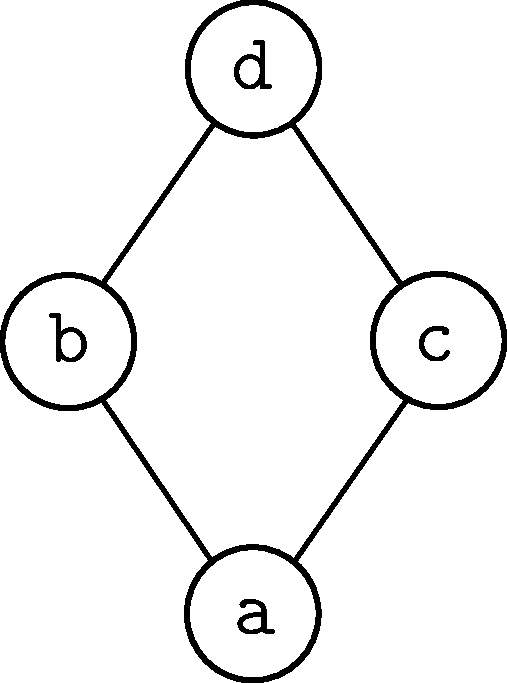
\includegraphics[width=.18\textwidth]{multi-inheritance.pdf}
\end{center}
\caption{\label{fig:multiple_paths_to_a_superclass}到同一基类的多条路径}
\end{figure}

如果需要实现继承系统的基本理念,我们就绝不能在检查一个对象的子类之
前,提前检查该对象。在本例中,正确的搜索顺序应该是~\texttt{a}、\texttt{b}、
\texttt{c}、\texttt{d}。那怎么样才能保证搜索的顺序是先尝试子孙再祖先呢?
最简单的办法是构造一个列表,列表由原始对象的所有祖先构成,然后对列表排序,
让列表中没有一个对象出现在它的子孙之前,最后再依次查看每个元素。

\texttt{get-ancestors} 采用了这种策略,它会返回一个按照上面规则排序的列
表,列表中的元素是对象和它的祖先们。\note{352}为了避免在排序时把同一层
次的祖先顺序打乱,\texttt{get-ancestors} 使用的是~\texttt{stable-sort}\index{stable-sort@\texttt{stable-sort}}\index{sorting|seealso {stable-sort@\texttt{stable-sort}}}
而非~\texttt{sort}\index{sort@\texttt{sort}}。一旦排序完毕,\texttt{rget} 只要找到第一个具有期望
属性的对象就可以了。(\utility~\texttt{some2} 是~\texttt{some} 的一个修
改版,它能适用于~\texttt{gethash} 这类用第二个返回值表示成功或失败的函数。)

对象的祖先列表中元素的顺序是先从最具体的开始,最后到最一般的类型。如
果~\texttt{orange} 是~\texttt{citrus} 的子类型,后者又
是~\texttt{fruit} 的子类型,那么列表的顺序就会像这样:\texttt{(orange
  citrus fruit)}。

% pp252
倘若有个对象,它具有多个父类,那么这些前辈的座次会是从左到右排列的。也就是
,如果我们说
\begin{lstlisting}
(setf (gethash 'parents x) (list y z))
\end{lstlisting}
那么当我们在搜索一个继承得来的属性时,\texttt{y} 就会优先于~\texttt{z}
被考虑。举个例子,我们可以说爱国的无赖\index{scoundrels, patriotic}首先是一个无赖,然后才是爱国者:
\begin{lstlisting}
> (setq scoundrel (make-hash-table)
        patriot (make-hash-table)
        patriotic-scoundrel (make-hash-table))
#<Hash-Table C4219E>
> (setf (gethash 'serves scoundrel) 'self
        (gethash 'serves patriot)   'country 
        (gethash 'parents patriotic-scoundrel)
                 (list scoundrel patriot))
(#<Hash-Table C41C7E> #<Hash-Table C41F0E>)
> (rget patriotic-scoundrel 'serves)
SELF
T
\end{lstlisting}

现在让我们对这个简陋的系统加以改进。可以从对象创建函数着手。这个
函数将会在新建对象时,构造一个该对象祖先的列表。虽然当前的版本是在进行
查询的时候构造这种表的,但是我们没有理由不把这件事情提前完成。
图~\ref{fig:a_function_to_create_objects} 中定义了一个名为~\texttt{obj} 的函数,这个函数被用于
生成新的对象,对象的祖先列表被保存在对象本身里。为了用上保存的祖先列
表,我们同时重新定义了~\texttt{rget}。
\begin{figure}
\begin{lstlisting}
(defun obj (&rest parents)
  (let ((obj (make-hash-table)))
    (setf (gethash 'parents obj) parents)
    (ancestors obj)
    obj))

(defun ancestors (obj)
  (or (gethash 'ancestors obj)
      (setf (gethash 'ancestors obj) (get-ancestors obj))))

(defun rget (obj prop)
  (some2 #'(lambda (a) (gethash prop a))
         (ancestors obj)))
\end{lstlisting}
\index{rget@\texttt{rget}}
\caption{\label{fig:a_function_to_create_objects}用来新建对象的函数}
\index{superclasses!precedence of!sketch of}
\end{figure}

另一个可以改进的地方是消息调用的语法。\texttt{tell} 本身是多余的东西,
并且由于它的原因,动词被排到了第二位。这意味着我们的程序读起来不再
像是熟悉的~Lisp 前缀表达式了\index{message-passing 消息传递!vs. Lisp syntax 对阵~Lisp 语法}:
\begin{lstlisting}
(tell (tell obj 'find-owner) 'find-owner)
\end{lstlisting}

\begin{figure}
\begin{lstlisting}
(defmacro defprop (name &optional meth?)
  `(progn
     (defun ,name (obj &rest args)
       ,(if meth?
            `(run-methods obj ',name args)
            `(rget obj ',name)))
     (defsetf ,name (obj) (val)
       `(setf (gethash ',',name ,obj) ,val))))

(defun run-methods (obj name args)
  (let ((meth (rget obj name)))
    (if meth
        (apply meth obj args)
      (error "No ~A method for ~A." name obj))))
\end{lstlisting}
\index{defprop@\texttt{defprop}}
\caption{\label{fig:functinoal_syntax}函数式的语法}
\end{figure}
我们可以通过把每个属性定义成函数来去掉~\texttt{tell} 这种语法,如
图~\ref{fig:functinoal_syntax} 所示。可选参数~\texttt{meth?} 的值如果是真的话,那表示这
个属性应该被当作方法来处理,否则它应该被当成一个~slot,并径直返
回~\texttt{rget} 所取到的值。一旦我们把这两种属性中任一种,像这样定义好
了:
\begin{lstlisting}
(defprop find-owner t)
\end{lstlisting}
我们就可以用函数调用的方式来引用它,同时代码读起来又有~Lisp 的样子了:
\begin{lstlisting}
(find-owner (find-owner obj))
\end{lstlisting}
现在,原先的例子也变得更有可读性了:
\begin{lstlisting}
> (progn
    (setq scoundrel (obj))
    (setq patriot (obj))
    (setq patriotic-scoundrel (obj scoundrel patriot))
    (defprop serves)
    (setf (serves scoundrel) 'self)
    (setf (serves patriot) 'country)
    (serves patriotic-scoundrel))
SELF
T
\end{lstlisting}

在当前的实现里,对象中每个名字最多对应一个方法。这个方法要么是对象
自己的,要么是通过继承得来的。要是能在这个问题上有更多的灵活性,允许
把本地的方法和继承来的方法组合起来,那肯定会方便很多。比如说,
我们会希望某个对象的~\texttt{move} 方法沿用其父类的~\texttt{move} 
方法,但是除此之外还要在调用之前或者之后运行一些其它的代码。

为了让这个设想变成现实,我们将修改程序,加上~before、after 和~around 方
法。before 方法让我们能吩咐程序,``先别急,把这事做完再说''。这些方法会
在该方法中其余部分运行前,作为前奏,被先行调用。after 方法让我们可以要求程序
说,``还有,把这事也给办了''。而这些方法会作为收场在最后调用。在两者之间,
我们会执行曾经自己就是整个方法的函数,现在被称为\emph{主方法}~(primary method)。
它的返回值将被作为整个方法的返回值,即使~after 方法在其后调用。

before 和~after 方法让我们能用新的行为把主方法包起来。around 方法则以
一种更奇妙的方法实现了这个功能。如果存在~around 方法,那么被调用的就不
再是主方法,\emph{而是}~around 方法。并且,around 方法有办法调用主方
法~(用~\verb|call-next|,该函数在图~\ref{fig:defining_methods} 中提供),至于调
不调则是它的自由。
\begin{figure}
\begin{lstlisting}
(defstruct meth around before primary after)

(defmacro meth- (field obj)
  (let ((gobj (gensym)))
    '(let ((,gobj ,obj))
       (and (meth-p ,gobj)
            (,(symb 'meth- field) ,gobj)))))

(defun run-methods (obj name args)
  (let ((pri (rget obj name :primary)))
    (if pri
        (let ((ar (rget obj name :around)))
          (if ar
              (apply ar obj args)
              (run-core-methods obj name args pri)))
        (error "No primary ~A method for ~A." name obj))))

(defun run-core-methods (obj name args &optional pri)
  (multiple-value-prog1
   (progn (run-befores obj name args)
          (apply (or pri (rget obj name :primary))
                 obj args))
   (run-afters obj name args)))

(defun rget (obj prop &optional meth (skip 0))
  (some2 #'(lambda (a)
             (multiple-value-bind (val win) (gethash prop a)
               (if win
                   (case meth (:around (meth- around val))
                              (:primary (meth- primary val))
                              (t (values val win))))))
         (nthcdr skip (ancestors obj))))
\end{lstlisting}
\index{methods 方法!auxiliary 辅助!sketch of}
\caption{\label{fig:auxiliary_methods}辅助的方法}
\end{figure}

\begin{figure}
\begin{lstlisting}
(defun run-befores (obj prop args)
  (dolist (a (ancestors obj))
    (let ((bm (meth- before (gethash prop a))))
      (if bm (apply bm obj args)))))

(defun run-afters (obj prop args)
  (labels ((rec (lst)
                (when lst
                  (rec (cdr lst))
                  (let ((am (meth- after
                                   (gethash prop (car lst)))))
                    (if am (apply am (car lst) args))))))
    (rec (ancestors obj))))
\end{lstlisting}
\index{methods 方法!before-!sketch of}
\index{methods 方法!after-!sketch of}
\caption{\label{fig:auxiliary_methods_cont}辅助的方法~(续)}
\end{figure}
如图~\ref{fig:auxiliary_methods} 和图~\ref{fig:auxiliary_methods_cont}
所示,为了让这些辅助的方法生效,我们
对~\verb|run-methods| 和~\verb|rget| 加以了改进。在之前的版本里,当
我们调用对象的某个方法时,运行的仅是一个函数:即最匹配的那个主函数。我
们将会运行搜索祖先列表时找到的第一个方法。加上辅助方法的支持,调用的顺
序将变成这样:
\begin{enumerate}
  \item 倘若有的话,先是最匹配的~around 方法
  \item 否则的话,依次是:
  \begin{enumerate}
    \item 所有的~before 方法,从最匹配的到最不匹配的。
    \item 最匹配的主方法~(这是我们以前会调用的)。
    \item 所有的~after 方法,从最不匹配的到最匹配的。
  \end{enumerate}
\end{enumerate}

同时也注意到,方法不再作为单个的函数出现,它成了有四个成员的结构。
现在要定义一个~(主) 方法,不能再像这样说了:
\begin{lstlisting}
(setf (gethash 'move obj) #'(lambda ...))
\end{lstlisting}
我们改口说:
\begin{lstlisting}
(setf (meth-primary (gethash 'move obj)) #'(lambda ...))
\end{lstlisting}
基于上面、还有其它一些原因,我们下一步将会定义一个宏,让它帮我们定
义方法。
\begin{figure}
\begin{lstlisting}
(defmacro defmeth ((name &optional (type :primary))
                   obj parms &body body)
  (let ((gobj (gensym)))
    `(let ((,gobj ,obj))
       (defprop ,name t)
       (unless (meth-p (gethash ',name ,gobj))
         (setf (gethash ',name ,gobj) (make-meth)))
       (setf (,(symb 'meth- type) (gethash ',name ,gobj))
             ,(build-meth name type gobj parms body)))))

(defun build-meth (name type gobj parms body)
  (let ((gargs (gensym)))
    `#'(lambda (&rest ,gargs)
         (labels
             ((call-next ()
                ,(if (or (eq type :primary)
                         (eq type :around))
                     `(cnm ,gobj ',name (cdr ,gargs) ,type)
                     '(error "Illegal call-next.")))
              (next-p ()
                ,(case type
                   (:around
                    `(or (rget ,gobj ',name :around 1)
                         (rget ,gobj ',name :primary)))
                   (:primary
                    `(rget ,gobj ',name :primary 1))
                   (t nil))))
           (apply #'(lambda ,parms ,@body) ,gargs)))))

(defun cnm (obj name args type)
  (case type
    (:around (let ((ar (rget obj name :around 1)))
               (if ar
                   (apply ar obj args)
                   (run-core-methods obj name args))))
    (:primary (let ((pri (rget obj name :primary 1)))
                (if pri
                    (apply pri obj args)
                    (error "No next method."))))))
\end{lstlisting}
\index{methods 方法!around-!sketch of}
\index{next-method-p@\texttt{next-method-p}!sketch of}
\index{call-next-method@\texttt{call-next-method}!sketch of}
\caption{\label{fig:defining_methods}定义方法}
\end{figure}

图~\ref{fig:defining_methods} 定义的就是这样的一个宏。代码中有很大篇幅被用来实现两
个函数,这两个函数让方法能引用其它的方法。around 和主方法可以使
用~\texttt{call-next} 来调用\emph{下一个方法},所谓下一个方法,指的是倘
若当前方法不存在,就会被调用的方法。举个例子,如果当前运行的方法是唯一
的一个~around 方法,那么下一个方法就是常见的由~before 方法、最匹配的主
方法和~after 方法三者合体而成的夹心饼干。在最匹配的主方法里,下一个方法
则会是第二匹配的主方法。由于~\texttt{call-next} 的行为取决于它被调用的
地方,因此~\texttt{call-next} 绝对不会用一个~\texttt{defun} 来在全局定
义,不过它可以在每个由~\texttt{defmeth} 定义的方法里局部定义。

around 方法或者主方法可以用~\texttt{next-p} 来获知下一个方法是否存在。
如果当前的方法是个主方法,而且主方法所属的对象是没有父类的,那么就不会
有下一个方法。由于当没有下个方法时,~\texttt{call-next} 会报错,因此应
该经常调用~\texttt{next-p} 试试深浅。像~\texttt{call-next},
\texttt{next-p} 也是在方法里面单独地局部定义的。

下面将介绍新宏~\texttt{defmeth} 的使用方法。如果我们只是希望定
义~\texttt{rectangle} 对象的~\texttt{area} 方法,我们会说
\begin{lstlisting}
(setq rectangle (obj))
(defprop height)
(defprop width)
(defmeth (area) rectangle (r)
  (* (height r) (width r)))
\end{lstlisting}

现在,一个~\texttt{rectangle} 实例的面积就会由类型中对应方法计算得出:
\begin{lstlisting}
> (let ((myrec (obj rectangle)))
    (setf (height myrec) 2
          (width myrec)  3)
    (area myrec))
6
\end{lstlisting}
这里有个复杂一些的例子,假设我们为~\texttt{filesystem} 对象定义了一
个~\texttt{backup} 方法:
\begin{lstlisting}
(setq filesystem (obj))
(defmeth (backup :before) filesystem (fs)
  (format t "Remember to mount the tape.~%"))
(defmeth (backup) filesystem (fs)
  (format t "Oops, deleted all your files.~%")
  'done)
(defmeth (backup :after) filesystem (fs)
  (format t "Well, that was easy.~%"))
\end{lstlisting}
正常的调用次序如下:
\begin{lstlisting}
> (backup (obj filesystem))
Remember to mount the tape.
Oops, deleted all your files.
Well, that was easy.
DONE
\end{lstlisting}
接下来,我们想要知道备份一次会花费多少时间,所以可以定义下面的~around 方
法:
\begin{lstlisting}
(defmeth (backup :around) filesystem (fs)
  (time (call-next)))
\end{lstlisting}
现在只要调用~\texttt{filesystem} 子类的~\texttt{backup}~(除非有更匹配
的~around 方法介入),那么我们的~around 方法就会执行。它会运行平常时候
在~\texttt{backup} 里运行的那些代码,不同之处是把它们放到了一
个~\texttt{time}\index{time@\texttt{time}} 的调用里执行。\texttt{time} 的返回值则会被作
为~\texttt{backup} 方法调用的值返回。
\begin{lstlisting}
> (backup (obj filesystem))
Remember to mount the tape.
Oops, deleted all your files.
Well, that was easy.
Elapsed Time = .01 seconds
DONE
\end{lstlisting}
一旦知道了备份操作需要的时间,我们就会想要去掉这个~around 方
法。调用~\texttt{undefmeth} 可达到这个目的~(如图~\ref{fig:removing_methods}),
它的参数和~\texttt{defmeth} 的前两个参数相同:
\begin{lstlisting}
(undefmeth (backup :around) filesystem)
\end{lstlisting}

\begin{figure}
\begin{lstlisting}
(defmacro undefmeth ((name &optional (type :primary)) obj)
  `(setf (,(symb 'meth- type) (gethash ',name ,obj))
         nil))
\end{lstlisting}
\caption{\label{fig:removing_methods}去掉方法}
\index{methods 方法!removing 删除!sketch of}
\end{figure}

另外一个我们可能需要修改的是对象的父类列表。但是进行了这种修改之后,我
们还应该相应地更新该对象以及其所有子类的的祖先列表。到目前为止,还没有
办法从对象那里获知它的子类信息,所以我们必须另加一个~\texttt{children}
属性。

\begin{figure}
\begin{lstlisting}
(defmacro children (obj)
  `(gethash 'children ,obj))

(defun parents (obj)
  (gethash 'parents obj))

(defun set-parents (obj pars)
  (dolist (p (parents obj))
    (setf (children p)
          (delete obj (children p))))
  (setf (gethash 'parents obj) pars)
  (dolist (p pars)
    (pushnew obj (children p)))
  (maphier #'(lambda (obj)
               (setf (gethash 'ancestors obj)
                     (get-ancestors obj)))
             obj)
  pars)

(defsetf parents set-parents)

(defun maphier (fn obj)
  (funcall fn obj)
  (dolist (c (children obj))
    (maphier fn c)))

(defun obj (&rest parents)
  (let ((obj (make-hash-table)))
    (setf (parents obj) parents)
    obj))
\end{lstlisting}
\caption{\label{fig:maintaining_parent_n_child_links}维护父类和子类的联系}
\end{figure}
图~\ref{fig:maintaining_parent_n_child_links} 中的代码被用来操作对象的
父类和子类。这里不再用~\texttt{gethash} 来获得父类和子类信息,而是分别
改用操作符~\texttt{parents} 和~\texttt{children}。其中后者是个宏,因而
它对于~\texttt{setf} 是透明的。前者是一个函数,它的逆操作
被~\texttt{defsetf} 定义为~\texttt{set-parents},这个函数包揽了所有的相
关工作,让新的双向链接系统能保持其一致性。

为了更新一颗子树里所有对象的祖先,\texttt{set-parents} 调用了
~\texttt{maphier},这个函数的作用相当于继承树里的
~\texttt{mapc}。\texttt{mapc} 对列表里每个元素运行一个函数,同样
的,\texttt{maphier} 也会对对象和它所有的后代应用指定的函数。除非这些节点构成
没有公共子节点的树,否则有的对象会被传入这个函数一次以上。在这里,这不会导致问题,
因为调用多次~\texttt{get-ancestors} 和调用一次的效果是相同的。

现在,要修改继承层次结构的话,我们只要在对象的~\texttt{parents} 上调
用~\texttt{setf} 就可以了:
\begin{lstlisting}
> (progn (pop (parents patriotic-scoundrel))
         (serves patriotic-scoundrel))
COUNTRY
T
\end{lstlisting}
当这个层次结构被修改的时候,受到影响的子孙列表和祖先列表会同时自动地更
新。(\texttt{children} 本不是让人直接修改的,但是这也不是不可以。只要我
们定义一个和~\texttt{set-parents} 对应的~\texttt{set-children} 就可以
了。) 为了配合新代码,我们在图~\ref{fig:maintaining_parent_n_child_links} 
的最后重新定义了~\verb|obj| 函数。

这次我们要开发一个新的手段来组合方法,作为对这个系统的最后一项改进。现
在,会被调用的唯一主方法将是最匹配的那个~(虽然它可以用~\texttt{call-next} 
来调用其它的主方法)。要是我们希望能把对象所有祖先的主方法的结果组合起来呢?
比如说,假设~\texttt{my-orange} 是~\texttt{orange} 的子类,而
~\texttt{orange} 又是~\texttt{citrus} 的子类。如果~\texttt{props} 
方法用在~\texttt{citrus} 上的返回值是~\texttt{(round acidic)},
相应的,\texttt{orange} 的返回值是~\texttt{(orange sweet)},
\texttt{my-orange} 的结果是~\texttt{(dented)}。要是能让
~\texttt{(props my-orange)} 能返回这些值的\emph{并集}就好办多了:
\texttt{(dented orange sweet round acidic)}。

\begin{figure}
\begin{lstlisting}
(defmacro defcomb (name op)
  `(progn
     (defprop ,name t)
     (setf (get ',name 'mcombine)
           ,(case op
              (:standard nil)
              (:progn '#'(lambda (&rest args)
                           (car (last args))))
              (t op)))))

(defun run-core-methods (obj name args &optional pri)
  (let ((comb (get name 'mcombine)))
    (if comb
        (if (symbolp comb)
            (funcall (case comb (:and #'comb-and)
                           (:or #'comb-or))
                     obj name args (ancestors obj))
          (comb-normal comb obj name args))
      (multiple-value-prog1
       (progn (run-befores obj name args)
              (apply (or pri (rget obj name :primary))
                     obj args))
       (run-afters obj name args)))))

(defun comb-normal (comb obj name args)
  (apply comb
         (mapcan #'(lambda (a)
                     (let* ((pm (meth- primary
                                       (gethash name a)))
                            (val (if pm
                                     (apply pm obj args))))
                       (if val (list val))))
                   (ancestors obj))))
\end{lstlisting}
\index{method combination 方法的组合!progn@\texttt{progn}!sketch of}
\index{method combination 方法的组合!operator!sketch of}
\caption{\label{fig:method_combination}方法的组合}
\end{figure}

假如能让方法对所有主方法的返回值应用某个函数,而不是仅仅返回最匹配
的那个主函数的返回值,那就能解决这个问题了。图~\ref{fig:method_combination} 中
定义有一个宏,这个宏让我们能指定方法的组合手段,图中还定义了新版本的
~\texttt{run-core-methods},它允许我们把方法组合在一起使用。
我们用~\texttt{defcomb} 定义方法的组合形式,它把方法名作为第一个参
数,第二个参数描述了期望的组合方式。通常,这第二个参数应该是一个函数。
不过,它也可以是~\texttt{:progn}、\texttt{:and}、\texttt{:or} 
和~\texttt{:standard}中的一个。如果使用前三个,系统就会用相应的操作
符来组合主方法,用~\texttt{:standard} 的话,就表示我们想用以前的办法
来执行方法。

图~\ref{fig:method_combination} 中的核心函数是新
的~\texttt{run-core-methods}。如果被调用的方法没有名
为~\texttt{mcombine} 的属性,那么一切如常。否则,\texttt{mcombine} 应该
是个函数~(比如~\texttt{+}),或是个关键字~(比如~\texttt{:or})。前面一
种情况,所有主方法返回值构成的列表会被送进这个函数。\footnote{如果代码
  写得更讲究一些,可以考虑用~\texttt{reduce}\index{reduce@\texttt{reduce}},这样可以避免手
  动~cons。}如果是后者的情况,我们会用和这个关键字对应的函数对主方法一
一进行操作。
\begin{figure}
\begin{lstlisting}
(defun comb-and (obj name args ancs &optional (last t))
  (if (null ancs)
      last
    (let ((pm (meth- primary (gethash name (car ancs)))))
      (if pm
          (let ((new (apply pm obj args)))
            (and new
                 (comb-and obj name args (cdr ancs) new)))
        (comb-and obj name args (cdr ancs) last)))))

(defun comb-or (obj name args ancs)
  (and ancs
       (let ((pm (meth- primary (gethash name (car ancs)))))
         (or (and pm (apply pm obj args))
             (comb-or obj name args (cdr ancs))))))
\end{lstlisting}
\index{method combination 方法的组合!and@\texttt{and}!sketch of}
\index{method combination 方法的组合!or@\texttt{or}!sketch of}
\caption{\label{fig:method_combination_cont}方法的组合~(续)}
\end{figure}

如图~\ref{fig:method_combination_cont} 所示,\texttt{and} 和~\texttt{or}
这两个操作符必须要特殊处理。它们被特殊对待的原因不是因为它们是~special form,
而是因为它们的短路~(short-circuit) 求值方式:
\begin{lstlisting}
> (or 1 (princ "wahoo"))
1
\end{lstlisting}
这里,什么都不会被打印出来,因为~\texttt{or} 一看到非~nil 的参数就会立
即返回。与之类似,如果有一个更匹配的方法返回真的话,那么剩下的
用~\texttt{or} 组合的主方法将不会被调用。为了实
现~\texttt{and} 和~\texttt{or} 的这种短路求值,我们用了两个专门的函
数:\texttt{comb-and} 和~\texttt{comb-or}。

为了实现我们之前的例子,可以这样写:
\begin{lstlisting}
(setq citrus (obj))
(setq orange (obj citrus))
(setq my-orange (obj orange))

(defmeth (props) citrus (c) '(round acidic))
(defmeth (props) orange (c) '(orange sweet))
(defmeth (props) my-orange (m) '(dented))

(defcomb props #'(lambda (&rest args) (reduce #'union args)))
\end{lstlisting}
这样定义之后,\texttt{props} 就能返回所有主方法返回值的并集了:
\footnote{由于~\texttt{props} 里用的组合函数是~\texttt{union},因此
列表里的元素不一定会按照原来的顺序排列\index{union@\texttt{union}!unspecified order of result 结果的顺序不确定}。}
%% xxx, the generated entry in idx file always looks like 
%% \indexentry{union@\texttt  {union}!unspecified order of result 结果的顺序不确定|hyperpage}
%% so be it

\begin{lstlisting}
> (props my-orange)
(DENTED ORANGE SWEET ROUND ACIDIC)
\end{lstlisting}

这个例子恰巧显示了一个只有在~Lisp 里用面向对象编程才会面临的选择:
是把信息保存在~slot 里,还是保存在方法里。

以后,如果想要~\texttt{props} 方法恢复到缺省的行为,只要把方法的组合方式改回标准模式~(standard) 即可:
\begin{lstlisting}
> (defcomb props :standard)
NIL
> (props my-orange)
(DENTED)
\end{lstlisting}
要注意,before 和~after 方法只是在标准的组合模式下才会有效。而~around
方法会像以前那样工作。

本节中展示的程序只是作为一个演示模型,而不是想以它为基础,进行面向对象
编程。写这个模型的着眼点是简洁而非效率。不管如何,这至少是一个可以工作
的模型,因此也可以被用在试验性质的开发和原型开发中。如果你有意这样用它
的话,有一个小改动可以让它的效率有相当的改进:如果对象只有一个父类的话,
就不要计算或者保存它的祖先列表。

\section{类和实例}
\label{sec:classes_and_instances}

上一节中写了一个尽可能短小的程序来重新实现~CLOS。理解它为我们进而理
解~CLOS 铺平了道路。在下面几节中,我们会仔细考察~CLOS\index{CLOS@\textsc{clos}} 本身。

在我们的这个简单实现里,没有把类和实例作语法上的区分,也没有把
~slot 和方法分开。在~CLOS 里,我们用~\texttt{defclass}\index{defclass@\texttt{defclass}} 定义类\index{classes 类!defining 定义},同时
把各 slot 组成列表一并声明\index{slots!declaring 声明}:
\begin{lstlisting}
(defclass circle ()
  (radius center))
\end{lstlisting}
这个表达式的意思是,\texttt{circle} 类没有父类,但是有两个~slot:
\texttt{radius} 和~\texttt{center}。我们用下面的语句可以新建一个
~circle 类的实例\index{instances 实例}:
\begin{lstlisting}
(make-instance 'circle)
\end{lstlisting}
\index{make-instance@\texttt{make-instance}}
不幸的是,我们还没有定义读取~\texttt{circle} 中~slot 的方式,因此我们创
建的任何实例都只是个摆设。为了访问特定的~slot,我们需要为它定义一个
访问~(accessor) 函数\index{slots!accessor functions for}:
\begin{lstlisting}
(defclass circle ()
  ((radius :accessor circle-radius)
   (center :accessor circle-center)))
\end{lstlisting}
\index{accessor@\texttt{:accessor}}
现在,如果我们建立了一个~circle 的实例,就可以用~\texttt{setf} 和与
之对应的访问函数来设置它的~\texttt{radius} 和~\texttt{center} slot:
\begin{lstlisting}
> (setf (circle-radius (make-instance 'circle)) 2)
2
\end{lstlisting}
如果像下面那样定义~slot,那么我们也可以在~\texttt{make-instance} 里直接
完成这种初始化的工作\index{slots!initializing}:
\begin{lstlisting}
(defclass circle ()
  ((radius :accessor circle-radius :initarg :radius)
   (center :accessor circle-center :initarg :center)))
\end{lstlisting}
在~slot 定义中出现的~\texttt{:initarg}\index{initarg@\texttt{:initarg}} 关键字表示:接下来的实参将要
在~\texttt{make-instance} 中成为一个关键字形参。这个关键字实参的值
将会被作为该~slot 的初始值:
\begin{lstlisting}
> (circle-radius (make-instance 'circle
                   :radius 2
                   :center '(0 . 0)))
2
\end{lstlisting}

使用\texttt{:initform}\index{initform@\texttt{:initform}},我们也可以定义一些~slot,让它们能初始化自己。
\texttt{shape} 类中的~\texttt{visible}
\begin{lstlisting}
(defclass shape ()
  ((color   :accessor shape-color   :initarg :color)
   (visible :accessor shape-visible :initarg :visible
            :initform t)))
\end{lstlisting}
会缺省地被设置成~\texttt{t}:
\begin{lstlisting}
> (shape-visible (make-instance 'shape))
T
\end{lstlisting}
如果一个~slot 同时具有~initarg 和~initform,那么当~initarg 被指定的时
候,它享有优先权:
\begin{lstlisting}
> (shape-visible (make-instance 'shape :visible nil))
NIL
\end{lstlisting}

slot 会被实例和子类继承\index{inheritance!of slots}下来。如果一个类有多个父类\index{inheritance!multiple},那么它会继承得到这些
父类~slot 的并集。因此,如果我们把~\texttt{screen-circle} 类同时定义
成~\texttt{circle} 和~\texttt{shape} 两个类的子类,
\begin{lstlisting}
(defclass screen-circle (circle shape)
  nil)
\end{lstlisting}
那么~\texttt{screen-circle} 会具有四个~slot,每个父类继承两个~slot。注意
到,一个类并不一定要自己新建一些新的~slot,\texttt{screen-circle} 的意
义就在于提供了一个可以实例化的类型,它同时继承自~\texttt{circle} 和
~\texttt{shape}。

以前可以用在~\texttt{circle} 和~\texttt{shape} 实例的那些访问函数
和~initarg 会对~\texttt{screen-circle} 类型的实例继续生效:
\begin{lstlisting}
> (shape-color (make-instance 'screen-circle
                              :color 'red :radius 3))
RED
\end{lstlisting}
如果在~\texttt{defclass} 里给~\texttt{color} 指定一个~initform,我们就
可以让所有的~\texttt{screen-circle} 的对应~slot 都有个缺省值:
\begin{lstlisting}
(defclass screen-circle (circle shape)
  ((color :initform 'purple)))
\end{lstlisting}
这样,\texttt{screen-circle} 类型的实例在缺省情况下就会是紫色的了:
\begin{lstlisting}
> (shape-color (make-instance 'screen-circle))
PURPLE
\end{lstlisting}
不过我们还是可以通过显式地指定一个~\texttt{:color} initarg,来把这个~slot 初始化
成其他颜色。

在我们之前实现的简装版面向对象编程框架里,实例的值可以直接从父类
的~slot 继承得到。在~CLOS 中,实例包含~slot 的方式却和类不一样。我们通
过在父类里定义~initform 来为实例定义可被继承的缺省值。在某种程度上,这
样处理更有灵活性。因为~initform 不仅可以是一个常量,它还可以是一个每次
都返回不同值的表达式:
\begin{lstlisting}
(defclass random-dot ()
  ((x :accessor dot-x :initform (random 100))
   (y :accessor dot-y :initform (random 100))))
\end{lstlisting}
每创建一个~\texttt{random-dot} 实例,它在~x 和~y 轴上的坐标都会是
从~0 到~99 之间的一个随机整数:
\begin{lstlisting}
> (mapcar #'(lambda (name)
               (let ((rd (make-instance 'random-dot)))
                 (list name (dot-x rd) (dot-y rd))))
          '(first second third))
((FIRST 25 8) (SECOND 26 15) (THIRD 75 59))
\end{lstlisting}

在我们的简装版实现里,我们对两种~slot 不加区别:一种是实例自己具有
的~slot,这种~slot 实例和实例之间可以不同;另一种~slot 应该是在整个类里
面都相同的。在~CLOS 中,我们可以指定某些~slot 是\emph{共享的},换句话
说,就是让这些~slot 的值在每个实例里都是相同的。为了达到这个效果,我们可以
把~slot 声明成~\texttt{:allocation :class} 的。(另一个选项
是~\texttt{:allocation :instance}。不过由于这是缺省的设置,因此就没有必
要再显式地指定了。) 比如说,如果所有的猫头鹰都是夜间生活的动物,那么我
们可以让~\texttt{nocturnal} 这个~slot 作为~\texttt{owl} 类的共
享~slot,同时让它的初始值为~\texttt{t}:
\begin{lstlisting}
(defclass owl ()
  ((nocturnal :accessor owl-nocturnal
              :initform t
              :allocation :class)))
\end{lstlisting}
\index{allocation@\texttt{:allocation}}
现在,所有的~\texttt{owl} 实例都会继承这个~slot 了:
\begin{lstlisting}
> (owl-nocturnal (make-instance 'owl))
T
\end{lstlisting}
如果我们改动了这个~slot 的``局部''值,那么我们实际上修改的是保存在这个
类里面的值:
\begin{lstlisting}
> (setf (owl-nocturnal (make-instance 'owl)) 'maybe)
MAYBE
> (owl-nocturnal (make-instance 'owl))
MAYBE
\end{lstlisting}

这种机制或许会造成一些困扰,所以我们可能会希望让这个~slot 成为只读的\index{slots!read-only}。
在我们为一个~slot 定义访问函数的同时,也是在为这个~slot 的值定义一个读
和写的方法。如果我们需要让这个值可读,但是不可写,那么我们可以给这
个~slot 仅仅设置一个~reader 函数\index{reader@\texttt{:reader}},而不是全功能的访问函数:
\begin{lstlisting}
(defclass owl ()
  ((nocturnal :reader owl-nocturnal
              :initform t
              :allocation :class)))
\end{lstlisting}
现在如果尝试修改~\texttt{owl} 实例的~\texttt{nocturnal} slot 的话,就会
产生一个错误:
\begin{lstlisting}
> (setf (owl-nocturnal (make-instance 'owl)) nil)
>> Error: The function (SETF OWL-NOCTURNAL) is undefined.
\end{lstlisting}

\section{方法}
\label{sec:methods}

在我们的简装版实现中,强调了这样一个思想,即在具有词法作用域的语言里,其~slot 和方法
间是有其相似性的\index{methods 方法!isomorphic to slots 和~slot 间的相似性}\index{slots!isomorphic to methods 和方法间的相似性}。在实现的时候,保存和继承主方法的方式和对~slot 值的处理方
式没有什么不同。slot 和方法区别只在于:把一个名字定义成~slot,是通过
\begin{lstlisting}
(defprop area)
\end{lstlisting}
把~\texttt{area} 作为一个函数实现的,这个函数得到并返回一个值。而把这个
名字定义成一个方法,则是通过
\begin{lstlisting}
(defprop area t)
\end{lstlisting}
把~\texttt{area} 实现成一个函数,这个函数在得到值之后,会~funcall 这个
值,同时把函数的参数传给它。

在~CLOS 中,实现这个功能的单元仍然被称为``方法'',同时也可以定义这些方
法,让它们看上去就像类的属性一样。\index{methods 方法!of classes 类的}这里,我们为~\texttt{circle} 类定义一
个名为~\texttt{area} 的方法:
\begin{lstlisting}
(defmethod area ((c circle))
  (* pi (expt (circle-radius c) 2)))
\end{lstlisting}
这个方法的参数列表表示,这是个接受一个参数的函数,参数应该
是~\texttt{circle} 类型的实例。

和简单实现里一样,我们像调用一个函数那样调用这个方法:
\begin{lstlisting}
> (area (make-instance 'circle :radius 1))
3.14...
\end{lstlisting}
我们同样可以让方法接受更多的参数:
\begin{lstlisting}
(defmethod move ((c circle) dx dy)
  (incf (car (circle-center c)) dx)
  (incf (cdr (circle-center c)) dy)
  (circle-center c))
\end{lstlisting}
如果我们对一个~\texttt{circle} 的实例调用这个方法,\texttt{circle} 实例的中心会移动~$\langle$\texttt{dx},\texttt{dy}$\rangle$:
\begin{lstlisting}
> (move (make-instance 'circle :center '(1 . 1)) 2 3)
(3 . 4)
\end{lstlisting}
方法的返回值表明了圆形的新位置。

和我们的简装版实现一样,如果一个实例对应的类及其父类有个方法,那么调用
这个方法会使最匹配的方法被调用。因此,如果~\texttt{unit-circle} 是
~\texttt{circle} 的子类,同时具有如下所示的~\texttt{area} 方法:
\begin{lstlisting}
(defmethod area ((c unit-circle)) pi)
\end{lstlisting}
那么当我们对一个~\texttt{unit-circle} 的实例调用~\texttt{area} 方法的时
候,将被调用的不是更一般的那个方法,而是在上面定义~\texttt{area}。

当一个类有多个父类时,它们的优先级\index{superclasses!precedence of}从左到右依次降低。
\texttt{patriotic-scoundrel} 类的定义如下:
\begin{lstlisting}
(defclass scoundrel nil nil)
(defclass patriot nil nil)
(defclass patriotic-scoundrel (scoundrel patriot) nil)
\end{lstlisting}
我们认为爱国的无赖,他首先是一个无赖,然后才是一个爱国者。当两个父类
都有合适的方法时,
\begin{lstlisting}
(defmethod self-or-country? ((s scoundrel))
  'self)

(defmethod self-or-country? ((p patriot))
  'country)
\end{lstlisting}
\texttt{scoundrel} 类的方法会这样被执行:
\begin{lstlisting}
> (self-or-country? (make-instance 'patriotic-scoundrel))
SELF
\end{lstlisting}

到目前为止,所以的例子都让人觉得~CLOS 中的方法只针对某一个类。实际
上,CLOS 中的方法是更为通用的一个概念。在~\texttt{move} 方法的参数列表
中,我们称~\verb|(c circle)| 为\emph{特化}~(specialized)\index{methods 方法!specialization of 的特化} 参
数,它表示,如果~\texttt{move} 的第一个参数是~\texttt{circle} 类的一个
实例的话,就适用这个方法。对于~CLOS 方法,\emph{不止一个参数可以被特化}。
下面的方法就有两个特化参数和一个可选的非特化参数:
\begin{lstlisting}
(defmethod combine ((ic ice-cream) (top topping)
                    &optional (where :here))
  (append (list (name ic) 'ice-cream)
          (list 'with (name top) 'topping)
          (list 'in 'a
                (case where
                  (:here 'glass)
                  (:to-go 'styrofoam))
                'dish)))
\end{lstlisting}
如果~\texttt{combine} 的前两个参数分别
是~\texttt{ice-cream}\index{ice-cream} 和~\texttt{topping} 的实例的话,上面定义的方法就
会被调用。如果我们定义几个最简单类以便构造实例
\begin{lstlisting}
(defclass stuff () ((name :accessor name :initarg :name)))
(defclass ice-cream (stuff) nil)
(defclass topping (stuff) nil)
\end{lstlisting}
那么我们就能定义并运行这个方法了:
\begin{lstlisting}
> (combine (make-instance 'ice-cream :name 'fig)
           (make-instance 'topping :name 'olive)
           :here)
(FIG ICE-CREAM WITH OLIVE TOPPING IN A GLASS DISH)
\end{lstlisting}

倘若方法特化了一个以上的参数,这时就没有办法再把方法当成类的属性了。我
们的~\texttt{combine} 方法是属于~\texttt{ice-cream} 类还是属
于~\texttt{topping} 类呢?在~CLOS 里,所谓``对象响应消息''的模型不复存
在。如果我们像下面那样调用函数,这种模型似乎还是顺理成章的:
\begin{lstlisting}
(tell obj 'move 2 3)
\end{lstlisting}
显而易见,在这里我们调用的是~\texttt{obj} 的~\texttt{move} 方法。
但是一旦我们废弃这种语法,而改用函数风格的等价操作:
\begin{lstlisting}
(move obj 2 3)
\end{lstlisting}
我们就需要定义~\texttt{move},让它能根据它的第一个参数~\emph{dispatch}\index{dispatching 分派} 操
作,即按照第一个参数的类型来调用适合的方法。

走出这一步,于是有个问题浮出了水面:为什么只能根据第一个参数来进
行~dispatch 呢?CLOS 的回答是:就是呀,为什么非得这样呢?在~CLOS 中,方法能够指定任意
个数的参数进行特化\index{methods 方法!specialization of 的特化!on types 针对类型},而且这并不限于用户自定义的类,Common
Lisp 类型\footnote{或者更准确地说,是~CLOS 定义的一系列形似类型的类,这
  些类的定义和~Common Lisp 的内建类型体系是平行对应的。}也一样可以,甚
至能针对单个的特定对象特化\index{types 类型!specialization on 特化}。下面是一个名为~\texttt{combine} 的方法,它被
用于字符串:
\begin{lstlisting}
(defmethod combine ((s1 string) (s2 string) &optional int?)
  (let ((str (concatenate 'string s1 s2)))
    (if int? (intern str) str)))
\end{lstlisting}
这不仅意味着方法不再是类的属性,而且还表明,我们可以根本不用定义类就能
使用方法了\index{methods 方法!without classes 脱离类的}。
\begin{lstlisting}
> (combine "I am not a " "cook.")
"I am not a cook."
\end{lstlisting}
下面,第二个参数将对符号~\texttt{palindrome} 进行特化\index{methods 方法!specialization of 的特化!on objects 针对对象}:
\begin{lstlisting}
(defmethod combine ((s1 sequence) (x (eql 'palindrome))
                    &optional (length :odd))
  (concatenate (type-of s1)
               s1
               (subseq (reverse s1)
                       (case length (:odd 1) (:even 0)))))
\end{lstlisting}
\index{type-of@\texttt{type-of}}
上面的这个方法能生成任意元素序列的回文:\footnote{在一个~Common Lisp 实
  现中~(否则这个实现就完美了),\texttt{concatenate} 不会接
  受~\texttt{cons} 作为它的第一个参数,因此这个方法调用在这种情况下将无
  法正常工作。}
\begin{lstlisting}
> (combine '(able was i ere) 'palindrome)
(ABLE WAS I ERE I WAS ABLE)
\end{lstlisting}

到现在,我们讲述的内容已经不仅仅局限于面向对象的范畴,它有着更普遍的意
义。CLOS 在设计的时候就已经认识到,在对象方法的背后,更深层次的思想是分
派~(dispatch)\index{dispatching 分派} 的概念,即选择合适方法的依据可以不仅仅是单独的一个参
数,还可以基于多个参数的类型。当我们基于这种更通用的表示手段
来构造方法时,方法就可以脱离特定的类而存在了\index{methods 方法!without classes 没有类的}。方法不再在逻辑上从属于
类,它现在和其它的同名方法成为了一体\index{methods 方法!adhere to one another 与其它成为一体}。CLOS 把这样的一组方法称
为~\emph{generic 函数}\index{generic functions}\index{functions 函数!generic|see {generic functions}}。所有
的~\texttt{combine} 方法隐式地定义了名为~\texttt{combine} 的~generic 函
数。

我们可以显式地用~\texttt{defgeneric}\index{defgeneric@\texttt{defgeneric}} 
宏定义~generic 函数\index{generic functions!defining 定义}。虽然没有必要专门
调用~\texttt{defgeneric} 来定义一个~generic 函数,但是这个定义却是一个
安置文档,或者为一些错误加入保护措施的好地方。我们在下面的定义中两样都
用上了:
\begin{lstlisting}
(defgeneric combine (x y &optional z)
  (:method (x y &optional z)
           "I can't combine these arguments.")
  (:documentation "Combines things."))
\end{lstlisting}
由于这里为~\texttt{combine} 定义的方法没有特化任何参数,所以如果没有其
它方法适用的话,这个方法就会被调用。
\begin{lstlisting}
> (combine #'expt "chocolate")
"I can't combine these arguments."
\end{lstlisting}
倘若没有显式定义上面的~generic 函数,这个调用就会报错。

generic 函数也加入了一个我们把方法当成对象属性时没有的限制:当所有的同
名方法加盟一个~generic 方法时,这些同名方法的参数列表必须一致。这就是为
什么我们所有的~\texttt{combine} 方法都另有一个可选参数的原因。如果让第
一个定义的~\texttt{combine} 方法接受三个参数,那么当我们试着去定义另一
个只有两个参数的方法时,就会出错。

CLOS 要求所有同名方法的参数列表必须是\emph{一致的}。两个参数列表取得
一致的前提是:它们必须具有相同数量的必选参数,相同数量的可选参数,并
且~\texttt{\&rest} 和~\texttt{\&key} 的使用也要相互兼容。不同方法最后用的
关键字参数~(keyword parameter) 可以不一样,不过~\texttt{defgeneric} 会坚
持要求让它的所有方法接受一个特定的最小集。下面每对参数列表,两两之间是
相互一致的:
\begin{lstlisting}
(x)             (a)
(x &optional y) (a &optional b)
(x y &rest z)   (a b &rest c)
(x y &rest z)   (a b &key c d)
\end{lstlisting}
而下列的每组都不一致:
\begin{lstlisting}
(x)             (a b)
(x &optional y) (a &optional b c)
(x &optional y) (a &rest b)
(x &key x y)    (a)
\end{lstlisting}

重新定义方法就像重定义函数一样。由于只有必选参数才能被特化,每个方法都
唯一地对应着它的~generic function 及其必选参数的类型。如果我们定义另一
个有着相同特化参数的方法,那么新的方法就会覆盖原来的方法。因而,如果我
们这样写道:
\begin{lstlisting}
(defmethod combine ((x string) (y string)
                    &optional ignore)
  (concatenate 'string x " + " y))
\end{lstlisting}
那么就会重新定义\index{methods 方法!redefining 重定义}头两个参数都是~string 时,\verb|combine| 方法的行为。

\begin{figure}
\begin{lstlisting}
(defmacro undefmethod (name &rest args)
  (if (consp (car args))
      (udm name nil (car args))
    (udm name (list (car args)) (cadr args))))

(defun udm (name qual specs)
  (let ((classes (mapcar #'(lambda (s)
                             `(find-class ',s))
                           specs)))
    `(remove-method (symbol-function ',name)
                    (find-method (symbol-function ',name)
                                 ',qual
                                  (list ,@classes)))))
\end{lstlisting}
\index{undefmethod@\texttt{undefmethod}}
\caption{\label{fig:macro_for_removing_methods}用于删除方法的宏}
\end{figure}
不幸的是,如果我们不希望重新定义方法,而是想删除它,CLOS 中并没有一个内
建的~\texttt{defmethod} 的逆操作\index{functions 函数!undefining}。万幸的是,这是~Lisp,所以我们可以自己
写一个。图~\ref{fig:macro_for_removing_methods} 中的~\texttt{undefmethod} 记录了
手动删除一个方法\index{methods 方法!removing 删除}的具体细节。
就像调用~\texttt{defmethod} 时一样,我们在使用这个宏的时候,把参
数传入它,不过不同之处在于,这次我们并没有把整个的参数列表作为第二
个或者第三个参数传进去,只是把必选参数的类名送入这个宏。所以,如果
要删除两个~string 的~\texttt{combine} 方法,可以这样写:
\begin{lstlisting}
(undefmethod combine (string string))
\end{lstlisting}
没有特化的参数\index{unspecialized parameters 没有特化的参数}被缺省指定为类~\texttt{t},所以,如果我们之前定义了一个方
法,而且这个方法有必选参数,但是这些参数没有特化的话:
\begin{lstlisting}
(defmethod combine ((fn function) &optional y)
  (funcall fn x y))
\end{lstlisting}
我们可以用下面的语句把它去掉
\begin{lstlisting}
(undefmethod combine (function t))
\end{lstlisting}
如果希望删除整个的~generic function\index{generic functions!removing},那么我们可以用和删除任意函数相同的
方法来达到这个目的,即调用~\texttt{fmakunbound}\index{fmakunbound@\texttt{fmakunbound}}:
\begin{lstlisting}
(fmakunbound 'combine)
\end{lstlisting}

\section{辅助方法和组合}
\label{sec:auxiliary_methods_and_combination}

在~CLOS 里,辅助函数还是和我们的精简版实现一样的运作。到现在,我们只看
到了主方法,但是我们一样可以用~before、after 和~around 方法。可以通过在
方法的名字后面加上限定关键字~(qualifying keyword),来定义这些辅助函数。
假如我们为~\texttt{speaker} 类定义一个主方法~\texttt{speak} 如下:
\begin{lstlisting}
(defclass speaker nil nil)

(defmethod speak ((s speak) string)
  (format t "~A" string)
\end{lstlisting}
那么,对一个~\texttt{speaker} 的实例调用~\texttt{speak} 方法,就会把方
法的第二个参数打印出来:
\begin{lstlisting}
> (speak (make-instance 'speaker)
         "life is not what it used to be")
life is not what it used to be
NIL
\end{lstlisting}
现在定义一个名为~\texttt{intellectual}\index{intellectuals} 的子类,让它把主方
法~\texttt{speak} 用~before 和~after 方法包装起来,
\begin{lstlisting}
(defclass intellectual (speaker) nil)

(defmethod speak :before ((i intellectual) string)
  (princ "Perhaps "))

(defmethod speak :after ((i intellectual) string)
  (princ " in some sense"))
\end{lstlisting}
然后,我们就能新建一个~speaker 的子类,让这个子类总是会自己加上最后一
个~(以及第一个) 词:
\begin{lstlisting}
> (speak (make-instance 'intellectual)
         "life is not what it used to be")
Perhaps life is not what it used to be in some sense
NIL
\end{lstlisting}
在标准的方法组合方式中,方法调用的顺序和我们精简版实现中规定的顺序是一
样的:所有的~before 方法是从最匹配的开始,然后是最匹配的主方法,接着
是~after 方法,after 方法是最匹配的最后才调用。因此,如果我们像下面这样
为父类~\texttt{speaker} 定义~before 或者~after 方法,
\begin{lstlisting}
(defmethod speak :before ((s speaker) string)
  (princ "I think "))
\end{lstlisting}
这些方法会在夹心饼干的中间被调用:
\begin{lstlisting}
> (speak (make-instance 'intellectual)
         "life is not what it used to be")
Perhaps I think life is not what it used to be in some sense
NIL
\end{lstlisting}
无论被调用的是什么~before 或~after 方法,generic 函数的返回值总是最匹配
的主方法的值,在本例中,返回的值就是~\texttt{format} 返回
的~\texttt{nil}。

如果有~around 方法的话,这个论断就要稍加改动。倘若一个对象的继承树中有
一个类具有~around 方法,或者更准确地说,如果有~around 方法特化
了~generic 函数的某些参数,那么这个~around 方法会被首先调用,然后其余的
这些方法是否会被运行将取决于这个~around 方法。在我们的精简版实现中,一
个~around 方法或者主方法能够通过运行一个函数,调用下一个方法:我们以前
定义的名为~\texttt{call-next} 的函数在~CLOS 中叫做~\verb|call-next-method|\index{call-next-method@\texttt{call-next-method}}。
与我们的~\texttt{next-p} 相对应,CLOS 中同样也有一个
叫~\texttt{next-method-p}\index{next-method-p@\texttt{next-method-p}} 的函数。有了~around 方法,我们可以定
义~\texttt{speaker} 的另一个子类,这个子类说话会更慎重一些:
\begin{lstlisting}
(defclass courtier (speaker) nil)

(defmethod speak :around ((c courtier) string)
  (format t "Does the King believe that ~A? " string)
  (if (eq (read) 'yes)
      (if (next-method-p) (call-next-method))
    (format t "Indeed, it is a preposterous idea.~%"))
  'bow)
\end{lstlisting}
当~\texttt{speak} 的第一个参数是个~\texttt{courtier} 实例
时,这个~around 方法会帮弄臣\index{courtier 弄臣}把话说得更四平八稳:
\begin{lstlisting}
> (speak (make-instance 'courtier) "kings will last")
Does the King believe that kings will last? yes
I think kings will last
BOW
> (speak (make-instance 'courtier) "the world is round")
Does the King believe that the world is round? no
Indeed, it is a preposterous idea.
BOW
\end{lstlisting}
可以注意到,和~before 和~after 方法不同,around 方法的返回值被作为~generic
函数的返回值返回了。

一般来说,方法调用的顺序如下所列,这些内容是从
第~\ref{sec:objects_in_plain_lisp} 节里摘抄下来的:
\begin{enumerate}
  \item 倘若有的话,先是最匹配的~around 方法
  \item 否则的话,依次是:
  \begin{enumerate}
    \item 所有的~before 方法,从最匹配的到最不匹配的。
    \item 最匹配的主方法~(这是我们以前会调用的)。
    \item 所有的~after 方法,从最不匹配的到最匹配的。
  \end{enumerate}
\end{enumerate}
这种组合方法的方式被称为标准的方法组合。和我们之前的简装版一样,这里一
样有办法以其它的方式组合方法。比如说,让一个~generic 函数返回所有可用的
主方法返回值之和。

在我们的程序里,我们通过调用~\texttt{defcomb} 来指定组合方法的方式。缺
省情况下,方法是以上面列出的规则调用的,不过如果我们像这样写的话:
\begin{lstlisting}
(defcomb price #'+)
\end{lstlisting}
就能让~\texttt{price} 这个函数返回所有适用主方法的和。

在~CLOS 中这被称为\emph{操作符}方法组合。在我们的程序里,这个方法组合
的效果就好像对这样一个~Lisp 表达式求值:该表达式中的第一个元素是某个操
作符,传给操作符的参数是对所有适用主方法的调用,而调用的顺序是按照匹配
程度从高到低的。如果我们定义~\texttt{price} 的~generic 函数,让它使
用~\texttt{+} 来组合返回值,同时假设~\texttt{price} 没有适用的~around
方法,那么调用~\texttt{price} 的效果就如同它是用下面的语句定义的:
\begin{lstlisting}
(defun price (&rest args)
  (+ (apply $\langle{}most specific primary method\rangle{}$ args)
     $\vdots$
     (apply $\langle{}least specific primary method\rangle{}$ args)))
\end{lstlisting}
如果有适用的~around 方法的话,它们有更高的优先级,这和标准方法组合是一
样的。在操作符方法组合里,around 方法仍然可以通
过~\texttt{call-next-method} 来调用下一个方法。不过在这里主方法就不能调
用~\texttt{call-next-method} 了。(这一点是和精简版的不同之处,在精简版
里,我们是允许主方法调用~\texttt{call-next} 的。)

在~CLOS 里,我们可以对一个~generic 函数指定它所使用的方法组合类型,传
给~\texttt{defgeneric} 的缺省参数~\texttt{:method-combination}\index{method-combination@\texttt{:method-combination}} 就是用
来实现这一功能的。如下所示:
\begin{lstlisting}
(defgeneric price (x)
  (:method-combination +))
\end{lstlisting}
现在这个~\texttt{price} 方法就会用~\texttt{+} 这种方法组合了。如果我们
定义几种有价格的类,
\begin{lstlisting}
(defclass jacket nil nil)
(defclass trousers nil nil)
(defclass suit (jacet trousers) nil)

(defmethod price + ((jk jacket)) 350)
(defmethod price + ((tr trousers)) 200)
\end{lstlisting}
那么当我们要知道一个~\texttt{suit} 实例的价格时,就会得到各个适
用的~\texttt{price} 方法之和:
\begin{lstlisting}
> (price (make-instance 'suit))
550
\end{lstlisting}
下面所列的符号可以被用作~\texttt{defmethod} 的第二个参数,同时它们
也可以用在~\texttt{defgeneric} 的~\texttt{:method-combination} 
选项上:
\begin{lstlisting}
   +   and   append   list   max   min   nconc   or   progn
\end{lstlisting}
用~\texttt{define-method-combination},你可以自己定义其它的方法组合方
式:参见~\textsc{cltl}2,第~830 页。

你一旦定义了一个~generic 函数要使用的方法组合方式,那么所有这个函数对应
的方法就必须使用和你所指定的方式相同类型的方法组合。如果我们试图把其它
操作符~(或~\texttt{:before} 和~\texttt{:after}) 用
作~\texttt{price}的~\texttt{defmethod} 方法里的第二个参数,就会导致错误。
倘若我们一定要改变~\texttt{price} 的方法组合方式的话,我们只能通
过~\texttt{fmakunbound} 来删除整个~\texttt{price} 的~generic 函数.

\section{CLOS 与~Lisp}
\label{sec:clos_and_lisp}

CLOS 为嵌入式语言\index{CLOS@\textsc{clos}!as an embedded language}树立了一个好榜样。这种编程方式有两大好处:
\begin{enumerate}
\item 嵌入式语言在概念上可以很好地与它们所处的领域很好融合在一起,因此
  在嵌入式语言中,我们得以继续以原来的术语来思考程序代码。
\item 嵌入式语言可以是非常强大的,因为它们能利用被作为基础的那门语言
  已有的所有功能。
\end{enumerate}

CLOS 把这两点都占全了。它和~Lisp 集成得天衣无缝,同时灵活运用
了~Lisp 中已有的抽象机制。事实上,我们可以透过~CLOS 可以看出~Lisp 的神
韵。就像物件上虽然蒙着薄布,其形状仍然清晰可辨一样。

我们与~CLOS 沟通交互的渠道是一层宏\index{macros 宏!and CLOS@and \textsc{clos}},这并不是巧合。宏是用来转换程序
的,而从本质上说,CLOS 就是一个程序,它把用面向对象的抽象形式编写而成的
程序翻译转换成为用~Lisp 的抽象形式构造而成的程序。

正如本章前两节所展示的,由于面向对象编程的抽象形式能被如此清晰简洁地实
现成基于~Lisp 的抽象形式,我们几乎可以把前者说成后者的一个特殊形式了。
我们能毫不费力地把面向对象编程里的对象实现成~Lisp 对象,把对象的方法实
现为词法闭包\index{methods 方法!as closures 作为闭包}。利用这种同构性,我们得以用区区几行代码实现了一个面向对象
编程的初步框架,用寥寥几页篇幅就容下了一个~CLOS 的简单实现。

虽然~CLOS 和我们的简单实现相比,其规模要大很多,功能也强了很多,但是它
还没有大到能把其根基伪装成一门嵌入式语言。以~\texttt{defmethod} 为例。
虽然~\textsc{cltl}2 没有明确地提出,但是~CLOS 的方法具有词法闭包的所有
能力。如果我们在某个变量的作用域内定义几个方法:
\begin{lstlisting}
(let ((transactions 0))
  (defmethod withdraw ((a account) amt)
    (incf transactions)
    (decf (balance a) amt))
  (defmethod deposit ((a account) amt)
    (incf transactions)
    (incf (balance a) amt))
  (defun transactions ()
    transactions))
\end{lstlisting}
那么在运行时,它们就会像闭包一样,共享这个变量。这些方法之所以会这样是
因为,在语法带来的表象之下,它们就是\emph{闭包}。如果观察一
下~\texttt{defmethod} 的展开式,可以发现它的程序体被原封不动地保存在了井
号--引号里的~lambda 表达式中。

第~\ref{sec:a_model_of_macros} 节中曾提到,思忖宏的运行方式比考虑它们是
什么意思要容易些。与之相似,理解~CLOS 的法门在于弄清~CLOS 是如何映射
到~Lisp 基本的抽象形式中的。

\section{何时用对象}
\label{sec:when_to_object}

面向对象的风格有几个明显的好处。不同的程序希望在不同程度上从中
受益。这些情况有两种趋势。一种情况,有的程序,比如说一些模拟
程序,如果用面向对象编程的抽象形式来表达它们是最为自然的。而另外一种程序之所以
选用面向对象的风格来编写,主要原因是希望提高程序的可扩展性\index{extensibility!of object-oriented programs}。

可扩展性\index{object-oriented programming!and extensibility}的确是面向对象编程带来的巨大好处之一。程序不再被写成囫囵的一
团,而是分成小块,每个部分都以自己的功用命名。所以如果事后有其他人需要
修改这个程序的话,他就能很方便地找到需要改动的那部分代码。倘若我们希
望~\texttt{ob} 类型的对象显示在屏幕上的样子有所改变的话,我们可以修
改~\texttt{ob} 类的~\texttt{display} 方法。要是我们希望创建一个类,让这
个类的实例与~\texttt{ob} 的实例大体一样,只在某些方面有些差异,那么我们
可以从~\texttt{ob} 派生一个子类,在这个子类里面,我们仅仅修改我们想要的
那些属性,其它所有的东西都会从~\texttt{ob} 类缺省地继承得到。如果我们只
是想让某一个~\texttt{ob} 对象的行为和其它~\texttt{ob} 对象有些不一 
% xxx, what does `child' really mean here?
样,可以就新建一个~\texttt{ob} 对象,然后直接修改这个对象的属性。倘若要
修改的程序原来写得很认真,那么我们就可以在完成上述各种修改的同时,甚至
不用看程序中其它的代码一眼。从这个角度上来说,以面向对象的思想写出的程
序就像被组织成表格一样:只要找到对应的单元格,我们就可以迅速安全地修改
程序。

对于扩展性来说,它从面向对象风格得到的东西是最少的。实际上,为了要实现
可扩展性,基本上不需要什么外部的支持,所以,一个可扩展的程序完全可以不
写成面向对象的。如果要说前面的几章说明了什么道理的话,那就是~Lisp 程序
是可以不用写为囫囵一团的。Lisp 给出了全系列的实现扩展性的方案。比如
说,你可以把程序实现成一张表格:即一个由保存在数组里的闭包构成的程序。

假如你想要的就是可扩展性,那么你大可不必在~``面向对象'' 编程和~``传统'' 形
式的编程中两者取其一。你常常可以不依赖面向对象的技术,就能赋予一
个~Lisp 程序它所需要的可扩展性,不多也不少。属于类的~slot 是一
种全局变量\index{variables 变量!global 全局}\index{slots!as global variables}。在本可以用使用参数的地方,却要用全局变量,我们知道这样做有
些不合适。和这种情形有几分相似,如果本来可以用原始的~Lisp 就轻松完成的
程序,偏要写成一堆类和实例,这样做或许也不是很妥当\index{object-oriented programming!danger of}。有了~CLOS,Common
Lisp 已经成为了被广泛使用的最强大的面向对象语言。具有讽刺意味的是,对~Common
Lisp 来说,面向对象编程是它最无足轻重的特性。


%%% Local Variables:
%%% coding: utf-8
%%% mode: latex
%%% TeX-master: "onlisp-cn"
%%% End:


%% temporary enable the index entry in toc
\backmatter
%\appendix
\refstepcounter{chapter}
\renewcommand{\chaptermark}[1]{%
              \markboth{附录}{}}
\pagestyle{appendix}
%!TEX encoding = UTF-8 Unicode
% $Id: packages.tex 5 2009-08-07 08:40:43Z binghe $

\chapter{附录: 包~(packages)}
\label{chap:packages}

包~(packages)\index{packages},是~Common Lisp 把代码组织成模块的方式。
早期的~Lisp 方言有一张符号表,即~\emph{oblist}\footnote{译者注:GNU
  Emacs 和~XEmacs 使用的是一张名为~\emph{obarray} 的哈希表。}。在这张
表里列出了系统中所有已经读取到的符号。借助~oblist 里的符号表项,系统得
以存取数据,诸如对象的值,以及属性列表等。保存在~oblist 里的符号被称
为~\emph{interned}\index{interning}。

晚近的~Lisp 方言把~oblist 的概念放到了一个个\emph{包}里面。现在,符号
不仅仅是被~intern 了,而是被~intern 在某个包里。包之所以支持模块化
\index{modularity 模块化}是因为在一个包里的~intern 的符号只有在其被显式
声明为能被其它包访问的时候,它才能为外部访问~(除非用一些歪门邪道的招数)。

包是一种~Lisp 对象。当前包\index{packages!current}常常被保存在一个名
为~\texttt{*package*}\index{package@\texttt{*package*}} 的全局变量里面。当~Common Lisp
启动时,当前包就是用户包\index{packages!user}:或者叫~\texttt{user}\index{user@\texttt{user}}
(\textsc{cltl}1 实现),或者叫~\texttt{common-lisp-user}\index{common-lisp-user@\texttt{common-lisp-user}}
(\textsc{cltl}2 实现)\index{Common Lisp!differences between versions!name of user package}。

包一般用自己的名字相互区别,而这些名字采用的是字符串的形式。要知道当前包的包名,
可以试试:
\begin{verbatim}
> (package-name *package*)
"COMMON-LISP-USER"
\end{verbatim}

通常,当读入一个符号时,它就被~intern 到当前的包里了。要弄清给定
符号所~intern 的是哪个包,我们可以用~\texttt{symbol-package}\index{symbol-package@\texttt{symbol-package}}:
\begin{verbatim}
> (symbol-package 'foo)
#<Package "COMMON-LISP-USER" 4CD15E>
\end{verbatim}
这个返回值是实际的包对象。为便于将来使用,我们给~\texttt{foo} 赋一个值:
\begin{verbatim}
> (setq foo 99)
99
\end{verbatim}

使用~\texttt{in-package}\index{in-package@\texttt{in-package}},我们就可以切换\index{packages!switching}到另一个新的包,若有需要的话这
个包会被创建出来\index{packages!creating}\footnote{在较早期的~Common Lisp 实现下,请省略
  掉~\texttt{:use} 参数}:
\begin{verbatim}
> (in-package 'mine :use 'common-lisp)
#<Package "MINE" 63390E>
\end{verbatim}
此时此刻应该会响起诡异的背景音乐,因为我们已经身处另一个世界:在这
里~\texttt{foo} 已经不似从前了:
\begin{verbatim}
MINE> foo
>>Error: FOO has no global value.
\end{verbatim}
为什么会这样?因为之前被我们设置成~\texttt{99} 的那个~\texttt{foo} 和现
在~\texttt{mine} 里面的这个~\texttt{foo} 是两码事\index{packages!using distinct}。\footnote{有的~Common
  Lisp 实现会在~toplevel 提示符的前面显示包的名字。这个特性不是必须
  的,但的确是比较贴心的设计。}要从用户包之外引用原来的这个~\texttt{foo},
我们必须把包名和两个冒号\index{::@\texttt{::}}作为它的前缀:
\begin{verbatim}
MINE> common-lisp-user::foo
99
\end{verbatim}

因此,具有相同打印名称\index{print-names}\index{symbols 符号!names of}的不同符号得以在不同包中共存。这样就可以在名
为~\texttt{common-lisp-user} 的包里有一个~\texttt{foo},同时
在~\texttt{mine} 包里也有一个~\texttt{foo},并且它们两个是不一样的符号。
实际上,这就是~package 的一部分用意所在,即:你在为你的函数和变量
取名字的同时,就不用担心别人会把一样的名字用在其它东西上。现在,就算有
重名的情况,重名的符号之间也是互不相干的。

与此同时,包也提供了一种信息隐藏的手段\index{hiding implementation details}。对程序来说,它必须使用名字来引
用不同的函数和变量。如果你不让一个名字在你的包之外可见的话,那么另一个
包中的代码就无法使用或者修改这个名字所引用的对象。

在写程序的时候,把包的名字带上两个冒号做为前缀并不是个好习惯。你要是
这样做的话,就违背了模块化\index{modularity 模块化}设计的初衷,而这正是包机制的本意。如果你
不得不使用双冒号来引用一个符号,这应该就是有人根本就不希望你引用它。

一般来说,你只应该引用那些被~\emph{export} 了的符号\index{symbols 符号!exported}。把符号
从它所属的包~export 出来,我们就能让这个符号对其它包变得可见。
要导出一个符号,我们可以调用~(你肯定已经猜到了) \texttt{export}\index{export@\texttt{export}}:
\begin{verbatim}
MINE> (in-package 'common-lisp-user)
#<Package "COMMON-LISP-USER" 4CD15E>
> (export 'bar)
T
> (setq bar 5)
5
\end{verbatim}

现在,如果回到了~\verb|mine| 包,那么就可以用一个冒号引用~\verb|bar|\index{:@\texttt{:}},
因为这个名字是外部可见的:
\begin{verbatim}
> (in-package ’mine)
#<Package "MINE" 63390E>
MINE> common-lisp-user:bar
5
\end{verbatim}

如果把~\texttt{bar} \emph{import}\index{symbols 符号!imported} 到~\texttt{mine} 里面,我们就能更进一步,
让~\texttt{mine} 能和~user 包共享~\texttt{bar} 这个符号:
\begin{verbatim}
MINE> (import 'common-lisp-user:bar)
T
MINE> bar
5
\end{verbatim}
\index{import@\texttt{import}}
在导入~\texttt{bar} 之后,我们可以根本不用加任何包的限定符,就能引用
它了。现在,这两个包共享了同一个符号\pozhehao{}再没有一个独立
的~\texttt{mine:bar} 了。

万一已经有了一个会怎么样呢?在这种情况下,\texttt{import} 调用会导致一
个错误,就像下面我们试着~import \texttt{foo} 时造成的错误一样:
\begin{verbatim}
MINE> (import 'common-lisp-user::foo)
>>Error: FOO is already present in MINE.
\end{verbatim}

之前,我们在~\texttt{mine} 里对~\texttt{foo} 进行了一次不成功的求值,这
次求值顺带着使得一个名为~\texttt{foo} 的符号被加入了~\texttt{mine}。由
于这个符号在全局范围内还没有值,因此产生了一个错误,但是输入符号名字的直接
后果就是使它被~intern 进了这个包。所以,当我们现在想把~\texttt{foo} 引
进~\texttt{mine} 的时候,\texttt{mine} 里面已经有一个相同名字的符号了。

通过让一个包\emph{使用}~(use) 另一个包,我们也能批量的引入符号:
\begin{verbatim}
MINE> (use-package 'common-lisp-user)
T
\end{verbatim}
这样,所有~user package 引出的符号就会自动地被引进到~\texttt{mine} 里面
去了\index{packages!inheriting symbols from}。(要是~user package 已经引出了~\texttt{foo} 的话,这个函数调用也会
出一个错。)

根据~\textsc{cltl}2,包含内建操作符和变量名字的包被称
为~\texttt{common-lisp}\index{common-lisp@\texttt{common-lisp}} 而不是~\texttt{lisp},因此新一些的包在缺省情况
下已不再使用~\texttt{lisp} 包\index{Common Lisp!differences between versions!Lisp package}了。由于我们通过调用~\texttt{in-package}
创建了~\texttt{mine},而在这次调用中也~\texttt{use} 了这个包,所以所
有~Common Lisp 的名字在~\texttt{mine} 中都是可见的:
\begin{verbatim}
MINE> #'cons
#<Compiled-Function CONS 462A3E>
\end{verbatim}
在实际的编程中,你不得不让所有新编写的包使用~\texttt{common-lisp} (或者
其他某个含~Lisp 操作符的包)。否则你甚至会没办法跳出这个新的
包。\index{packages!aberrations involving}\footnote{译者注:即你不仅没有办法使用~\texttt{cons},更糟糕的
  是,你也不能用~\texttt{in-package} 切换到其它包。}

一般来说,在编译后的代码中,不会像刚才这样在顶层进行包的操作。更多的时
候,这些关于包的函数调用会被包含在源文件中。通常,只要
把~\texttt{in-package} 和~\texttt{defpackage}\index{defpackage@\texttt{defpackage}} 放在源文件的开头就可以
了。(\texttt{defpackage}\index{Common Lisp!differences between versions!defpackage@\texttt{defpackage}} 宏是~\textsc{cltl}2 里新引进的,但是有些较老的
实现也提供了它。) 如果你要编写一个独立的包,下面列出了你可能会放在
对应的源文件最开始地方的代码:
\begin{verbatim}
(in-package 'my-application :use 'common-lisp)
(defpackage my-application
            (:use common-lisp my-utilities)
            (:nicknames app)
            (:export win lose draw))
\end{verbatim}
\index{use@\texttt{:use}}
\index{export@\texttt{:export}}
\index{nicknames@\texttt{:nicknames}}
这会使得该文件里所有的代码,或者更准确地说,文件里所有的名字,都纳入
了~\texttt{my-application} 这个包。\texttt{my-application} 同时使用
了~\texttt{common-lisp} 和~\texttt{my-utilities},因此,不用加任何包名
作为前缀,所有被引出的符号都可以直接使用。

\texttt{my-application} 本身仅仅引出了三个符号,它们分别
是:\texttt{win}、\texttt{lose} 和~\texttt{draw}。由于在调
用~\texttt{in-package} 的时候,我们给~\texttt{my-application} 取了一个
绰号\index{packages!nicknames for 绰号}~\texttt{app},在其它包里面的代码可以用类似~\texttt{app:win} 的名字
来引用这些符号。

像这样的用包来提供的模块化的确有点不自然。我们的包里面不是对象,而是一
堆名字。每个使用~\texttt{common-lisp} 的包都引入了~\texttt{cons} 这个名
字,原因在于~\texttt{common-lisp} 包含了一个叫这个名字的函数。但是,这
样会导致一个名字叫~\texttt{cons} 的变量也在每个使
用~\texttt{common-lisp} 的程序里可见。这样的事情同样也会在~Common Lisp 的其他名
字空间\index{name-spaces}重演。如果包~(package) 这个机制让你头痛,那么这就是一个最主要的原因\pozhehao{}包不是基于对象而是基于名字。

和包相关的操作会发生在读取时~(read-time),而非运行时。这可能会造成一些
困扰。我们输入的第二个表达式:
\begin{verbatim}
(symbol-package 'foo)
\end{verbatim}
之所以会返回它返回的那个值是因为:\emph{读取这个查询语句的同时,答案就被生成了}。
为了求值这个表达式,Lisp 必须先读入它,这意味着要~intern~\texttt{foo}。

再来个例子,看看下面把两个表达式交换顺序的结果,这两个表达式前面曾出现过:
\begin{verbatim}
MINE> (in-package 'common-lisp-user)
#<Package "COMMON-LISP-USER" 4CD15E>
> (export 'bar)
\end{verbatim}
通常来说,在顶层输入两个表达式的效果等价于把这两个表达式放在一
个~\texttt{progn} 里面。不过这次有些不同。如果我们这样说
\begin{verbatim}
MINE> (progn (in-package 'common-lisp-user)
             (export 'bar))
>>Error: MINE::BAR is not accessible in COMMON-LISP-USER.
\end{verbatim}
则会得到个错误提示。错误的原因在于~\texttt{progn} 表达式在求值之前
就已经被~\texttt{read} 处理过了。当调用~\texttt{read} 时,当前包还
是~\texttt{mine},因而~\texttt{bar} 被认为是~\texttt{mine:bar}。 运行这
个表达式的效果就好像我们想要从~user 包~export 出~\texttt{mine:bar},而不是
从~\verb|common-lisp-user|~export 出~\texttt{common-lisp-user:bar} 一样。

package 被如此定义,使得编写那些把符号当作数据\index{symbols 符号!as data}的程序成为一桩麻烦事。举个例子,要是像下面那样定义~\texttt{noise}:
\begin{verbatim}
(in-package 'other :use 'common-lisp)
(defpackage other
            (:use common-lisp)
            (:export noise))

(defun noise (animal)
  (case animal
     (dog 'woof)
     (cat 'meow)
     (pig 'oink)))
\end{verbatim}
这样的话,如果我们从另外一个包调用~\texttt{noise},同时传进去的参数是不
认识的符号,\texttt{noise} 会走到~\texttt{case} 语句的末尾,并返
回~\texttt{nil}:
\begin{verbatim}
OTHER> (in-package 'common-lisp-user)
#<Package "COMMON-LISP-USER" 4CD15E>
> (other:noise 'pig)
NIL
\end{verbatim}
这是因为传进去的参数是~\texttt{common-lisp-user:pig} (这没有冒犯
阁下的意思),然而~\texttt{case} 接受~key 是~\texttt{other:pig}。为了
让~\texttt{noise} 像我们期望的那样工作,就必须把里面用到的所有六个符号都
引出来,再在调用~\texttt{noise} 的包里面引入它们。

在此例中,我们也可以通过使用关键字\index{keywords 关键字}而不是常规的符号,来绕过这个问
题。倘若~\texttt{noise} 像下面这样定义
\begin{verbatim}
(defun noise (animal)
 (case animal
   (:dog :woof)
   (:cat :meow)
   (:pig :oink)))
\end{verbatim}
的话,我们就能从任意一个包安全地调用这个函数了:
\begin{verbatim}
OTHER> (in-package 'common-lisp-user)
#<Package "COMMON-LISP-USER" 4CD15E>
> (other:noise :pig)
:OINK
\end{verbatim}

关键字就像金子\index{gold 金子}:普适而且自身就能表明其价值。不论在哪里它们都是可见的,
而且它们从不需要被引用。
在编写类似~\texttt{defanaph} (~\pageref{macro:defanaph} 页) 的符号驱动的函数
时,基本上应该总是用关键字参数。

包里面有很多地方让人不解。这里对这一主题的介绍不过是冰山一角。要知
道所有的细节,请参考~\textsc{cltl}2 的第~11 章。

%%% Local Variables:
%%% coding: utf-8
%%% mode: latex
%%% TeX-master: "onlisp-cn"
%%% End:


\renewcommand{\chaptermark}[1]{%
              \markboth{#1}{}}
\renewcommand{\sectionmark}[1]{\markright{#1}}
\pagestyle{notes}
%!TEX encoding = UTF-8 Unicode
% $Id: notes.tex 5 2009-08-07 08:40:43Z binghe $

\chapter{附注}
\label{chap:notes}

本节同时也作为参考文献。所有列在这里的书籍和论文都值得一读。

\begin{notes}
\notei{v}
  Foderaro, John K. Introduction to the Special Lisp
  Section. \emph{CACM} 34, 9 (September 1991), p. 27.

\notei{viii}
  最终的~Prolog 实现有~94 行代码。它使用了来自前面章节的~90 行的\utility。
  \textsc{atn} 编译器增加了~33 行,这样总共是~217 行。由于~Lisp 下的一行
  代码没有标准的表示法,这样当使用行数来衡量一个~Lisp 程序的规模时就会有
  很多偏差。\index{lengths of programs}

\notei{ix}
  Steele, Guy L., Jr. \emph{Common Lisp: the Language}, 2nd
  Edition. Digital Press, Bedford (MA), 1990.

\notei{5}
  Brooks, Frederick P. \emph{The Mythical Man-Month}. Addison-Wesley,
  Reading (MA), 1975, p. 16.

\notei{18}
  Abelson, Harold, and Gerald Jay Sussman, with Julie
  Sussman. \emph{Structure and Interpretation of Computer Programs}. MIT
  Press, Cambridge, 1985.

\notei{21}
  更准确地说,我们是无法仅仅用一个~\lexpr{}定义出递归函数的。不过,还是有
  办法写一个函数,让它把自己作为另外的一个参数传入,进而生成递归函数,
\begin{verbatim}
(setq fact
      #'(lambda (f n)
           (if (= n 0)
               1
               (* n (funcall f f (- n 1))))))
\end{verbatim}
\index{factorials}
  然后,再把这个函数传给另一个函数,后者会返回一个闭包,在闭包里最早
  的那个函数将会调用它自己:

\begin{verbatim}
(defun recurser (fn)
  #'(lambda (&rest args)
      (apply fn fn args)))
\end{verbatim}
\index{recurser@\texttt{recurser}}
  把~\texttt{fact} 传给~\texttt{recurser} 就会得到一个普通的阶乘函数,

\begin{verbatim}
> (funcall (recurser fact) 8)
40320
\end{verbatim}
  这个阶乘函数可以直接这样表示:
\begin{verbatim}
((lambda (f) #'(lambda (n) (funcall f f n)))
 #'(lambda (f n)
     (if (= n 0)
         1
         (* n (funcall f f (- n 1))))))
\end{verbatim}
\index{recursion 递归!without naming}
  多数~Common Lisp 用户会觉得,如果用~\texttt{label} 或
  者~\texttt{alambda} 的话,会方便很多。

\notei{23}\index{Lisp!speed of}
  Gabriel, Richard P. Performance and
  Standardization. \emph{Proceedings of the First International
    Workshop on Lisp Evolution and Standardization}, 1988,
  p. 60. 在一个实现中,通过测试~\texttt{triangle},Gabriel
  发现~``即使给~C 编译器提供手动的寄存器分配提示,Lisp 代码
  的效率仍然比该函数的~C 语言迭代版本要高出~17\%。''他的论文中还提到其
  他几个程序的速度都要优于对应的~C\index{C} 语言版本,其中一个的性能高出~42\%。

\notei{24}
  如果你希望编译所有加载了的有名函数的话,
  可以调用~\verb|compall|\index{compall@\texttt{compall}}:
\begin{verbatim}
(defun compall ()          
  (do-symbols (s)
    (when (fboundp s)
      (unless (compiled-function-p (symbol-function s))
        (print s)                   
        (compile s)))))        
\end{verbatim}
\index{fboundp@\texttt{fboundp}}
  这个函数每编译一个函数,就会打印出其函数名。

\notei{26}
  你可以调用~\texttt{(disassemble 'foo)} 来检查~inline 声明是
  否生效,这个调用会显示出函数~\texttt{foo} 某种形式的~object code。这
  同时也是检验尾递归优化是否完成的一个办法\index{tail-recursion optimization 尾递归优化!testing for 检验}。

\notei{31}
  不妨把~\texttt{nreverse} 想象成是如下那样定义的:
\begin{verbatim}
(defun our-nreverse (lst)          
  (if (null (cdr lst))
      lst
      (prog1 (nr2 lst)                            
             (setf (cdr lst) nil))))

(defun nr2 (lst)
  (let ((c (cdr lst)))          
    (prog1 (if (null (cdr c))                             
               c
               (nr2 c))
           (setf (cdr c) lst)))) 
\end{verbatim}
\index{nreverse@\texttt{nreverse}!sketch of}

\notei{43}
优秀的设计通常会把精简节约放在首位,但是程序追求短小精悍的原因却又多
了一层。程序要是写得简洁明了,你就能短时间内理解更多的代码。

大家都知道:只要能对从事的事情有大局观,设计就会变得容易一些。所以油画
家喜欢用长柄的画刷,而且时不时地退后两步端详他们的作品。所以将领宁愿把
自己置身于敌军炮火,也要在高地运筹帷幄。而程序员愿意花比小显示器更多的
钱,购置大屏幕显示器的原因也在于此。

紧凑的程序能让人的视野发挥其最大的功用。指挥官无法让一场战役在桌面
上进行,而~Lisp 却能让你把程序中的抽象逻辑浓缩在方寸之间。而且,同
时能看到的代码越多,越有可能把代码写得规整一致。

这样说并不是要求不计代价,把程序写得越短越好。要是把一个函数里所有的
换行都删掉,你也可以把它写在一行里面,但是这样做对可读性并没有帮助。紧
凑的代码要求借助抽象的机制来精简代码,而非通过文本编辑来达到目的。

不妨试想一下,如果你现在用一个比原来小一半的显示器来写程序,那会多么痛
苦啊。让你的代码缩小到原先的一半大小,一定会让编程更加得心应手。

\notei{44}
  Steele, Guy L., Jr. Debunking the ``Expensive Procedure Call'' Myth
  or, Procedural Call Implementations Considered Harmful or, LAMBDA:
  The Ultimate \textsc{Goto}.  \emph{Proceedings of the National Conference of the ACM}, 1977, p. 157.

\notei{48}
  仅供参考,下面提供了与图~\ref{fig:larger_functions_that_operate_on_lists} 
  和图~\ref{fig:doubly-recursive_list_utilities} 中对应函数更简单的实现\label{notes:simplified-implementation}。
  这些实现都相当慢~(至少慢~10\%)\index{prune@\texttt{prune}!simpler version}:

\begin{verbatim}
(defun filter (fn lst)
  (delete nil (mapcar fn lst)))

(defun filter (fn lst)
  (mapcan #'(lambda (x)
              (let ((val (funcall fn x)))
                (if val (list val))))
          lst))

(defun group (source n)
  (if (endp source)
      nil
      (let ((rest (nthcdr n source)))
        (cons (if (consp rest) (subseq source 0 n) source)
              (group rest n)))))

(defun flatten (x)
  (mapcan #'(lambda (x)
              (if (atom x) (mklist x) (flatten x)))
          x))

(defun prune (test tree)
  (if (atom tree)
      tree
      (mapcar #'(lambda (x)
                   (prune test x))
              (remove-if #'(lambda (y)
                             (and (atom y)
                                  (funcall test y)))
                         tree))))
\end{verbatim}
\index{group@\texttt{group}!simpler version}
\index{filter@\texttt{filter}!simpler version}
\index{flatten@\texttt{flatten}!simpler version}
\notei{49}
  如果像这样实现,\texttt{find2} 在走过~dotted list\index{lists!dotted} 的末端时,会产生一个错误:
\begin{verbatim} 
> (find2 #'oddp '(2 . 3)) 
>>Error: 3 is not a list.
\end{verbatim} 
  \textsc{Cltl}2 (p. 31) 提到,如果函数期望的是列表,却传给它一个~dotted
  list,这样做就是错误的。Common Lisp 实现没有义务去检测这种编程错
  误,所以有的能纠错,有的就不行。倘若函数接受序列~(sequence),这个规定
  就会显得有些含混不清。因为~dotted list 是一个~cons,而~cons 是序列。所以,
  如果严格遵守~\textsc{cltl} 的话,就应该要求
\begin{verbatim}
(find-if #'oddp '(2 . 3))
\end{verbatim} 
返回~\texttt{nil},而不是报错。因为~\texttt{find-if} 的参数应该是个序
列。

各个实现对这个表达式的反应不尽相同。有的还是会报个错,有的则会返回~\texttt{nil}。
然而,即使是遵循书中要求,在本例中表现良好的实现也会把握不住方向。比如,它们就会
认为~\texttt{(concatenate 'cons '(a . b) '(c . d))} 的结果是~\texttt{(a c . d)},
而非~\texttt{(a c)}。

本书中,凡是接受列表的\utility,要的都是正规~(proper) 的列表。用来处理
序列的\utility,都能对付~dotted list。不过,如果一个函数没有特别声明它
能处理~dotted list,你就传给它,那无异于自找麻烦。

\notei{66}

倘若我们知道每个函数的参数个数,就能写出一个~\texttt{compose},让~$f
\circ g$ 里面,$g$ 返回的多值成为~$f$ 对应的参数。在~\textsc{cltl2}
中,有这么一个新函数叫~\texttt{function-lambda-expression}\index{function-lambda-expression@\texttt{function-lambda-expression}}\index{Common Lisp!differences between versions!function-lambda-expression@\texttt{function-lambda-expression}},通过它给出
的~\lexpr{},可以看出函数最初的源代码。不过它也可能返回~\texttt{nil},这
种情况常常发生在内建函数上。我们真正需要的是一个函数,它能从传入的函数参数
得到该函数的参数列表。

\notei{73}

要让~\texttt{rfind-if}\index{rfind-if@\texttt{rfind-if}!alternate version} 搜索整个子树,可以这样定义它:

\begin{verbatim}
(defun rfind-if (fn tree) 
  (if (funcall fn tree) 
      tree
      (if (atom tree) 
          nil
          (or (rfind-if fn (car tree))
              (and (cdr tree) (rfind-if fn (cdr tree)))))))
\end{verbatim} 

传入的第一个函数参数会同时应用于原子和列表: 

\begin{verbatim}
> (rfind-if (fint #'atom #'oddp) '(2 (3 4) 5))
3
> (rfind-if (fint #'listp #'cddr) '(a (b c d e)))
(B C D E)
\end{verbatim}

\notei{95}
  McCarthy, John\index{McCarthy, John}, Paul W. Abrahams\index{Abrahams, Paul W.}, Daniel J. Edwards\index{Edwards, Daniel J.}, Timothy P. Hart\index{Hart, Timothy P.}, and Michael I. Levin\index{Levin, Michael I.}. \emph{Lisp 1.5 Programmer's Manual}, 2nd Edition. MIT Press, Cambridge, 1965, pp. 70-71.  

\notei{106}
  第~\ref{sec:when_nothing_else_will_do} 节提到,有种操作符只能写成宏,它的意思
  是:如果是用户想定义这种操作符的话,那就只能用宏。虽然宏能完成的工作,special form\index{special forms} 
  都能胜任。但是我们却无法定义新的~special form。

  special form 之所以被称为~special form,是因为它求值时是
  被当作特殊情况处理的。在解释器里,你可以把~\texttt{eval} 想象成一个庞大的
  ~\texttt{cond} 表达式:
\begin{verbatim}
(defun eval (expr env)
  (cond ...
        ((eq (car expr) 'quote) (cadr expr))
        ...
        (t (apply (symbol-function (car expr))
                  (mapcar #'(lambda (x)
                              (eval x env))
                          (cdr expr))))))
\end{verbatim}
\index{eval@\texttt{eval}!sketch of}
  缺省情况的语句处理了绝大多数表达式,在这个语句里,先从~car 里取出其指向的函数,
  然后用它对~cdr 里所有的参数求值,最后把前者应用于后者的结果作为返回值返回。
  然而,如果有表达式的样子类似于~\texttt{(quote x)}\index{quote@\texttt{quote}},那么它的处理方式就不能继续
  用这种方法了。原因在于,引用的全部意义就是在于让它的参数免于求值。因此,\texttt{eval} 
  必须有一个语句,专门对付这种引用表达式。编程语言的设计者把~special form 当成
  宪法修正案。这种条款是必不可少的,但是越少越好。\textsc{Cltl}2 在第~73 页列出
  了~Common Lisp 里所有的~special form。
  
  前面对~\texttt{eval} 的粗糙演绎不够准确,其原因在于它取得函数先于对参数求值。
  而在~Common Lisp 里,这两个操作的顺序是有意没有规定的。欲了解~Scheme 中~\texttt{eval}
  的初步实现,可以参考~Abelson and Sussman, p. 299。

\notei{115}
  简单说,如果编写一个\utility{}函数能帮助省下它自身的代码量,那么它的存在就是合理的。
  但如果~\utility{}是宏的话,标准应该更高一点。看懂宏调用比看懂函数调用要费劲些,因
  为它们有可能会违反~Lisp 的求值规则。在~Common Lisp 里,求值规则是这样规定的:
  表达式的值的计算方法如下,car 里指定的是函数名,而~cdr 中指定了参数列表,
  参数列表求值的顺序是从左至右,然后将函数应用于参数列表,所得到的结果则作为
  表达式的值。由于函数调用都遵循着这个规则,所以弄懂~\texttt{find2} 并不比
  理解~\texttt{find-books} 更困难~(第~\pageref{func:find-books} 页)。

  然而,宏在很多情况下并不遵守~Lisp 的这个求值规范。(要是有宏遵守的话,
  你或许当初就应该用函数来实现它。) 原则上来讲,每个宏都定义了它自己的一套求
  值规则,而~reader 只有在读取了宏的定义之后,才能知道这套规则到底是怎
  么样的。总而言之,一个宏的存在是不是有意义,要视其可读性而定,同时它
  节省的代码量必须要远大于其自身的代码量。\index{macros 宏!justification of}


\notei{126}

  和书中其它几个~\texttt{for} 一样,
  图~\ref{fig:avoiding_capture_with_closure} 中定义的~\texttt{for},
  对~\texttt{do} 表达式里的~initform 也有着相同的假设,即这个~initform
  是从左到右求值的,只有满足这个要求,\texttt{for} 的定义才是正确的。
  \textsc{Cltl}2 (p. 165) 提到这个说法对~stepform 成立,但是
  对~initform 却只字未提。

  把这个问题当成一次疏忽大意的结果也未尝不可。一般来说,如果有操作的顺
  序没有被指定,\textsc{cltl} 应该会特意指出来的。而且,也没有理由不
  把~\texttt{do} 的~initform 的求值顺序确定下来。因为~\texttt{let} 的求
  值是从左到右的,而~\texttt{do} 自己的~stepform 的求值顺序也是一样的。

\notei{128}

  Common Lisp 的~\texttt{gentemp}\index{gentemp@\texttt{gentemp}} 和~\texttt{gensym} 差不多,其不同之处
  在于,前者会~intern 它生成的符号。和~\texttt{gensym} 一样,
  \texttt{gentemp} 在内部维护着一个计数器,这个计数器在构造~print
  name 的时候会用到。如果~\texttt{gentemp} 在生成某个符号的时候,当前
  的~package 里已经有了这个符号,它就会递增计数器,然后再试一次:

\begin{verbatim}
> (gentemp)
T1
> (setq t2 1)
1
> (gentemp)
T3
\end{verbatim}

这样,就保证了新创建的符号是独一无二的。然而,也可以想见,
\texttt{gentemp} 生成的符号还是无法完全免于名字冲突。尽
管~\texttt{gentemp} 有能力确保生成的符号是迄今为止还没有出现过,但是它
无法预见将来会出现些什么符号。既然~\texttt{gensyms} 能很好地完成工作,
而且绝大多数时候是安全的,那么为什么还要用~\texttt{gentemp} 呢?实际
上,对于编写宏来说,\texttt{gentemp} 唯一的优点就是它产生的符号可以写出
去,之后再读进来,在这种情景下,这些符号就没有必要是唯一的了。

\notei{131}

对于~Scheme 来说,由于它采用的是统一的名字空间\index{name-spaces},函数的名字捕捉会带来更
多的麻烦。在过去,Scheme 标准一直没有对宏定义方法的给出一个正式的规定\index{Scheme!macros in},
这个状态一直持续到~1991 年才有所改观。当前,Scheme 提供的卫生
宏~(hygienic macro\index{hygienic macros}\index{macros 宏!hygienic}) 和~\texttt{defmacro} 之间的区别相当大。欲知详情,或
是想了解近来相关的参考文献,可见最新的~Scheme report\footnote{译者注:
迄今为止,最新的~Scheme report 为
~\href{http://www.r6rs.org/}{\textsc{r6rs}}。}。

\notei{137}

Miller, Molly M., and Eric Benson. \emph{Lisp Style and Design}.  Digital
Press, Bedford (MA), 1990, p. 86.  

\notei{158}

如果不写~\texttt{mvpsetq},改成定义~\texttt{values} 的逆操作\index{values@\texttt{values}!inversion for 逆操作}可能会让代码更简洁些。
这样,就不再是
\begin{verbatim}
(mvpsetq (w x) (values y z) ...)
\end{verbatim} 
我们会这样写
\begin{verbatim}
(psetf (values w x) (values y z) ...)
\end{verbatim}

如果有了~\texttt{values} 的逆,那么~\texttt{multiple-value-setq} 也可以
淘汰了。不过,遗憾的是,由于~Common Lisp 的固有特性,无法定义这样的逆操
作。\texttt{get-setf-method} 不可能返回一个以上的~store variable,因此
可以推知,就算~\texttt{get-setf-method} 真的这样做的话,\texttt{psetf}
的展开函数也不会知道该如何应对这种情况。

\notei{180}

\texttt{setf} 教给我们的其中一件事,就是有的宏能完成相当数量的计算工
作,同时让源代码变得清晰可读。最终,\texttt{setf} 可能是被用来进行
带~assertion 编程的宏之一。

举例来说,如果能有个宏~\texttt{insist},它可能会对我们有所帮助。它接受
的表达式的模样像这样:\texttt{($predicate$ . $arguments$)},如果表达式
的值不为真,宏就会想办法让它成为真。\texttt{setf} 必须被告知如何进行引
用的逆操作,同样的道理,这个宏一样得知道如何把表达式的值变成真。一般情
况下,这种宏调用可能会最终调用~Prolog。

\notei{198}

Gelernter, David H., and Suresh Jagannathan. \emph{Programming Linguistics}.
MIT Press, Cambridge, 1990, p. 305.

\notei{199}

Norvig, Peter. \emph{Paradigms of Artificial Intelligence Programming: Case
Studies in Common Lisp}. Morgan Kaufmann, San Mateo (CA), 1992, p. 856.

\notei{213}

这个叫~\texttt{least-negative-normalized-double-float} 的常量和它三个兄弟
的名字长度在~Common Lisp 里排名并列第一,均达~38 个字符。名字最长的操作符
是~\texttt{get-setf-method-multiple-value},共计~30 个字符。\index{Common Lisp!long names in}下面的表达
式将会返回一个列表,列表里把当前包中所有可见符号按照名字从长到短排了一遍:
     
\begin{verbatim}
(let ((syms nil))
  (do-symbols (s)
    (push s syms))
  (sort syms
        #'(lambda (x y)
             (> (length (symbol-name x))
                (length (symbol-name y))))))
\end{verbatim}


\notei{217}
\label{notes:difference-null-environment}
跟据~\textsc{cltl}2,宏展开函数的定义环境\index{environment!of macro
expanders 宏展开器}\index{macros 宏!environment of expander}应该就在~\texttt{defmacro} 表达式出现的地方。这样的
话,我们就可以把~\texttt{propmacro}\index{propmacro@\texttt{propmacro}!alternative definition} 定义得更简洁:

\begin{verbatim}
(defmacro propmacro (propname)
  `(defmacro ,propname (obj)
     `(get ,obj ',propname)))
\end{verbatim}

不过~\textsc{cltl}2 并没有点明,究竟最初传给~\texttt{propname} 的~form
是不是词法环境的一部分,其中,词法环境是里面的~\texttt{defmacro} 发生的地
方。照道理说,如果是用~\texttt{(propmacro color)} 定义
的~\texttt{color},那么它就等价于:

\begin{verbatim}
(let ((propname 'color))
  (defmacro color (obj)
    `(get ,obj ',propname)))
\end{verbatim}
或是
\begin{verbatim}
(let ((propname 'color))
  (defmacro color (obj)
    (list 'get obj (list 'quote propname))))
\end{verbatim}

可是,至少有几个~\textsc{cltl2} 实现,在它们里面新版
的~\texttt{propname} 无法正常工作。在~\textsc{cltl}1 里面则认为宏的展开
函数是在一个空的词法环境\index{environment!null 空}里定义的。所以,为了
最大的可移植性,不管如何,宏定义应该避免使用外部的环境。

\notei{238}

有时,会把类似~\texttt{match} 的函数说成一种合一运算~(unification)\index{unification 合一}
\footnote{译者注:\emph{合一}是符号逻辑中的概念,常用在谓词演算的归结
中。简单说,合一就是:为多个~(通常为两个) 命题中的自由变量找到对应的
值~(或者代换关系),令命题间的匹配关系得以满足,从而把几个命题合成一个新
的命题。可以说,合一是一种广义的模式匹配操作。}。但这种说法不是很准确。
比如说,\texttt{match} 可以把~\texttt{(f ?x)} 和~\texttt{?x} 匹配起来,
但是两个表达式是不可合一的。

如果需要合一的详细描述,可见: Nilsson, Nils J. \emph{Problem-Solving
Methods in Artificial Intelligence}\footnote{译者注:亦可参考:Nilsson, Nils J. 
\emph{Artificial Intelligence: A New Synthesis}. Morgan Kaufmann, 1998, pp. 253-255. }. McGraw-Hill,
New York, 1971, pp. 175-178.

\notei{244-1}

并不是一定要把未绑定的变量用~gensym 来表示,在运行时调
用~\texttt{gensym?} 也不是唯一的选择。
图~\ref{fig:fast_matching_operator} 和
图~\ref{fig:fast_matching_operator_continued} 中展开生成的代码也可以这
样写,让程序记住那些绑定代码已经生成了的变量。不过,如果要这样实现的
话,代码很可能需要从把逻辑从里到外颠倒一下:即不再在递归返回的时候生成
展开代码,而是要在递归过程层层递进的时候累积代码。

\notei{244-2}

在~\texttt{if-match} 匹配模式中,类似~\texttt{?x} 的符号代表的总是新变
量,这和~\texttt{let} 绑定语句中~car 指向的符号情况一样。因此,
尽管~Lisp 变量可以用在匹配模式里,但是外部查询中的匹配变量却不行。
原因是,虽然你可以用一样的\emph{符号},但是它代表是个不一样的新变量。
要检验两个列表的第一个元素是不是一样的,用下面的代码是无法完成任务的:
   
\begin{verbatim}
(if-match (?x . ?rest1) lst1
    (if-match (?x . ?rest2) lst2
        ?x))
\end{verbatim}

在本例中,第二个~\texttt{?x} 是个新变量。如
果~\texttt{lst1} 和~\texttt{lst2} 都至少有一个元素,那么上面的表达式会总是返回~\texttt{lst2} 的~car。

然而,由于你可以在~\texttt{if-match} 中的匹配模式里
使用~(没有~\texttt{?} 过的) Lisp 变量,所以下面的代码可以带给你期望的效果:
\begin{verbatim}
(if-match (?x . ?rest1) lst1
    (let ((x ?x))
      (if-match (x . ?rest2) lst2
          ?x)))
\end{verbatim}

这个限制和解决的办法同样也适用于第~\ref{chap:a_query_compiler} 章和
第~\ref{chap:prolog} 章里定义的~\texttt{with-answer} 和~\texttt{with-inference} 宏。

\notei{254}

``未绑定''的模式匹配变量将是~\texttt{nil},万一这个有所不妥,
你可以把这些匹配变量绑定到专门的~gensym 上,也就是:
先~\texttt{(defconstant unbound (gensym))},再把~\texttt{with-answer} 里的
\begin{verbatim}
`(,v (binding ',v ,binds)))
\end{verbatim}
这一行换成:
\begin{verbatim}
`(,v (aif2 (binding ',v ,binds) it unbound))
\end{verbatim}

\notei{258}
  Scheme 由~Guy L. Steele Jr.\index{Steele, Guy Lewis Jr.} 和~Gerald J. Sussman 在~1975 年发明。
  该语言的定义文件是:Clinger, William\index{Clinger, William}, 和~Jonathan A. Rees\index{Rees, Jonathan A.} (及他人编辑)。
  \emph{Revised$^4$ Report on the Algorithmic Language Scheme}. 1991.  

  这份报告以及各种~Scheme 实现在本书付梓之时,可由匿
  名~\textsc{ftp} 在~\texttt{altdorf.ai.mit.edu:pub} 下载到。

\notei{266}
  下面为第~\ref{chap:macro-defining_macros} 章中介绍的技术再补充个例子,
  它由~\texttt{=defun} 定义中的~\texttt{defmacro} 模板衍生而来:
\begin{verbatim}
(defmacro fun (x)
  `(=fun *cont* ,x))

(defmacro fun (x)
  (let ((fn '=fun))
    `(,fn *cont* ,x)))

`(defmacro ,name ,parms
   (let ((fn ',f))
     `(,fn *cont* ,,@parms)))

`(defmacro ,name ,parms
   `(,',f *cont* ,,@parms))
\end{verbatim}
\index{backquote@backquote (\texttt{`}) \bq!nested 嵌套}

\notei{267}
  如果你希望在 toplevel 看到多重返回值的话,可以改成这样说:
\begin{verbatim}
(setq *cont*
      #'(lambda (&rest args)
          (if (cdr args) args (car args))))
\end{verbatim}

\notei{273-1}
  这个例子基于另一个例子,它来自:Wand, Mitchell.\index{Wand, Mitchell}
  Continuation-Based Program Transformation Strategies. \emph{JACM} 27, 1
  (January 1980), pp. 166.

\notei{273-2}

  在这本书里有一个能把~Scheme 代码转换到~continuation-passing style 的程序:
  Steele, Guy L., Jr.\index{Steele, Guy Lewis Jr.} \emph{\textsc{LAMBDA}: The Ultimate
  Declarative}. MIT Artificial Intelligence Memo 379, November 1976,
  pp. 30-38.  

\notei{292}
  下面的~\texttt{choose} 和~\texttt{fail} 实现在~T 语言\index{T}里会更简
  洁。T 是~Scheme 的一种方言,它提供了~\texttt{push} 和~\texttt{pop} 操
  作,而且允许在非~toplevel 的上下文里进行定义:

\begin{verbatim}
(define *paths* ())
(define failsym '@)

(define (choose choices)
  (if (null? choices)
      (fail)
      (call-with-current-continuation
        (lambda (cc)
          (push *paths*
                (lambda () (cc (choose (cdr choices)))))
          (car choices)))))

(call-with-current-continuation
  (lambda (cc)
    (define (fail)
      (if (null? *paths*)
          (cc failsym)
          ((pop *paths*))))))
\end{verbatim}
\label{note:func:choice-implemented-in-t}
\index{true-choose@\texttt{true-choose}!breadth-first version!T implementation}
  欲知~T 语言的具体情况,可参考:Rees, Jonathan A.\index{Rees, Jonathan A.}, Norman
  I. Adams\index{Adams, Norman I.}, and James R.  Meehan\index{Meehan, James R.}.  \emph{The
    T Manual}, 5th Edition. Yale University Computer Science
  Department, New Haven, 1988.

  T 语言参考手册,以及~T 语言本身在本书付梓时,可经由匿
  名~\textsc{ftp} 在~\texttt{hing.lcs.mit.edu:pub/t3.1} 下载到。

\notei{293}
  Floyd, Robert W. Nondeterministic
  Algorithms. \emph{JACM} 14, 4 (October 1967), pp. 636-644.  

\notei{298}

  第~\ref{chap:continuations} 章定义的~continuation-passing 宏相当依赖
  尾递归调用的优化。如果没有这种优化,这些宏对规模较大的问题就无能为力
  了。比如说,在本书付印之时,在没有尾递归优化的情况下,几乎没有计算机
  有足够的内存能用第~\ref{chap:prolog} 章里实现的~Prolog 运行~zebra
  benchmark\index{zebra benchmark}。\index{tail-recursion optimization 尾递归优化!testing for 检验} (警告:有的~Lisp 在耗尽栈空间的时候会崩溃。)\index{stacks 栈!overflow of}
  
\notei{303}
  通过显式地避免循环路径,来定义一个深度优先的正确 \emph{choose} 是完全可行的。
  下面是一个~T 语言的实现:
\begin{verbatim}
(define *paths* ())
(define failsym '@)
(define *choice-pts* (make-symbol-table))
(define-syntax (true-choose choices)
  `(choose-fn ,choices ',(generate-symbol t)))

(define (choose-fn choices tag)
  (if (null? choices)
      (fail)
      (call-with-current-continuation
        (lambda (cc)
          (push *paths*
                (lambda () (cc (choose-fn (cdr choices)
                                          tag))))
          (if (mem equal? (car choices)
                          (table-entry *choice-pts* tag))
              (fail)
              (car (push (table-entry *choice-pts* tag)
                         (car choices))))))))
\end{verbatim}
\label{func:true-choice}
\index{true-choose@\texttt{true-choose}!depth-first version}
  在这个版本里面,\texttt{true-choose} 成了一个宏。(T 语言
  的~\texttt{define-syntax} 和~\texttt{defmacro} 很相似,只不过宏的名字
  是放在参数列表的~car 里。) 这个宏将展开成对~\texttt{choose-fn} 的一次
  调用,\texttt{choose-fn} 与
  图~\ref{fig:scheme_implementation_of_choose_and_fail} 中定义的深度优
  先~\texttt{choose} 差不多,区别在于前者另外接受一个~\texttt{tag} 参数
  以区别出选择点。每一个~\texttt{true-choose} 的返回值都被保存在全局的
  哈希表~\texttt{*choice-pts*} 中。如果有~\texttt{true-choose} 准备返回
  一个以前返回过的值,那么它就会失败。不过没有必要修改~\texttt{fail} 本
  身。我们可以借用一下第~\ref{note:func:choice-implemented-in-t} 页上定
  义的~\texttt{fail}。
  
  这个实现做了一个假设,即路径的长度都是有限的。比如说,这让
  图~\ref{fig:nondeterministic_search} 中定义的~\texttt{path} 能在
  图~\ref{fig:a_directed_graph_with_a_loop} 中的有向图,中找到
  从~\texttt{a} 走~\texttt{e} 到的路径~(不过
  图~\ref{fig:a_directed_graph_with_a_loop} 中的也可以不是有向图)。但是上面
  定义的~\texttt{true-choose} 对有无穷搜索空间的问题是无能为力的:
\begin{verbatim}
(define (guess x)
  (guess-iter x 0))

(define (guess-iter x g)
  (if (= x g)
      g
      (guess-iter x (+ g (true-choose '(-1 0 1))))))
\end{verbatim}
  
  使用上面定义的~\texttt{true-choose},\texttt{(guess $n$)} 只在~$n$ 为
  非负数的时候才会终止。
  
  我们定义正确~\emph{choose} 的方式取决于如何界定选择点。在这个版
  本中,把所有形式上调用~\texttt{true-choose} 的地方都认作选择点。
  这样做对于有的应用场合来说可能会有些局限性。比如说,如果~\texttt{two-number} 
  (第~\pageref{fig:choice_in_a_subroutine} 页) 使用的是这个版本
  的~\emph{choose},它就永远不会重复返回相同的一对数字,即使调用它的
  是不同的函数。这样的行为有可能是我们想要的,也有可能不是,这要视情况
  而定。
  
  请注意,这个版本的实现只是用在编译后的代码里的。在解释的代码中,
  宏调用会被重复展开,每次都会生成一个新~gensym 过的~tag。

\notei{305}
  Woods, William A. Transition Network Grammars for Natural Language
  Analysis.  \emph{CACM} 3, 10 (October 1970), pp. 591-606.

\notei{312}
  最初的~\textsc{atn} 系统里的操作符是能在子网络里控制和修改栈上的寄存
  器的。要加入这个特性的并不难,但是我们还有一个更通用的解决方案:就是
  在附于转移弧上的代码中直接加入一个~lambda 表达式,让这个表达式能应用
  于寄存器栈。举个例子,如果节点~\texttt{mods}
  (第~\pageref{fig:sub-network_for_strings_of_modifiers} 页) 把如下代码
  加入出弧上的代码体的话,
\begin{verbatim}
(defnode mods
  (cat n mods/n
    ((lambda (regs)
       (append (butlast regs) (setr a 1 (last regs)))))
    (setr mods *)))
\end{verbatim}
  那么状态顺着这条弧转移的话~(不管走多远),都会把寄存器~\texttt{a} 的最上面
  的实例~(也就是在~\textsc{atn} 的顶层网络中遍历时,可见的~\texttt{a}
  实例) 设置成~\texttt{1}。

\notei{323}
  
  如果有必要的话,可以很容易地对这个~Prolog 加以修改,让它能利用现有的
  事实数据库。方法是把~\emph{choose} 嵌到~\texttt{prove}
  (第~\pageref{fig:compilation_of_queries}) 里面:
\begin{verbatim}
(=defun prove (query binds)
  (choose
     (choose-bind b2 (lookup (car query) (cdr query) binds)
       (=values b2))
     (choose-bind r *rules*
       (=funcall r query binds))))
\end{verbatim}

\notei{325}
  欲迅速判断一个查询是否会有与之匹配的结果,可以使用下面的宏:

\begin{verbatim}
(defmacro check (expr)
  `(block nil
     (with-inference ,expr
       (return t))))
\end{verbatim}

\notei{344}
  本节中用到的例子是从这本书中的例子转换而来的:
  Sterling, Leon\index{Sterlin, Leon}, and Ehud Shapiro\index{Shapiro, Ehud}. \emph{The Art of Prolog: Advanced
  Programming Techniques}. MIT Press, Cambridge, 1986。

\notei{349}
  Lisp 中的底层概念没有一个明确的称呼,这可能会严重阻碍这门语言
  的推广。要是有人喊出这样的口号,说“我们要用 C++\index{C++} 因为想做面向对象的编
  程”,那还说得过去。但如果要说“我们要用 Lisp,因为要做 Lisp 编程”,这听上去
  就没那么理直气壮。在管事的人听起来,这话像是循环论证。在他们眼中,
  如果~Lisp 很强大,那么其价值就应该来自某一个简单易懂的理念。多年来,我们试着
  说服他们,但是收效甚微。长久以来,Lisp 被说成一门“处理列表的
  语言”\index{list processing},和用来做“符号计算”\index{symbolic computation 符号计算}的语言,最近又有种说
  法,称之为“动态语言\index{dynamic languages  动态语言}”。但是这些名字中,没有一个能体现出 Lisp 的精
  髓,哪怕有一点点沾边。大学里有关编程语言的教科书则把这些名号论斤作
  价,拆散零售,这些论断极大地误导了读者。

  所有把 Lisp 概括成一个词的尝试终将以失败告终,因为 Lisp 的能力源于它
  的至少五个或六个特性。在“Lisp 给了我们什么”这个问题前,或许我们应该认
  一回输,承认只有 \emph{Lisp} 才是唯一准确的答案。

\notei{352}
  出于效率的考虑,如果第二个参数函数认为序列中有元素是相等
  的,那么 \texttt{sort} 是不会去保持它们原来次序的。比如说,一个正常
  的 Common Lisp 实现可能会这样做:
\begin{verbatim}
> (let ((v #((2 . a) (3 . b) (1 . c) (1 . d))))
    (sort (copy-seq v) #'< :key #'car))
#((1 . D) (1 . C) (2 . A) (3 . B))
\end{verbatim}
  可以注意到,其中最前面两个元素的相对次序被颠倒了。 内置
  的 \texttt{stable-sort}\index{stable-sort@\texttt{stable-sort}} 可以在排序的同时,保持元素原来的先后次序:
\begin{verbatim}
> (let ((v #((2 . a) (3 . b) (1 . c) (1 . d))))
    (stable-sort (copy-seq v) #'< :key #'car))
#((1 . C) (1 . D) (2 . A) (3 . B))
\end{verbatim}
  把 \texttt{sort} 当成 \texttt{stable-sort} 使用是一种常见错误。另一个
  误区是认为 \texttt{sort} 是非破坏性的。事实上,不管
  是 \texttt{sort} 还是 \texttt{stable-sort} 都有可能修改它们的排序对象。
  如果你不希望传入的序列发生变动,那你排序的应该是个拷贝。不
  过,在 \verb|get-ancestors| 里调用 \verb|stable-sort| 是安全的,因为
  被排序的列表是新生成的。
\end{notes}

%%% Local Variables:
%%% coding: utf-8
%%% mode: latex
%%% TeX-master: "onlisp-cn"
%%% End:


\refstepcounter{chapter}
\cleardoublepage
\phantomsection  
\addcontentsline{toc}{chapter}{\indexname}
\printindex 
\end{document}

%%% Local Variables:
%%% coding: utf-8
%%% mode: latex
%%% TeX-master: t
%%% End:
